%%                          文章类型
\documentclass[a4paper]{article}
\newcommand{\Title}{磁场定向控制FOC}  %文章标题
\newcommand{\Author}{刘炳宏}  %作者
\newcommand{\ZiTi}{\heiti}  %标题字体
\newcommand{\Color}{purple}  %重点内容颜色


%%                          宏包
\usepackage[UTF8,heading=true]{ctex} % 中文支持，heading=true 以支持ctexset
\usepackage{geometry} %几何宏包
\usepackage{fancyhdr} %页眉页脚宏包
\usepackage{lastpage} %最后一页宏包
\usepackage{graphicx} %图片宏包
\usepackage{amsmath} %数学公式宏包
\usepackage{array} %数组宏包
\usepackage{multirow} %多行合并宏包
\usepackage{listings} %代码列表宏包
\usepackage{xcolor} % 颜色宏包
\usepackage{float} %浮动环境宏
\usepackage{titletoc} % 调节目录字体
\usepackage{setspace} % 使用间距宏包
\usepackage{hyperref} % 超链接宏包
\usepackage{bookmark} % 书签宏包
\usepackage[perpage]{footmisc} % 脚注宏包
\usepackage{tikz}
\usetikzlibrary{shapes, arrows}


%%                          设置文章格式
%设置页边距格式
\geometry{top=1.5cm,bottom=1.5cm,left=2cm,right=2cm}
% 信息栏
\title{\Title}
\author{\Author}
\date{\today}
%设置页眉页脚内容
\pagestyle{fancy} %自定义页眉页脚
\fancyhf{}
\lhead{}  %左页眉
\rhead{}  %右页眉
\chead{\Title}  %居中页眉
\lfoot{}  %左页脚
\rfoot{}  %右页脚
\cfoot{第\thepage{}页（共 \pageref{LastPage} 页）}  %居中页脚
%颜色配置
\definecolor{codegreen}{rgb}{0,0.6,0}
\definecolor{codegray}{rgb}{0.5,0.5,0.5}
\definecolor{codepurple}{rgb}{0.58,0,0.82}
\definecolor{backcolour}{rgb}{1,1,1}
%C语言代码段配置
\lstset{
    language=C,                    % 设置语言为C
    basicstyle=\ttfamily\small,    % 基础字体样式：等宽字体，小号
    keywordstyle=\color{blue}\bfseries, % 关键字颜色（如 int, return）
    stringstyle=\color{codegreen},     % 字符串颜色
    commentstyle=\color{codegray}\itshape, % 注释颜色及斜体
    numberstyle=\tiny\color{codegray}, % 行号颜色及大小
    numbers=left,                  % 行号显示在左侧
    numbersep=5pt,                 % 行号与代码的间距
    stepnumber=1,                  % 每几行显示一个行号
    backgroundcolor=\color{backcolour}, % 背景色
    showspaces=false,              % 不显示空格
    showstringspaces=false,        % 不显示字符串中的空格
    showtabs=false,                % 不显示Tab符
    frame=single,                  % 代码块边框 (可选: none, single, shadow)
    rulecolor=\color{black},       % 边框颜色
    tabsize=4,                     % Tab键缩进大小
    captionpos=b,                  % 标题位置在下方
    breaklines=true,               % 自动换行
    breakatwhitespace=false,       % 仅在空格处自动换行
    literate={~}{{\textasciitilde}}{1} % 解决波浪号显示问题
}
%行外公式编号为（x-y），其中x为章节编号，y为公式编号
\numberwithin{equation}{section} 
\renewcommand{\theequation}{\thesection-\arabic{equation}}
%行外图片编号为（x-y），其中x为章节编号，y为图片编号 
\numberwithin{figure}{section} 
\renewcommand{\thefigure}{\thesection-\arabic{figure}}
%行外表格编号为（x-y），其中x为章节编号，y为表格编号
\numberwithin{table}{section} 
\renewcommand{\thetable}{\thesection-\arabic{table}} 
% 修改默认的章节标题显示格式
\ctexset{
    section={
        format={\centering\zihao{-2}\bfseries\ZiTi}, 
        name={第,章},  % 序号前后加字
        number={\chinese{section}}
    },
    subsection={
        format={\zihao{-3}\bfseries\ZiTi},
        aftername={\hspace{1em}},
        beforeskip={1ex},
        afterskip={1ex}
    },
    subsubsection={
        format={\zihao{-4}\bfseries\ZiTi},
        aftername={\hspace{1em}},
        beforeskip={1ex},
        afterskip={1ex}
    }
}
% 目录格式设置
\setcounter{tocdepth}{2} %将目录深度设置为二级标题
\renewcommand\contentsname{目\quad\quad 录}  % 将英文“Contents”重命名为目录
\titlecontents{section}[0em]{\zihao{4}\ZiTi}{\contentspush{\thecontentslabel\hspace{0.7em}}}{}{\titlerule*[5pt]{.}\contentspage}
\titlecontents{subsection}[2.2em]{\zihao{-4}\ZiTi}
{\contentspush{\thecontentslabel\hspace{0.7em}}}{}{\titlerule*[5pt]{.}\contentspage}
% 书签配置
\hypersetup
{
    bookmarksnumbered=true,
    bookmarksopen=true
}
\renewcommand{\thefootnote}{[\Roman{footnote}]}
% 定义样式
\tikzstyle{block} = [draw, rectangle, minimum height=3em, minimum width=6em]
\tikzstyle{sum} = [draw, circle, node distance=1.5cm]
\tikzstyle{input} = [coordinate]
\tikzstyle{output} = [coordinate]

%%                          实际文本                                
\begin{document}
% 标题页
\begin{figure}
    \centering
    
\includegraphics[width=1\textwidth]
    {图片/SCUT.jpg}
\end{figure}

\begin{center} 
    \zihao{0}\ZiTi\Title 
\end{center}

\vspace{1.8cm}

\begin{center} 
    \zihao{-1}\ZiTi\Author
\end{center}

\vspace{1.8cm}

\thispagestyle{empty} % 标题页无页眉页脚
\newpage
% 目录页
\pagestyle{empty} %目录页无页眉页脚
\tableofcontents
\newpage
\setcounter{page}{1} % 重置页码计数器为1
\pagestyle{fancy} % 恢复正文的页脚样式

%正文页
\section{永磁同步电机的数学模型}
\subsection{基本数学方程\label{sec:基本数学方程}}
永磁同步电机通过给三相定子回路施加特定的电压，使得定子构造出旋转磁场，
带动转子旋转。并且定义永磁体磁矩方向与电机A相的夹角为电角度\(\theta_{\mathrm{e}}\)。
\begin{figure}[H]
    \begin{minipage}{0.5\textwidth}
        \centering
        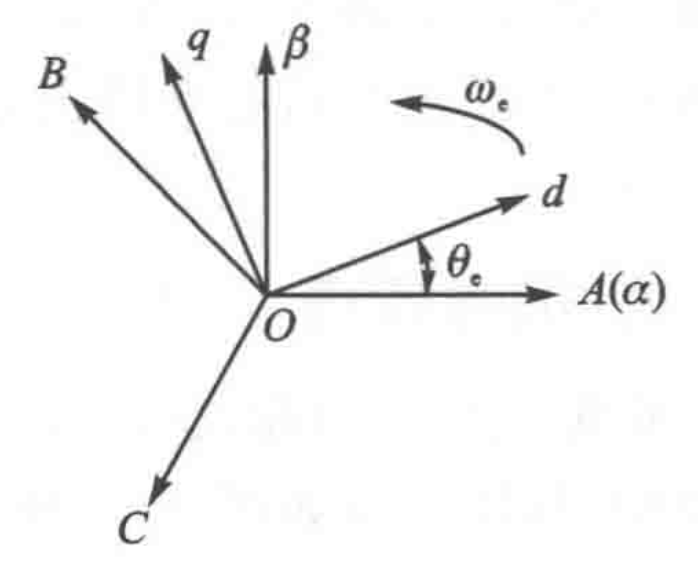
\includegraphics[width=\textwidth]{图片/三种坐标关系图.png}
        \caption{三种坐标关系图}
    \end{minipage}
    \begin{minipage}{0.5\textwidth}
        \centering
        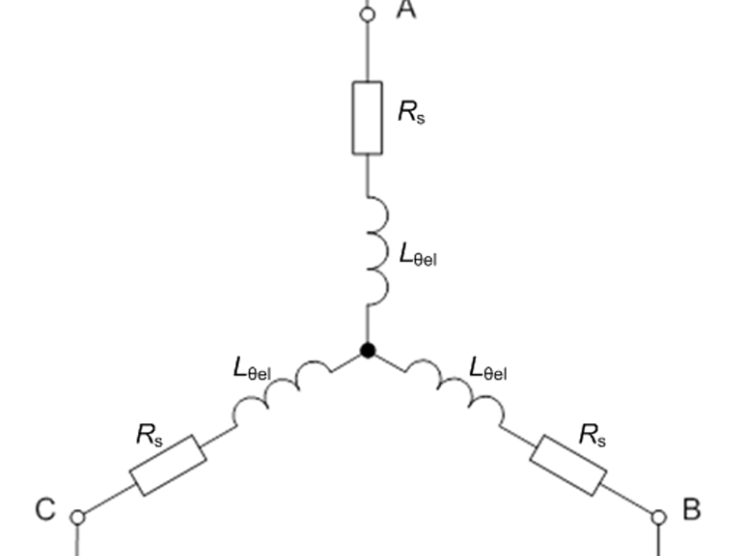
\includegraphics[width=\textwidth]{图片/三相电机电路图.PNG}
        \caption{三相电机电路图}
    \end{minipage}
\end{figure}

根据永磁体的嵌入位置，可以将永磁同步电机（PMSM）分为表贴式永磁同步电机（SPMSM）和内置式永磁同步电机（IPMSM）。
表贴式永磁同步电机是指永磁体嵌入在转子的表面，磁路对称，属于隐极电机。
而内置式永磁同步电机是指永磁体嵌入在转子的内部，磁路不对称，属于凸极电机。

接下来，讨论自然坐标系A-B-C下的永磁同步电机数学模型。对于每一相的电压、电流，
考虑存在相电阻\(R\)和相电感\(L\)。根据基尔霍夫电流定律，有\(i_{\mathrm{A}}+i_{\mathrm{B}}+i_{\mathrm{C}}=0\)。
以A相为例，在不考虑耦合时根据基尔霍夫电压定律可得
\begin{equation*}
    u_{\mathrm{A}}=R_{\mathrm{A}}i_{\mathrm{A}}+L_{\mathrm{A}}\cfrac{\dd}{\dd t}i_{\mathrm{A}}
\end{equation*}

考虑到电感之间的互感效应，会存在B、C相电感对A相电压的影响，也就有
\begin{equation*}
    u_{\mathrm{A}}=R_{\mathrm{A}}i_{\mathrm{A}}+L_{\mathrm{A}}\cfrac{\dd}{\dd t}i_{\mathrm{A}}+M_{\mathrm{BA}}\cfrac{\dd}{\dd t}i_{\mathrm{B}}+M_{\mathrm{CA}}\cfrac{\dd}{\dd t}i_{\mathrm{C}}
\end{equation*}

除此之外，转子的永磁体磁场也会对A相电感磁场造成影响。若永磁体磁链为\(\psi_{\mathrm{m}}\)，那么
永磁体磁链在三相上的分量为
\begin{equation*}
    \begin{cases}
        \psi_{\mathrm{A}}=\psi_{\mathrm{m}}\cos\theta_{\mathrm{e}}\\
        \psi_{\mathrm{B}}=-\psi_{\mathrm{m}}\cos(\cfrac{\pi}{3}+\theta_{\mathrm{e}})=
        \psi_{\mathrm{m}}\cos(\theta_{\mathrm{e}}-\cfrac{2\pi}{3})\\
        \psi_{\mathrm{C}}=-\psi_{\mathrm{m}}\cos(\cfrac{\pi}{3}-\theta_{\mathrm{e}})=
        \psi_{\mathrm{m}}\cos(\theta_{\mathrm{e}}+\cfrac{2\pi}{3})
    \end{cases}
\end{equation*}

因此完整的三相电路方程为
\begin{equation*}
    \begin{cases}
        u_{\mathrm{A}}=R_{\mathrm{A}}i_{\mathrm{A}}+L_{\mathrm{A}}\cfrac{\dd}{\dd t}i_{\mathrm{A}}+M_{\mathrm{BA}}\cfrac{\dd}{\dd t}i_{\mathrm{B}}+M_{\mathrm{CA}}
        \cfrac{\dd}{\dd t}i_{\mathrm{C}}+\cfrac{\dd}{\dd t}\psi_{\mathrm{A}}\\
        u_{\mathrm{B}}=R_{\mathrm{B}}i_{\mathrm{B}}+L_{\mathrm{B}}\cfrac{\dd}{\dd t}i_{\mathrm{B}}+M_{\mathrm{AB}}\cfrac{\dd}{\dd t}i_{\mathrm{A}}+M_{\mathrm{CB}}
        \cfrac{\dd}{\dd t}i_{\mathrm{C}}+\cfrac{\dd}{\dd t}\psi_{\mathrm{B}}\\
        u_{\mathrm{C}}=R_{\mathrm{C}}i_{\mathrm{C}}+L_{\mathrm{C}}\cfrac{\dd}{\dd t}i_{\mathrm{C}}+M_{\mathrm{AC}}\cfrac{\dd}{\dd t}i_{\mathrm{A}}+M_{\mathrm{BC}}
        \cfrac{\dd}{\dd t}i_{\mathrm{C}}+\cfrac{\dd}{\dd t}\psi_{\mathrm{C}}
    \end{cases}
\end{equation*}

用矩阵形式表示为
\begin{equation*}
    \begin{bmatrix}
        u_{\mathrm{A}}\\u_{\mathrm{B}}\\u_{\mathrm{C}}
    \end{bmatrix}
    =
    \begin{bmatrix}
        R_{\mathrm{A}}&0&0\\0&R_{\mathrm{B}}&0\\0&0&R_{\mathrm{C}}
    \end{bmatrix}
    \begin{bmatrix}
        i_{\mathrm{A}}\\i_{\mathrm{B}}\\i_{\mathrm{C}}
    \end{bmatrix}
    +
    \begin{bmatrix}
        L_{\mathrm{A}}&M_{\mathrm{BA}}&M_{\mathrm{CA}}\\
        M_{\mathrm{AB}}&L_{\mathrm{B}}&M_{\mathrm{CB}}\\
        M_{\mathrm{AC}}&M_{\mathrm{BC}}&L_{\mathrm{C}}
    \end{bmatrix}
    \begin{bmatrix}
        \cfrac{\dd}{\dd t}i_{\mathrm{A}}\\
        \cfrac{\dd}{\dd t}i_{\mathrm{B}}\\
        \cfrac{\dd}{\dd t}i_{\mathrm{C}}
    \end{bmatrix}
    -
    \psi_{\mathrm{m}}\omega_{\mathrm{e}}
    \begin{bmatrix}
        \sin\theta_{\mathrm{e}}\\
        \sin(\theta_{\mathrm{e}}-\cfrac{2\pi}{3})\\
        \sin(\theta_{\mathrm{e}}+\cfrac{2\pi}{3})
    \end{bmatrix}
\end{equation*}

需要注意的是，若永磁同步电机为凸极电机（IPMSM），那么电感（包括自感和互感）
不是常数，其值会随着电角度而发生变化。自感值和互感值可以用下式表示。存在电角度的二次谐波，其主要原因是
对于定子而言，不对称的椭圆磁路每转过180°电角度，永磁体对其的影响就发生一个周期的变化。
\begin{minipage}{0.5\textwidth}
    \begin{equation*}
        \begin{cases}
            L_{\mathrm{A}}=L_{\mathrm{A}0}-L_{\mathrm{A}2}\cos2\theta_{\mathrm{e}}\\
            L_{\mathrm{B}}=L_{\mathrm{B}0}-L_{\mathrm{B}2}\cos(2\theta_{\mathrm{e}}-\cfrac{4\pi}{3})\\
            L_{\mathrm{C}}=L_{\mathrm{C}0}-L_{\mathrm{C}2}\cos(2\theta_{\mathrm{e}}+\cfrac{4\pi}{3})
        \end{cases}
    \end{equation*}
\end{minipage}
\begin{minipage}{0.5\textwidth}
    \begin{equation*}
        \begin{cases}
            M_{\mathrm{AB}}=M_{\mathrm{BA}}=M_{\mathrm{AB}0}-M_{\mathrm{AB}2}\cos(2\theta_{\mathrm{e}}+\cfrac{4\pi}{3})\\
            M_{\mathrm{BC}}=M_{\mathrm{CB}}=M_{\mathrm{BC}0}-M_{\mathrm{BC}2}\cos2\theta_{\mathrm{e}}\\
            M_{\mathrm{AC}}=M_{\mathrm{CA}}=M_{\mathrm{AC}0}-M_{\mathrm{AC}2}\cos(2\theta_{\mathrm{e}}-\cfrac{4\pi}{3})
        \end{cases}
    \end{equation*}
\end{minipage}

理想情况下电机为三相对称电路，即有
\(\begin{cases}
    R_{\mathrm{A}}=R_{\mathrm{B}}=R_{\mathrm{C}}=R_{\mathrm{s}}\\
    L_{\mathrm{A}0}=L_{\mathrm{B}0}=L_{\mathrm{C}0}=L_{\mathrm{s}0}\\
    L_{\mathrm{A}2}=L_{\mathrm{B}2}=L_{\mathrm{C}2}=L_{\mathrm{s}2}\\
    M_{\mathrm{AB}0}=M_{\mathrm{BC}0}=M_{\mathrm{AC}0}=M_{\mathrm{s}0}\\
    M_{\mathrm{AB}2}=M_{\mathrm{BC}2}=M_{\mathrm{AC}2}=M_{\mathrm{s}2}
\end{cases}\)，

那么电路方程可以简化表示为
\begin{equation*}
    \begin{bmatrix}
        u_{\mathrm{A}}\\u_{\mathrm{B}}\\u_{\mathrm{C}}
    \end{bmatrix}
    =
    R_{\mathrm{s}}
    \begin{bmatrix}
        i_{\mathrm{A}}\\i_{\mathrm{B}}\\i_{\mathrm{C}}
    \end{bmatrix}
    +
    \cfrac{\dd}{\dd t}
    \Big(\bm{L}(\theta_{\mathrm{e}})
    \begin{bmatrix}
        i_{\mathrm{A}}\\i_{\mathrm{B}}\\i_{\mathrm{C}}
    \end{bmatrix}
    \Big)-
    \psi_{\mathrm{m}}\omega_{\mathrm{e}}
    \begin{bmatrix}
        \sin\theta_{\mathrm{e}}\\
        \sin(\theta_{\mathrm{e}}-\cfrac{2\pi}{3})\\
        \sin(\theta_{\mathrm{e}}+\cfrac{2\pi}{3})
    \end{bmatrix}
\end{equation*}

对微分项展开可得
\(\cfrac{\dd}{\dd t}\Big(\bm{L}(\theta_{\mathrm{e}})
\begin{bmatrix}
    {{i_{\mathrm{A}}}}\\{{i_{\mathrm{B}}}}\\{{i_{\mathrm{C}}}}
\end{bmatrix}\Big)
=
\cfrac{\dd}{\dd t}\bm{L}(\theta_{\mathrm{e}})
\begin{bmatrix}
    i_{\mathrm{A}}\\i_{\mathrm{B}}\\i_{\mathrm{C}}
\end{bmatrix}
+
\bm{L}(\theta_{\mathrm{e}})
\begin{bmatrix}
    \dot{i_{\mathrm{A}}}\\\dot{i_{\mathrm{B}}}\\\dot{i_{\mathrm{C}}}
\end{bmatrix}\)
\footnote{\(\dot{x}\)表示对信号\(x\)进行时间微分，即
\(\dot{x}=\cfrac{\dd x}{\dd t}\)}

电感矩阵微分为
\begin{equation}
    \cfrac{\dd}{\dd t}\bm{L}(\theta_{\mathrm{e}})
    =2\omega_{\mathrm{e}}
    \begin{bmatrix}
        L_{\mathrm{s}2}\sin2\theta_{\mathrm{e}}
        &M_{\mathrm{s}2}\sin(2\theta_{\mathrm{e}}+\cfrac{4\pi}{3})
        &M_{\mathrm{s}2}\sin(2\theta_{\mathrm{e}}-\cfrac{4\pi}{3})
        \\
        M_{\mathrm{s}2}\sin(2\theta_{\mathrm{e}}+\cfrac{4\pi}{3})
        &L_{\mathrm{s}2}\sin(2\theta_{\mathrm{e}}-\cfrac{4\pi}{3})
        &M_{\mathrm{s}2}\sin2\theta_{\mathrm{e}}
        \\
        M_{\mathrm{s}2}\sin(2\theta_{\mathrm{e}}-\cfrac{4\pi}{3})
        &M_{\mathrm{s}2}\sin2\theta_{\mathrm{e}}
        &L_{\mathrm{s}2}\sin(2\theta_{\mathrm{e}}+\cfrac{4\pi}{3})
    \end{bmatrix}
    \label{eq:电感矩阵微分}
\end{equation}

因此完整的电路表达式如下式表示：
\begin{align*}
    \begin{bmatrix}
        u_{\mathrm{A}} \\ u_{\mathrm{B}} \\ u_{\mathrm{C}}
    \end{bmatrix} &=
    \begin{bmatrix}
        2\omega_{\mathrm{e}}L_{\mathrm{s}2}\sin2\theta_{\mathrm{e}}+R_{\mathrm{s}}
        & 2\omega_{\mathrm{e}}M_{\mathrm{s}2}\sin(2\theta_{\mathrm{e}}+\cfrac{4\pi}{3})
        & 2\omega_{\mathrm{e}}M_{\mathrm{s}2}\sin(2\theta_{\mathrm{e}}-\cfrac{4\pi}{3})
        \\
        2\omega_{\mathrm{e}}M_{\mathrm{s}2}\sin(2\theta_{\mathrm{e}}+\cfrac{4\pi}{3})
        & 2\omega_{\mathrm{e}}L_{\mathrm{s}2}\sin2(\theta_{\mathrm{e}}-\cfrac{4\pi}{3})+R_{\mathrm{s}}
        & 2\omega_{\mathrm{e}}M_{\mathrm{s}2}\sin2\theta_{\mathrm{e}}
        \\
        2\omega_{\mathrm{e}}M_{\mathrm{s}2}\sin(2\theta_{\mathrm{e}}-\cfrac{4\pi}{3})
        & 2\omega_{\mathrm{e}}M_{\mathrm{s}2}\sin2\theta_{\mathrm{e}}
        & 2\omega_{\mathrm{e}}L_{\mathrm{s}2}\sin(2\theta_{\mathrm{e}}+\cfrac{4\pi}{3})+R_{\mathrm{s}}
    \end{bmatrix}
    \begin{bmatrix}
        i_{\mathrm{A}} \\ i_{\mathrm{B}} \\ i_{\mathrm{C}}
    \end{bmatrix} \\
    & +
    \begin{bmatrix}
        L_{\mathrm{s}0}-L_{\mathrm{s}2}\cos2\theta_{\mathrm{e}}
        & M_{\mathrm{s}0}-M_{\mathrm{s}2}\cos(2\theta_{\mathrm{e}}+\cfrac{4\pi}{3})
        & M_{\mathrm{s}0}-M_{\mathrm{s}2}\cos(2\theta_{\mathrm{e}}-\cfrac{4\pi}{3})
        \\
        M_{\mathrm{s}0}-M_{\mathrm{s}2}\cos(2\theta_{\mathrm{e}}+\cfrac{4\pi}{3})
        & L_{\mathrm{s}0}-L_{\mathrm{s}2}\cos(2\theta_{\mathrm{e}}-\cfrac{4\pi}{3})
        & M_{\mathrm{s}0}-M_{\mathrm{s}2}\cos2\theta_{\mathrm{e}}
        \\
        M_{\mathrm{s}0}-M_{\mathrm{s}2}\cos(2\theta_{\mathrm{e}}-\cfrac{4\pi}{3})
        & M_{\mathrm{s}0}-M_{\mathrm{s}2}\cos2\theta_{\mathrm{e}}
        & L_{\mathrm{s}0}-L_{\mathrm{s}2}\cos(2\theta_{\mathrm{e}}+\cfrac{4\pi}{3})
    \end{bmatrix}
    \begin{bmatrix}
        \dot{i_{\mathrm{A}}} \\ \dot{i_{\mathrm{B}}} \\ \dot{i_{\mathrm{C}}}
    \end{bmatrix} \\
    & -
    \psi_{\mathrm{m}}\omega_{\mathrm{e}}
    \begin{bmatrix}
        \sin\theta_{\mathrm{e}} \\
        \sin(\theta_{\mathrm{e}}-\cfrac{2\pi}{3}) \\
        \sin(\theta_{\mathrm{e}}+\cfrac{2\pi}{3})
    \end{bmatrix}
\end{align*}

为了简化表示，定义向量
\(
\bm{U}_{\mathrm{ABC}}=
\begin{bmatrix}
    u_{\mathrm{A}}\\u_{\mathrm{B}}\\u_{\mathrm{C}}
\end{bmatrix},
\bm{I}_{\mathrm{ABC}}=
\begin{bmatrix}
    i_{\mathrm{A}}\\i_{\mathrm{B}}\\i_{\mathrm{C}}
\end{bmatrix},
\bm{L}_{\mathrm{ABC}}=
\bm{L}(\theta),
\bm{\varPsi}_{\mathrm{ABC}}=
\begin{bmatrix}
    \psi_{\mathrm{A}}\\\psi_{\mathrm{B}}\\\psi_{\mathrm{C}}
\end{bmatrix}
=\psi_{\mathrm{m}}
\begin{bmatrix}\cos\theta_{\mathrm{e}}\\
    \cos(\theta_{\mathrm{e}}-\cfrac{2\pi}{3})\\
    \cos(\theta_{\mathrm{e}}+\cfrac{2\pi}{3})
\end{bmatrix}
\)
那么电路方程可以表示为
\begin{equation}
    \bm{U}_{\mathrm{ABC}}=
    R_{\mathrm{s}}\bm{I}_{\mathrm{ABC}}+
    {\dot{\bm{L}}_{\mathrm{ABC}}\bm{I}_{\mathrm{ABC}}+
    \bm{L}_{\mathrm{ABC}}\dot{\bm{I}}_{\mathrm{ABC}}}
    +{\dot{\bm{\varPsi}}_{\mathrm{ABC}}}
    \label{eq:自然坐标系电路方程}
\end{equation}

接下来讨论自然坐标系下永磁同步电机的电磁转矩表达式，这是连接电路和机械运动的关
键方程。首先，机械角度\(\theta_{\mathrm{m}}\)、机械角速度\(\omega_{\mathrm{m}}\)、
电角度\(\theta_{\mathrm{e}}\)、电角速度与电机的磁极对数\(p\)满足    
\(p\omega_{\mathrm{m}}=\omega_{\mathrm{e}},p\theta_{\mathrm{m}}=\theta_{\mathrm{e}}\)。

从能量守恒角度分析，电机中的功率总表达式为
\(P_{\mathrm{in}}=P_{\mathrm{Cu}}+\cfrac{\dd W_{\mathrm{m}}}{\dd t}+P_{\mathrm{e}}\)
。其中\(P_{\mathrm{in}}\)表示输入功率，\(P_{\mathrm{Cu}}\)表示定子铜损，
\(\cfrac{\dd W_{\mathrm{m}}}{\dd t}\)表示维持磁场的无功功率
，\(P_{\mathrm{e}}\)表示电磁功率。也就是说电磁功率可以表示为
\(P_{\mathrm{e}}=P_{\mathrm{in}}-P_{\mathrm{Cu}}-\cfrac{\dd W_{\mathrm{m}}}{\dd t}\)

定子铜损即相电阻上消耗的电功率，计算式为\(P_{\mathrm{Cu}}=R_{\mathrm{s}}(i_{\mathrm{A}}^2+i_{\mathrm{B}}^2+i_{\mathrm{C}}^2)\)
用矩阵表示为
\begin{equation*}
    P_{\mathrm{Cu}}=R_{\mathrm{s}}\bm{I}^T_{\mathrm{ABC}}\bm{I}_{\mathrm{ABC}}
\end{equation*}

电磁功率即输出的功率，和电磁转矩与机械角速度满足
\begin{equation*}
    P_{\mathrm{e}}=T_{\mathrm{e}}\omega_{\mathrm{m}}
\end{equation*}

无功功率主要用于维持磁场。根据磁场能表达式\(W_{\mathrm{m}}=\cfrac 12 LI^2\)，因此无功功率有：
\begin{equation*}
    \cfrac{\dd W_{\mathrm{m}}}{\dd t}=\cfrac 12
\cfrac{\dd}{\dd t}\bm{I}^T_{\mathrm{ABC}}\bm{L}_{\mathrm{ABC}}\bm{I}_{\mathrm{ABC}}
\end{equation*}

根据微分链式法则可以展开为三项之和：
\begin{equation*}
    \cfrac{\dd W_{\mathrm{m}}}{\dd t}=
\cfrac 12
(\dot{\bm{I}}^T_{\mathrm{ABC}}\bm{L}_{\mathrm{ABC}}\bm{I}_{\mathrm{ABC}}+
\bm{I}^T_{\mathrm{ABC}}\dot{\bm{L}}_{\mathrm{ABC}}\bm{I}_{\mathrm{ABC}}+
\bm{I}^T_{\mathrm{ABC}}\bm{L}_{\mathrm{ABC}}\dot{\bm{I}}_{\mathrm{ABC}})
\end{equation*}

由于\(\bm{L}_{\mathrm{ABC}}\)为对称矩阵，
因此\(\dot{\bm{I}}^T_{\mathrm{ABC}}\bm{L}_{\mathrm{ABC}}\bm{I}_{\mathrm{ABC}}
=\bm{I}^T_{\mathrm{ABC}}\bm{L}_{\mathrm{ABC}}\dot{\bm{I}}_{\mathrm{ABC}}\)
也就可得
\begin{equation*}
    \cfrac{\dd W_{\mathrm{m}}}{\dd t}=
\dot{\bm{I}}^T_{\mathrm{ABC}}\bm{L}_{\mathrm{ABC}}\bm{I}_{\mathrm{ABC}}+
\cfrac 12\bm{I}^T_{\mathrm{ABC}}\dot{\bm{L}}_{\mathrm{ABC}}\bm{I}_{\mathrm{ABC}}
\end{equation*}

电机的输入功率表达式为\(P_{\mathrm{in}}=\bm{U}_{\mathrm{ABC}}^T\bm{I}_{\mathrm{ABC}}\)
展开得到：
\begin{equation*}
    P=R_{\mathrm{s}}\bm{I}^T_{\mathrm{ABC}}\bm{I}_{\mathrm{ABC}}+\bm{I}^T_{\mathrm{ABC}}
\dot{\bm{L}}^T_{\mathrm{ABC}}\bm{I}_{\mathrm{ABC}}+\dot{\bm{I}}^T_{\mathrm{ABC}}
\bm{L}^T_{\mathrm{ABC}}\bm{I}_{\mathrm{ABC}}+\dot{\bm{\varPsi}}^T_{\mathrm{ABC}}\bm{I}_{\mathrm{ABC}}
\end{equation*}

由于电感矩阵为对称矩阵，因此可以表示为
\begin{equation*}
    P=R_{\mathrm{s}}\bm{I}^T_{\mathrm{ABC}}\bm{I}_{\mathrm{ABC}}+
    \bm{I}^T_{\mathrm{ABC}}\dot{\bm{L}}_{\mathrm{ABC}}\bm{I}_{\mathrm{ABC}}+
    {\bm{I}}^T_{\mathrm{ABC}}\bm{L}_{\mathrm{ABC}}\bm{I}_{\mathrm{ABC}}+
    \dot{\bm{\varPsi}}^T_{\mathrm{ABC}}\bm{I}_{\mathrm{ABC}}  
\end{equation*}

根据输入功率表达式可知：
\begin{equation*}
    P_{\mathrm{e}}=P-R_{\mathrm{s}}\bm{I}^T_{\mathrm{ABC}}\bm{I}_{\mathrm{ABC}}-
(\dot{\bm{I}}^T_{\mathrm{ABC}}\bm{L}_{\mathrm{ABC}}\bm{I}_{\mathrm{ABC}}
+\cfrac 12\bm{I}^T_{\mathrm{ABC}}\dot{\bm{L}}_{\mathrm{ABC}}\bm{I}_{\mathrm{ABC}})
\end{equation*}

可得电磁功率表达式为：
\begin{equation*}
    P_{\mathrm{e}}=\cfrac 12\bm{I}^T_{\mathrm{ABC}}\dot{\bm{L}}_{\mathrm{ABC}}
\bm{I}_{\mathrm{ABC}}+\dot{\bm{\varPsi}}^T_{\mathrm{ABC}}\bm{I}_{\mathrm{ABC}}
\end{equation*}

两边除以机械角速度即可得到电磁转矩表达式
\begin{equation}
    T_{\mathrm{e}}=\cfrac{1}{\omega_{\mathrm{m}}}
    (\cfrac 12\bm{I}^T_{\mathrm{ABC}}\dot{\bm{L}}_{\mathrm{ABC}}\bm{I}_{\mathrm{ABC}}
    +\dot{\bm{\varPsi}}^T_{\mathrm{ABC}}\bm{I}_{\mathrm{ABC}})
    \label{eq:自然坐标系电磁转矩表达式}
\end{equation}

\subsection{克拉克变换与帕克变换}
根据\ref{sec:基本数学方程}中的推导可知，在A-B-C三相自然坐标系下描述永磁同步电机的行为是非常复杂的。
因此更常采用坐标变换的方法，将三相自然坐标系转换为更方便描述的同步旋转坐标系。
这一过程需要通过克拉克变换和帕克变换两个步骤。

克拉克变换旨在将A-B-C三相自然坐标系转换为正交基底的两相静止坐标系\(\alpha-\beta\)，
。两个坐标系的关系如下图所示
\begin{figure}[H]
    \centering
    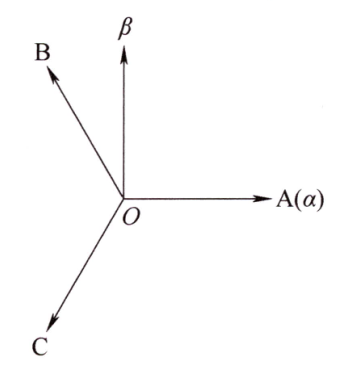
\includegraphics[width=0.4\textwidth]
    {图片/克拉克变换.png}
    \caption{克拉克变换}
\end{figure}

根据线性变换的知识，三相自然坐标系下的三个相差120°的单位向量，在两相静止坐标系下
可以表示为
\(
\begin{bmatrix}
    1&-\cfrac12&-\cfrac12\\
    0&\cfrac{\sqrt{3}}{2}&-\cfrac{\sqrt{3}}{2}
\end{bmatrix}
\)
，为了便于后续的计算，会进行等幅值变换，即希望变换前后满足\(i_{\mathrm{A}}=i_{\mathrm{\alpha}}\)，也就是
确定常数\(k\)使得
\(
k
\begin{bmatrix}
    1&-\cfrac12&-\cfrac12\\
    0&\cfrac{\sqrt{3}}{2}&-\cfrac{\sqrt{3}}{2}
\end{bmatrix}
\begin{bmatrix}
    1\\-\cfrac 12\\-\cfrac 12
\end{bmatrix}
=\begin{bmatrix}1\\0\end{bmatrix}
\)
，可以解得\(k=\cfrac 23\)。

此外，三相自然坐标系是三维的，而两相静止坐标系是二维的。为了方便矩阵求逆，也为了
描述三相电机的电流制约关系，会加入零序分量\(i_{\mathrm{0}}=\cfrac{1}{3}(i_{\mathrm{A}}+i_{\mathrm{B}}+i_{\mathrm{C}})=0\)。

最终得到克拉克变换公式
\begin{equation}
    \begin{bmatrix}
        i_{\mathrm{\alpha}}\\i_{\mathrm{\beta}}\\i_{\mathrm{0}}
    \end{bmatrix}
    =\cfrac 23
    \begin{bmatrix}
        1&-\cfrac12&-\cfrac12
        \\0&\cfrac{\sqrt{3}}{2}&-\cfrac{\sqrt{3}}{2}\\
        \cfrac{1}{2}&\cfrac{1}{2}&\cfrac{1}{2}
    \end{bmatrix}
    \begin{bmatrix}
        i_{\mathrm{A}}\\i_{\mathrm{B}}\\i_{\mathrm{C}}
    \end{bmatrix}
    \label{eq:克拉克变换}
\end{equation}

对于矩阵求逆可得克拉克逆变换公式
\begin{equation}
    \begin{bmatrix}
        i_{\mathrm{A}}\\i_{\mathrm{B}}\\i_{\mathrm{C}}
    \end{bmatrix}
    =\begin{bmatrix}
        1&0&1
        \\-\cfrac 12&\cfrac{\sqrt{3}}{2}&1
        \\-\cfrac 12&-\cfrac{\sqrt{3}}{2}&1
    \end{bmatrix}
    \begin{bmatrix}
        i_{\mathrm{\alpha}}\\i_{\mathrm{\beta}}\\i_{\mathrm{0}}
    \end{bmatrix}
    \label{eq:克拉克逆变换}
\end{equation}

接下来需要进行帕克变换，实现从两相静止坐标系到同步旋转坐标系的变换。定义沿着永磁
体旋转方向，与永磁体磁链同方向的轴为直轴d/D，超前直轴90°为交轴q/Q。d轴与
\(\mathrm{A(\alpha)}\)的夹角就是电角度\(\theta_{\mathrm{e}}\)
\begin{figure}[H]
    \centering
    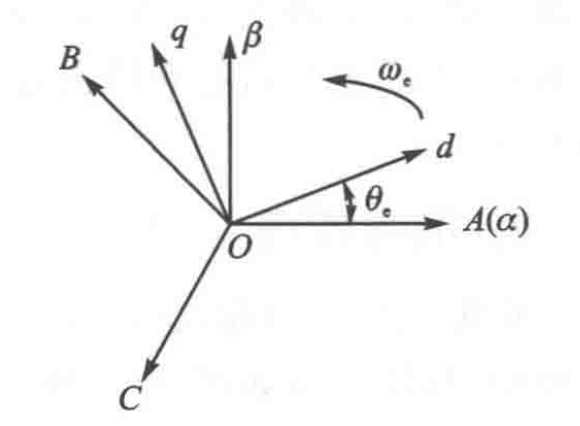
\includegraphics[width=0.4\textwidth]
    {图片/帕克变换.png}
    \caption{帕克变换}
\end{figure}

两相静止坐标系在的单位矢量在同步旋转坐标系下表示为
\(
\begin{bmatrix}
    \cos\theta_{\mathrm{e}}&\sin\theta_{\mathrm{e}}\\-\sin\theta_{\mathrm{e}}&\cos\theta_{\mathrm{e}}
\end{bmatrix}\)
可得帕克变换公式为
\begin{equation}
    \begin{bmatrix}
        i_{\mathrm{d}}\\i_{\mathrm{q}}\\i_{\mathrm{0}}
    \end{bmatrix}
    =
    \begin{bmatrix}
        \cos\theta_{\mathrm{e}}&\sin\theta_{\mathrm{e}}&0
        \\-\sin\theta_{\mathrm{e}}&\cos\theta_{\mathrm{e}}&0
        \\0&0&1
    \end{bmatrix}
    \begin{bmatrix}
        i_{\mathrm{\alpha}}
            \\i_{\mathrm{\beta}}
            \\i_{\mathrm{0}}
    \end{bmatrix}
    \label{eq:帕克变换}
\end{equation}

而帕克逆变换公式为
\begin{equation}
    \begin{bmatrix}
        i_{\mathrm{\alpha}}\\i_{\mathrm{\beta}}\\i_{\mathrm{0}}
    \end{bmatrix}
    =
    \begin{bmatrix}
        \cos\theta_{\mathrm{e}}&-\sin\theta_{\mathrm{e}}&0\\
        \sin\theta_{\mathrm{e}}&\cos\theta_{\mathrm{e}}&0\\
        0&0&1
    \end{bmatrix}
    \begin{bmatrix}
        i_{\mathrm{d}}\\i_{\mathrm{q}}\\i_{\mathrm{0}}
    \end{bmatrix}
    \label{eq:帕克逆变换}
\end{equation}

有时也可以把克拉克变换和帕克变换合并起来，直接从三相自然坐标系
到同步旋转坐标系的变换，该变换表达式为
\begin{equation}
    \begin{bmatrix}
        i_{\mathrm{d}}\\i_{\mathrm{q}}\\i_{\mathrm{0}}
    \end{bmatrix}
    =
    \cfrac 23
    \begin{bmatrix}
        \cos\theta_{\mathrm{e}}&\cos(\theta_{\mathrm{e}}-\cfrac{2\pi}{3})
        &\cos(\theta_{\mathrm{e}}+\cfrac{2\pi}{3})
        \\-\sin\theta_{\mathrm{e}}&-\sin(\theta_{\mathrm{e}}-\cfrac{2\pi}{3})
        &-\sin(\theta_{\mathrm{e}}+\cfrac{2\pi}{3})\\
        \cfrac 12&\cfrac 12&\cfrac 12
    \end{bmatrix}
    \begin{bmatrix}i_{\mathrm{A}}\\i_{\mathrm{B}}\\i_{\mathrm{C}}\end{bmatrix}
    =\bm{T}\begin{bmatrix}i_{\mathrm{A}}\\i_{\mathrm{B}}\\i_{\mathrm{C}}\end{bmatrix}
    \label{eq:克拉克-帕克变换}
\end{equation}

其中克拉克-帕克变换矩阵
\(\bm{T}=\cfrac 23
\begin{bmatrix}
    \cos\theta_{\mathrm{e}}&\cos(\theta_{\mathrm{e}}-\cfrac{2\pi}{3})
    &\cos(\theta_{\mathrm{e}}+\cfrac{2\pi}{3})\\
    -\sin\theta_{\mathrm{e}}&-\sin(\theta_{\mathrm{e}}-\cfrac{2\pi}{3})
    &-\sin(\theta_{\mathrm{e}}+\cfrac{2\pi}{3})\\
    \cfrac 12&\cfrac 12&\cfrac 12
\end{bmatrix}\)

\subsection{同步旋转坐标系下的数学模型}

接下来，利用克拉克变换和帕克变换，主要是公式\eqref{eq:克拉克-帕克变换}，分析如何将
自然坐标系下表示的电路方程\eqref{eq:自然坐标系电路方程}和电磁转矩表达式
\eqref{eq:自然坐标系电磁转矩表达式}转换为同步旋转坐标系下表示。

首先需要计算变换矩阵\(\bm{T}\)的逆矩阵\(\bm{T}^{-1}\)和微分逆矩阵\(\cfrac{\dd}{\dd t}\bm{T}^{-1}\)，
这会在后续计算中使用到
\begin{equation}
    \bm{T}^{-1}
    =
    \begin{bmatrix}\cos\theta_{\mathrm{e}}&-\sin\theta_{\mathrm{e}}&1\\
        \cos(\theta_{\mathrm{e}}-\cfrac{2\pi}{3})&-\sin(\theta_{\mathrm{e}}-\cfrac{2\pi}{3})&1\\
        \cos(\theta_{\mathrm{e}}+\cfrac{2\pi}{3})&-\sin(\theta_{\mathrm{e}}+\cfrac{2\pi}{3})&1
    \end{bmatrix}
    \label{eq:克拉克-帕克变换矩阵逆矩阵}
\end{equation}
\begin{equation}
    \cfrac{\dd}{\dd t}\bm{T}^{-1}
    =\omega_{\mathrm{e}}\begin{bmatrix}-\sin\theta_{\mathrm{e}}&-\cos\theta_{\mathrm{e}}&0\\
        -\sin(\theta_{\mathrm{e}}-\cfrac{2\pi}{3})&-\cos(\theta_{\mathrm{e}}-\cfrac{2\pi}{3})&0\\
        -\sin(\theta_{\mathrm{e}}+\cfrac{2\pi}{3})&-\cos(\theta_{\mathrm{e}}+\cfrac{2\pi}{3})&0
    \end{bmatrix}
    \label{eq:克拉克-帕克变换矩阵微分逆矩阵}
\end{equation}

针对电路方程，同时左乘变换矩阵\(\bm{T}\)，可得
\begin{equation*}
    \bm{T}\bm{U}_{\mathrm{ABC}}
    =\bm{T}R_{\mathrm{s}}\bm{I}_{\mathrm{ABC}}+
    \bm{T}{\dot{\bm{L}}_{\mathrm{ABC}}\bm{I}_{\mathrm{ABC}}+
    \bm{T}\bm{L}_{\mathrm{ABC}}\dot{\bm{I}}_{\mathrm{ABC}}}+
    \bm{T}{\dot{\bm{\varPsi}}_{\mathrm{ABC}}}
\end{equation*}

其中
\(
\bm{T}\bm{U}_{\mathrm{ABC}}
=\begin{bmatrix}u_{\mathrm{d}}\\u_{\mathrm{q}}\\u_{\mathrm{0}}\end{bmatrix}
,\bm{T}R_{\mathrm{s}}\bm{I}_{\mathrm{ABC}}=R_{\mathrm{s}}\begin{bmatrix}i_{\mathrm{d}}\\i_{\mathrm{q}}\\i_{\mathrm{0}}\end{bmatrix}
\)
形式较为简单。

接下考虑\(\bm{T}\dot{\bm{L}}_{\mathrm{ABC}}\bm{I}_{\mathrm{ABC}}\)。根据矩阵乘法定律，
直接交换矩阵乘法是有风险的，因此考虑直接使用
\(\bm{I}_{\mathrm{ABC}}=\bm{T}^{-1}\begin{bmatrix}i_{\mathrm{d}}\\i_{\mathrm{q}}\\i_{\mathrm{0}}\end{bmatrix}\)
进行代换得到
\(\bm{T}\dot{\bm{L}}_{\mathrm{ABC}}\bm{T}^{-1}\begin{bmatrix}i_{\mathrm{d}}\\i_{\mathrm{q}}\\i_{\mathrm{0}}\end{bmatrix}\)
根据公式\eqref{eq:电感矩阵微分}\eqref{eq:克拉克-帕克变换}和
\eqref{eq:克拉克-帕克变换矩阵逆矩阵}，通过计算可得
\begin{equation*}
    \bm{T}\dot{\bm{L}}_{\mathrm{ABC}}\bm{I}_{\mathrm{ABC}}=
    \begin{bmatrix}
        0&-\omega_{\mathrm{e}}(L_{\mathrm{s}2}+2M_{\mathrm{s}2})&2\omega_{\mathrm{e}}\sin(3\theta_{\mathrm{e}})(L_{\mathrm{s}2}-M_{\mathrm{s}2})
        \\-\omega_{\mathrm{e}}(L_{\mathrm{s}2}+2M_{\mathrm{s}2})&0&2\omega_{\mathrm{e}}\cos(3\theta_{\mathrm{e}})(L_{\mathrm{s}2}-M_{\mathrm{s}2})
        \\\omega_{\mathrm{e}}\sin(3\theta_{\mathrm{e}})(L_{\mathrm{s}2}-M_{\mathrm{s}2})
        &\omega_{\mathrm{e}}\cos(3\theta_{\mathrm{e}})(L_{\mathrm{s}2}-M_{\mathrm{s}2})&0
    \end{bmatrix}
    \begin{bmatrix}i_{\mathrm{d}}\\i_{\mathrm{q}}\\i_{\mathrm{0}}\end{bmatrix}
\end{equation*}

接下来计算\(\bm{T}\bm{L}_{\mathrm{ABC}}\dot{\bm{I}}_{\mathrm{ABC}}\)。
代入\(\bm{T}\bm{I}_{\mathrm{ABC}}=\begin{bmatrix}i_{\mathrm{d}}\\i_{\mathrm{q}}\\i_{\mathrm{0}}\end{bmatrix}\)可得：
\begin{equation*}
\bm{T}\bm{L}_{\mathrm{ABC}}\dot{\bm{I}}_{\mathrm{ABC}}
=\bm{T}\bm{L}_{\mathrm{ABC}}(\cfrac{\dd}{\dd t}\bm{T}^{-1}
\begin{bmatrix}i_{\mathrm{d}}\\i_{\mathrm{q}}\\i_{\mathrm{0}}\end{bmatrix}
+\bm{T}^{-1}\begin{bmatrix}\dot{i_{\mathrm{d}}}\\\dot{i_{\mathrm{q}}}\\\dot{i_{\mathrm{0}}}\end{bmatrix})
=\bm{T}\bm{L}_{\mathrm{ABC}}\cfrac{\dd}{\dd t}\bm{T}^{-1}
\begin{bmatrix}i_{\mathrm{d}}\\i_{\mathrm{q}}\\i_{\mathrm{0}}\end{bmatrix}
+\bm{T}\bm{L}_{\mathrm{ABC}}\bm{T}^{-1}
\begin{bmatrix}\dot{i_{\mathrm{d}}}\\\dot{i_{\mathrm{q}}}\\\dot{i_{\mathrm{0}}}\end{bmatrix}
\end{equation*}

根据公式\eqref{eq:克拉克-帕克变换}\eqref{eq:克拉克-帕克变换矩阵逆矩阵}
\eqref{eq:克拉克-帕克变换矩阵微分逆矩阵}
分别计算\(\bm{T}\bm{L}_{\mathrm{ABC}}\bm{T}^{-1}
\begin{bmatrix}\dot{i_{\mathrm{d}}}\\\dot{i_{\mathrm{q}}}\\\dot{i_{\mathrm{0}}}\end{bmatrix}\)和
\(\bm{T}\bm{L}_{\mathrm{ABC}}\cfrac{\dd}{\dd t}\bm{T}^{-1}
\begin{bmatrix}i_{\mathrm{d}}\\i_{\mathrm{q}}\\i_{\mathrm{0}}\end{bmatrix}\)即可。最终计算得到
\begin{align*}
    \bm{T}\bm{L}_{\mathrm{ABC}}\dot{\bm{I}}_{\mathrm{ABC}} & =
    \begin{bmatrix}
        0&\omega_{\mathrm{e}}(\cfrac{L_{\mathrm{s}2}}2-L_{\mathrm{s}0}+M_{\mathrm{s}0}+M_{\mathrm{s}2})&0\\
        \omega_{\mathrm{e}}(\cfrac{L_{\mathrm{s}2}}2+L_{\mathrm{s}0}-M_{\mathrm{s}0}+M_{\mathrm{s}2})&0&0\\
        \cfrac {\omega_{\mathrm{e}}\sin(3\theta_{\mathrm{e}})(L_{\mathrm{s}2}-M_{\mathrm{s}2})}{2}
        &\cfrac {\omega_{\mathrm{e}}\cos(3\theta_{\mathrm{e}})(L_{\mathrm{s}2}-M_{\mathrm{s}2})}{2}&0
    \end{bmatrix}
    \begin{bmatrix}i_{\mathrm{d}}\\i_{\mathrm{q}}\\i_{\mathrm{0}}\end{bmatrix}\\
    &+
    \begin{bmatrix}
        L_{\mathrm{s}0}-\cfrac{L_{\mathrm{s}2}}{2}-M_{\mathrm{s}0}-M_{\mathrm{s}2}&0
        &-\cos(3\theta_{\mathrm{e}})(L_{\mathrm{s}2}-M_{\mathrm{s}2})
        \\0&L_{\mathrm{s}0}+\cfrac{L_{\mathrm{s}2}}{2}-M_{\mathrm{s}0}+M_{\mathrm{s}2}
        &\sin(3\theta_{\mathrm{e}})(L_{\mathrm{s}2}-M_{\mathrm{s}2})\\
        -\cfrac {\cos(3\theta_{\mathrm{e}})(L_{\mathrm{s}2}-M_{\mathrm{s}2})}{2}
        &\cfrac {\sin(3\theta_{\mathrm{e}})(L_{\mathrm{s}2}-M_{\mathrm{s}2})}{2}&L_{\mathrm{s}0}+2M_{\mathrm{s}0}
    \end{bmatrix}
    \begin{bmatrix}\dot{i_{\mathrm{d}}}\\\dot{i_{\mathrm{q}}}\\\dot{i_{\mathrm{0}}}\end{bmatrix}
\end{align*}

最后计算\(\bm{T}\dot{\bm{\varPsi}}_{\mathrm{ABC}}\)。根据
\(\bm{\varPsi}_{\mathrm{ABC}}=
\psi_{\mathrm{m}}
\begin{bmatrix}\cos\theta_{\mathrm{e}}\\
    \cos(\theta_{\mathrm{e}}-\cfrac{2\pi}{3})\\
    \cos(\theta_{\mathrm{e}}+\cfrac{2\pi}{3})
\end{bmatrix}\)
可得
\(\bm{T}\dot{\bm{\varPsi}}_{\mathrm{ABC}}=
-\psi_{\mathrm{m}}\omega_{\mathrm{e}}\bm{T}
\begin{bmatrix}\sin\theta_{\mathrm{e}}\\
    \sin(\theta_{\mathrm{e}}-\cfrac{2\pi}{3})\\
    \sin(\theta_{\mathrm{e}}+\cfrac{2\pi}{3})
\end{bmatrix}\)
代入公式\eqref{eq:克拉克-帕克变换}
可得\(\bm{T}\dot{\bm{\varPsi}}_{\mathrm{ABC}}=\begin{bmatrix}0\\\psi_{\mathrm{m}}\omega_{\mathrm{e}}\\0\end{bmatrix}\)

将上述式结合，最终得到同步旋转坐标系下的电路方程为
\begin{align*}
    \begin{bmatrix}u_{\mathrm{d}}\\u_{\mathrm{q}}\\u_{\mathrm{0}}\end{bmatrix}&=
    R_{\mathrm{s}}\begin{bmatrix}i_{\mathrm{d}}\\i_{\mathrm{q}}\\i_{\mathrm{0}}\end{bmatrix}\\
    &+
    \begin{bmatrix}0&-\omega_{\mathrm{e}}(\cfrac{L_{\mathrm{s}2}}{2}+L_{\mathrm{s}0}-M_{\mathrm{s}0}+M_{\mathrm{s}2})
        &2\omega_{\mathrm{e}}\sin(3\theta_{\mathrm{e}})(L_{\mathrm{s}2}-M_{\mathrm{s}2})
        \\\omega_{\mathrm{e}}(L_{\mathrm{s}0}-\cfrac{L_{\mathrm{s}2}}{2}-M_{\mathrm{s}0}-M_{\mathrm{s}2})
        &0&2\omega_{\mathrm{e}}\cos(3\theta_{\mathrm{e}})(L_{\mathrm{s}2}-M_{\mathrm{s}2})\\
        \cfrac{3\omega_{\mathrm{e}}\sin(3\theta_{\mathrm{e}})(L_{\mathrm{s}2}-M_{\mathrm{s}2})}{2}
        &\cfrac{3\omega_{\mathrm{e}}\cos(3\theta_{\mathrm{e}})(L_{\mathrm{s}2}-M_{\mathrm{s}2})}{2}&0
    \end{bmatrix}
    \begin{bmatrix}i_{\mathrm{d}}\\i_{\mathrm{q}}\\i_{\mathrm{0}}\end{bmatrix}\\
    &
    +
    \begin{bmatrix}L_{\mathrm{s}0}-\cfrac{L_{\mathrm{s}2}}{2}-M_{\mathrm{s}0}-M_{\mathrm{s}2}&0
        &-\cos(3\theta_{\mathrm{e}})(L_{\mathrm{s}2}-M_{\mathrm{s}2})\\
        0&L_{\mathrm{s}0}+\cfrac{L_{\mathrm{s}2}}{2}-M_{\mathrm{s}0}+M_{\mathrm{s}2}
        &\sin(3\theta_{\mathrm{e}})(L_{\mathrm{s}2}-M_{\mathrm{s}2})\\
        -\cfrac {\cos(3\theta_{\mathrm{e}})(L_{\mathrm{s}2}-M_{\mathrm{s}2})}{2}
        &\cfrac {\sin(3\theta_{\mathrm{e}})(L_{\mathrm{s}2}-M_{\mathrm{s}2})}{2}&L_{\mathrm{s}0}+2M_{\mathrm{s}0}
    \end{bmatrix}
    \begin{bmatrix}\dot{i_{\mathrm{d}}}\\\dot{i_{\mathrm{q}}}\\\dot{i_{\mathrm{0}}}\end{bmatrix}\\
    &+\begin{bmatrix}0\\\psi_{\mathrm{m}}\omega_{\mathrm{e}}\\0\end{bmatrix}
\end{align*}

忽略零序分量\(i_{\mathrm{0}}\)和\(u_{\mathrm{0}}\)，并且定义直轴同步电感\(L_{\mathrm{d}}\)和交轴同步电感\(L_{\mathrm{q}}\)为
\begin{equation}
    \begin{cases}
        L_{\mathrm{d}}=L_{\mathrm{s}0}-M_{\mathrm{s}0}-\cfrac{L_{\mathrm{s}2}}{2}-M_{\mathrm{s}2}\\
        L_{\mathrm{q}}=L_{\mathrm{s}0}-M_{\mathrm{s}0}+\cfrac{L_{\mathrm{s}2}}{2}+M_{\mathrm{s}2}
    \end{cases}
    \label{eq:同步电感定义式}
\end{equation}

电路方程化简为
\begin{equation}
    \begin{bmatrix}
        u_{\mathrm{d}}\\u_{\mathrm{q}}
    \end{bmatrix}
    =\begin{bmatrix}R_{\mathrm{s}}&-\omega_{\mathrm{e}}L_{\mathrm{q}}\\\omega_{\mathrm{e}}L_{\mathrm{d}}&R_{\mathrm{s}}\end{bmatrix}
    \begin{bmatrix}i_{\mathrm{d}}\\i_{\mathrm{q}}\end{bmatrix}
    +\begin{bmatrix}L_{\mathrm{d}}&0\\0&L_{\mathrm{q}}\end{bmatrix}
    \begin{bmatrix}\dot{i}_{\mathrm{d}}\\\dot{i}_{\mathrm{q}}\end{bmatrix}
    +\begin{bmatrix}0\\\psi_{\mathrm{m}}\omega_{\mathrm{e}}\end{bmatrix}
    \label{eq:同步坐标系下电路方程}
\end{equation}

与自然坐标系下的分析类似，在同步旋转坐标系下将输入功率分为三个部分，即定子铜损
\(P_{\mathrm{Cu}}=\cfrac{3}{2}R_{\mathrm{s}}(i_{\mathrm{d}}^2+i_{\mathrm{q}}^2)=
\cfrac 32R_{\mathrm{s}}\begin{bmatrix}i_{\mathrm{d}}&i_{\mathrm{q}}\end{bmatrix}
\begin{bmatrix}i_{\mathrm{d}}\\i_{\mathrm{q}}\end{bmatrix}\)
、电磁功率\(P_{\mathrm{e}}=T_{\mathrm{e}}\omega_{\mathrm{m}}\)和维持磁场需要的无功功率
\(\cfrac{\dd W_{\mathrm{m}}}{\dd t}=\cfrac 32\times\cfrac 12\cfrac{\dd}{\dd t}
\begin{bmatrix}i_{\mathrm{d}}&i_{\mathrm{q}}\end{bmatrix}
\begin{bmatrix}L_{\mathrm{d}}&0\\0&L_{\mathrm{q}}\end{bmatrix}
\begin{bmatrix}i_{\mathrm{d}}\\i_{\mathrm{q}}\end{bmatrix}\)

无功功率根据微分链式法则可得：
\begin{equation*}
    \cfrac{\dd W_{\mathrm{m}}}{\dd t}=\cfrac 34(\begin{bmatrix}
    \dot{i}_{\mathrm{d}}&\dot{i}_{\mathrm{q}}\end{bmatrix}
    \begin{bmatrix}L_{\mathrm{d}}&0\\0&L_{\mathrm{q}}\end{bmatrix}
    \begin{bmatrix}i_{\mathrm{d}}\\i_{\mathrm{q}}\end{bmatrix}
    +\begin{bmatrix}{i}_{\mathrm{d}}&{i}_{\mathrm{q}}\end{bmatrix}
    \begin{bmatrix}\dot{L}_{\mathrm{d}}&0\\0&\dot{L}_{\mathrm{q}}\end{bmatrix}
    \begin{bmatrix}i_{\mathrm{d}}\\i_{\mathrm{q}}\end{bmatrix}
    +\begin{bmatrix}i_{\mathrm{d}}&i_{\mathrm{q}}\end{bmatrix}
    \begin{bmatrix}L_{\mathrm{d}}&0\\0&L_{\mathrm{q}}\end{bmatrix}
    \begin{bmatrix}\dot{i}_{\mathrm{d}}\\\dot{i}_{\mathrm{q}}\end{bmatrix})
\end{equation*}

根据公式\eqref{eq:同步电感定义式}可知\(L_{\mathrm{d}},L_{\mathrm{q}}\)为常数，因此
\(
\begin{bmatrix}{i}_{\mathrm{d}}&{i}_{\mathrm{q}}\end{bmatrix}
\begin{bmatrix}\dot{L}_{\mathrm{d}}&0\\0&\dot{L}_{\mathrm{q}}\end{bmatrix}
\begin{bmatrix}i_{\mathrm{d}}\\i_{\mathrm{q}}\end{bmatrix}=0
\)
并且有
\(\begin{bmatrix}\dot{i}_{\mathrm{d}}&\dot{i}_{\mathrm{q}}\end{bmatrix}
\begin{bmatrix}L_{\mathrm{d}}&0\\0&L_{\mathrm{q}}\end{bmatrix}
\begin{bmatrix}i_{\mathrm{d}}\\i_{\mathrm{q}}\end{bmatrix}=
\begin{bmatrix}i_{\mathrm{d}}&i_{\mathrm{q}}\end{bmatrix}
\begin{bmatrix}L_{\mathrm{d}}&0\\0&L_{\mathrm{q}}\end{bmatrix}
\begin{bmatrix}\dot{i}_{\mathrm{d}}\\\dot{i}_{\mathrm{q}}\end{bmatrix}
\)
，故有：
\begin{equation*}
\cfrac{\dd W_{\mathrm{m}}}{\dd t}=\cfrac32\begin{bmatrix}\dot{i}_{\mathrm{d}}&\dot{i}_{\mathrm{q}}\end{bmatrix}
\begin{bmatrix}L_{\mathrm{d}}&0\\0&L_{\mathrm{q}}\end{bmatrix}
\begin{bmatrix}i_{\mathrm{d}}\\i_{\mathrm{q}}\end{bmatrix}
\end{equation*}

电机的瞬时输入功率为
\(P=\cfrac 32\begin{bmatrix}u_{\mathrm{d}}&u_{\mathrm{q}}\end{bmatrix}
\begin{bmatrix}i_{\mathrm{d}}\\i_{\mathrm{q}}\end{bmatrix}\)
展开得到
\begin{equation*}
    P=\cfrac 32R_{\mathrm{s}}\begin{bmatrix}i_{\mathrm{d}}&i_{\mathrm{q}}\end{bmatrix}
    \begin{bmatrix}i_{\mathrm{d}}\\i_{\mathrm{q}}\end{bmatrix}+
    \cfrac 32\begin{bmatrix}i_{\mathrm{d}}&i_{\mathrm{q}}\end{bmatrix}
    \begin{bmatrix}0&-\omega_{\mathrm{e}}L_{\mathrm{q}}\\\omega_{\mathrm{e}}L_{\mathrm{d}}&0\end{bmatrix}
    \begin{bmatrix}i_{\mathrm{d}}\\i_{\mathrm{q}}\end{bmatrix}
    +\cfrac 32\begin{bmatrix}\dot{i}_{\mathrm{d}}&\dot{i}_{\mathrm{q}}
    \end{bmatrix}\begin{bmatrix}L_{\mathrm{d}}&0\\0&L_{\mathrm{q}}\end{bmatrix}
    \begin{bmatrix}i_{\mathrm{d}}\\i_{\mathrm{q}}\end{bmatrix}+\cfrac 32
    \begin{bmatrix}0\\\psi_{\mathrm{m}}\omega_{\mathrm{e}}\end{bmatrix}
    \begin{bmatrix}i_{\mathrm{d}}\\i_{\mathrm{q}}\end{bmatrix}
\end{equation*}


代入功率平衡表达式，化简得到
\begin{equation*}
P_{\mathrm{e}}=\cfrac32\begin{bmatrix}i_{\mathrm{d}}&i_{\mathrm{q}}\end{bmatrix}
\begin{bmatrix}0&-\omega_{\mathrm{e}}L_{\mathrm{q}}\\\omega_{\mathrm{e}}L_{\mathrm{d}}&0\end{bmatrix}
\begin{bmatrix}i_{\mathrm{d}}\\i_{\mathrm{q}}\end{bmatrix}
+\cfrac32\begin{bmatrix}0\\\psi_{\mathrm{m}}\omega_{\mathrm{e}}\end{bmatrix}
\begin{bmatrix}i_{\mathrm{d}}\\i_{\mathrm{q}}\end{bmatrix}
=\cfrac32\omega_{\mathrm{e}}i_{\mathrm{q}}i_{\mathrm{d}}(L_{\mathrm{d}}-L_{\mathrm{q}})+\cfrac32\psi_{\mathrm{m}}\omega_{\mathrm{e}}i_{\mathrm{q}}
\end{equation*}
两边同时除以机械角速度得到电磁转矩表达式为
\begin{equation}
    T_{\mathrm{e}}=\cfrac32pi_{\mathrm{q}}i_{\mathrm{d}}(L_{\mathrm{d}}-L_{\mathrm{q}})+\cfrac32\psi_{\mathrm{m}}pi_{\mathrm{q}}
    \label{eq:同步坐标系下电磁转矩表达式（一般形式）}
\end{equation}

如果电机为隐极电机（SPMSM），则不存在自感和互感的二次谐波分量，
即\(L_{\mathrm{s}2}=M_{\mathrm{s}2}=0\)，
则会有\(L_{\mathrm{d}}=L_{\mathrm{q}}\)，此时\eqref{eq:同步坐标系下电磁转矩表达式（一般形式）}可以
更进一步化简表示为

\begin{equation}
   T_{\mathrm{e}}=\cfrac 32\psi_{\mathrm{m}}pi_{\mathrm{q}}
   \label{eq:同步坐标系下电磁转矩表达式（隐极电机）}
\end{equation}

公式
\eqref{eq:同步电感定义式}
\eqref{eq:同步坐标系下电路方程}
\eqref{eq:同步坐标系下电磁转矩表达式（一般形式）}
\eqref{eq:同步坐标系下电磁转矩表达式（隐极电机）}
构成了在同步旋转坐标系下分析永磁电机行为的基本表达式，也是FOC控制数学基础。

\newpage
\section{SVPWM调制技术}
\subsection{SVPWM基本分析}

经过第一章的分析，可以发现，在同步旋转坐标系下对电机进行分析是非常简单的。但是
同步旋转坐标系的电压\(U_{\mathrm{d}},U_{\mathrm{q}}\)是一种数学变量，其并不真实可控。大部分永磁同步电机
控制电路为下图所示的三相全桥逆变电路，能被直接控制的只有自然坐标系下的三相电压
\(U_{\mathrm{a}},U_{\mathrm{b}},U_{\mathrm{c}}\)，因此如何将希望得到的\(U_{\mathrm{d}},U_{\mathrm{q}}\)，转换为可以直接控制的
\(U_{\mathrm{a}},U_{\mathrm{b}},U_{\mathrm{c}}\)，就是调制技术关注的点。
\begin{figure}[H]
    \centering
    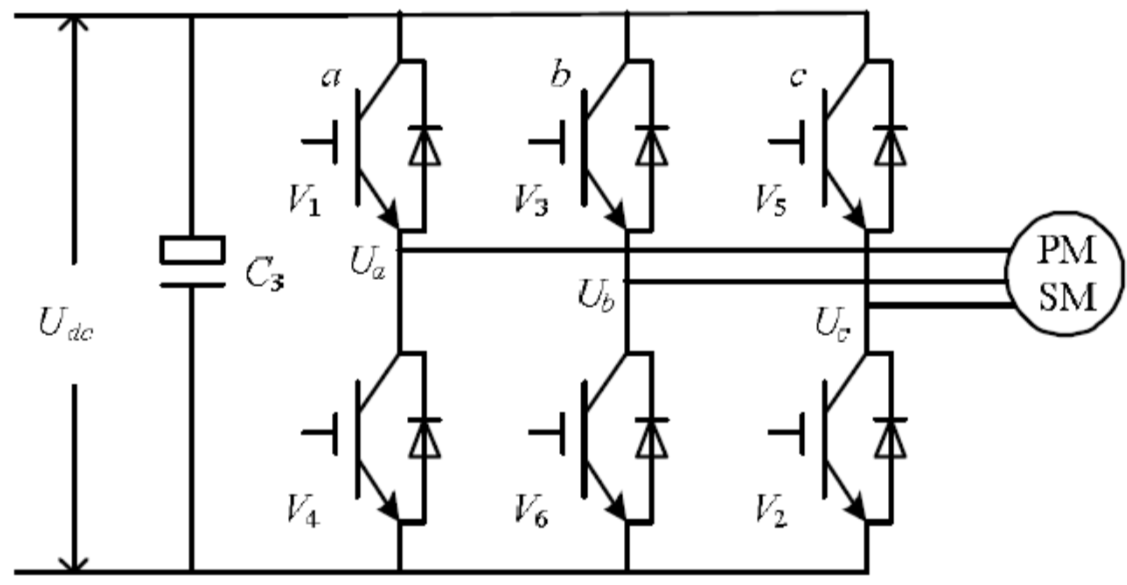
\includegraphics[width=0.4\textwidth]
    {图片/三相全桥逆变电路.png}
    \caption{三相全桥逆变电路}
    \label{fig:三相全桥逆变电路}
\end{figure}

SVPWM（Space Vector Pulse Width Modulation，空间矢量脉宽调制）
是一种针对三相全桥的PWM调制技术，其基本思想是将希望得到的电压矢量用多个基本矢量
来合成。基本矢量可以用\(U_{\mathrm{x}}(S_{\mathrm{A}},S_{\mathrm{B}}, S_{\mathrm{C}})\)表示，其中\(S_{\mathrm{A}},S_{\mathrm{B}},S_{\mathrm{C}}\)为三相全桥的
开关状态，而\(x=4S_{\mathrm{A}}+2S_{\mathrm{B}}+S_{\mathrm{C}}\)为基本矢量的索引。
如A相导通，B、C相截止，就可以表示为\(U_4(1,0,0)\)。

根据三相全桥各相的开关状态，基本矢量可以分为两种有效矢量和两种零矢量共四类。

第一种有效矢量包括\(U_4(1,0,0),U_2(0,1,0),U_1(0,0,1)\)三个基本矢量，特点是单相
上桥导通、两相下桥截止。此时导通的上桥流过的电流就是母线电流。

第二种有效矢量包括\(U_3(0,1,1),U_5(1,0,1),U_6(1,1,0)\)三个基本矢量，特点是两相
上桥导通、一相下桥截止。此时导通的下桥流过的电流就是母线电流。

另外还有两种零矢量为\(U_0(0,0,0)\)和\(U_7(1,1,1)\)，分别是三相截止和三相导通。
此时通过MOSFET、IGBT等功率器件的寄生/续流二极管形成环流。

将上述的基本矢量在两相静止坐标系种表示如下图所示。可以发现，平面被八个基本电压
矢量分割为了六个扇区。
\begin{figure}[H]
    \centering
    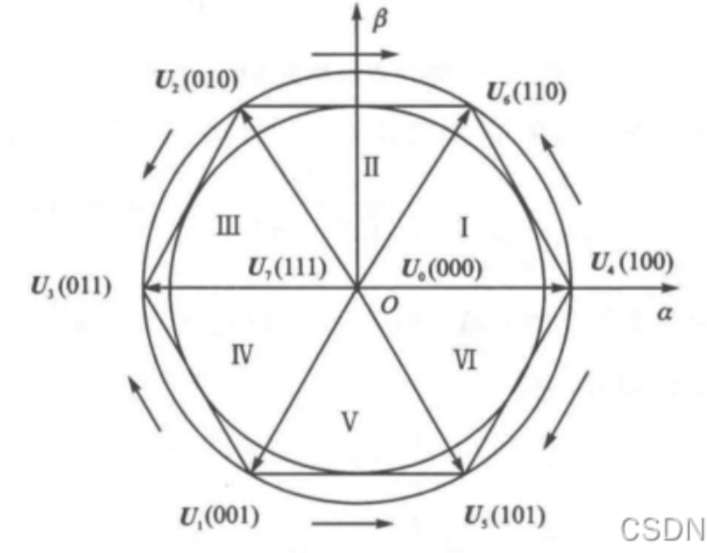
\includegraphics[width=0.6\textwidth]
    {图片/SVPWM基本矢量和扇区划分图.png}
·    \caption{SVPWM基本矢量和扇区划分图}
    \label{fig:SVPWM基本矢量和扇区划分图}
\end{figure}

根据等幅值克拉克变换\eqref{eq:克拉克变换}可得基本矢量幅值为
\(\cfrac{2}{3}U_{\mathrm{dc}}\)。
根据合成矢量的规则，任一电压矢量都可以用相邻60°的两个基本矢量和零矢量得到

接下来以第I扇区为例，讨论合成矢量的幅值要求。第I扇区可以使用有效矢量
\(U_4(1,0,0)\)和\(U_6(1,1,0)\)与零矢量\(U_0(0,0,0)\)和\(U_7(1,1,1)\)。
为了获取最大的电压矢量，假设零矢量不参与合成。在一个PWM周期内，\(k\)时间占比
由\(U_4(1,0,0)\)作用，而\(1-k\)时间占比由\(U_6(1,1,0)\)作用。

用复数表示合成矢量，则合成矢量可以表示为
\(U=\cfrac{2}{3}U_{\mathrm{dc}}(k+\cfrac 12(1-k)+\mathrm{j}\cfrac{\sqrt{3}}{2}(1-k))\)
，其中j表示虚数单位。该合成矢量的幅值为
\(\cfrac{2}{3}U_{\mathrm{dc}}\sqrt{(k+\cfrac 12-\cfrac 12k)^2+\cfrac 34(1-k)^2}
=\cfrac 23U_{\mathrm{dc}}\sqrt{k^2-k+1}\)
，其中作用时间占比\(k\in [0,1]\)。

根据二次函数相关知识可得当\(k=\cfrac 12\)时合成矢量幅值最小，此时合成矢量
幅值为\(\cfrac{1}{\sqrt 3}U_{\mathrm{dc}}\)。这就是可以完成线性调制的SVPWM电压极限圆
半径（正六边形内切圆）。在电压极限圆内，任何电压矢量都可以用基本矢量合成得到。
而超出电压极限圆范围，但只要处于正六边形范围内，也都可以用基本矢量合成得到。

由于正六边形范围的判断较为复杂，因此一般认为SVPWM的调制极限就是电压极限圆，
也即满足
\begin{equation}
    U_{\mathrm{d}}^2+U_{\mathrm{q}}^2\le \cfrac{U_{\mathrm{dc}}^2}{3}
    \label{eq:SVPWM电压极限圆}
\end{equation}

根据电压极限圆可知，SVPWM调制法的相电压最大利用率为
\(\cfrac{\frac{U_{\mathrm{dc}}}{\sqrt 3}}{U_{\mathrm{dc}}}\times100\%=57.7\%\)，
而线电压最大利用率为
\(\sqrt{3}\times \cfrac{\frac{U_{\mathrm{dc}}}{\sqrt 3}}{U_{\mathrm{dc}}}
\times100\%= 100\%\)。

\subsection{SVPWM调制法}
\label{sec:SVPWM调制法}

SVPWM调制法是基本的SVPWM实现方法，其物理含义直观，但是程序运行效率较低，
这是因为需要经过扇区判断、基本矢量作用时间计算、三相占空比计算三个步骤。

扇区判断的主要任务是，将给定的\(U_{\mathrm{d}},U_{\mathrm{q}}\)，通过\eqref{eq:帕克逆变换}的帕克
逆变换公式得到两相静止坐标系下的\(U_{\mathrm{\alpha}},U_{\mathrm{\beta}}\)，判断合成矢量
所在的扇区。

根据基本矢量图\ref{fig:SVPWM基本矢量和扇区划分图}，可以得到合成矢量
落在特定扇区的充要条件。
\begin{itemize}
    \item 
    扇区I：\(U_{\mathrm{\alpha}}>0,{U_{\mathrm{\beta}}>0},
    |\cfrac{U_{\mathrm{\beta}}}{U_{\mathrm{\alpha}}}|<\sqrt 3\)
    第三个条件也可以写为
    \(\begin{cases}\cfrac 12(\sqrt{3}U_{\mathrm{\alpha}}-U_{\mathrm{\beta}})>0\\
        \cfrac 12(-\sqrt{3}U_{\mathrm{\alpha}}-U_{\mathrm{\beta}})<0\end{cases}\)
    \item 
    扇区II：\({U_{\mathrm{\beta}}>0},|\cfrac{U_{\mathrm{\beta}}}{U_{\mathrm{\alpha}}}|>\sqrt 3\)
    第三个条件也可以写为
    \(\begin{cases}\cfrac 12(\sqrt{3}U_{\mathrm{\alpha}}-U_{\mathrm{\beta}})<0\\
        \cfrac 12(-\sqrt{3}U_{\mathrm{\alpha}}-U_{\mathrm{\beta}})<0\end{cases}\)
    \item 
    扇区III：\(U_{\mathrm{\alpha}}<0,{U_{\mathrm{\beta}}>0},
    |\cfrac{U_{\mathrm{\beta}}}{U_{\mathrm{\alpha}}}|<\sqrt 3\)
    第三个条件也可以写为
    \(\begin{cases}\cfrac 12(\sqrt{3}U_{\mathrm{\alpha}}-U_{\mathrm{\beta}})<0\\
        \cfrac 12(-\sqrt{3}U_{\mathrm{\alpha}}-U_{\mathrm{\beta}})>0\end{cases}\)
    \item 
    扇区IV：\(U_{\mathrm{\alpha}}<0,{U_{\mathrm{\beta}}<0},
    |\cfrac{U_{\mathrm{\beta}}}{U_{\mathrm{\alpha}}}|<\sqrt 3\)
    第三个条件也可以写为
    \(\begin{cases}\cfrac 12(\sqrt{3}U_{\mathrm{\alpha}}-U_{\mathrm{\beta}})<0\\
        \cfrac 12(-\sqrt{3}U_{\mathrm{\alpha}}-U_{\mathrm{\beta}})>0\end{cases}\)
    \item 
    扇区V：\({U_{\mathrm{\beta}}<0},|\cfrac{U_{\mathrm{\beta}}}{U_{\mathrm{\alpha}}}|>\sqrt 3\)
    第三个条件也可以写为
    \(\begin{cases}\cfrac 12(\sqrt{3}U_{\mathrm{\alpha}}-U_{\mathrm{\beta}})>0\\
        \cfrac 12(-\sqrt{3}U_{\mathrm{\alpha}}-U_{\mathrm{\beta}})>0\end{cases}\)
    \item 
    扇区VI：\(U_{\mathrm{\alpha}}>0,{U_{\mathrm{\beta}}<0},
    |\cfrac{U_{\mathrm{\beta}}}{U_{\mathrm{\alpha}}}|<\sqrt 3\)
    第三个条件也可以写为
    \(\begin{cases}\cfrac 12(\sqrt{3}U_{\mathrm{\alpha}}-U_{\mathrm{\beta}})>0\\
        \cfrac 12(-\sqrt{3}U_{\mathrm{\alpha}}-U_{\mathrm{\beta}})<0\end{cases}\)
\end{itemize}

可以发现上述条件判断都可以用
\(\begin{cases}A_0=U_{\mathrm{\beta}}
    \\A_1=\cfrac{\sqrt{3}}2U_{\mathrm{\alpha}}-\cfrac{1}{2}U_{\mathrm{\beta}}
    \\A_2=-\cfrac{\sqrt{3}}2U_{\mathrm{\alpha}}-\cfrac 12U_{\mathrm{\beta}}
\end{cases}\)
的符号判断来概括。若定义上述判断式结果大于零为真（1），小于零为假（0），
也就是满足\(X_i=\begin{cases}1&A_i>0\\0&A_i<0\end{cases}\)
则可以定义逻辑向量\((X_2,X_1,X_0)\)，索引值为\(N'=4X_2+2X_1+X_0\)。索引值的
可取值为\(1,2,3,4,5,6\)，分别对应六种扇区，记扇区号为\(N\)，判断表如下。
\begin{table}[H]
    \centering
    \begin{tabular}{|c|c|c|c|}
        \hline
        扇区号N&充要条件&逻辑向量&索引值N'\\
        \hline
        I&
        \(\begin{cases}-\sqrt{3}U_{\mathrm{\alpha}}-U_{\mathrm{\beta}}<0\\
            \sqrt{3}U_{\mathrm{\alpha}}-U_{\mathrm{\beta}}>0\\
            U_{\mathrm{\beta}}>0\end{cases}\)&
        (0,1,1)&3\\
        \hline
        II&
        \(\begin{cases}-\sqrt{3}U_{\mathrm{\alpha}}-U_{\mathrm{\beta}}<0\\
            \sqrt{3}U_{\mathrm{\alpha}}-U_{\mathrm{\beta}}<0\\
            U_{\mathrm{\beta}}>0\end{cases}\)&
        (0,0,1)&1\\
        \hline
        III&
        \(\begin{cases}-\sqrt{3}U_{\mathrm{\alpha}}-U_{\mathrm{\beta}}>0\\
            \sqrt{3}U_{\mathrm{\alpha}}-U_{\mathrm{\beta}}<0
            \\U_{\mathrm{\beta}}>0\end{cases}\)&
        (1,0,1)&5\\
        \hline
        IV&
        \(\begin{cases}-\sqrt{3}U_{\mathrm{\alpha}}-U_{\mathrm{\beta}}>0\\
            \sqrt{3}U_{\mathrm{\alpha}}-U_{\mathrm{\beta}}<0\\
            U_{\mathrm{\beta}}<0\end{cases}\)&
        (1,0,0)&4\\
        \hline
        V&
        \(\begin{cases}-\sqrt{3}U_{\mathrm{\alpha}}-U_{\mathrm{\beta}}>0\\
            \sqrt{3}U_{\mathrm{\alpha}}-U_{\mathrm{\beta}}>0\\
            U_{\mathrm{\beta}}<0\end{cases}\)&
        (1,1,0)&6\\
        \hline
        VI&
        \(\begin{cases}-\sqrt{3}U_{\mathrm{\alpha}}-U_{\mathrm{\beta}}<0\\
            \sqrt{3}U_{\mathrm{\alpha}}-U_{\mathrm{\beta}}>0\\
            U_{\mathrm{\beta}}<0\end{cases}\)&
        (0,1,0)&2\\
        \hline
    \end{tabular}
    \caption{扇区判断表}
    \label{tab:扇区判断表}
\end{table}

接下来考虑基本矢量的作用时间计算。假设一个PWM周期为\(T_{\mathrm{s}}\)。用于合成
矢量的两个基本有效矢量分别\(V_{\mathrm{x}}\)（角度为\(\theta_k\)，作用时间\(T_{\mathrm{x}}\)）
和\(V_{\mathrm{y}}\)（角度为\(\theta_k+\cfrac{\pi}{3}\)，作用时间\(T_{\mathrm{y}}\)）。其余时间
\(T_0=T_{\mathrm{s}}-T_{\mathrm{x}}-T_{\mathrm{y}}\)为零矢量作用。

有效矢量在两相静止坐标系\(\alpha-\beta\)下的坐标可以表示为
\(V_{\mathrm{x}}=\cfrac{2}{3}U_{\mathrm{dc}}(\cos\theta_k,\sin\theta_k)\)和
\(V_{\mathrm{y}}=\cfrac{2}{3}U_{\mathrm{dc}}(\cos\theta_k+\cfrac{\pi}{3},
\sin\theta_k+\cfrac{\pi}{3})\)。
因此根据期望合成矢量的坐标\((U_{\mathrm{\alpha}},U_{\mathrm{\beta}})\)，可以列写得到方程
\begin{equation*}
    \begin{cases}
        U_{\mathrm{\alpha}}T_{\mathrm{s}}=\cfrac{2}{3}U_{\mathrm{dc}}(T_{\mathrm{x}}\cos\theta_k+
        T_{\mathrm{y}}\cos(\theta_k+\cfrac{\pi}{3}))
        \\U_{\mathrm{\beta}}T_{\mathrm{s}}=\cfrac{2}{3}U_{\mathrm{dc}}(T_{\mathrm{x}}\sin\theta_k+
        T_{\mathrm{y}}\sin(\theta_k+\cfrac{\pi}{3}))
    \end{cases}
\end{equation*}

用矩阵可以表示为
\begin{equation*}
    \begin{bmatrix}
        \cos\theta_k&\cos(\theta_k+\cfrac{\pi}{3})\\
        \sin\theta_k&\sin(\theta_k+\cfrac{\pi}{3})
    \end{bmatrix}
    \begin{bmatrix}T_{\mathrm{x}}\\T_{\mathrm{y}}\end{bmatrix}
    =\cfrac{3T_{\mathrm{s}}}{2U_{\mathrm{dc}}}
    \begin{bmatrix}U_{\mathrm{\alpha}}\\U_{\mathrm{\beta}}\end{bmatrix}
\end{equation*}

方程的解为
\begin{equation*}
    \begin{bmatrix}T_{\mathrm{x}}\\T_{\mathrm{y}}\end{bmatrix}
    =
    \begin{bmatrix}
        \cos\theta_k&\cos(\theta_k+\cfrac{\pi}{3})\\
        \sin\theta_k&\sin(\theta_k+\cfrac{\pi}{3})
    \end{bmatrix}^{-1}
    \cfrac{3T_{\mathrm{s}}}{2U_{\mathrm{dc}}}
    \begin{bmatrix}U_{\mathrm{\alpha}}\\U_{\mathrm{\beta}}\end{bmatrix}
    =
    \cfrac{\sqrt 3T_{\mathrm{s}}}{U_{\mathrm{dc}}}
    \begin{bmatrix}
        \sin(\theta_k+\cfrac{\pi}{3})
        &-\cos(\theta_k+\cfrac{\pi}{3})\\
        -\sin\theta_k&\cos\theta_k
    \end{bmatrix}
    \begin{bmatrix}U_{\mathrm{\alpha}}\\U_{\mathrm{\beta}}\end{bmatrix}
\end{equation*}

上式中\(\theta_k\)中由扇区号\(N\)决定，即
\(\theta_k=(N-1)\times\cfrac{\pi}{3},N=1\sim6\)。并且在前述扇区判断过程中
已经定义了判断扇区用到的三个表达式 
\(\begin{cases}A_0=U_{\mathrm{\beta}}
    \\A_1=\cfrac{\sqrt{3}}2U_{\mathrm{\alpha}}-\cfrac{1}{2}U_{\mathrm{\beta}}
    \\A_2=-\cfrac{\sqrt{3}}2U_{\mathrm{\alpha}}-\cfrac 12U_{\mathrm{\beta}}
\end{cases}\)，
其也是简化计算基本矢量作用时间的核心。定义基本矢量作用时间系数为
\begin{equation*}
    K=\cfrac{\sqrt 3T_{\mathrm{s}}}{U_{\mathrm{dc}}}
\end{equation*}

那么各个扇区下作用时间可以通过查表实现：
\begin{table}[H]
    \centering
    \begin{tabular}{|c|c|c|}
        \hline
        扇区号N&作用时间\(T_{\mathrm{x}}\)&作用时间\(T_{\mathrm{y}}\)\\
        \hline
        I&\(KA_1\)&\(KA_0\)\\
        \hline
        II&\(-KA_2\)&\(-KA_1\)\\
        \hline
        III&\(KA_0\)&\(KA_2\)\\
        \hline
        IV&\(-KA_1\)&\(-KA_0\)\\
        \hline
        V&\(KA_2\)&\(KA_1\)\\
        \hline
        VI&\(-KA_0\)&\(-KA_2\)\\
        \hline
    \end{tabular}
    \caption{基本矢量作用时间计算表（\(T_{\mathrm{x}},T_{\mathrm{y}}\)表示）}
    \label{tab:基本矢量作用时间计算表(Tx,Ty表示)}
\end{table}

两个基本矢量\(V_{\mathrm{x}},V_{\mathrm{y}}\)的关系是\(V_{\mathrm{y}}\)总是超前\(V_{\mathrm{x}}\)60°。但在实际控制波形中
基本矢量的作用顺序为下式表示的七段式SVPWM：
\begin{equation*}
    U_0(0,0,0)\to
    \begin{cases}U_4(1,0,0)\\U_2(0,1,0)\\U_1(0,0,1)\end{cases}
    \to
    \begin{cases}U_6(1,1,0)\\U_5(1,0,1)\\U_3(0,1,1)\end{cases}
    \to
    U_7(1,1,1)
    \to
    \begin{cases}U_6(1,1,0)\\U_5(1,0,1)\\U_3(0,1,1)\end{cases}、
    \to
    \begin{cases}U_4(1,0,0)\\U_2(0,1,0)\\U_1(0,0,1)\end{cases}
    \to
    U_0(0,0,0)
\end{equation*}

也即总是单相上桥导通矢量先出现，两相上桥导通矢量后出现
因此根据各个扇区的\(V_{\mathrm{x}},V_{\mathrm{y}}\)与单相/两相上桥导通矢量的对应关系，可以将
表\ref{tab:基本矢量作用时间计算表(Tx,Ty表示)}中的基本矢量作用时
间\(T_{\mathrm{x}}\)和\(T_{\mathrm{y}}\)，改写为用单相上桥导通矢量作用时间\(T_{\mathrm{U1}}\)
和两相上桥导通矢量作用时间\(T_{\mathrm{U2}}\)表示的计算表
\ref{tab:基本矢量作用时间计算表(TU1,TU2表示)}。
\begin{table}[H]
    \centering
    \begin{tabular}{|c|c|c|}
        \hline
        扇区号N&作用时间\(T_{\mathrm{U1}}\)&作用时间\(T_{\mathrm{U2}}\)\\
        \hline
        I&\(KA_1\)&\(KA_0\)\\
        \hline
        II&\(-KA_1\)&\(-KA_0\)\\
        \hline
        III&\(KA_0\)&\(KA_2\)\\
        \hline
        IV&\(-KA_0\)&\(-KA_1\)\\
        \hline
        V&\(KA_2\)&\(KA_1\)\\
        \hline
        VI&\(-KA_2\)&\(-KA_1\)\\
        \hline
    \end{tabular}
    \caption{基本矢量作用时间计算表（\(T_{\mathrm{U1}},T_{\mathrm{U2}}\)表示）}
    \label{tab:基本矢量作用时间计算表(TU1,TU2表示)}
\end{table}

最后根据基本矢量作用时间表
\ref{tab:基本矢量作用时间计算表(TU1,TU2表示)}以及PWM周期\(T_{\mathrm{s}}\)，
可以得到零矢量作用时间\(T_0=T_{\mathrm{s}}-T_{\mathrm{U1}}-T_{\mathrm{U2}}\)。

接下来进行三相占空比的计算。以第I扇区为例，其参与合成的基本矢量为
\(U_4(1,0,0)\)，\(U_6(1,1,0)\)，\(U_0(0,0,0)\)和\(U_7(1,1,1)\)。
可以发现，在第I扇区，C相只参与零矢量合成，
B相参与两相上桥导通基本矢量和零矢量合成，
而A相参与单相、两相上桥导通基本矢量和零矢量的合成。
通过分析各个扇区内每一相的矢量合成参与情况，可以得到ABC三相在其中的角色。
因此只需要关注如何计算出：只参与零矢量合成相的占空比\(D_0\)、
参与两相上桥导通基本矢量和零矢量合成相的占空比\(D_1\)、
参与单相、两相上桥导通基本矢量和零矢量合成相的占空比\(D_2\)
三个占空比即可。

对于\(D_0\)，其导通时间就是\(U_7(1,1,1)\)的导通时间。而在七段式SVPWM中
\(U_7(1,1,1)\)的导通时间与\(U_0(0,0,0)\)的导通时间相同，均为\(\cfrac{1}{2}T_0\)
。考虑到PWM周期为\(T_{\mathrm{s}}\)，所以\(D_0=\cfrac{T_0}{2T_{\mathrm{s}}}\)。

对于\(D_1\)，相较于\(D_0\)相，多了两相上桥导通的作用时间。因此占空比有
\(D_1=D_0+\cfrac{T_{\mathrm{U2}}}{T_{\mathrm{s}}}\)。

对于\(D_2\)，相较于\(D_1\)相，多了单相上桥导通的作用时间。因此占空比有
\(D_2=D_1+\cfrac{T_{\mathrm{U1}}}{T_{\mathrm{s}}}\)。

最后根据每个扇区各相的参与情况，得到三相占空比计算表
\ref{tab:三相占空比计算表}。
\begin{table}[H]
    \centering
    \begin{tabular}{|c|c|c|c|}
        \hline
        扇区号N&A相占空比&B相占空比&C相占空比\\
        \hline
        I&\(D_2\)&\(D_1\)&\(D_0\)\\
        \hline
        II&\(D_1\)&\(D_2\)&\(D_0\)\\
        \hline
        III&\(D_0\)&\(D_2\)&\(D_1\)\\
        \hline
        IV&\(D_0\)&\(D_1\)&\(D_2\)\\
        \hline
        V&\(D_1\)&\(D_0\)&\(D_2\)\\
        \hline
        VI&\(D_2\)&\(D_0\)&\(D_1\)\\
        \hline
    \end{tabular}
    \caption{三相占空比计算表}
    \label{tab:三相占空比计算表}
\end{table}

综上所述，SVPWM调制法的步骤为：扇区判断（表\ref{tab:扇区判断表}）
、基本矢量作用时间计算（表\ref{tab:基本矢量作用时间计算表(TU1,TU2表示)}）
、三相占空比计算（表\ref{tab:三相占空比计算表}）三个步骤。期间需要大量查表
，程序执行较为繁琐。

\subsection{SVPWM计算法}

为了克服SVPWM调制法中需要大量查表的问题，可以从结果反推如何通过
计算的方法实现SVPWM调制。

在恒定电角速度情况下，取直流电压\(U_{\mathrm{dc}}=12V\)，期望
直轴电压\(U_{\mathrm{d}}=0V\)，交轴电压\(U_{\mathrm{q}}=3V\)确保位于电压极限圆，
则输出的三相电压（三相占空比乘直流电压）如下图\ref{fig:SVPWM电压}所示。
\begin{figure}[H]
    \centering
    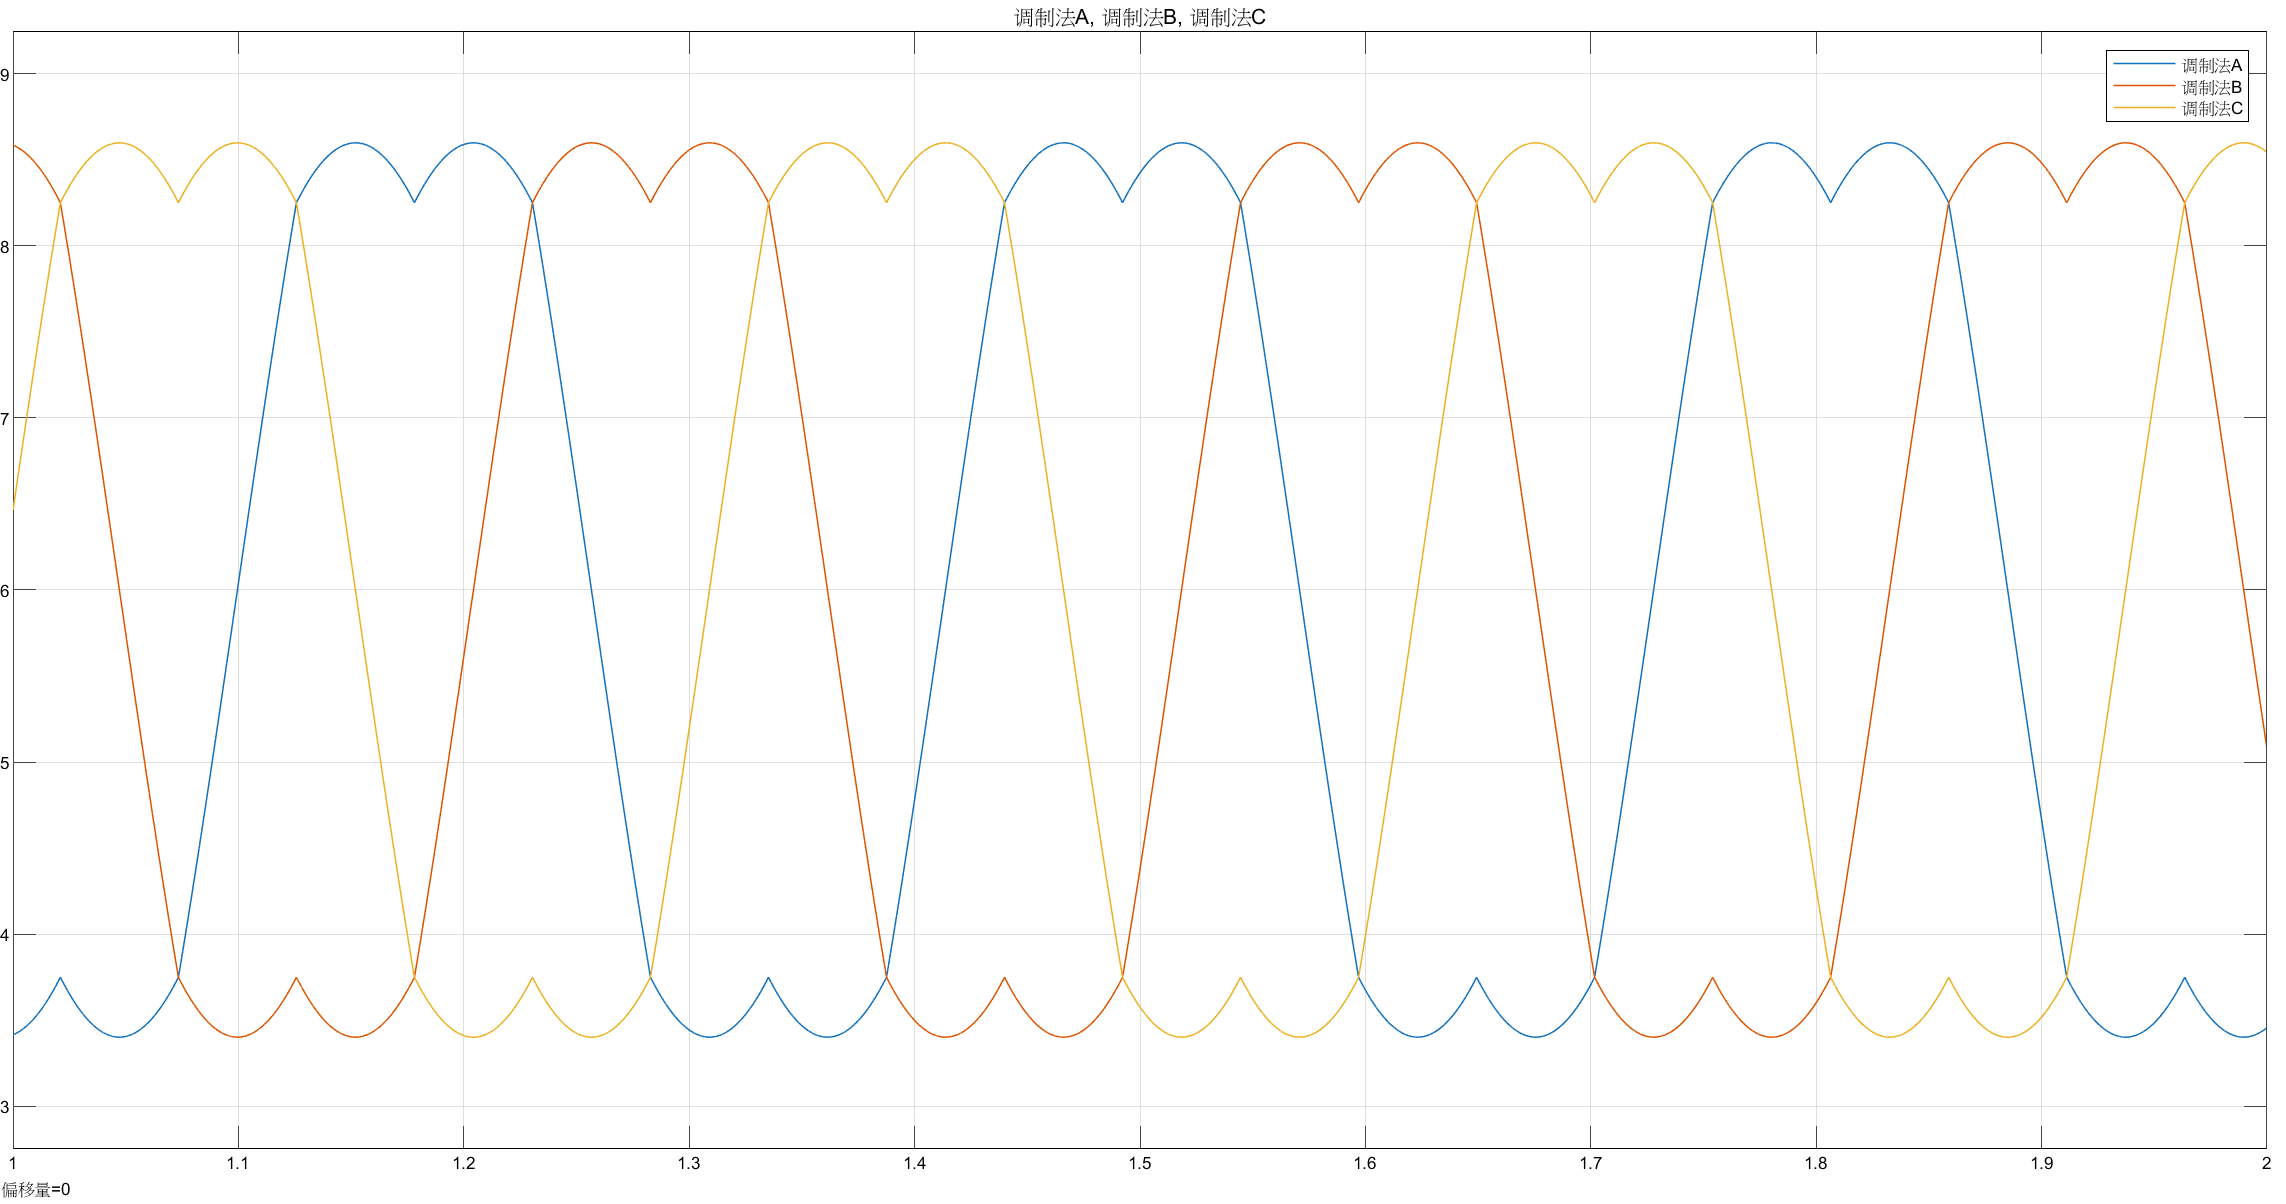
\includegraphics[width=0.8\textwidth]
    {图片/SVPWM电压波形.png}
    \caption{SVPWM电压波形}
    \label{fig:SVPWM电压}
\end{figure}

可以发现SVPWM波形为类马鞍波。若以SPWM调制的正弦波为基波，则SVPWM是在
正弦基波基础上叠加了一个基波频率为正弦基波频率三倍的波形。
为了便于观察，取A相电压波形，将直接通过克拉克-帕克逆变换的原始波形、
通过SVPWM调制后的相电压波形（去除直流分量）相比，并且用SVPWM调制波形
减去原始波形，观察注入波形的样式，
如下图\ref{fig:A相电压波形}所示。
\begin{figure}[H]
    \centering
    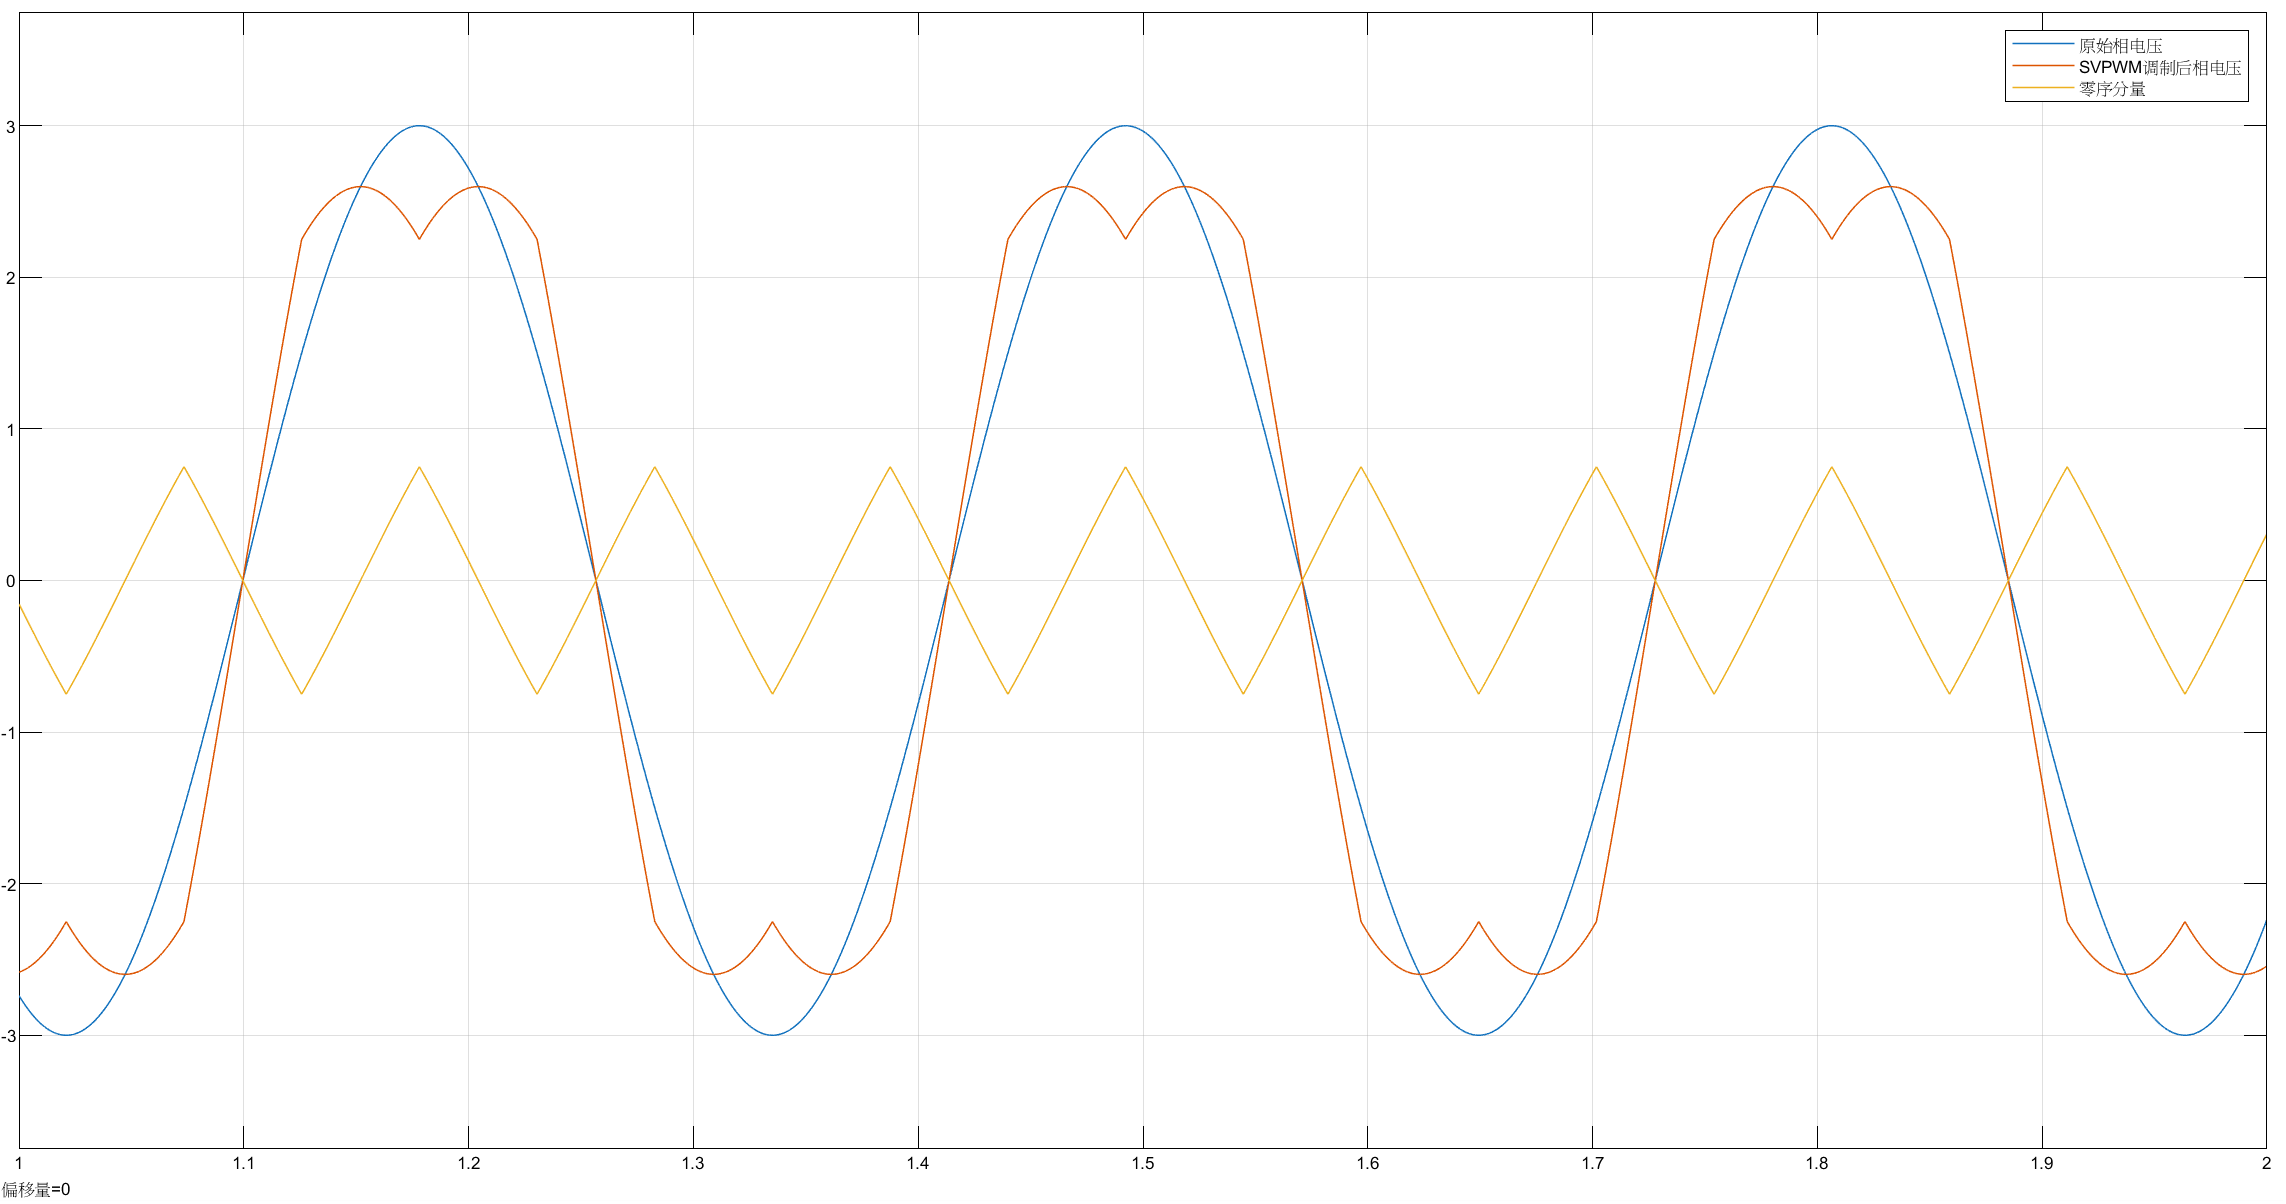
\includegraphics[width=0.8\textwidth]
    {图片/A相电压波形.png}
    \caption{A相电压波形}
    \label{fig:A相电压波形}
\end{figure}

SVPWM调制通过在基波基础上注入三倍频率的三角波实现了
电压利用率的提高，这是SVPWM电压利用率远超SPWM的关键所在。
由于该三角波在相电压中注入且基波频率恰好是正弦波频率的三倍，
因此在线电压中会相互抵消，使得线电压波形仍为正弦波。
由于该三角波注入没有影响线电压谐波，所以将该三角波称为零序分量。

零序分量\(U_{\mathrm{0}}\)与克拉克-帕克逆变换得到的三相电压波形如下图
\ref{fig:原始相电压波形与零序分量波形}所示。
可以发现，零序分量在自然换相点达到极值，在任意一相过零点归零，
并且全程线性变化。
\begin{figure}[H]
    \centering
    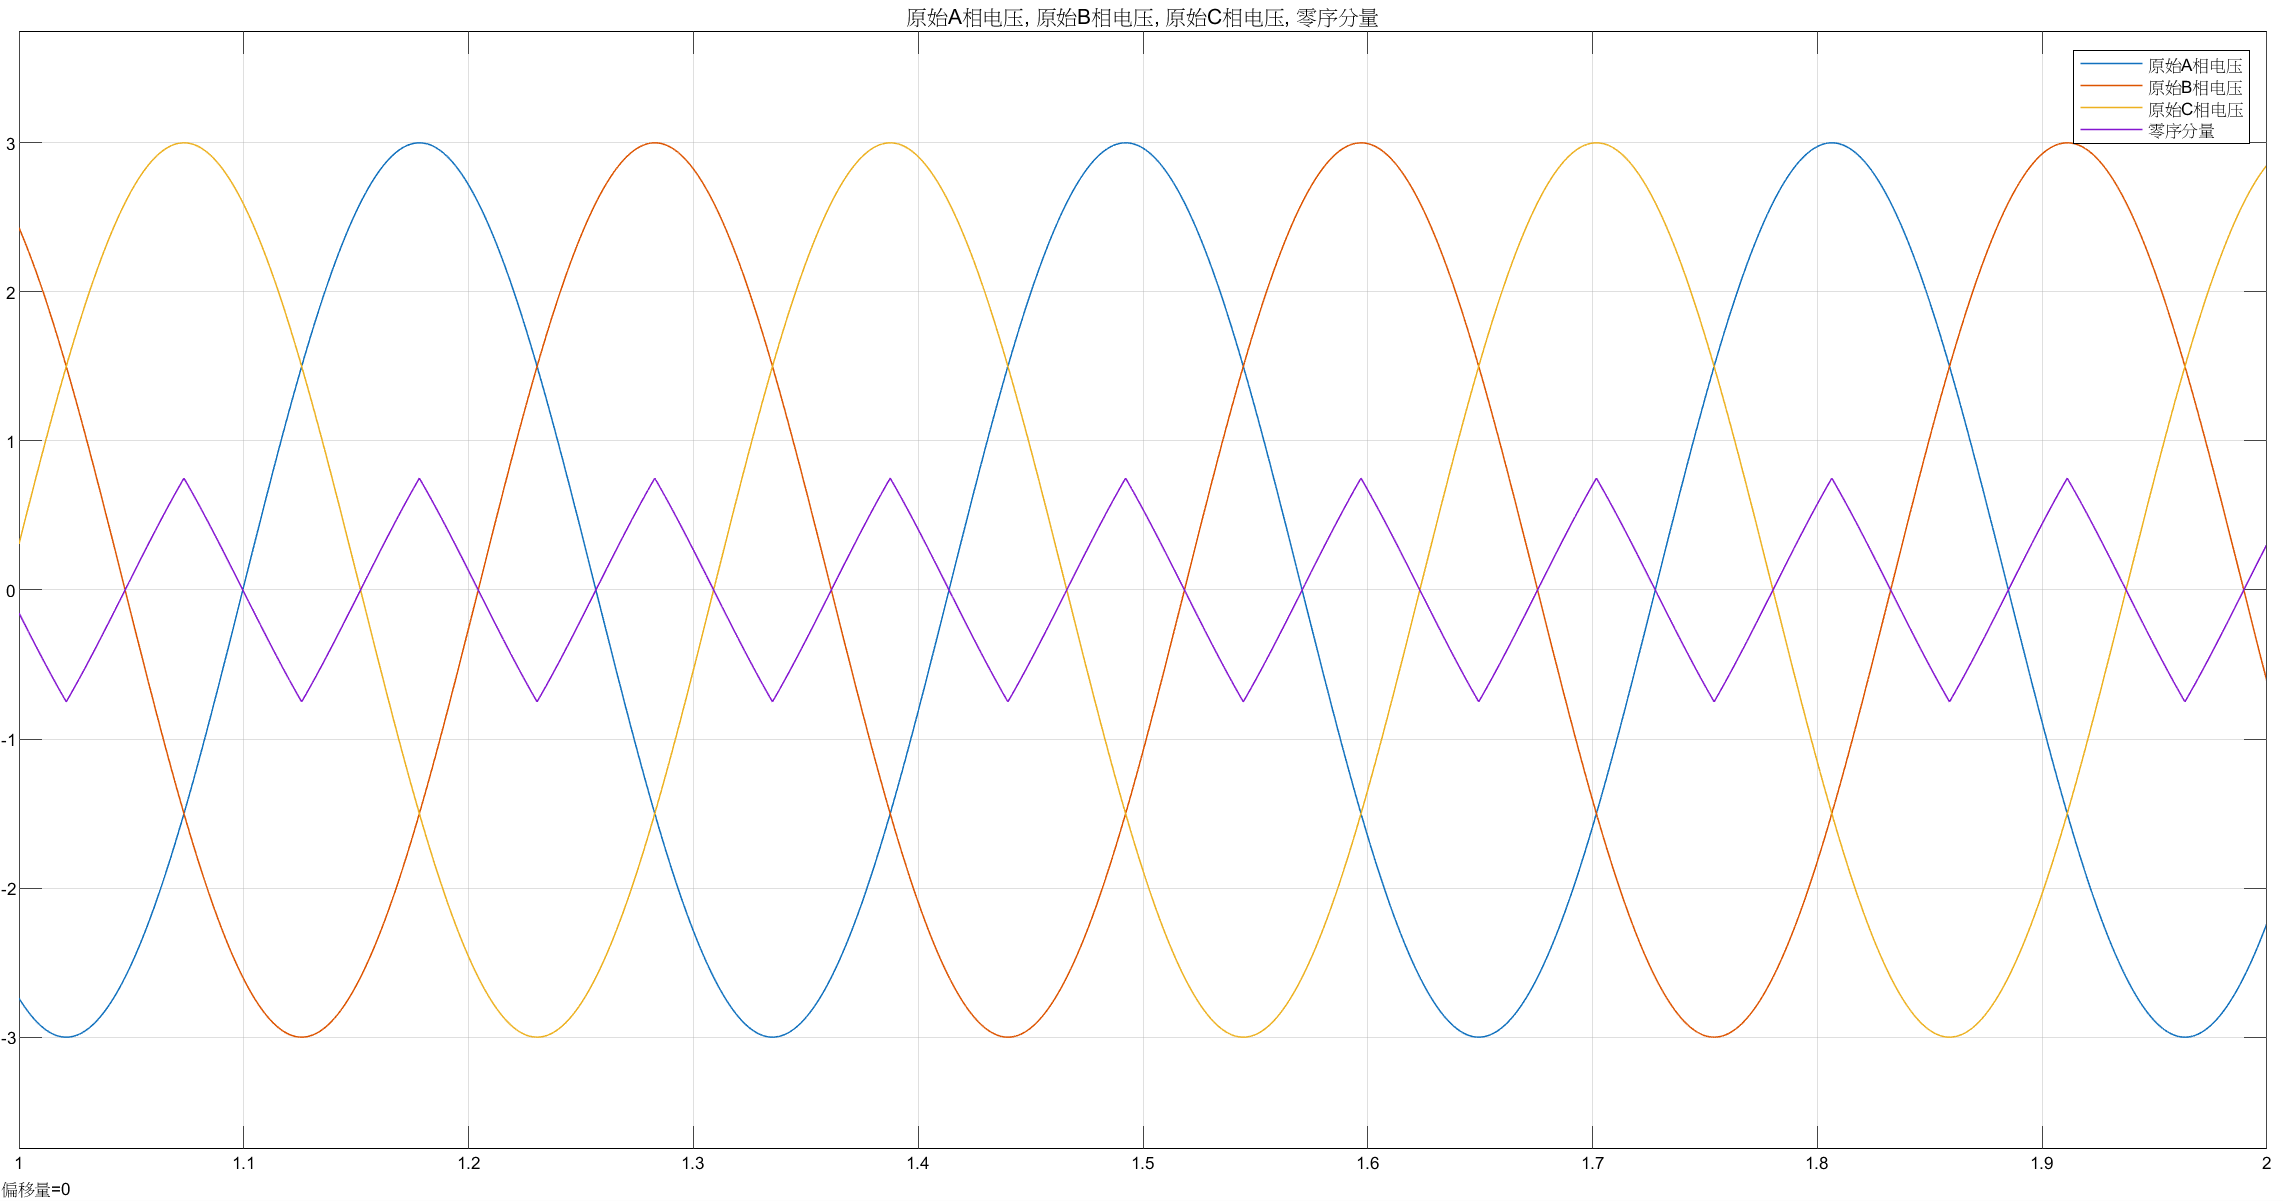
\includegraphics[width=0.8\textwidth]
    {图片/原始相电压波形与零序分量波形.png}
    \caption{原始相电压波形与零序分量波形}
    \label{fig:原始相电压波形与零序分量波形}
\end{figure}

设期望的\(U_{\mathrm{d}},U_{\mathrm{q}}\)经过克拉克-帕克逆变换得到的三相原始相电压为
\(U_{\mathrm{a}},U_{\mathrm{b}},U_{\mathrm{c}}\)。
注入零序分量\(U_{\mathrm{0}}\)后，调制相电压为：
\begin{equation}
    \begin{cases}
        U_{\mathrm{a}}' = U_{\mathrm{a}} + U_{\mathrm{0}}\\
        U_{\mathrm{b}}' = U_{\mathrm{b}} + U_{\mathrm{0}}\\
        U_{\mathrm{c}}' = U_{\mathrm{c}} + U_{\mathrm{0}}   
    \end{cases}
    \label{eq:注入后相电压}
\end{equation}

可以发现，零序分量注入前后线电压维持恒定：
\begin{equation*}
    \begin{cases}
        U_{\mathrm{ab}}' = U_{\mathrm{a}}' - U_{\mathrm{b}}'
        = U_{\mathrm{a}} - U_{\mathrm{b}} = U_{\mathrm{ab}}\\
        U_{\mathrm{bc}}' = U_{\mathrm{b}}' - U_{\mathrm{c}}'
        = U_{\mathrm{b}} - U_{\mathrm{c}} = U_{\mathrm{bc}}\\
        U_{\mathrm{ca}}' = U_{\mathrm{c}}' - U_{\mathrm{a}}'
        = U_{\mathrm{c}} - U_{\mathrm{a}} = U_{\mathrm{ca}}
    \end{cases}
\end{equation*}

因此无论\(U_{\mathrm{0}}\)取何值，线电压波形始终保持不变。
也就是说，在线性调制的前提下，零序分量注入与否不影响实际的电机运行
\footnote{电机运行主要取决于线电压而不是相电压。}。但零序分量注入后，
相同线电压需要的相电压幅值降低，相当于扩大了线性调制区间。
为保证线性调制（不进入过调制区），调制后的三相相电压必须限制在
直流母线电压范围内：
\begin{equation*}
    -\cfrac{U_{\mathrm{dc}}}{2} \le U_{\mathrm{a}}',U_{\mathrm{b}}',U_{\mathrm{c}}'
    \le \cfrac{U_{\mathrm{dc}}}{2}
\end{equation*}

记三相原始电压的最大值和最小值分别为
\begin{equation*}
    \begin{cases}
        U_{\mathrm{\max}} = \max(U_{\mathrm{a}},U_{\mathrm{b}},U_{\mathrm{c}})\\
        U_{\mathrm{\min}} = \min(U_{\mathrm{a}},U_{\mathrm{b}},U_{\mathrm{c}})
    \end{cases}
\end{equation*}

则上述电压范围约束等价于对调制后最大相电压和最小相电压的要求：
\begin{equation*}
    \begin{cases}
        U_{\mathrm{\min}} + U_{\mathrm{0}} \ge -\cfrac{U_{\mathrm{dc}}}{2}\\[8pt]
        U_{\mathrm{\max}} + U_{\mathrm{0}} \le \cfrac{U_{\mathrm{dc}}}{2}
    \end{cases}
\end{equation*}

满足上式的\(U_{\mathrm{0}}\)有无穷多个，
而SVPWM选择的策略为居中对称，
令调制后最大相电压到上边界的电压裕量\(\cfrac{U_{\mathrm{dc}}}{2}-(U_{\mathrm{\max}}+U_{\mathrm{0}})\)
与最小相电压到下边界的电压裕量\((U_{\mathrm{\min}}+U_{\mathrm{0}})-(-\cfrac{U_{\mathrm{dc}}}{2})\)
保持相等，即：
\begin{equation*}
    \cfrac{U_{\mathrm{dc}}}{2} - (U_{\mathrm{\max}} + U_{\mathrm{0}})
    = (U_{\mathrm{\min}} + U_{\mathrm{0}}) + \cfrac{U_{\mathrm{dc}}}{2}
\end{equation*}

化简得：
\begin{equation}
    U_{\mathrm{0}} = -\cfrac{1}{2}(U_{\mathrm{\max}} + U_{\mathrm{\min}})
    \label{eq:零序分量表达式}
\end{equation}

因此就可以得到计算法的三相占空比表达式：
\begin{equation}
    \begin{cases}
        D_{\mathrm{A}} = \cfrac{1}{2} +\cfrac{U_{\mathrm{0}}+U_{\mathrm{a}}}{U_{\mathrm{dc}}}\\
        D_{\mathrm{B}} = \cfrac{1}{2} +\cfrac{U_{\mathrm{0}}+U_{\mathrm{b}}}{U_{\mathrm{dc}}}\\
        D_{\mathrm{C}} = \cfrac{1}{2} +\cfrac{U_{\mathrm{0}}+U_{\mathrm{c}}}{U_{\mathrm{dc}}}
    \end{cases}
    \label{eq:三相占空比表达式}
\end{equation}

式\eqref{eq:零序分量表达式}即为SVPWM零序分量的解析表达式。相关的波形示意如下图所示。
\begin{figure}[H]
    \centering
    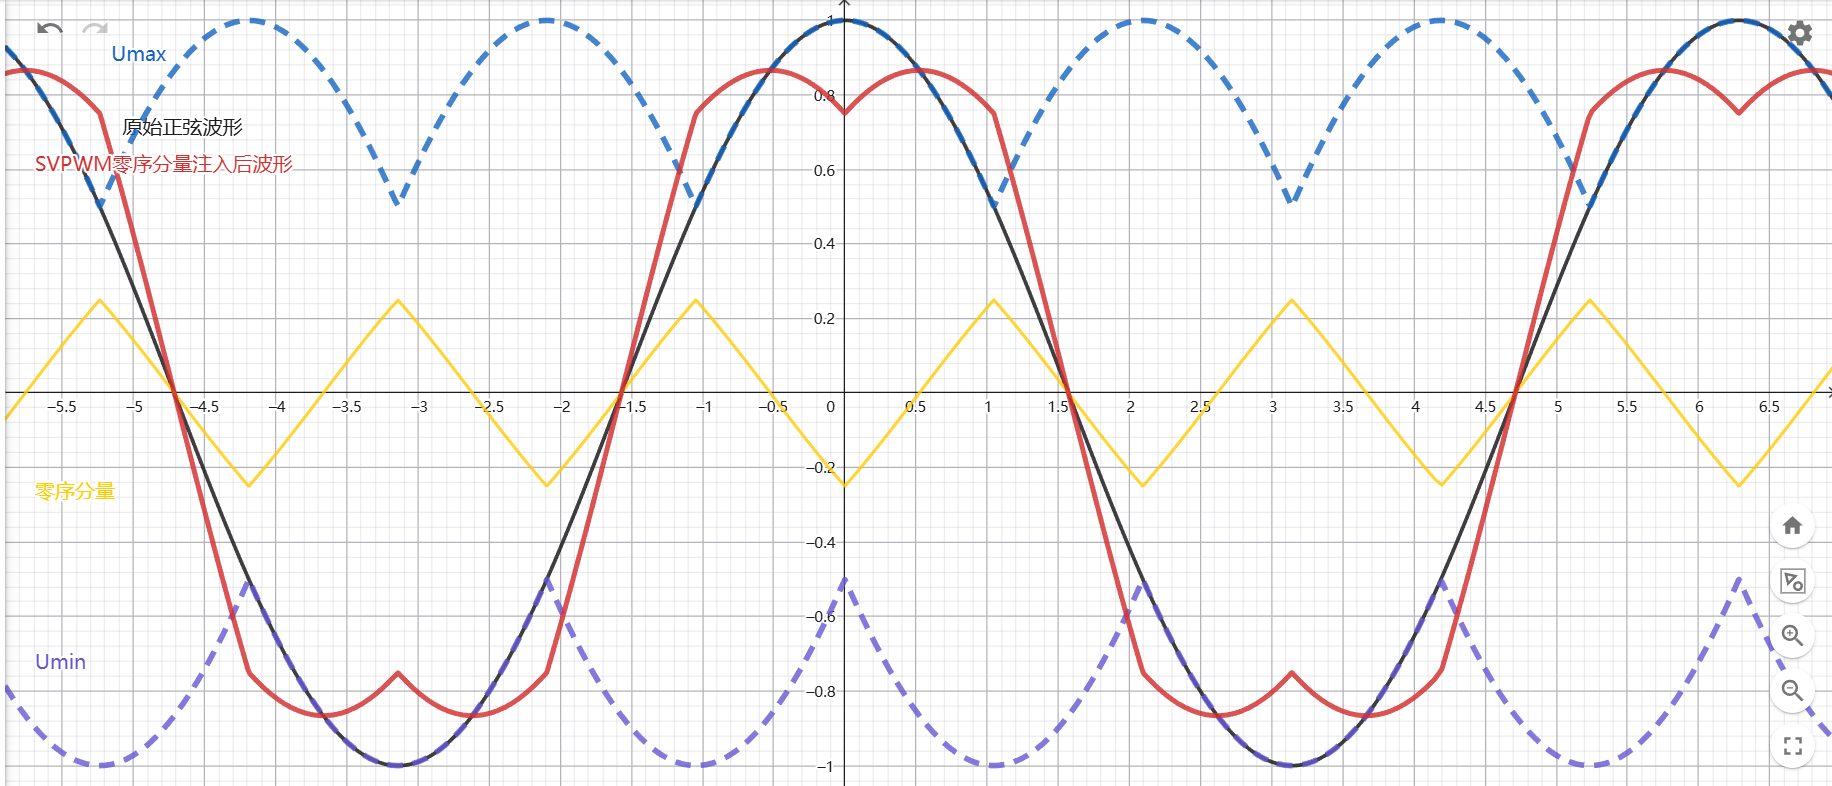
\includegraphics[width=0.8\textwidth]
    {图片/零序分量计算相关波形.png}
    \caption{零序分量计算相关波形示意}
    \label{fig:零序分量计算相关波形示意}
\end{figure}

接下来以第I扇区为例，证明\eqref{eq:零序分量表达式}零序分量注入的结果与第\ref{sec:SVPWM调制法}节中给出的调制法结果一致。
根据调制法中间步骤，中间变量满足：
\begin{equation*}
    \begin{cases}
        A_0 = U_{\mathrm{\beta}}\\
        A_1 = \cfrac{\sqrt{3}}{2}U_{\mathrm{\alpha}} - \cfrac{1}{2}U_{\mathrm{\beta}}\\
        A_2 = -\cfrac{\sqrt{3}}{2}U_{\mathrm{\alpha}} - \cfrac{1}{2}U_{\mathrm{\beta}}\\
        K = \cfrac{\sqrt{3}T_{\mathrm{s}}}{U_{\mathrm{dc}}}
    \end{cases}
\end{equation*}

由表\ref{tab:基本矢量作用时间计算表(TU1,TU2表示)}可知，
第I扇区有\(T_{\mathrm{U1}} = KA_1\)，\(T_{\mathrm{U2}} = KA_0\)，
而\(T_0=T_{\mathrm{s}}-T_{\mathrm{U1}}-T_{\mathrm{U2}}\)，
代入占空比定义可得：
\begin{equation*}
    \begin{cases}
        D_0=\cfrac{T_0}{2T_{\mathrm{s}}}=\cfrac{1}{2}(1-\cfrac{\sqrt{3}A_1}{U_{\mathrm{dc}}}
        -\cfrac{\sqrt{3}A_0}{U_{\mathrm{dc}}})\\
        D_1=D_0+\cfrac{T_{\mathrm{U2}}}{T_{\mathrm{s}}}=\cfrac{1}{2}(1-\cfrac{\sqrt{3}A_1}{U_{\mathrm{dc}}}
        +\cfrac{\sqrt{3}A_0}{U_{\mathrm{dc}}})\\
        D_2=D_1+\cfrac{T_{\mathrm{U1}}}{T_{\mathrm{s}}}=\cfrac{1}{2}(1+\cfrac{\sqrt{3}A_1}{U_{\mathrm{dc}}}
        +\cfrac{\sqrt{3}A_0}{U_{\mathrm{dc}}})
    \end{cases}
\end{equation*}

由表\ref{tab:三相占空比计算表}，第I扇区三相占空比分配为
A相\(D_2\)、B相\(D_1\)、C相\(D_0\)。
相较于虚拟中性点\(\cfrac{1}{2}U_{\mathrm{dc}}\)的调制相电压由占空比决定：
\begin{equation*}
    \begin{cases}
        U_{\mathrm{a,M}}' = (D_{\mathrm{A}}-\cfrac{1}{2})U_{\mathrm{dc}}=(D_{2}-\cfrac{1}{2})U_{\mathrm{dc}}
        =\cfrac{\sqrt{3}}{2}(A_0 + A_1)\\
        U_{\mathrm{b,M}}' = (D_{\mathrm{B}}-\cfrac{1}{2})U_{\mathrm{dc}}=(D_{1}-\cfrac{1}{2})U_{\mathrm{dc}}
        =\cfrac{\sqrt{3}}{2}(A_0 - A_1)\\
        U_{\mathrm{c,M}}' = (D_{\mathrm{C}}-\cfrac{1}{2})U_{\mathrm{dc}}=(D_{0}-\cfrac{1}{2})U_{\mathrm{dc}}
        =\cfrac{\sqrt{3}}{2}(-A_0 - A_1)
    \end{cases}
\end{equation*}

另一边，根据克拉克变换\eqref{eq:克拉克变换}，原始三相电压可以用逻辑向量\(A_0,A_1\)表示为：
\begin{equation*}
    \begin{cases}
        U_{\mathrm{a}} = U_{\mathrm{\alpha}}
        = \cfrac{1}{\sqrt{3}}(2A_1 + A_0)\\
        U_{\mathrm{b}} = -\cfrac{1}{2}U_{\mathrm{\alpha}} + \cfrac{\sqrt{3}}{2}U_{\mathrm{\beta}}
        = \cfrac{1}{\sqrt{3}}(A_0-A_1)\\
        U_{\mathrm{c}} = -\cfrac{1}{2}U_{\mathrm{\alpha}} - \cfrac{\sqrt{3}}{2}U_{\mathrm{\beta}}
        = \cfrac{1}{\sqrt{3}}(-A_1-2A_0)
    \end{cases}
\end{equation*}

在第I扇区，由扇区判断条件易知\(U_{\mathrm{a}}>U_{\mathrm{b}}>U_{\mathrm{c}}\)，
即\(U_{\mathrm{\max}}=U_{\mathrm{a}}\)，\(U_{\mathrm{\min}}=U_{\mathrm{c}}\)。
将上式代入零序分量公式
\eqref{eq:零序分量表达式}可得：
\begin{equation*}
    U_{\mathrm{0}} = -\cfrac{U_{\mathrm{a}} + U_{\mathrm{c}}}{2} = \cfrac{1}{2\sqrt{3}}(A_0-A_1)
\end{equation*}

将原始相电压与零序分量叠加，得到计算法在第I扇区的调制相电压：
\begin{equation*}
    \begin{cases}
        U_{\mathrm{a,C}}'=U_{\mathrm{a}}+U_{\mathrm{0}}
        =\cfrac{1}{2\sqrt{3}}(3A_1+3A_0)=\cfrac{\sqrt{3}}{2}(A_0 + A_1)=U_{\mathrm{a,M}}'\\
        U_{\mathrm{b,C}}'=U_{\mathrm{b}}+U_{\mathrm{0}}
        =\cfrac{1}{2\sqrt{3}}(3A_0-3A_1)=\cfrac{\sqrt{3}}{2}(A_0 - A_1)=U_{\mathrm{b,M}}'\\
        U_{\mathrm{c,C}}'=U_{\mathrm{c}}+U_{\mathrm{0}} 
        =\cfrac{1}{2\sqrt{3}}(-3A_1-3A_0)=\cfrac{\sqrt{3}}{2}(-A_0 - A_1)=U_{\mathrm{c,M}}'\\
    \end{cases}
\end{equation*}

可以发现调制法和计算法结果一致。其余五个扇区证明同理。通过SVPWM计算法，大大省略了调制法需要的查表运算，无需
程序分支，只需要按照公式\eqref{eq:零序分量表达式}
和\eqref{eq:三相占空比表达式}计算即可，更加适合实时控制场合。


\newpage
\section{经典FOC的速度-电流双闭环PI控制实现}

经典的FOC速度-电流双闭环PI控制系统框图如下图所示。
\begin{figure}[H]
    \centering
    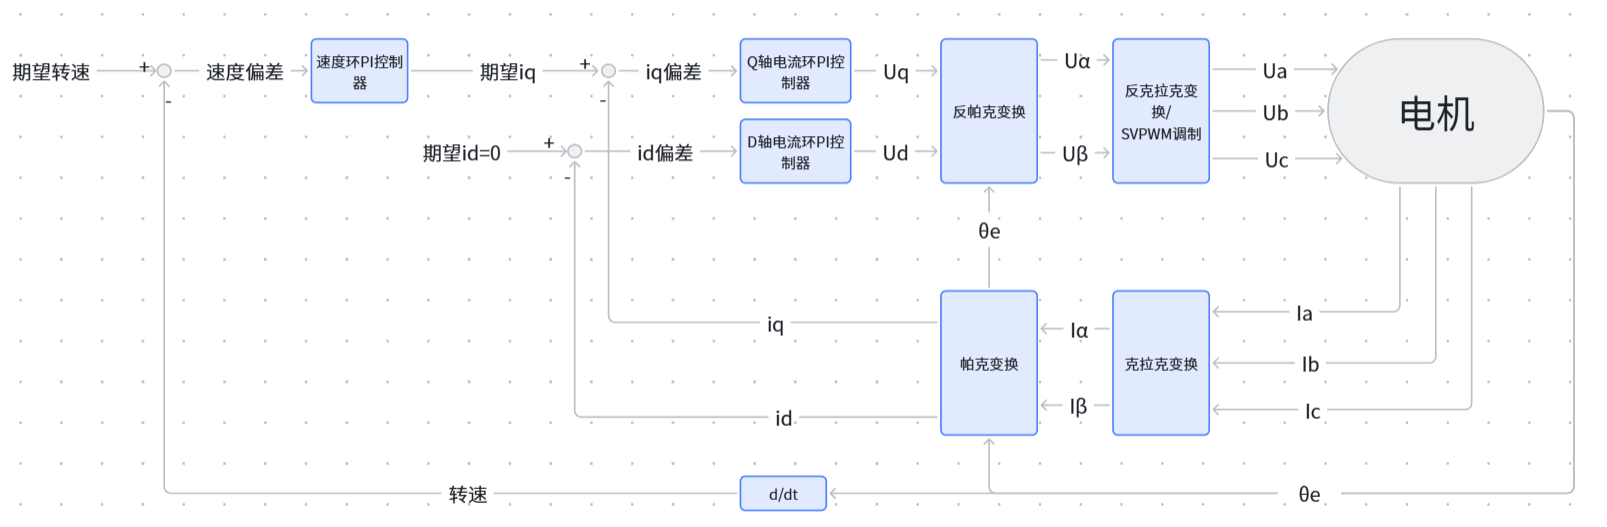
\includegraphics[width=0.8\textwidth]
    {图片/经典FOC控制结构框图.png}
    \caption{经典FOC控制结构框图}
    \label{fig:经典FOC控制结构框图}
\end{figure}
接下来将逐个介绍每个模块的实现。

\subsection{硬件设计}
一个完整的FOC控制系统硬件部分主要由以下几部分组成：主控MCU、电流传感器、转子位置传感器（编码器）、三相全桥驱动器、三相全桥电路、电源电路
、其他设备（如通信接口等）。

对于主控MCU，采用意法半导体的STMG431CBU6。其主频可达170MHz，并且支持DSP库，是意法半导体为电机驱动与控制而做了专门适配的微控制器。
开发过程中先使用核心板进行调试，相关电路如下图\ref{fig:核心板电路}所示。
\begin{figure}[H]
    \centering
    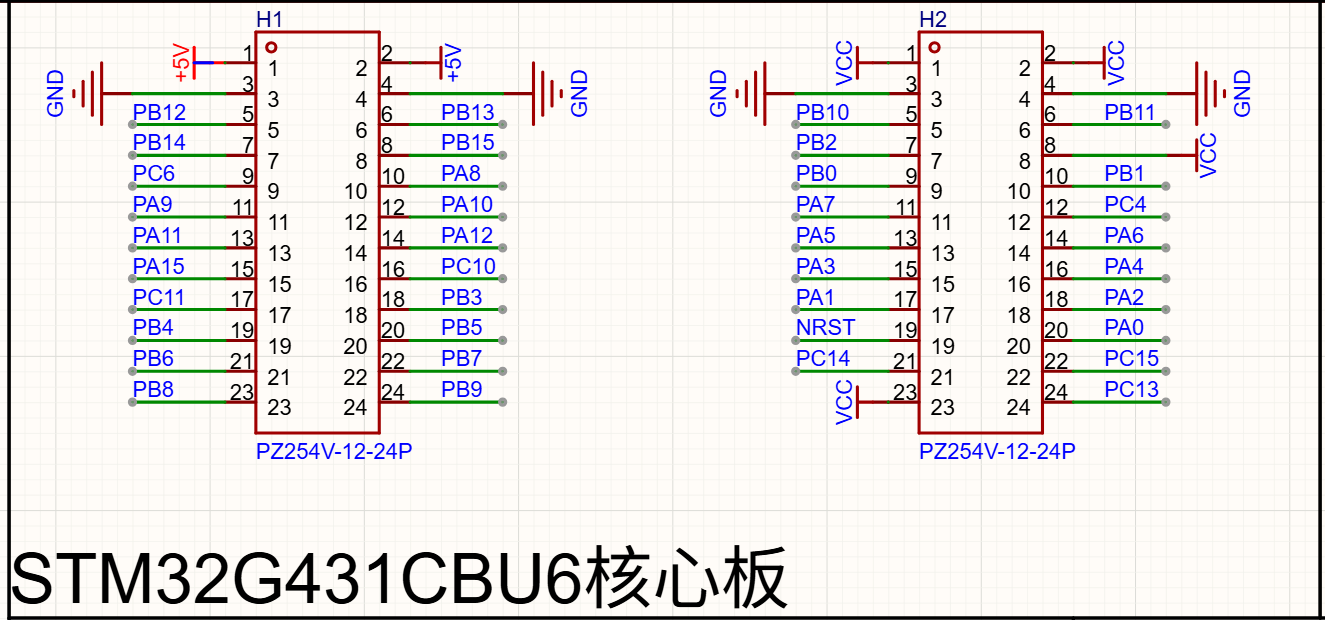
\includegraphics[width=0.5\textwidth]
    {图片/核心板电路.png}
    \caption{核心板电路}
    \label{fig:核心板电路}
\end{figure}

对于电流传感器，采用测流电阻+比例放大电路实现。为了节约电阻，选择两相低端检测的方案。即检测A，B两相的电流，C相电流通过基尔霍夫电流定律
通过$i_C=-i_A-i_B$来计算。考虑到被控设备为云台电机，标称额定电流不到1A，因此选择5mΩ作为电流检测电阻，比例放大电路放大系数配置为100。
此外，由于三相电路电流会出现负值，因此需要在比例放大电路中施加偏置。为了与MCU的ADC外设配合，选择偏置电压为ADC最大采集电压的一半，
即1.65V（通过电阻分压实现）。最终可得电流检测部分电路如下图\ref{fig:电流检测电路}所示，此时输出电压和单相电流之间的函数关系为：
\(U_o=1.65-0.5I\)
\begin{figure}[H]
    \centering
    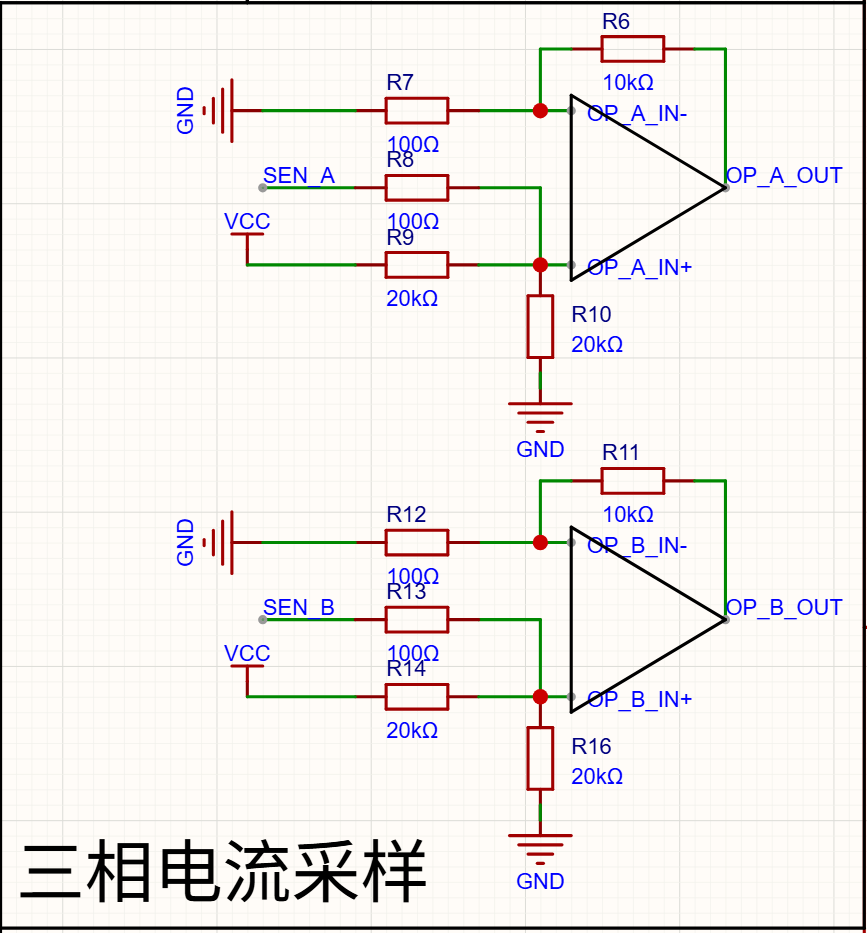
\includegraphics[width=0.5\textwidth]
    {图片/电流检测电路.png}
    \caption{电流检测电路}
    \label{fig:电流检测电路}
\end{figure}

转子位置传感器，也就是编码器，是区别于经典有感FOC和无感FOC的关键。此处选择为绝对式磁编码器，型号TLE5012BE1000。该型号传感为英飞凌公司
推出的高性能磁编码器，提供15位的绝对式角度检测分辨率，并且可以通过SSC通信协议（SPI兼容）实现与MCU的通信，驱动较为简单。为了给芯片提供
稳定的供电，选择将5V电压通过LDO降压到3.3V进行供电，通过LDO的高PSRR（电源抑制比）来确保编码器的稳定运行，并且也要通过LDO避免其他用电
电路对编码器的干扰。编码器相关电路如下图\ref{fig:编码器相关电路}所示。
\begin{figure}[H]
    \centering
    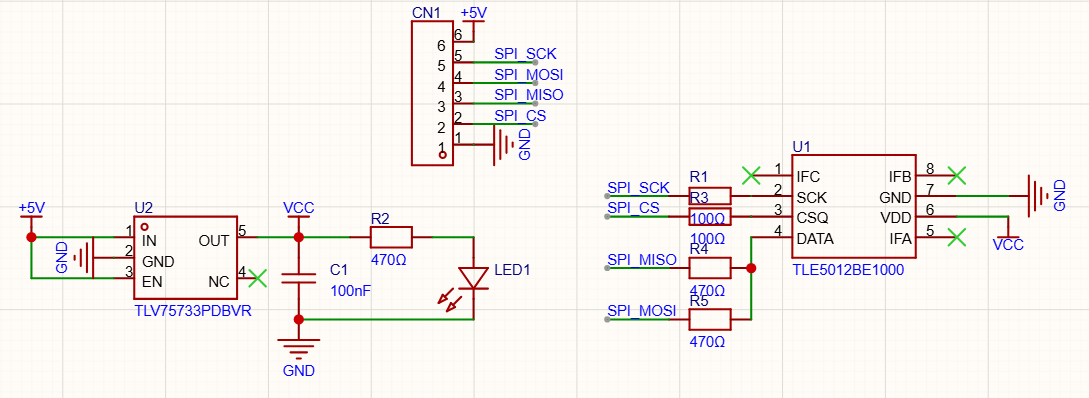
\includegraphics[width=0.5\textwidth]
    {图片/编码器相关电路.png}
    \caption{编码器相关电路}
    \label{fig:编码器相关电路}
\end{figure}

三相全桥驱动器和三相全桥电路是将PWM信号进行放大、直接实现对电机驱动的电路，其电路图与\ref{fig:三相全桥逆变电路}所示。
大部分方案选择将驱动器与电路本身分离，目的是通过用单独的功率器件构成三相全桥，提高带电机负载的能力。但是云台电机驱动电流小，
PCB设计空间有限，因此选择将驱动器与电路本身集成在一起，采用德州仪器的DRV8313作为一体式驱动器。DRV8313基于电荷泵原理实现对上桥的驱动
并且预留了每一相对应的接地端，便于通过测流电阻实现相电流检测。其单相瞬时最大电流可达2.5A，持续最大电流有效值可达1.75A，工作电压从8V到60V
，基本满足驱动云台电机的需要。相关电路图如下图\ref{fig:电机驱动电路}所示。
\begin{figure}[H]
    \centering
    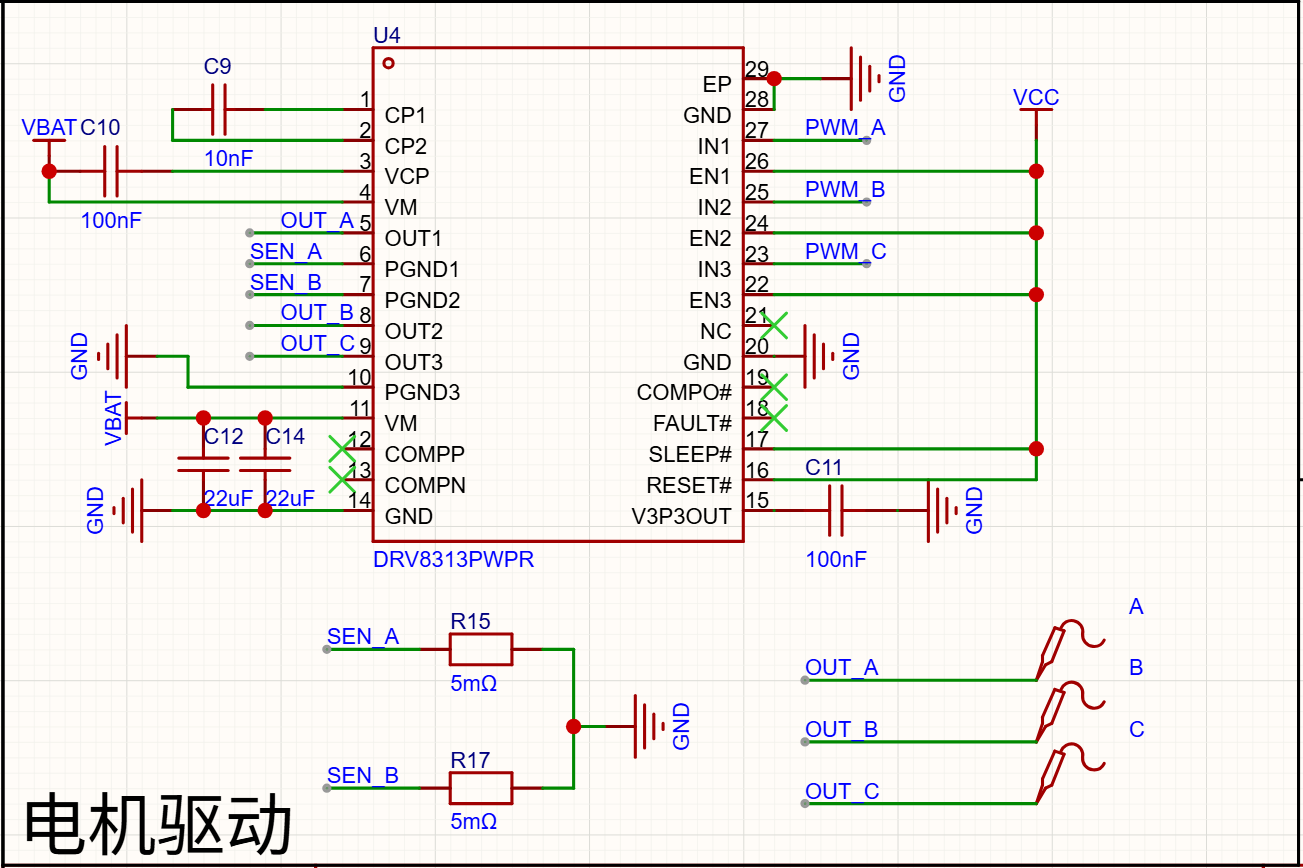
\includegraphics[width=0.5\textwidth]
    {图片/电机驱动电路.png}
    \caption{电机驱动电路}
    \label{fig:电机驱动电路}
\end{figure}

电源电路主要为各个电路提供各自需要的工作电压。对于主控MCU，需要3.3V工作电压；对于磁编码器，需要5V工作电压（之后再有编码器部分电路降压到
3.3V）；对于电机驱动电路，则是电池电压12V~24V。此外，为了确保安全，需要在电源输入端加入自恢复保险丝。
为了适应相关电压需求，采用典型的DC-DC大压差降压+LDO小压差降压方案，用DC-DC保证能量转换率，用LDO保证电压稳定性。

DC-DC采用德州仪器的LMR5140YYCR同步降压芯片，封装小（SOT-23-6）；开关频率高（1.1MHz），能够减小后续电感和电容的选型；最大输出电流2A，
足以满足控制逻辑电路供电需要；最大输入电压36V，能够匹配电机供电需要。

LDO采用德州仪器的TLV75733PDBVR，封装小（SOT-23-5），PSRR高（52dB@1MHz），能够提供稳定的3.3V电压。
电源电路相关电路如下图\ref{fig:电源电路}所示。
\begin{figure}[H]
    \centering
    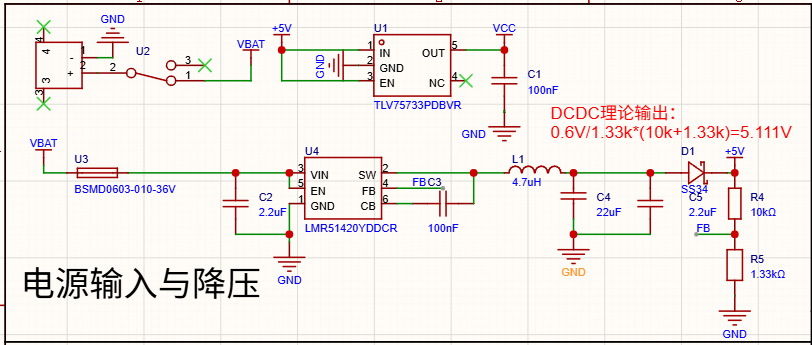
\includegraphics[width=0.5\textwidth]
    {图片/电源电路.png}
    \caption{电源电路}
    \label{fig:电源电路}
\end{figure}

其他设备包括电源指示灯、串口（向上位机发送数据）、母线电压采集电路（用于监控供电电压）等。值得一提的是母线电压检测电路。根据SVPWM计算公式
\eqref{eq:SVPWM占空比表达式}可以发现，计算三相占空比依赖母线电压$U_{dc}$。对于云台电机，工作电压范围为12V到24V，母线电压差距较大。为了
确保三相占空比计算正确，通过母线电压检测电路，让MCU通过ADC检测母线电压用于计算是很重要的。而供电一侧往往通过电池或可调直流电源实现，
电压波动较小，其主要信息集中在低频段，因此通过低通滤波电路滤除高频干扰，避免因为采集噪声导致三相占空比计算出错。
母线电压检测电路如下图\ref{fig:母线电压检测电路}所示。通过$R_4,R_5$实现$\cfrac{1.33k\Omega}{10k\Omega+1.33k\Omega}=0.1173$
的分压采集。在ADC最大输入电压3.3V情况下允许供电电压为$3.3V\div0.1173=28.13V$，足以覆盖电机供电电压。
通过$R_{7},C_6$构成RC低通滤波电路，上限截止频率为$\cfrac{1}{2\pi\times20k\Omega\times22uF}=0.36Hz$。
\begin{figure}[H]
    \centering
    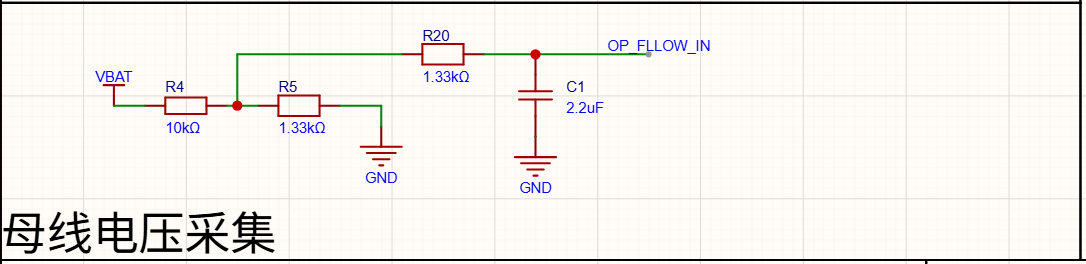
\includegraphics[width=0.5\textwidth]
    {图片/母线电压检测电路.png}
    \caption{母线电压检测电路}
    \label{fig:母线电压检测电路}
\end{figure}

\subsection{MCU外设配置与底层驱动程序}

MCU的外设配置主要关注ADC、TIM、SPI、UART等外设的配置，而底层驱动程序主要是磁编码器TLE5012B的驱动和上位机通信
撰写。两者同属底层驱动，因此在一节中讲述。使
用CLion+STM32CubeMX进行开发，因此外设配置主要在STM32CubeMX中进行图形化配置。

为了获取最高的程序运行速率，使能HSE和LSE，达到170MHz的主频。

为了实现电流检测电路中的比例放大，使能OPAMP1和OPAMP2两个模拟运算放大器外设，配置为独立模式，通过外部电阻网络构成带有直流偏置的比例放大电路。
然后将OPAMP1和OPAMP2外设的输出端连接到ADC外设，分别为ADC1$\_$IN3通道和ADC2$\_$IN3通道，将放大后的电压通过ADC采集实现电流检测。

为了实现母线电压检测，可以将母线电压检测电路的输出端连接到OPAMP3外设，并且将OPAMP3外设配置为跟随器模式，进一步提升输入阻抗，避免输入电流
带来的压降影响对母线电压的判断。同样地，将OPAMP3外设输出端连接到ADC外设，为ADC1$\_$IN12通道。

在电流环控制中，一般是每一个PWM周期都进行一次电流环控制。如果采用中断软件触发ADC采集会浪费很多时间，迫使PWM频率降低以适应计算需要的
长时间周期。因此较为简单的方法是采用硬件触发。针对ADC1和ADC2，使能注入组采集，触发源选择为TIM1的捕获比较事件4（Timer 1 Capture Compare
4 Event）。也就是说，每当TIM4$\_$CH4产生一次捕获比较事件后就会通过硬件直接触发注入组ADC采集，避免中断带来的软件延迟。

此外，由于ADC1$\_$IN3通道和ADC2$\_$IN3负责检测电机相电流，对于精度有较高的要求。而通过电阻分压得到的1.65V偏置电压会因为分压电阻
精度问题而略有偏差，需要在程序开始时进行零位矫正。通过使能规则组通道，采用软件触发即可。

接下来是核心外设定时器的配置。采用TIM1作为产生三相PWM的核心外设，预分频器PSC设置为0，计数模式选择为中心对齐模式3（Center Aligned Mode3）,
该模式下可以实现中心对齐PWM的产生。自动重装寄存器ARR设置为5664。此时PWM频率为
$f_{PWM}=\cfrac{170MHz}{2(0+1)(5664+1)}\approx 15.004kHz$，对应的电流环控制周期为66.647us。
使能TIM1$\_$CH1、TIM1$\_$CH2和TIM1$\_$CH3为PWM生成模式，用于产生三相PWM；
使能TIM1$\_$CH4为PWM生成无输出模式，将捕获比较寄存器CCR配置为ARR-1，用于产生捕获比较事件和捕获比较中断以开始电流环控制。

采用TIM2作为速度环控制中断的定时器，预分频器PSC设置为0，计数模式为向上计数，自动重装寄存器ARR设置为170000-1，此时更新中断频率为
$f_{INT}=\cfrac{170MHz}{(0+1)(170000-1+1)}= 1kHz$，对应的速度环控制周期为1ms。

通信接口在开发阶段主要使用SPI和UART。SPI通信用于和磁编码器TLE5012B进行通信，UART通信用于向上位机发送数据。根据TLE5012B数据手册，其采用
的SSC通信协议为MOSI和MISO合并为一条数据线的类SPI通信，因此将SPI外设配置为半双工主机模式（Half Duplex Master），选择软件片选；
为了尽可能减少与上位机通信占用的事件，将UART的波特率选择为2Mbps，采用奇校验，并使能DMA通道。

最后，由于FOC相关变换公式\eqref{eq:帕克变换}\eqref{eq:帕克逆变换}含有三角函数计算，采用\texttt{math.h}中的相关函数计算占用时间长，因此
一般选择查表+线性插值或硬件计算实现。STM32G431CBU6可以导入外部DSP库，也有CORDIC外设，两者都能大幅降低计算三角函数需要的事件。经过
测试发现，CORDIC外设计算三角函数时间略长于DSP库，因此采用DSP库实现三角函数计算。
\begin{figure}[H]
    \centering
    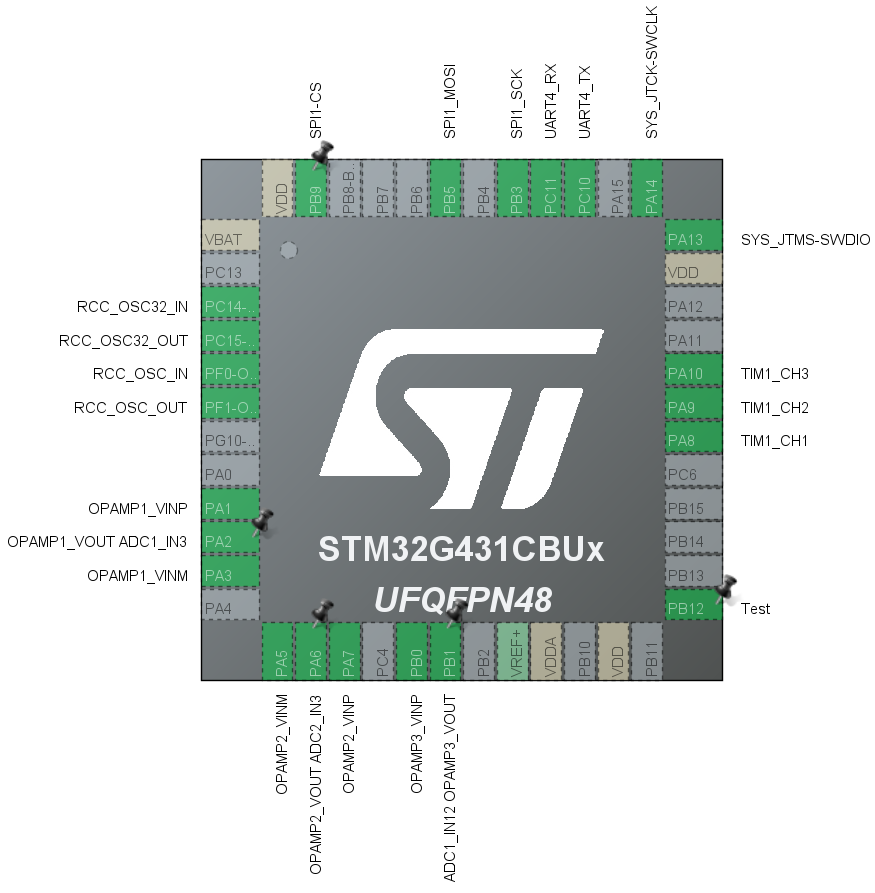
\includegraphics[width=0.5\textwidth]
    {图片/外设配置图.png}
    \caption{外设配置图}
    \label{fig:外设配置图}
\end{figure}

以上就是STM32G431CBU6的外设配置，结果如上图\ref{fig:外设配置图}所示。接下来进入底层驱动部分的撰写。

首先是对磁编码器TLE5012B的驱动文件撰写。定义头文件\texttt{MY$\_$TLE5012B.h}，包含指令码宏定义、片选信号产生与解除宏函数定义
和驱动函数声明：

\begin{lstlisting}
    #ifndef FOC_MY_TLE5012B_H
    #define FOC_MY_TLE5012B_H

    #include "main.h"

    //命令字
    #define CMD_READ_ANGLE_VALUE		0x8021  //读角度寄存器
    #define CMD_READ_SPEED_VALUE		0x8031  //读角速度寄存器
    #define CMD_READ_MOD2     0x8081  // 读配置寄存器 MOD2
    #define CMD_READ_MOD3     0x8091  // 读配置寄存器 MOD3
    #define CMD_WRITE_MOD2    0x0081  // 写配置寄存器 MOD2
    #define CMD_WRITE_MOD3    0x0091  // 写配置寄存器 MOD3

    //产生或取消片选信号宏函数定义
    #define SPI_CS_ENABLE HAL_GPIO_WritePin(SPI1_CS_GPIO_Port, SPI1_CS_Pin, GPIO_PIN_RESET);
    #define SPI_CS_DISABLE HAL_GPIO_WritePin(SPI1_CS_GPIO_Port, SPI1_CS_Pin, GPIO_PIN_SET);

    //读数据
    uint16_t TLE5012B_SPI_Read(uint16_t Order_Word);

    //写数据
    uint16_t TLE5012B_SPI_Write(uint16_t Order_Word, uint16_t WriteData);

    //读角度值
    double TLE5012B_Angle(void);

    //读角速度值
    double TLE5012B_Speed(void);

    #endif //FOC_MY_TLE5012B_H
\end{lstlisting}

定义源文件\texttt{MY$\_$TLE5012B.c}，主要是编写驱动程序的具体函数实现：

\begin{lstlisting}
    #include "MY_TLE5012B.h"

uint16_t TLE5012B_SPI_Read(uint16_t Order_Word) {
    uint16_t ReceiveData = 0;
    SPI_CS_ENABLE;
    HAL_SPI_Transmit(&hspi1, (uint8_t *) &Order_Word, 1,HAL_MAX_DELAY);
    HAL_SPI_Receive(&hspi1, (uint8_t *) &ReceiveData, 1,HAL_MAX_DELAY);
    ReceiveData = ReceiveData & 0x7FFF; //舍弃最高位状态位
    SPI_CS_DISABLE;
    return ReceiveData;
}

uint16_t TLE5012B_SPI_Write(uint16_t Order_Word, uint16_t WriteData) {
    SPI_CS_ENABLE;
    uint16_t Data[2] = {Order_Word, WriteData};
    HAL_SPI_Transmit(&hspi1, (uint8_t *) Data, 2, HAL_MAX_DELAY);
    HAL_Delay(1);
    SPI_CS_DISABLE;
    HAL_Delay(10);
}

double TLE5012B_Angle(void) {
    uint16_t Data = TLE5012B_SPI_Read(CMD_READ_ANGLE_VALUE);
    double Angle = Data * 360.0 / 32768;
    return Angle;
}

double TLE5012B_Speed(void) {
    uint16_t raw_data = TLE5012B_SPI_Read(CMD_READ_SPEED_VALUE);
    int16_t speed_counts = 0;
    if (raw_data & 0x4000) {
        //符号位为1，负数
        speed_counts = (int16_t) (raw_data | 0x8000);
    } else {
        //符号位为0，正数
        speed_counts = (int16_t) raw_data;
    }

    float delta_angle = (speed_counts / 32768.0) * 360.0;
    float omega_rad_s = delta_angle / 42.7e-6;
    return (double)omega_rad_s;
}

\end{lstlisting}

在函数\texttt{uint16$\_$t TLE5012B$\_$SPI$\_$Read(uint16$\_$t Order$\_$Word)}中，采用阻塞式SPI发送和接收函数，主要是因为在
半双工模式下需要手动切换目前SPI的状态是发送还是接收，不便于使用DMA。此外\texttt{double TLE5012B$\_$Speed(void)}函数
仅作为驱动测试，实际控制中由于读取一次数据花费时间较长，对于速度的计算一般通过角度之差实现。

另外需要编写与上位机通信相关的函数。为了减少通信占用的事件，加快通信频率，选择每一次速度环控制周期进行一次数据上传。
通信协议采用JUSTFLOAT协议，只传递\texttt{float}类型的数据。定义头文件\texttt{MY$\_$JUSTFLOAT.h}和源文件\texttt{MY$\_$JUSTFLOAT.c}
如下所示。

\begin{lstlisting}
    #ifndef FOC_MY_JUSTFLOAT_H
    #define FOC_MY_JUSTFLOAT_H

    #include "main.h"

    //JustFloat协议帧尾
    #define JUSTFLOAT_FRAME_TAIL 0x7F800000u
    //最大变量数
    #define JUSTFLOAT_MAX_VAR 16

    //串口句柄指针
    static UART_HandleTypeDef *jf_huart = NULL;

    //变量列表和变量数
    static float *jf_var_list[JUSTFLOAT_MAX_VAR];
    static uint8_t jf_var_cnt = 0;

    //实际发送数据：变量+帧尾
    static uint32_t jf_tx_buf[JUSTFLOAT_MAX_VAR + 1];

    //初始化JustFloat函数
    void JUSTFLOAT_Init(void);

    //绑定串口
    void JUSTFLOAT_BindUart(UART_HandleTypeDef *huart);

    //添加新变量
    void JUSTFLOAT_AddData(float *Data);

    //发送变量列表
    void JUSTFLOAT_SendData(void);

    #endif
\end{lstlisting}

\begin{lstlisting}
    #include "MY_JUSTFLOAT.h"

    void JUSTFLOAT_Init(void) {
        jf_var_cnt = 0;
        for (int i=0;i<JUSTFLOAT_MAX_VAR;i++) {
            jf_var_list[i] = NULL;
        }
    }

    void JUSTFLOAT_BindUart(UART_HandleTypeDef *huart) {
        jf_huart = huart;
    }

    void JUSTFLOAT_AddData(float *Data) {
        if (jf_var_cnt < JUSTFLOAT_MAX_VAR){
            jf_var_list[jf_var_cnt] = Data;
        }
        jf_var_cnt++;
    }

    void JUSTFLOAT_SendData(void) {
        uint8_t i;
        for (i = 0; i < jf_var_cnt; i++)
        {
            jf_tx_buf[i] = *(uint32_t *)jf_var_list[i];
        }
        jf_tx_buf[jf_var_cnt] = JUSTFLOAT_FRAME_TAIL;
        HAL_UART_Transmit_DMA(jf_huart,(uint8_t *)jf_tx_buf,(jf_var_cnt + 1) * sizeof(uint32_t));
    }
\end{lstlisting}

\subsection{程序初始化}

程序初始化过程是指从上电开始到进入主控制中断的过程，主要包括变量声明、外设启动、传感器零位标定三个步骤。

声明全局变量如下：

\begin{lstlisting}
//ADC采样原始数据
uint32_t ADC_Data[3] = {0, 0, 0};
//ADC采样转换后电流数据
float Current_abc[3] = {0, 0, 0};
//机械角度
float theta_m = 0;
float theta_m_last = 0;
//电角度
float theta_e = 0;
float Sin_theta_e = 0;
float Cos_theta_e = 0;
//机械角速度
float n_m = 0;
//速度环低通滤波
float n_m_last = 0;
//零位偏置
float ADC1_ZERO = 0;
float ADC2_ZERO = 0;
float Angel_ZERO = 0;
//两相静止坐标系电流
float I_alpha = 0;
float I_beta = 0;
//同步旋转坐标系电流
float I_d = 0;
float I_q = 0;
//SVPWM得到的三相占空比
float Duty_A = 0;
float Duty_B = 0;
float Duty_C = 0;
//母线电压
float Udc = U_DC_Default;
//SVPWM最大电压
float U_svpwm_max = U_DC_Default / SQRT3;
//DQ轴驱动电压
float U_d = 0;
float U_q = 0;
//电流-速度环PID控制器
Discrete_PID_Struct D_PID, Q_PID, Speed_PID;
//指令接收全局变量
uint8_t UART_Buffer[100];
float Order = 0;
uint16_t UART_Length = 0;
//电流环运行标志位
bool Current_Control_Flag = false;
\end{lstlisting}

并且宏定义可调参数如下：

\begin{lstlisting}
//数学常数
#define SQRT3 1.7320508065

//电机极对数
#define MOTOR_POLE_PAIRS 14

//速度环一阶低通滤波系数
#define Speed_Filter 0.1

//D轴电流环连续域PID参数
#define D_Kp 30
#define D_Ki 10000
#define D_Kd 0
#define D_N 10000

//Q轴电流环连续域PID参数
#define Q_Kp 30
#define Q_Ki 10000
#define Q_Kd 0
#define Q_N 10000

//速度环连续域PID参数
#define Speed_Kp 0.001
#define Speed_Ki 0.005
#define Speed_Kd 0
#define Speed_N 100

//速度环和电流环采样周期，单位s
#define Ts_Current ((__HAL_TIM_GET_AUTORELOAD(&htim1)+1)/170000000.0) * 2
#define Ts_Speed    ((__HAL_TIM_GET_AUTORELOAD(&htim2)+1)/170000000.0)

//默认母线电压，单位V
#define U_DC_Default 12

//默认给定电流，单位A
#define ID_Target_Default 0
#define IQ_Target_Default 0
//默认给定转速，单位rpm
#define Speed_Target_Default 0

//速度环输出限幅（电流环给定限幅）
#define Speed_Output_Limit 0.5

//速度环给定限幅
#define Speed_Target_Limit 350
\end{lstlisting}

完成变量声明后进行外设启动和传感器校准，两者一般分模块同时进行。

首先使能模拟运算放大器OPAMP1、OPAMP2和OPAMP3、使能ADC1和ADC2的规则组。此时TIM1和TIM2没有使能，不输出PWM，因此此时三相电流
均为零，直接采集OPAMP1和OPAMP2的输出电压，应该就是空载时的直流偏置电压。通过ADC1和ADC2的规则组阻塞式采样10次取均值，即可实现
直流偏置电压的采集。最后使能ADC1和ADC2的注入组并开启中断。代码段如下所示。

\begin{lstlisting}
    //使能模拟运算放大器
    HAL_OPAMP_Start(&hopamp1);
    HAL_OPAMP_Start(&hopamp2);
    HAL_OPAMP_Start(&hopamp3);

    //开启两个ADC校验
    HAL_ADCEx_Calibration_Start(&hadc1, ADC_SINGLE_ENDED);
    HAL_ADCEx_Calibration_Start(&hadc2, ADC_SINGLE_ENDED);
    for (int i = 0; i < 10; i++) {
        //ADC零位检测
        HAL_ADCEx_Calibration_Start(&hadc1, ADC_SINGLE_ENDED);
        HAL_ADCEx_Calibration_Start(&hadc2, ADC_SINGLE_ENDED);
        HAL_ADC_Start(&hadc1);
        if (HAL_ADC_PollForConversion(&hadc1, HAL_MAX_DELAY) == HAL_OK) {
            ADC1_ZERO += HAL_ADC_GetValue(&hadc1) / 4096.0 * 3.3;
        }
        HAL_ADC_Start(&hadc2);
        if (HAL_ADC_PollForConversion(&hadc2, HAL_MAX_DELAY) == HAL_OK) {
            ADC2_ZERO += HAL_ADC_GetValue(&hadc2) / 4096.0 * 3.3;
        }
    }
    ADC1_ZERO = ADC1_ZERO / 10.0;
    ADC2_ZERO = ADC2_ZERO / 10.0;
    //使能ADC注入组转换
    HAL_ADCEx_InjectedStart_IT(&hadc1);
    HAL_ADCEx_InjectedStart_IT(&hadc2);
\end{lstlisting}

然后进行编码器零位校准。这一部分主要是为了校准通过磁编码器读取计算出来的电角度。
考虑实际同步旋转坐标系如下图\ref{fig:控制坐标系和实际坐标系}
黑色部分所示，紫色部分是控制器所在的坐标系（控制坐标系），两者存在电角度偏差$\Delta \theta$满足
$\theta_{real}=\theta_{control}+\Delta\theta$
。设$U_d,U_q$表示实际坐标系的驱动电压，
而$U_{d_c},U_{q_c}$表示控制坐标系下的驱动电压。
\begin{figure}[H]
    \centering
    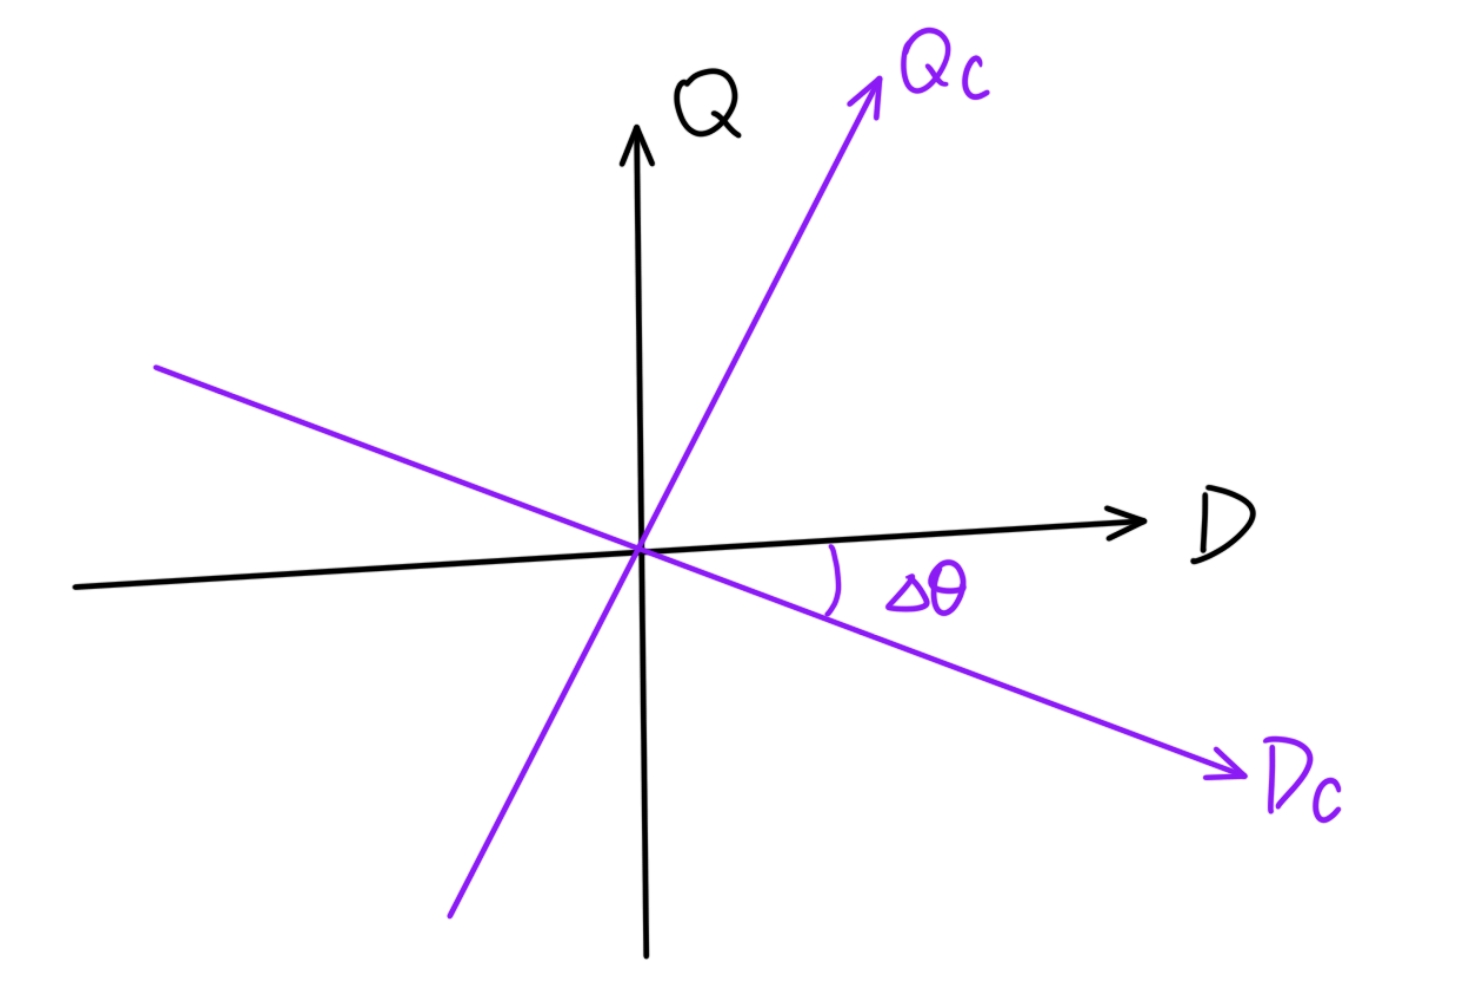
\includegraphics[width=0.3\textwidth]
    {图片/控制坐标系和实际坐标系.jpg}
    \caption{控制坐标系和实际坐标系}
    \label{fig:控制坐标系和实际坐标系}
\end{figure}

根据电磁转矩表达式\eqref{eq:同步坐标系下电磁转矩表达式（一般形式）}，可以发现$T_e\propto i_q$。而根据电路方程
\eqref{eq:同步坐标系下电路方程}可知，在初始无角速度情况下，只有通过给定$U_q$，才能使电机产生电磁转矩，使得电机旋转。
若只给定$U_d$，则电机不会旋转。根据图\ref{fig:控制坐标系和实际坐标系}可知，在给定$U_{d_c}$的情况下，编码器零位校准正确
的判别方法就是电机不发生旋转。
因此最简单的方法就是从零开始，按照特定步长递增，尝试每一个可能的$\Delta\theta$，直到电机在给定$U_d$持续一定时间
后角度增量小到可接受程度。这种方法需要长时间校准。为了解决这个问题，可以采用粗校准+细校准两部分来进行。

粗校准主要目的是缩小偏差的范围。
将编码器零位的可取范围用单位圆表示，特殊角0°、90°、180°、270°将其分为四个象限。以第一象限为例推导粗校准过程，如下图所示。
\begin{figure}[H]
    \centering
    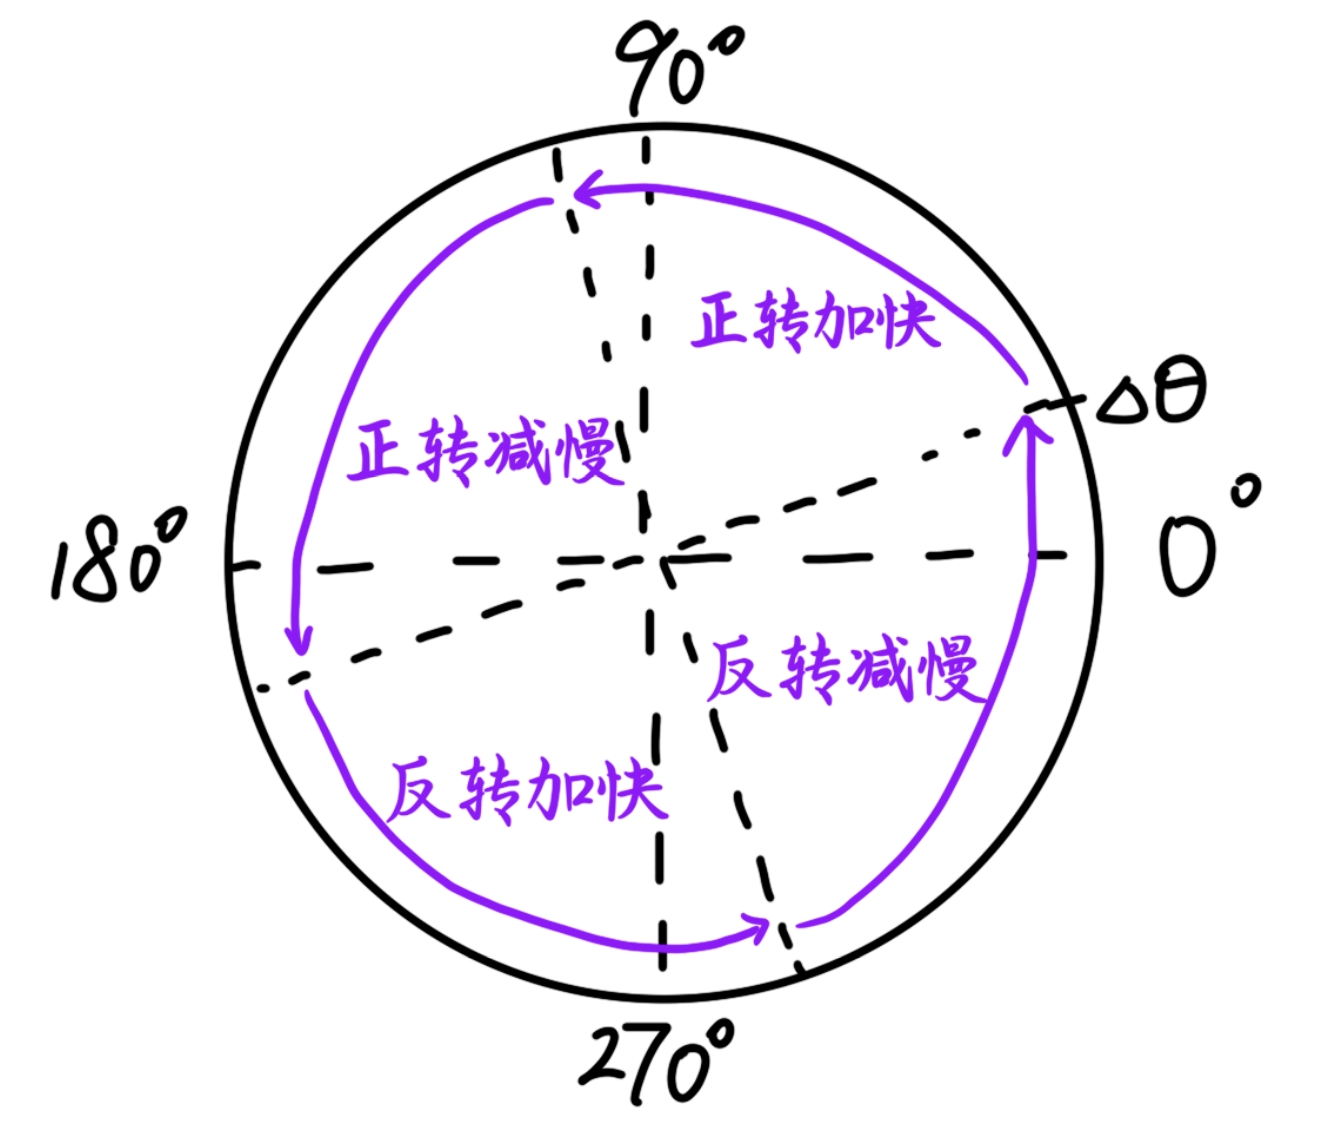
\includegraphics[width=0.3\textwidth]
    {图片/粗校准过程.jpg}
    \caption{粗校准过程}
    \label{fig:粗校准过程}
\end{figure}

假设当$U_q>0$时产生的电磁转矩在空载情况下使电机旋转的方向为正向。那么从0°开始不断增大尝试的电角度偏差，会经历反转减慢、正转加快、正转减慢
反转加快四个步骤。由于$\Delta\theta$位于第一象限，因此在0°和90°下测试得到的转速方向是不一致的（异号）。而在90°下测试得到的转速是正转的。
不难想到，通过判断0°和90°转速方向是否一致，可以判断$\Delta\theta$位于第一、第三象限还是位于第二、第四象限。而判断90°下测试得到的转速方向
就可以进一步确定$\Delta\theta$的象限，也就确定了基准值。
值得注意的是，0°和90°测试不具有唯一性，理论上只要是两个相差90°的特殊角都可以。最终得到象限判断表如下表\ref{tab:粗校准表}所示。
\begin{table}[H]
    \centering
    \begin{tabular}{|c|c|c|}
        \hline
        &90°测试点正转&90°测试点反转\\
        \hline
        90°和0°测试点转速方向相异&第一象限（0°基准）&第三象限（180°基准）\\
        \hline
        90°和0°测试点转速方向相同&第四象限（270°基准）&第二象限（90°基准）\\
        \hline
    \end{tabular}
    \caption{粗校准表}
    \label{tab:粗校准表}
\end{table}

接下来进行细校准过程。可以在粗校准基准值基础上通过特定步长自增来不断尝试$\Delta\theta$，但这同样需要较长时间。
可以从另一个角度分析，不妨假设这一过程为闭环控制：期望角速度为0，根据反馈得到的角速度偏差（$-\omega_m$），
执行特定控制律输出尝试的编码器零位，直到给定$U_d$运行一段时间电机角度基本不发生变化。

为了方便起见，假设控制器为I控制器，即下一步尝试的编码器零位满足$\Delta\theta_{next}=\Delta\theta_{current}-K_i\omega_m$。
加上校准步骤前使能TIM1和三相PWM，校准后使能电流环和速度环控制中断通道，最终得到的编码器零位校准程序如下所示。

\begin{lstlisting}
    //使能定时器
    HAL_TIM_Base_Start(&htim1);
    //三相PWM输出
    HAL_TIM_PWM_Start(&htim1, TIM_CHANNEL_1);
    HAL_TIM_PWM_Start(&htim1, TIM_CHANNEL_2);
    HAL_TIM_PWM_Start(&htim1, TIM_CHANNEL_3);
    //编码器零位校准
    int k = 0;
    Ud = 12;
    Uq = 0;
    // 基于I闭环控制模型抽象的编码器零位矫正
    int k = 0;
    U_d = U_svpwm_max;
    U_q = 0;
    float wm_0_90[2] = {0};
    for (int i = 0; i < 2; i++)
    {
      //读取起始机械角度
      theta_m_last = TLE5012B_Angle();
      // 给定Ud情况下转动
      for (int j = 0; j < 50; j++)
      {
        theta_e = TLE5012B_Angle();
        theta_e = theta_e * MOTOR_POLE_PAIRS + i * 90;
        DSP_Float_Calc_SinCos(theta_e, &Sin_theta_e, &Cos_theta_e);
        SVPWM_Calculation(&U_d, &U_q, Sin_theta_e, Cos_theta_e,U_svpwm_max, Udc, 
          &Duty_A, &Duty_B, &Duty_C);
        Set_CCR(Duty_A, Duty_B, Duty_C);
      }
      // 读取结束机械角度
      theta_m = TLE5012B_Angle();
      wm_0_90[i] = theta_m - theta_m_last;
      U_d = U_svpwm_max;
    }
    if (wm_0_90[0] * wm_0_90[1] < 0)
    {
      //零位位于第一、第三象限
      if (wm_0_90[1] < 0)
      {
        //零位位于第三象限
        Angel_ZERO = 180;
      }
      else if (wm_0_90[1] > 0)
      {
        //零位位于第一象限
        Angel_ZERO = 0;
      }
    }
    else if (wm_0_90[0] * wm_0_90[1] > 0)
    {
      //零位位于第二、第四象限
      if (wm_0_90[1] < 0)
      {
        //零位位于第二象限
        Angel_ZERO = 90;
      }
      else if (wm_0_90[1] > 0)
      {
        //零位位于第四象限
        Angel_ZERO = 270;
      }
    }
    while (k < 3)
    {
      float Angle_ZERO_Init = Angel_ZERO;
      theta_m_last = TLE5012B_Angle();
      for (int i = 0; i < 100; i++)
      {
        theta_e = TLE5012B_Angle();
        theta_e = theta_e * MOTOR_POLE_PAIRS + Angel_ZERO;
        DSP_Float_Calc_SinCos(theta_e, &Sin_theta_e, &Cos_theta_e);
        SVPWM_Calculation(&U_d, &U_q, Sin_theta_e, Cos_theta_e,U_svpwm_max, Udc, 
          &Duty_A, &Duty_B, &Duty_C);
        Set_CCR(Duty_A, Duty_B, Duty_C);
      }
      theta_m = TLE5012B_Angle();
      n_m = (1 - Speed_Filter) * (theta_m - theta_m_last) + Speed_Filter * n_m;
      U_d = U_svpwm_max;
      if (n_m < 0.5 && n_m > -0.5)
      {
        k++;
      }
      else
      {
        k = 0;
        Angel_ZERO += 0.1 * n_m;
      }
    }
\end{lstlisting}

经过测试，在选取合适的参数情况下，上述编码器零位校准方法能够较快的完成校准，但是重复性较差，且I控制参数和阈值选取不正确会导致
电机长时间卡死在校准中，无法正常进入工作状态。
此外该方法本质仍是试验方法，只不过使用I控制器的抽象和粗校准+细校准的分段方式加快的试验确定零位的速度。

另一种工业上常用的校准方法为定点测量。在A-B-C三相自然坐标系中，若给定A相电压，BC相电压很小，则磁链会被吸引到与A方向重合，此时应为
电角度的0°。为了避免单次校准误差，可以轮流给定A-B-C相电压，对应的理论电角度为0°、120°和240°。通过多次测量取平均，可以快速实现对
编码器零位的校准。校准程序如下。
\begin{lstlisting}
    int k = 0;
    U_d = U_svpwm_max;
    while(k<10)
    {
      //A相
      Set_CCR(0.9,0.1,0.1);
      HAL_Delay(500);
      theta_e = TLE5012B_Angle() * MOTOR_POLE_PAIRS;
      theta_e = fmod(theta_e, 360);
      theta_e<0?theta_e+=360:theta_e;
      Angel_ZERO += 360 - theta_e;
      //B相
      Set_CCR(0.1,0.9,0.1);
      HAL_Delay(500);
      theta_e = TLE5012B_Angle() * MOTOR_POLE_PAIRS - 120;
      theta_e = fmod(theta_e, 360);
      theta_e<0?theta_e+=360:theta_e;
      Angel_ZERO += 360 - theta_e;  
      //C相
      Set_CCR(0.1,0.1,0.9);
      HAL_Delay(500);
      theta_e = TLE5012B_Angle() * MOTOR_POLE_PAIRS + 120;
      theta_e = fmod(theta_e, 360);
      theta_e<0?theta_e+=360:theta_e;
      Angel_ZERO += 360 - theta_e;
      //计算零位
      Angel_ZERO = Angel_ZERO / 3;
      //验证
      theta_m_last = TLE5012B_Angle();
      for (int i = 0; i < 100; i++)
      {
        theta_e = TLE5012B_Angle();
        theta_e = theta_e * MOTOR_POLE_PAIRS + Angel_ZERO;
        DSP_Float_Calc_SinCos(theta_e, &Sin_theta_e, &Cos_theta_e);
        SVPWM_Calculation(&U_d, &U_q, Sin_theta_e, Cos_theta_e, U_svpwm_max, Udc, &Duty_A, &Duty_B, &Duty_C);
        Set_CCR(Duty_A, Duty_B, Duty_C);
      }
      theta_m = TLE5012B_Angle();
      n_m = (1 - Speed_Filter) * (theta_m - theta_m_last) + Speed_Filter * n_m;
      U_d = 0;
      if (n_m < 0.5 && n_m > -0.5)
      {
        break; 
      }
      else {
        k++;
        Angel_ZERO = 0;
      }
    }
\end{lstlisting}

最后一步为JUSTFLOAT相关通信协议注册变量并绑定串口，程序如下所示。

\begin{lstlisting}
    //初始化
    JUSTFLOAT_Init();
    //绑定串口
    JUSTFLOAT_BindUart(&huart4);
    //注册变量表
    JUSTFLOAT_AddData(&theta_m);
    JUSTFLOAT_AddData(&theta_e);
    JUSTFLOAT_AddData(&n_m);
    JUSTFLOAT_AddData(&Udc);
    JUSTFLOAT_AddData(&I_d);
    JUSTFLOAT_AddData(&I_q);
    // JUSTFLOAT_AddData(&Duty_A);
    // JUSTFLOAT_AddData(&Duty_B);
    // JUSTFLOAT_AddData(&Duty_C);
    JUSTFLOAT_AddData(&Angel_ZERO);
    JUSTFLOAT_AddData(&U_d);
    JUSTFLOAT_AddData(&U_q);
    JUSTFLOAT_AddData(&D_PID.Setvalue);
    JUSTFLOAT_AddData(&Q_PID.Setvalue);
    JUSTFLOAT_AddData(&Speed_PID.Setvalue);
    JUSTFLOAT_AddData(&Current_abc[0]);
    JUSTFLOAT_AddData(&Current_abc[1]);
    JUSTFLOAT_AddData(&Current_abc[2]);
\end{lstlisting}

\subsection{电流内环PI闭环控制}

电流内环PI控制由TIM1$\_$CH4的比较捕获事件/中断触发，主要包含数据采集、克拉克-帕克变换求取$I_d,I_q$、DQ轴PID控制运算、SVPWM调制、设定
三相占空比几个步骤。

数据采集包括对转子位置的采集和对三相电流的采集。由于三相电流采集通过比较捕获事件触发，触发速度远超中断，因此选择在比较捕获中断中通过与
磁编码器TLE5012B的通信获取转子位置。而由于通信需要的时间较长，因此在比较捕获中断过程中会被ADC注入组转换完成中断打断。但是由于ADC1和ADC2都
会采集数据、都会触发注入组转换完成中断。为了避免重复计算，考虑到ADC1需要对两个通道（一个A相电流，一个母线电压）转换而ADC2只需要对
一个通道转换，即ADC1总是比ADC2慢转换完成，因此可以只在ADC1转换完成后进行数据处理（还原电流、进行电流低通滤波、计算C相电流）。
又由于ADC注入组转换完成中断优先级较高，会比比较捕获中断更先执行完，因此将后续控制函数入口放在比较捕获中断末尾。数据采集流程图和程序段
如下所示。
\begin{figure}[H]
    \centering
    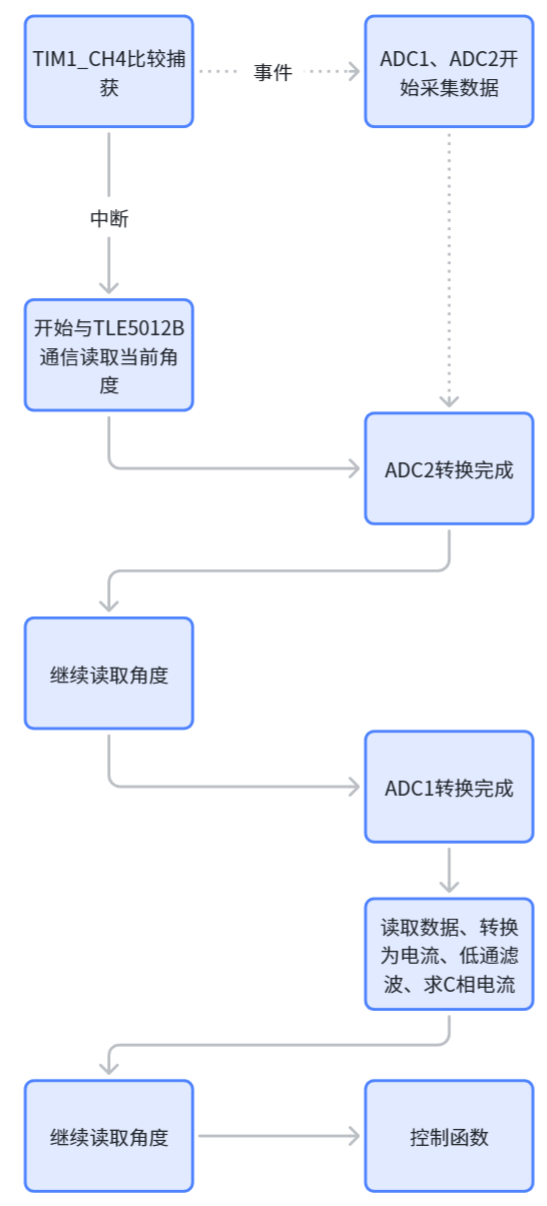
\includegraphics[width=0.2\textwidth]
    {图片/数据采集流程图.png}
    \caption{数据采集流程图}
    \label{fig:数据采集流程图}
\end{figure}

\begin{lstlisting}
    void HAL_ADCEx_InjectedConvCpltCallback(ADC_HandleTypeDef *hadc) {
    //ADC原始采样值
    extern uint32_t ADC_Data[3];
    //ADC转换后三相电流值
    extern float Current_abc[3];
    //ADC零位偏置
    extern float ADC1_ZERO;
    extern float ADC2_ZERO;
    //野值剔除暂存变量
    float Current_last[3];
    extern Discrete_PID_Struct Q_PID;
    //由于ADC1需要采集两个数据（其中有一个电压数据），ADC2只需要采集一个数据，因此ADC1总会比ADC2更晚进入中断
    if (hadc == &hadc1) {
        HAL_GPIO_WritePin(Test_GPIO_Port,Test_Pin, GPIO_PIN_SET);
        // ADC_Data[0] = HAL_ADCEx_InjectedGetValue(&hadc1, ADC_INJECTED_RANK_1);
        // ADC_Data[1] = HAL_ADCEx_InjectedGetValue(&hadc2, ADC_INJECTED_RANK_1);
        // ADC_Data[2] = HAL_ADCEx_InjectedGetValue(&hadc1, ADC_INJECTED_RANK_2);
        ADC_Data[0] = hadc1.Instance->JDR1;
        ADC_Data[1] = hadc2.Instance->JDR1;
        ADC_Data[2] = hadc1.Instance->JDR2;
        //野值剔除
        Current_last[0] = Current_abc[0];
        Current_last[1] = Current_abc[1];
        Current_last[2] = Current_abc[2];
        Current_abc[0] = -((ADC_Data[0] / 4096.0) * 3.3 - ADC1_ZERO) * 2;
        Current_abc[1] = -((ADC_Data[1] / 4096.0) * 3.3 - ADC2_ZERO) * 2;
        Current_abc[2] = -Current_abc[0] - Current_abc[1];
        if((Current_abc[0] > 0.45) || (Current_abc[0] < -0.45))
        {
            Current_abc[0] = Current_last[0];
            Current_abc[1] = Current_last[1];
            Current_abc[2] = Current_last[2];
        }
        else if((Current_abc[1] > 0.45) || (Current_abc[1] < -0.45))
        {
            Current_abc[0] = Current_last[0];
            Current_abc[1] = Current_last[1];
            Current_abc[2] = Current_last[2];
        }
        else if((Current_abc[2] > 0.45) || (Current_abc[2] < -0.45))
        {
            Current_abc[0] = Current_last[0];
            Current_abc[1] = Current_last[1];
            Current_abc[2] = Current_last[2];
        }
    }

    void HAL_TIM_PWM_PulseFinishedCallback(TIM_HandleTypeDef *htim) {
    if ((htim->Instance == TIM1) && (htim->Channel == HAL_TIM_ACTIVE_CHANNEL_4)) {
        //电流环运行标志位
        extern bool Current_Control_Flag;
        extern float theta;
        theta = TLE5012B_Angle();
        //如果电流环未运行，才进行电流环
        if (Current_Control_Flag == false)
        {
            Current_Control();
        }
    }
}
}
\end{lstlisting}

在控制函数中，主要执行计算电角度、进行克拉克-帕克变换求取当前的$I_d,I_q$、进行PID控制计算、SVPWM调制、设定三相占空比几个步骤。

克拉克-帕克变换需要相关的函数计算都已经用DSP库实现，只需要调用即可，相关函数如下所示。

\begin{lstlisting}
    void Clarke_Trans(float A, float B, float C, float *alpha, float *beta) {
        arm_clarke_f32(A, B, alpha, beta);
    }

   void Inv_Clarke_Trans(float alpha, float beta, float *A, float *B, float *C) {
        arm_inv_clarke_f32(alpha, beta, A, B);
        *C = 0 - *A - *B;   
    }

    void Park_Trans(float alpha, float beta, float Sin, float Cos, float *D, float *Q) {
        arm_park_f32(alpha, beta, D, Q, Sin, Cos);
    }

    void Inv_Park_Trans(float D, float Q, float Sin, float Cos, float *alpha, float *beta) {
        arm_inv_park_f32(D, Q, alpha, beta, Sin, Cos);
    }
\end{lstlisting}

采用PID控制器。在连续域中的传递函数为$G_{PID}(s)=K_p+\cfrac{K_i}{s}+K_d\cfrac{s}{\frac 1N s+1}$，采用双线性变换
$s=\cfrac{2}{T_s}\cfrac{1-z^{-1}}{1+z^{-1}}$，接下来推导采用双线性变换后的离散域传递函数与差分方程表示。

对于比例项保持不变为$K_p$，积分项双线性变换后为$\cfrac{K_iT_s}{2}\times\cfrac{1+z^{-1}}{1-z^{-1}}$

微分项的双线性变换后为$K_d\times\cfrac{2}{T_s}\cfrac{1-z^{-1}}{1+z^{-1}}\times\cfrac{1}{\frac{1}{N}\times
\frac{2}{T_s}\frac{1-z^{-1}}{1+z^{-1}}+1}$，
展开得到$\cfrac{2K_d}{T_s}\times\cfrac{NT_s(1-z^{-1})}{2(1-z^{-1})+NT_s(1+z^{-1})}$，化简可得
$\cfrac{2K_dN}{NT_s+2}\times\cfrac{1-z^{-1}}{1+\frac{NT_s-2}{NT_s+2}z^{-1}}$。

定义离散域下的系数$P=K_p,I=\cfrac{K_iT_s}{2},D=\cfrac{2K_dN}{NT_s+2},N_d=\cfrac{NT_s-2}{NT_s+2}$，则总的传递函数可以表示为
\begin{align*}
    G(z)&=P+I\cfrac{1+z^{-1}}{1-z^{-1}}+D\cfrac{1-z^{-1}}{1+N_dz^{-1}}\\
    & = \cfrac{P(1-z^{-1})(1+N_dz^{-1})+
    I(1+z^{-1})(1+N_dz^{-1})+
    D(1-z^{-1})^2}{(1-z^{-1})(1+N_dz^{-1})}\\
    & =\cfrac{(P+I+D)+(PN_d-P+IN_d+I-2D)z^{-1}+(D+IN_d-PN_d)z^{-2}}{1+(N_d-1)z^{-1}-N_dz^{-2}}\\
    & = \cfrac{Y(z)}{E(z)}
\end{align*}

由在控制系统中习惯采用增量式实现，增量式的传递函数为\(G'(z)=(1-z^{-1})G(z)\)，因此可得：
\begin{align*}
    G'(z)&=(1-z^{-1})G(z)\\
    & = \cfrac{(P+I+D)+(PN_d-2P+IN_d-3D)z^{-1}+(3D-2PN_d+P-I)z^{-2}+(PN_d-D-IN_d)z^{-3}}{1+(N_d-1)z^{-1}-N_dz^{-2}}\\
    & = \cfrac{b_0+b_1z^{-1}+b_2z^{-2}+b_3z^{-3}}{1+a_1z^{-1}+a_2z^{-2}}\\
    & = \cfrac{\Delta Y(z)}{E(z)}
\end{align*}

因此PID控制器结构体、初始化函数和执行的函数如下所示。

\begin{lstlisting}
    //PID控制器结构体
    typedef struct {
        float a1, a2;
        float b0, b1, b2, b3;
        float Error_Record[3];
        float Output_Delta_Record[2];
        float Error_Now;
        float Output_Delta_Now;
        float Setvalue;
    } Discrete_PID_Struct;

    //PID控制器结构体初始化函数
    void PID_Struct_Init(float Kp, float Ki, float Kd, float N, float Ts, float Default_Set, Discrete_PID_Struct* PID)
    {
        float P = Kp;
        float I = Ki * Ts / 2.0;
        float D = (2 * Kd * N) / (N * Ts + 2.0);
        float Nd = (N * Ts - 2.0) / (N * Ts + 2.0);
        if(Kd == 0)
        {
            Nd = 0;
            D = 0;
        }
        //增量式实现：输入误差，输出控制增量
        PID->Error_Record[0] = 0;
        PID->Error_Record[1] = 0;
        PID->Error_Record[2] = 0;
        PID->Output_Delta_Record[0] = 0;
        PID->Output_Delta_Record[1] = 0;
        PID->Error_Now = 0;
        PID->Output_Delta_Now = 0;
        PID->Setvalue = Default_Set;

        PID->a1 = -(Nd-1);
        PID->a2 = -(-Nd);
        PID->b0 = P + I + D;
        PID->b1 = P*Nd-2*P+I*Nd-3*D;
        PID->b2 = 3*D-2*P*Nd+P-I;
        PID->b3 = P*Nd-D-I*Nd;
    }

    //PID控制器执行函数
    void Discrete_PID_Controller(Discrete_PID_Struct* PID)
    {   
        //增量式实现：输入误差，输出控制增量
        float Temp_Output_Delta = 0;
        Temp_Output_Delta += PID->a1 * PID->Output_Delta_Record[0];
        Temp_Output_Delta += PID->a2 * PID->Output_Delta_Record[1];
        Temp_Output_Delta += PID->b0 * PID->Error_Now;
        Temp_Output_Delta += PID->b1 * PID->Error_Record[0];
        Temp_Output_Delta += PID->b2 * PID->Error_Record[1];
        Temp_Output_Delta += PID->b3 * PID->Error_Record[2];
        PID->Output_Delta_Now = Temp_Output_Delta;
        PID->Output_Delta_Record[1] = PID->Output_Delta_Record[0];
        PID->Output_Delta_Record[0] = PID->Output_Delta_Now;
        PID->Error_Record[2] = PID->Error_Record[1];
        PID->Error_Record[1] = PID->Error_Record[0];
        PID->Error_Record[0] = PID->Error_Now;
    }
\end{lstlisting}

SVPWM调制按照\eqref{eq:零序分量表达式}和\eqref{eq:SVPWM占空比表达式}计算即可。但根据电压极限圆表达式\eqref{eq:SVPWM电压极限圆}，
需要检查给定的$U_d,U_q$是否在电压极限圆内。如果不在电压极限圆内，需要进行线性放缩。相关函数如下所示。

\begin{lstlisting}
    void SVPWM_Calculation(float* Ud, float* Uq, float Sin, float Cos, float U_svpwm_max,float Udc,
    float* Duty_A, float* Duty_B,float* Duty_C)
    {
        float U_alpha, U_beta = 0;
        float U_ABC[3] = {0};
        float U_max, U_min = 0;
        float U_0 = 0;
        float u_mag = 0;
        if (U_svpwm_max == 0)
        {
            return;
        }
        arm_sqrt_f32((*Ud) * (*Ud) + (*Uq) * (*Uq), &u_mag);
        if (u_mag > U_svpwm_max)
        {
            u_mag = U_svpwm_max / u_mag;

        }
        else
        {
            u_mag = 1;
        }
        *Ud = (*Ud) * u_mag;
        *Uq = (*Uq) * u_mag;
        Inv_Park_Trans(*Ud, *Uq, Sin, Cos, &U_alpha, &U_beta);
        Inv_Clarke_Trans(U_alpha, U_beta, &U_ABC[0], &U_ABC[1], &U_ABC[2]);
        arm_max_f32(U_ABC, 3, &U_max, NULL);
        arm_min_f32(U_ABC, 3, &U_min, NULL);
        U_0 = -0.5 * (U_max + U_min);
        *Duty_A = 0.5 + (U_0 + U_ABC[0]) / Udc;
        *Duty_B = 0.5 + (U_0 + U_ABC[1]) / Udc;
        *Duty_C = 0.5 + (U_0 + U_ABC[2]) / Udc;
}   
\end{lstlisting}

为了增强程序的鲁棒性，避免后续在尝试更改PWM频率时需要连带修改程序，在设定三相占空比函数中通过用三相占空比乘ARR的值来确定需要给定的CCR。
相关函数如下所示。

\begin{lstlisting}
    void Set_CCR(float Duty_A, float Duty_B, float Duty_C) {
        int ARR = __HAL_TIM_GET_AUTORELOAD(&htim1);
        __HAL_TIM_SET_COMPARE(&htim1, TIM_CHANNEL_1, ARR*Duty_A);
        __HAL_TIM_SET_COMPARE(&htim1, TIM_CHANNEL_2, ARR*Duty_B);
        __HAL_TIM_SET_COMPARE(&htim1, TIM_CHANNEL_3, ARR*Duty_C);
    }   
\end{lstlisting}

最后调用上述函数的控制函数\texttt{void Current$\_$Control()}如下所示。

\begin{lstlisting}
    void Current_Control()
    {
        //机械角度
        extern float theta_m;
        extern float Angel_ZERO;
        //电角度
        extern float theta_e;
        //三相自然坐标系
        extern float Current_abc[3];
        //两相静止坐标
        extern float I_alpha;
        extern float I_beta;
        //同步旋转坐标系
        extern float I_d;
        extern float I_q;
        //三相占空比
        extern float Duty_A;
        extern float Duty_B;
        extern float Duty_C;
        //DQ轴电压
        extern float U_d;
        extern float U_q;
        //母线电压
        extern float Udc;
        //SVPWM最大电压
        extern float U_svpwm_max;
        //DQ轴电流控制器
        extern Discrete_PID_Struct D_PID;
        extern Discrete_PID_Struct Q_PID;
        //三角函数
        extern float Sin_theta_e;
        extern float Cos_theta_e;
        //电流环运行标志位
        extern bool Current_Control_Flag;
        //置位标志位
        Current_Control_Flag = true;
        //计算电角度
        theta_e = theta_m * MOTOR_POLE_PAIRS + Angel_ZERO;
        theta_e = fmod(theta_e, 360);
        theta_e<0?theta_e+=360:theta_e;
        //计算三角函数
        DSP_Float_Calc_SinCos(theta_e, &Sin_theta_e, &Cos_theta_e);
        //计算电流
        Clarke_Trans(Current_abc[0], Current_abc[1], Current_abc[2], &I_alpha, &I_beta);
        Park_Trans(I_alpha, I_beta, Sin_theta_e, Cos_theta_e, &I_d, &I_q);
        D_PID.Error_Now = D_PID.Setvalue - I_d;
        Q_PID.Error_Now = Q_PID.Setvalue - I_q;
        Discrete_PID_Controller(&D_PID);
        Discrete_PID_Controller(&Q_PID);
        U_d += D_PID.Output_Delta_Now;
        U_q += Q_PID.Output_Delta_Now;
        //SVPWM调制
        SVPWM_Calculation(&U_d, &U_q, Sin_theta_e, Cos_theta_e, U_svpwm_max, Udc, &Duty_A, &Duty_B, &Duty_C);
        // Q_PID.Output_Record[0] = U_q;
        // D_PID.Output_Record[0] = U_d;
        //设定CCR值
        Set_CCR(Duty_A, Duty_B, Duty_C);
        //重置标志位
        Current_Control_Flag = false;
        HAL_GPIO_WritePin(Test_GPIO_Port,Test_Pin, GPIO_PIN_RESET);
    }
\end{lstlisting}
由于采用了增量式的控制器实现形式，接收输入为每个控制周期中的偏差值，输出控制增量，天然具有很强的抗积分饱和特性，因此没有
使用额外的抗积分饱和手段。
通过给定$I_d$检测电流闭环控制效果。在给定$I_d=0.2A$和$I_d=-0.2A$情况下电流响应如下图所示。

\begin{figure}[H]
    \begin{minipage}{0.5\textwidth}
        \centering
        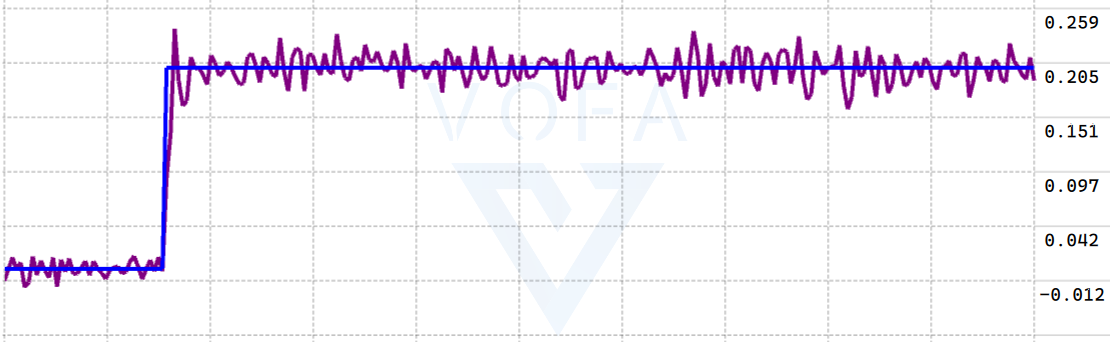
\includegraphics[width=1.1\textwidth]{图片/Id=0.2A阶跃响应图.png}
        \caption{$I_d$=0.2A阶跃响应图}
    \end{minipage}
    \begin{minipage}{0.5\textwidth}
        \centering
        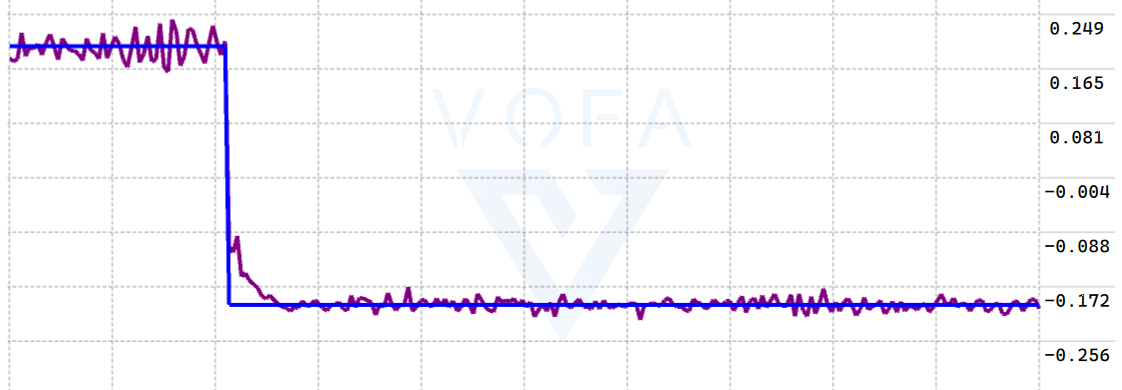
\includegraphics[width=1.1\textwidth]{图片/Id=-0.2A阶跃响应图.png}
        \caption{$I_d$=-0.2A阶跃响应图}
    \end{minipage}
\end{figure}

\subsection{速度外环PI闭环控制}

速度环的控制较之电流环基本一致，但是计算量上远不如电流环，控制周期也更长。因此选择向上位机传输数据的任务放在速度环控制周期中执行。

在TIM2的更新中断中进行数据采集，主要是求解此时的机械角速度（单位rpm），并且对母线电压采集结果转换为实际电压值，最后进入速度环控制函数。
相关函数如下所示。

\begin{lstlisting}
    void HAL_TIM_PeriodElapsedCallback(TIM_HandleTypeDef *htim) {
        extern float theta_m;
        extern float theta_m_last;
        extern float n_m;
        extern float n_m_last;
        extern float Udc;
        extern float U_svpwm_max;
        extern uint32_t ADC_Data[3];
        if (theta_m - theta_m_last < 10 && theta_m - theta_m_last > -10) {
            n_m = (theta_m - theta_m_last) / (Ts_Speed * 6);
        }
        n_m = (1-Speed_Filter) * n_m_last + Speed_Filter * n_m;
        n_m_last = n_m;
        theta_m_last = theta_m;
        Udc = ADC_Data[2] *0.00686;
        U_svpwm_max = Udc / SQRT3;
        Speed_Control();
        JUSTFLOAT_SendData();
    }
\end{lstlisting}

在速度环控制函数中，主要是执行速度环PID运算。采用$I_d=0$的控制策略，则速度环的输出就是Q轴电流环的给定值。为了避免堵转时速度环控制输出过高
导致Q轴电流环输出过高烧损电机，此处也需要对速度环控制器输出做限幅处理。相关函数如下所示。

\begin{lstlisting}
    void Speed_Control()
    {
        //DQ轴电流控制器
        extern Discrete_PID_Struct D_PID;
        extern Discrete_PID_Struct Q_PID;
        //速度环控制器
        extern Discrete_PID_Struct Speed_PID;
        //当前角速度
        extern float n_m;
        //速度环给定限幅
        if(Speed_PID.Setvalue < -Speed_Target_Limit)
        {
            Speed_PID.Setvalue = -Speed_Target_Limit;
        }
        else if(Speed_PID.Setvalue > Speed_Target_Limit)
        {
            Speed_PID.Setvalue = Speed_Target_Limit;
        }
        Speed_PID.Error_Now = Speed_PID.Setvalue - n_m;
        Discrete_PID_Controller(&Speed_PID);
        Q_PID.Setvalue += Speed_PID.Output_Delta_Now;
        //采用Id=0，Iq给定的控制策略
        if (Q_PID.Setvalue < -Speed_Output_Limit)
        {
            Q_PID.Setvalue = -Speed_Output_Limit;
        }
        else if (Q_PID.Setvalue > Speed_Output_Limit)
        {
            Q_PID.Setvalue = Speed_Output_Limit;
        }
    }
\end{lstlisting}
采用给定速度值300rpm，速度环输出限幅0.5A。无负载情况下的速度阶跃响应如下图所示（纵轴单位rpm）。
\begin{figure}[H]
    \centering
    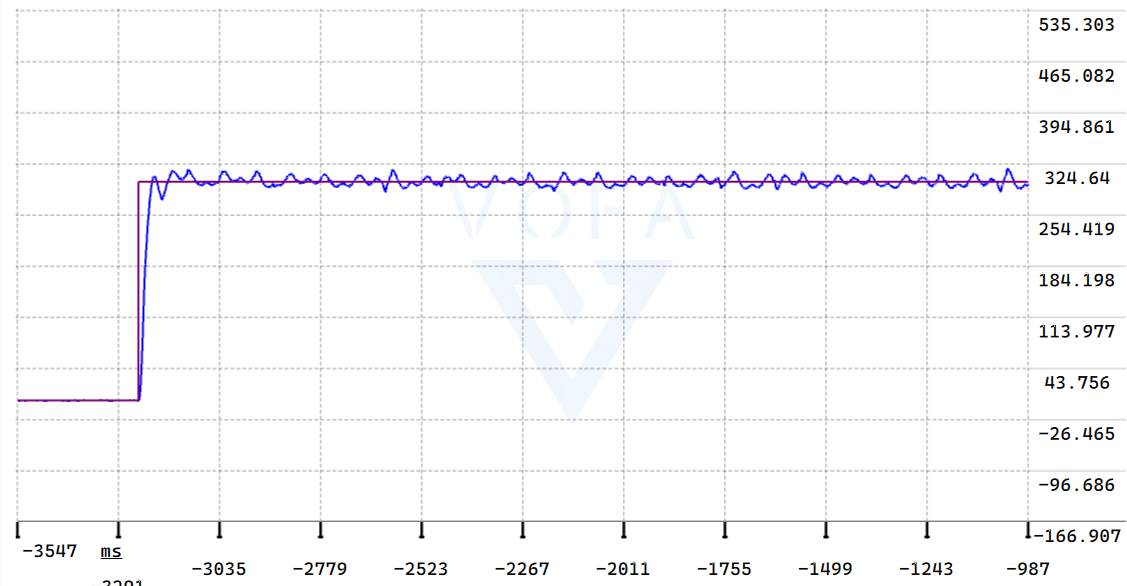
\includegraphics[width=0.6\textwidth]
    {图片/速度阶跃响应图.png}
    \caption{$n_m=300rpm$阶跃响应图}
\end{figure}

通过设置速度环输出限幅，能够确保在堵转情况下电机的安全性。在上述条件下堵转电机，DQ轴电流响应如下图所示（紫线表示
$I_d$，粉线表示$I_q$）。
\begin{figure}[H]
    \centering
    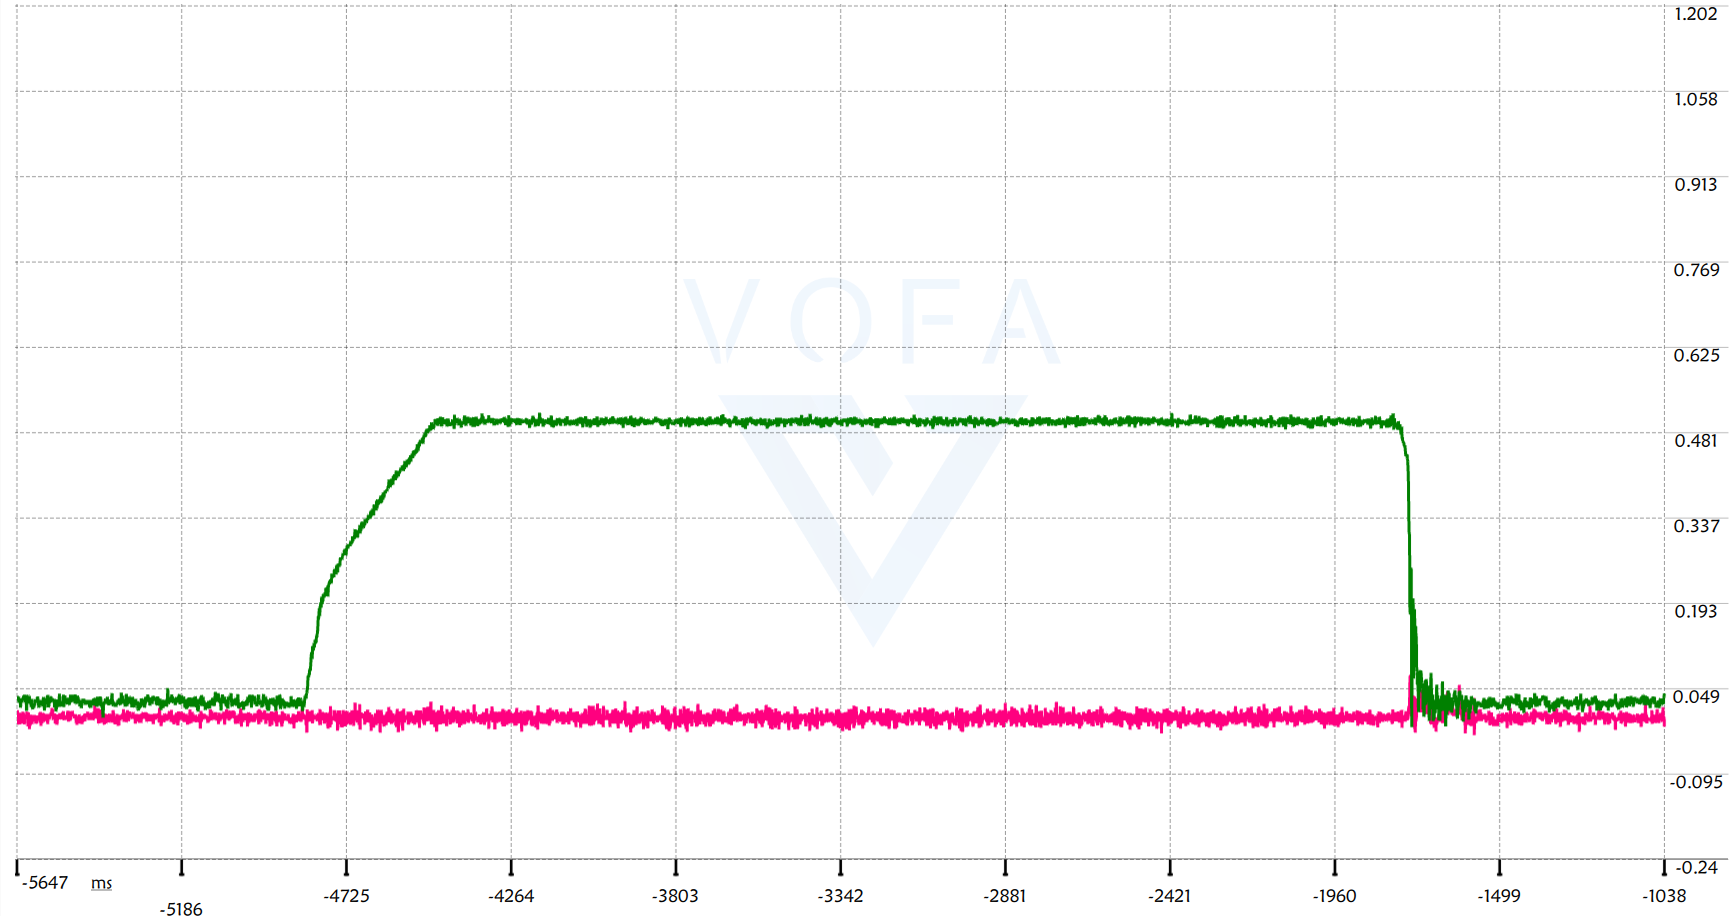
\includegraphics[width=0.6\textwidth]
    {图片/DQ电流响应图.png}
    \caption{DQ轴电流响应图}
\end{figure}

上述过程中，当堵转发生时，反电动势消失，导致DQ电流同时升高，直到控制输出电压达到SVPWM调制极限。松开时，
由于增量式控制器对饱和的天然抵抗性，能够快速的实现退饱和。

另外，为了方便调试，通过UART4的DMA接收不定长数据的功能，通过接收上位机传来的指令来调整设定值，其中断回调函数如下所示。
\begin{lstlisting}
    void HAL_UARTEx_RxEventCallback(UART_HandleTypeDef *huart, uint16_t Size) {
    extern uint8_t  UART_Buffer[100];
    extern float Order;
    extern uint16_t UART_Length;
    extern Discrete_PID_Struct D_PID,Q_PID,Speed_PID;
    UART_Length = Size;
    if (UART_Length > 0 && UART_Length < 100)
    {
        UART_Buffer[UART_Length] = '\0';
        Order = atof((const char *)UART_Buffer);
    }
    HAL_UARTEx_ReceiveToIdle_DMA(&huart4, UART_Buffer, 100);
    //以下三个选择其一进行设置
    Speed_PID.Setvalue = Order;
    // D_PID.Setvalue = Order;
    // Q_PID.Setvalue = Order;
}
\end{lstlisting}


\newpage
\section{永磁同步电机的参数辨识}

\subsection{相电阻测量}
永磁同步电机的电路方程\eqref{eq:同步坐标系下电路方程}如下：
\begin{equation}
    \begin{bmatrix}
        u_d\\u_q
    \end{bmatrix}
    =\begin{bmatrix}R_s&-\omega_eL_q\\\omega_eL_d&R_s\end{bmatrix}
    \begin{bmatrix}i_d\\i_q\end{bmatrix}
    +\begin{bmatrix}L_d&0\\0&L_q\end{bmatrix}
    \begin{bmatrix}\dot{i}_d\\\dot{i}_q\end{bmatrix}
    +\begin{bmatrix}0\\\psi_m\omega_e\end{bmatrix}
    \tag{\ref{eq:同步坐标系下电路方程}}
\end{equation}

电参数辨识，就是要对上述电路方程的中的参数进行辨识，包括相电阻\(R_s\)，D轴同步电感\(L_d\)，Q轴同步电感\(L_q\)，
以及永磁体磁链\(\psi_m\)。

首先进行相电阻的辨识。在理想情况下电机堵转，电角速度\(\omega_e=0\)，则电路方程退化为：
\begin{equation*}
    \begin{cases}
        u_d = R_si_d+L_d\cfrac{di_d}{dt}\\
        u_q = R_si_q+L_q\cfrac{di_q}{dt}
    \end{cases}
\end{equation*}

在给定\(u_d,u_q\)阶跃的情况下，稳态时电流恒定，稳态电流\(i_d=\cfrac{u_d}{R_s},i_q=\cfrac{u_q}{R_s}\)。因此可以在不同
给定\(u_d,u_q\)阶跃的情况下，通过测量稳态时\(i_d,i_q\)的值，来辨识\(R_s\)。

需要注意的是，由于稳态电流只受相电阻影响，因此只要确保电机稳态时不转动即可，中途可以因为锁轴不完全微动。

分别给定\(u_d\)和\(u_q\)，以0.1V为间隔，从-5V到5V测量稳态电流，得到曲线如下图所示。
\begin{figure}[H]
    \centering
    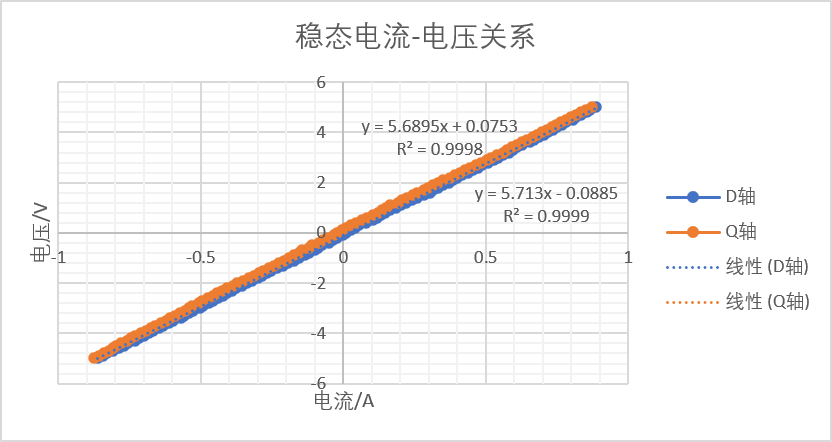
\includegraphics[width=0.6\textwidth]
    {图片/相电阻辨识曲线.png}
    \caption{相电阻辨识曲线}
\end{figure}

D轴拟合稳态电压电流关系式为\(U_d = 5.713I_d-0.0885\)，决定系数\(R_D^2=0.9999\)；
Q轴拟合稳态电压电流关系式为\(U_q = 5.6895I_q+0.0753\)，决定系数\(R_Q^2=0.9999\)。
两者平均可得相电阻辨识结果为
\begin{equation*}
    R_{sO}=5.70125\Omega
\end{equation*}

\subsection{基于相间电感测量的同步电感估测}

为了方便对后续同步电感测量结果进行判断，这里首先进行基于相间电感的同步电感估测。
对于永磁同步电机，在自然坐标系A-B-C下，每一相的自感和互感满足如下两式：

\begin{minipage}{0.5\textwidth}
    \begin{equation*}
        \begin{cases}
            L_A=L_{s0}-L_{s2}\cos2\theta_e\\
            L_B=L_{s0}-L_{s2}\cos(2\theta_e-\cfrac{4\pi}{3})\\
            L_C=L_{s0}-L_{s2}\cos(2\theta_e+\cfrac{4\pi}{3})
        \end{cases}
    \end{equation*}
\end{minipage}
\begin{minipage}{0.5\textwidth}
    \begin{equation*}
        \begin{cases}
            M_{AB}=M_{BA}=M_{s0}-M_{s2}\cos(2\theta_e+\cfrac{4\pi}{3})\\
            M_{BC}=M_{CB}=M_{s0}-M_{s2}\cos2\theta_e\\
            M_{AC}=M_{CA}=M_{s0}-M_{s2}\cos(2\theta_e-\cfrac{4\pi}{3})
        \end{cases}
    \end{equation*}
\end{minipage}

相间电感测量的具体步骤为：将一相开路，使用LCR电桥测量从另外两相看进去得到的等效电感。LCR电桥测量原理是注入恒定幅值和频率的
电压正弦波，通过稳态正弦电流响应，分析幅值和相位偏差，进而得到等效阻抗。因此测量电感可以表示为\(L=\cfrac{d\psi}{di}\)，其中
\(\psi\)表示等效磁链。

以C相开路，从AB相看进去测量相间电感为例。设此时\(i_A=i\)，则\(i_B=-i\)而\(i_C=0\)。根据磁链的定义式，可得A相磁链\(\psi_A\)和B
相磁链\(\psi_B\)的表达式为：
\begin{equation*}
    \begin{cases}
        \psi_A=L_Ai_A+M_{BA}i_B+M_{CA}i_C=(L_{s0}-L_{s2}\cos2\theta_e)i+
        (M_{s0}-M_{s2}\cos(2\theta_e+\cfrac{4\pi}{3}))(-i)\\
        \psi_B=L_Bi_B+M_{AB}i_A+M_{CB}i_C=(L_{s0}-L_{s2}\cos(2\theta_e-\cfrac{4\pi}{3}))(-i)+
        (M_{s0}-M_{s2}\cos(2\theta_e+\cfrac{4\pi}{3}))i
    \end{cases}
\end{equation*}

从AB之间看进去的等效磁链为\(\psi_{AB}=\psi_A-\psi_B\)。带入可得：
\begin{equation*}
    \psi_{AB}=2(L_{s0}-M_{s0})i
    -iL_{s2}(\cos2\theta_e+\cos(2\theta_e-\cfrac{4\pi}{3}))
    +iM_{s2}(\cos(2\theta_e+\cfrac{4\pi}{3})+\cos(2\theta_e+\cfrac{4\pi}{3}))
\end{equation*}

测量得到的电感表达式为\(L_{AB}=\cfrac{d\psi_{AB}}{di}\)，代入可得：
\begin{equation*}
    L_{AB}=2(L_{s0}-M_{s0})
    -L_{s2}(\cos2\theta_e+\cos(2\theta_e-\cfrac{4\pi}{3}))
    +M_{s2}(\cos(2\theta_e+\cfrac{4\pi}{3})+\cos(2\theta_e+\cfrac{4\pi}{3}))
\end{equation*}

化简可得：
\begin{equation*}
    L_{AB}=2(L_{s0}-M_{s0})+(L_{s2}+2M_{s2})\cos(2\theta_e-\cfrac{2\pi}{3})
\end{equation*}

结合同步电感定义式\eqref{eq:同步电感定义式}如下：
\begin{equation*}
    \begin{cases}
        L_d=L_{s0}-M_{s0}-\cfrac{L_{s2}}{2}-M_{s2}\\
        L_q=L_{s0}-M_{s0}+\cfrac{L_{s2}}{2}+M_{s2}
    \end{cases}
\end{equation*}

可得AB相间电感表达式为：
\begin{equation*}
    L_{AB}=(L_d+L_q)+(L_q-L_d)\cos(2\theta_e-\cfrac{2\pi}{3})
\end{equation*}

同理可得BC和AC相间电感表达式，结合AB相间电感表达式可得：
\begin{equation}
    \begin{cases}
        L_{AB}=(L_d+L_q)+(L_q-L_d)\cos(2\theta_e-\cfrac{2\pi}{3})
        \\
        L_{BC}=(L_d+L_q)+(L_q-L_d)\cos2\theta_e
        \\
        L_{AC}=(L_d+L_q)+(L_q-L_d)\cos(2\theta_e+\cfrac{2\pi}{3})
    \end{cases}
    \label{eq:相间电感表达式}
\end{equation}

因此可以通过测量相间电感随电角度变化的曲线幅值和平均值，来估测同步电感\(L_d=\cfrac{L_{\min}}{2}\)和\(L_q=\cfrac{L_{\max}}{2}\)。
在不同频率下测量相间电感曲线如下图所示（样本数为36）。
\begin{figure}[H]
    \begin{minipage}{0.5\textwidth}
        \centering
        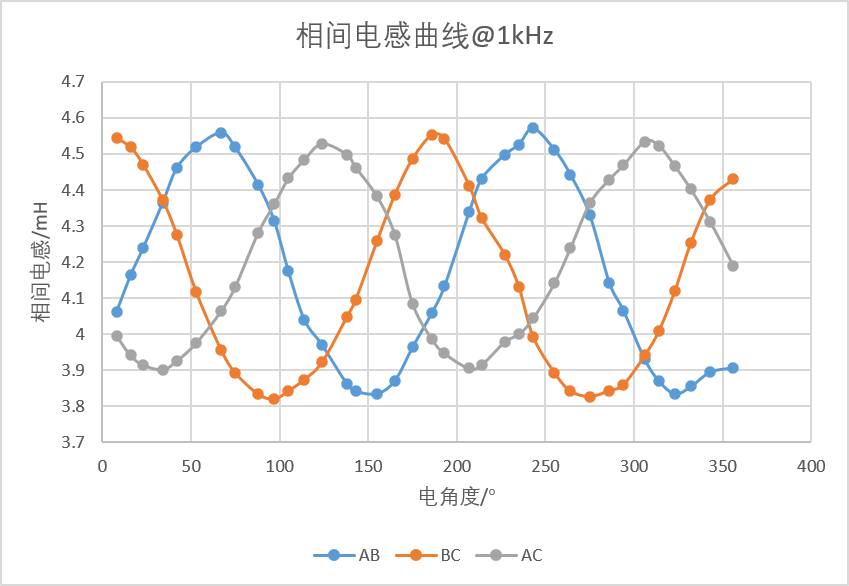
\includegraphics[width=\textwidth]{图片/1kHz相间电感测量曲线.png}
        \caption{1kHz相间电感测量曲线}
    \end{minipage}
        \begin{minipage}{0.5\textwidth}
        \centering
        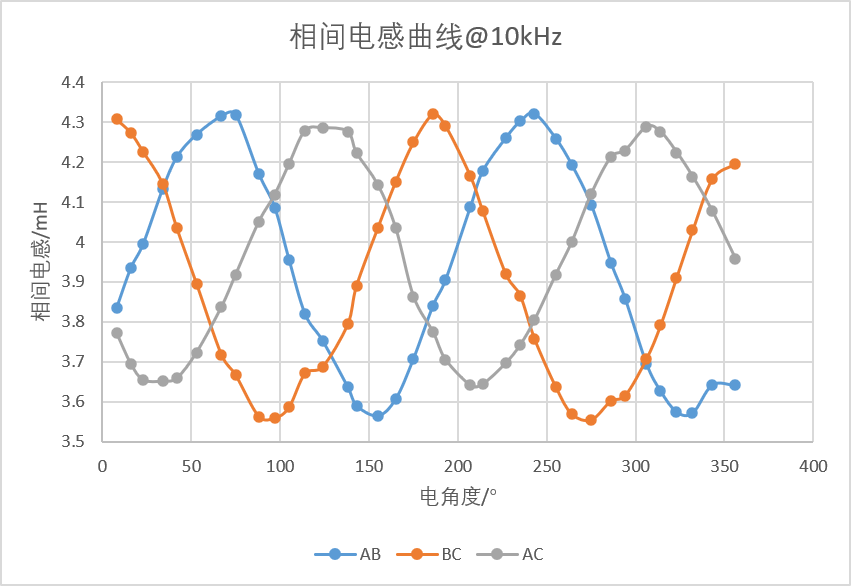
\includegraphics[width=\textwidth]{图片/10kHz相间电感测量曲线.png}
        \caption{10kHz相间电感测量曲线}
    \end{minipage}
\end{figure}

根据线性回归知识，若某输出与多个输入满足线性关系\(y=a_0+\sum\limits_{i=1}^ma_mx_m\)，则进行n次测量后
定义输出数据向量\(Y=\begin{bmatrix}y_1\\y_2\\\vdots\\y_n\end{bmatrix}_{n\times 1}\)和输入数据矩阵
\(X=\begin{bmatrix}
    1&x_{11}&x_{12}&\cdots&x_{1m}\\1&x_{21}&x_{22}&\cdots&x_{2m}\\\vdots&\vdots&\vdots&\ddots&\vdots\\1&x_{n1}&x_{n2}&\cdots&x_{nm}
\end{bmatrix}_{n\times(m+1)}\)，并且有待定系数矩阵\(A=\begin{bmatrix}a_0\\a_1\\a_2\\\vdots\\a_m\end{bmatrix}_{(m+1)\times 1}\)。那么理想情况下
满足\(Y=XA\)，而由于噪声和测量误差存在，实际上各个数据满足\(Y=XA+\varepsilon\)。

经典的最小二乘拟合方法要求将所有数据的残差平方和最小，即损失函数为\(S(A)=(Y-XA)^T(Y-XA)\)。
展开可得\(S(A)=Y^TY-Y^TXA-A^TX^TY+A^TX^TXA\)，其中根据维度分析可知\(Y^TXA=A^TX^TY\)为标量，因此
损失函数可以写为\(S(A)=Y^TY+A^TX^TXA-2A^TX^TY\)。

求解损失函数梯度为\(\cfrac{\partial S(A)}{\partial A}=2X^TXA-2X^TY\)。令其为零求解使得损失函数最小的系数矩阵表达式为：
\begin{equation}
    \hat{A}=(X^TX)^{-1}X^TY。
    \label{eq:多元线性回归公式}
\end{equation}

这也就是多元线性回归的参数计算公式。根据相间电感表达式\eqref{eq:相间电感表达式}可知，任意两相之间的测量电感可以一般地表示为
\begin{equation*}
    L=a_0+a_1\cos2\theta_e+a_2\sin2\theta_e
\end{equation*}

将\(\cos2\theta_e\)和\(\sin2\theta_e\)视为两个输入，则可以通过多元线性回归计算最小二乘拟合参数。拟合结果如下图所示。
\begin{figure}[H]
    \begin{minipage}{0.5\textwidth}
        \centering
        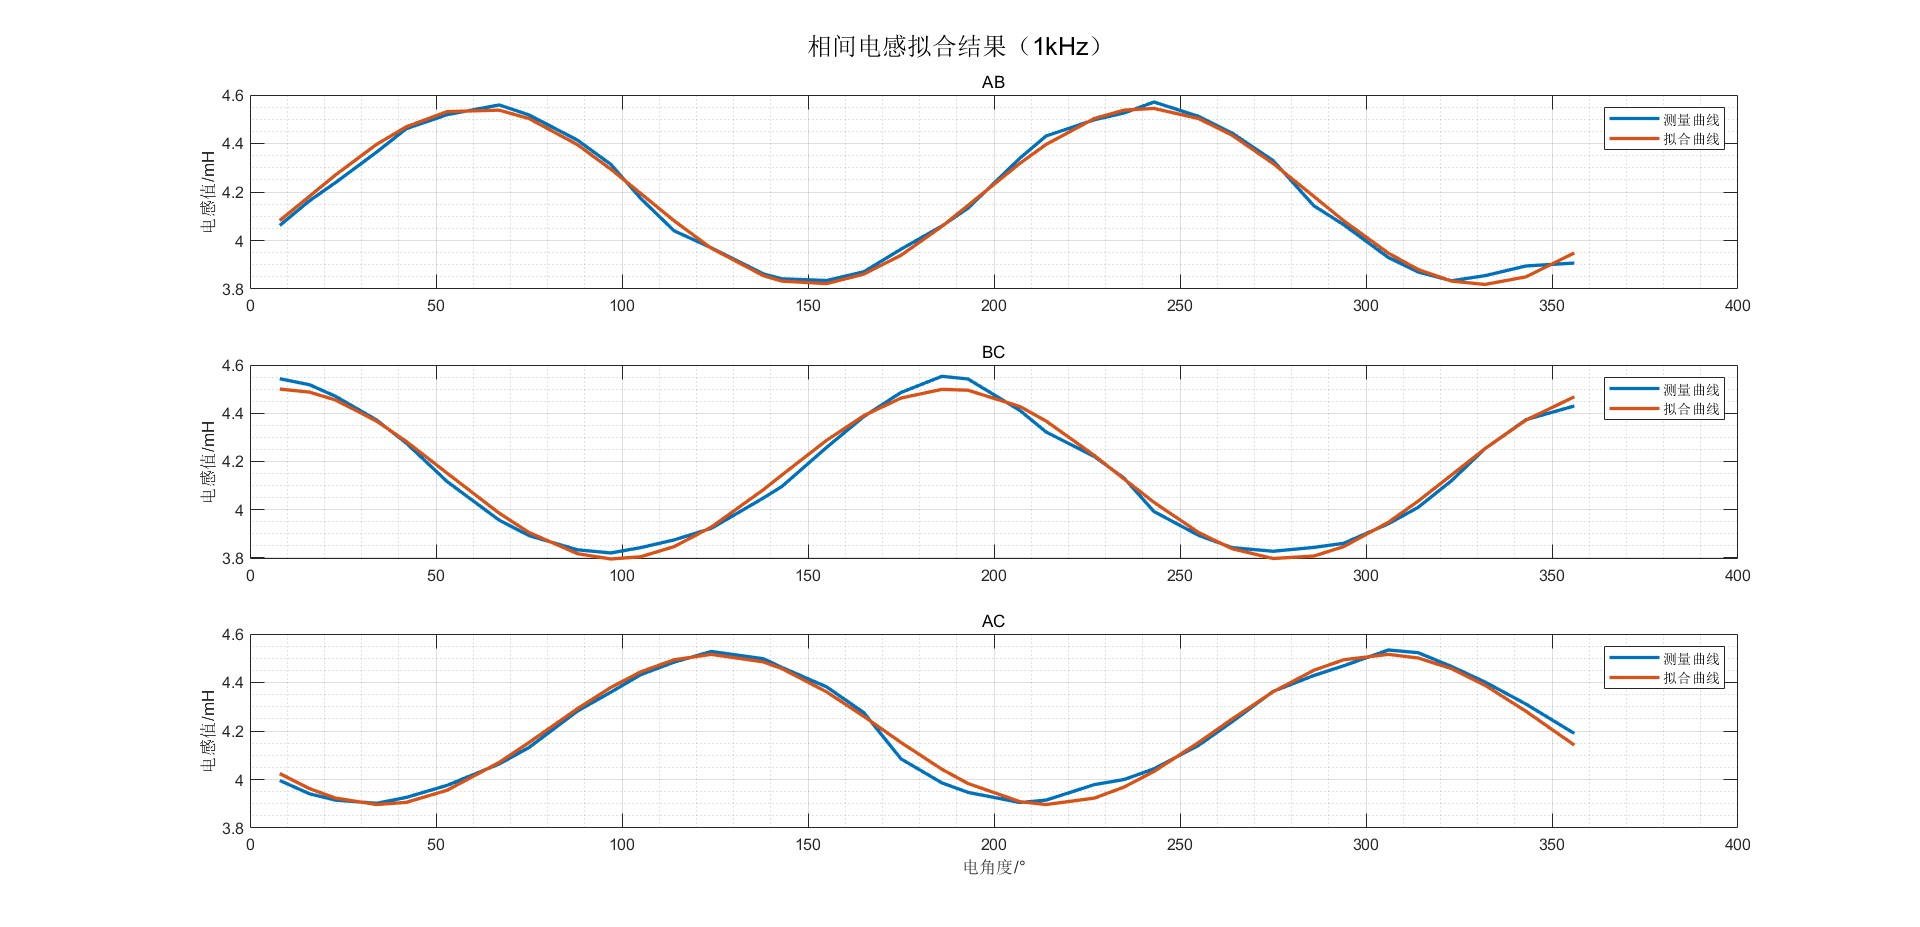
\includegraphics[width=\textwidth]{图片/1kHz相间电感拟合结果.jpg}
        \caption{1kHz相间电感拟合结果}
    \end{minipage}
        \begin{minipage}{0.5\textwidth}
        \centering
        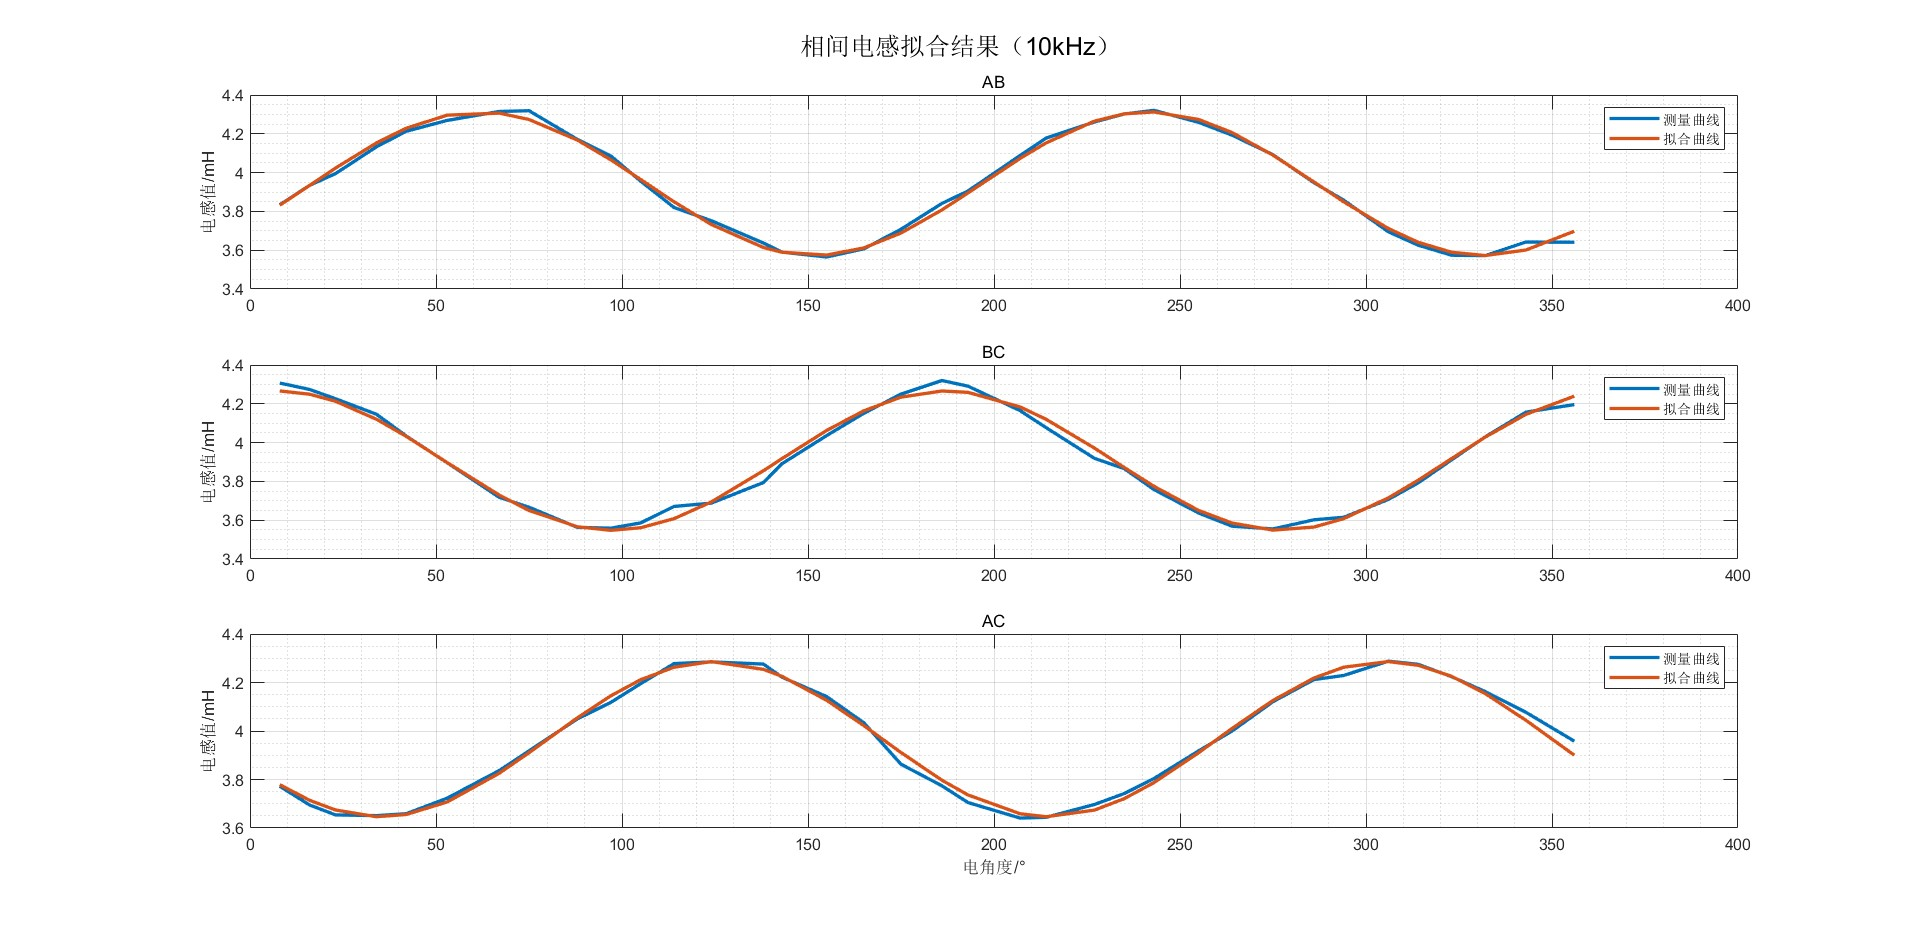
\includegraphics[width=\textwidth]{图片/10kHz相间电感拟合结果.jpg}
        \caption{10kHz相间电感拟合结果}
    \end{minipage}
\end{figure}

线性回归为：
\begin{table}[H]
    \centering
    \begin{tabular}{|c|c|c|c|}
        \hline
        测试条件&拟合结果&决定系数\(R^2\)&调整决定系数\(R^2_{adj}\)\\
        \hline
        AB@1kHz&
        \(\begin{aligned}L &= 4.1821-0.19224\cos2\theta_e+0.30851\sin2\theta_e\\
        &=4.1821+0.3635\cos(2\theta_e-121.93°)\end{aligned}\)
        &0.99242&0.99196\\
        \hline
        BC@1kHz&
        \(\begin{aligned}L &= 4.1473+0.33811\cos2\theta_e+0.10075\sin2\theta_e\\
        &=4.1473+0.3528\cos(2\theta_e-16.594°)\end{aligned}\)
        &0.98795&0.98722\\
        \hline
        AC@1kHz&
        \(\begin{aligned}L &= 4.2064-0.10595\cos2\theta_e-0.29117\sin2\theta_e\\
        &=4.2064+0.30985\cos(2\theta_e+109.99°)\end{aligned}\)
        &0.98689&0.98610\\
        \hline
        AB@10kHz&
        \(\begin{aligned}L &= 3.9427-0.20384\cos2\theta_e+0.30907\sin2\theta_e\\
        &=3.9427+0.37024\cos(2\theta_e-123.41°)\end{aligned}\)
        &0.99367&0.99329\\
        \hline
        BC@10kHz&
        \(\begin{aligned}L &= 3.9071+0.34803\cos2\theta_e+0.089177\sin2\theta_e\\
        &=3.90717+0.35927\cos(2\theta_e-14.372°)\end{aligned}\)
        &0.98844&0.98774\\
        \hline
        AC@10kHz&
        \(\begin{aligned}L &= 3.9664-0.10916\cos2\theta_e-0.3009\sin2\theta_e\\
        &=3.9664+0.32009\cos(2\theta_e+109.94°)\end{aligned}\)
        &0.99228&0.99181\\
        \hline
    \end{tabular}
    \caption{多元线性回归表}
    \label{tab:多元线性回归表}
\end{table}
根据回归结果分析，每组的决定系数\(R^2\)
\footnote{决定系数\(R^2\)定义为 \(1-\cfrac{SSE}{SST}\)，其中SSE为残差平方和\(\sum\limits_{i=1}^n(\hat{y}_i-y_i)^2\)，
SST表示总平方和\(\sum\limits_{i=1}^n(y_i-\bar{y})^2\)，分别表示“回归可解释的异变”和“总异变度”，是进行线性回归
结果评估的典型标准。}
和根据样本进行的调整决定系数\(R^2_{adj}\)
\footnote{调整决定系数定义为 \(1-\cfrac{SSE}{SST}\times\cfrac{n-1}{n-k-1}\)，其中n表示总样本量，k表示
待估计参数个数，主要是为了修正决定系数会随着待估计参数个数升高而自然升高的问题。}
均不小于0.98，线性回归的效果好。

接下来计算估计的\(L_d\)和\(L_q\)。在多元线性回归中的残差\(\varepsilon = Y - XA\)认为是服从正态分布的，即\(\varepsilon\sim N(0,\sigma^2)\)，
那么其方差的无偏估计为\(\hat{\sigma^2} = \cfrac{SSE}{n-k}\)，其中SSE表示残差的平方和，n为样本个数（此处为36），而
k为待估计参数个数（此处为3）。使用n-k而不是n是因为数据本身估计了k个参数，真正的随机信息只有n-k个维度。

根据多元线性回归公式\eqref{eq:多元线性回归公式}，将理论值\(Y=XA+\varepsilon\)代入可得：
\begin{equation*}
    \begin{aligned}
        \hat{A} &= (X^TX)^{-1}X^T(XA+\varepsilon)\\
        &=(X^TX)^{-1}X^TXA+(X^TX)^{-1}X^T\varepsilon\\
        &= A + (X^TX)^{-1}X^T\varepsilon
    \end{aligned}
\end{equation*}

由于残差服从正态分布，根据上式可知估计参数也应服从多元正态分布，数学推导可知其服从\(\hat{A}\sim N(A,\sigma^2(X^TX)^{-1})\)
，其中\(\sigma^2(X^TX)^{-1}\)为协方差矩阵。由于残差的真实方差\(\sigma^2\)未知，因此用上文计算得到的
残差方差的无偏估计\(\hat{\sigma^2} = \cfrac{SSE}{n-k}\)代替，即估计参数的协方差矩阵为
\(C = \hat{\sigma^2}X^TX^{-1}\)。根据误差的传递公式，对于某个变量\(y=f(x_1,x_2,\cdots,x_n)\)，
若已知输入变量的标准差\(\sigma_{x_i}\)和测量值\(x_i\)，则可以估计输出的测量值为
\(\hat{y}=f(x_1,\cdots,x_n)\)和标准差\(\sigma_y=\sqrt{(\nabla f)^T C (\nabla f)}\)。

针对拟合结果\(L=a_0+a_1\cos2\theta_e+a_2\sin2\theta_e\)，结合相间电感公式\eqref{eq:相间电感表达式}可以得到
\(L_d,L_q\)的计算式为：
\begin{equation*}
    \begin{cases}
        L_d =\cfrac{a_0-\sqrt{a_1^2+a_2^2}}{2}\\
        L_q =\cfrac{a_0+\sqrt{a_1^2+a_2^2}}{2}
    \end{cases}
\end{equation*}

两者的梯度为：

\begin{minipage}{0.5\textwidth}
    \begin{equation*}
        \nabla L_d =\begin{bmatrix}\cfrac{1}{2}\\-\cfrac{a_1}{2\sqrt{a_1^2+a_2^2}}\\
        -\cfrac{a_2}{2\sqrt{a_1^2+a_2^2}}\end{bmatrix}
    \end{equation*}
\end{minipage}
\begin{minipage}{0.5\textwidth}
    \begin{equation*}
        \nabla L_q =\begin{bmatrix}\cfrac{1}{2}\\
        \cfrac{a_1}{2\sqrt{a_1^2+a_2^2}}\\
        \cfrac{a_2}{2\sqrt{a_1^2+a_2^2}}\end{bmatrix}
    \end{equation*}
\end{minipage}

计算可得各组的估计\(L_d,L_q\)和标准差为：
\begin{table}[H]
    \centering
    \begin{tabular}{|c|c|c|c|c|}
        \hline
        测试条件&\(L_d\)估计值&\(L_d\)标准差&\(L_q\)估计值&\(L_q\)标准差\\
        \hline
        AB@1kHz&
        1.90928&0.00337&2.27278&0.00338\\
        \hline
        BC@1kHz&
        1.89725&0.00415&2.25006&0.00417\\
        \hline
        AC@1kHz&
        1.94828&0.00383&2.25813&0.00381\\
        \hline
        AB@10kHz&
        1.78625&0.00313&2.15649&0.00315\\
        \hline
        BC@10kHz&
        1.77392&0.00414&2.13319&0.00415\\
        \hline
        AC@10kHz&
        1.82315&0.00303&2.14324&0.00301\\
        \hline
    \end{tabular}
    \caption{估计结果和标准差}
    \label{tab:估计结果和标准差}
\end{table}

从估计值来看，在10kHz下测量的结果明显小于在1kHz下测量的结果，
这是高频信号趋肤效应
\footnote{频率较高时，电流会集中在导体的表面，而不会进入导体内部。趋肤效应会导致内磁链降低，等效电感
降低。}、铁芯涡流损耗
\footnote{交变磁通在铁芯中感应涡流，产生去磁效应，等效于在电感两端并联了随频率升高而降低的涡流电阻，
导致表观电感下降。}等效应的综合作用结果。而标准差相较于估计值的百分比不超过\(0.2\%\)，整体极小，
而发现不同相间测量组的估计值相差超过可达0.05mH，远大于标准差的0.003mH，这说明
存在无法被正态分布所解释的系统误差。

此外，相间电感测量是在单频点上进行的分析，而后续使用的Ho-Kalman辨识算法是典型的最小子空间辨识算法，
是在宽频带上进行的辨识算法，两者在参数的测量辨识原理上存在本质的不同。
\footnote{Ho-Kalman辨识是对时域Hankel矩阵的低秩逼近，最小化时域误差，用帕塞瓦尔定理可以等效为
对频域能量的加权最小二乘拟合，即寻求能够最小化频域能量残差平方和的传递函数。这其中
的权重隐含在系统响应中，响应能量越强的频段拥有更大的权重。这使得在各个频点上的权重不止依赖于输入信号，
也依赖于待测系统本身。在宽频带信号和脉动磁场作用下，涡流损耗加剧，使
得\(L_d\)和\(L_q\)相较于LCR电桥的准静止测量有较大的变化，而DQ轴磁路不同，
两者的饱和特性与动态响应天然存在差异。在上述情况下Ho-Kalman辨识算法往往与LCR测量结果
有较大差异。此外，Ho-Kalman对象不是只有电机，也包含逆变器等其他非理想因素，这些因素却恰恰是
实际控制中必须考虑的。因此LCR测量的分析结果只能作为简单的电感数量级、相对关系、凸极率分析，不可作为
实际控制设计参数。}

综上所述，选取六组的平均值±0.5倍极差作为同步电感的LCR测量估计结果：
\begin{equation*}
    \begin{cases}
        L_d\in(1.76917,1.94354)\textrm{mH}
        \\
        L_q\in(2.13252,2.27211)\textrm{mH}
    \end{cases}
\end{equation*}

\subsection{辨识算法的仿真分析}
在正式进入实际测量之前，在本小节搭建仿真模型，以此来分析辨识结果的可靠程度。取相对误差5\(\%\)为可接受范围进行分析。

\subsubsection{辨识算法概述}

对于电机的电路方程\eqref{eq:同步坐标系下电路方程}如下所示：
\begin{equation}
    \begin{bmatrix}
        u_d\\u_q
    \end{bmatrix}
    =\begin{bmatrix}R_s&-\omega_eL_q\\\omega_eL_d&R_s\end{bmatrix}
    \begin{bmatrix}i_d\\i_q\end{bmatrix}
    +\begin{bmatrix}L_d&0\\0&L_q\end{bmatrix}
    \begin{bmatrix}\dot{i}_d\\\dot{i}_q\end{bmatrix}
    +\begin{bmatrix}0\\\psi_m\omega_e\end{bmatrix}
    \tag{\ref{eq:同步坐标系下电路方程}}
\end{equation}

若能够通过特定手段使得交叉耦合项\(\omega_e L_qi_q\)和\(\omega_e(L_di_q+\psi_m)\)归零，则DQ轴电路方程可以简化为：
\begin{equation*}
    \begin{cases}
        u_d=R_si_d+L_d\cfrac{di_d}{dt}\\
        u_q=R_si_q+L_q\cfrac{di_q}{dt}
    \end{cases}
\end{equation*}

两边取拉普拉斯变换，得到DQ轴电压到电流的传递函数为\(G_D(s)=\cfrac{1}{R_s+L_ds}\)和\(G_Q(s)=\cfrac{1}{R_s+L_qs}\)。
极点分别位于\(s_{pD}=-\cfrac{R_s}{L_d}\)和\(s_{pQ}=-\cfrac{R_s}{L_q}\)均为一阶系统。

针对一阶系统的辨识，这里采用Ho-Kalman辨识方法（下称HK辨识法）。该方法的数学基础（凯莱-哈密顿定理、脉冲响应序列与马尔科夫系数、
汉克尔矩阵的构造与奇异值分解、最小状态空间实现）详见\ref{sec:Ho-Kalman辨识过程介绍}，此处仅给出算法流程概要和与本文应用直接相关的结论。

HK辨识法的基本步骤为：
\begin{itemize}
    \item 计算输入信号的自相关序列和输入输出信号的互相关序列，根据维纳-霍普夫方程求解系统的脉冲响应序列
    \item 根据脉冲响应序列构造汉克尔矩阵
    \item 对汉克尔矩阵进行奇异值分解，确定系统的阶次
    \item 根据系统阶次进行奇异值截断，结合汉克尔矩阵、移位汉克尔矩阵和奇异值，求解系统的最小状态空间实现
    \item 根据最小状态空间实现求解传递函数
\end{itemize}

其中，汉克尔矩阵的阶次一般选取到脉冲响应序列暂态响应基本完成处，确保囊括所有独立信息，同时避免引入信噪比极低的稳态数据造成误判。

连续域下传递函数的极点为\(s_{pD}=-\cfrac{R_s}{L_d}\)和\(s_{pQ}=-\cfrac{R_s}{L_q}\)。
经过脉冲采样，即零阶保持变换后，离散域极点
位于\(z_{pD}=e^{-T_s\frac{R_s}{L_d}}\)和\(z_{pQ}=e^{-T_s\frac{R_s}{L_q}}\)，其中\(T_s\)为采样周期。
因此辨识结果可以计算为\(L_d=-\cfrac{T_sR_s}{\ln(z_{pD})}\)和\(L_q=-\cfrac{T_sR_s}{\ln(z_{pQ})}\)。

\subsubsection{仿真模型搭建}
在Simulink中搭建仿真模型如下图所示。
\begin{figure}[H]
    \centering
    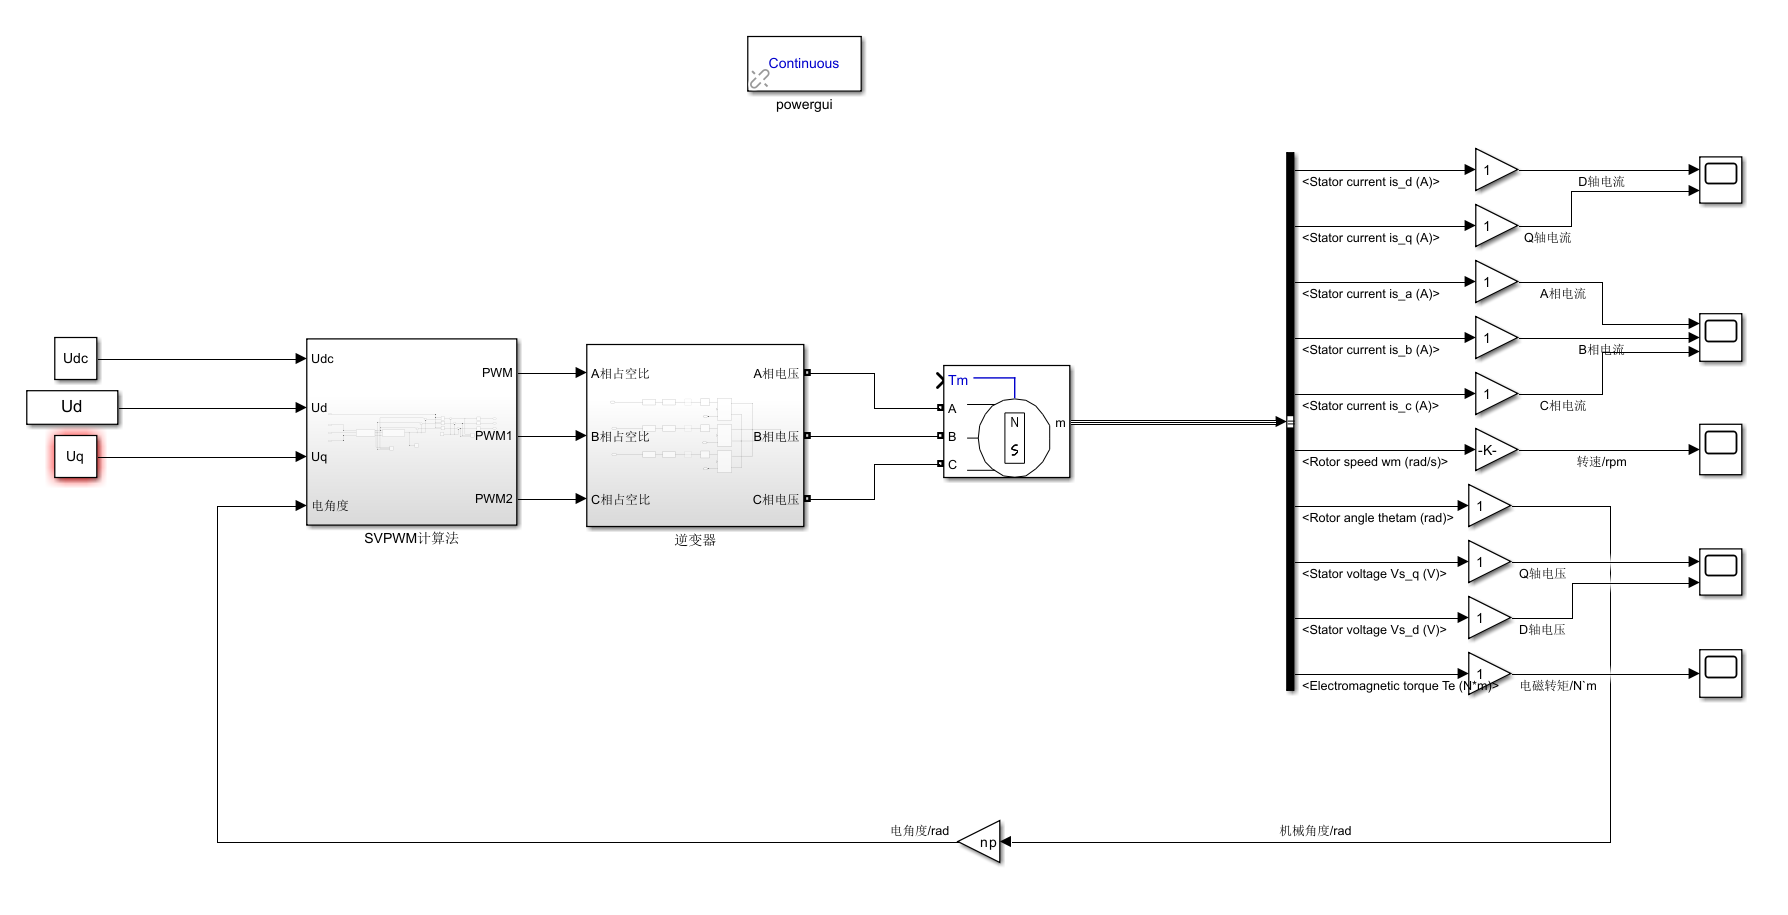
\includegraphics[width=0.8\textwidth]
    {图片/仿真模型.png}
    \caption{仿真模型}
\end{figure}

设定电机参数为相电阻\(R_s=8\Omega\)，同步电感\(L_d=2\)mH，\(L_q=2.5\)mH，永磁体磁链\(\psi_m=0.01\)Wb，极对数\(n_p=14\)，
母线电压\(12\)V。采用SVPWM调制，PWM频率为\(15\)kHz。

对于伪随机信号的选取，选择级数N=11，Hanekel矩阵阶次为8，幅值为1V，采样周期\(T_s=1/15000=66.67\)us。

在系统阶次的选择上，由于理想电路模型本身为一阶，因此系统阶次选取为1。但是PWM和逆变器本身会引入时延，会使得辨识阶次升高至2。接下来对此
简单进行分析。

对于SVPWM调制方法，会引入1拍的延迟，也就是有\(\tau\approx\)66.67us。
根据采用的三相全桥芯片DRV8313数据手册动态特性相关表述，如下所示，DRV8313的行为近似为纯时延+一阶惯性环节。
\begin{figure}[H]
    \centering
    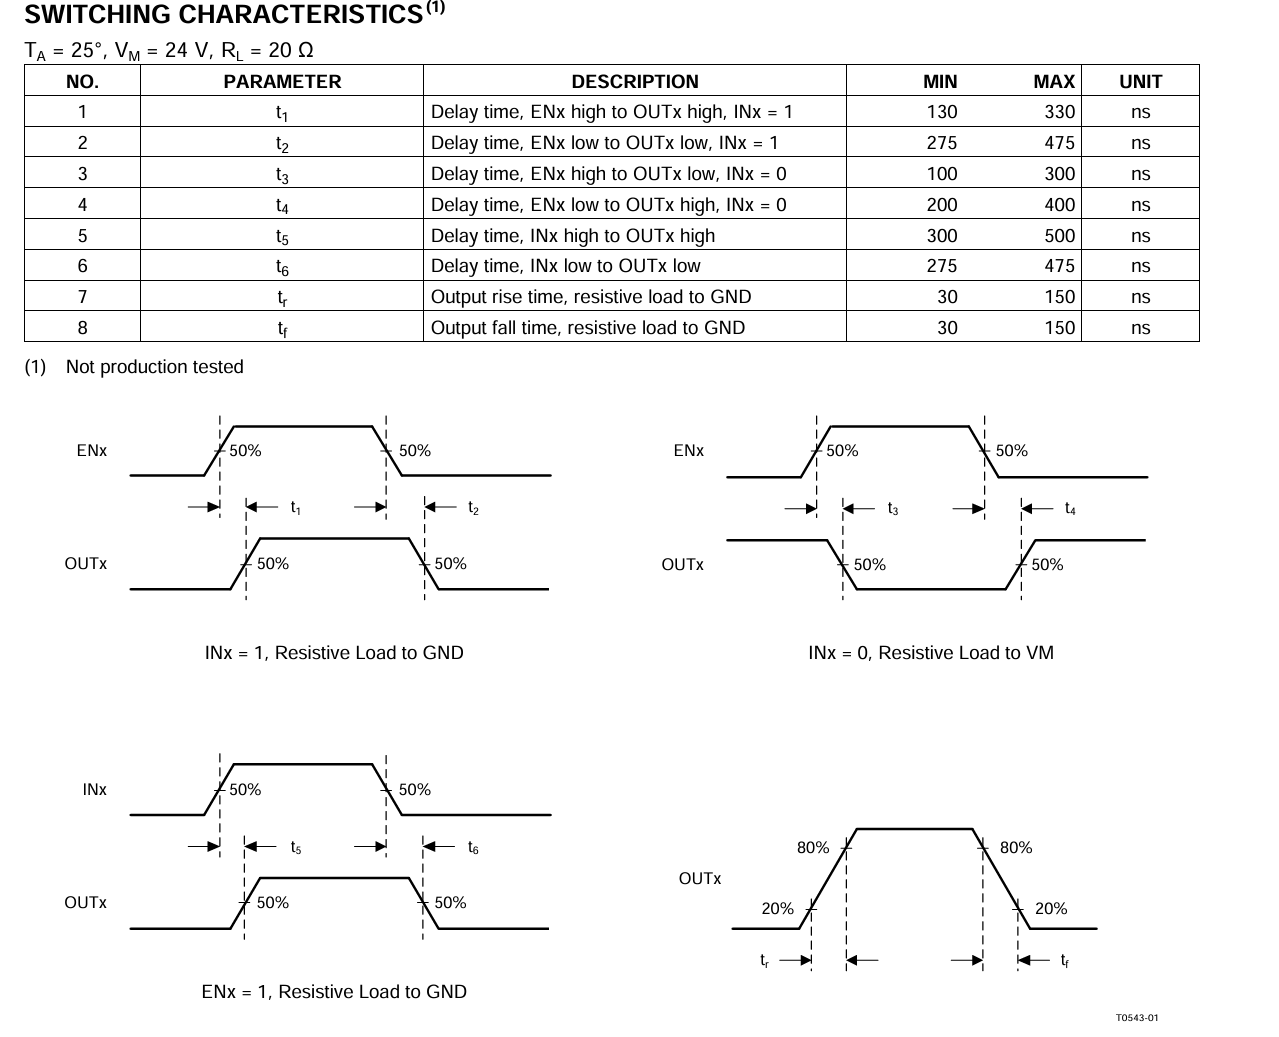
\includegraphics[width=0.8\textwidth]
    {图片/DRV8313动态特性.png}
    \caption{DRV8313动态特性}
\end{figure}

用示波器测量PWM输出信号和逆变器输出时序波形如下图所示。分析可知DRV8313时延时间约260ns，时间常数约120ns。
\begin{figure}[H]
    \begin{minipage}{0.5\textwidth}
        \centering
        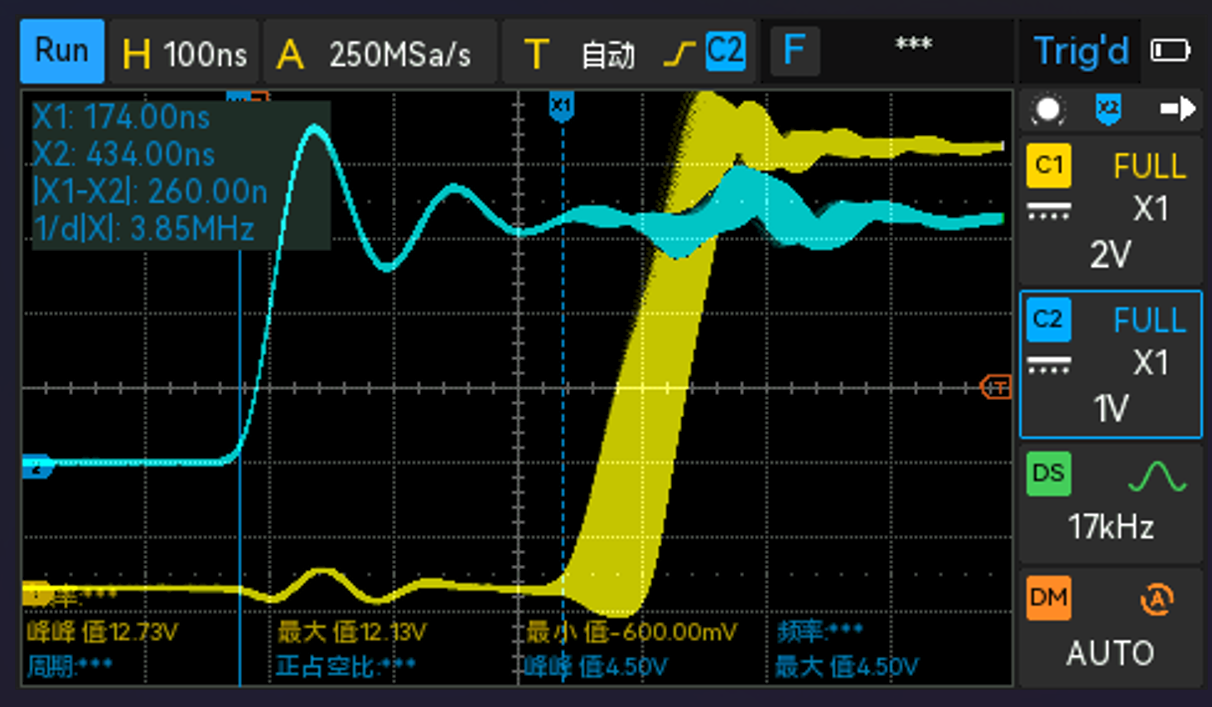
\includegraphics[width=\textwidth]
        {图片/DRV8313动态特性波形图（延时测量）.png}
        \caption{DRV8313逆变器输出时序波形（延时）}
    \end{minipage}
    \begin{minipage}{0.5\textwidth}
        \centering
        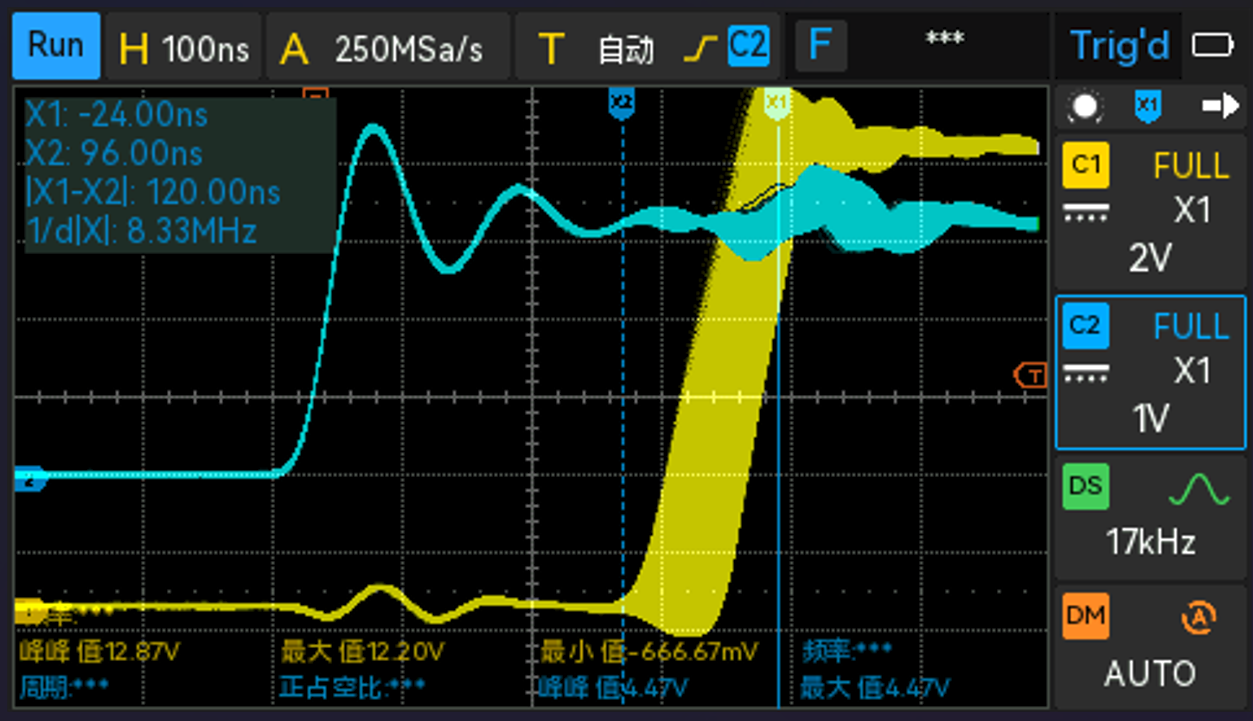
\includegraphics[width=\textwidth]
        {图片/DRV8313动态特性波形图（惯性测量）.png}
        \caption{DRV8313逆变器输出时序波形（惯性）}
    \end{minipage}
\end{figure}

因此PWM和逆变器的传递函数可以表示为：
\begin{equation*}
    \begin{aligned}
        G(s)&=e^{-(66.67\times10^{-6})s}\times e^{-(260\times 10^{-9})s}
        \cfrac{1}{120\times 10^{-9}s+1}\\
        &=e^{-66.93\times10^{-6}s}\cfrac{1}{120\times 10^{-9}s+1}
    \end{aligned}
\end{equation*}

此时整体的被控对象可以表示为\(G(s)=\cfrac{1}{R+Ls}\times\cfrac{1}{120\times 10^{-9}s+1}
\times e^{-66.93\times10^{-6}s}\)，而采样周期\(T_s = 66.67\times 10^{-6}\)s，存在分数拍滞后，
需要用修正Z变换分析其在离散域中的传递函数。但根据Z变换的相关知识可知，修正Z变换只会引起零点和直流
增益的变化。此外，如果只关注极点，则\(\mathcal{Z}[G_1(s)G_2(s)]\)和\(\mathcal{Z}[G_1(s)]\mathcal{
G_2(s)}\)的极点是一致的。因此尽管考虑PWM和逆变器带来的滞后，对于同步电感的辨识仍可以用
\(L_d=-\cfrac{T_sR_s}{\ln(z_{pD})}\)和\(L_q=-\cfrac{T_sR_s}{\ln(z_{pQ})}\)来计算。只是由于
PWM和逆变器带来的非理想因素会导致系统阶次升高，引入极高频的快极点，此时需要进行极点模态分离。

在仿真模型中，用PWM初始延迟模拟PWM的一拍滞后，用时延+惯性环节模拟逆变器特性，并将其与无时延的结果进行对比。
含时延时系统阶次选择为2阶，不含时延时系统阶次选择为1阶。而对于二阶系统，进行模态分离，选取靠近单位圆的慢极点，
将其视为电机本身Q轴电路的模态，而靠近原点的极点视为PWM和逆变器时延引入的模态。

此外，为了模拟实际的非理想因素，还会再输出端引入白噪声模拟采样噪声。后续的仿真分析，将在考虑PWM时延、逆变器惯性
和采样噪声的非理想状态，和不考虑PWM时延、逆变器惯性和采样噪声理想状态都进行分析，并进行对比分析。

\subsubsection{D轴同步电感辨识仿真}

根据电磁转矩表达式\(T_e=\cfrac32pi_qi_d(L_d-L_q)+\cfrac32\psi_mpi_q\)可知，若\(i_q=0\)，则不会产生电磁转矩，电机不会转动，
D轴电路方程可以表示为\(u_d = R_si_d+L_d\cfrac{di_d}{dt}\)。而在零初始条件下，根据电路方程，能够激起\(i_q\)变化的唯一方法是
给定非零的\(u_q\)。因此，只在D轴注入电压，交叉耦合项\(\omega_eL_qi_q=0\)，D轴电路维持为线性定常系统。

首先在理想状态下（不考虑PWM时延、逆变器惯性和采样噪声），在D轴工作点0V附近进行HK辨识仿真，结果如下所示。
\begin{figure}[H]
    \begin{minipage}{0.5\textwidth}
        \centering
        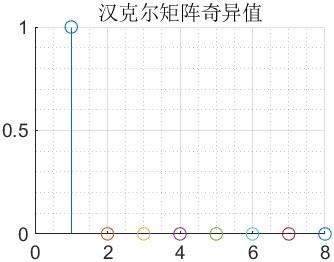
\includegraphics[width=\textwidth]
        {图片/D轴工作点0V归一化奇异值分解图（仿真，理想状态）.jpg}
        \caption{D轴工作点0V归一化奇异值分解图（仿真，理想状态）}
    \end{minipage}
    \begin{minipage}{0.5\textwidth}
        \centering
        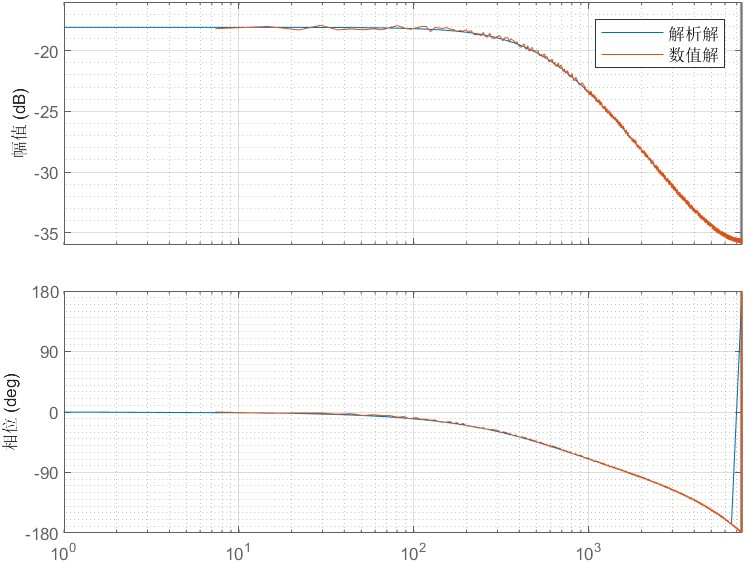
\includegraphics[width=\textwidth]
        {图片/D轴工作点0V解析解与数值解频域对比图（仿真，理想状态）.jpg}
        \caption{D轴工作点0V解析解与数值解频域对比图（仿真，理想状态）}
    \end{minipage}
\end{figure}

可以发现，归一化后的奇异值分解显示系统为一阶，与推导的结果一致。辨识传递函数为：
\begin{equation*}
    G_D(z)=\cfrac{2.125\times 10^{-6} + 0.02916z^{-1}}{1 - 0.7659z^{-1}}
\end{equation*}

数值解与解析解的幅频相关系数
\footnote{皮尔逊相关系数定义为\(r=\cfrac{\sum\limits_{i=1}^n(x_i-\bar{x})(y_i-\bar{y})}
{\sqrt{\sum\limits_{i=1}^n(x_i-\bar{x})^2\sum\limits_{i=1}^n(y_i-\bar{y})^2}}\)，用于描述
两组数据之间的线性相关程度，取值范围为[-1,1]。在一元线性回归中相关系数和决定系数满足\(R^2=r^2\)。
这里衡量的两组原则上一致的数据的线性相关程度，因此相关系数越接近1越好。}
为99.9165\(\%\)，相频相关系数为99.99136\(\%\)，拟合优度
\footnote{拟合优度定义为\(\textrm{BFT}=1-\cfrac{\|y-\hat{y}\|}{\|y-\bar{y}\|}\)，
其中\(y\)表示实测数据，\(\hat{y}\)表示仿真和估测数据，而\(\|\cdot\|\)表示欧几里得范数，对于实数向量
计算为\(\|x\|=\sqrt{\sum\limits_{i=1}^nx_i^2}\)，
对于复数则计算为\(\|z\|=\sqrt{\sum\limits_{i=1}^n|z_i|^2}\)，相较于相关系数，拟合优度
能够反映两组数据的一致性，对直流偏置、线性增益有敏感性，同样也是越接近1两组数据的一致性越高。}
97.49761\(\%\)，
拟合程度极高。
解析解极点位于\(z_{pD}=0.7659\)处，根据\(L_d=-\cfrac{T_sR_s}{\ln(z_{pD})}\)
得到辨识结果\(L_d=1.99946\)mH，相对误差-0.02699\(\%\)。

用同样的方法，从-5V到5V，以0.1V为步长进行辨识，辨识结果如下图所示：
\begin{figure}[H]
    \centering
    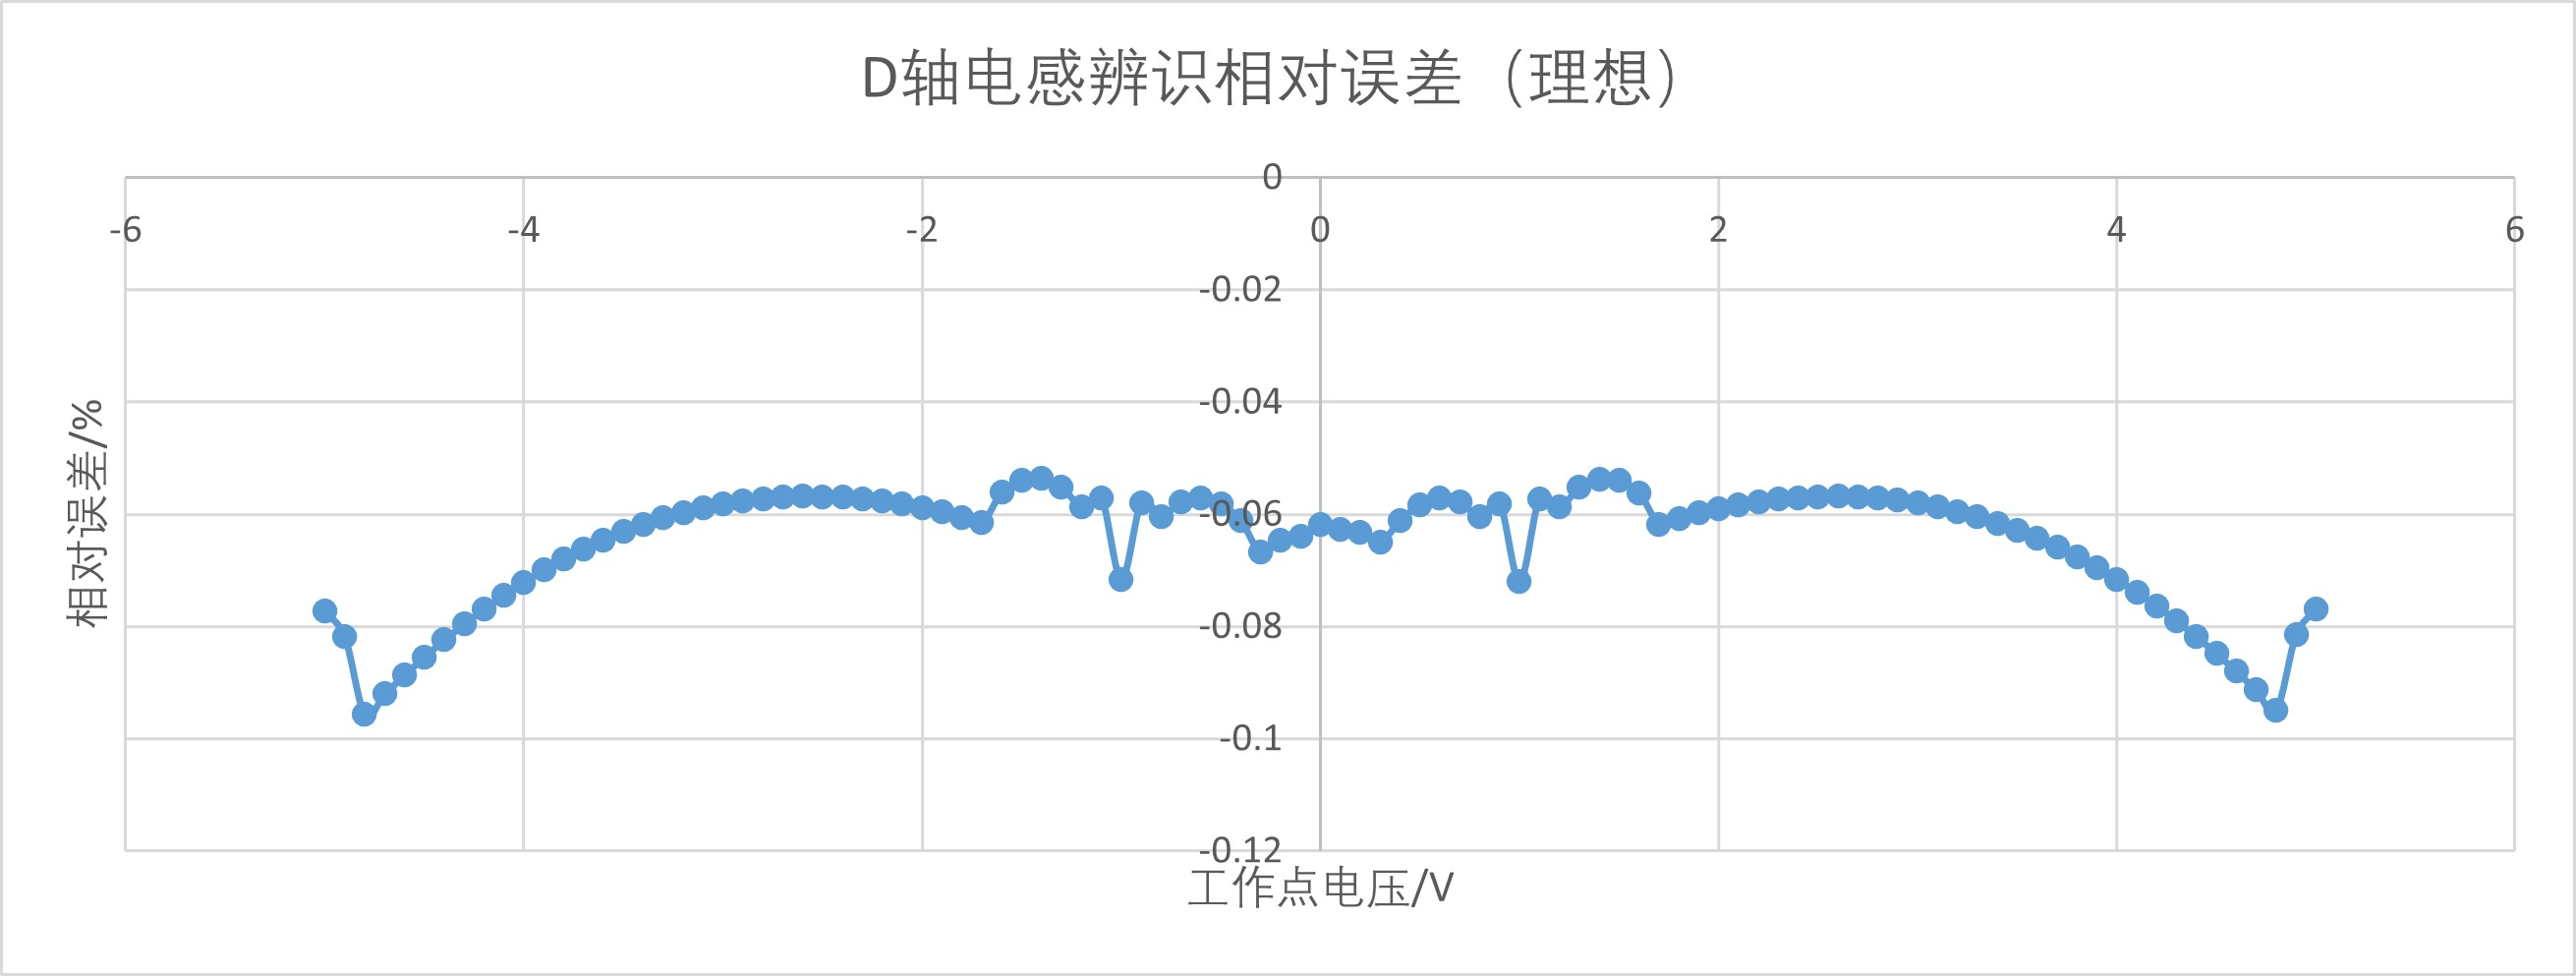
\includegraphics[width=0.8\textwidth]
    {图片/D轴工作点相对误差分析（仿真，理想状态）.jpg}
    \caption{D轴工作点相对误差分析（仿真，理想状态）}
\end{figure}

分析数据可知，在没有时延的仿真环境下，相对误差最大不超过0.07\(\%\)，辨识精度极高。

接下来考虑引入PWM时延、逆变器惯性和采样噪声的非理想情况，进行HK辨识仿真。结果如下：
\begin{figure}[H]
    \begin{minipage}{0.5\textwidth}
        \centering
        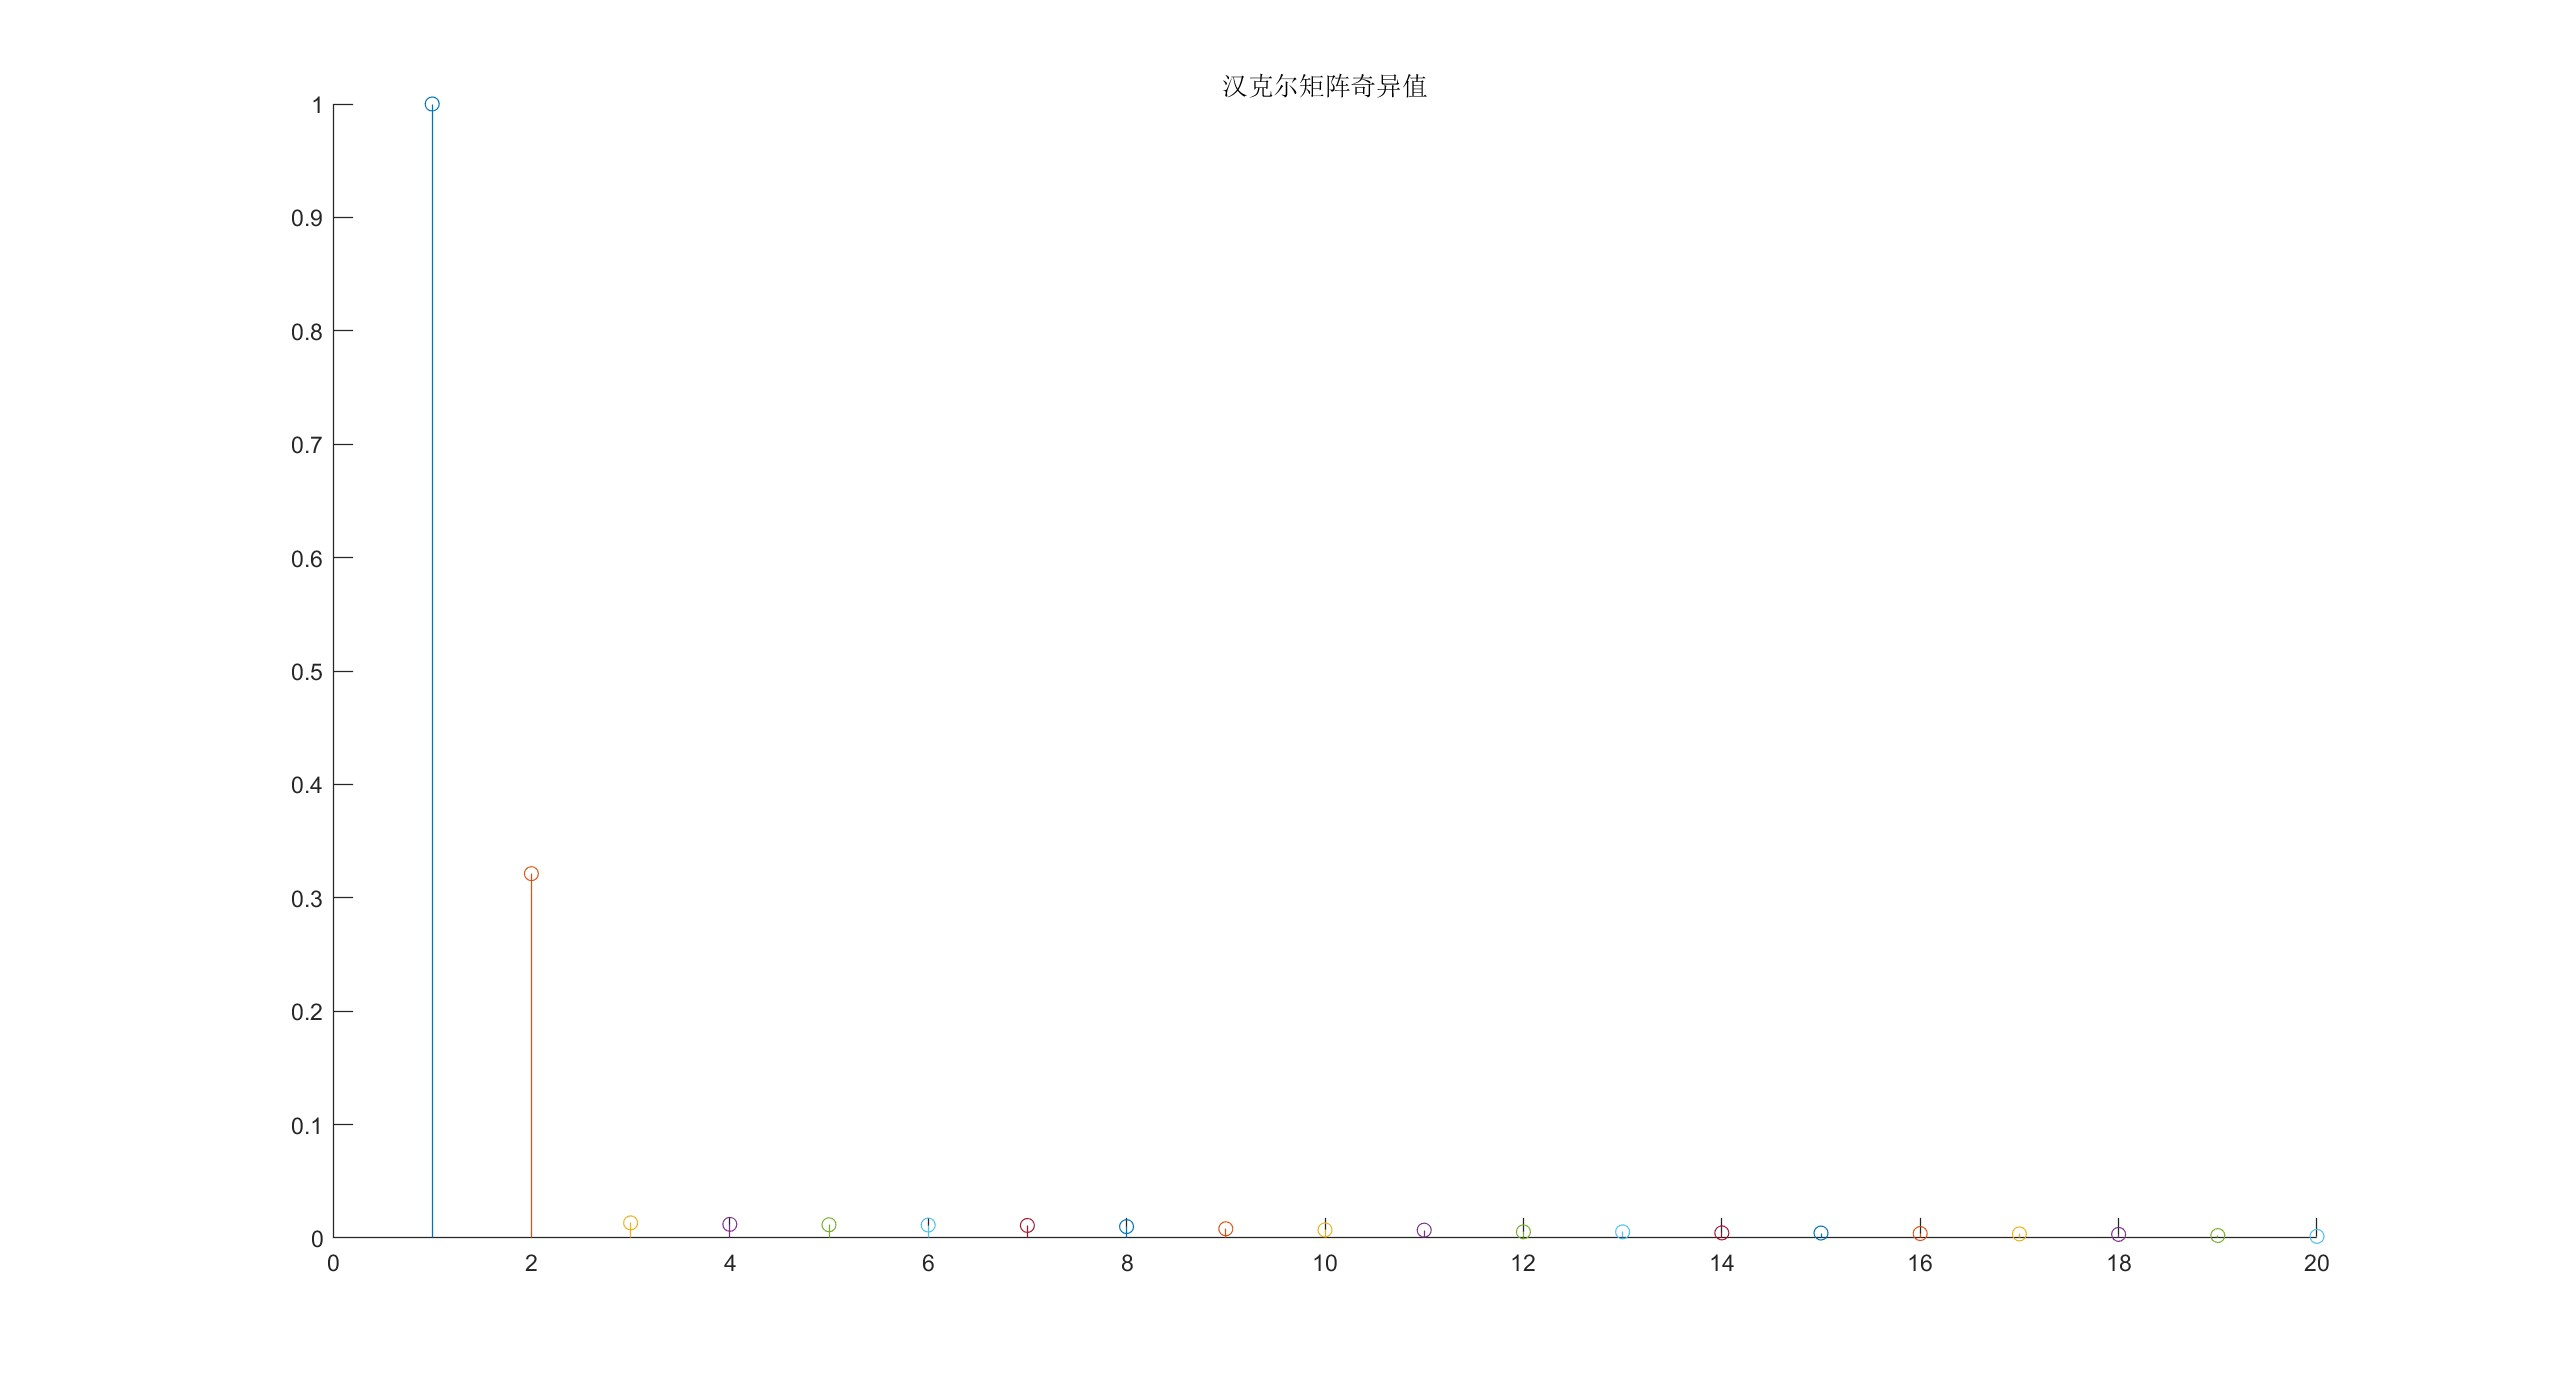
\includegraphics[width=\textwidth]
        {图片/D轴工作点0V归一化奇异值分解图（仿真，非理想状态）.jpg}
        \caption{D轴工作点0V归一化奇异值分解图（仿真，非理想状态）}
    \end{minipage}
    \begin{minipage}{0.5\textwidth}
        \centering
        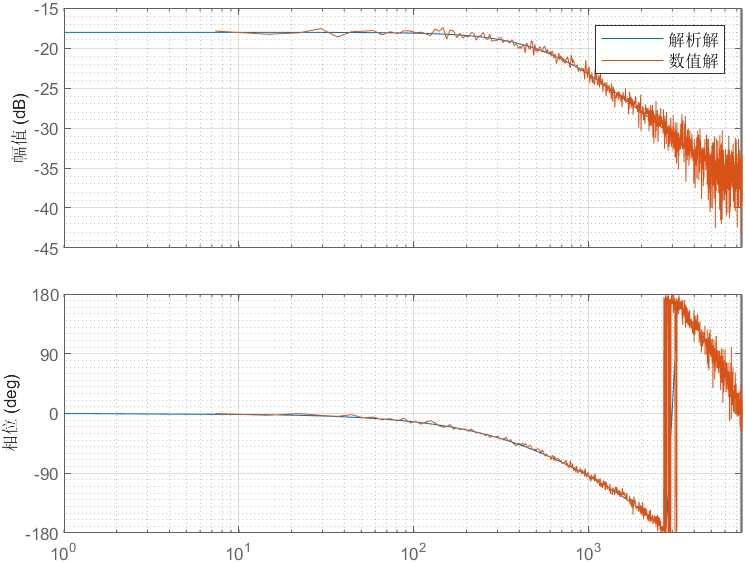
\includegraphics[width=\textwidth]
        {图片/D轴工作点0V解析解与数值解频域对比图（仿真，非理想状态）.jpg}
        \caption{D轴工作点0V解析解与数值解频域对比图（仿真，非理想状态）}
    \end{minipage}
\end{figure}

可以发现，归一化后的奇异值分解显示系统为二阶，这是PWM时延与逆变器惯性导致的结果。辨识传递函数为：
\begin{equation*}
    G_D(z)=\cfrac{-0.0005905 + 0.0006895z^{-1}+0.02919z^{-2}}{1 - 0.7704z^{-1} + 0.004188z^{-2}}
\end{equation*}

数值解与解析解的幅频相关系数为98.91053\(\%\)，相频相关系数为99.81401\(\%\)，拟合优度87.16411\(\%\)
拟合程度相较于无时延有一定的下降（尤其是拟合优度），但整体仍处于较高拟合程度。
解析解极点位于\(z_{pD}=0.7649,0.0055\)处，根据\(L_d=-\cfrac{T_sR_s}{\ln(z_{pD})}\)，选取靠近单位圆的\(z_{pD}=0.7669\)为
电机本身的模态，得到辨识结果\(L_d=1.99010\)mH，相对误差-0.49494\(\%\)，相对误差有所上升。

同样从-5V到5V，以0.1V为步长进行辨识，辨识结果如下图所示：
\begin{figure}[H]
    \centering
    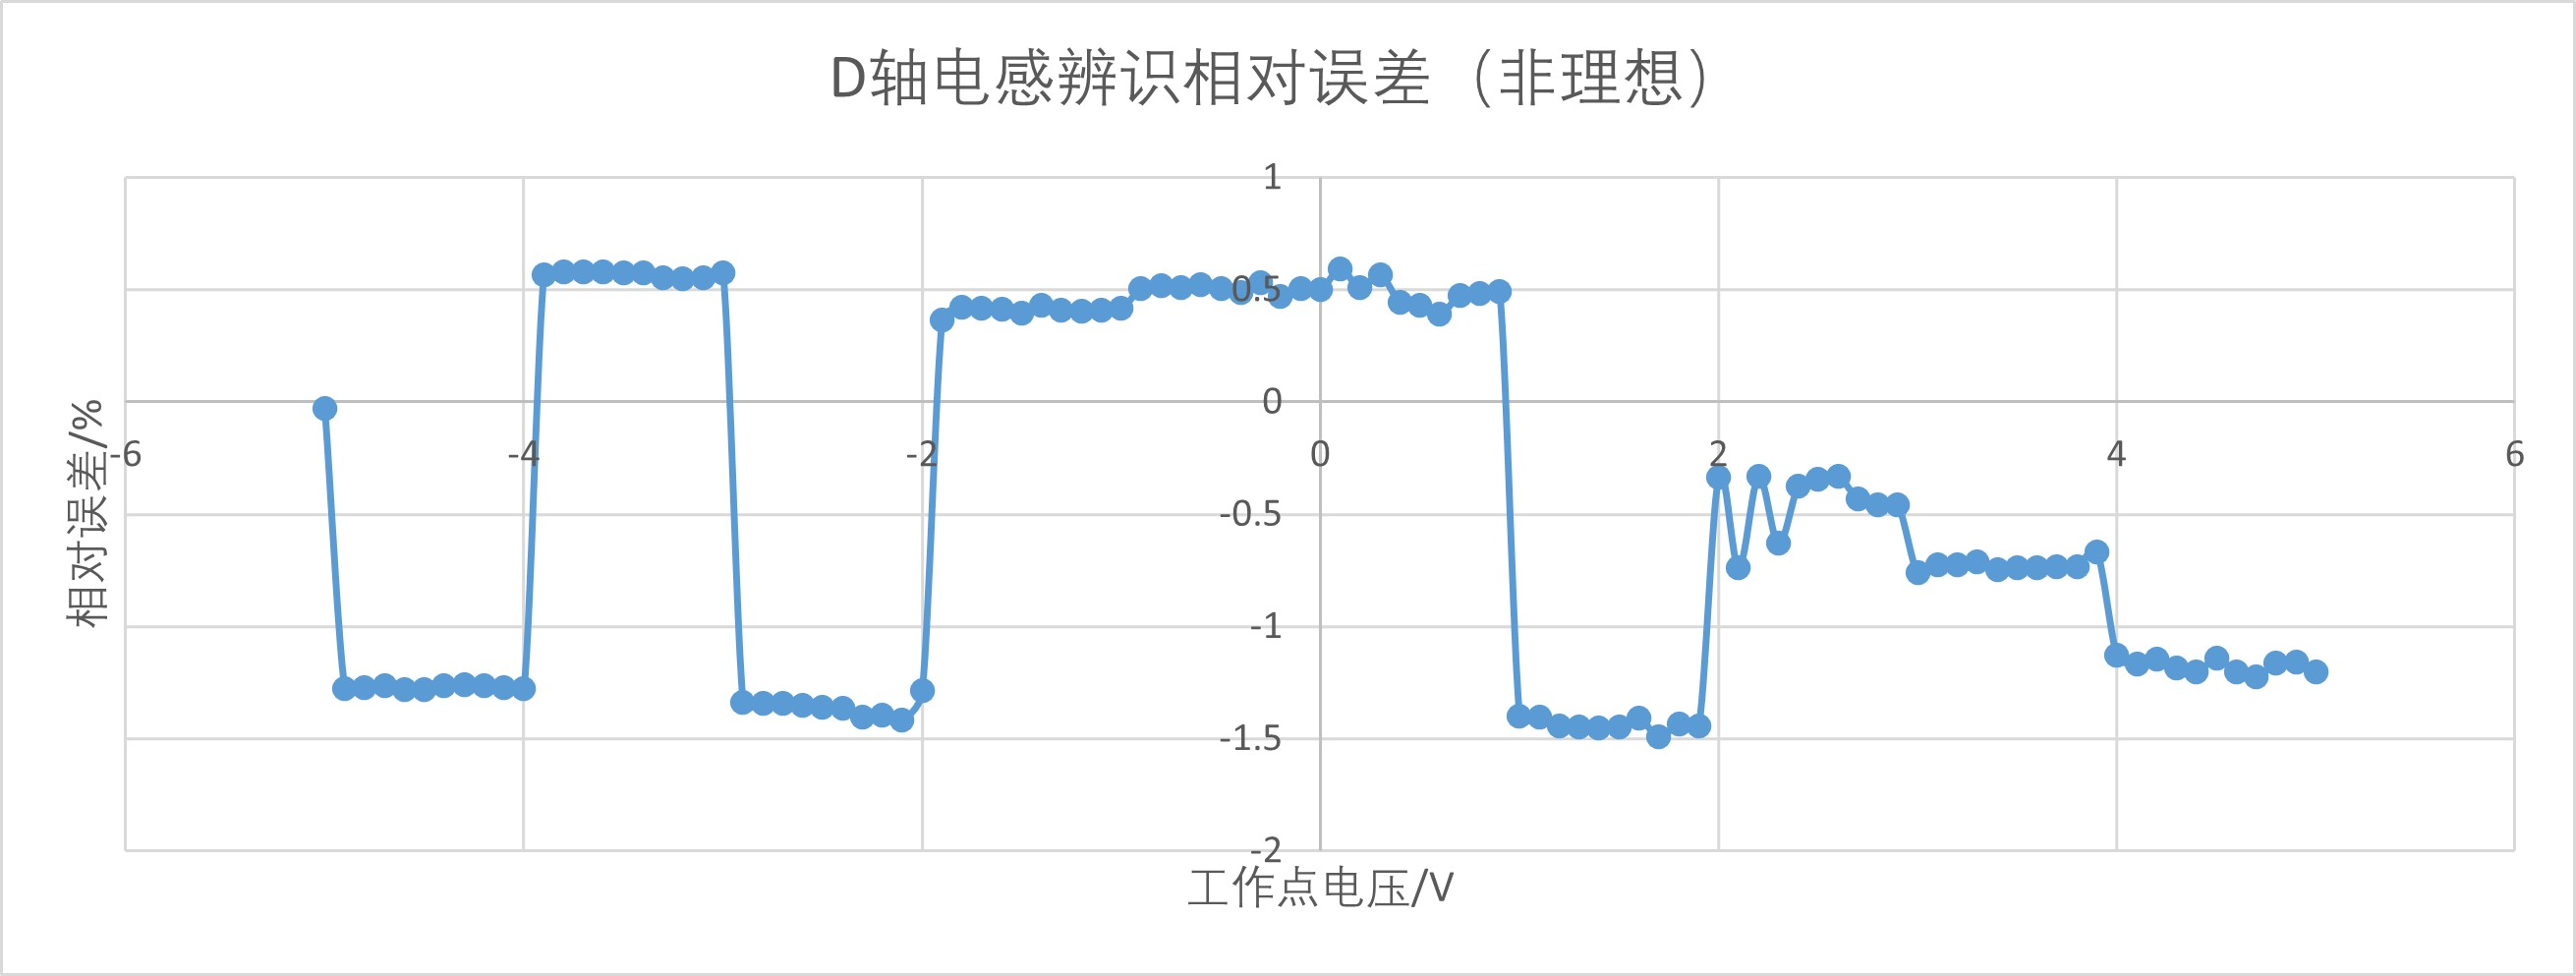
\includegraphics[width=0.8\textwidth]
    {图片/D轴工作点相对误差分析（仿真，非理想状态）.jpg}
    \caption{D轴工作点相对误差分析（仿真，非理想状态）}
\end{figure}

分析数据可知，在含有时延的仿真环境下，相对误差最大超过了3\(\%\)，辨识精度相较于无时延有所下降，但仍处于可接受范围内。分析造成
相对误差增大的原因主要一是PWM时延、逆变器惯性和采样噪声等非理想因素降低了信噪比，影响了辨识精度。

\subsubsection{Q轴同步电感辨识仿真}

根据Q轴电路方程：
\begin{equation*}
    u_q=R_si_q+L_d\cfrac{di_q}{dt}+\omega_e(L_di_d+\psi_m)
\end{equation*}

若要消除交叉耦合，则可以通过电气或机械锁轴使得
\(\omega_e=0\)实现。但实测发现电气锁轴或机械堵转都难以彻底消除微动，交叉耦合项难以完全抵消（详见\ref{sec:电气锁轴方法}
和\ref{sec:机械堵转方法}）。因此最终选择进行数据后处理方法。

根据Q轴电路方程，可以变形得到：
\begin{equation*}
    u_q-\omega_e(L_di_d+\psi_m)=R_si_q+L_q\cfrac{di_q}{dt}
\end{equation*}

因此，通过实时记录某一拍的\(u_q,\omega_e,i_d,i_q\)，结合\(L_d,R_s,\psi_m\)的辨识结果，可以将运动耦合项完全补偿，
得到实际上给定Q轴RL电路的输入信号为\(u_q'=u_q-\omega_e(L_di_d+\psi_m)\)，
此时传递函数为\(G_Q(s)=\cfrac{I_q(s)}{U_q'(s)}=\cfrac{1}{R_s+sL_q}\)（其中永磁体磁链的辨识依赖于稳态模型，不包含复杂的信号处理，
详见\ref{sec:永磁体磁链测量}）。

与D轴类似，首先不考虑PWM和逆变器的时延，在0V工作点附近进行HK辨识，结果如下：
\begin{figure}[H]
    \begin{minipage}{0.5\textwidth}
        \centering
        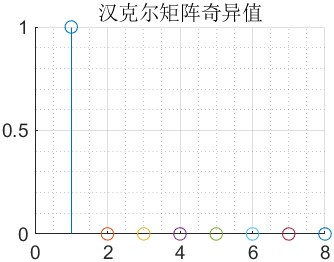
\includegraphics[width=\textwidth]
        {图片/Q轴工作点0V归一化奇异值分解图（仿真，理想状态）.jpg}
        \caption{Q轴工作点0V归一化奇异值分解图（仿真，理想状态）}
    \end{minipage}
    \begin{minipage}{0.5\textwidth}
        \centering
        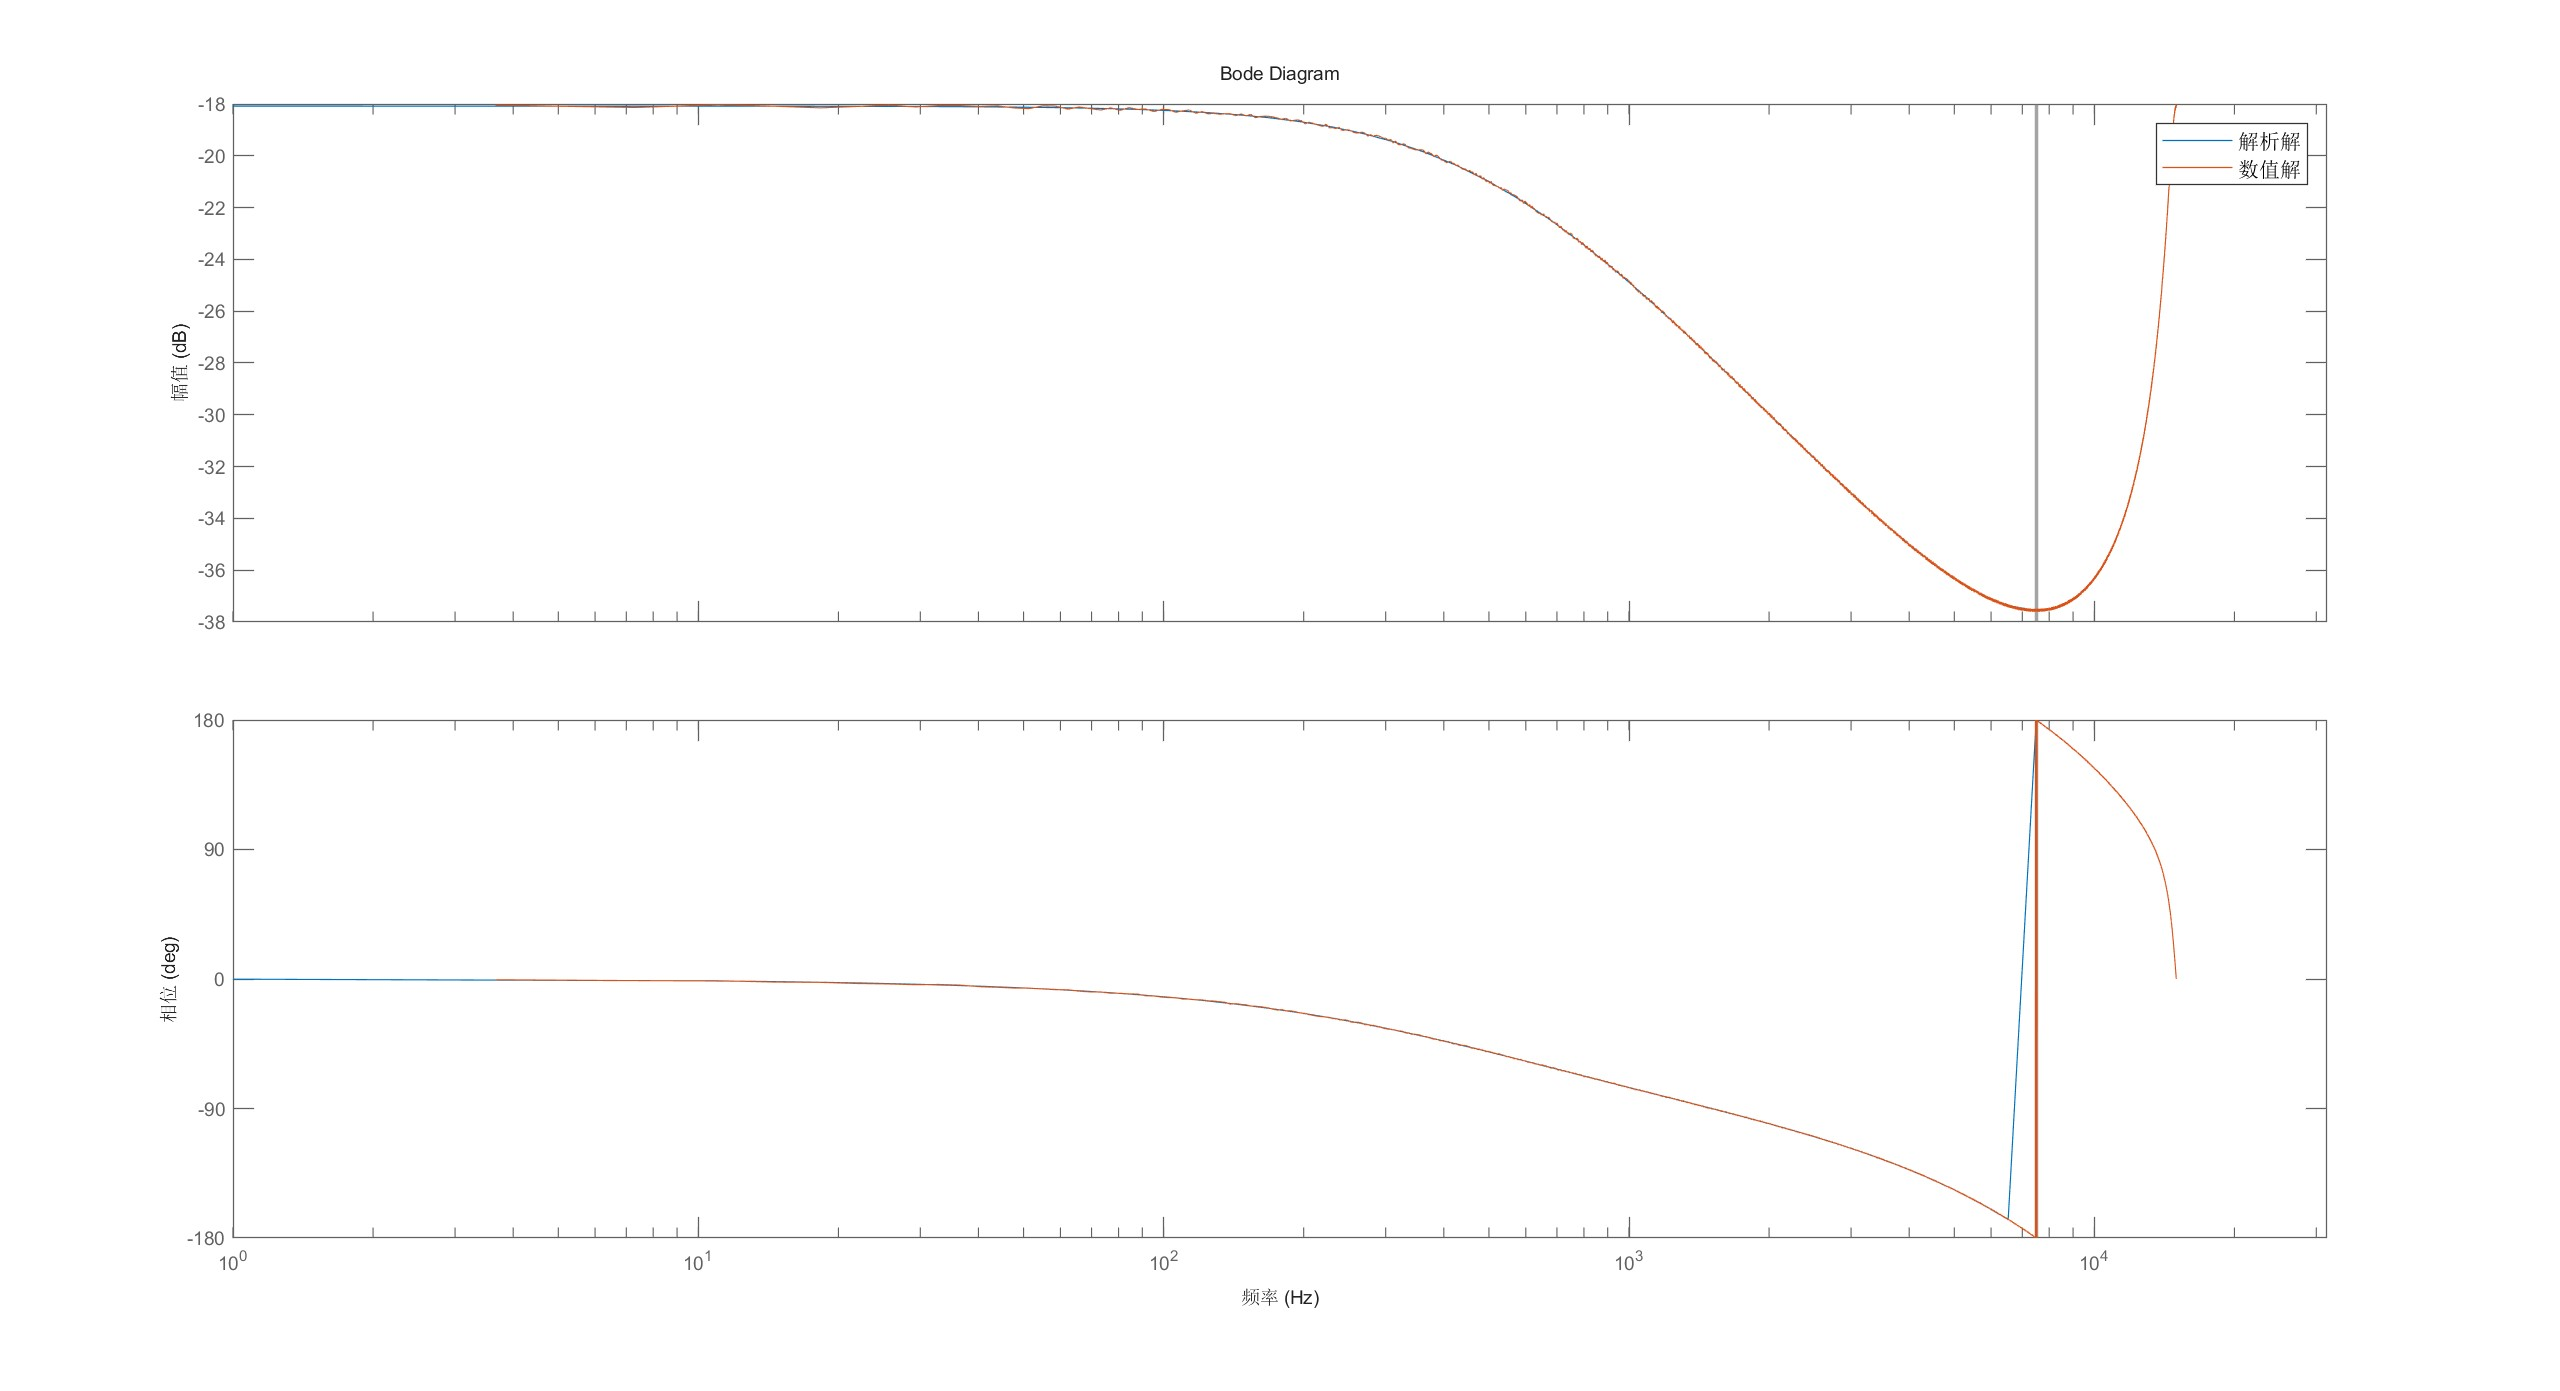
\includegraphics[width=\textwidth]
        {图片/Q轴工作点0V解析解与数值解频域对比图（仿真，理想状态）.jpg}
        \caption{Q轴工作点0V解析解与数值解频域对比图（仿真，理想状态）}
    \end{minipage}
\end{figure}

系统阶次为一阶，辨识传递函数为：
\begin{equation*}
    G_Q(z)=\cfrac{1.834\times 10^{-5} + 0.02396z^{-1}}{1 - 0.8078z^{-1}}
\end{equation*}

数值解与解析解的幅频相关系数为99.96727\(\%\)，相频相关系数为99.99104\(\%\)，
拟合优度97.46235\(\%\)，拟合程度极高。
解析解极点位于\(z_{pQ}=0.8078\)处，根据\(L_q=-\cfrac{T_sR_s}{\ln(z_{pQ})}\)
得到辨识结果\(L_q=2.49837\)mH，相对误差-0.06524\(\%\)。

用同样的方法，从-5V到5V，以0.1V为步长进行辨识，辨识结果如下图所示：
\begin{figure}[H]
    \centering
    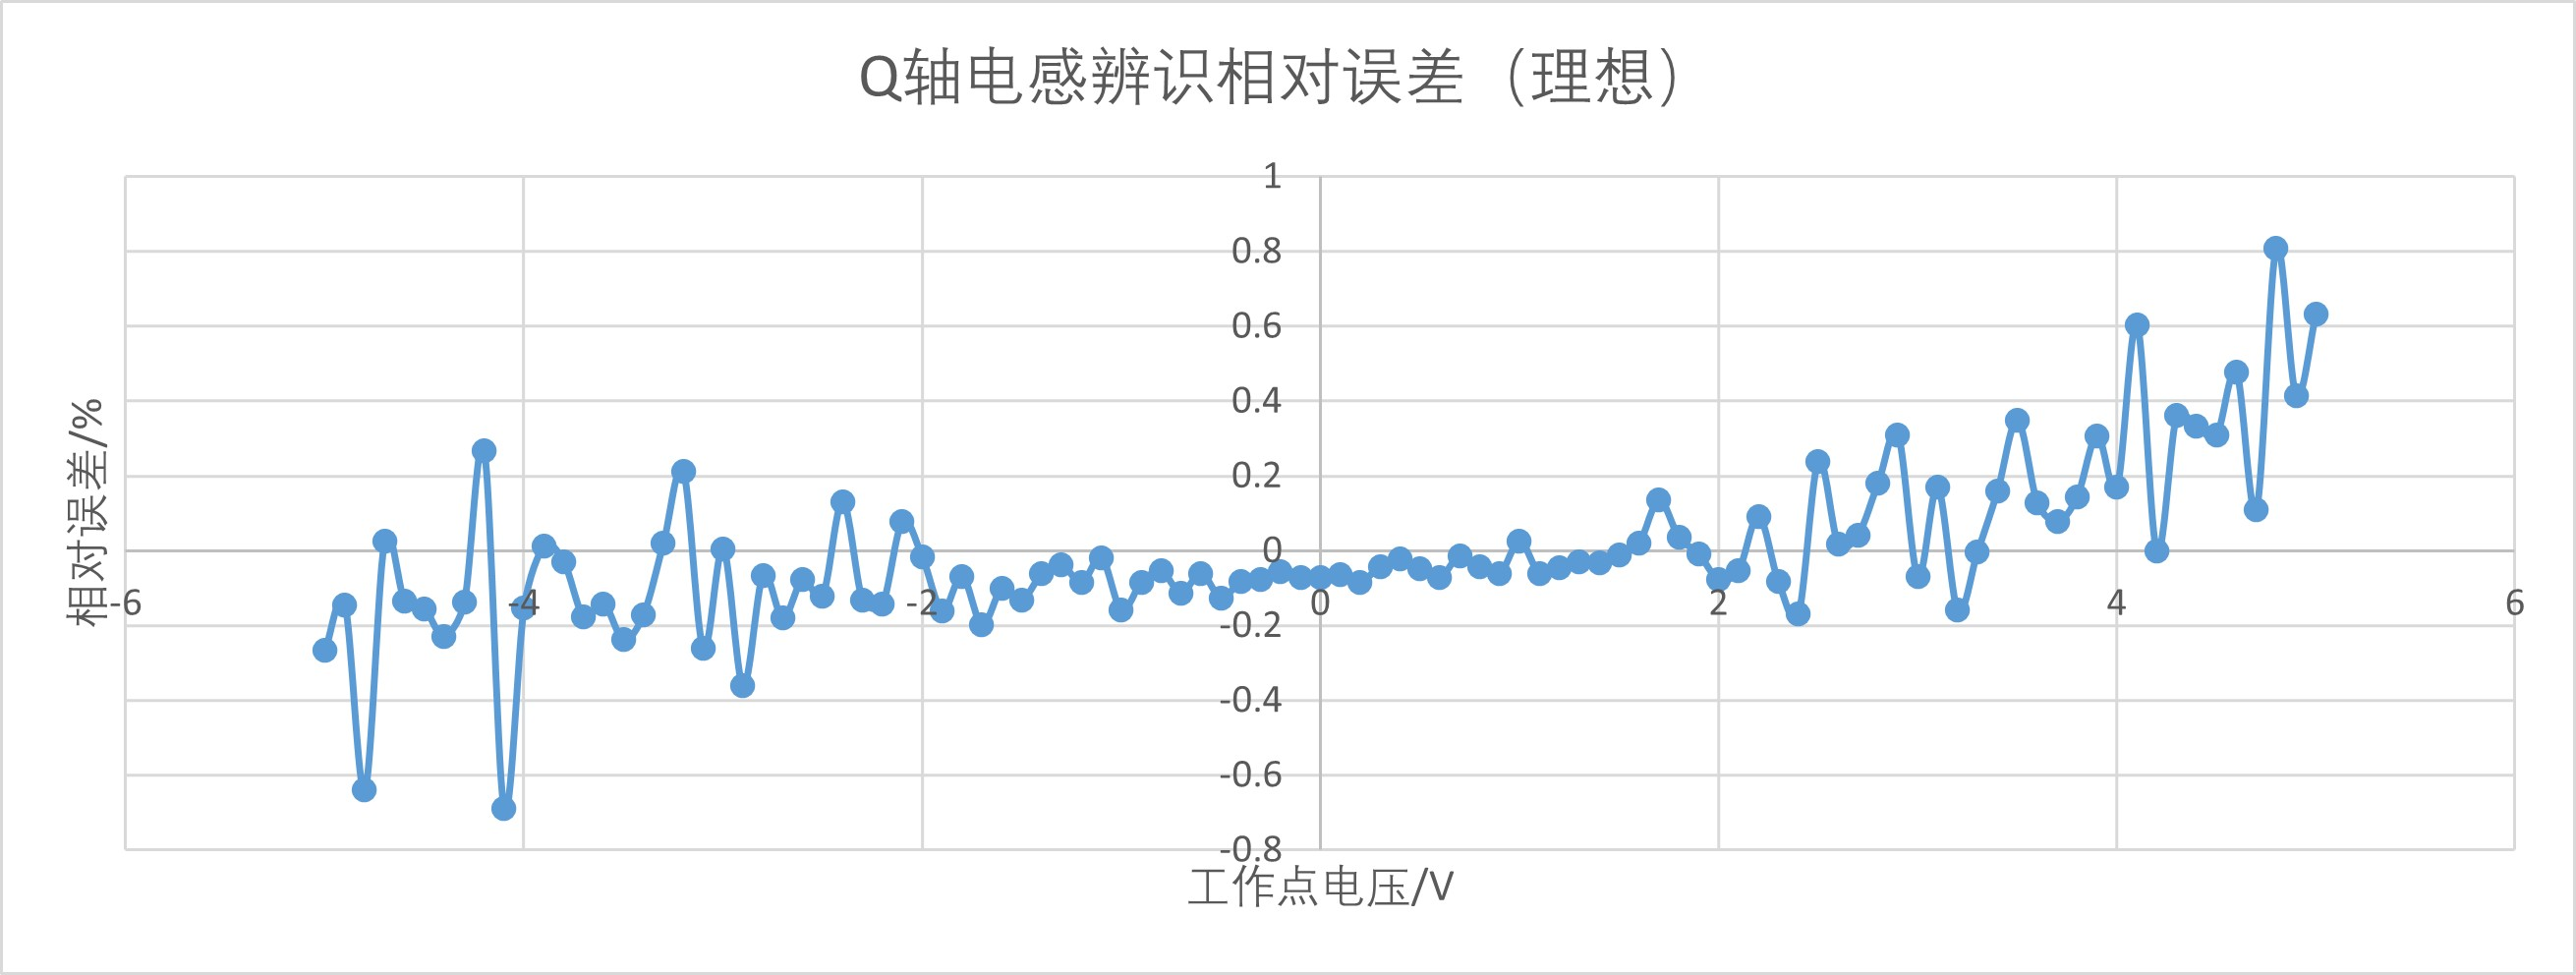
\includegraphics[width=0.8\textwidth]
    {图片/Q轴工作点相对误差分析（仿真，理想状态）.jpg}
    \caption{Q轴工作点相对误差分析（仿真，理想状态）}
\end{figure}

在没有时延的仿真环境下，相对误差最大不超过1\(\%\)，同样具有较高的辨识精度。

接下来在非理想状态下，进行Q轴的HK辨识，在0V工作点附近的辨识结果如下：
\begin{figure}[H]
    \begin{minipage}{0.5\textwidth}
        \centering
        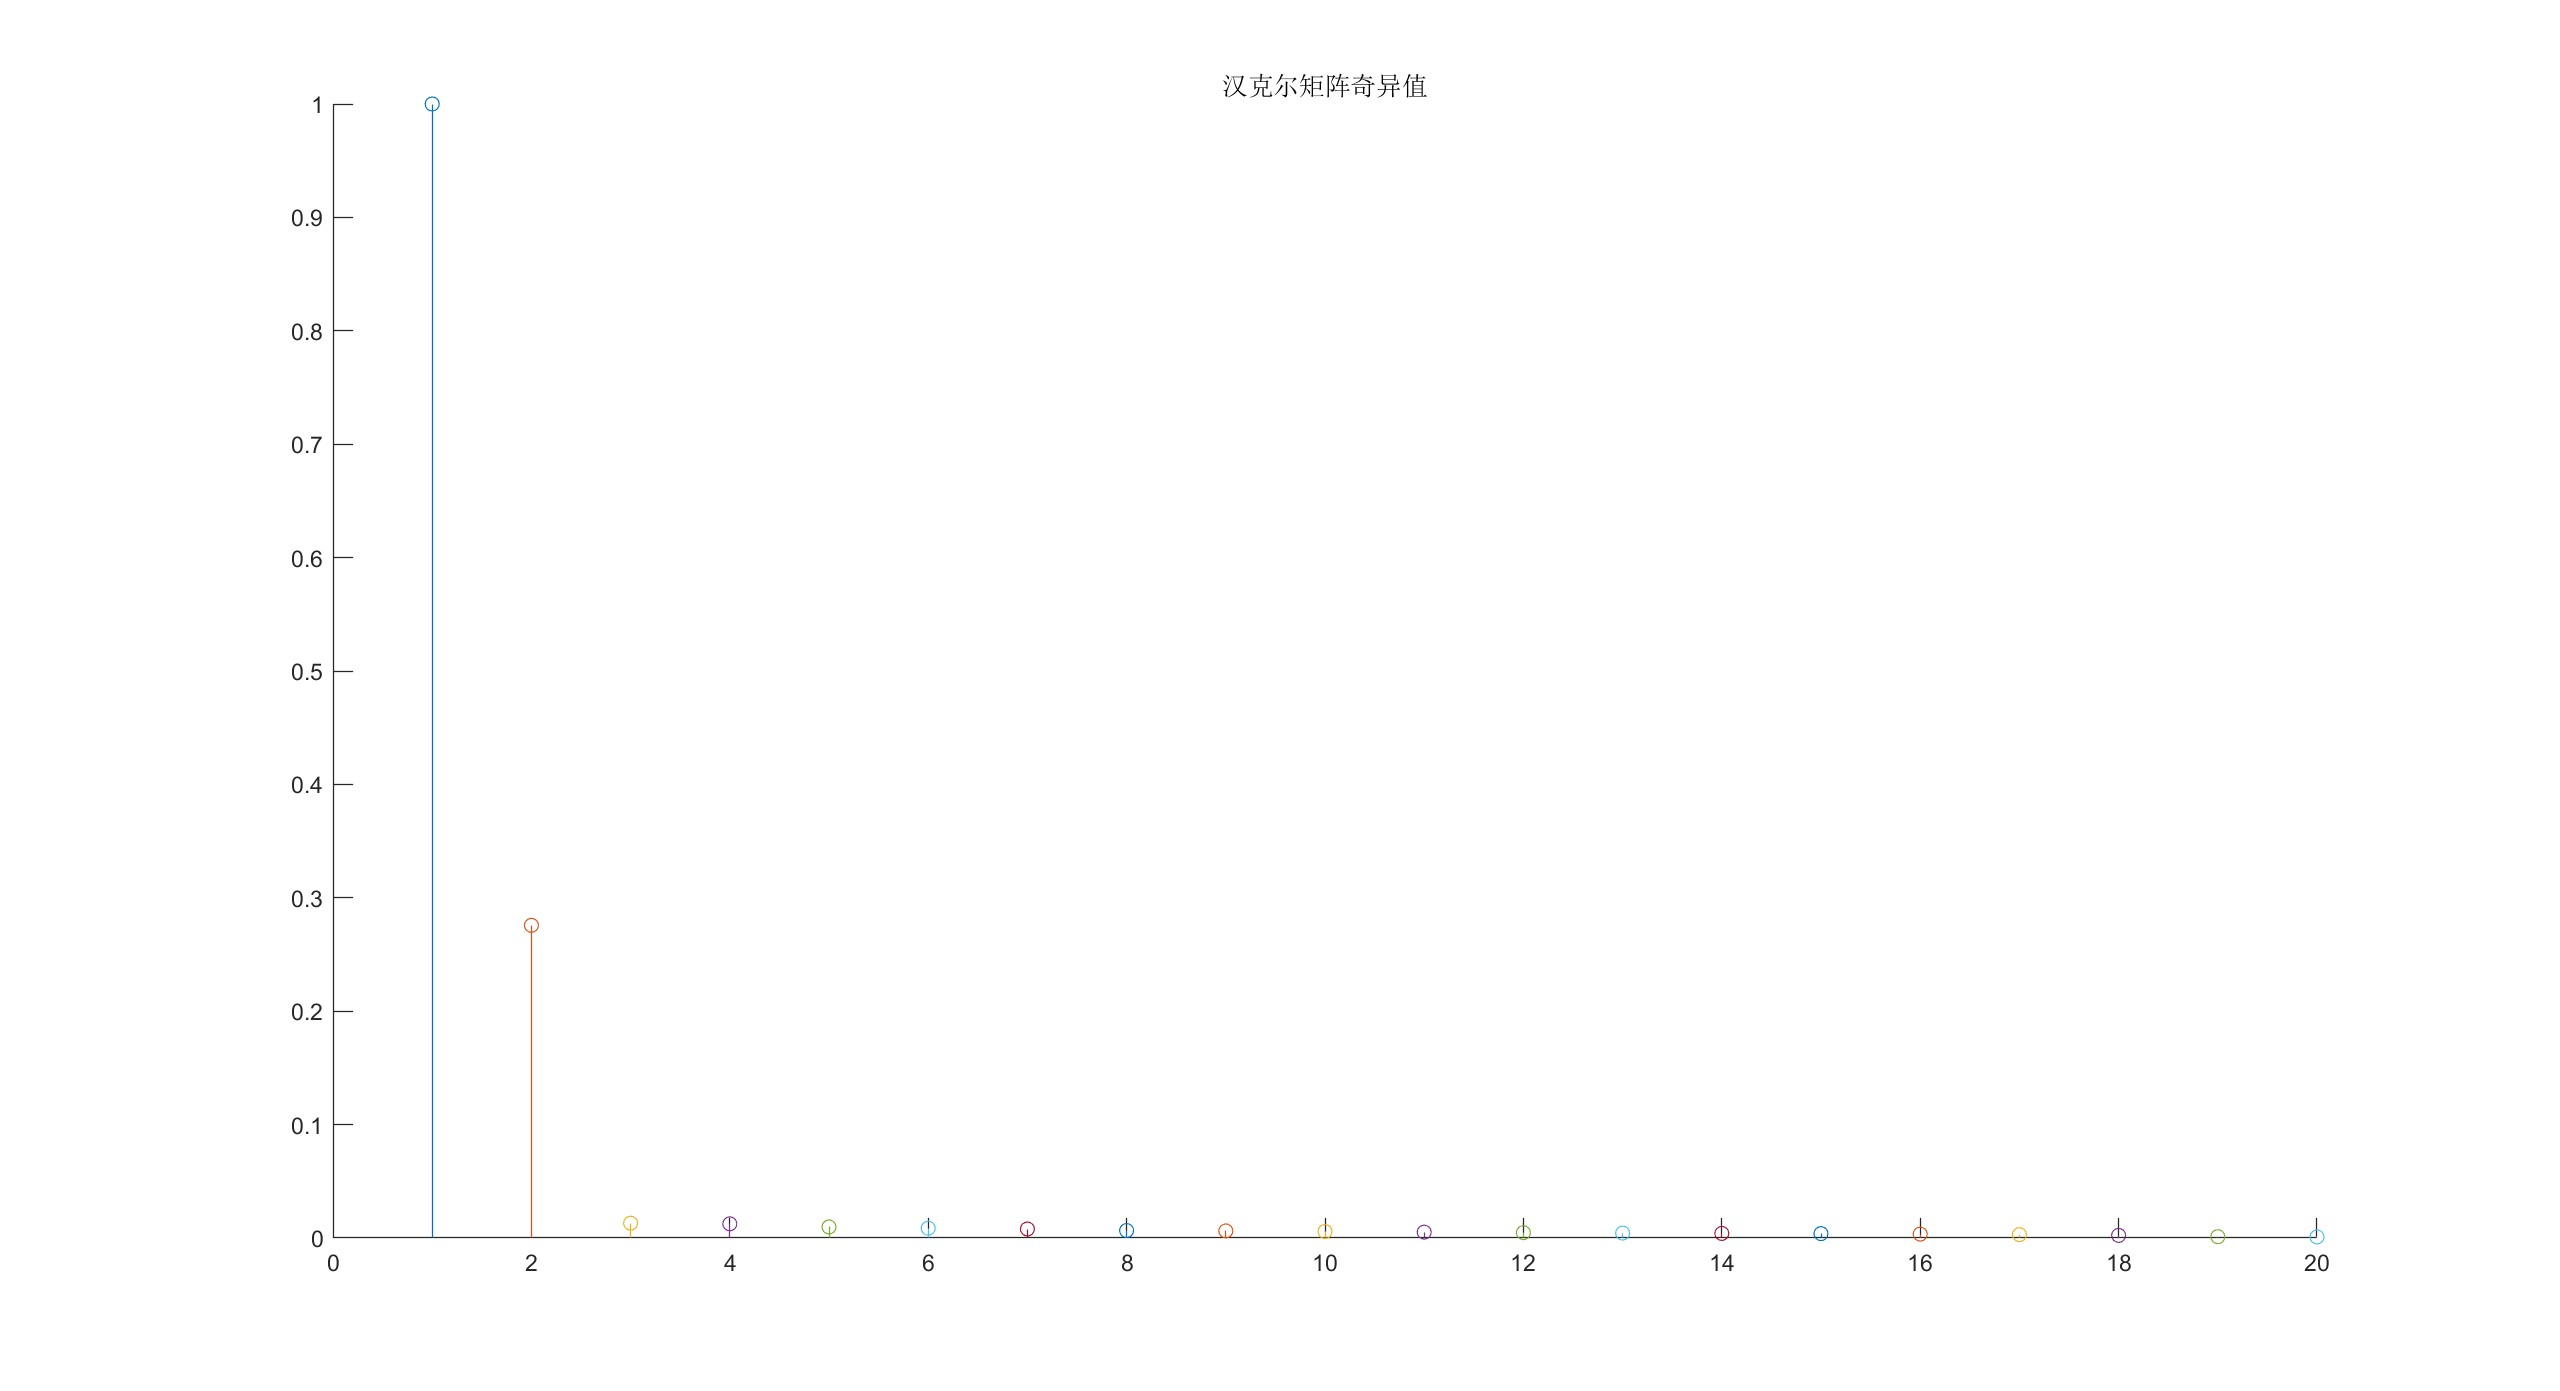
\includegraphics[width=\textwidth]
        {图片/Q轴工作点0V归一化奇异值分解图（仿真，非理想状态）.jpg}
        \caption{Q轴工作点0V归一化奇异值分解图（仿真，非理想状态）}
    \end{minipage}
    \begin{minipage}{0.5\textwidth}
        \centering
        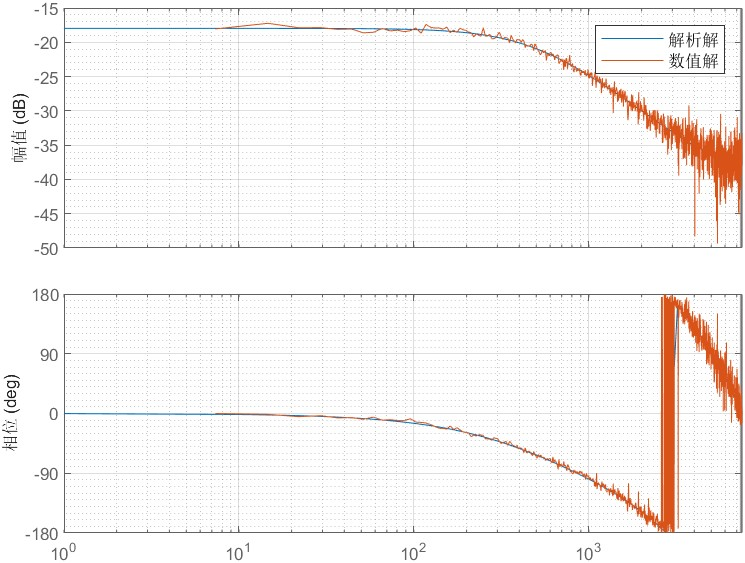
\includegraphics[width=\textwidth]
        {图片/Q轴工作点0V解析解与数值解频域对比图（仿真，非理想状态）.jpg}
        \caption{Q轴工作点0V解析解与数值解频域对比图（仿真，非理想状态）}
    \end{minipage}
\end{figure}

此时由于PWM和逆变器的时延和惯性引入，系统阶次升高到二阶。辨识传递函数为：
\begin{equation*}
    G_Q(z)=\cfrac{-0.0003051 - 0.0001163z^{-1}+0.02413z^{-2}}{1 - 0.8033z^{-1} - 0.007138z^{-2}}
\end{equation*}

数值解与解析解的幅频相关系数为98.98804\(\%\)，相频相关系数为99.74614\(\%\)，
拟合优度86.60122\(\%\)，拟合程度同样降低。
解析解极点位于\(z_{pQ}=0.8092,-0.088\)处，根据\(L_q=-\cfrac{T_sR_s}{\ln(z_{pQ})}\)，选取靠近单位圆的\(z_{pQ}=0.8092\)为
电机本身的模态，得到辨识结果\(L_q=2.51867\)mH，相对误差0.74672\(\%\)，相对误差有所上升。

从-5V到5V，以0.1V为步长进行辨识，辨识结果如下图所示：
\begin{figure}[H]
    \centering
    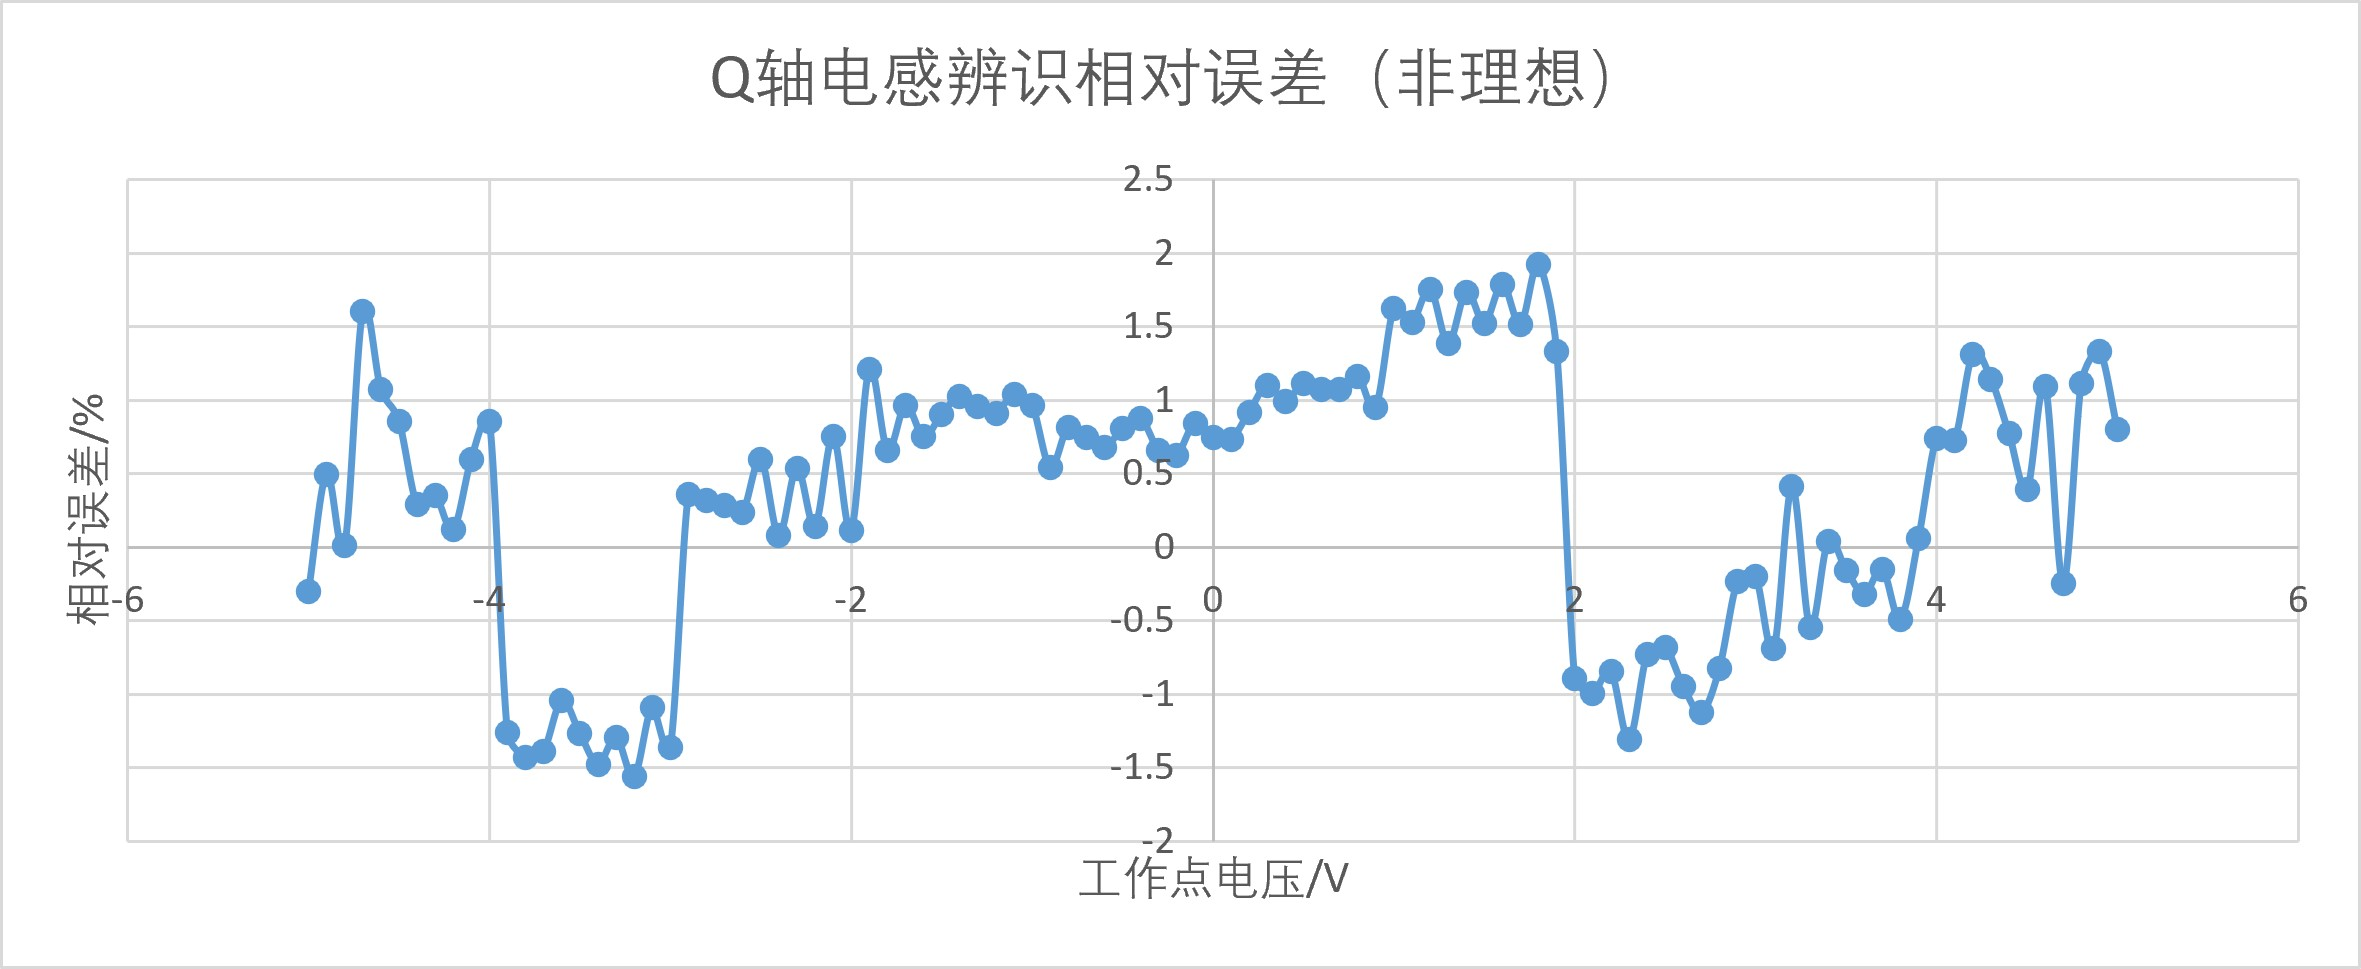
\includegraphics[width=0.8\textwidth]
    {图片/Q轴工作点相对误差分析（仿真，非理想状态）.jpg}
    \caption{Q轴工作点相对误差分析（仿真，非理想状态）}
\end{figure}

在有时延的仿真环境下，辨识精度下降，相对误差升高至2\(\%\)，也在可接受范围内。
相较于D轴，Q轴辨识精度整体较差，分析主要原因就是Q轴的运动解耦并不完全所致。

\subsection{D轴同步电感辨识}

\subsubsection{D轴同步电感辨识过程}

取PWM频率为15kHz，也是电流环控制频率和采样频率。为随机信号级数N=11，伪随机幅值为
1V，在工作点0V、2V、4V、-2V、-4V分别注入伪随机\(u_d\)信号并采集\(i_d\)数据进行分析。

由于串口通信速率有限，这里选择定义输入信号数组\texttt{uint16\(\_\)t m\(\_\)seq[((1 << PRBS\(\_\)N) - 1) * PRBS\(\_\)n];}
和所有需要采集的输出信号数组\texttt{float Output [((1 << PRBS\(\_\)N) - 1) * PRBS\(\_\)n][3];}，在电流控制周期中写入数据，
伪随机信号辨识完成后通过标志位\texttt{bool HK\(\_\)END;}通知速度环控制周期，然后再逐个上传到上位机。

工作点0V，伪随机幅值1V，得到的输入输出曲线、输入自相关函数、输入输出互相关函数、脉冲响应序列如下图所示。
\begin{figure}[H]
    \begin{minipage}{0.5\textwidth}
        \centering
        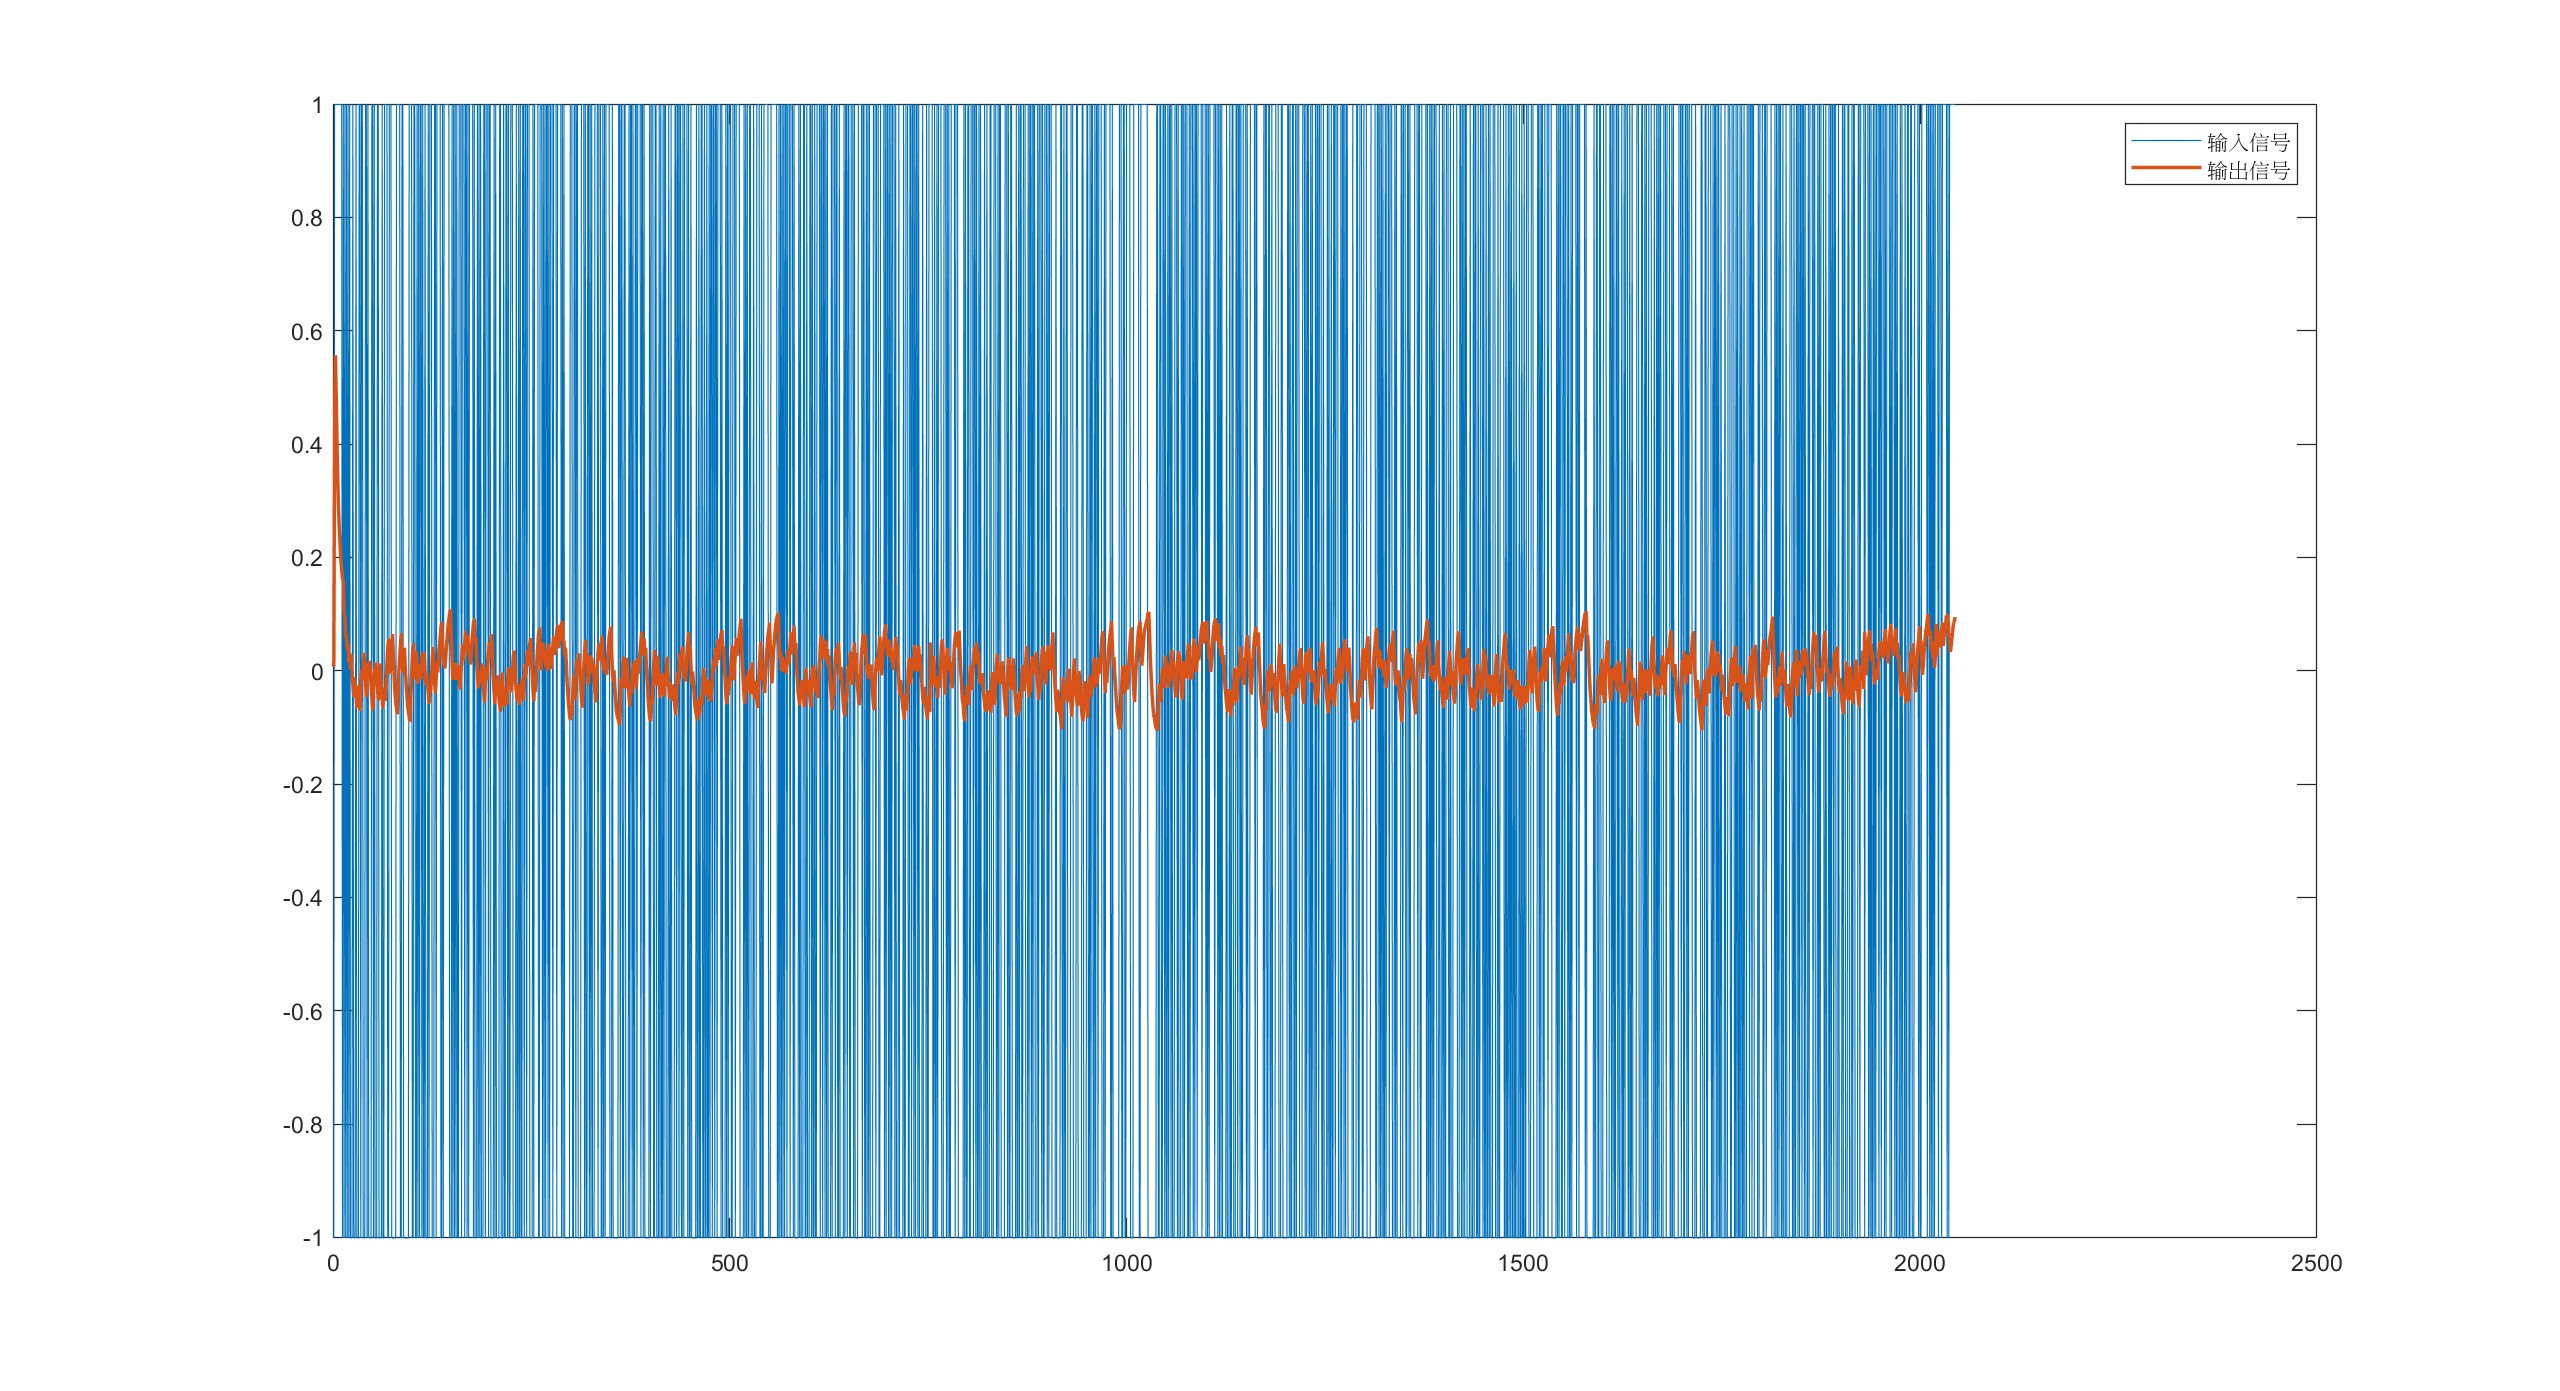
\includegraphics[width=\textwidth]
        {图片/D轴工作点0V输入输出曲线.jpg}
        \caption{D轴工作点0V输入输出曲线}
    \end{minipage}
    \begin{minipage}{0.5\textwidth}
        \centering
        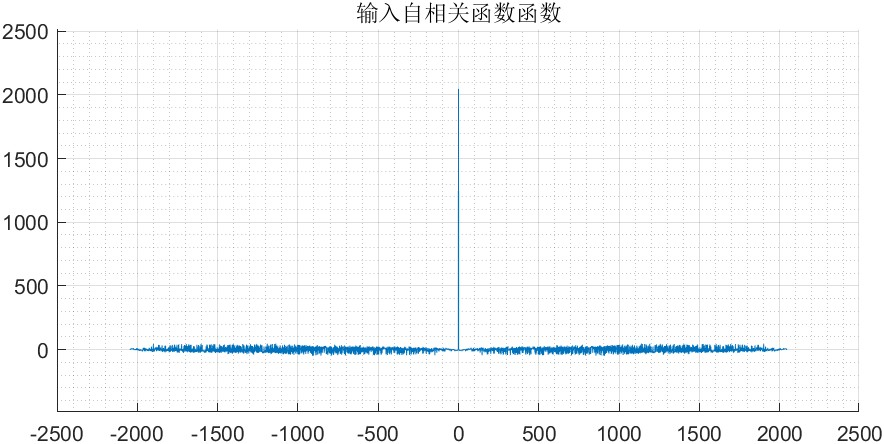
\includegraphics[width=\textwidth]
        {图片/D轴工作点0V输入自相关函数.jpg}
        \caption{D轴工作点0V输入自相关函数}    
    \end{minipage}
\end{figure}
\begin{figure}[H]
    \begin{minipage}{0.5\textwidth}
        \centering
        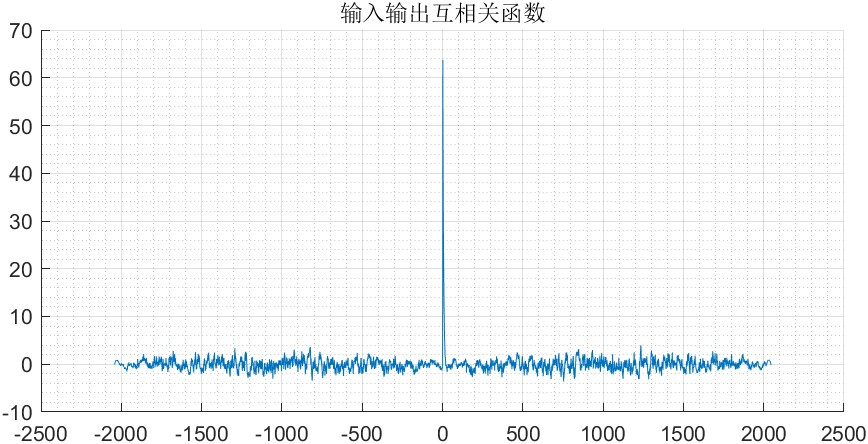
\includegraphics[width=\textwidth]
        {图片/D轴工作点0V输入输出互相关函数.jpg}
        \caption{D轴工作点0V输入输出互相关函数}
    \end{minipage}
    \begin{minipage}{0.5\textwidth}
        \centering
        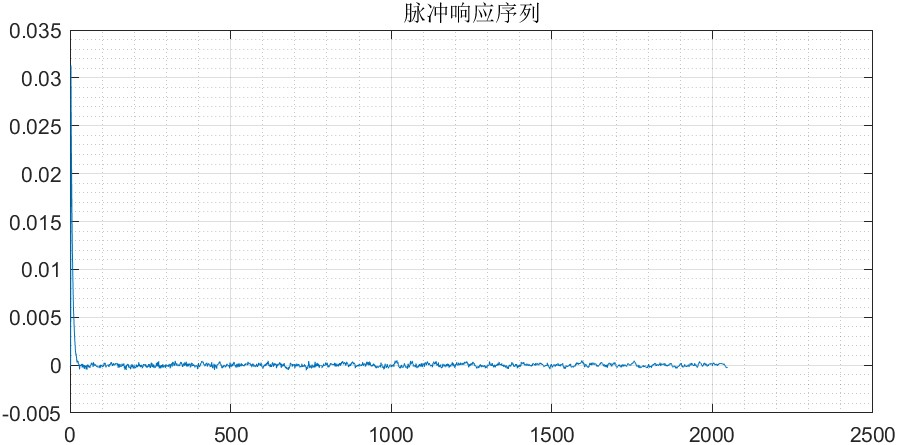
\includegraphics[width=\textwidth]
        {图片/D轴工作点0V脉冲响应序列.jpg}
        \caption{D轴工作点0V脉冲响应序列}
    \end{minipage}
\end{figure}

根据脉冲响应序列，其经过约16个采样周期后暂态响应结束，因此取Hankel矩阵阶次为8。
对Hankel矩阵进行归一化奇异值分解结果如下图所示。
\begin{figure}[H]
    \centering
    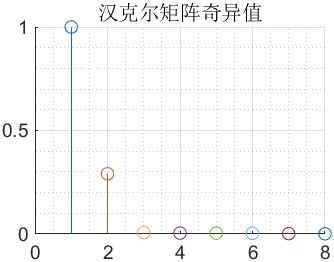
\includegraphics[width=0.8\textwidth]
    {图片/D轴工作点0V奇异值分解图.jpg}
    \caption{D轴工作点0V奇异值分解图}
\end{figure}

奇异值在第三个处发生跳变，因此取系统阶次为2，得到数值频域解和解析频域解如下图所示。
\begin{figure}[H]
    \centering
    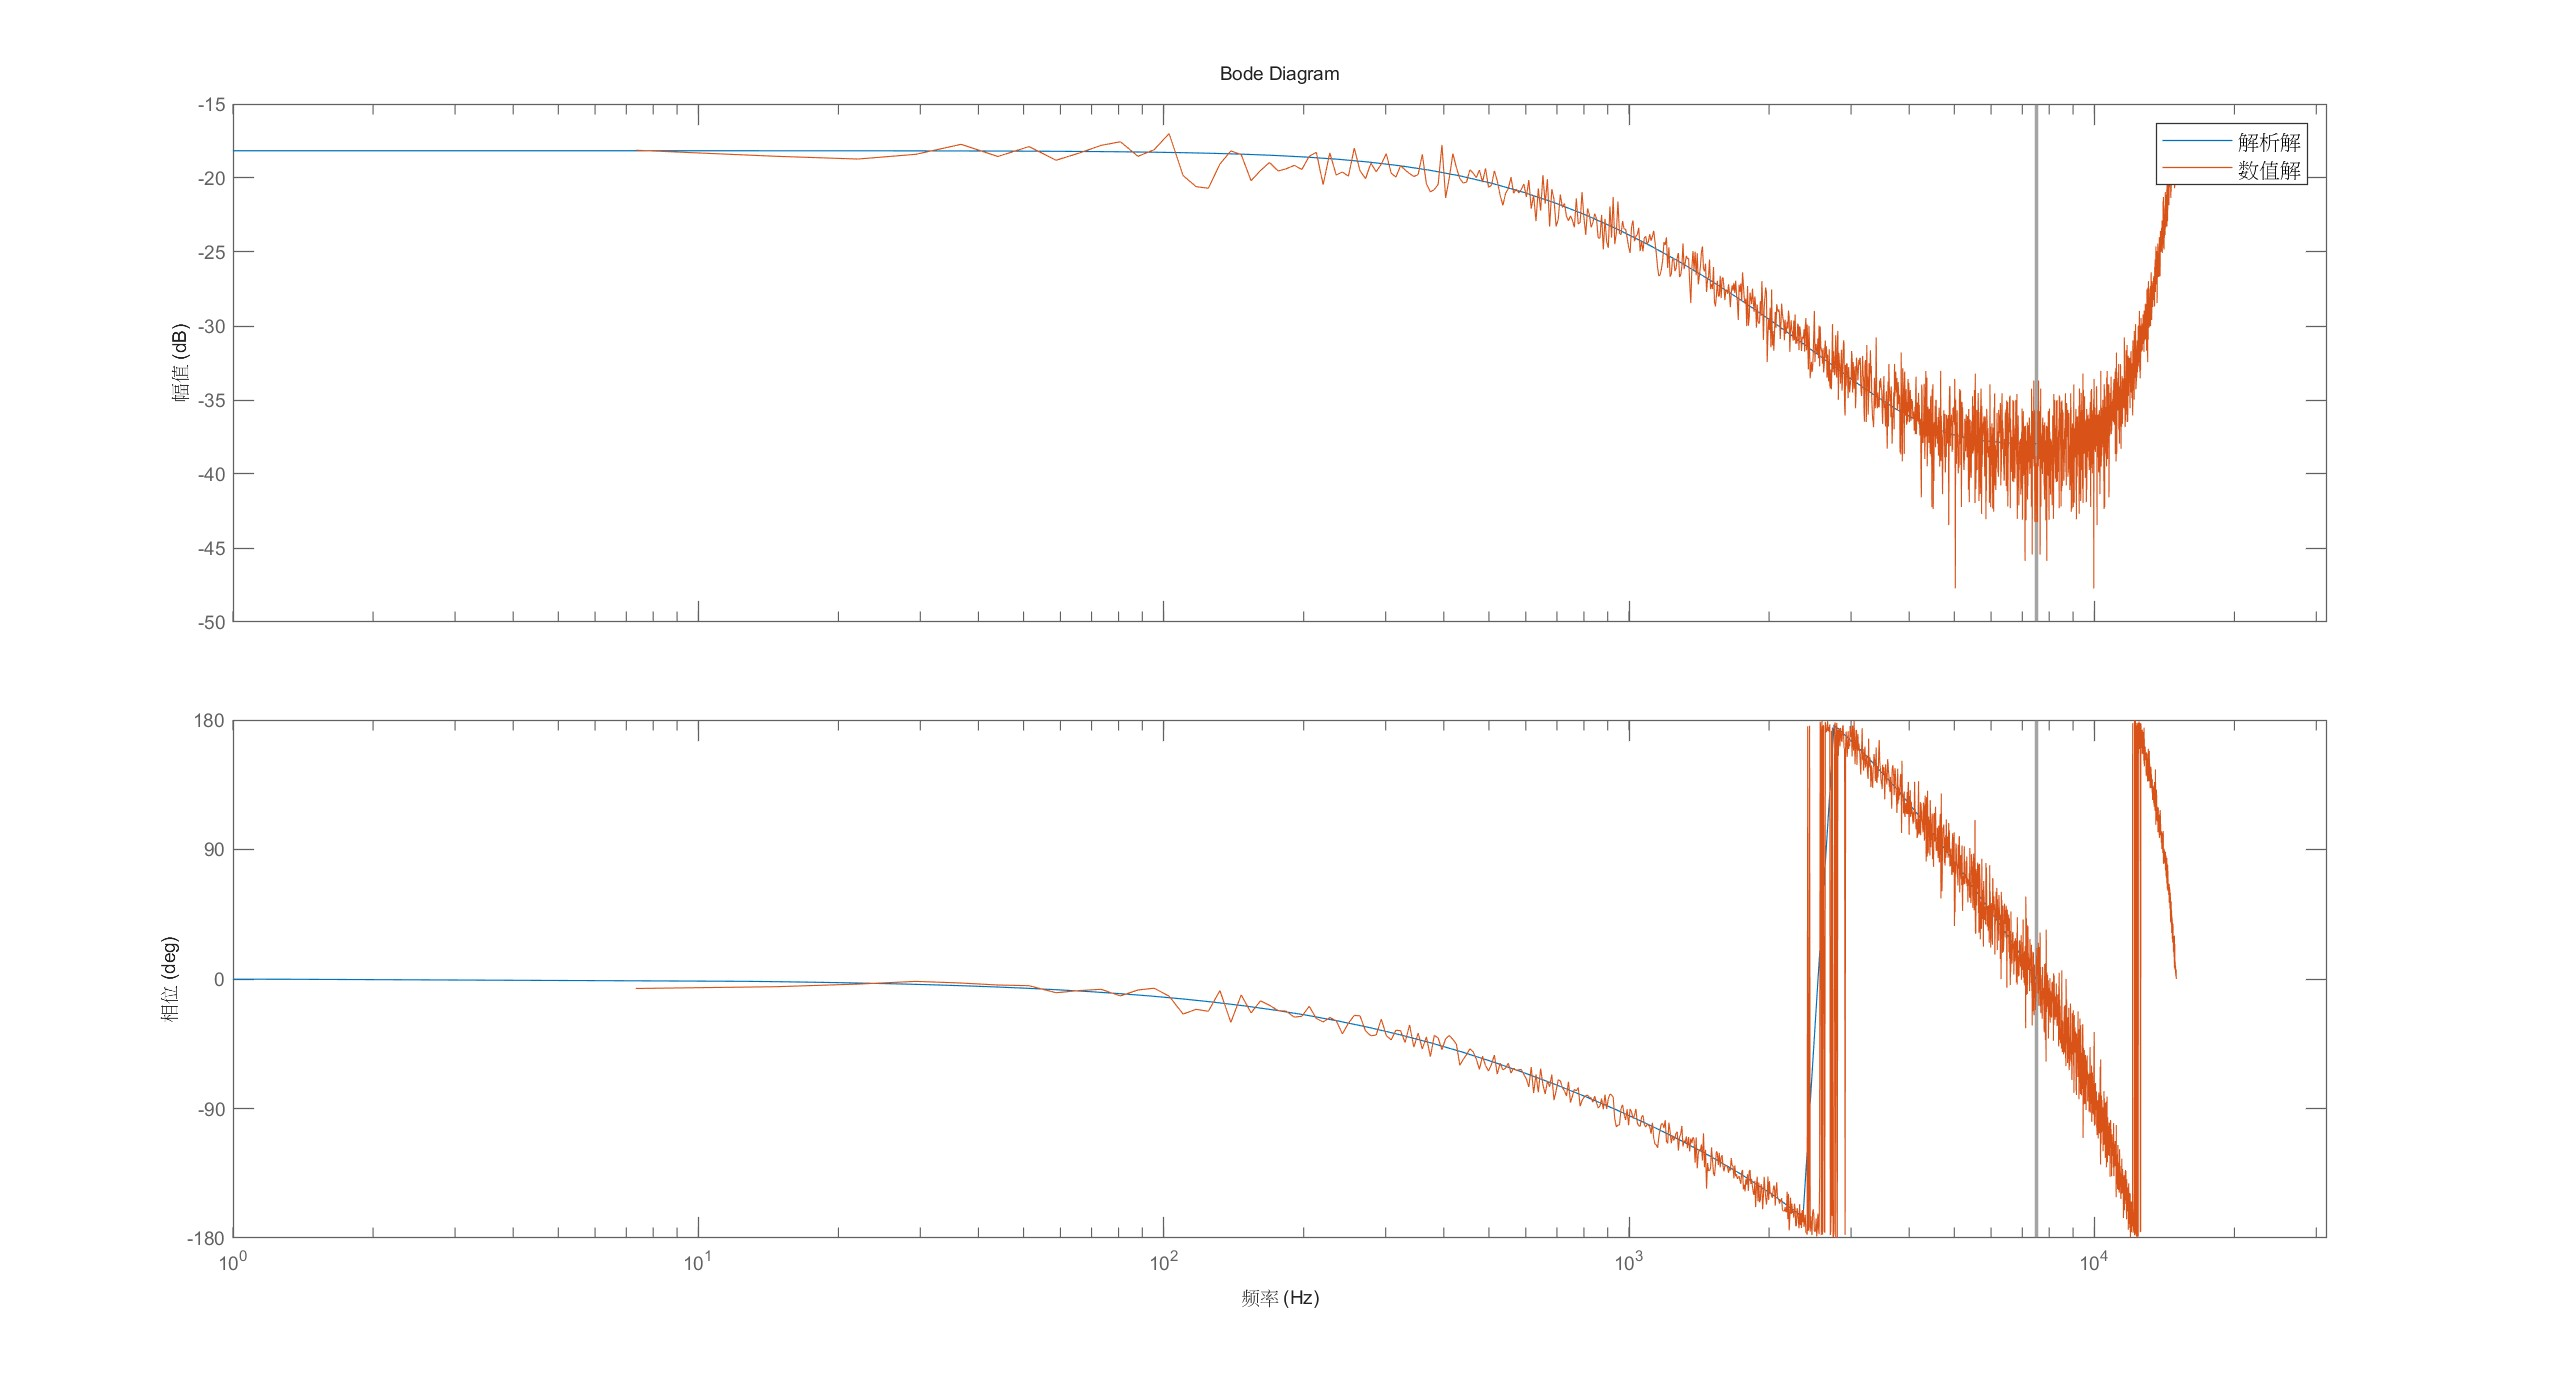
\includegraphics[width=0.8\textwidth]
    {图片/D轴工作点0V数值解和解析解对比.jpg}
    \caption{D轴工作点0V数值解和解析解对比}
\end{figure}

解析解与数值解幅频相关系数为98.89805\(\%\)，
相频相关系数为99.90722\(\%\)，拟合优度86.40194\(\%\)。整体处于较高水平。传递函数为
\(G(z)=\cfrac{-0.0001204  - 0.00006515 z^{-1} + 0.03132z^{-2}}{1 - 0.7754 z^{-1} - 0.03261z^{-2}}\)，两个极点为
0.8154和-0.04。从两个极点中分离出0.8154极点为PWM模态，而-0.04为D轴电路模态。
D轴同步电感可以计算为\(L_d=-\cfrac{R_sT_s}{\ln(z_p)}\)，
可得在0V工作点下D轴同步电感为\(L_d=1.86152\textrm{mH}\)。

后续工作点的辨识过程与上述类似，均采用Hankel矩阵阶次8，系统阶次2，选取幅值较大的极点为电路模态，
利用\(L_d=-\cfrac{R_sT_s}{\ln(z_p)}\)计算D轴电感，不再详述，仅列出较为重要的内容。

工作点2V时，得到的Hankel矩阵奇异值分解和频域响应对比如下图所示。
数值解与解析解的幅频相关系数为98.94669\(\%\)，
相频相关系数为99.94114\(\%\)，拟合优度87.09381\(\%\)。解析解传递函数为
\(G(z)=\cfrac{-0.0001405  + 0.0001453 z^{-1} + 0.03478z^{-2}}{1 - 0.765 z^{-1} - 0.03653z^{-2}}\)，两个极点为
0.8101和-0.0451。得到2V工作点下D轴同步电感为\(L_d=1.80467\textrm{mH}\)。
\begin{figure}[H]
    \begin{minipage}{0.5\textwidth}
        \centering
        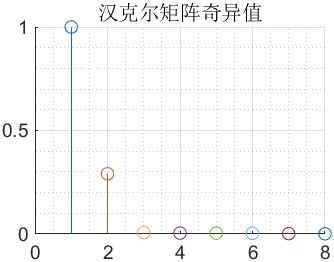
\includegraphics[width=\textwidth]
        {图片/D轴工作点2V奇异值分解图.jpg}
        \caption{D轴工作点2V奇异值分解图}
    \end{minipage}
    \begin{minipage}{0.5\textwidth}
        \centering
        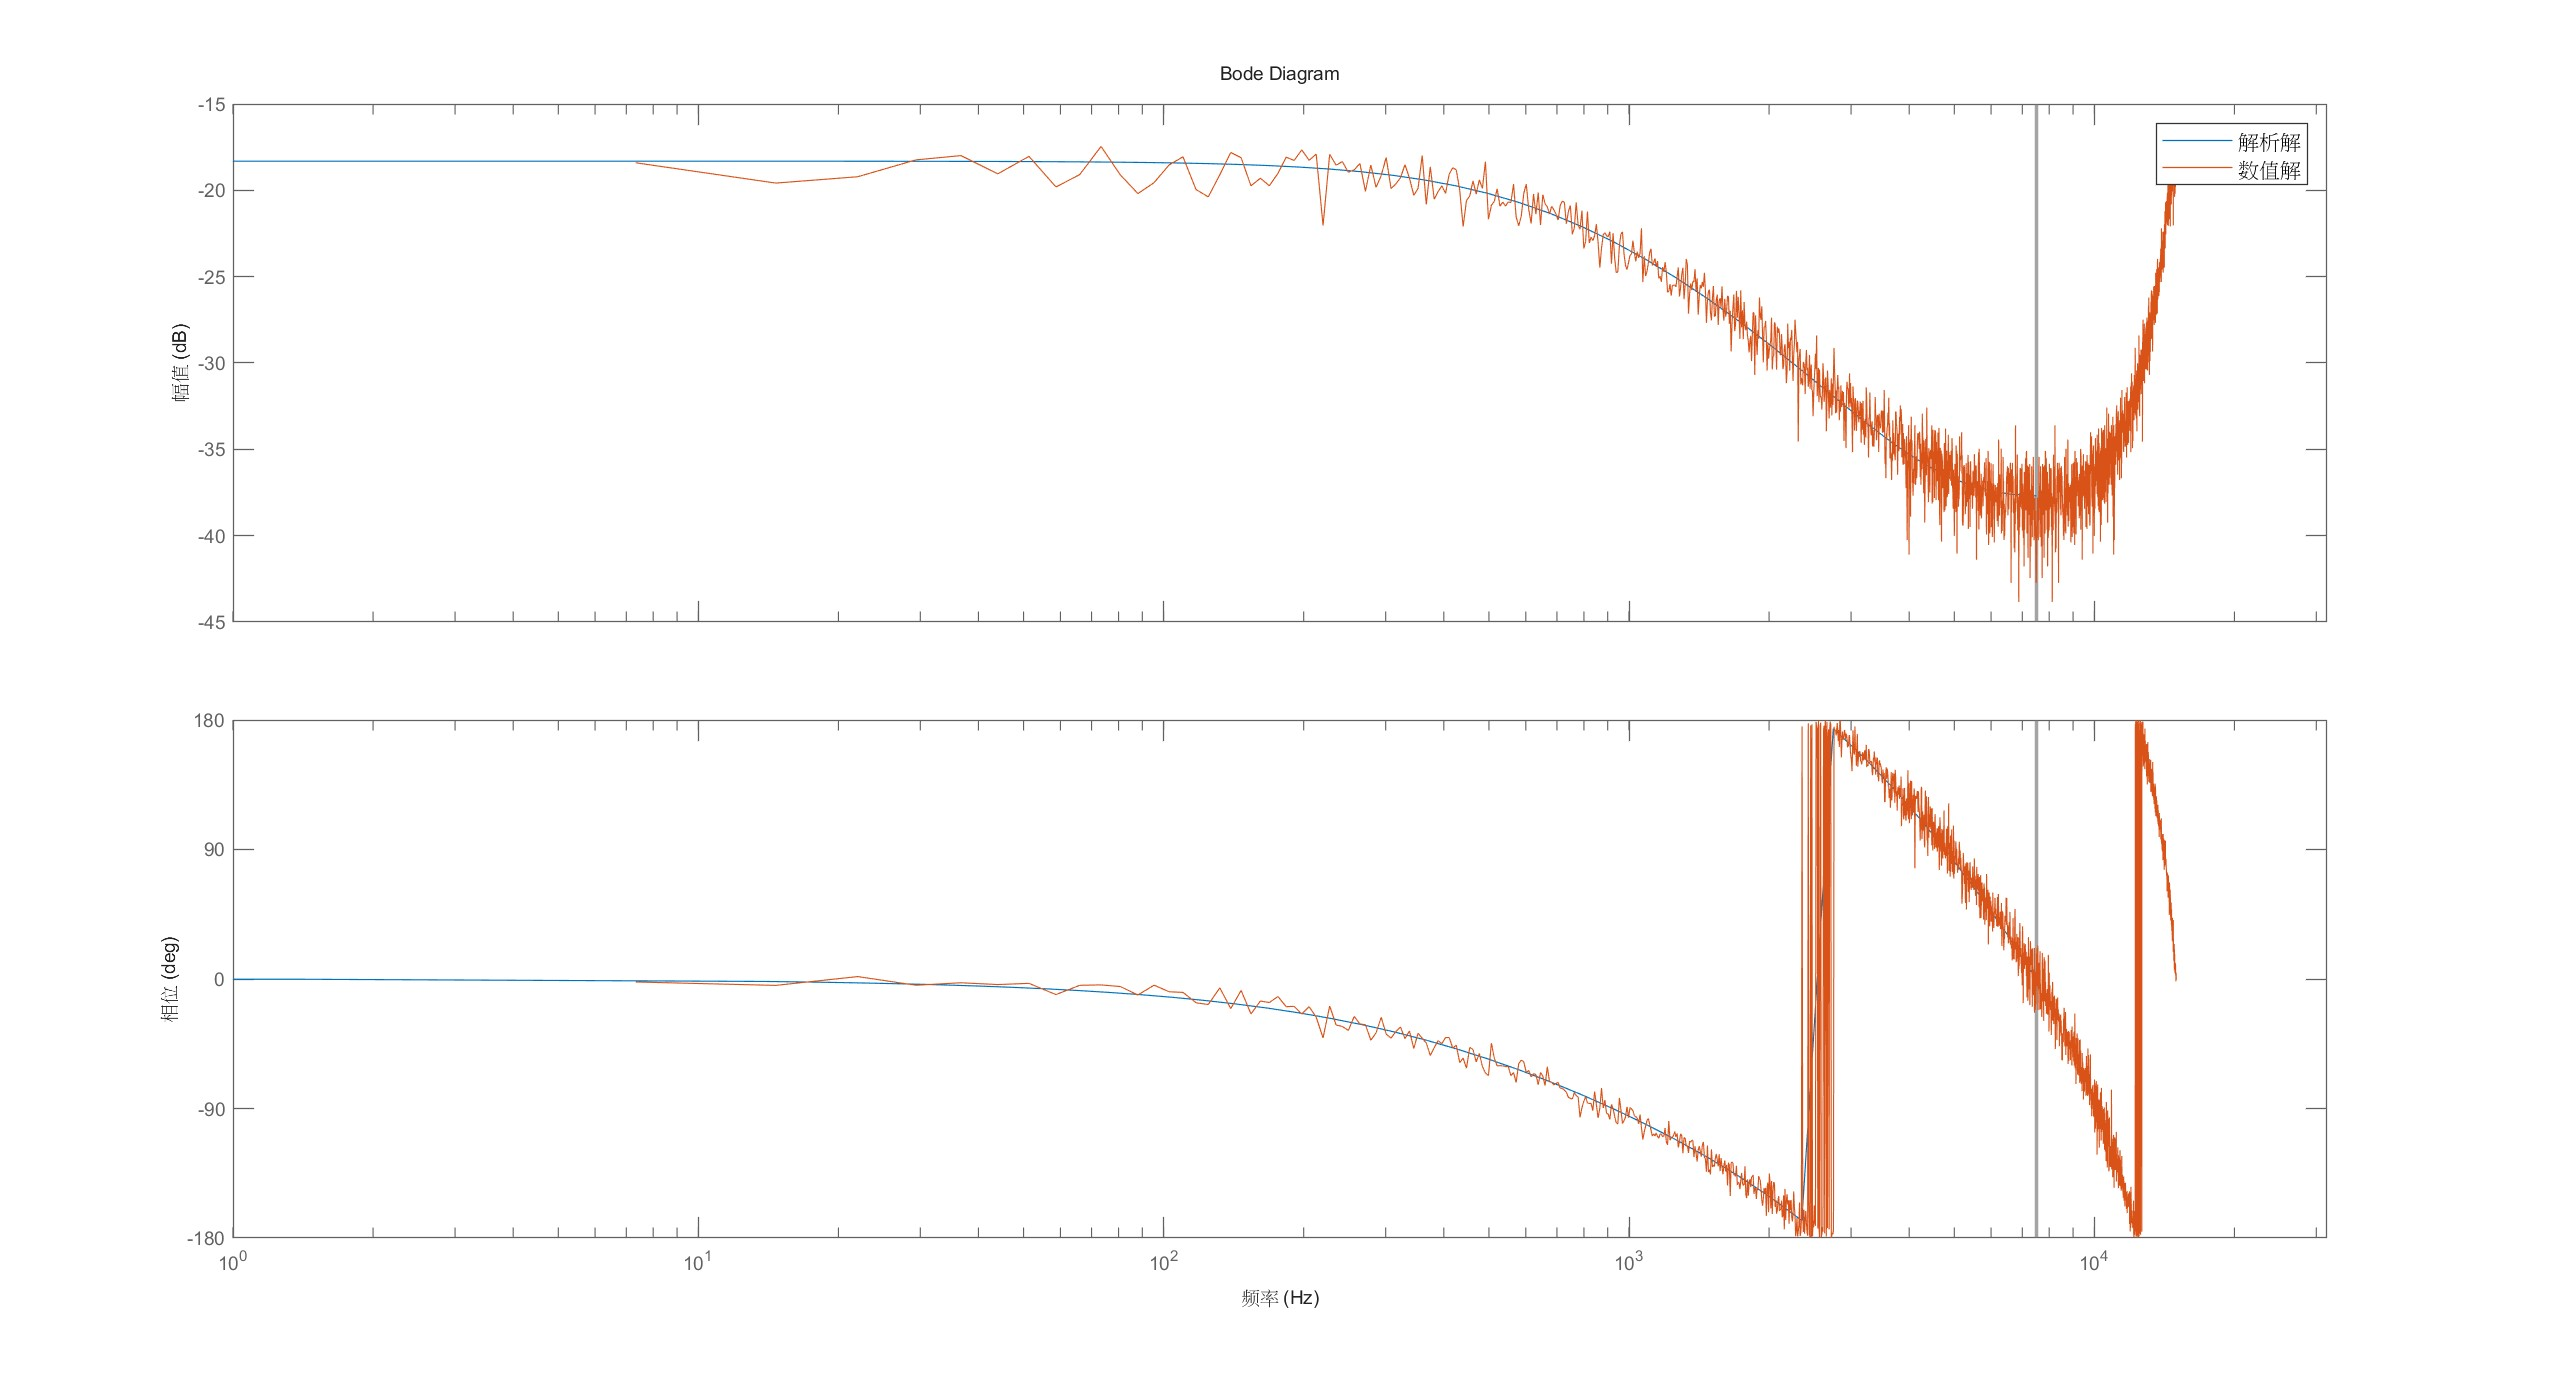
\includegraphics[width=\textwidth]
        {图片/D轴工作点2V数值解和解析解对比.jpg}
        \caption{D轴工作点2V数值解和解析解对比}
    \end{minipage}
\end{figure}

工作点4V时，得到的Hankel矩阵奇异值分解和频域响应对比如下图所示。
数值解与解析解的幅频相关系数为98.97066\(\%\)，
相频相关系数为99.91828\(\%\)，拟合优度86.93735\(\%\)。解析解传递函数为
\(G(z)=\cfrac{0.00005837  - 0.000171 z^{-1} + 0.034z^{-2}}{1 - 0.8461 z^{-1} + 0.0422z^{-2}}\)，两个极点为
0.7929和0.0532。得到4V工作点下D轴同步电感为\(L_d=1.63713\textrm{mH}\)。
\begin{figure}[H]
    \begin{minipage}{0.5\textwidth}
        \centering
        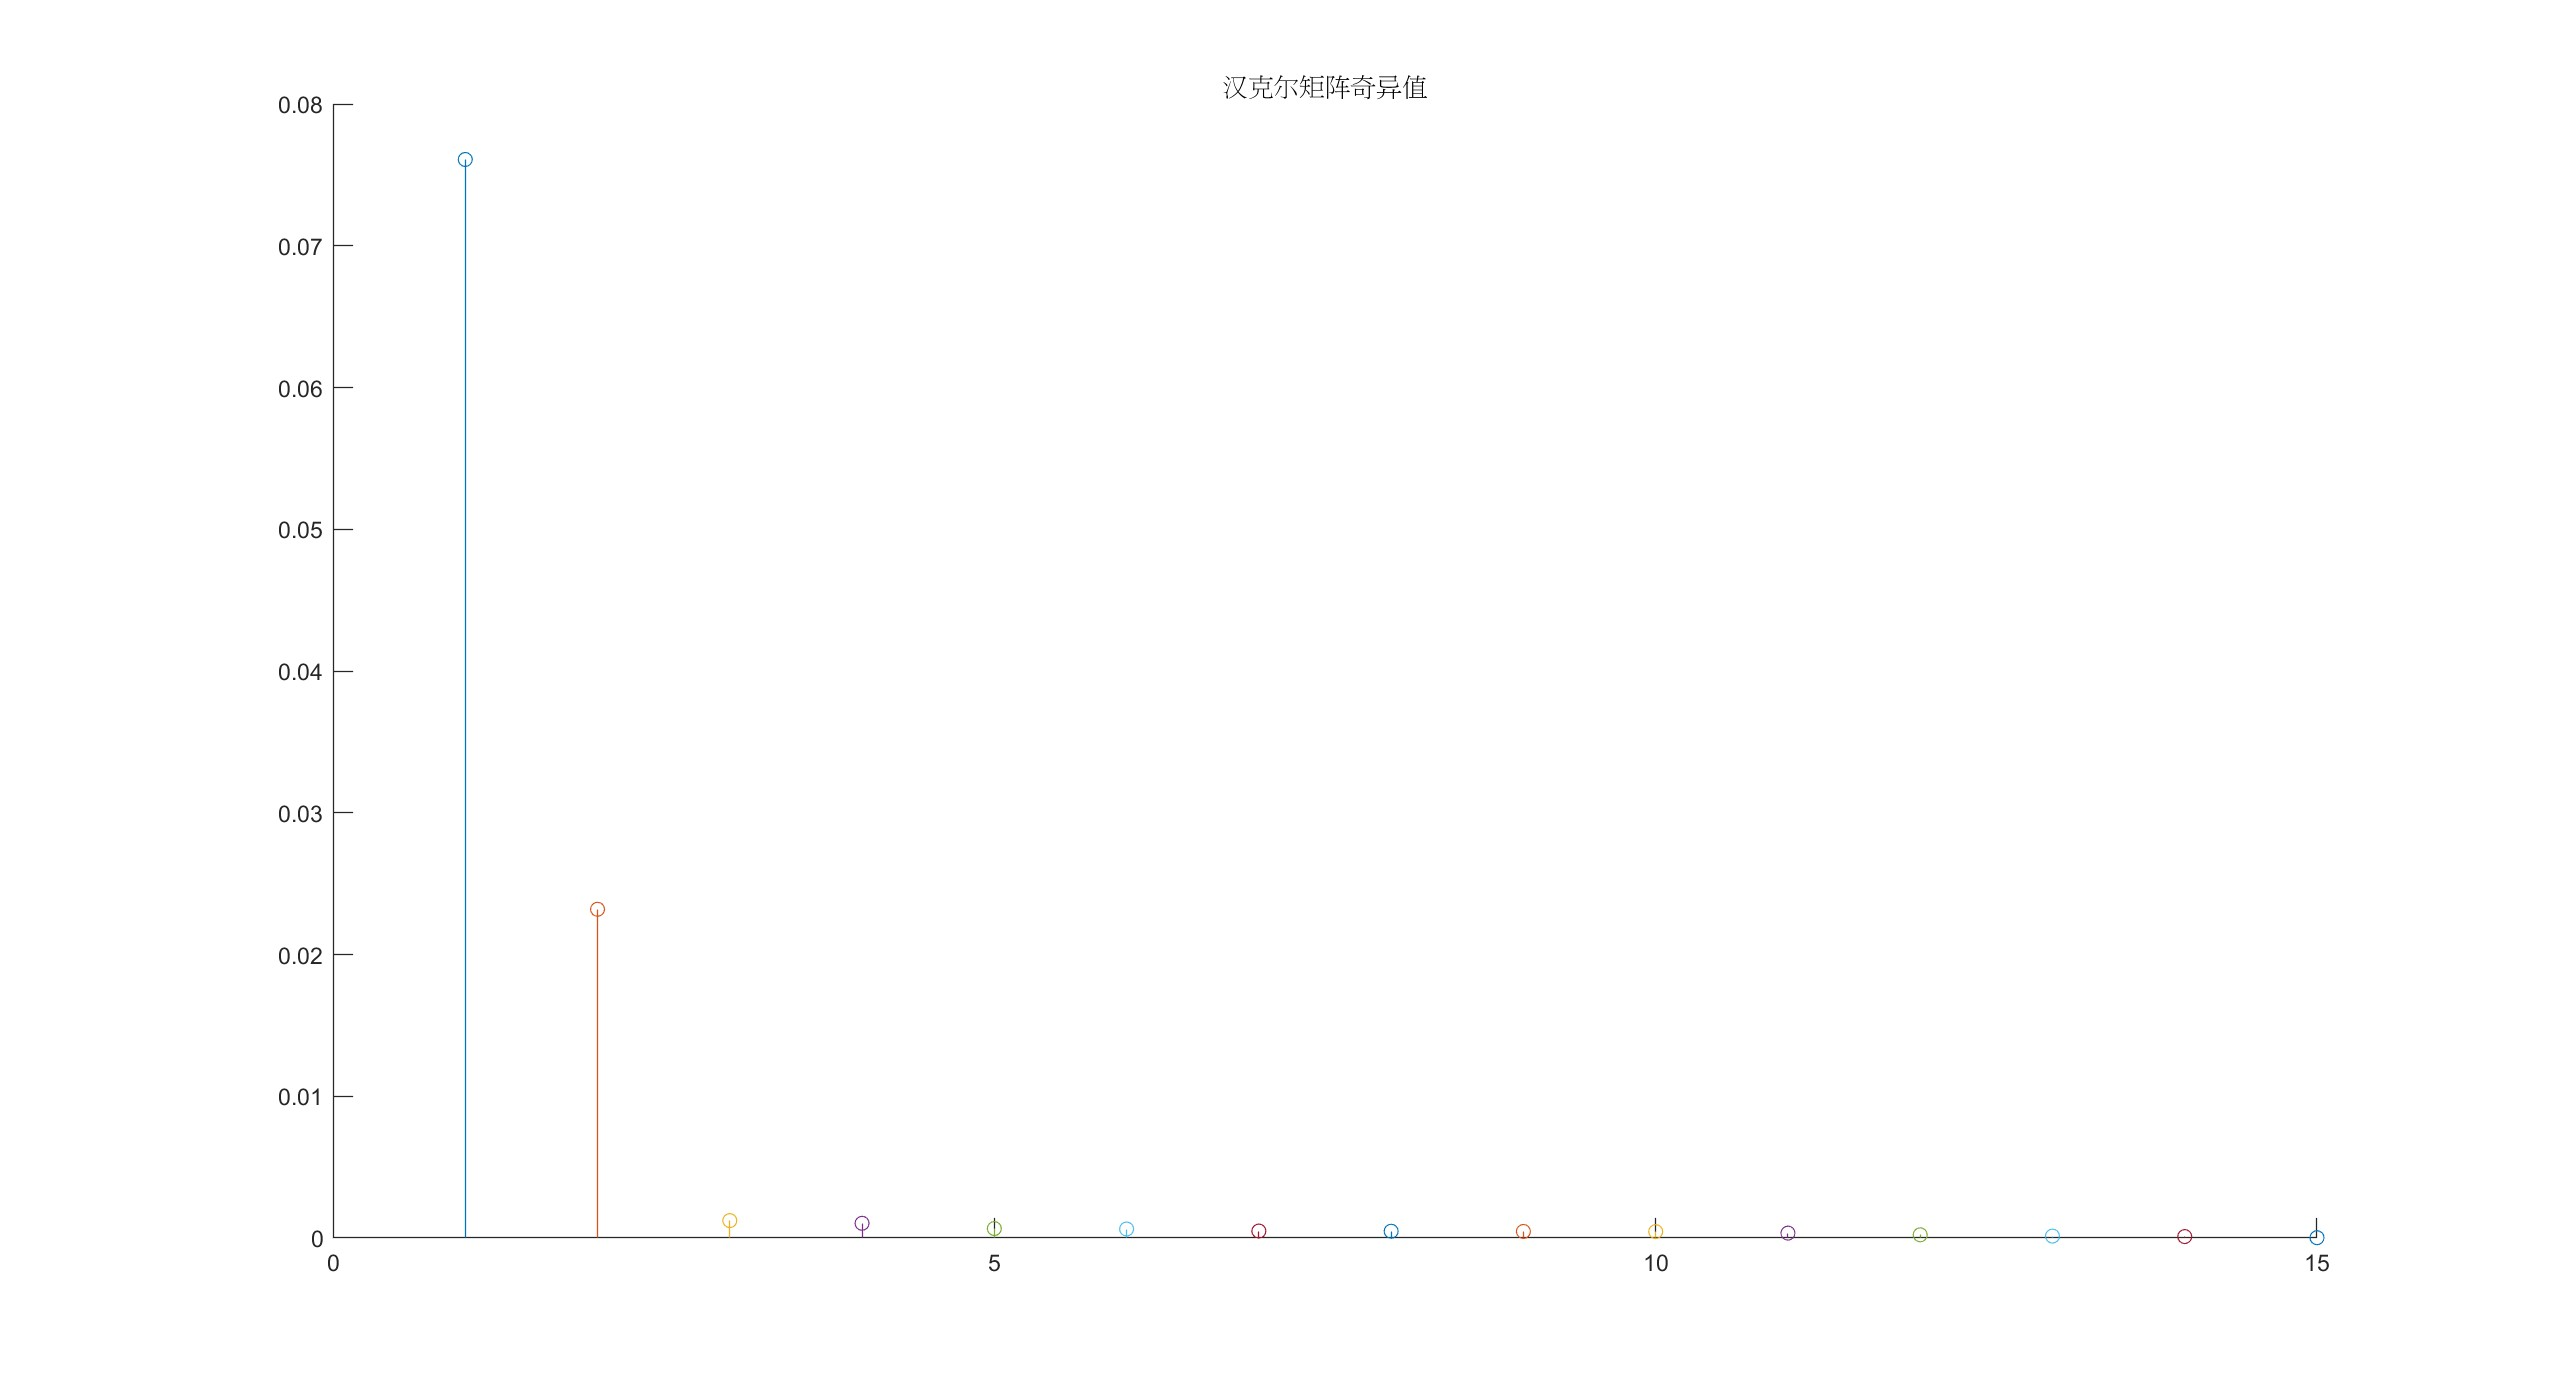
\includegraphics[width=\textwidth]
        {图片/D轴工作点4V奇异值分解图.jpg}
        \caption{D轴工作点4V奇异值分解图}
    \end{minipage}
    \begin{minipage}{0.5\textwidth}
        \centering
        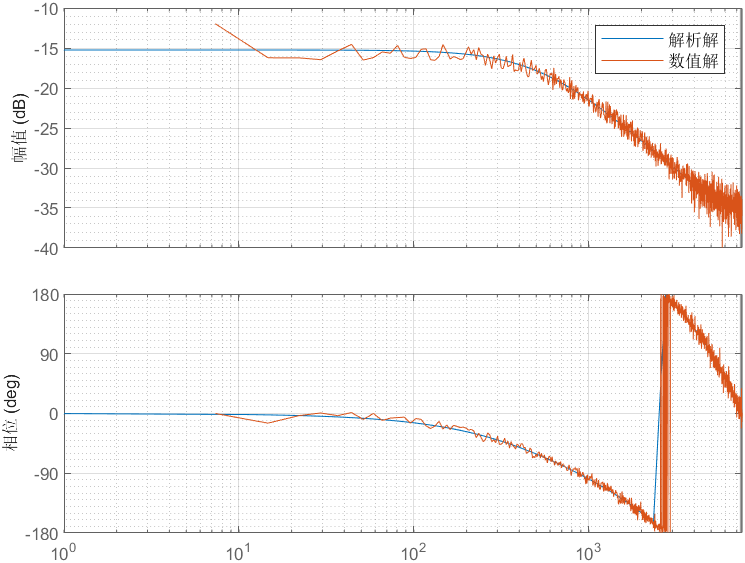
\includegraphics[width=\textwidth]
        {图片/D轴工作点4V数值解和解析解对比.jpg}
        \caption{D轴工作点4V数值解和解析解对比}
    \end{minipage}
\end{figure}

工作点-2V时，得到的Hankel矩阵奇异值分解和频域响应对比如下图所示。
数值解与解析解的幅频相关系数为98.88178\(\%\)，
相频相关系数为99.89867\(\%\)，拟合优度85.55227\(\%\)。解析解传递函数为
\(G(z)=\cfrac{0.00003966  + 0.00002372 z^{-1} + 0.0287z^{-2}}{1 - 0.7951 z^{-1} - 0.03771z^{-2}}\)，两个极点为
0.8400和-0.0499。得到-2V工作点下D轴同步电感为\(L_d=2.17947\textrm{mH}\)。
\begin{figure}[H]
    \begin{minipage}{0.5\textwidth}
        \centering
        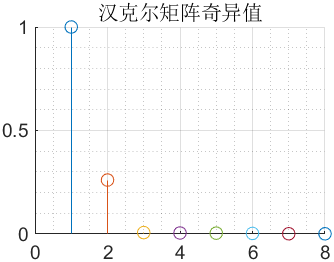
\includegraphics[width=\textwidth]
        {图片/D轴工作点-2V奇异值分解图.jpg}
        \caption{D轴工作点-2V奇异值分解图}
    \end{minipage}
    \begin{minipage}{0.5\textwidth}
        \centering
        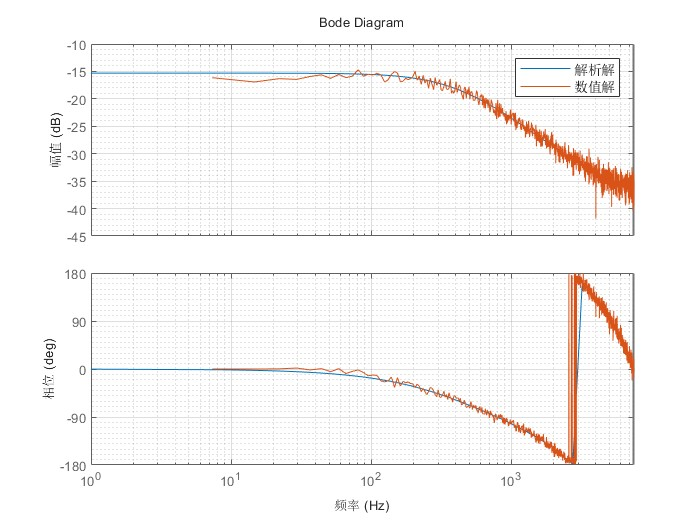
\includegraphics[width=\textwidth]
        {图片/D轴工作点-2V数值解和解析解对比.jpg}
        \caption{D轴工作点-2V数值解和解析解对比}
    \end{minipage}
\end{figure}

工作点-4V时，得到的Hankel矩阵奇异值分解和频域响应对比如下图所示。
数值解与解析解的幅频相关系数为98.73410\(\%\)，
相频相关系数为99.88621\(\%\)，拟合优度84.88066\(\%\)。解析解传递函数为
\(G(z)=\cfrac{0.00005562  - 0.0000877 z^{-1} + 0.02779z^{-2}}{1 - 0.7927 z^{-1} - 0.0462z^{-2}}\)，两个极点为
0.8472和-0.0545。得到-4V工作点下D轴同步电感为\(L_d=2.29122\textrm{mH}\)。
\begin{figure}[H]
    \begin{minipage}{0.5\textwidth}
        \centering
        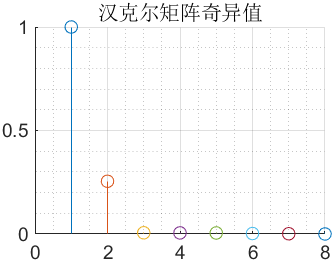
\includegraphics[width=\textwidth]
        {图片/D轴工作点-4V奇异值分解图.jpg}
        \caption{D轴工作点-4V奇异值分解图}
    \end{minipage}
    \begin{minipage}{0.5\textwidth}
        \centering
        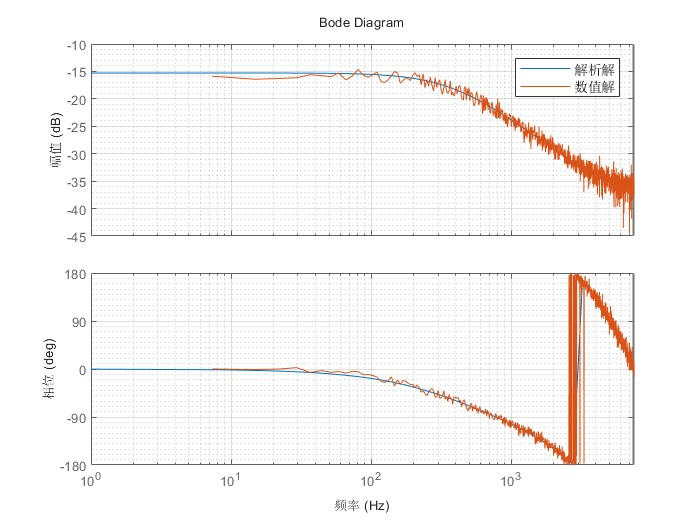
\includegraphics[width=\textwidth]
        {图片/D轴工作点-4V数值解和解析解对比.jpg}
        \caption{D轴工作点-4V数值解和解析解对比}
    \end{minipage}
\end{figure}

将上述五个工作点的D轴辨识结果汇总如下表所示。
\begin{table}[H]
    \centering
    \begin{tabular}{|c|c|c|c|c|}
        \hline
        工作点 & 幅频相关系数 & 相频相关系数 & 拟合优度 & \(L_d\)辨识值（mH）\\
        \hline
        \(U_d=-4\text{V}\)  & 98.73410\% & 99.88621\% & 84.88066\% & 2.29122\\
        \hline
        \(U_d=-2\text{V}\)  & 98.88178\% & 99.89867\% & 85.55227\% & 2.17947\\
        \hline
        \(U_d=0\text{V}\)   & 98.89805\% & 99.90722\% & 86.40194\% & 1.86152\\
        \hline
        \(U_d=2\text{V}\)   & 98.94669\% & 99.94114\% & 87.09381\% & 1.80467\\
        \hline
        \(U_d=4\text{V}\)   & 98.97066\% & 99.91828\% & 86.93735\% & 1.63713\\
        \hline
    \end{tabular}
    \caption{D轴各工作点HK辨识结果汇总}
    \label{tab:D轴各工作点辨识结果汇总}
\end{table}

根据HK伪随机辨识结果可以发现，随着工作点电压，也就是伪随机信号直流分量的增加，D轴同步电感辨识结果随之减小，
这与永磁同步电机的数学模型是匹配的，并非是算法问题，
接下来对此进行分析。

\subsubsection{工作点变化对D轴电感辨识结果的影响}

铁磁材料的磁化曲线如下图所示。可以发现，随着外界激发磁场强度H增大，磁感应强度B呈现出快速升高后逐渐饱和的现象，磁导率\(\mu=\cfrac{B}{H}\)
则呈现出先快速升高到极点后迅速下降的特点。磁导率的最大值称为铁磁材料的膝点，越过膝点就称为进入了磁饱和区，并且越过膝点越远，磁饱和程度越高。
\begin{figure}[H]
    \centering
    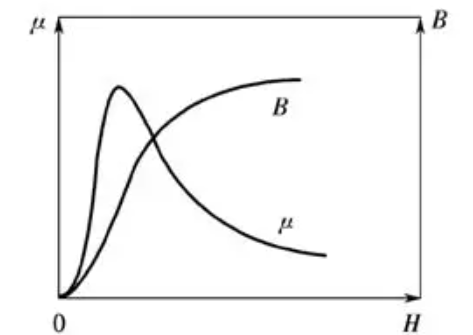
\includegraphics[width=0.4\textwidth]
    {图片/铁磁材料的磁化曲线.png}
    \caption{铁磁材料的磁化曲线}
\end{figure}

对于大部分永磁同步电机，转子磁场主要由永磁体提供，本身磁场强度较高，已进入磁饱和区。在D轴上，设永磁体磁动势为\(F_{c}\)为定值，
D轴电流产生的磁动势为\(F_{d}=Ni_d\)，其中\(N\)表示等效匝数。根据磁路欧姆定律，磁通量可以表示为：
\begin{equation*}
    \varPhi=\cfrac{F_{c}+F_{d}}{R_m}=\cfrac{F_{c}+Ni_d}{R_m}=\cfrac{\mu S(F_c+Ni_{d})}{l_c}
\end{equation*}

其中\(R_m\)为磁阻，表达式为\(R_m=\cfrac{l}{\mu S}\)，其中\(\mu\)表示磁导率，\(l\)表示磁路长度，\(S\)表示磁路横截面积。
磁阻主要分为三个部分：永磁体磁阻\(R_{pm}\)，气隙磁阻\(R_g\)，定子铁心磁阻\(R_{Fe}=\cfrac{l_{Fe}}{\mu_{Fe} S_{Fe}}\)。
其中永磁体磁阻和气隙磁阻可视为常数，和为\(R_c\)，定子铁心磁阻由于不同工作点的\(i_d\)不同而会发生变化。
因此将磁阻改写为\(R_m=R_{c}+\cfrac{l_{Fe}}{\mu S_{Fe}}\)。

HK辨识方法是在工作点附近的局部线性化结果，此时辨识得到的电感为增量电感，即\(L_d=\cfrac{\partial\psi}{\partial i_d}\)，其中
磁链为\(\psi=N\varPhi\)。由于等效匝数\(N\)不变，因此辨识电感为\(L_d=N\cfrac{d\varPhi}{di_d}\)。

代入磁路欧姆定律方程可得\(L_d=N\cfrac{d}{di_d}(\cfrac{F_e+Ni_d}{R_c+R_{Fe}})\)，分别求取微分可得
\(L_d=-N\cfrac{F_e}{R_c+R_{Fe}}\cfrac{dR_{Fe}}{di_d}+N^2\cfrac{(R_c+R_{Fe})-i_d\frac{dR_{Fe}}{di_d}}{(R_c+R_{Fe})^2}\)，整理得到：
\begin{equation*}
    L_d=\cfrac{N^2}{R_c+R_{Fe}}-\cfrac{N(F_e+Ni_d)}{(R_c+R_{Fe})^2}\cfrac{dR_{Fe}}{di_d}
\end{equation*}

当工作点电压升高，\(u_d>0\)时，电流工作点\(i_d>0\)，表现为助磁，加深磁场的饱和程度，使得磁导率\(\mu\)进一步下降，
定子铁心磁阻\(R_{Fe}=\cfrac{l_{Fe}}{\mu_{Fe} S_{Fe}}\)快速升高。这会带来两个结果：
第一，由于\(R_{Fe}\)迅速升高，使得\(\cfrac{N^2}{R_c+R_{Fe}}\)快速降低；第二，由于\(R_{Fe}\)呈现为上升趋势，因此
\(\cfrac{dR_{Fe}}{di_d}>0\)并且\(i_d\)升高，使得\(\cfrac{N(F_e+Ni_d)}{(R_c+R_{Fe})^2}\cfrac{dR_{Fe}}{di_d}\)项升高。
最终使得辨识得到的\(L_d\)呈现处随工作点电压升高而降低的现象。

而当工作电压降低，\(u_d<0\)时，电流工作点\(i_d<0\)，表现为去磁，减少磁场的饱和程度。在膝点之前磁导率\(\mu\)会随着\(u_d\)进一步的下降
而升高，也就能看到\(L_d\)随工作点电压降低而升高的现象。若\(i_d\)反向足够大，则会越过膝点，使得磁导率开始下降，\(L_d\)辨识结果降低。
但对于大部分永磁同步电机，若去磁电流过大，会使得永磁体产生不可逆的去磁，不利于电机工作，因此若进行磁场的弱磁或助磁控制，
需要谨慎选取给定电流，避免造成不可逆的永磁体损伤。

再次在多个工作点进行辨识，可以绘制得到D轴同步电感随工作点电压变化的关系图如下所示。考虑到噪声干扰和辨识偏差，据图可以认为，
上述定性推导是正确的，D轴同步电感辨识结果随工作点电压升高而降低为物理系统规律，并非算法误差。
\begin{figure}[H]
    \centering
    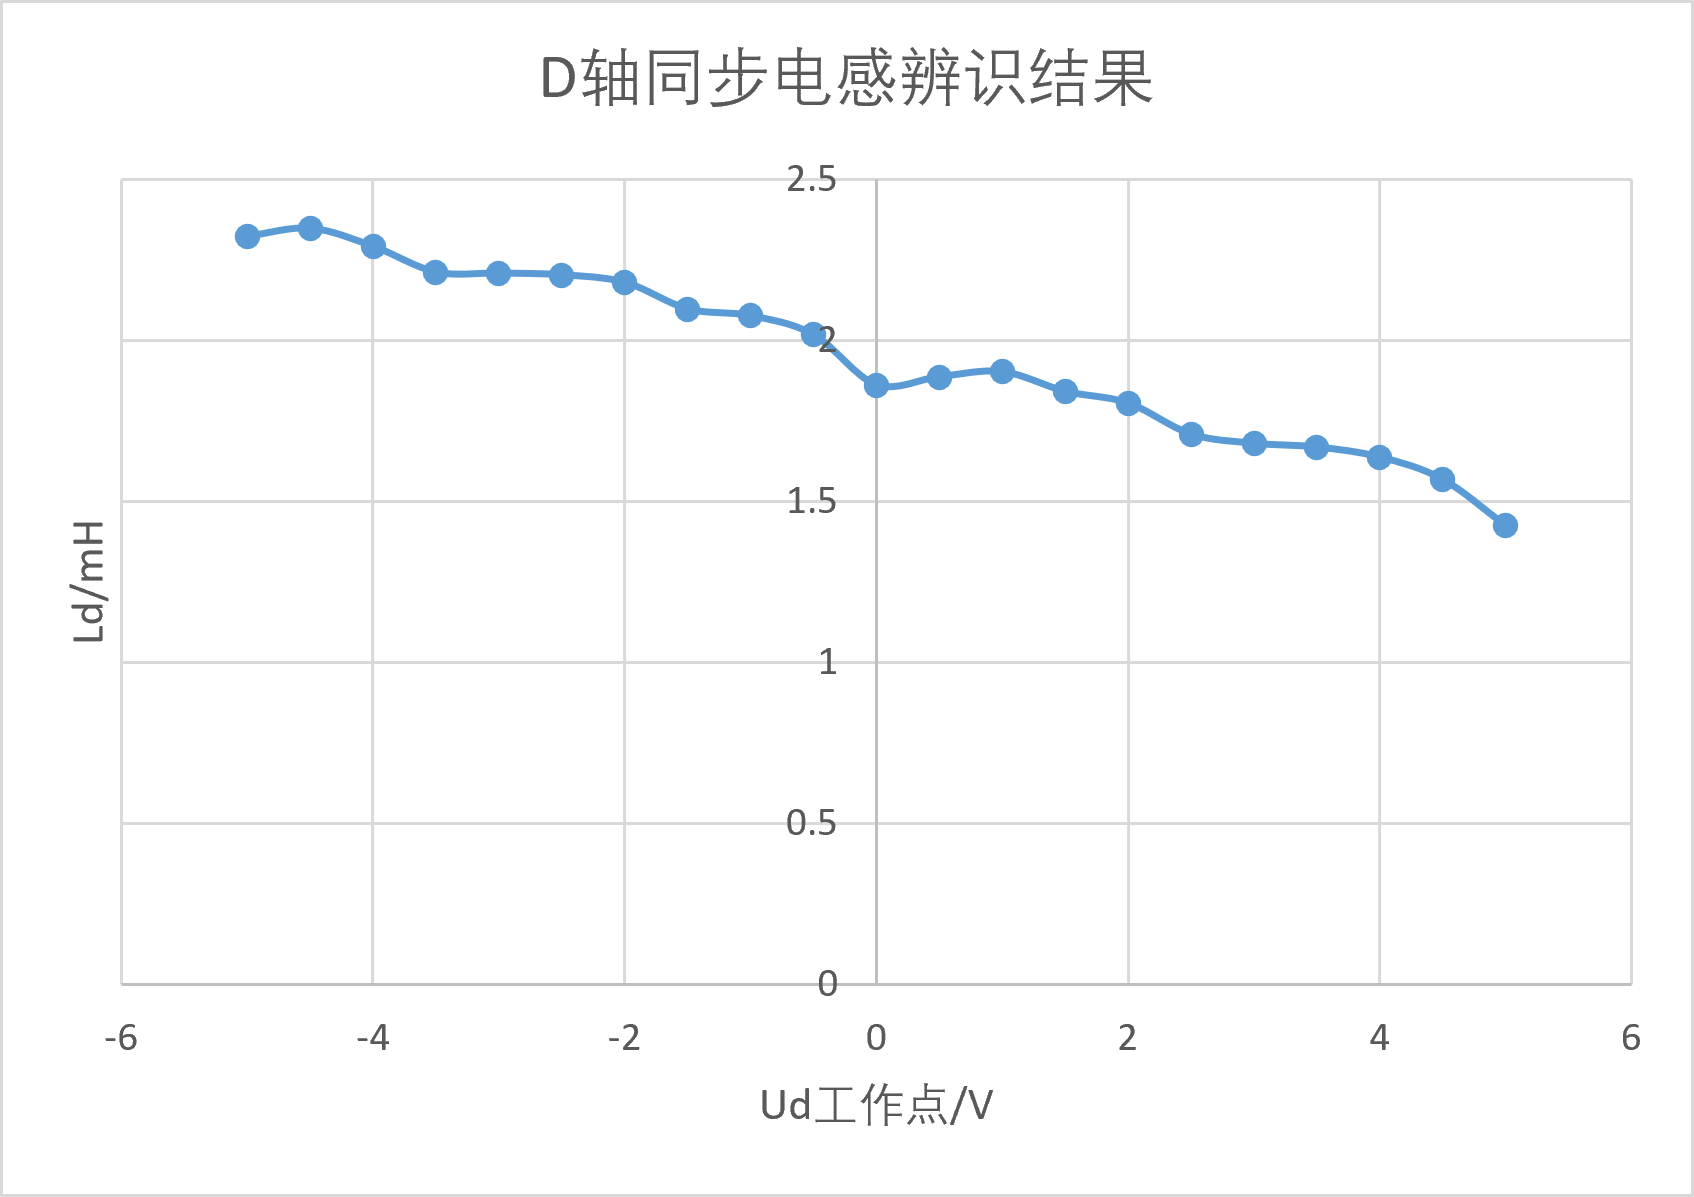
\includegraphics[width=0.8\textwidth]
    {图片/D轴同步电感辨识曲线.png}
    \caption{D轴同步电感辨识曲线}
\end{figure}

考虑到在大部分FOC控制中选取\(i_d=0\)作为工作点，因此取\(u_d=0\)时的辨识结果为如下，
满足相间电感估计得到的同步电感范围\(L_d\in(1.76917,1.94354)\textrm{mH}\)。
\begin{equation*}
    L_{dO}=1.86152\textrm{mH}
\end{equation*}

\subsection{永磁体磁链测量\label{sec:永磁体磁链测量}}

基于相电阻\(R_s\)和D轴同步电感\(L_d\)的辨识结果，可以在稳态情况下实现对永磁体磁链\(\psi_m\)的辨识。

对于电路方程\eqref{eq:同步坐标系下电路方程}，只考虑Q轴情况下可以改写为：
\begin{equation*}
    u_q=R_si_q+L_q\cfrac{di_q}{dt}+\omega_e(L_di_d+\psi_m)
\end{equation*}

进行\(u_q\)给定的开环拖动，在稳态情况下\(i_q\)不再变化，因此\(\cfrac{di_q}{dt}=0\)，可以将Q轴电路方程改写为
\(u_q=R_si_q+\omega_e(L_di_d+\psi_m)\)，可以变形为：
\begin{equation*}
    \psi_m=\cfrac{u_q-R_si_q}{\omega_e}-L_di_d
\end{equation*}

其中\(u_q\)为给定量，\(R_s,L_d\)通过上述两节完成了辨识，可以视为定值，\(i_d,i_q,\omega_e\)均可以进行测量。
按照上式实时计算永磁体磁链并回传到上位机，期间调整\(u_q\)以验证各个工作点下工作的一致性，波形如下图所示。
\begin{figure}[H]
    \centering
    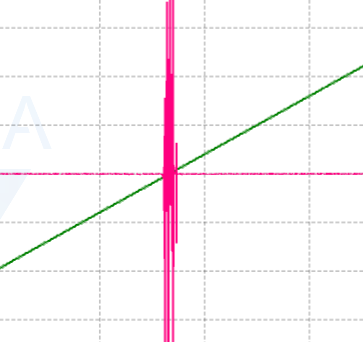
\includegraphics[width=0.8\textwidth]
    {图片/永磁体磁链辨识波形.png}
    \caption{永磁体磁链辨识波形（绿：\(u_q\)，红：\(\psi_m\)）}
\end{figure}

可以发现，当\(u_q\)给定较小时，辨识得到的\(\psi_m\)变化剧烈，这主要是因为\(u_q\)较小时转速较慢，
\(\omega_e\)较小，使得测量误差和噪声被由于分母太小而被放大。随着\(u_q\)给定值提高，电机转速升高，信噪比会逐步提高，
对永磁体磁链的辨识结果逐渐收敛到特定值。
取\(2<|u_q|<5.5\)，以0.1V为单位绘制\(\psi_m\)随\(u_q\)变化的关系图如下所示。
\begin{figure}[H]
    \centering
    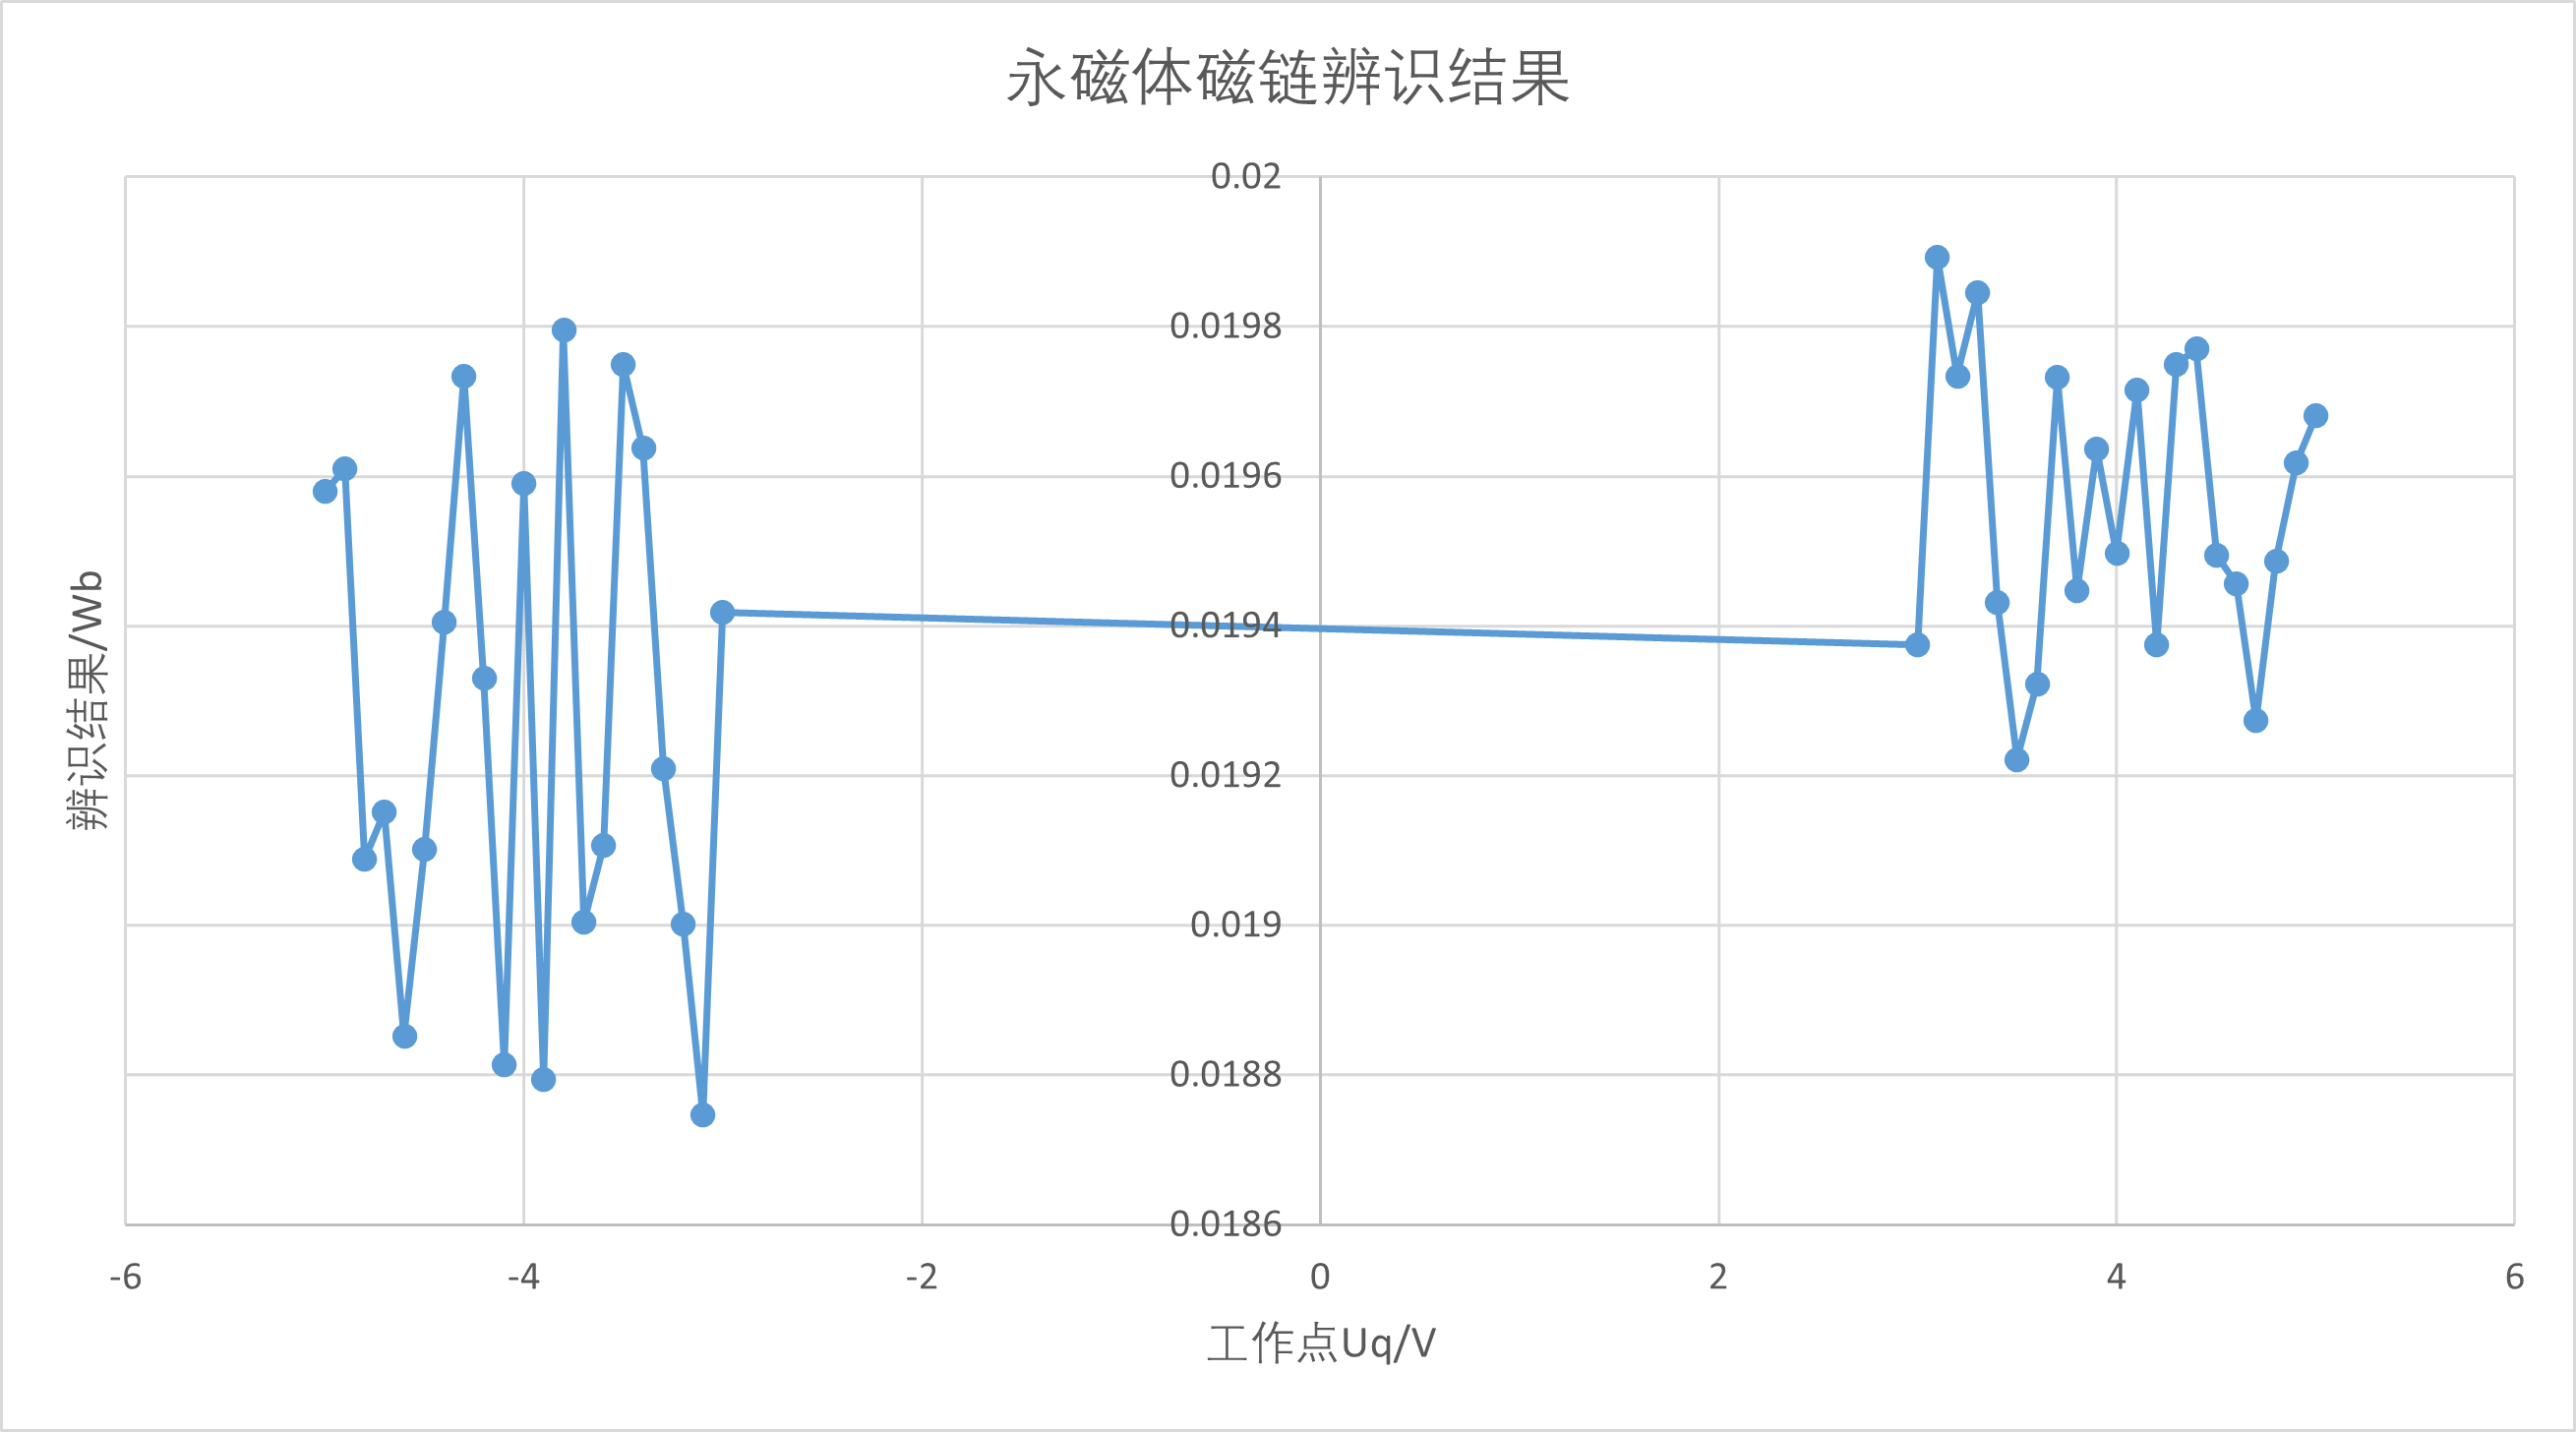
\includegraphics[width=0.8\textwidth]
    {图片/永磁体磁链辨识结果.png}
    \caption{永磁体磁链辨识结果}
\end{figure}

计算得到平均值为9.65548mWb，标准差0.000172651，相对标准误差为1.79\(\%\)，数据的精准度较高，可以近似认为在各个工作点附近永磁体磁链
不变，符合物理规律。

因此永磁体磁链辨识结果为：
\begin{equation*}
    \psi_{mO}=9.65548\textrm{mWb}
\end{equation*}

\subsection{Q轴同步电感辨识}
最后进行Q轴同步电感的辨识。根据电路方程有：
\begin{equation*}
    u_q=R_si_q+L_q\cfrac{di_q}{dt}+\omega_e(L_di_d+\psi_m)
\end{equation*}

理想情况下，若能保持严格锁定转轴，则\(\omega_e=0\)，Q轴可以退化为与进行D轴电感辨识时类似的一阶RL电路。但由于电磁转矩
\(T_e=\cfrac32pi_qi_d(L_d-L_q)+\cfrac32\psi_mpi_q\propto i_q\)
，一旦\(i_q\)产生响应就会差生电磁转矩。并且在高频变化的伪随机\(u_q\)
作用下，会产生高频变化的\(i_q\)，电磁转矩也随之发生变化，这对锁轴的提出了很高要求。

此外，由于电机磁路不对称有\(L_q\ge L_d\)，这点从式\eqref{eq:同步电感定义式}可以看出，
主要是因为D轴定义为与永磁体磁链平行的方向，磁饱和程度较高。
而时间常数\(\tau=\cfrac LR\)，因此Q轴时间常数一般会比D轴更大，脉冲响应需要更长时间
达到稳态，因此可以适当增大Hankel矩阵阶次到15。而系统阶次，考虑到理想情况下PWM模态的贡献，选取为2。
此外由于DQ轴的磁路不对称，Q轴由于反电动势存在和较大的同步电感存在，使得Q轴的电流响应幅度小于D轴，
为了获取较高的信噪比，需要增大激励电压的幅值，因此选取伪随机参数为幅值2，工作点0。

\subsubsection{电气锁轴方法\label{sec:电气锁轴方法}}
首先尝试进行电气锁轴，其主要原理是通过\(i_d\)的电流闭环，产生一个方向恒定的磁场吸引转子与之对齐，并且通过将\(i_d\)闭环到
较高水平确保能够较为牢固的吸住转子，在此基础上进行Q轴的伪随机辨识。下图是D轴电流闭环\(i_d=0.5A\)的HK辨识结果。
\begin{figure}[H]
    \centering
    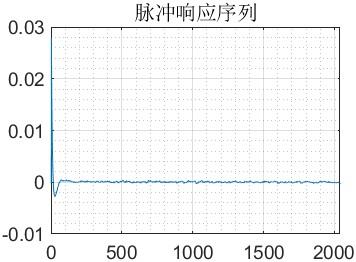
\includegraphics[width=0.8\textwidth]
    {图片/电气锁轴脉冲响应序列.jpg}
    \caption{电气锁轴脉冲响应序列}
\end{figure}

根据脉冲响应序列可以发现脉冲响应存在震荡，说明原系统存在欠阻尼的一对共轭极点。
进行奇异值分解和传递函数辨识结果如下所示。
\begin{figure}[H]
    \begin{minipage}{0.5\textwidth}
        \centering
        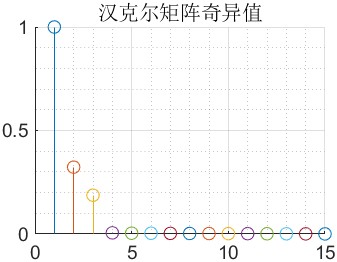
\includegraphics[width=\textwidth]
        {图片/电气锁轴奇异值分解图.jpg}
        \caption{电气锁轴奇异值分解图}
    \end{minipage}
    \begin{minipage}{0.5\textwidth}
        \centering
        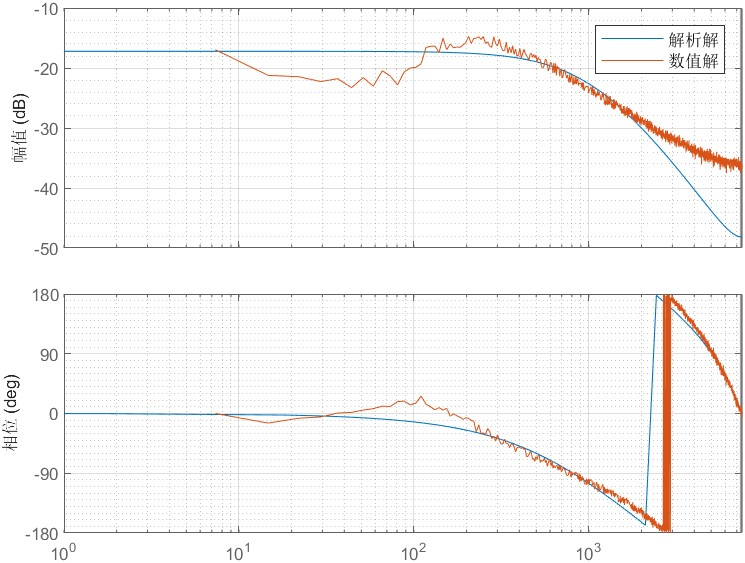
\includegraphics[width=\textwidth]
        {图片/电气锁轴数值解与解析解对比.jpg}
        \caption{电气锁轴数值解与解析解对比}
    \end{minipage}
\end{figure}

可以发现，电气锁轴不采用机械锁轴，难以确保转子锁定。而转子一旦开始转动，则PWM自身模态、Q轴RL电路模态、转动耦合模态
（主要由\(\omega_e(L_di_d+\psi_m)\)引起）等相互作用，
污染了辨识结果，使得难以从传递函数中提取出所需的信息。

\subsubsection{机械堵转方法\label{sec:机械堵转方法}}
接下来尝试机械堵转，辨识结果如下。
\begin{figure}[H]
    \centering
    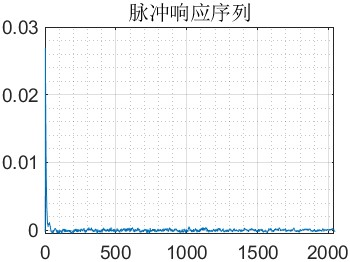
\includegraphics[width=0.8\textwidth]
    {图片/机械堵转脉冲响应序列.jpg}
    \caption{机械堵转脉冲响应序列}
\end{figure}

可以发现，通过机械堵转可以大幅降低脉冲响应中的震荡，使得辨识转动耦合模态含量降低。但由于无法严格锁轴，存在微动，因此无法完全杜绝
转动耦合模态带来的震荡。

对机械堵转进行奇异值分解和传递函数辨识，结果如下图所示
\begin{figure}[H]
    \begin{minipage}{0.5\textwidth}
        \centering
        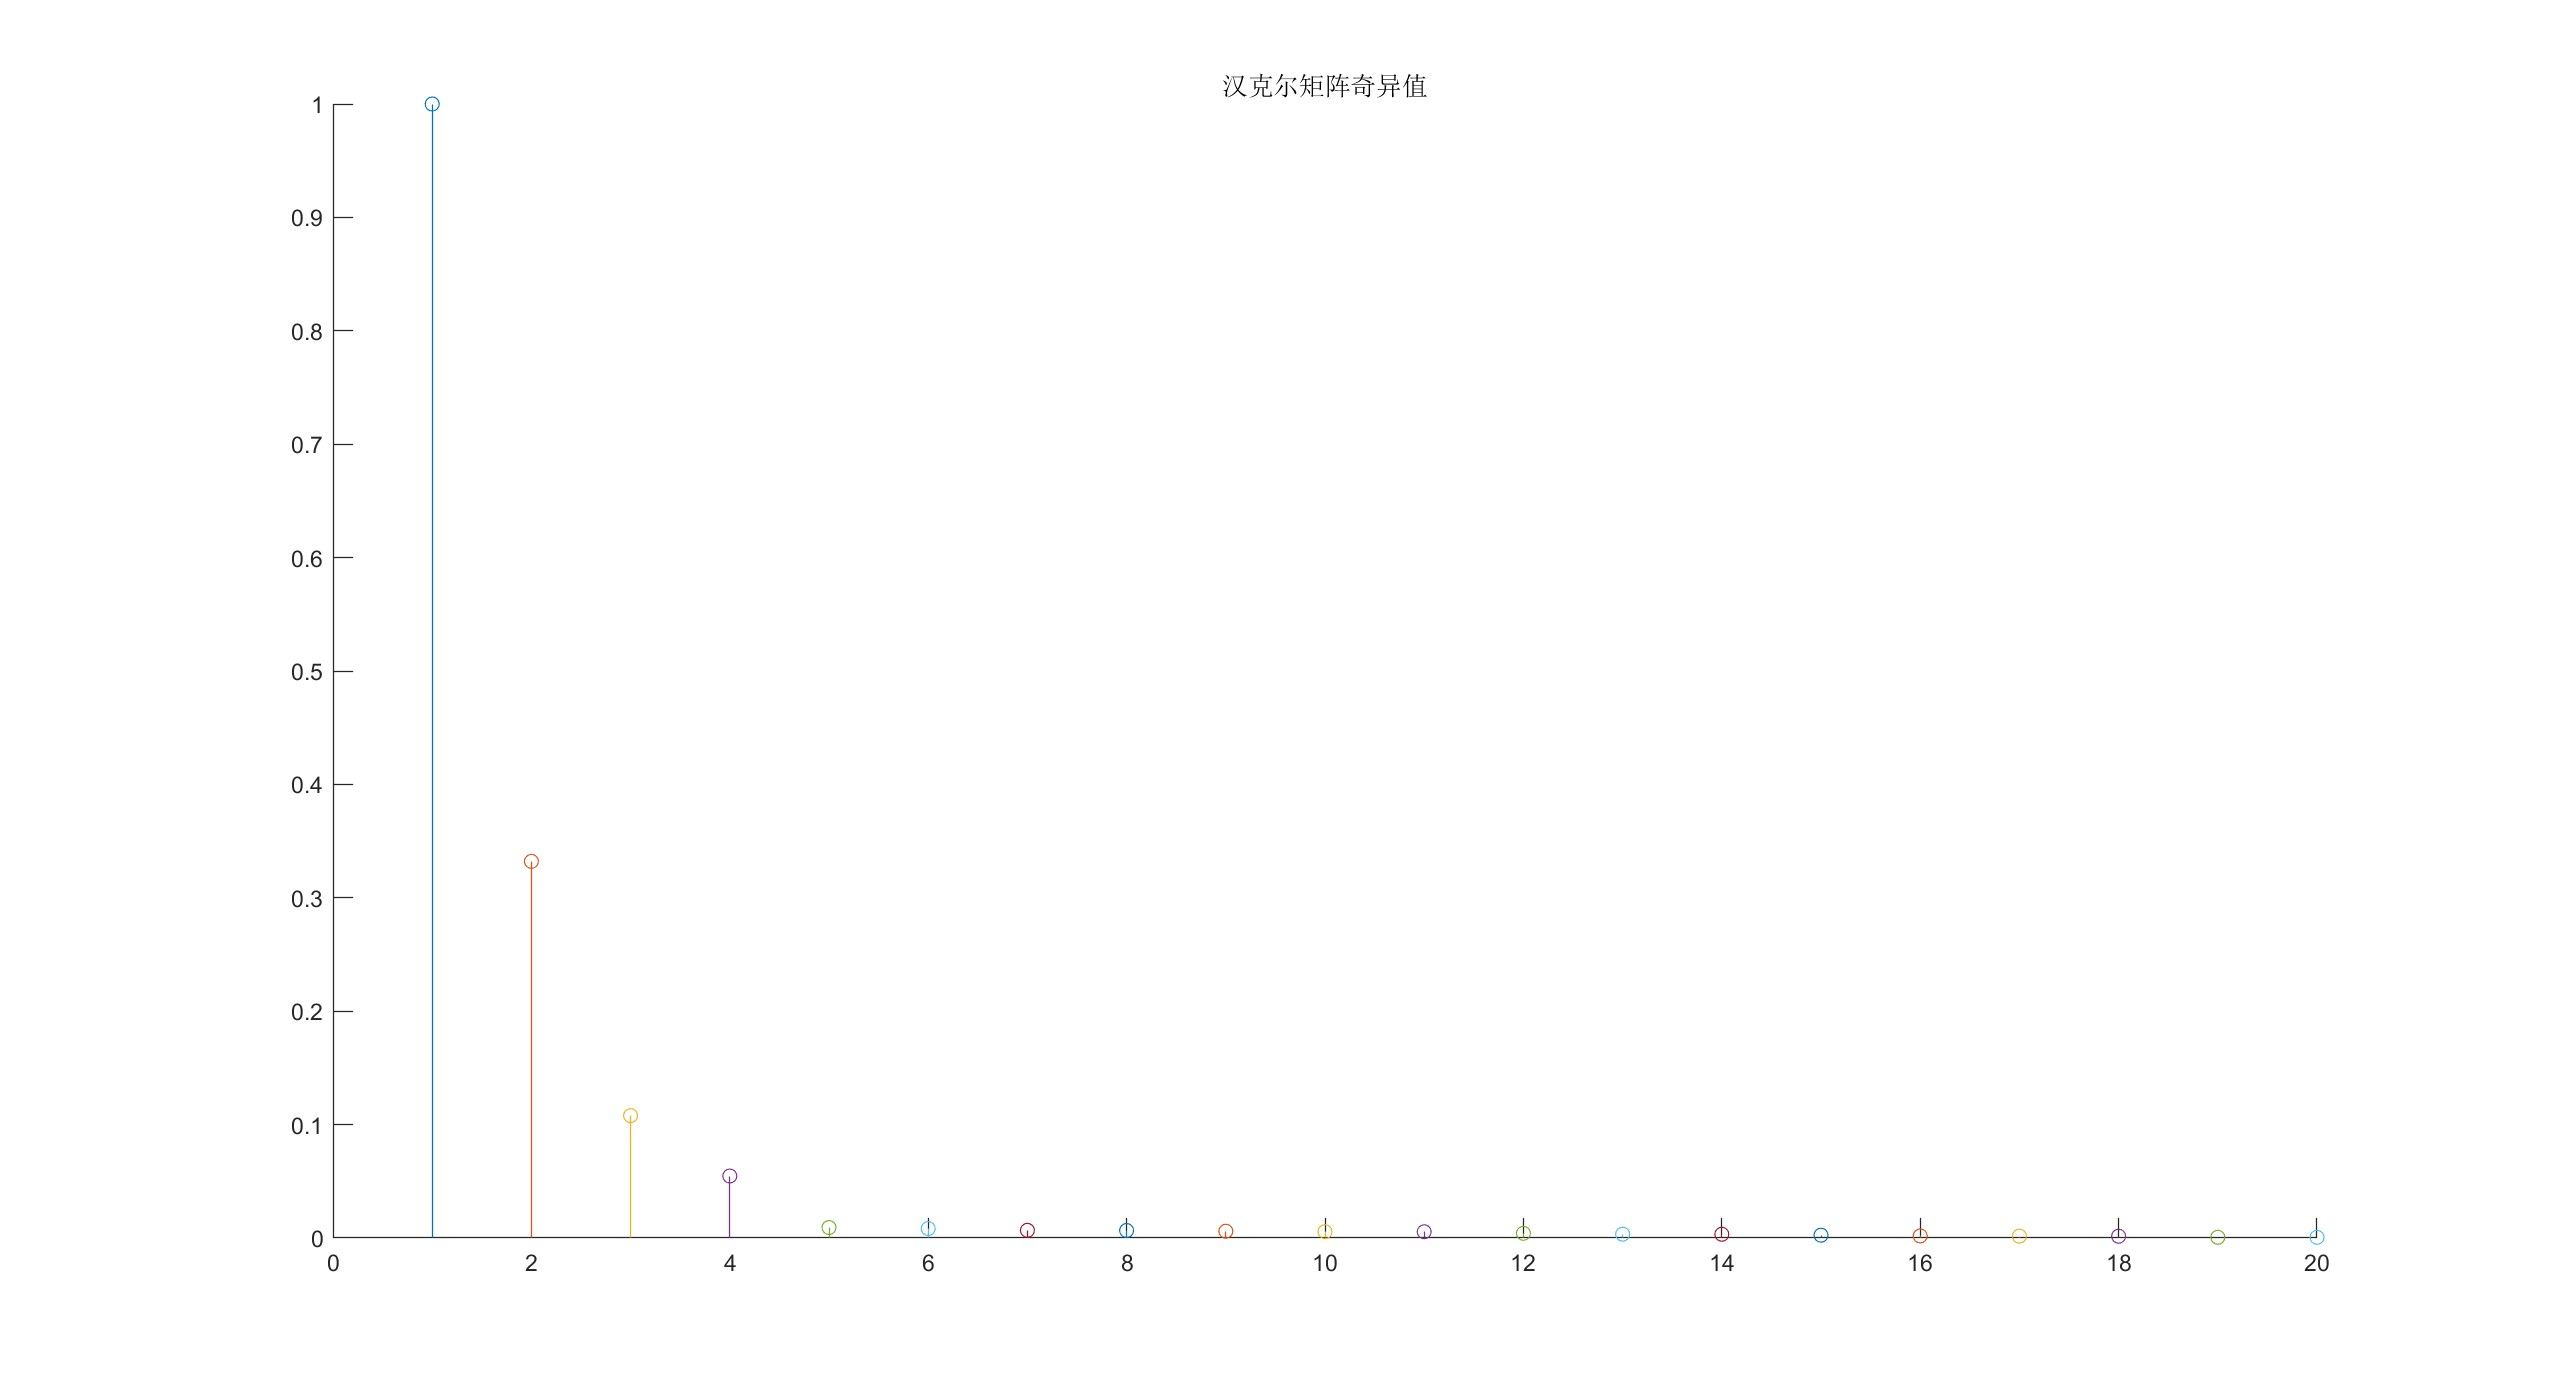
\includegraphics[width=\textwidth]
        {图片/机械堵转奇异值分解图.jpg}
        \caption{机械堵转奇异值分解图}
    \end{minipage}
    \begin{minipage}{0.5\textwidth}
        \centering
        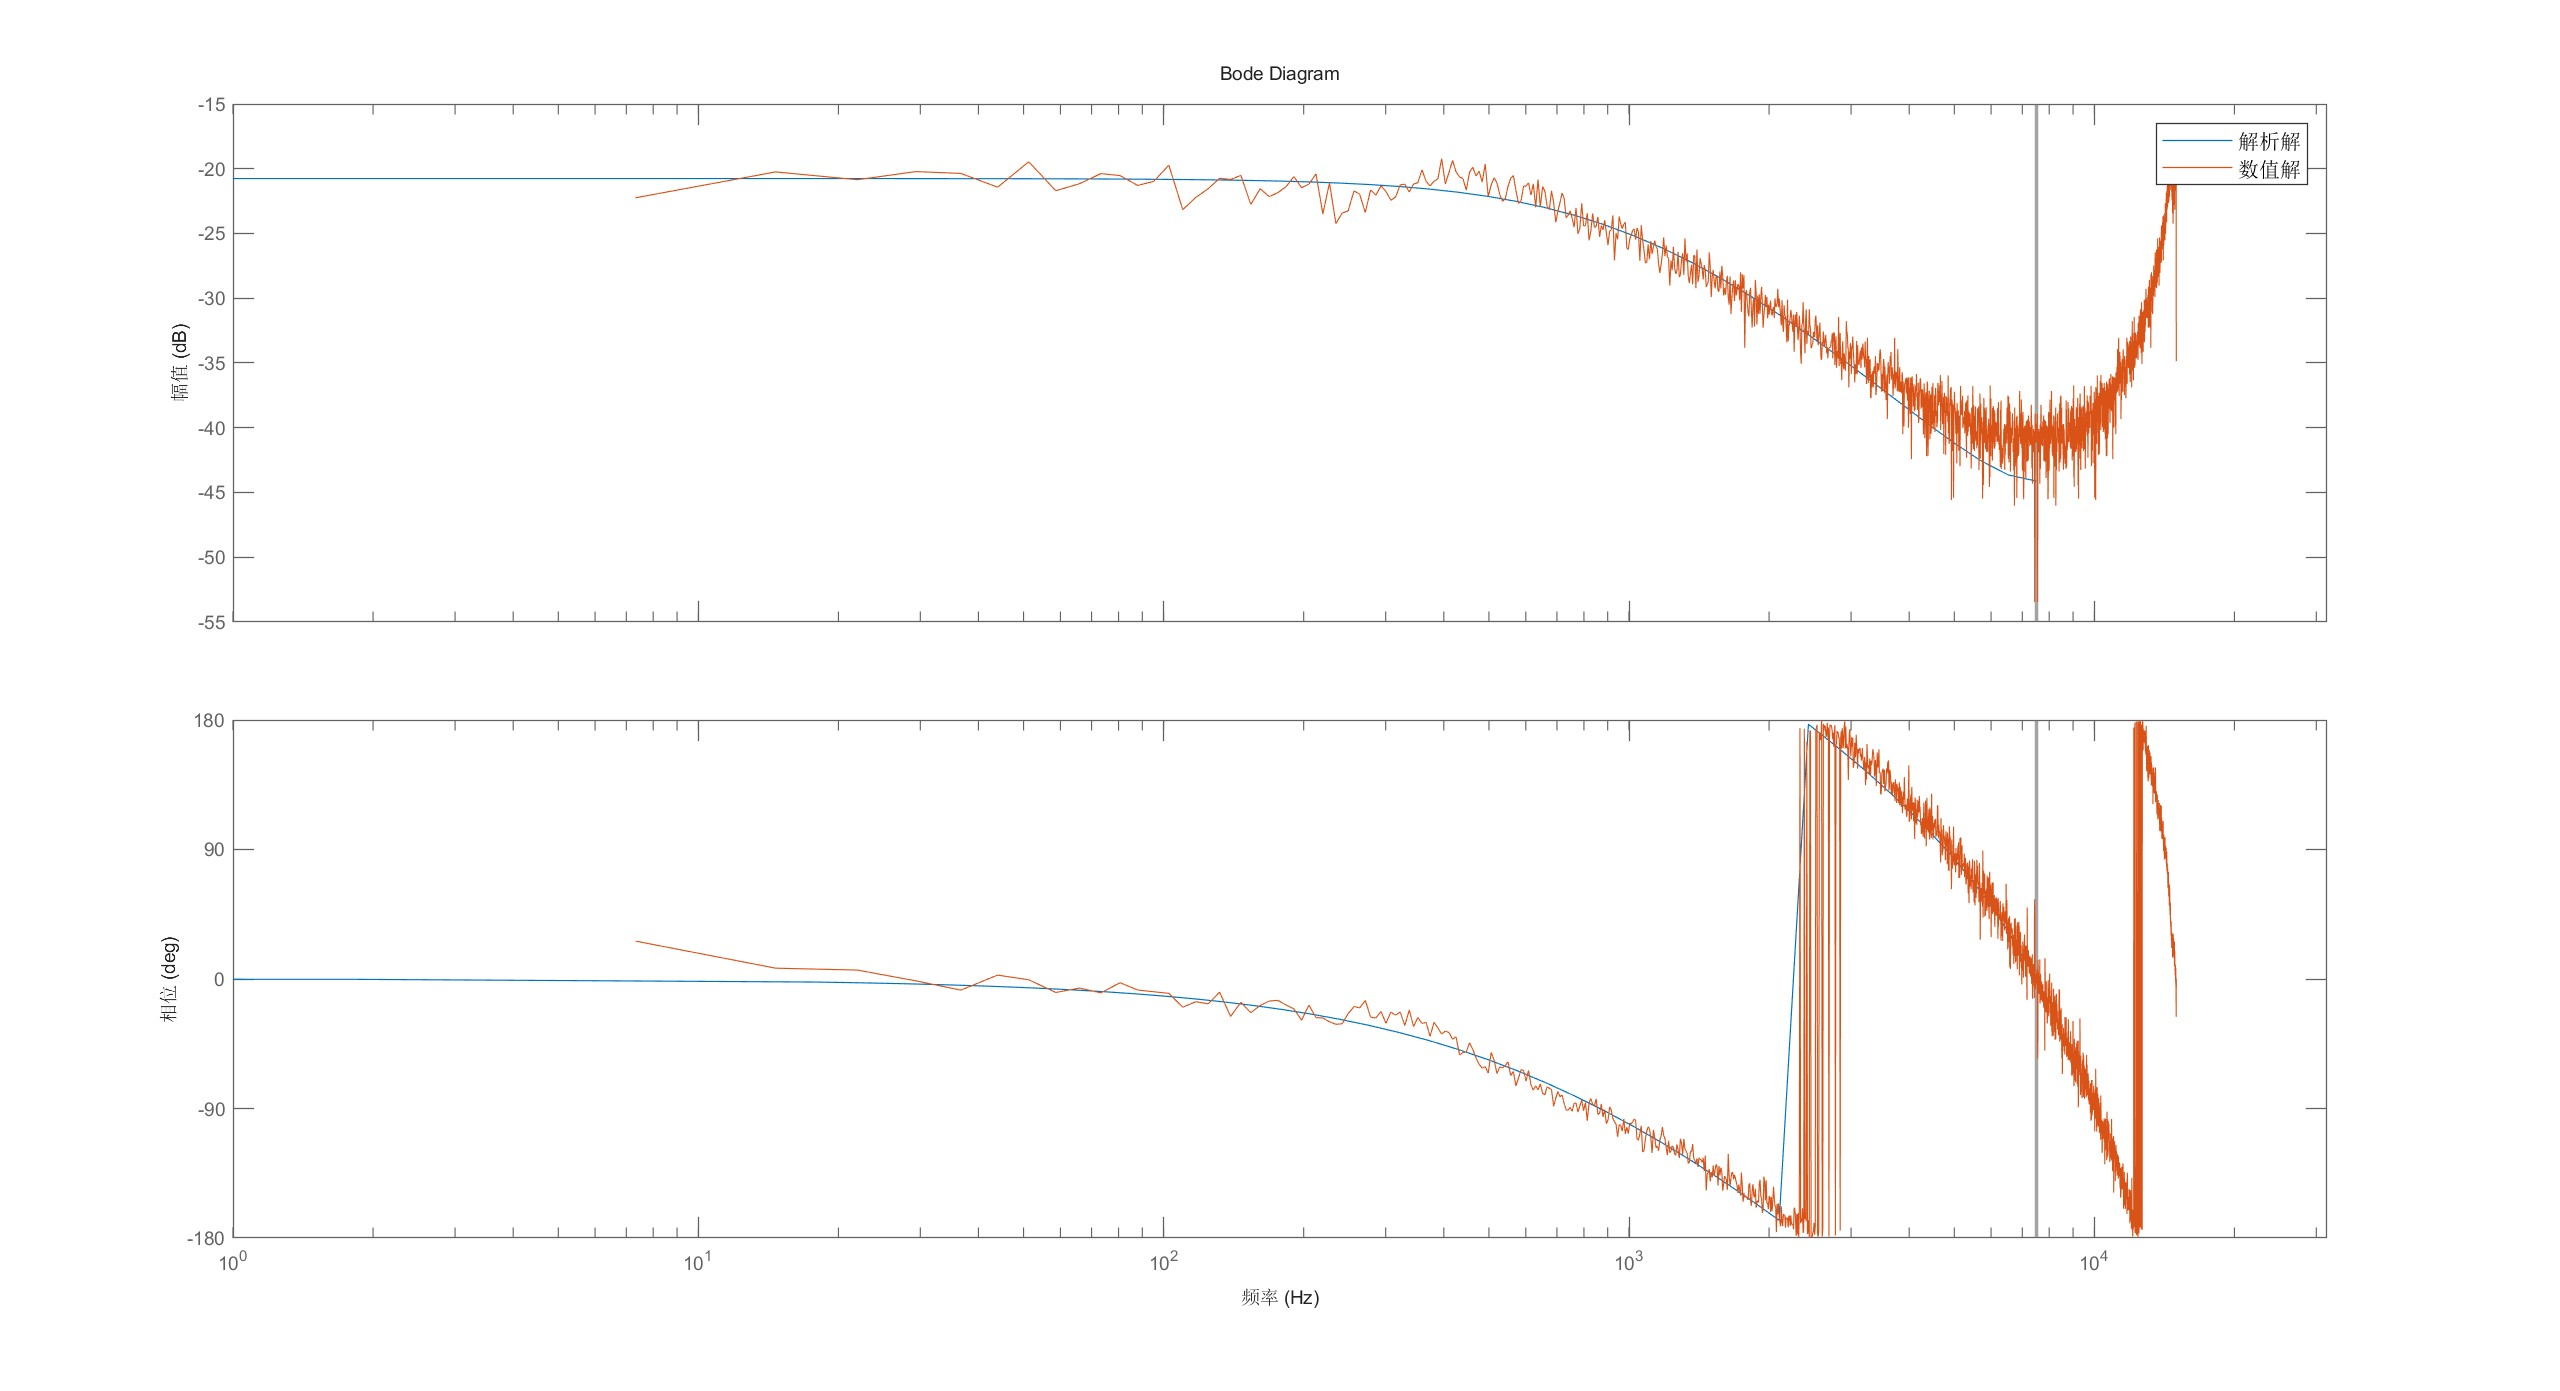
\includegraphics[width=\textwidth]
        {图片/机械堵转数值解与解析解对比.jpg}
        \caption{机械堵转数值解与解析解对比}
    \end{minipage}
\end{figure}

根据奇异值分解图，对比电气锁轴方式，可以发现系统阶次近似为二阶，转动耦合模态含量大大降低。传递函数辨识结果为
\(G(z)=\cfrac{-0.0000543  - 0.0002405 z^{-1} + 0.02709z^{-2}}{1 - 0.8149 z^{-1} + 0.0004799z^{-2}}\)，两个极点为
0.8143和0.0006。得到机械堵转下Q轴同步电感为\(L_q=1.85019\textrm{mH}\)。

上述结果看似合理，但是违背了电机的基本原理。根据D轴电感辨识结果\(L_{dO}=1.86152\textrm{mH}\)，结合相间电感估计Q轴同步电感范围
为\(L_q\in(2.13252,2.27211)\textrm{\textrm{mH}}\)，
Q轴电感需要满足\(L_q\ge 2.1\textrm{mH}\)，但是辨识结果为
\(L_{qO}\approx 1.86\textrm{mH}<2.1\textrm{mH}\)，认为是电机微动导致转动耦合模态没有完全消失，
而是和RL电路的模态融合成了一个极点，导致Q轴电感辨识不准确。

\subsubsection{数据后处理方法}
机械堵转和电气堵转都难以抵消运动模态带来的影响，最终选择后期数据处理。

通过后期补偿，在工作点0V附近进行HK辨识结果如下。可以发现，脉冲响应序列不再出现振荡。
\begin{figure}[H]
    \centering
    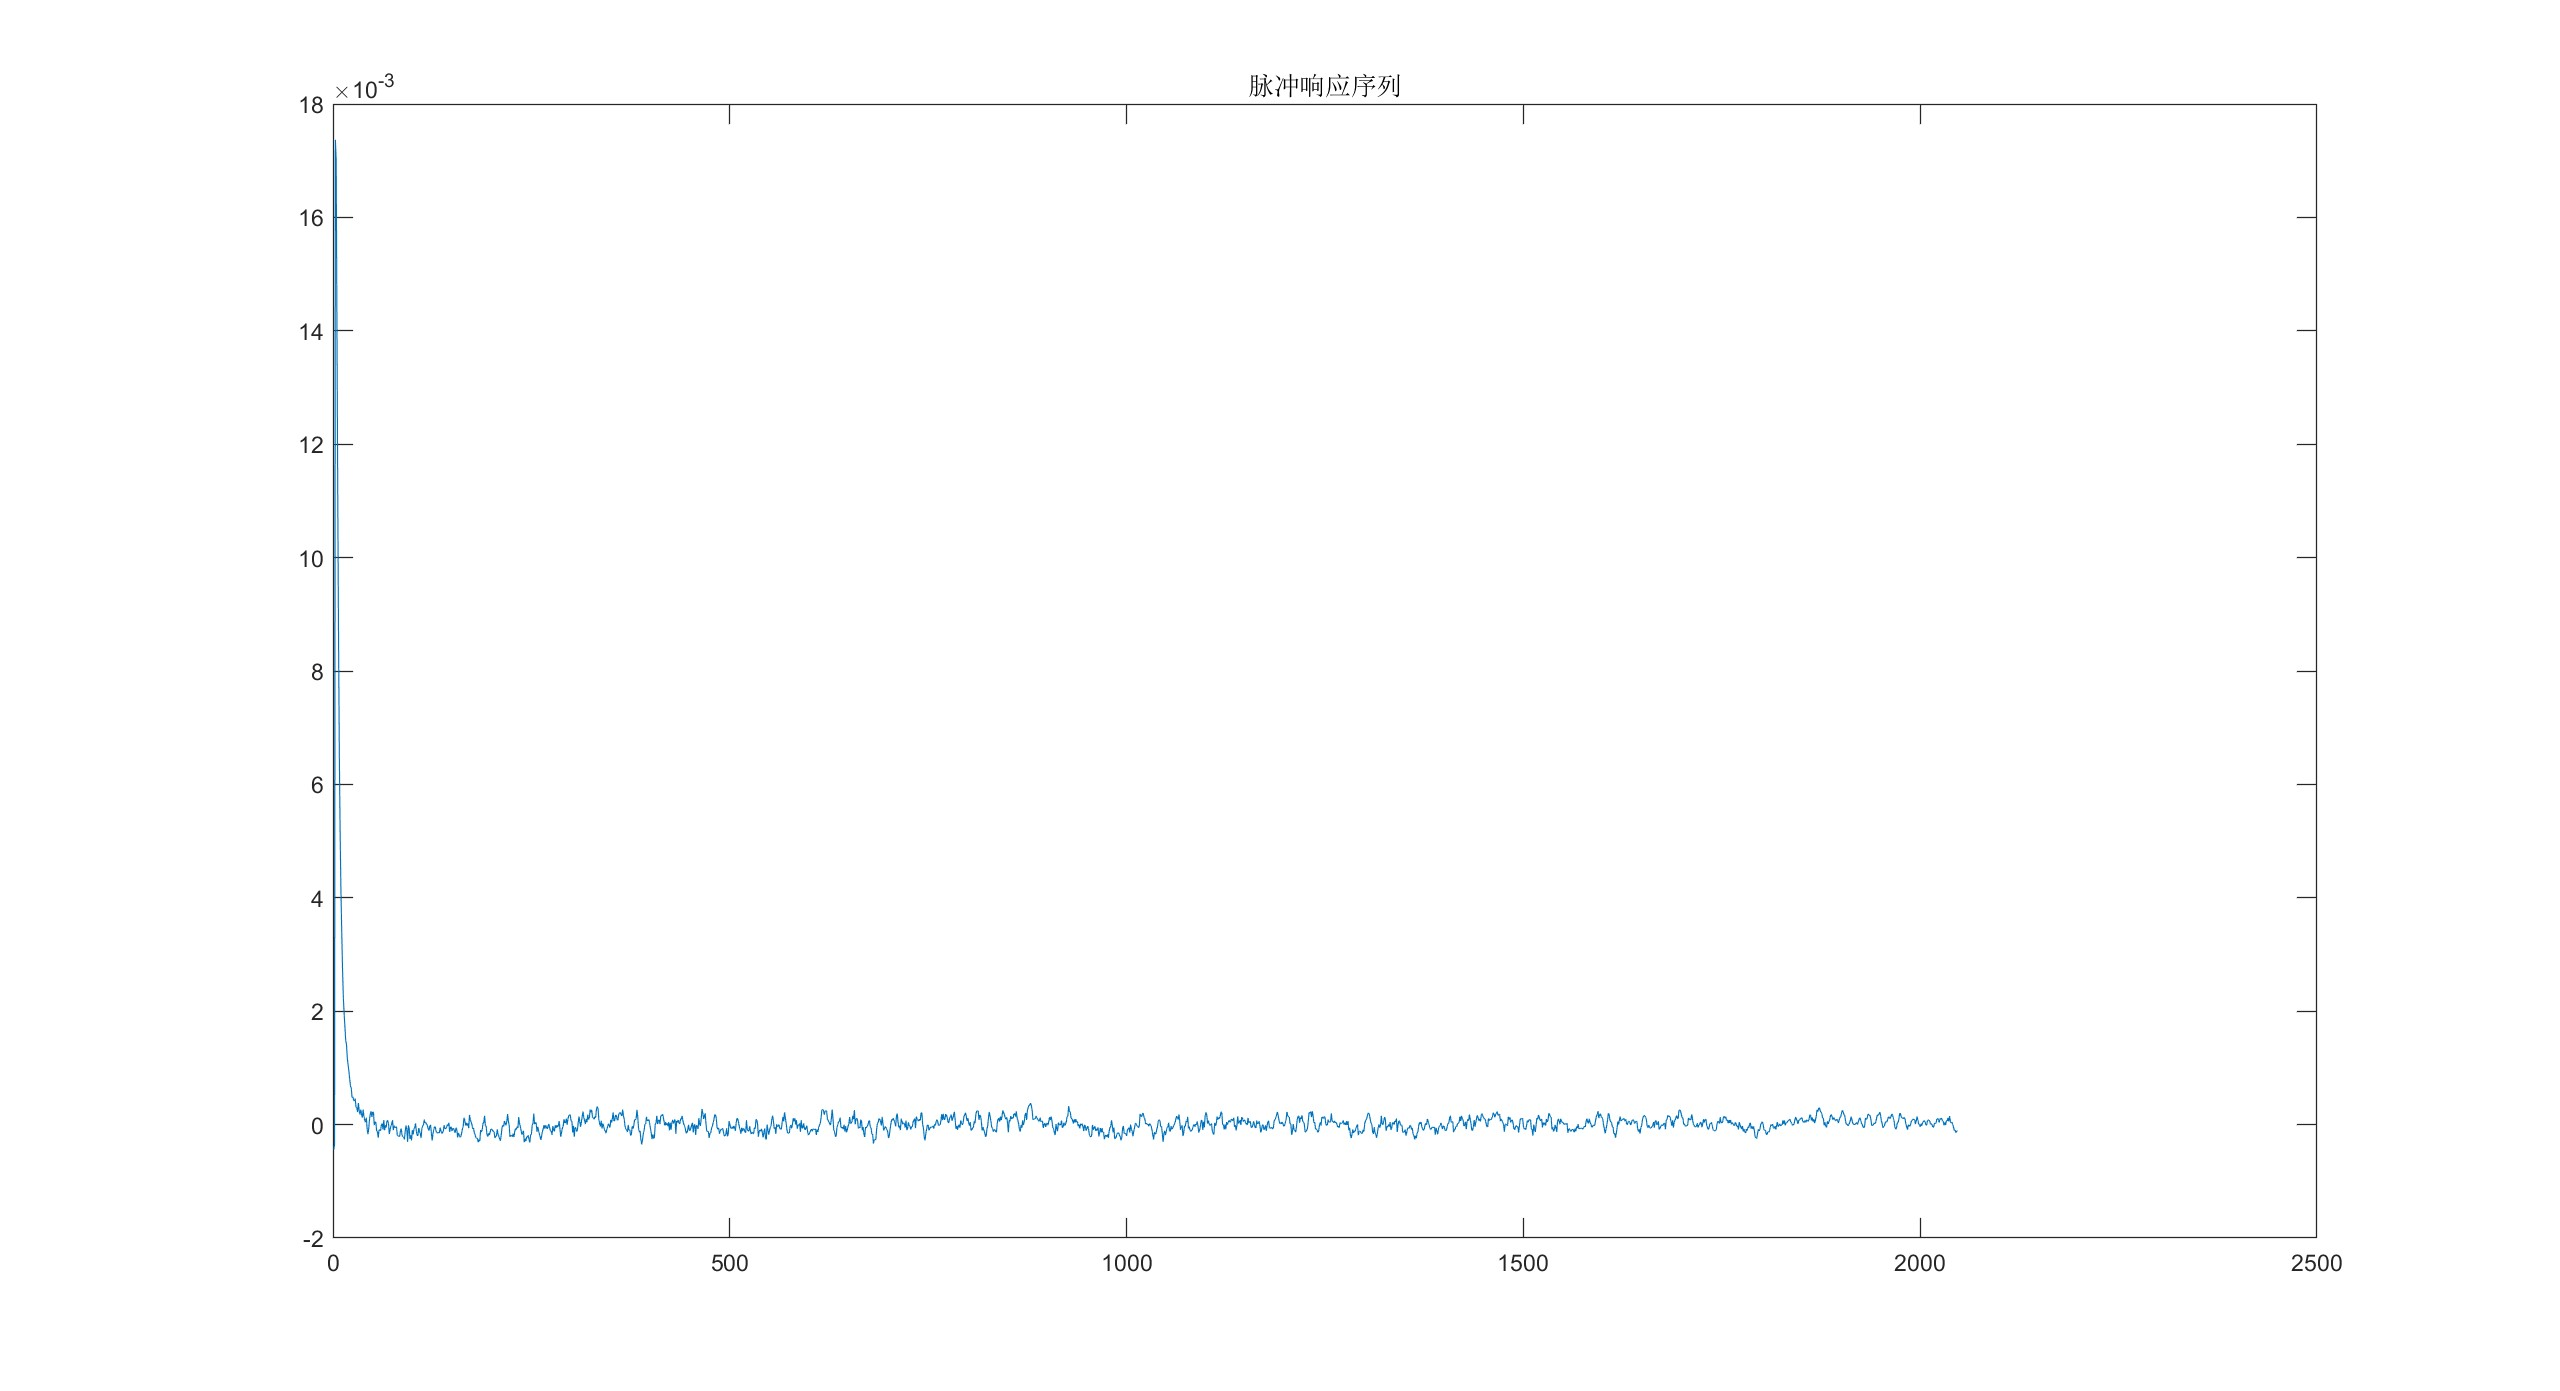
\includegraphics[width=0.5\textwidth]
    {图片/Q轴工作点0V脉冲响应序列.jpg}
    \caption{Q轴工作点0V脉冲响应序列}
\end{figure}

奇异值分解图和数值解解析解对比如下图所示。数值解与解析解的幅频相关系数为99.50080\(\%\)，
相频相关系数为99.97588\(\%\)，拟合优度90.81283\(\%\)。解析解传递函数为
\(G(z)=\cfrac{-0.000036  - 0.000101 z^{-1} + 0.0267z^{-2}}{1 - 0.8013 z^{-1} - 0.03188z^{-2}}\)，两个极点为
0.8393和-0.038。选取慢极点0.8393，根据\(L_q=-\cfrac{R_sT_s}{\ln(z_p)}\)计算Q轴电感为\(L_q=2.16828\textrm{mH}\)。
该辨识结果满足\(L_q\ge L_d\)，并且也满足相间电感估测结果\(L_q\in(2.13252,2.27211)\textrm{\textrm{mH}}\)。
\begin{figure}[H]
    \begin{minipage}{0.5\textwidth}
        \centering
        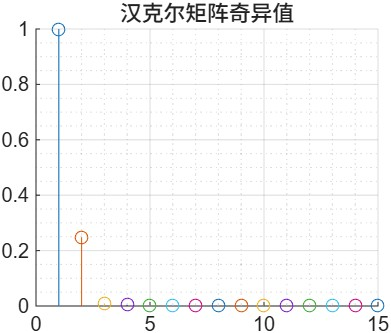
\includegraphics[width=\textwidth]
        {图片/Q轴工作点0V奇异值分解图.jpg}
        \caption{Q轴工作点0V奇异值分解图}
    \end{minipage}
    \begin{minipage}{0.5\textwidth}
        \centering
        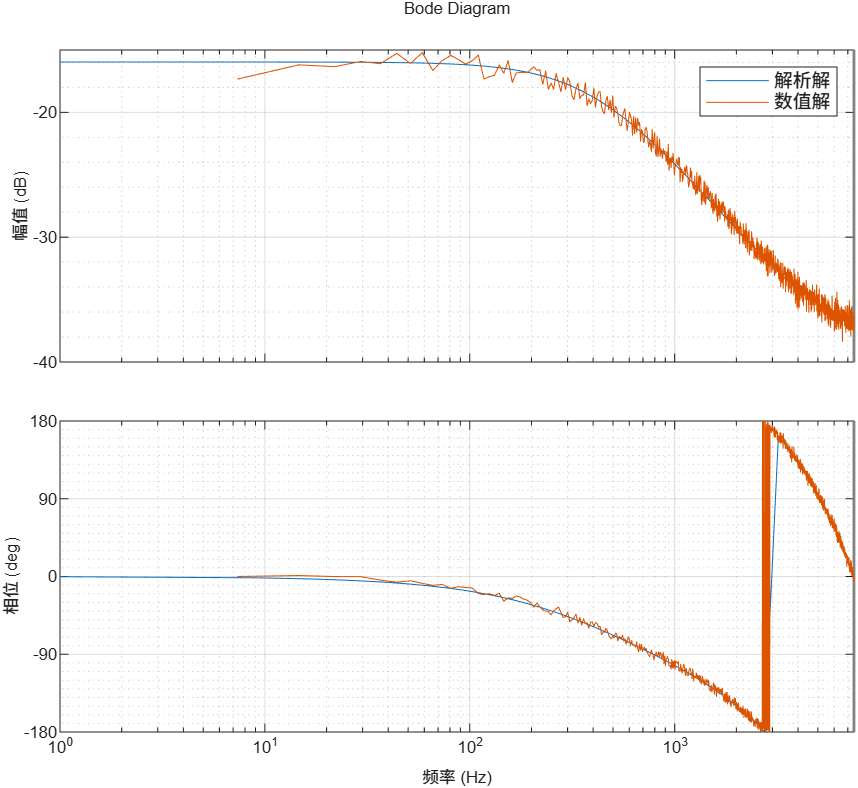
\includegraphics[width=\textwidth]
        {图片/Q轴工作点0V数值解和解析解对比.jpg}
        \caption{Q轴工作点0V数值解和解析解对比}
    \end{minipage}
\end{figure}

按照相同的方法，对工作点\(\pm2\)V、\(\pm4\)V进行辨识，结果如下。

工作点2V时，得到的Hankel矩阵奇异值分解和频域响应对比如下图所示。数值解与解析解的幅频相关系数为98.99637\(\%\)，
相频相关系数为99.95608\(\%\)，拟合优度84.70566\(\%\)。解析解传递函数为
\(G(z)=\cfrac{-0.0003126  - 0.0001889 z^{-1} + 0.02554z^{-2}}{1 - 0.8179 z^{-1} - 0.01559z^{-2}}\)，两个极点为
0.8365和-0.0186。得到2V工作点下Q轴同步电感为\(L_q=2.12868\textrm{mH}\)。
\begin{figure}[H]
    \begin{minipage}{0.5\textwidth}
        \centering
        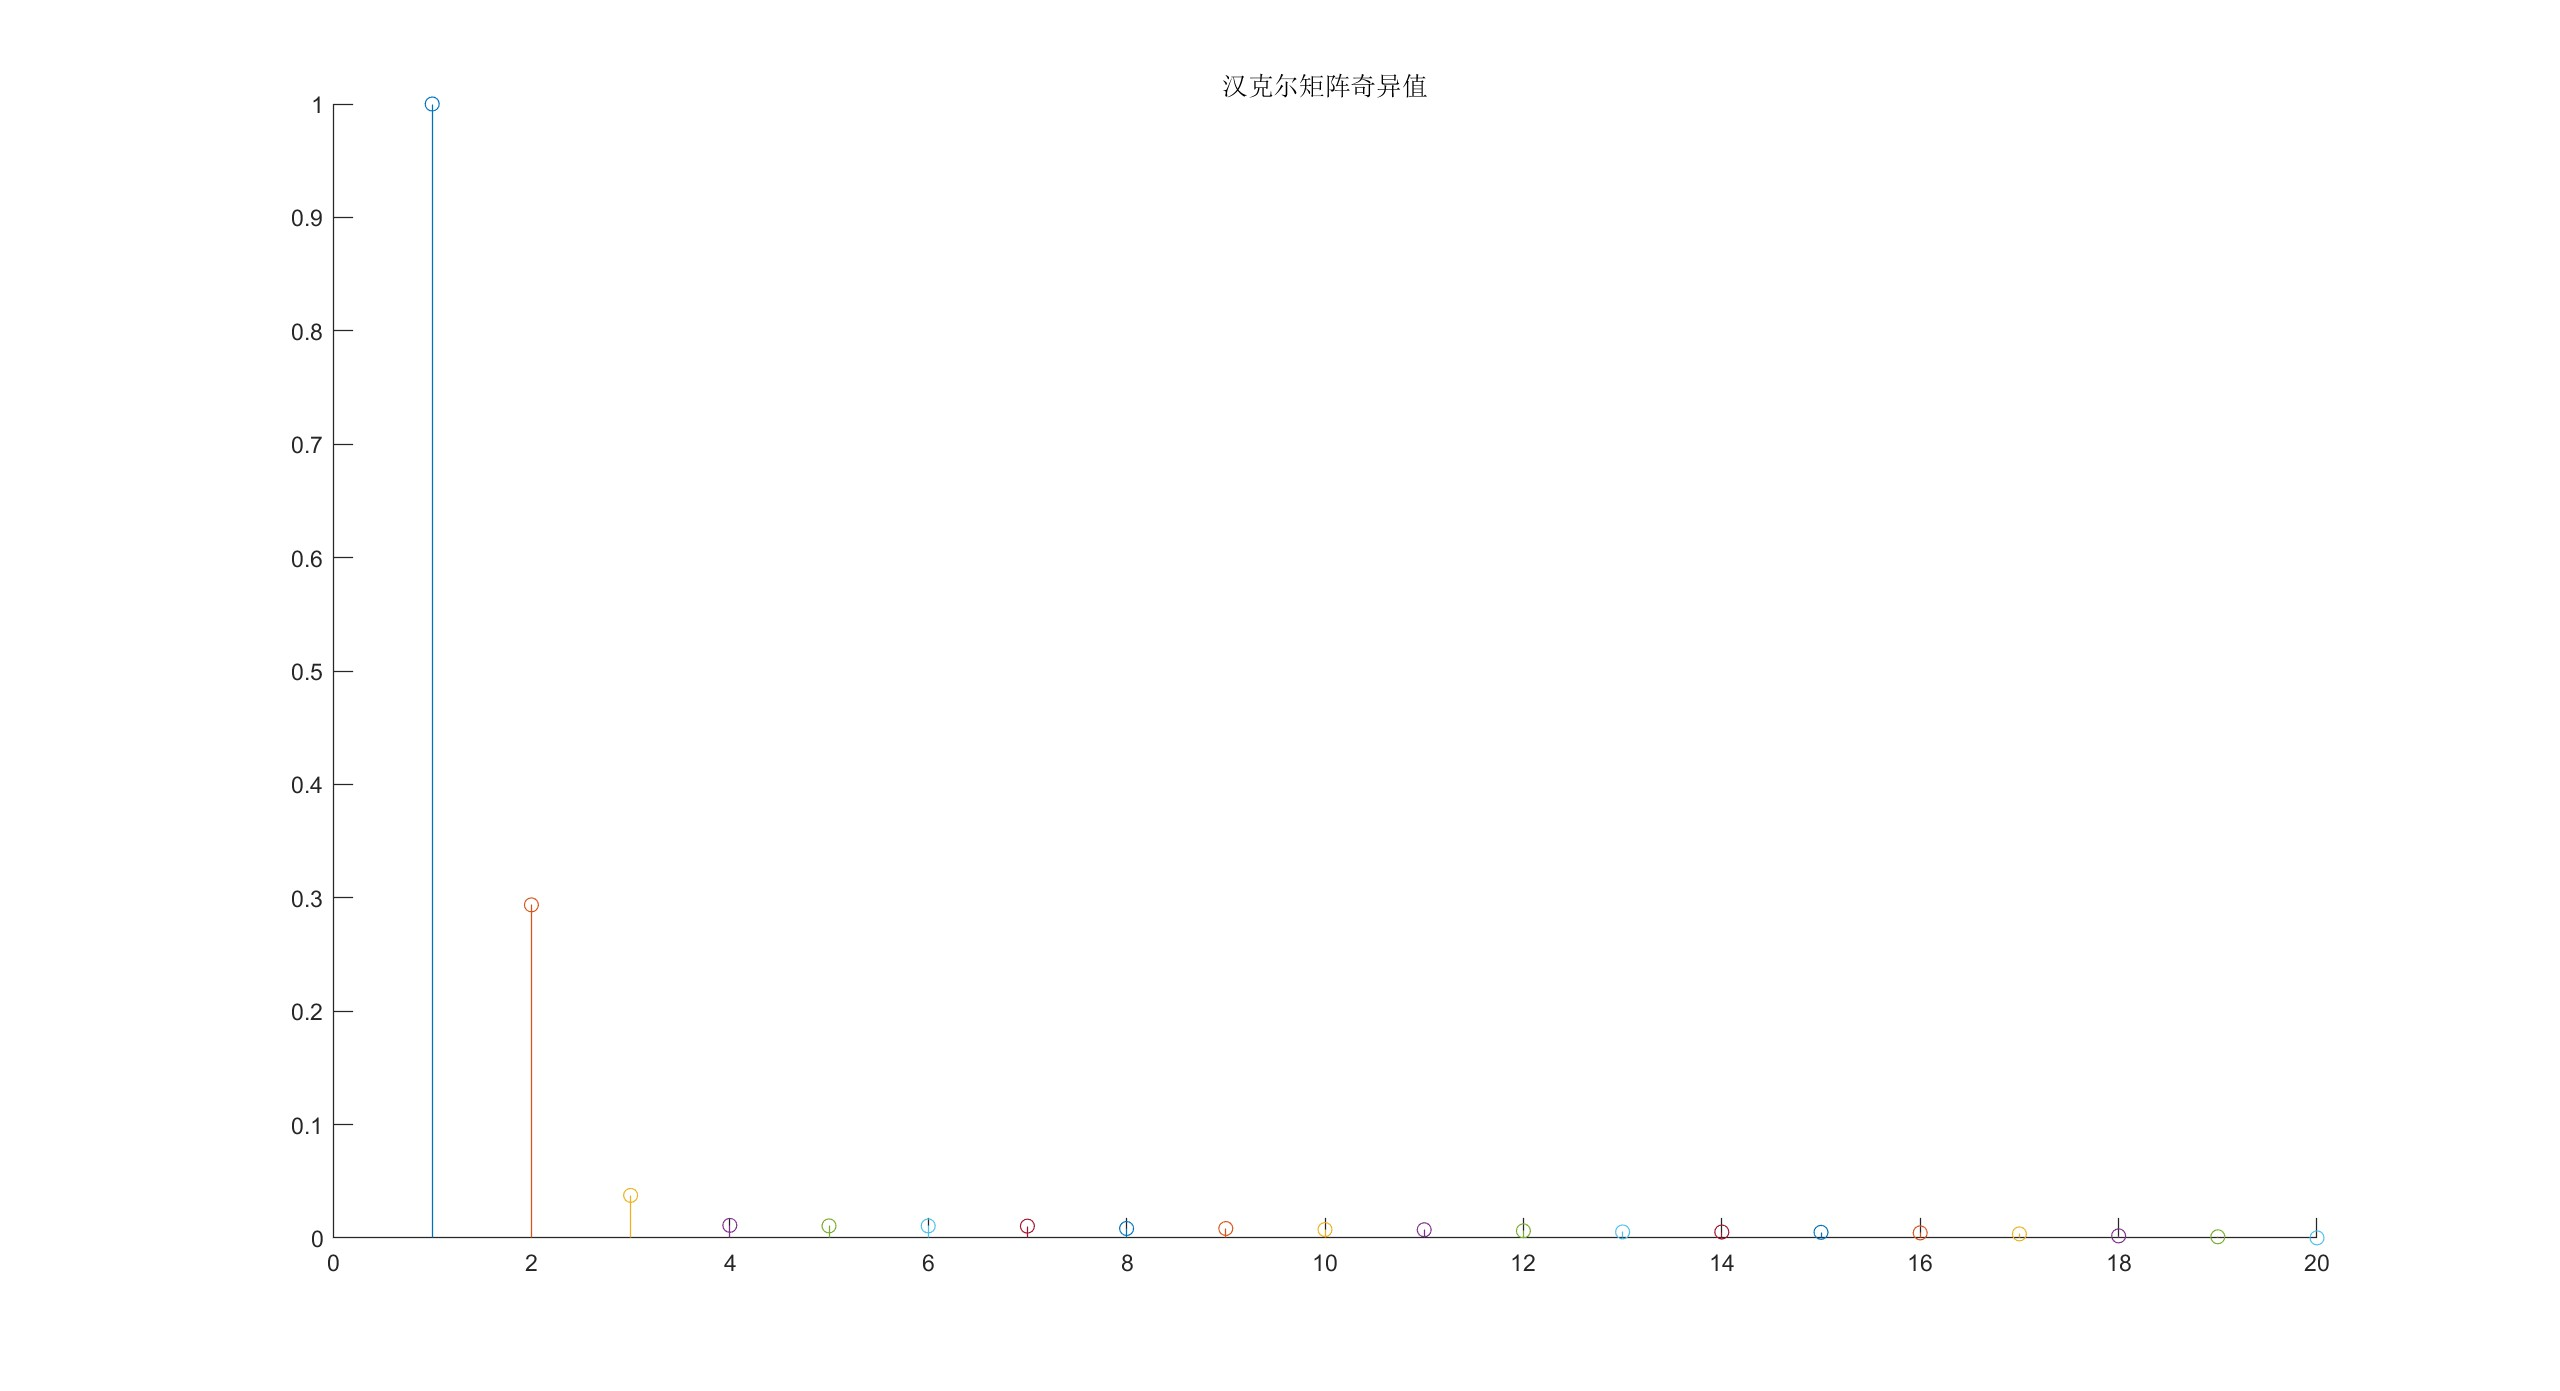
\includegraphics[width=\textwidth]
        {图片/Q轴工作点2V奇异值分解图.jpg}
        \caption{Q轴工作点2V奇异值分解图}
    \end{minipage}
    \begin{minipage}{0.5\textwidth}
        \centering
        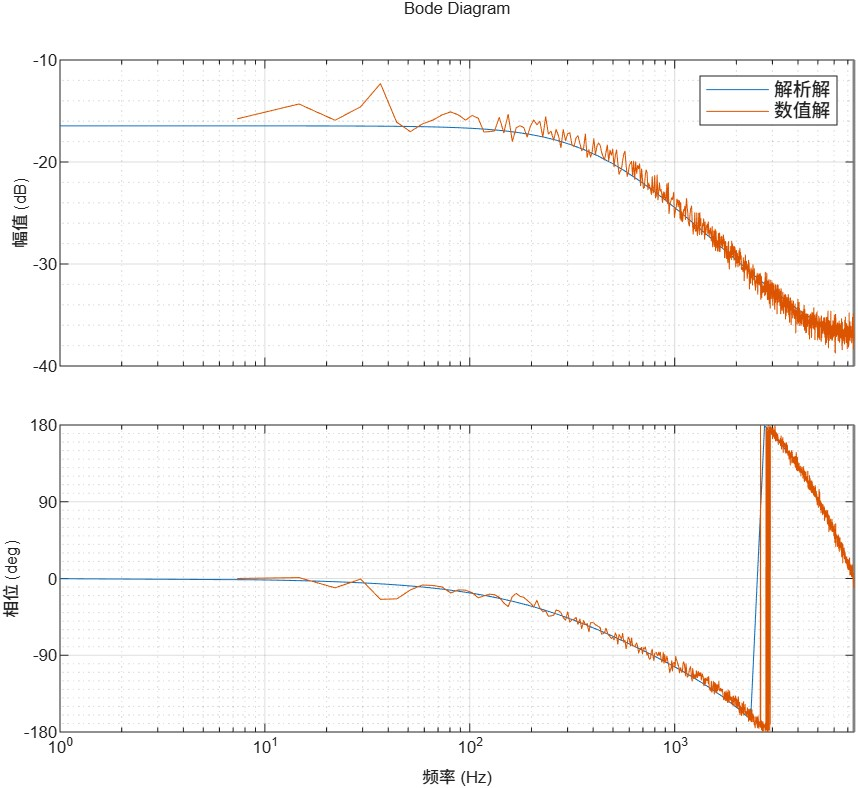
\includegraphics[width=\textwidth]
        {图片/Q轴工作点2V数值解和解析解对比.jpg}
        \caption{Q轴工作点2V数值解和解析解对比}
    \end{minipage}
\end{figure}

工作点4V时，得到的Hankel矩阵奇异值分解和频域响应对比如下图所示。数值解与解析解的幅频相关系数为98.65486\(\%\)，
相频相关系数为99.94388\(\%\)，拟合优度82.84616\(\%\)。解析解传递函数为
\(G(z)=\cfrac{-0.0003139  + 0.0001031 z^{-1} + 0.02462z^{-2}}{1 - 0.837 z^{-1} - 0.004508z^{-2}}\)，两个极点为
0.8424和-0.0054。得到4V工作点下Q轴同步电感为\(L_q=2.21481\textrm{mH}\)。
\begin{figure}[H]
    \begin{minipage}{0.5\textwidth}
        \centering
        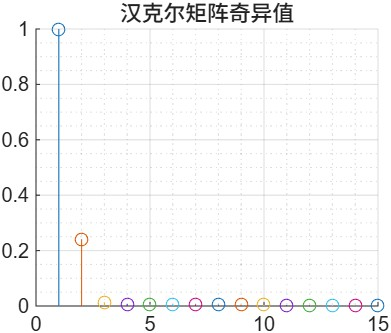
\includegraphics[width=\textwidth]
        {图片/Q轴工作点4V奇异值分解图.jpg}
        \caption{Q轴工作点4V奇异值分解图}
    \end{minipage}
    \begin{minipage}{0.5\textwidth}
        \centering
        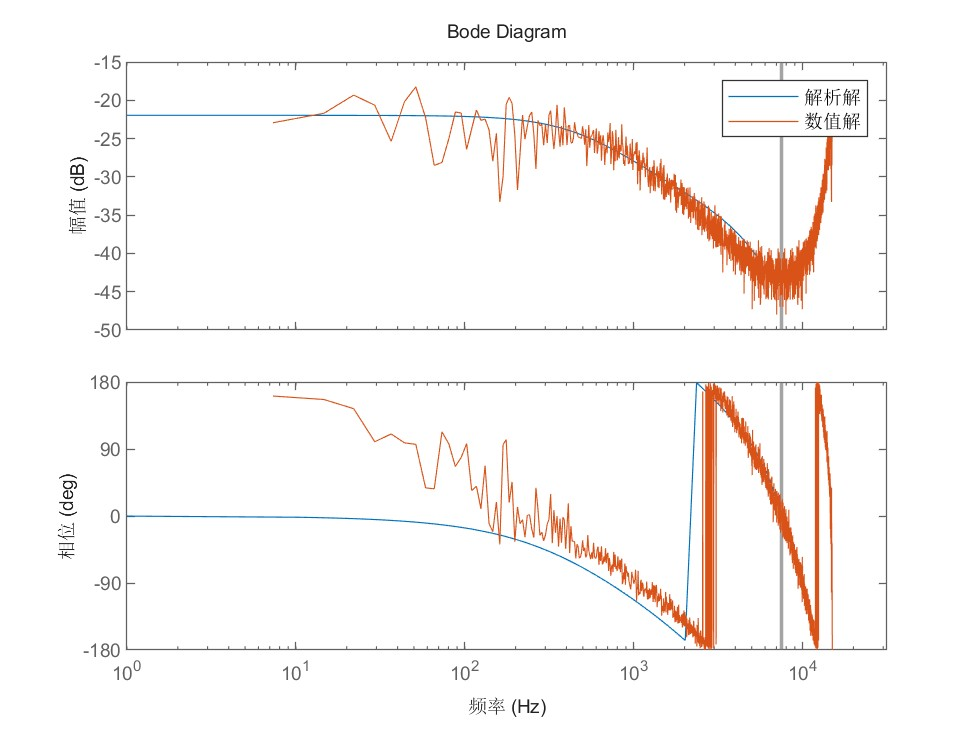
\includegraphics[width=\textwidth]
        {图片/Q轴工作点4V数值解和解析解对比.jpg}
        \caption{Q轴工作点4V数值解和解析解对比}
    \end{minipage}
\end{figure}

工作点-2V时，得到的Hankel矩阵奇异值分解和频域响应对比如下图所示。数值解与解析解的幅频相关系数为99.00722\(\%\)，
相频相关系数为99.97406\(\%\)，拟合优度86.66177\(\%\)。解析解传递函数为
\(G(z)=\cfrac{-0.00007114  + 0.00005972 z^{-1} + 0.02562z^{-2}}{1 - 0.8119 z^{-1} - 0.0271z^{-2}}\)，两个极点为
0.8440和-0.0321。得到-2V工作点下Q轴同步电感为\(L_q=2.24055\textrm{mH}\)。
\begin{figure}[H]
    \begin{minipage}{0.5\textwidth}
        \centering
        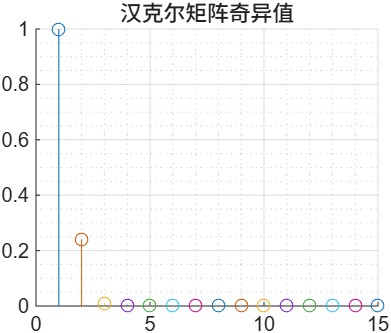
\includegraphics[width=\textwidth]
        {图片/Q轴工作点-2V奇异值分解图.jpg}
        \caption{Q轴工作点-2V奇异值分解图}
    \end{minipage}
    \begin{minipage}{0.5\textwidth}
        \centering
        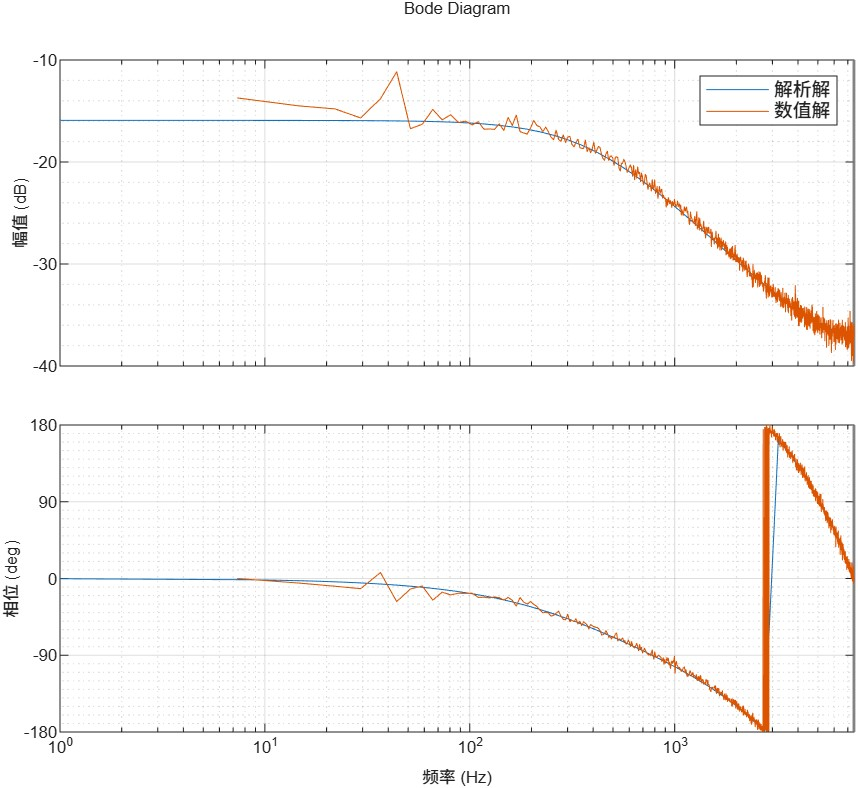
\includegraphics[width=\textwidth]
        {图片/Q轴工作点-2V数值解和解析解对比.jpg}
        \caption{Q轴工作点-2V数值解和解析解对比}
    \end{minipage}
\end{figure}

工作点-4V时，得到的Hankel矩阵奇异值分解和频域响应对比如下图所示。数值解与解析解的幅频相关系数为99.24784\(\%\)，
相频相关系数为99.96070\(\%\)，拟合优度86.58094\(\%\)。解析解传递函数为
\(G(z)=\cfrac{-0.00003683 - 0.0002048 z^{-1} + 0.02451z^{-2}}{1 - 0.8267 z^{-1} - 0.01035z^{-2}}\)，两个极点为
0.8309和-0.0123。得到-4V工作点下Q轴同步电感为\(L_q=2.16473\textrm{mH}\)。
\begin{figure}[H]
    \begin{minipage}{0.5\textwidth}
        \centering
        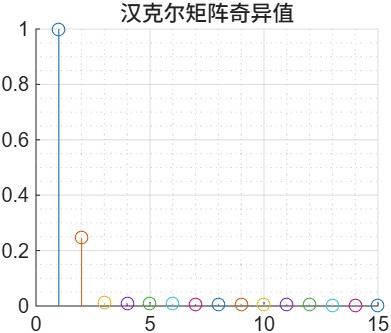
\includegraphics[width=\textwidth]
        {图片/Q轴工作点-4V奇异值分解图.jpg}
        \caption{Q轴工作点-4V奇异值分解图}
    \end{minipage}
    \begin{minipage}{0.5\textwidth}
        \centering
        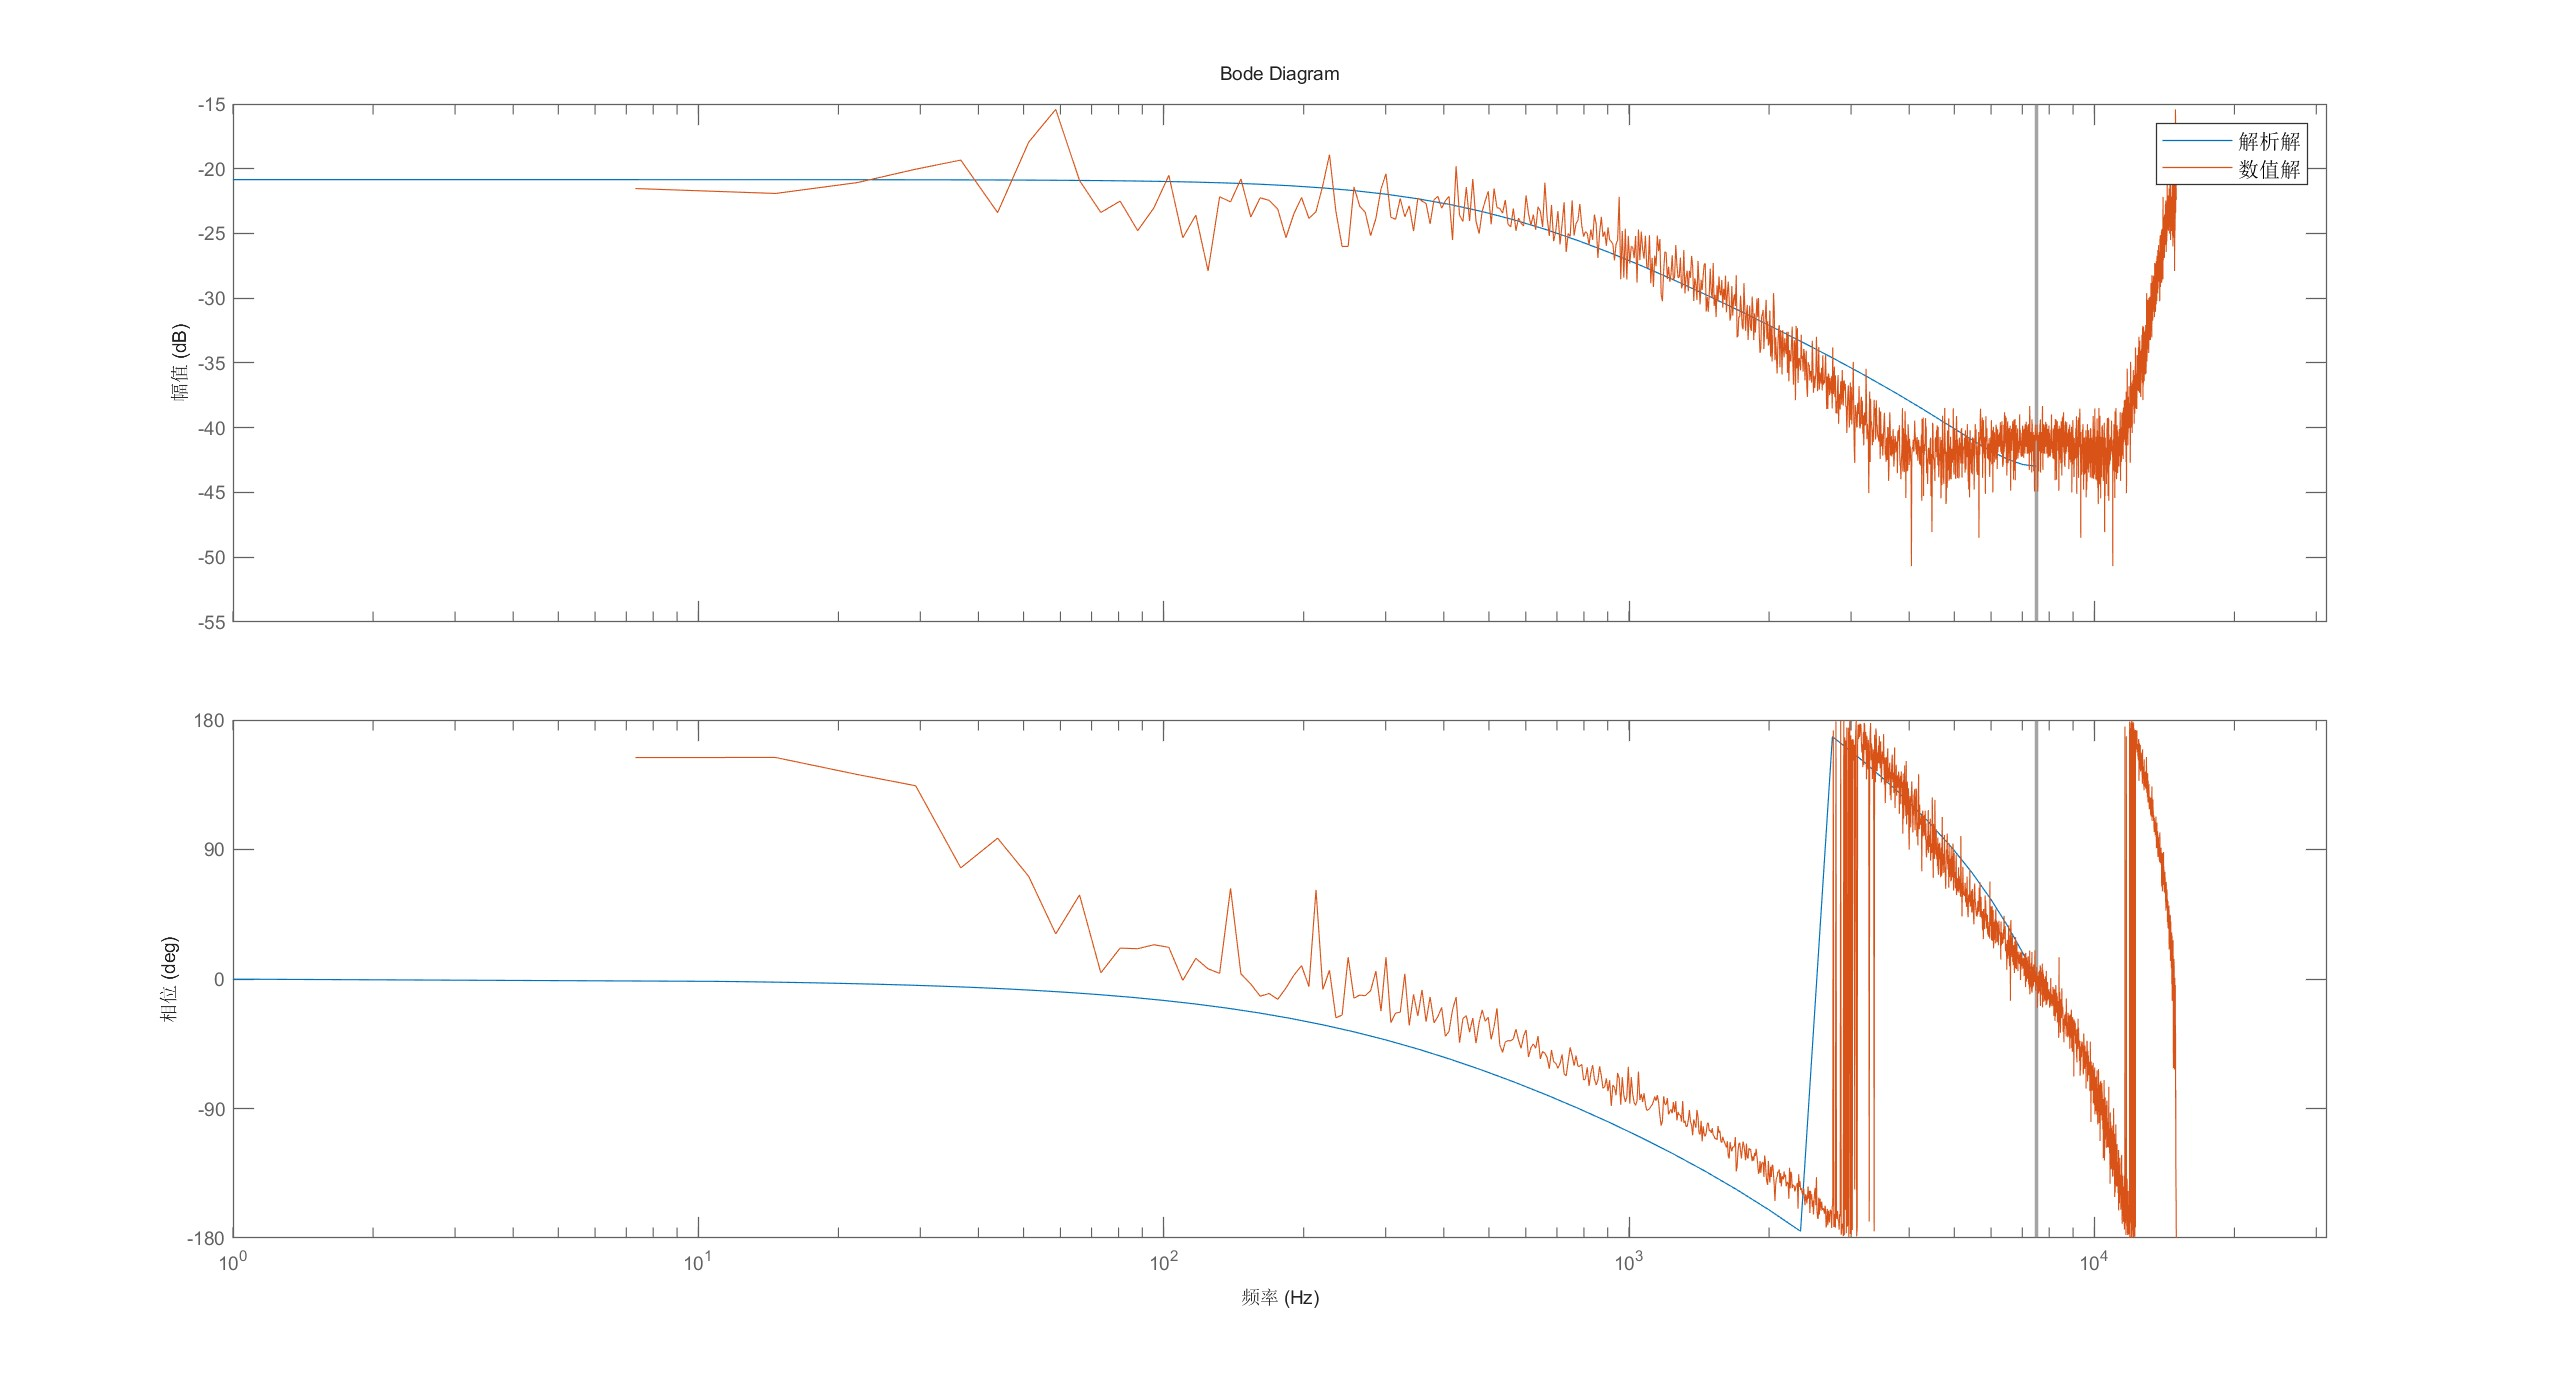
\includegraphics[width=\textwidth]
        {图片/Q轴工作点-4V数值解和解析解对比.jpg}
        \caption{Q轴工作点-4V数值解和解析解对比}
    \end{minipage}
\end{figure}

将上述五个工作点的Q轴辨识结果汇总如下表所示。
\begin{table}[H]
    \centering
    \begin{tabular}{|c|c|c|c|c|}
        \hline
        工作点 & 幅频相关系数 & 相频相关系数 & 拟合优度 & \(L_q\)辨识值（mH）\\
        \hline
        \(U_q=-4\text{V}\)  & 99.24784\% & 99.96070\% & 86.58094\% & 2.16473\\
        \hline
        \(U_q=-2\text{V}\)  & 99.00722\% & 99.97406\% & 86.66177\% & 2.24055\\
        \hline
        \(U_q=0\text{V}\)   & 99.50080\% & 99.97588\% & 90.81283\% & 2.16828\\
        \hline
        \(U_q=2\text{V}\)   & 98.99637\% & 99.95608\% & 84.70566\% & 2.12868\\
        \hline
        \(U_q=4\text{V}\)   & 98.65486\% & 99.94388\% & 82.84616\% & 2.21481\\
        \hline
    \end{tabular}
    \caption{Q轴各工作点HK辨识结果汇总}
    \label{tab:Q轴各工作点辨识结果汇总}
\end{table}

可以发现，随着工作点绝对值升高，数值解与解析解的相关系数快速降低。
推测是因为随着工作点绝对值升高，转速也随之升高，齿槽力、摩擦力等非线性因素
影响升高到不可忽略的地步，他们干扰了对Q轴同步电感的辨识。因此选择在工作点0V时的辨识结果作为最终结果：
\begin{equation*}
    L_{qO}=2.16828\textrm{mH}
\end{equation*}

\subsection{辨识模型验证}
根据相电阻和同步电感的辨识结果，结合PWM延迟和逆变器惯性，使用零阶保持器ZOH可以构建DQ轴传递函数：
\begin{equation*}
    \begin{cases}
        G_D(z)=(1-z^{-1})\mathcal{Z}[\cfrac{e^{-66.93\times10^{-6}s}}
        {s(5.70125+1.86152\times 10^{-3}s)(120\times 10^{-9}s+1)}]\\
        G_Q(z)=(1-z^{-1})\mathcal{Z}[\cfrac{e^{-66.93\times10^{-6}s}}
        {s(5.70125+2.16828\times 10^{-3}s)(120\times 10^{-9}s+1)}]
    \end{cases}
\end{equation*}

选用幅值为±5V的方波信号作为激励信号，分别输入到\(U_d\)和\(U_q\)，在电机空载的情况下记录D轴和Q轴的实际响应
并用上述传递函数计算仿真响应。其中由于Q轴在空载时存在电磁转矩，电机会转动产生反电动势，因此同样使用
数据处理方法计算等效输入到Q轴RL电路的电压\(U_q'=U_q-\omega_e(L_di_d+\psi_m)\)。

首先对D轴进行测试，结果如下。
\begin{figure}[H]
    \centering
    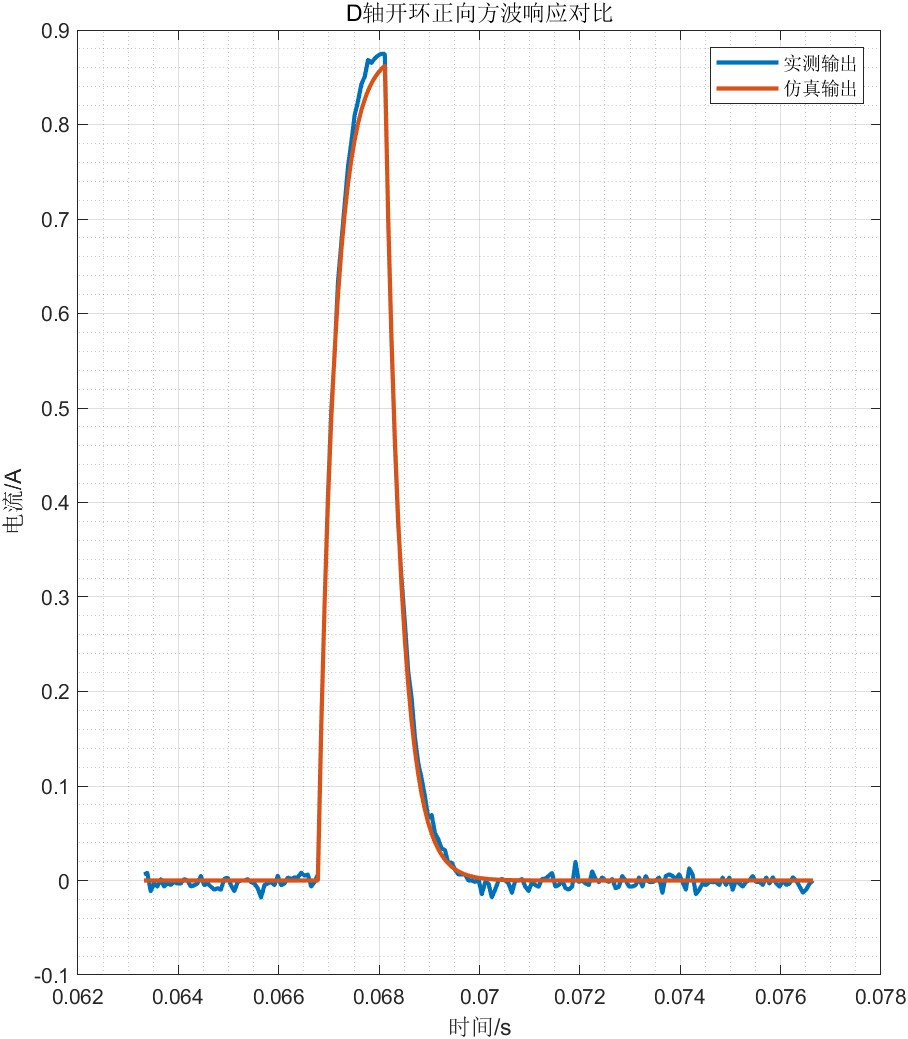
\includegraphics[width=\textwidth]
    {图片/D轴模型验证（正向）.jpg}
    \caption{D轴正向方波模型验证}
\end{figure}
\begin{figure}[H]
    \centering
    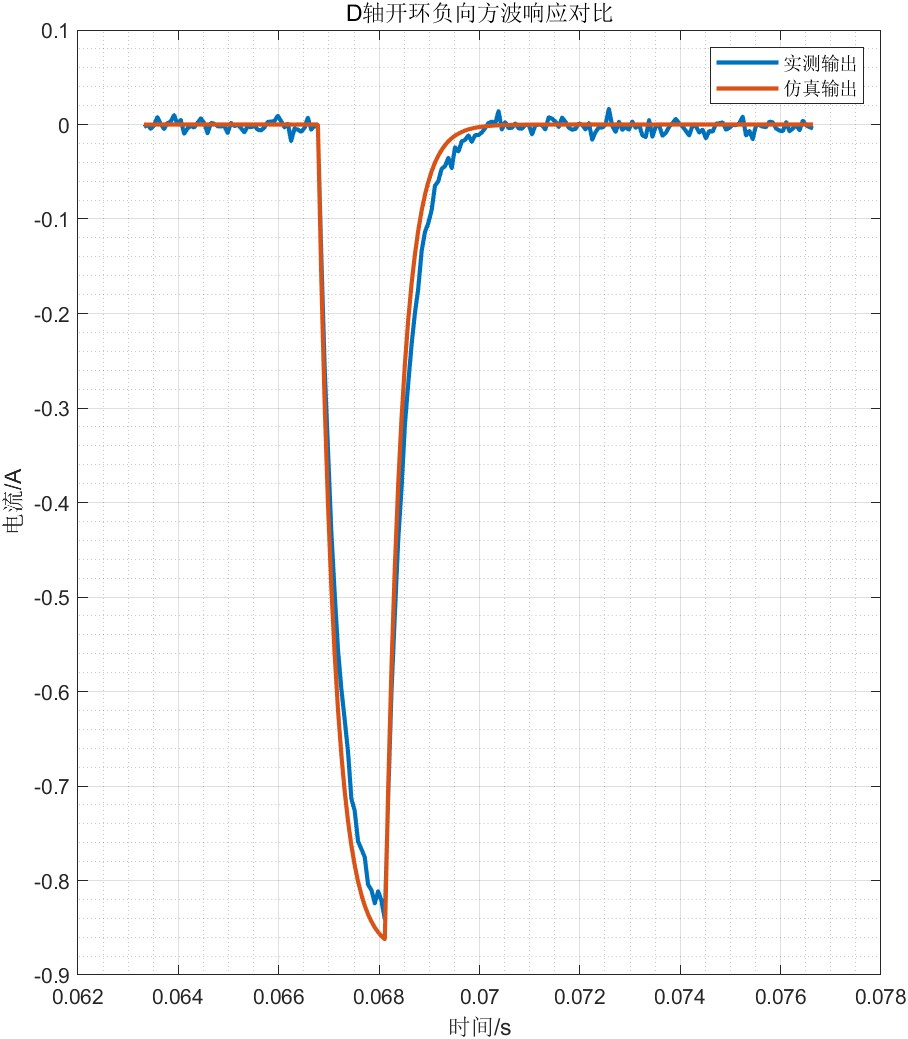
\includegraphics[width=\textwidth]
    {图片/D轴模型验证（负向）.jpg}
    \caption{D轴负向方波模型验证}
\end{figure}

根据响应曲线可以发现，D轴实测曲线和仿真曲线之间存在直流偏置（加性误差）。
尽管在程序初始化时于空载条件下测量了ADC偏置并加以扣除，但负载运行时电阻
因过电流温升导致的阻值漂移仍不可避免。一种简单的修正方法是将实测曲线整体
平移，使无激励区段的电流均值为零。误差修正前后的拟合程度如下表所示
\footnote{误差修正前后，相关系数保持不变，拟合优度升高，这是因为相关系数只衡量两者的线性相关性，
其中一组数据进行线性变换，不会影响两者的线性相关性，但却会影响两者的拟合优度，
这也是需要拟合优度作为另一个评价指标的原因。}。

\begin{table}[H]
    \centering
    \begin{tabular}{|c|c|c|c|c|}
        \hline
        \multirow{2}{*}{} & \multicolumn{2}{c|}{误差修正前} & \multicolumn{2}{c|}{误差修正后} \\
        \cline{2-5}
        & 相关系数 & 拟合优度 & 相关系数 & 拟合优度 \\
        \hline
        D轴正向 & 99.98599\(\%\) & 95.08867\(\%\) & 99.98599\(\%\) & 97.99685\(\%\) \\
        \hline
        D轴负向 & 99.87541\(\%\) & 93.25615\(\%\) & 99.87541\(\%\) & 94.83670\(\%\) \\
        \hline
    \end{tabular}
    \caption{D轴开环模型验证拟合程度表}
    \label{tab:D轴开环模型验证拟合程度表}
\end{table}

接下来对Q轴进行测试，结果如下。
\begin{figure}[H]
    \centering
    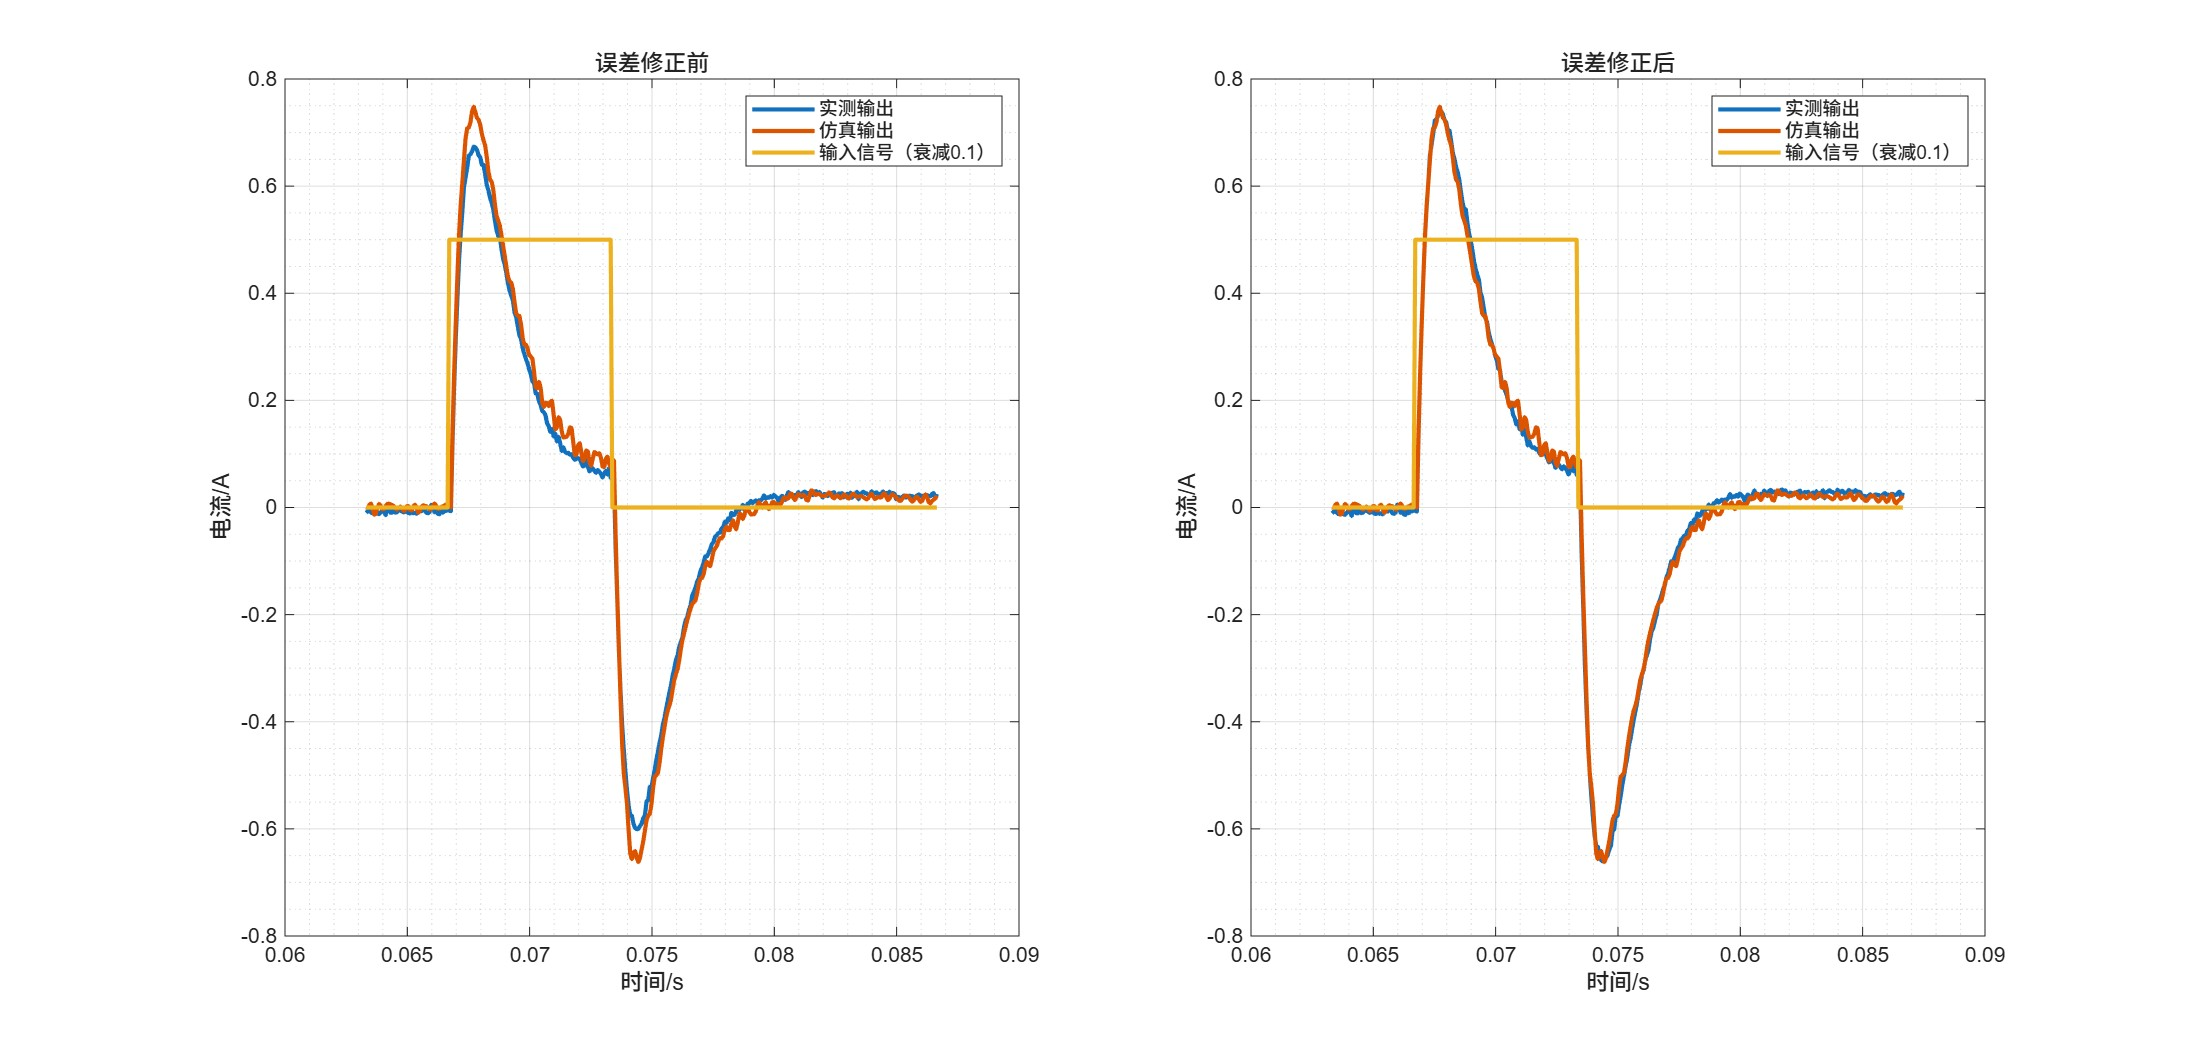
\includegraphics[width=\textwidth]
    {图片/Q轴模型验证（正向）.jpg}
    \caption{Q轴正向方波模型验证}
\end{figure}
\begin{figure}[H]
    \centering
    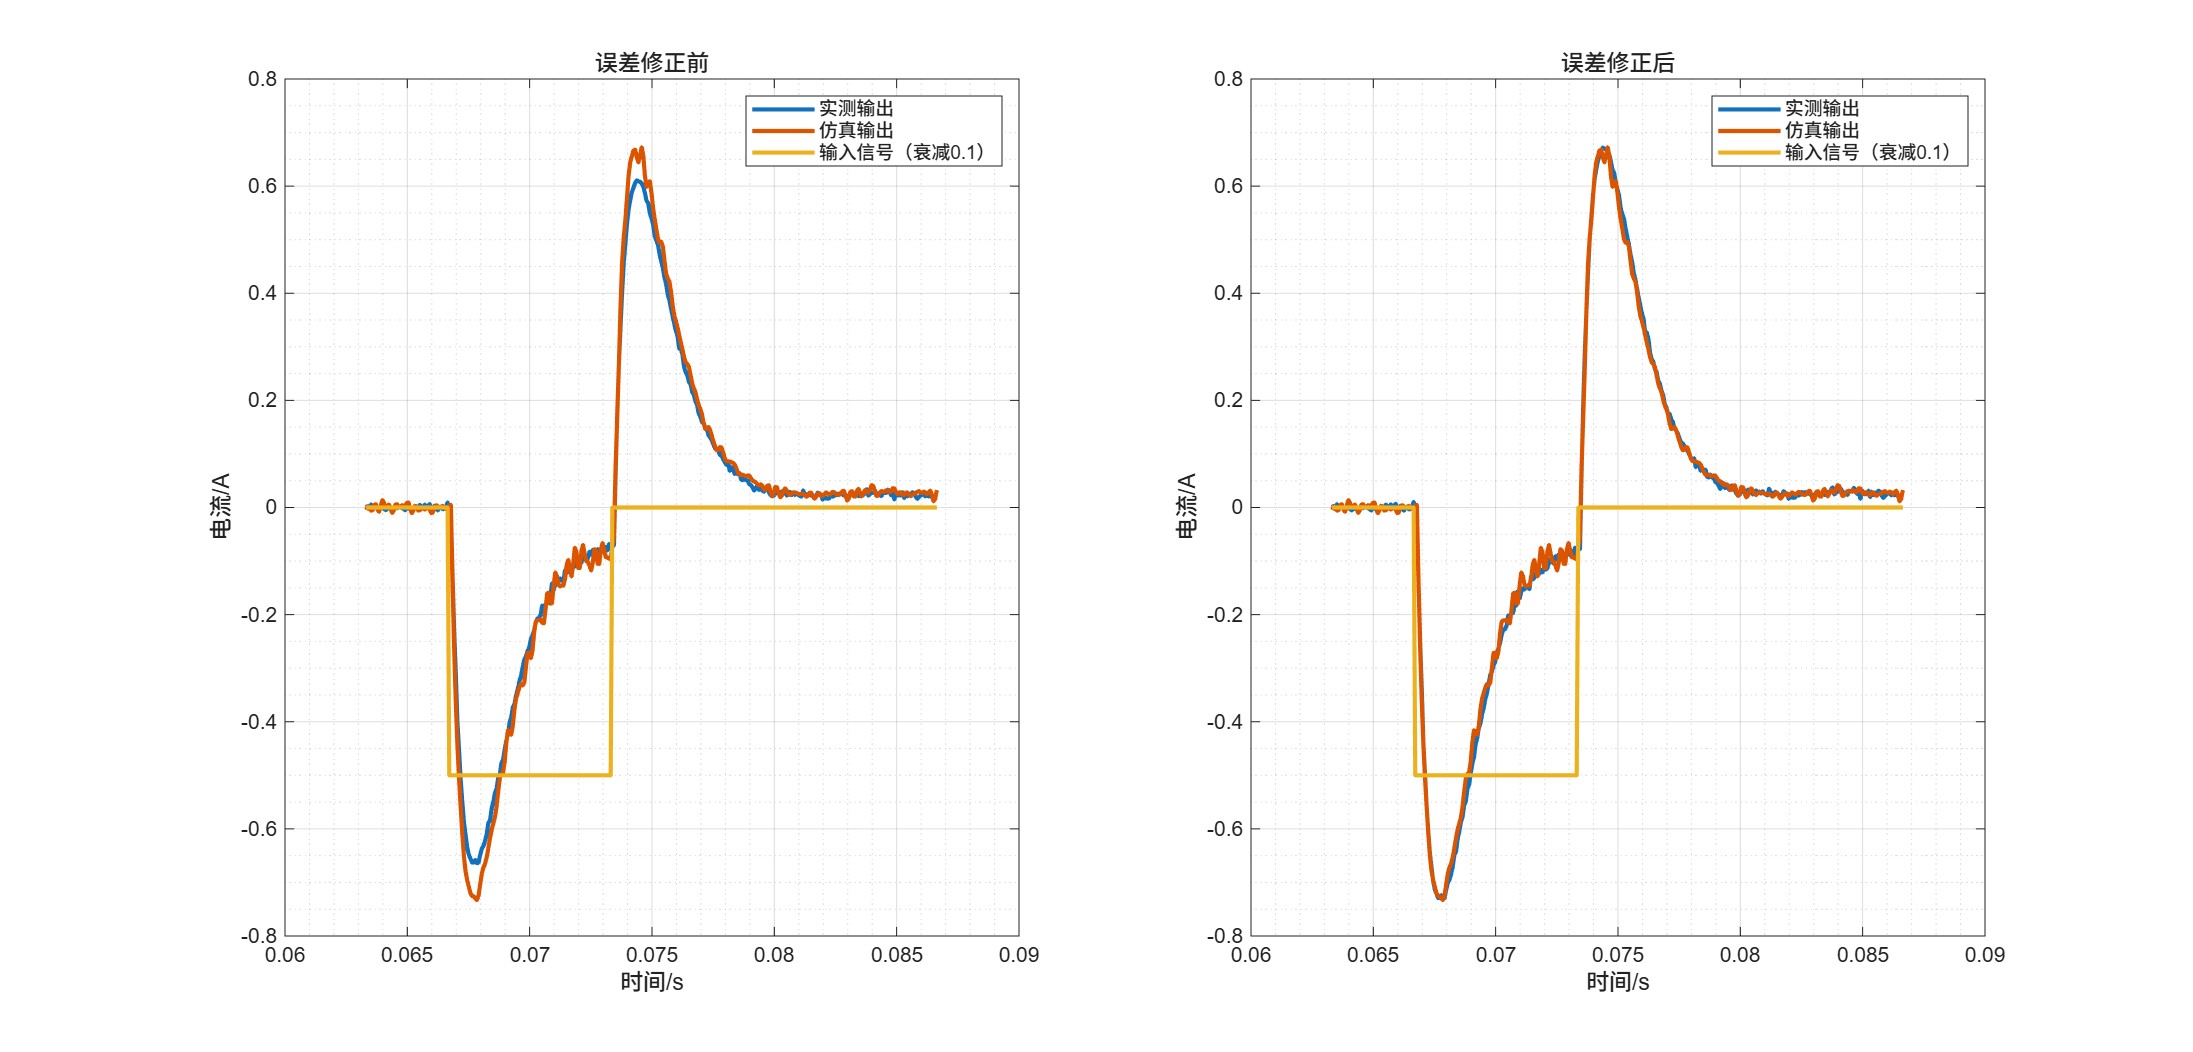
\includegraphics[width=\textwidth]
    {图片/Q轴模型验证（负向）.jpg}
    \caption{Q轴负向方波模型验证}
\end{figure}

与D轴的直流偏置加性误差不同，Q轴的实测曲线和仿真曲线之间存在增益偏差，属于乘性误差。
该误差的成因比D轴的加性误差成因更为复杂。D轴的等效RL电路模型无需反电动势补偿
（测试时保持\(i_q\approx 0\)即无交叉耦合），误差仅来源于电流采样链路的固定偏置。
而Q轴在空载测试时电机会因电磁转矩而转动，必须按
\(U_q'=U_q-\omega_e(L_d i_d+\psi_m)\)补偿反电动势才能将Q轴等效为RL电路。该补偿环节引入了
三个额外的误差源：
\begin{itemize}
    \item 永磁磁链\(\psi_m\)的辨识值存在误差，且\(\psi_m\)随温度升高而降低，实际运行中
    难以实时校准；
    \item 电角速度\(\omega_e\)的测量存在量化噪声和相位延迟，在方波跳变沿附近转速突变
    时尤为显著；
    \item 上述两项误差经乘积\(\omega_e\psi_m\)放大后注入等效电压\(U_q'\)，误差大小与
    转速成正比，而转速又与激励电流幅值正相关，因此误差呈现与信号幅值成比例的乘性特征。
\end{itemize}
一种简单的修正方法是对实测曲线施加一个缩放因子k，使得修正后两条曲线的峰值一致。误差修正前后的拟合程度如下表所示
\footnote{与加性误差同理，乘性误差修正前后相关系数保持不变（线性变换不改变线性相关程度），
而拟合优度因消除了增益偏差而升高。}。

\begin{table}[H]
    \centering
    \begin{tabular}{|c|c|c|c|c|}
        \hline
        \multirow{2}{*}{} & \multicolumn{2}{c|}{误差修正前} & \multicolumn{2}{c|}{误差修正后} \\
        \cline{2-5}
        & 相关系数 & 拟合优度 & 相关系数 & 拟合优度 \\
        \hline
        Q轴正向 & 99.86998\(\%\) & 90.06071\(\%\) & 99.86998\(\%\) & 94.71557\(\%\) \\
        \hline
        Q轴负向 & 99.91898\(\%\) & 91.09869\(\%\) & 99.91898\(\%\) & 95.53193\(\%\) \\
        \hline
    \end{tabular}
    \caption{Q轴开环模型验证拟合程度表}
    \label{tab:Q轴开环模型验证拟合程度表}
\end{table}

上述开环验证中，在误差修正前，无论D轴还是Q轴的拟合优度均超过90\(\%\)，
且修正后相关系数不变而拟合优度进一步提高，说明辨识模型能准确刻画电机的动态特性。
但从响应曲线也能看出，理想化DQ轴电路方程对现实电机行为的描述存在系统偏差
（D轴的加性偏置和Q轴的增益误差）。由于电流环采用带积分环节的控制器，积分作用保证了
闭环系统的稳态增益不受模型增益摄动的影响；但模型误差仍会在动态过程中影响
超调量和调节时间等暂态指标，这是后续控制器参数整定时需要关注的。

\newpage
\section{速度-电流环的频域矫正控制器设计}
\subsection{电流环的频域矫正控制器设计
\label{sec:电流环频域矫正控制器设计}}
\subsubsection{D轴频域矫正控制器设计与闭环验证}
D轴电流环的传递函数为：
\begin{align*}
    G_{\mathrm{D}}(z)&=(1-z^{-1})\mathcal{Z}[\cfrac{e^{-66.93\times10^{-6}s}}
        {s(5.70125+1.86152\times 10^{-3}s)(120\times 10^{-9}s+1)}]\\
        &=z^{-2}\cfrac{0.03222 + 0.0001666 z^{-1} + 4.22\times 10^{-21}z^{-2}}{1- 0.8154 z^{-1}}
\end{align*}

对于电流环控制，为了实现无差跟踪，需要加入积分环节\(\cfrac{1}{s}\)，使用双线性变换可得在电流环采样周期\(T_{\mathrm{s}}=66.67\)
us下的离散化形式为：
\begin{equation*}
    I(z)=\cfrac{T_{\mathrm{s}}}{2}\times\cfrac{1+z^{-1}}{1-z^{-1}}=3.332\times 10^{-5}\times\cfrac{1+z^{-1}}{1-z^{-1}}
\end{equation*}

可以构造带积分环节的等价被控对象\(I(z)G_{\mathrm{D}}(z)\)，其开环频率特性如下图所示。
\begin{figure}[H]
    \centering
    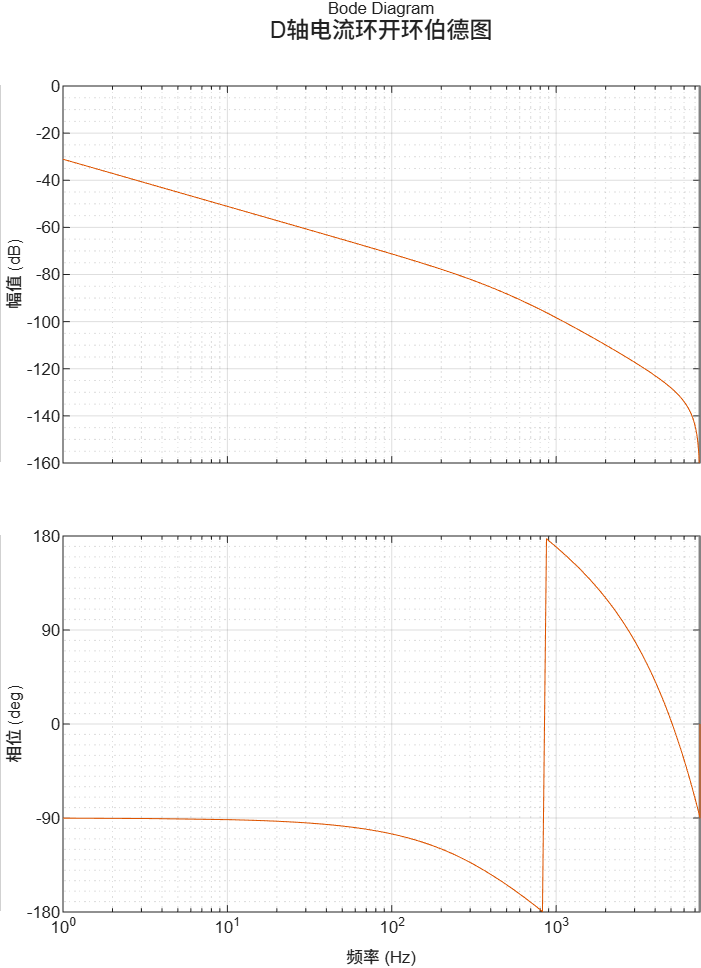
\includegraphics[width=0.5\textwidth]
    {图片/带积分环节的D轴等价被控对象开环频率特性.png}
    \caption{带积分环节的D轴等价被控对象开环频率特性}
\end{figure}

采用一阶超前校正控制\(C_{\mathrm{D}}(s)=K\cfrac{Ts+1}{\alpha Ts+1}\)，开环截止频率设定为1000Hz，以不低于40°的相位裕度为目标，
在1000Hz处提供最多60°的相位补偿，可以计算得到：
\begin{equation*}
    \begin{cases}
        \alpha = \cfrac{1-\sin(60°)}{1+\sin(60°)}=0.0718\\
        T = \cfrac{1}{2\pi\times 1000\sqrt{\alpha}} = 5.9391\times 10^{-4}
    \end{cases}
\end{equation*}

最后根据等价被控对象在1000Hz处的增益，调整放大系数K，最终可得带积分的D轴超前控制器：
\begin{equation*}
    C_{\mathrm{D}}(s)=\cfrac{12.95s+2.18\times 10^4}{4.265\times 10^{-5}s^2+s}
\end{equation*}

使用双线性变换离散化后得到\footnote{对于采用双线性变换离散化的控制器，积分环节对应为z=1的极点。因此要求离散后分母各个系数之和
要严格为零，否则z=1处的极点就会发生偏移，积分环节变为惯性环节。在正常工况下影响不大，但是在极端情况（如长时间堵转、积分严重
饱和）会导致系统行为失常。MATLAB默认显示四位有效数字，可能会导致精度损失，此时需要手动点开传递函数数据结构查看
更精确的值}：
\begin{equation*}
    C_{\mathrm{D}}(z)=\cfrac{5.998+0.6373z^{-1}-5.361z^{-2}}{1-1.1227z^{-1}+0.1227z^{-2}}
\end{equation*}

经过超前控制后的开环频率特性和闭环频率特性如下图所示。
\begin{figure}[H]
    \centering
    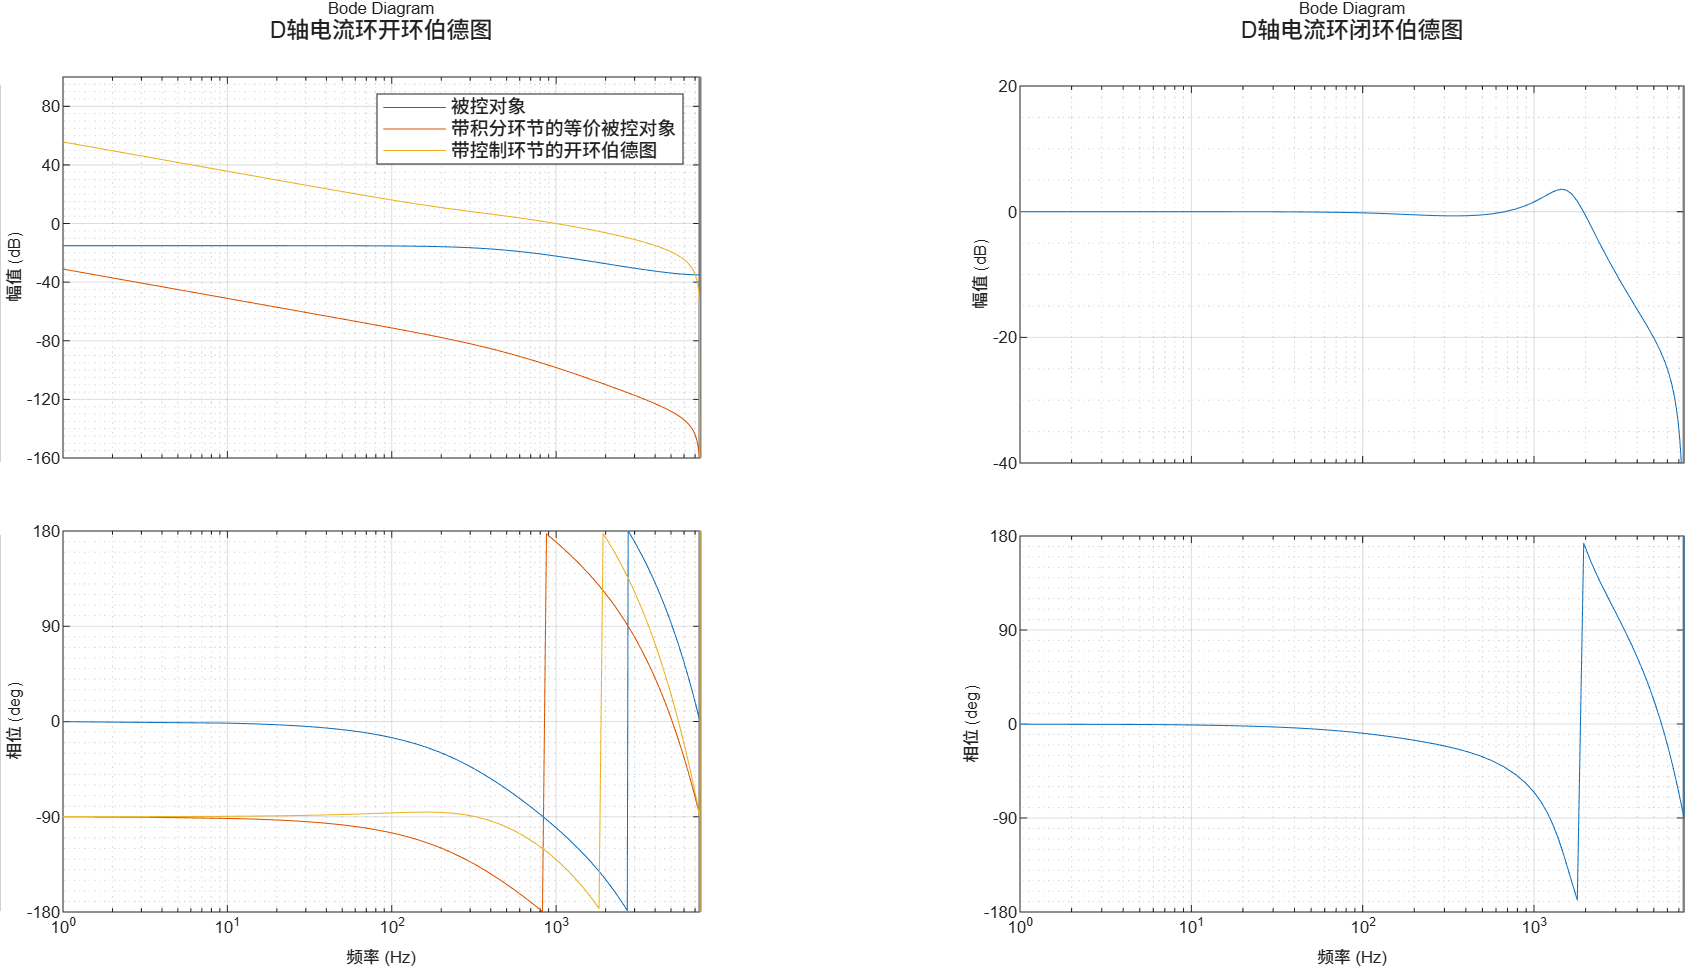
\includegraphics[width=\textwidth]
    {图片/D轴开-闭环频率特性.png}
    \caption{D轴开-闭环频率特性}
\end{figure}

矫正后，D轴电流环的开环截止频率1000.00073Hz，相位裕度49.46547°满足设计要求。相位穿越频率1883.94275Hz，
幅值裕度5.69334dB，闭环带宽2213.62137Hz。闭环前后的单位阶跃响应如下图所示。
\begin{figure}[H]
    \centering
    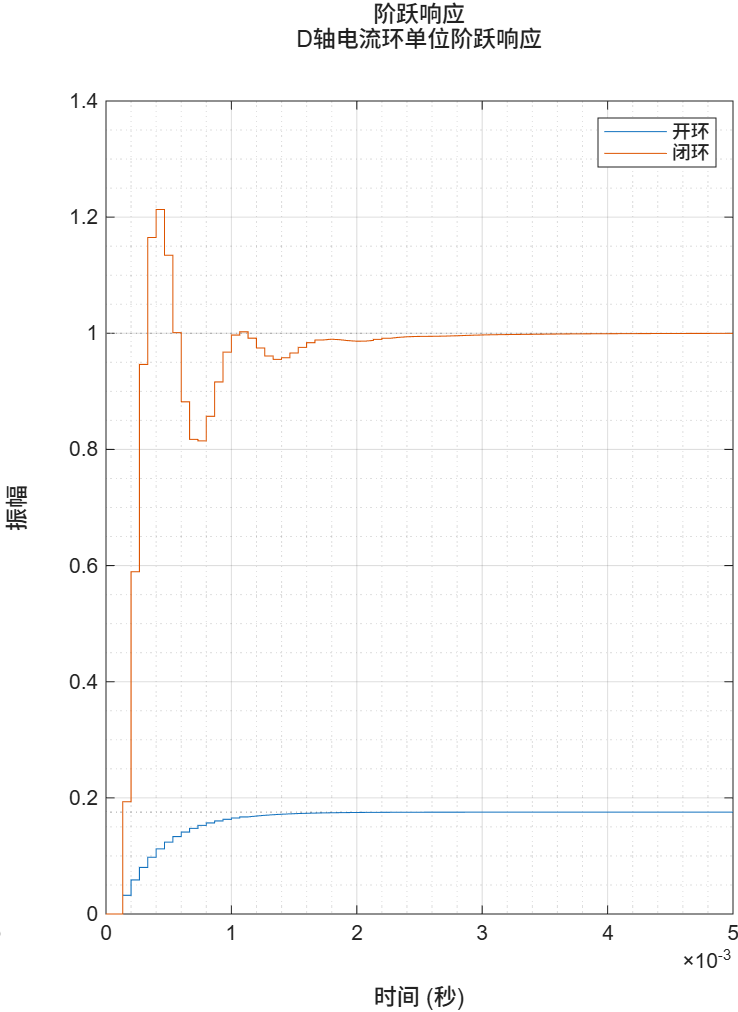
\includegraphics[width=0.5\textwidth]
    {图片/D轴开-闭环单位阶跃响应对比.png}
    \caption{D轴开-闭环单位阶跃响应对比}
\end{figure}

可以发现，通过带积分环节的超前校正控制器，使得能够无差跟踪给定信号，超调量21.3\%，调节时间为1.6ms，用一定的超调
换来了极快的响应速度。接下来考虑以±0.25A的方波电流给定信号（持续50个采样周期）进行测试，以评估实际系统响应和
建模准确性，结果如下图所示。
\begin{figure}[H]
    \begin{minipage}{0.5\textwidth}
        \centering
        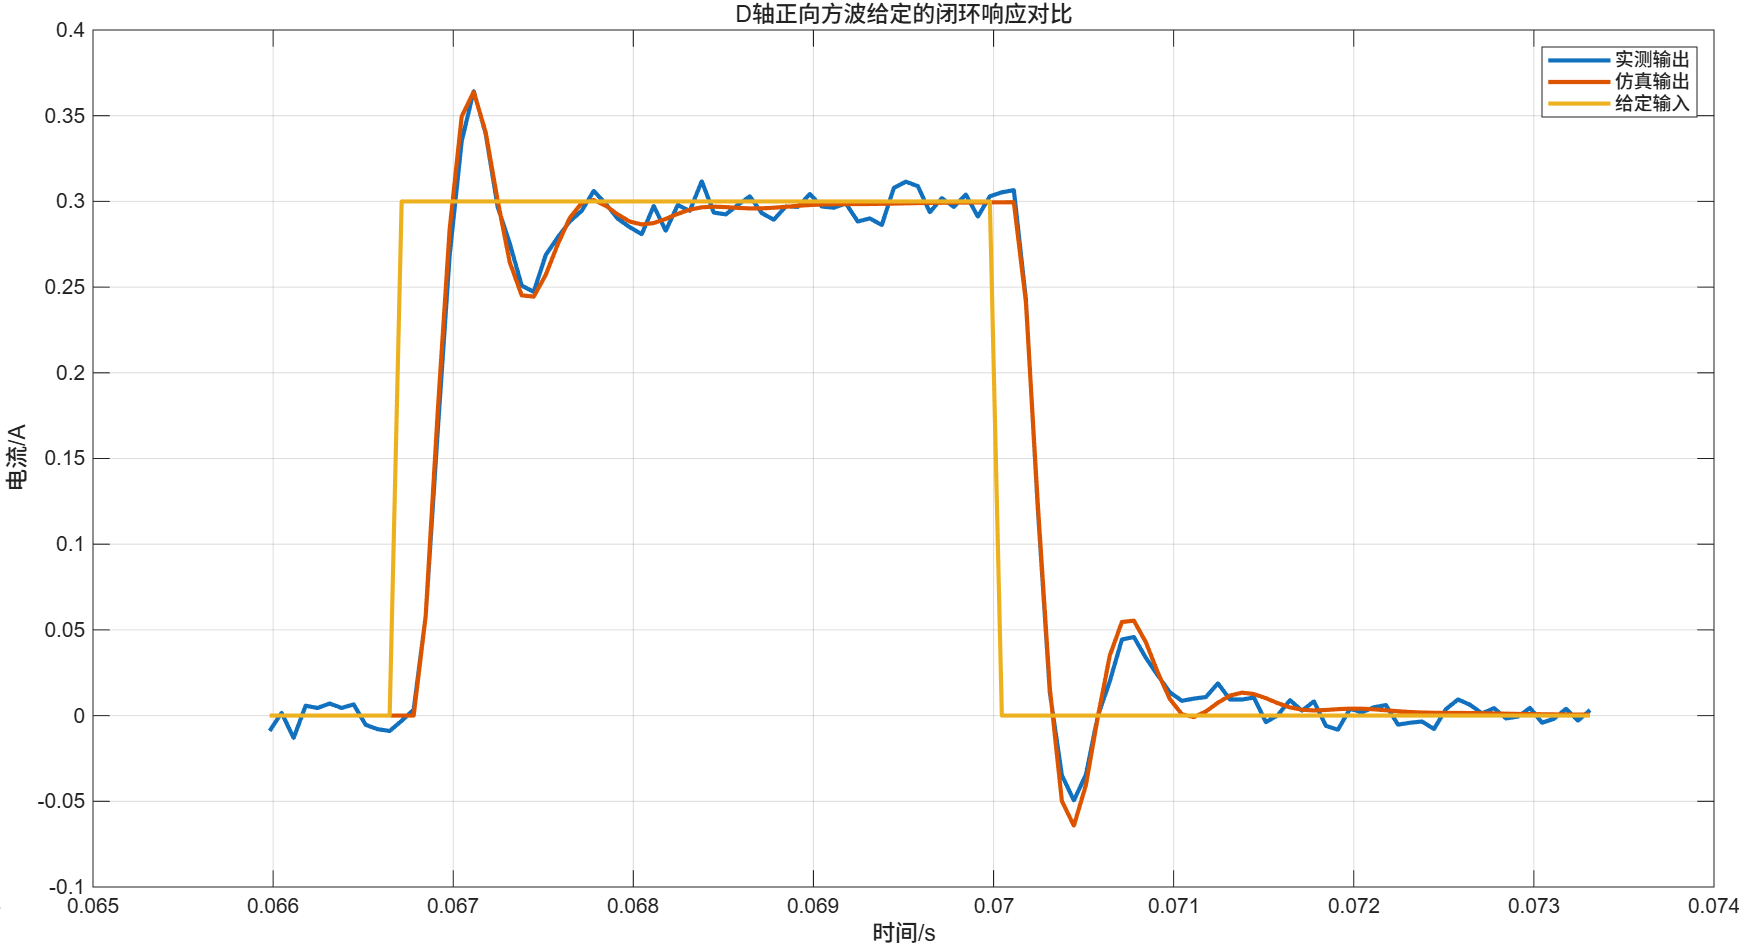
\includegraphics[width=\textwidth]
        {图片/D轴正向方波闭环验证.png}
        \caption{D轴正向方波闭环验证}
    \end{minipage}
    \begin{minipage}{0.5\textwidth}
        \centering
        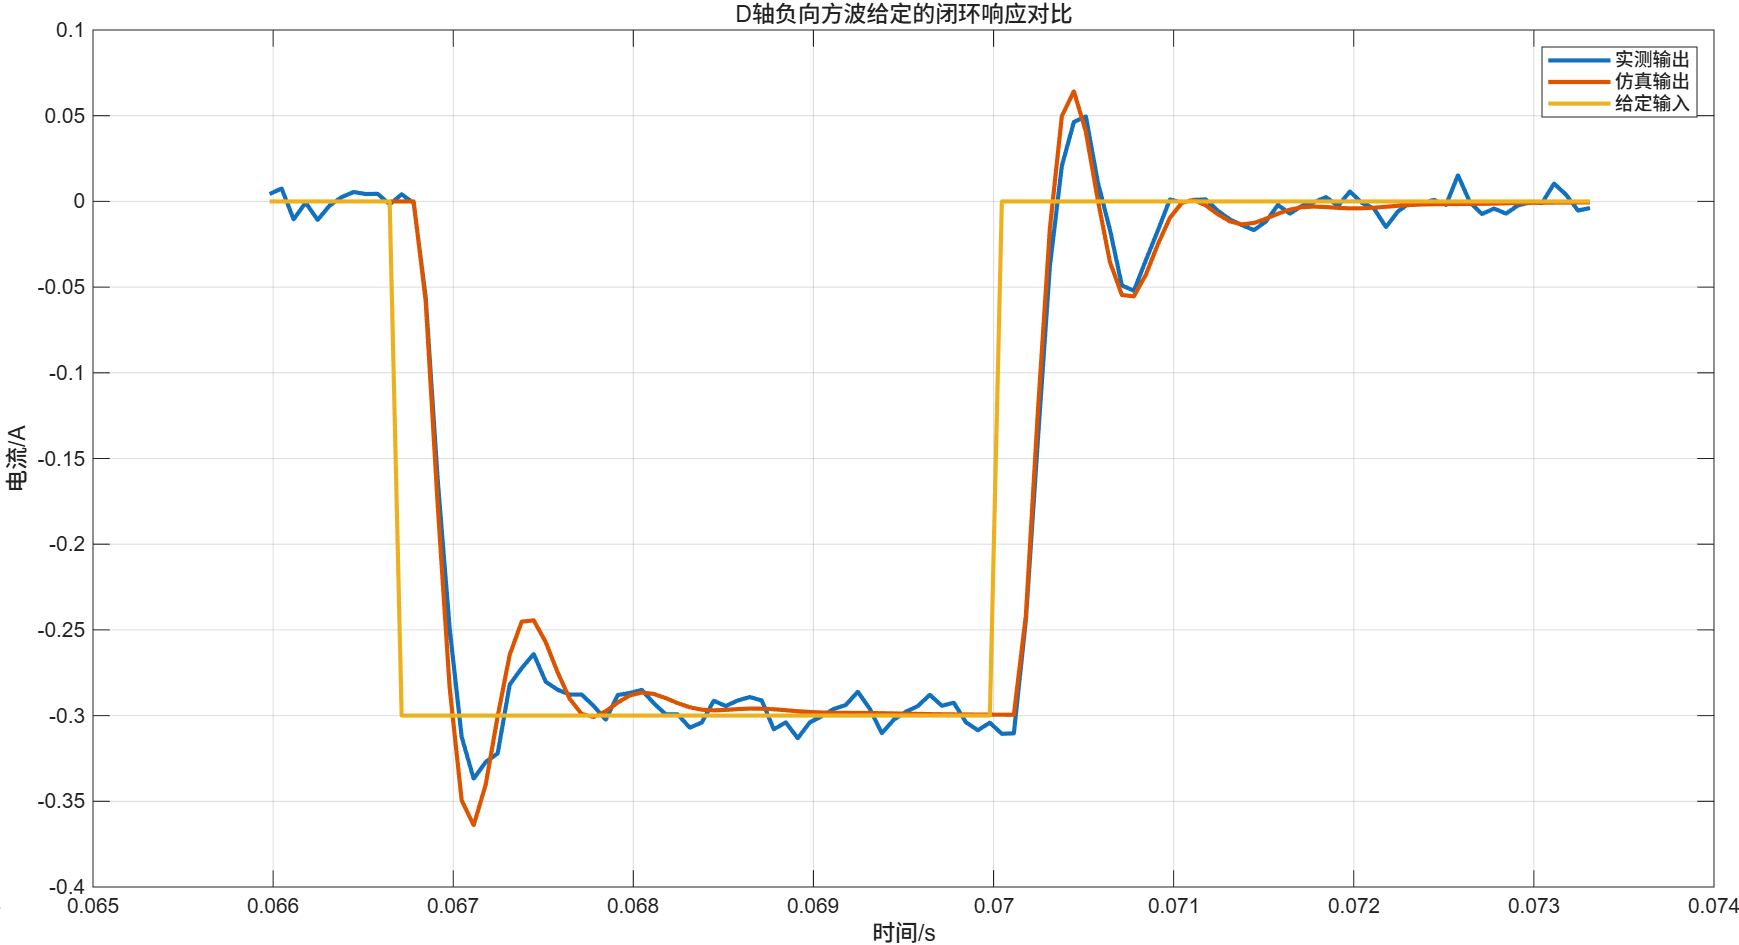
\includegraphics[width=\textwidth]
        {图片/D轴负向方波闭环验证.png}
        \caption{D轴负向方波闭环验证}   
    \end{minipage}
\end{figure}

据上图可知，由于存在采样噪声且进行闭环控制后系统对采样噪声的敏感度升高，导致实测电流波形有较大的波动。但在
整体趋势上和仿真波形一致。
正向方波中相关系数为99.88301\%，拟合优度95.15871\%；
负向方波中相关系数为99.73266\%，拟合优度92.69211\%，均为较高水平。

\subsubsection{Q轴频域矫正控制器设计与闭环验证}
Q轴电流环的传递函数为：
\begin{align*}
    G_{\mathrm{Q}}(z)&=(1-z^{-1})\mathcal{Z}[\cfrac{e^{-66.93\times10^{-6}s}}
        {s(5.70125+2.16828\times 10^{-3}s)(120\times 10^{-9}s+1)}]\\
        &=z^{-2}\cfrac{0.02805 + 0.0001482 z^{-1}+5.776\times 10^{-21}z^{-2}}{1- 0.8393 z^{-1}}
\end{align*}

与D轴同理，在电流环中串联积分环节\(I(z)\)以消除稳态误差，构造带积分环节的等价被控对象
\(I(z)G_{\mathrm{Q}}(z)\)，其开环频率特性如下图所示。
\begin{figure}[H]
    \centering
    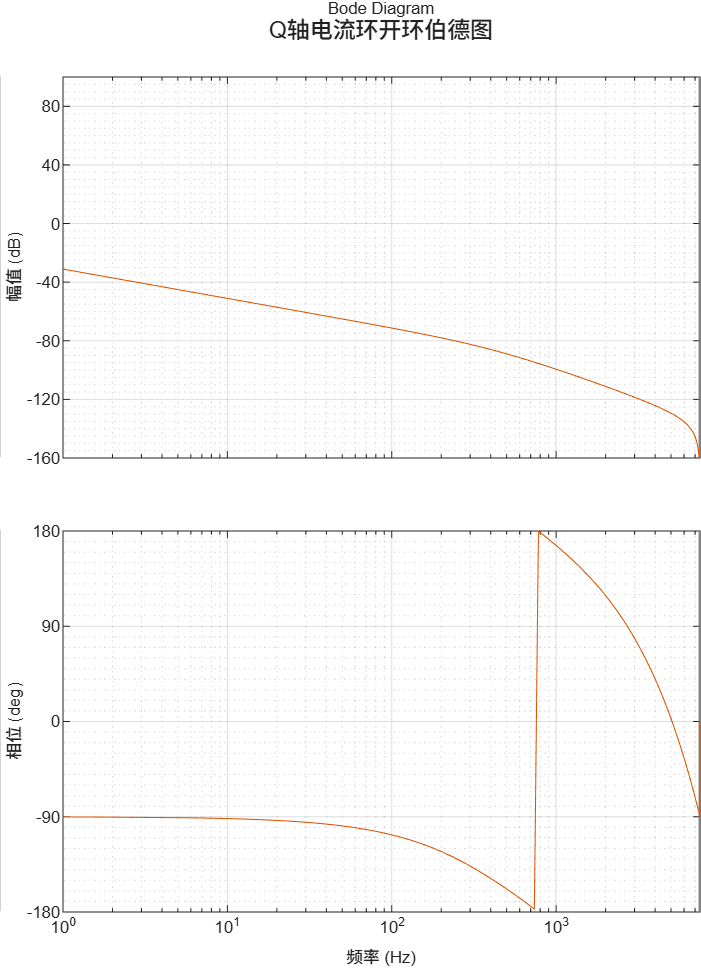
\includegraphics[width=0.5\textwidth]
    {图片/带积分环节的Q轴等价被控对象开环频率特性.png}
    \caption{带积分环节的Q轴等价被控对象开环频率特性}
\end{figure}

采用与D轴相同的一阶超前校正结构\(C_{\mathrm{Q}}(s)=K\cfrac{Ts+1}{\alpha Ts+1}\)，设计指标保持一致：
开环截止频率1000Hz，相位裕度不低于40°，在1000Hz处提供最多60°的相位补偿。\(\alpha\)和\(T\)
的取值与D轴完全相同（\(\alpha=0.0718\)，\(T=5.9391\times 10^{-4}\)），仅需根据Q轴等价被控对象
在1000Hz处的增益调整放大系数\(K\)。由于Q轴电感大于D轴（\(L_{\mathrm{q}}=2.16828\textrm{mH}>L_{\mathrm{d}}=1.86152\textrm{mH}\)），
Q轴RL电路的转折频率更低，1000Hz处的增益衰减更大，因此需要略高的\(K\)值补偿。最终可得带积分的
Q轴超前控制器：
\begin{equation*}
    C_{\mathrm{Q}}(s)=\cfrac{14.7s+2.474\times 10^4}{4.265\times 10^{-5}s^2+s}
\end{equation*}

使用双线性变换离散化后得到：
\begin{equation*}
    C_{\mathrm{Q}}(z)=\cfrac{6.808+0.7233z^{-1}-6.085z^{-2}}{1-1.1227z^{-1}+0.1227z^{-2}}
\end{equation*}

经过超前控制后的开环频率特性和闭环频率特性如下图所示。
\begin{figure}[H]
    \centering
    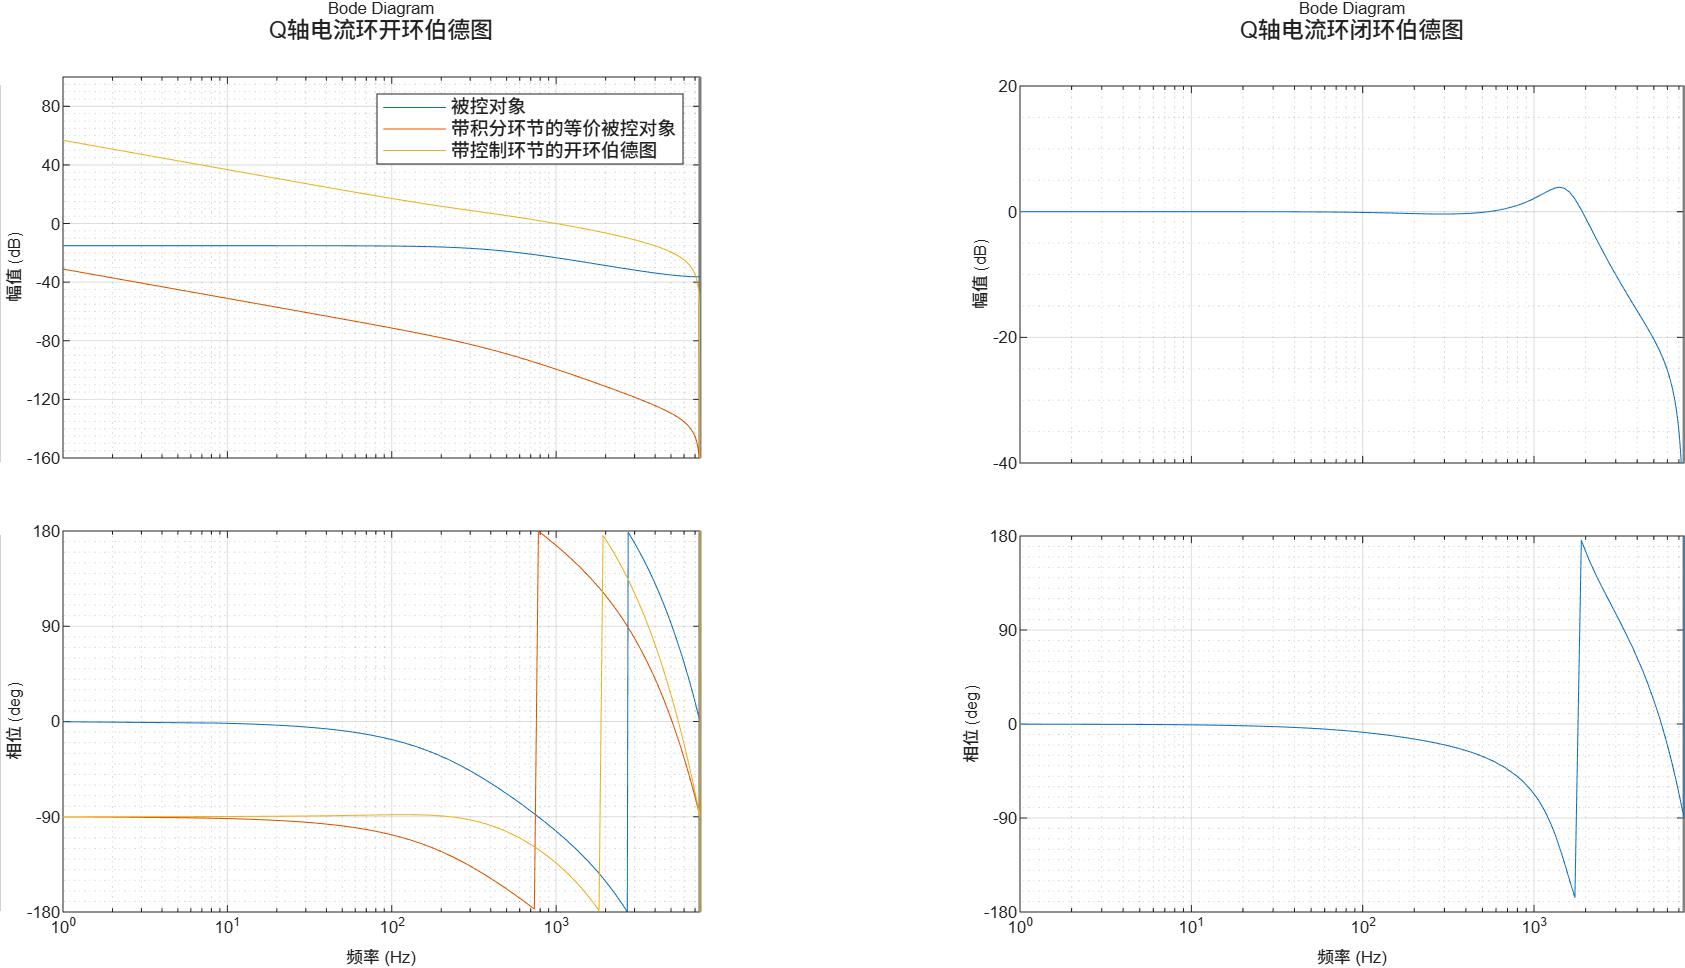
\includegraphics[width=\textwidth]
    {图片/Q轴开-闭环频率特性.png}
    \caption{Q轴开-闭环频率特性}
\end{figure}

矫正后，Q轴电流环的开环截止频率1000.00063Hz，相位裕度46.24331°满足设计要求。
相位穿越频率1848.20511Hz，幅值裕度5.65228dB，闭环带宽2179.71785Hz。
闭环前后的单位阶跃响应如下图所示。
\begin{figure}[H]
    \centering
    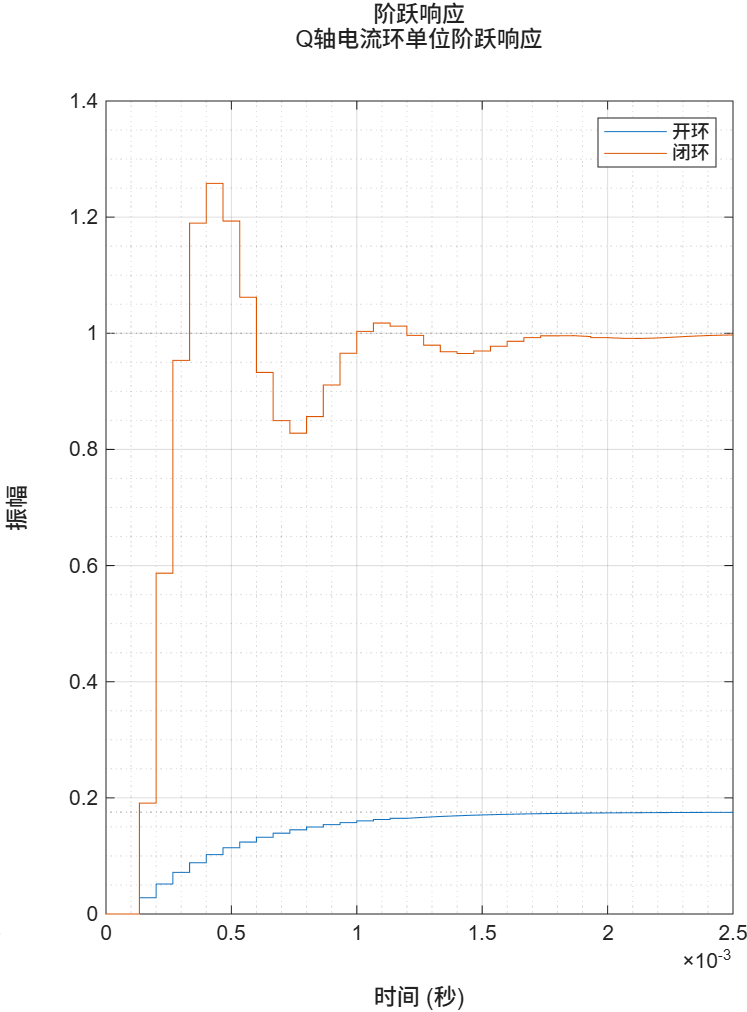
\includegraphics[width=0.5\textwidth]
    {图片/Q轴开-闭环单位阶跃响应对比.png}
    \caption{Q轴开-闭环单位阶跃响应对比}
\end{figure}

可以发现，Q轴闭环阶跃响应的超调量25.8\%，调节时间1.6ms，与D轴基本一致，这是因为
两者采用了相同的频域设计指标和校正器结构。

接下来以±0.25A的方波电流给定信号进行闭环跟踪测试。与D轴方波持续50个采样周期不同，
Q轴的方波仅持续5个采样周期\footnote{Q轴测试时电机会因电磁转矩而转动，方波持续时间过长将导致
转速累积升高，反电动势\(\omega_{\mathrm{e}}(\psi_{\mathrm{m}}+L_{\mathrm{d}}i_{\mathrm{d}})\)随之增大，削弱等效Q轴电压\(U_{\mathrm{q}}'\)中的激励分量，
迫使控制器持续增大\(U_{\mathrm{q}}\)以维持跟踪，最终进入饱和区，使系统非线性显著增强而难以进行线性仿真分析。
缩短方波持续时间可限制电机转角与转速的累积，将反电动势对等效RL电路模型的干扰控制在可忽略范围内。}。
闭环验证结果如下图所示。
\begin{figure}[H]
    \begin{minipage}{0.5\textwidth}
        \centering
        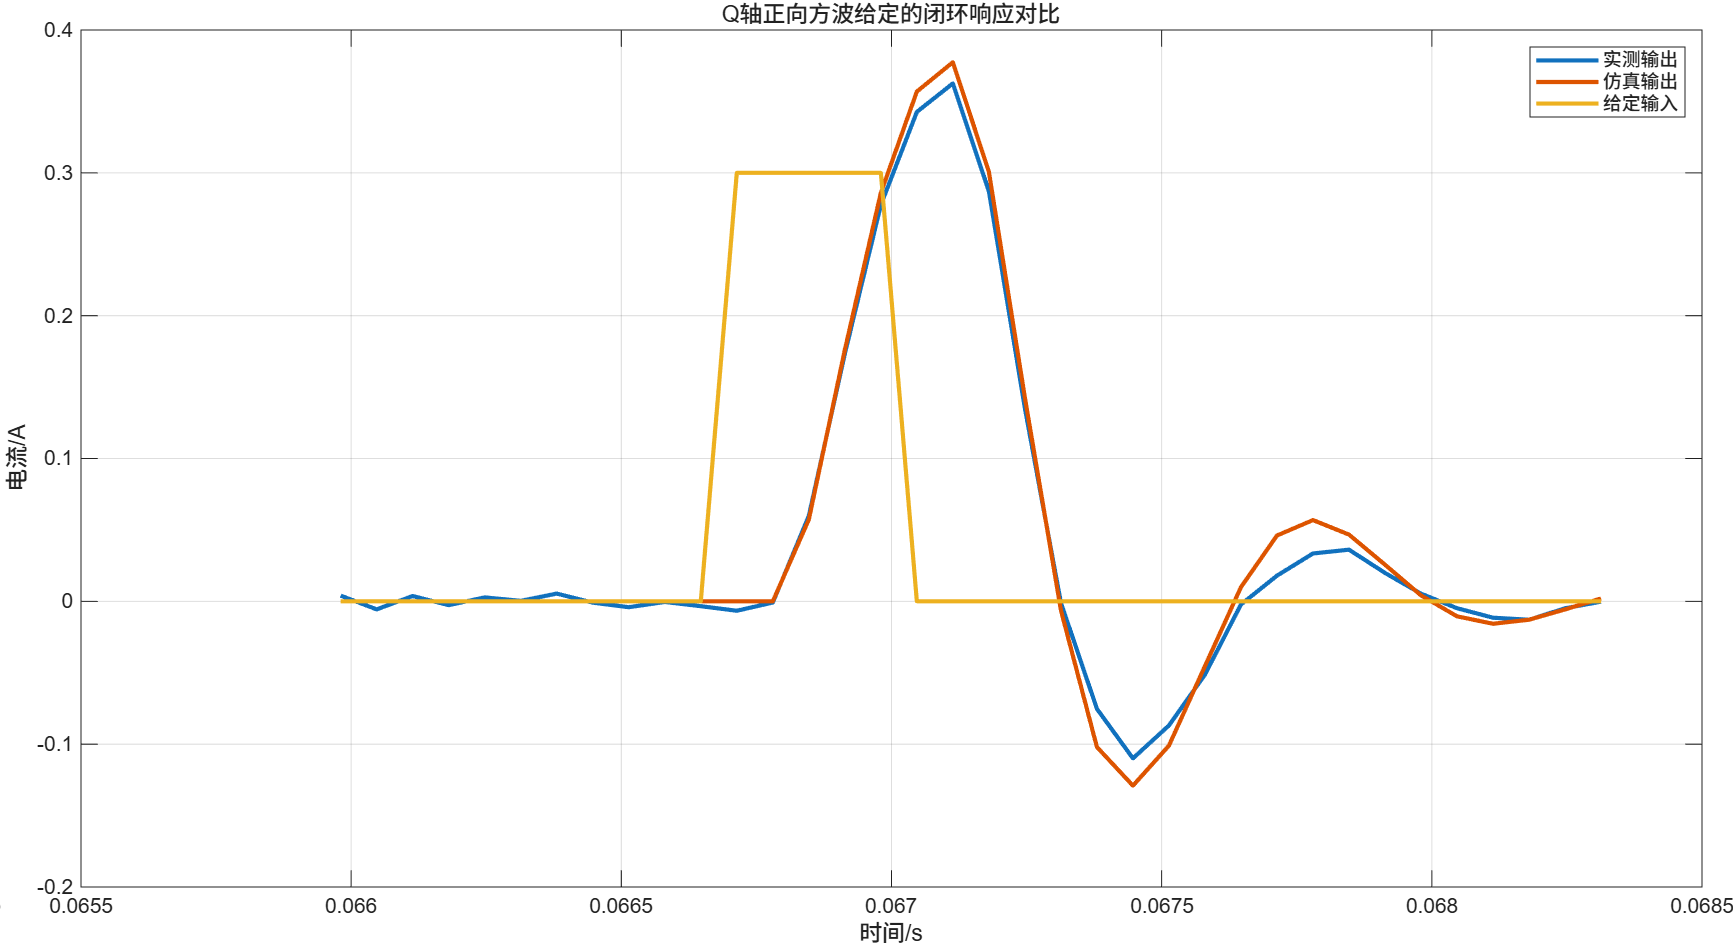
\includegraphics[width=\textwidth]
        {图片/Q轴正向方波闭环验证.png}
        \caption{Q轴正向方波闭环验证}
    \end{minipage}
    \begin{minipage}{0.5\textwidth}
        \centering
        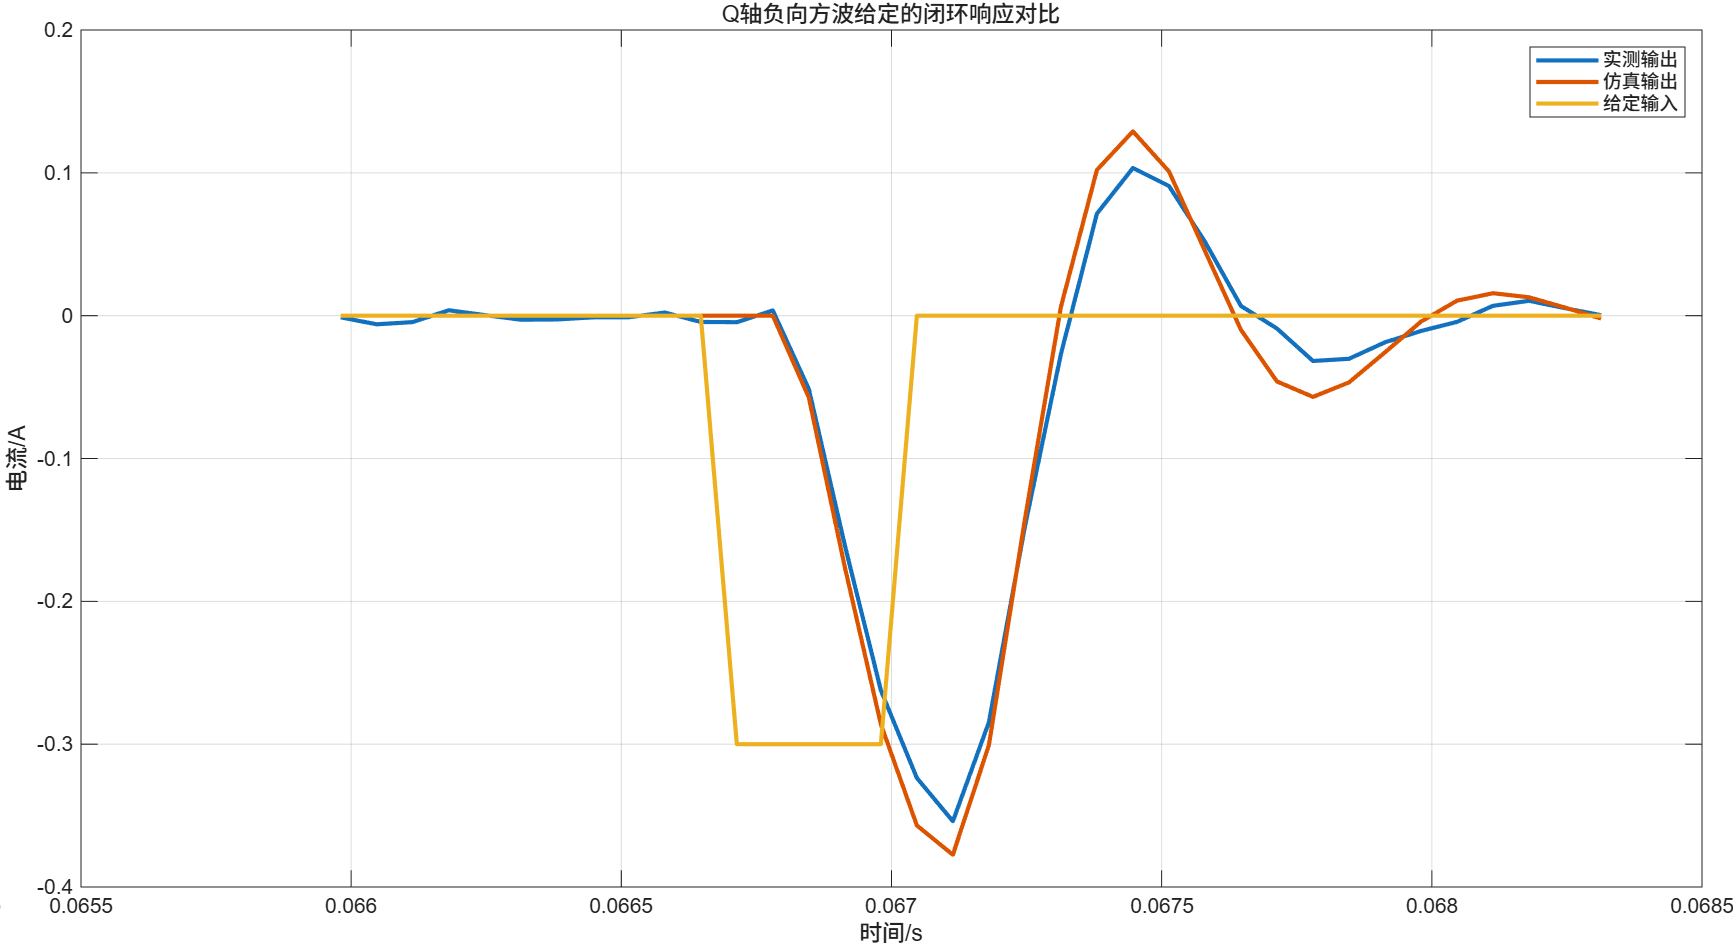
\includegraphics[width=\textwidth]
        {图片/Q轴负向方波闭环验证.png}
        \caption{Q轴负向方波闭环验证}
    \end{minipage}
\end{figure}

由于Q轴方波持续时间极短（5个采样周期仅约0.33ms），远小于闭环调节时间（1.6ms），
电流在每个脉冲内尚未到达稳态即被翻转，因此该测试实质上是暂态跟踪能力的验证，
而非稳态方波跟踪。实测曲线与仿真曲线的趋势吻合良好，
正向方波中相关系数为99.71872\%，拟合优度90.50733\%；
负向方波中相关系数为99.42643\%，拟合优度85.36039\%，
验证了Q轴频域校正控制器的瞬态响应有效性。

\subsection{速度环辨识理论分析}
虽然前文已经完成了Q轴电流环的闭环校正，但在速度环辨识中并未直接以电流给定\(i_{\mathrm{q}}^*\)作为激励
输入。其原因是Q轴电流控制器\(C_{\mathrm{Q}}(z)\)中含有积分环节，若以\(i_{\mathrm{q}}^*\)
\footnote{用上标*表示对某个物理量的给定/期望（如\(i_{\mathrm{d}}^*,i_{\mathrm{q}}^*,n^*\)），无上标*的表示实际值
（如\(i_{\mathrm{d}},i_{\mathrm{q}},n\)）。}
替代\(U_{\mathrm{q}}\)作为输入，辨识过程中积分器将持续累积\(i_{\mathrm{q}}^*\)与实际\(i_{\mathrm{q}}\)之间的跟踪误差并迅速
进入饱和区，使系统非线性显著增强，违背线性辨识的基本假设。因此，速度环的辨识仍以\(U_{\mathrm{q}}\)作为可操作变量。

速度环辨识的对象是机械部分的传递函数\(G_{\mathrm{m}}(s)\)，即从电磁转矩\(T_{\mathrm{e}}\)到转速\(n\)的传递函数。
由于电磁转矩无法直接测量，只能由实测电流重构。此外，反电动势\(\omega_{\mathrm{e}}\psi_{\mathrm{m}}\)构成物理闭环，
使得对该传递函数的直接辨识必然在闭环条件下进行，存在理论上的偏倚。

在空载情况下，电机的机械部分一般被建模为带有与速度成正比的粘滞摩擦环节，即一般认为传递函数为：
\begin{equation*}
    G_{\mathrm{m}}(s)=\cfrac{n(s)}{T_{\mathrm{e}}(s)}=\cfrac{1}{B+Js}
\end{equation*}

但是由于电机的机械部分非线性因素远超电气部分，上述假设在实际中往往无法成立分析。因此在这里将机械部分视为一个
阶次不定的系统，在特定工作点附近的局部线性化传递函数为\(G_{\mathrm{m}}(s)\)

在\(i_{\mathrm{d}}^*=0\)的条件下，\(U_{\mathrm{d}}\)用于维持理想化的\(i_{\mathrm{d}}=0\)条件，而\(U_{\mathrm{q}}\)用于控制\(i_{\mathrm{q}}\)，实现转矩环和速度环控制。
此时电磁转矩为\(T_{\mathrm{e}}=\cfrac{3}{2}p\psi_{\mathrm{m}}i_{\mathrm{q}}\propto i_{\mathrm{q}}\)为线性增益环节。而Q轴反电动势为
\(E=\omega_{\mathrm{e}}(\psi_{\mathrm{m}}+L_{\mathrm{d}}i_{\mathrm{d}})\)，在\(i_{\mathrm{d}}=0\)时可以简化为\(E=\omega_{\mathrm{e}}\psi_{\mathrm{m}}\propto \omega_{\mathrm{e}}\)也是线性增益环节。
考虑电角速度\(\omega_{\mathrm{e}}\)与转速\(n\)满足\(\omega_{\mathrm{e}}=\cfrac{\pi}{30}np\)，因此反电动势可以表示为
\(E=\cfrac{\pi}{30}np\psi_{\mathrm{m}}\propto n\)。

因此可以得到从\(U_{\mathrm{q}}\)到\(n\)在\(i_{\mathrm{d}}=0\)的理想化假设下系统框图：
\begin{figure}[H]
    \centering
    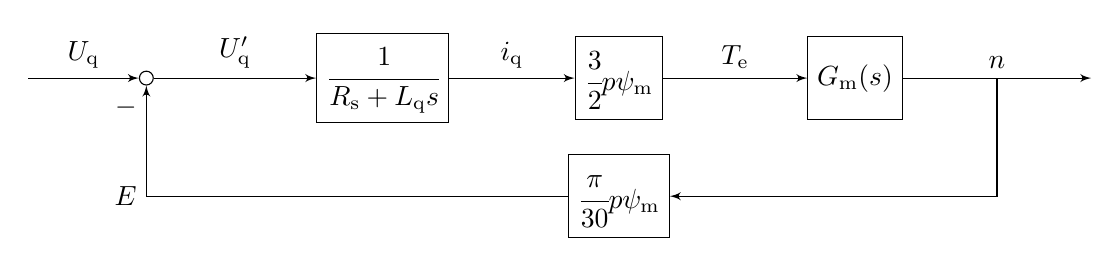
\begin{tikzpicture}[auto, node distance=3cm, >=latex']
        % 样式定义
        \tikzstyle{block} = [draw, rectangle, minimum height=3em, minimum width=3em, align=center]
        \tikzstyle{sum} = [draw, circle, node distance=1.5cm, minimum size=0.5em, inner sep=0pt]
        \tikzstyle{input} = [coordinate]
        \tikzstyle{output} = [coordinate]
        \tikzstyle{feedback} = [coordinate]

        % 放置节点
        \node [input, name=input] {};
        \node [sum, right of=input] (sum) {};
        \node [block, right of=sum] (RL) {\(\cfrac{1}{R_{\mathrm{s}}+L_{\mathrm{q}} s}\)};
        \node [block, right of=RL] (K) {\(\cfrac{3}{2}p\psi_{\mathrm{m}}\)};
        \node [block, right of=K] (Mech) {\(G_{\mathrm{m}}(s)\)};
        \node [output, right of=Mech] (output) {};
        \node [block, below of=K, node distance=1.5cm] (Kf) {\(\cfrac{\pi}{30}p\psi_{\mathrm{m}}\)};

        \draw [->] (input) -- node {\(U_{\mathrm{q}}\)} (sum);
        \draw [->] (sum) -- node {\(U_{\mathrm{q}}'\)} (RL);
        \draw [->] (RL) -- node {\(i_{\mathrm{q}}\)} (K);
        \draw [->] (K) -- node {\(T_{\mathrm{e}}\)} (Mech);
        \draw [->] (Mech) -- node [name=y] {\(n\)} (output);
        \draw [->] (y) |- (Kf);
        \draw [->] (Kf) -| node[pos=0.9] {\(-\)} node [pos=0.5] {\(E\)} (sum);
    \end{tikzpicture}
    \caption{\(i_{\mathrm{d}}=0\)假设下的Q轴电流-速度系统框图}
    \label{fig:Q轴电流-速度系统框图}
\end{figure}

按照先前直接辨识的思路，以\(U_{\mathrm{q}}\)为可操作输入量，测量\(T_{\mathrm{e}}\)视为实际输入，\(n\)为输出量，辨识
从\(T_{\mathrm{e}}\)到\(n\)的传递函数。设存在理想测量白噪声\(n_{\mathrm{T}}\)和
\(n_{\mathrm{n}}\)，无噪声的理论值为\(T_{0}\)和\(n_0\)。Ho-Kalman算法利用维纳-霍普夫方程估计系统的脉冲响应进行辨识，可以得到：
\begin{align*}
    n_k&=n_{0,k}+n_{\mathrm{n},k}\\
    &=T_0*g_{\mathrm{m}}+n_{\mathrm{n},k}\\
    &=(T_k-n_{\mathrm{T},k})*g_{\mathrm{m}}+n_{\mathrm{n},k}\\
    &=T_k*g_{\mathrm{m}}-n_{\mathrm{T},k}*g_{\mathrm{m}}+n_{\mathrm{n},k}
\end{align*}

对上式进行自相关运算，求解输入自功率谱密度函数和输入输出互功率谱密度函数，其商就是估计脉冲响应的离散傅里叶变换DTFT：
\begin{equation*}
    \hat{G}_{\mathrm{m}}(e^{\mathrm{j}\omega})=G_{\mathrm{m}}(e^{\mathrm{j}\omega})
    [1-\cfrac{\sigma_{\mathrm{T}}^2}{S_{T_{\mathrm{e}}T_{\mathrm{e}}}(e^{\mathrm{j}\omega})}]
\end{equation*}

其中\(\sigma_{\mathrm{T}}^2\)为测量噪声\(n_{\mathrm{T}}\)的方差，而\(S_{T_{\mathrm{e}}T_{\mathrm{e}}}(e^{\mathrm{j}\omega})\)
为实际测量值的自功率谱密度函数。由上式可知，在闭环情况下，
试图用开环的算法估计系统的脉冲响应，进而去分析系统的传递函数，结果将是有偏的。

需要注意的是，数学上有偏并不代表工程上不可行。若偏差很小，不影响工程分析，那么即使理论有偏在工程上也是可以接受的。如根据
图\ref{fig:Q轴电流-速度系统框图}，在\ref{sec:Q轴同步电感辨识}中进行的Q轴同步电感辨识方法也将是有偏的
\footnote{具体推导见\ref{sec:偏差直接重构中间到中间/输出的偏倚性分析}。}，但在开环和闭环验证中
均证实了辨识结果的有效性。因此，需要相干函数评估辨识结果的工程可用性：
\begin{equation}
    \gamma_{xy}^2(\omega)=\frac{|S_{xy}(e^{\mathrm{j}\omega})|^2}{S_{xx}(e^{\mathrm{j}\omega})\,S_{yy}(e^{\mathrm{j}\omega})}
    \label{eq:相干函数定义}
\end{equation}

其中\(S_{xy}(e^{\mathrm{j}\omega})\)为互功率谱密度，\(S_{xx}(e^{\mathrm{j}\omega})\)和\(S_{yy}(e^{\mathrm{j}\omega})\)为自功率谱密度。
相干函数满足\(0\le \gamma_{xy}^2(\omega)\le 1\)，在某个频点的值越接近1，说明输出信号中该频点的分量可以被输入信号线性解释的比例越高，
使用维纳-霍普夫方程估计脉冲响应序列在这个频点的可信度也越高。相干函数作为信噪比度量的含义、与偏置因子之间的联系详见\ref{sec:相干函数与估计质量的评估}。

为对比不同辨识策略在反电动势造成的闭环结构下的表现，考虑四种候选的待辨识传递函数，并分别计算其相干函数。这四种待辨识传递函数取自同一物理系统
（FOC控制下的永磁同步电机），覆盖了辨识问题中可能的输入输出选取方式，并在以下维度上彼此不同：
输入是给定还是闭环内信号、输入是直接测量还是重构、辨识工作在开环还是闭环、关注频段属于电路模态还是
机械模态。相干函数\(\gamma_{xy}^2\)经输入输出功率谱归一化，恰好可作为统一衡量这四种待辨识传递函数“输出被输入线性解释的比例”
的公共标尺。四种待辨识传递函数的差异汇总如下表所示。
\footnote{直接法辨识中选用\(i_\mathrm{q}\)而不是\(T_{\mathrm{e}}\)是因为电磁转矩无法直接测量，需要从电流中乘以常数得到，两者成正比
关系，因此分析从\(i_{\mathrm{q}}\)到\(n\)的相干函数即可。} 
\begin{table}[H]
    \centering
    \begin{tabular}{|c|c|c|c|}
        \hline
        通道 & 输入/输出 & 输入来源与结构 & 关注频段\\
        \hline
        开环基准（D轴同步电感） & \(U_{\mathrm{d}}/i_{\mathrm{d}}\) & 外部给定，开环 & 电路模态 \(100\sim3000\)Hz\\
        \hline
        重构等效输入（Q轴同步电感） & \(U_{\mathrm{q}}'/i_{\mathrm{q}}\) & 重构输入，闭环 & 电路模态 \(100\sim3000\)Hz\\
        \hline
        直接法（机械传递函数） & \(i_{\mathrm{q}}/n\) & 闭环内部测量，闭环 & 机械模态 \(1\sim300\)Hz\\
        \hline
        间接法（机械传递函数） & \(U_{\mathrm{q}}/n\) & 闭环外部给定，闭环 & 机械模态 \(1\sim300\)Hz\\
        \hline
    \end{tabular}
    \caption{四种候选待辨识传递函数特点对比}
    \label{tab:四种候选待辨识传递函数特点对比}
\end{table}

下面对这四种通道作具体说明：
\begin{itemize}
    \item 开环辨识基准（D轴同步电感\(L_{\mathrm{d}}\)辨识）：D轴电路方程为
\(u_{\mathrm{d}}=R_{\mathrm{s}}i_{\mathrm{d}}+L_{\mathrm{d}}\cfrac{\dd i_{\mathrm{d}}}{\dd t}\)，在\(i_{\mathrm{q}}=0\)条件下无电磁转矩、
无转动、无反电动势，交叉耦合项\(\omega_{\mathrm{e}}L_{\mathrm{q}}i_{\mathrm{q}}=0\)，D轴RL电路为纯开环结构，
辨识结果理论上无偏，可作为相干函数的理想参考基准。
    \item 重构等效输入法（Q轴同步电感\(L_{\mathrm{q}}\)辨识）：通过计算等效输入电压
\(U_{\mathrm{q}}'=U_{\mathrm{q}}-\omega_{\mathrm{e}}(L_{\mathrm{d}}i_{\mathrm{d}}+\psi_{\mathrm{m}})\)辨识从\(U_{\mathrm{q}}'\)到\(i_{\mathrm{q}}\)的传递函数。
    \item 直接法：以测量的\(i_{\mathrm{q}}\)为输入、转速\(n\)为输出，直接辨识从\(i_{\mathrm{q}}\)到\(n\)的
传递函数。
    \item 间接法闭环辨识：先辨识从\(U_{\mathrm{q}}\)到\(n\)的闭环传递函数，再根据已确定的Q轴
电流传递函数反推机械部分的传递函数\(G_{\mathrm{m}}(s)\)。
\end{itemize}

将相干函数满足\(\gamma^2_{\text{dB}} > -0.5\text{dB}\)（即\(\gamma^2 \ge 0.89\)）视为估计
可靠区间。

在对机械模态的辨识通道进行比较之前，先对第四章已完成的电路模态辨识（D/Q轴同步电感）结果进行相干函数评估，目的有二。
其一，D轴辨识在\(i_{\mathrm{q}}=0\)下无电磁转矩、无反电动势，系统处于纯开环，辨识结果理论上无偏，是相干函数这一评估方法在
实测数据上的标定基准。其二，Q轴辨识通过重构等效输入打破反电动势闭环，属于“理论有偏但工程上接近无偏”的例子，其相干函数可作为
后续机械辨识中判断是否工程可接受的参考。

对于电路模态（DQ轴的同步电感辨识），在\(100\text{Hz}\sim 3000\text{Hz}\)
范围内进行分析，该频段以RL电路转折频率为中心，覆盖了电流动态的主要信息区间。DQ轴同步电感辨识的相干函数如下所示。

\begin{figure}[H]
    \begin{minipage}{0.5\textwidth}
        \centering
        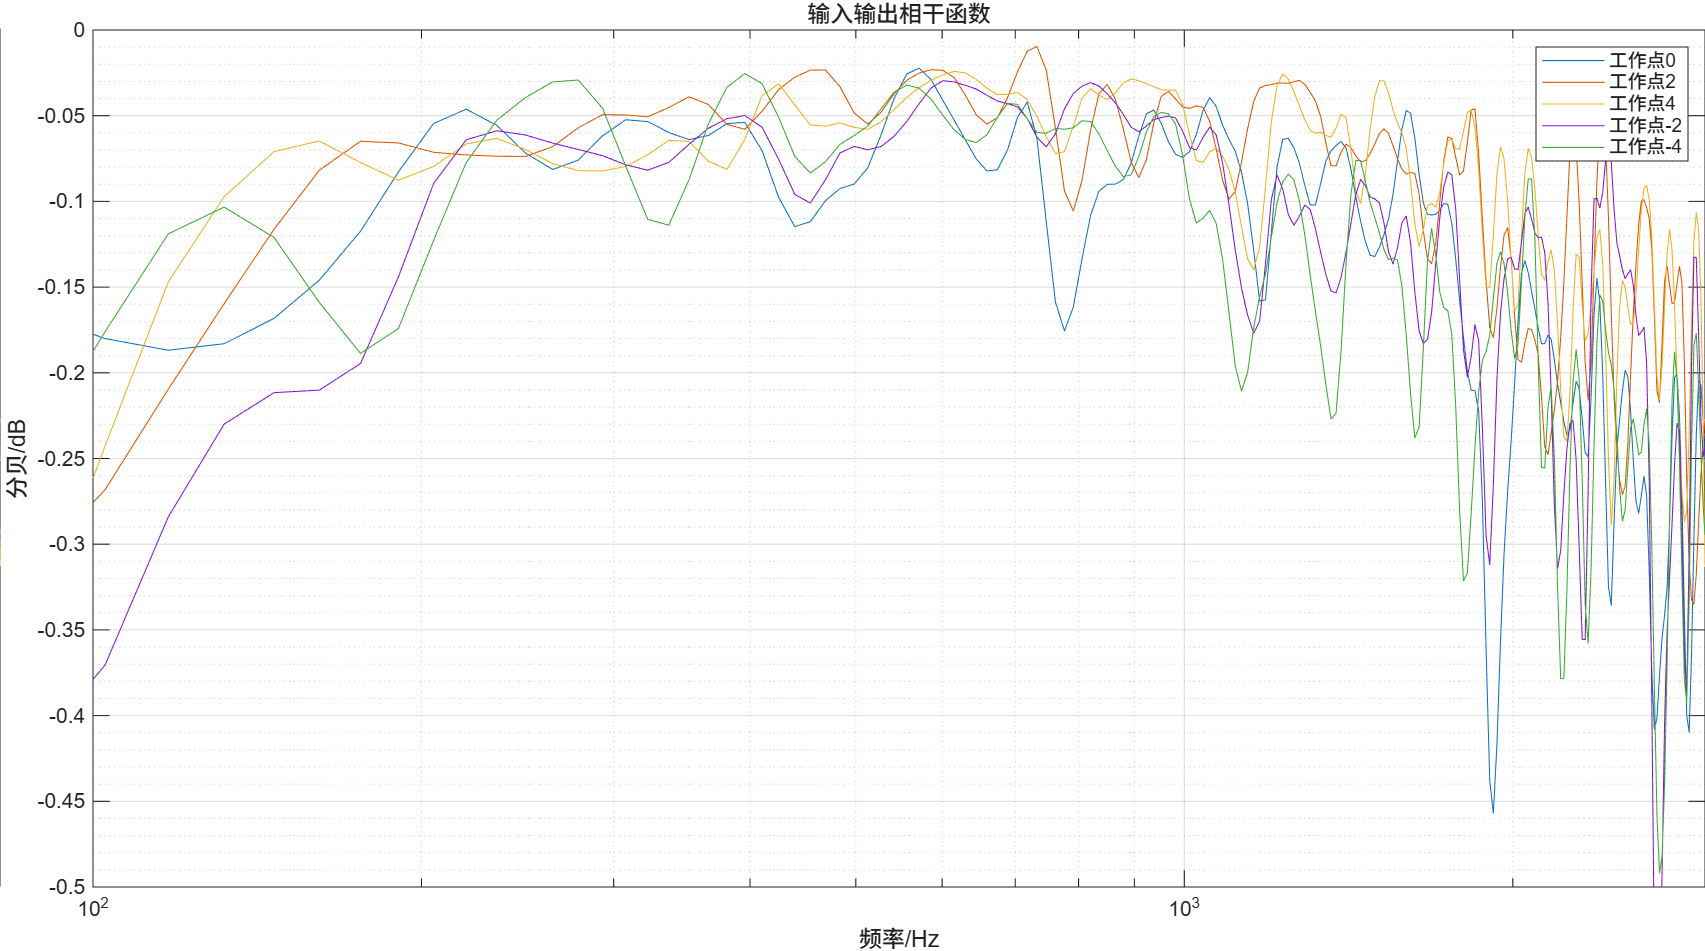
\includegraphics[width=\textwidth]
        {图片/D轴同步电感辨识相干函数.png}
        \caption{D轴同步电感辨识的相干函数}
        \label{fig:D轴同步电感辨识的相干函数}
    \end{minipage}
    \begin{minipage}{0.5\textwidth}
        \centering
        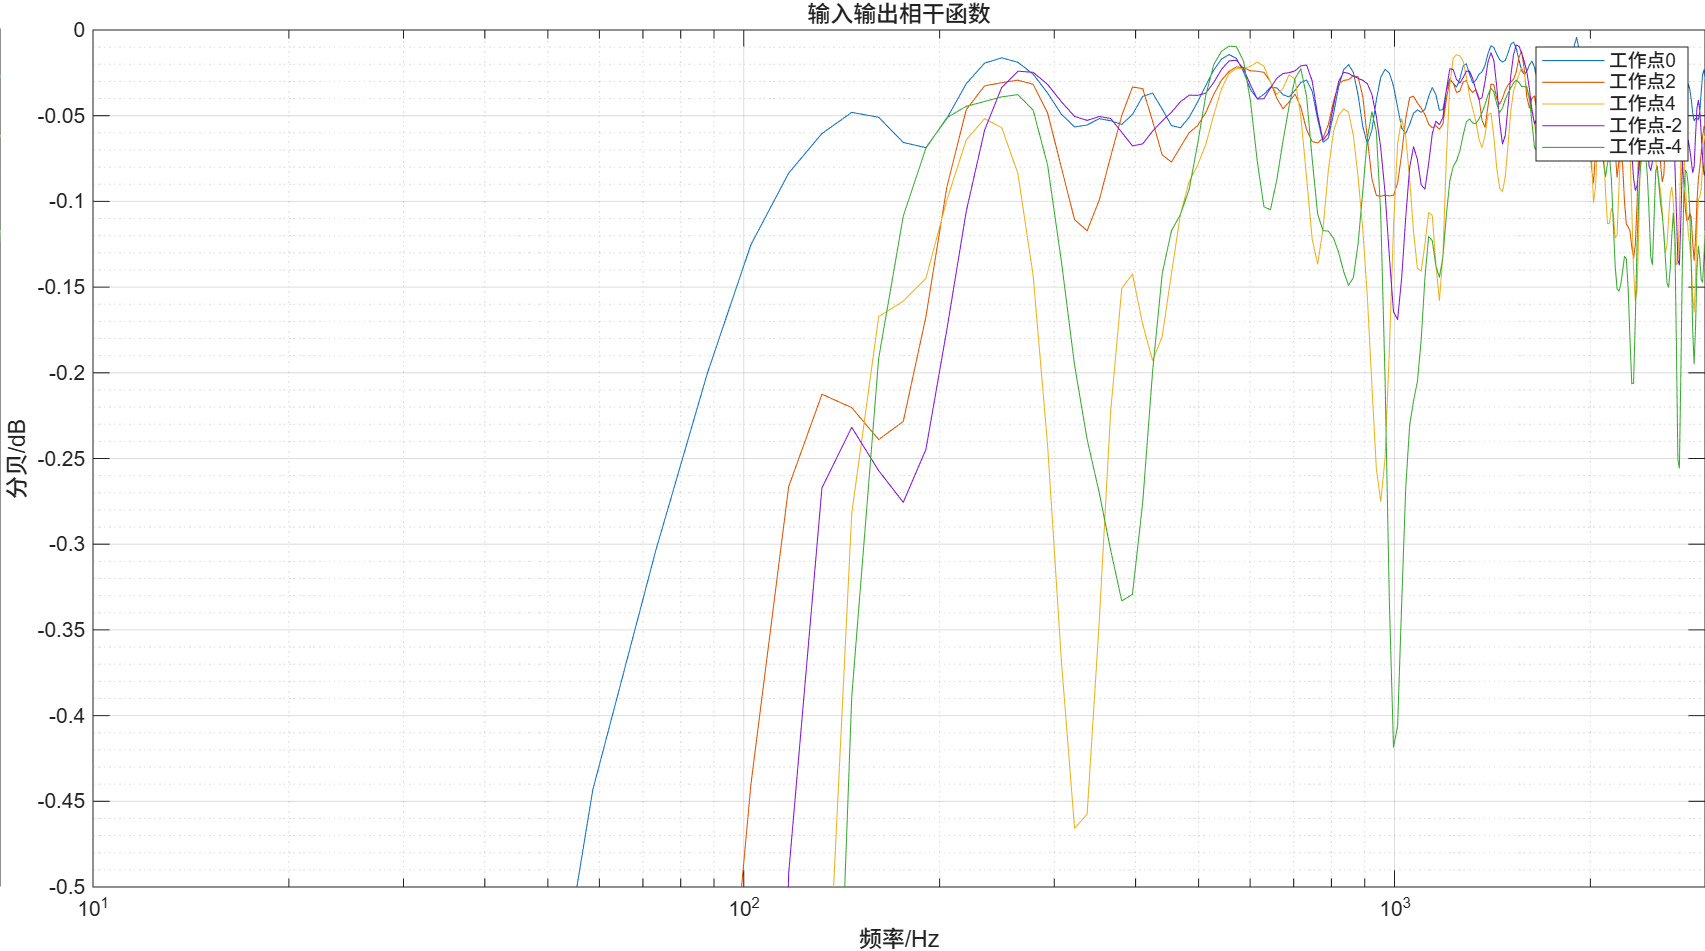
\includegraphics[width=\textwidth]
        {图片/Q轴同步电感辨识相干函数.png}
        \caption{Q轴同步电感辨识的相干函数}
        \label{fig:Q轴同步电感辨识的相干函数}
    \end{minipage}
\end{figure}

可以发现，D轴辨识时无电磁转矩、系统开环，相干函数在关注频段内均满足
\(\gamma^2_{\text{dB}} > -0.5\,\text{dB}\)，信噪比高，辨识可信度高。
Q轴辨识通过重构等效输入近似为开环（但是闭环的物理结构依然存在），相干函数整体较D轴有所下降，
且在出现相干函数谷值（如1kHz附近）。但在电路模态的核心频段（\(400\text{Hz}\sim
800\text{Hz}\)，即RL转折频率附近），Q轴相干函数仍能维持在\(-0.5\,\text{dB}\)
以上，说明即使理论有偏，工程上该偏差可以近似忽略。

接下来分析直接法与间接法在反电动势闭环结构下的表现，工作点取
\(U_{\mathrm{q}} = \pm 2\,\text{V}, \pm 4\,\text{V}\)
\footnote{相较于电路模态辨识少了0V工作点。0V附近静摩擦、转矩死区等
非线性因素主导，辨识结果与其他工作点截然不同，因此不纳入考虑。}
仍将\(\gamma^2_{\text{dB}} > -0.5\,\text{dB}\)视为工程可靠区间。机械动态远慢于电气动态，
其转折频率通常在数赫兹至数十赫兹量级，选取\(1\,\text{Hz}\sim 300\,\text{Hz}\)覆盖机械动态的主要信息区间。相干函数如下所示。
\begin{figure}[H]
    \begin{minipage}{0.5\textwidth}
        \centering
        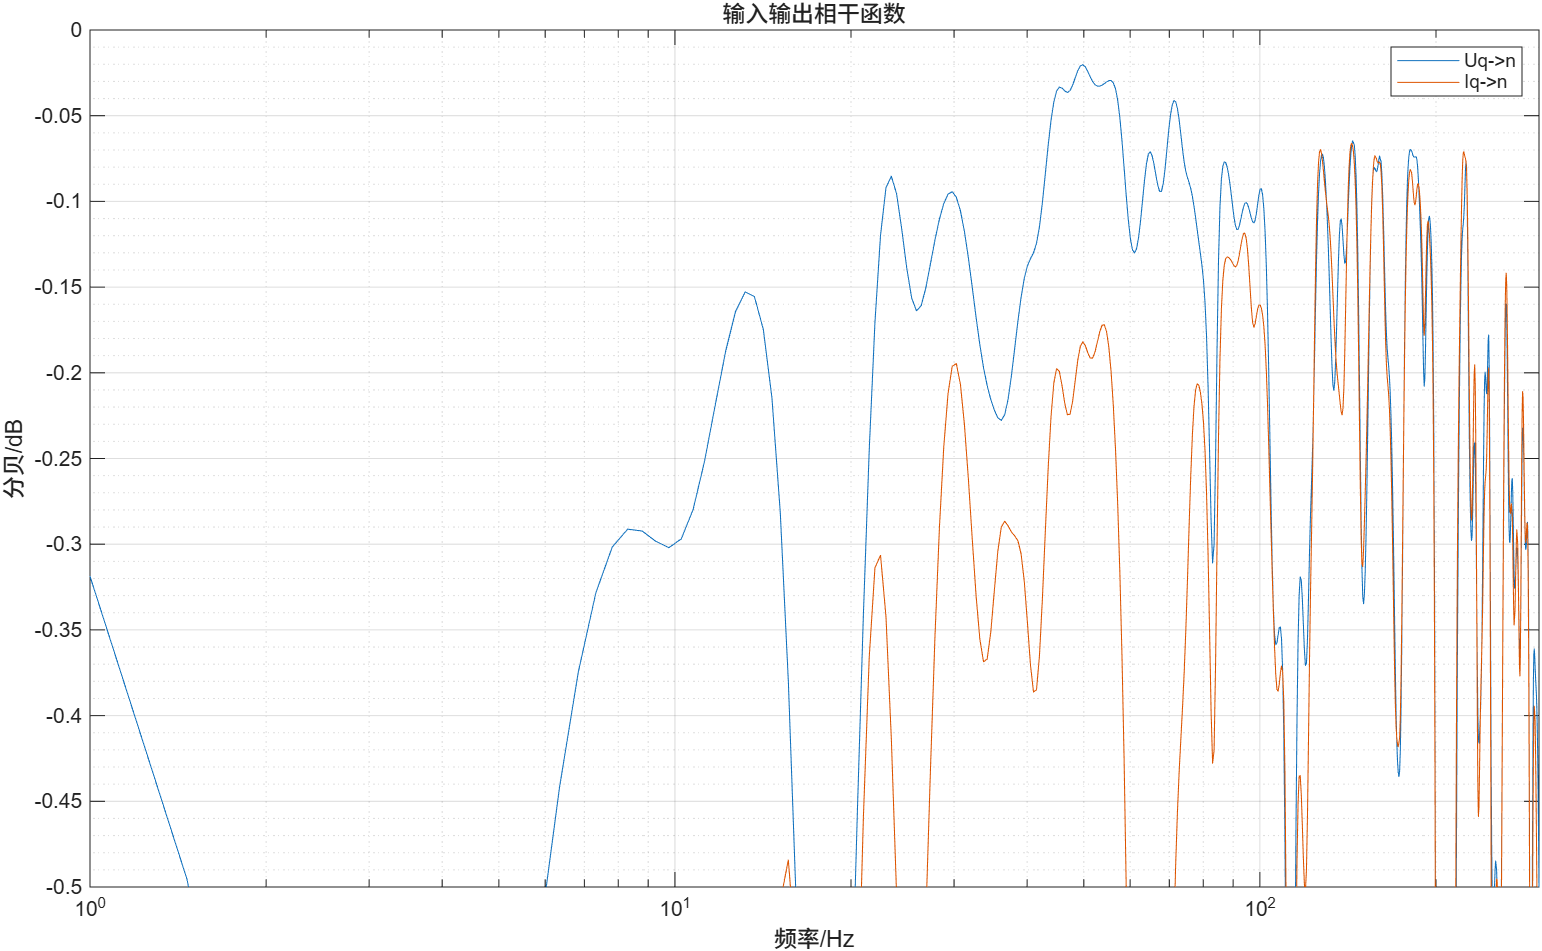
\includegraphics[width=\textwidth]
        {图片/速度环相干函数（-4V）.png}
        \caption{速度环相干函数（-4V）}
        \label{fig:速度环相干函数（-4V）}
    \end{minipage}
    \begin{minipage}{0.5\textwidth}
        \centering
        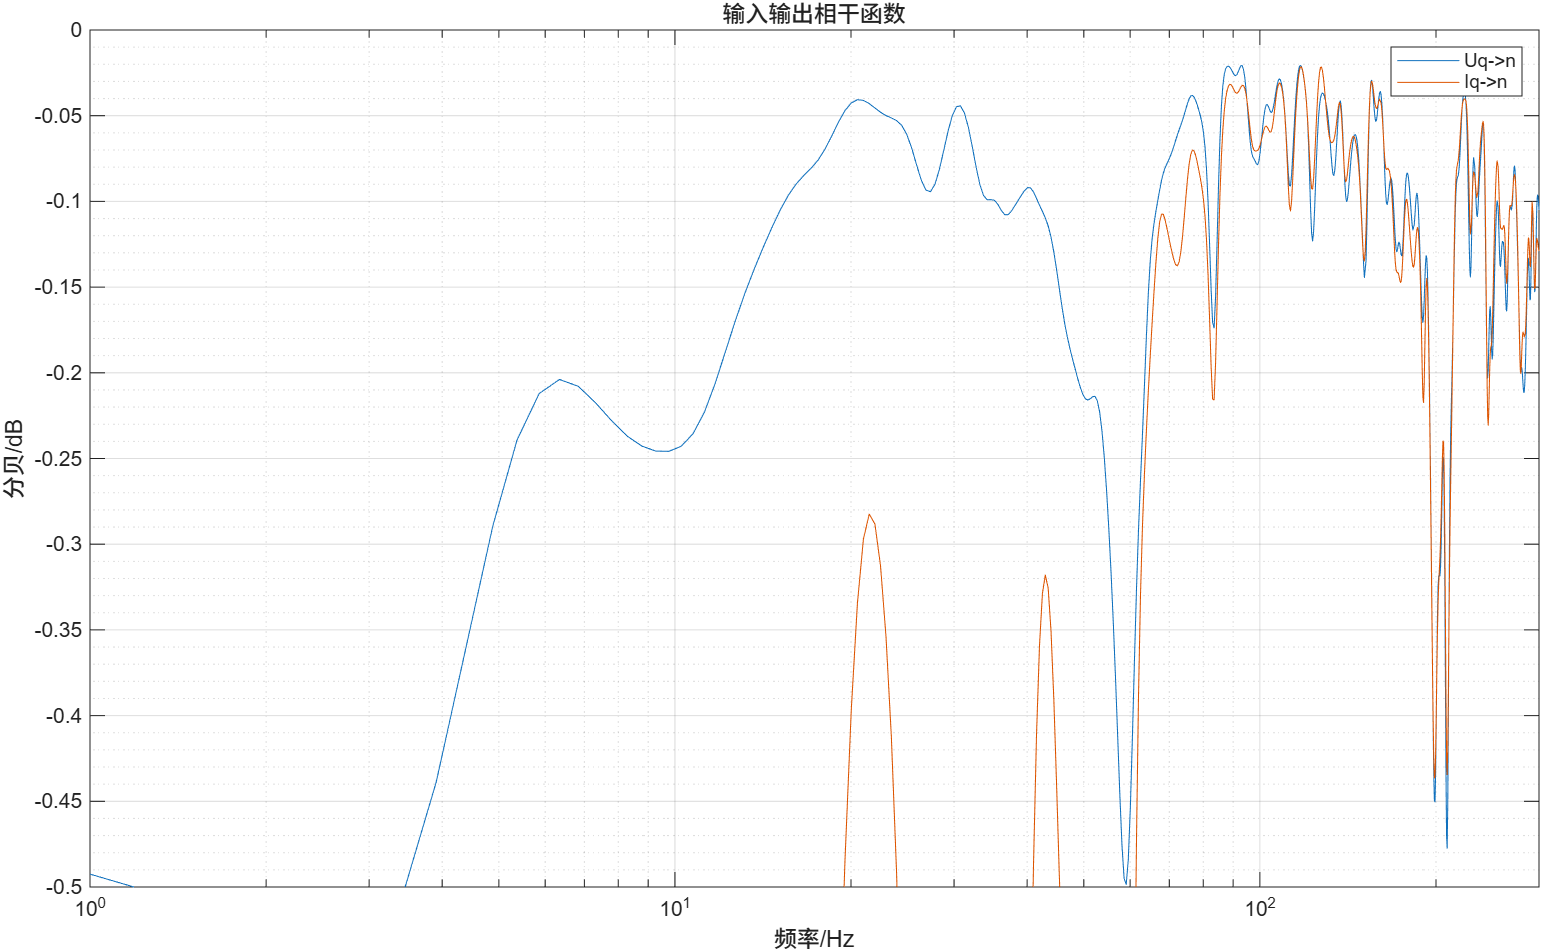
\includegraphics[width=\textwidth]
        {图片/速度环相干函数（-2V）.png}
        \caption{速度环相干函数（-2V）}
        \label{fig:速度环相干函数（-2V）}
    \end{minipage}
\end{figure}
\begin{figure}[H]
    \begin{minipage}{0.5\textwidth}
        \centering
        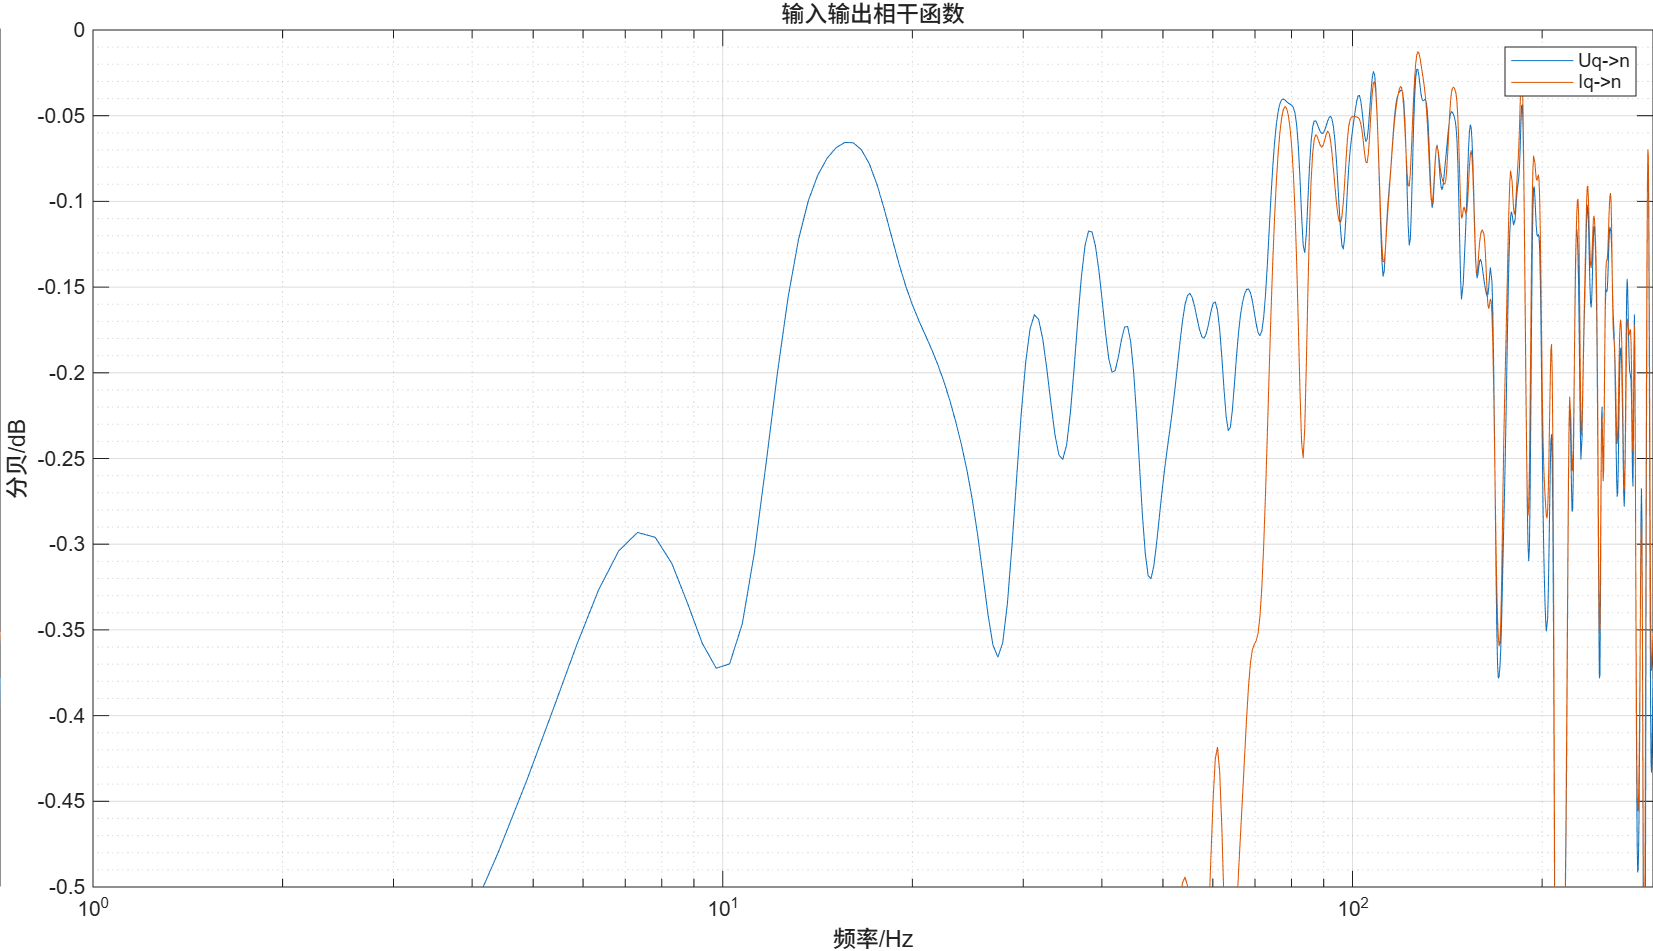
\includegraphics[width=\textwidth]
        {图片/速度环相干函数（2V）.png}
        \caption{速度环相干函数（2V）}
        \label{fig:速度环相干函数（2V）}
    \end{minipage}
    \begin{minipage}{0.5\textwidth}
        \centering
        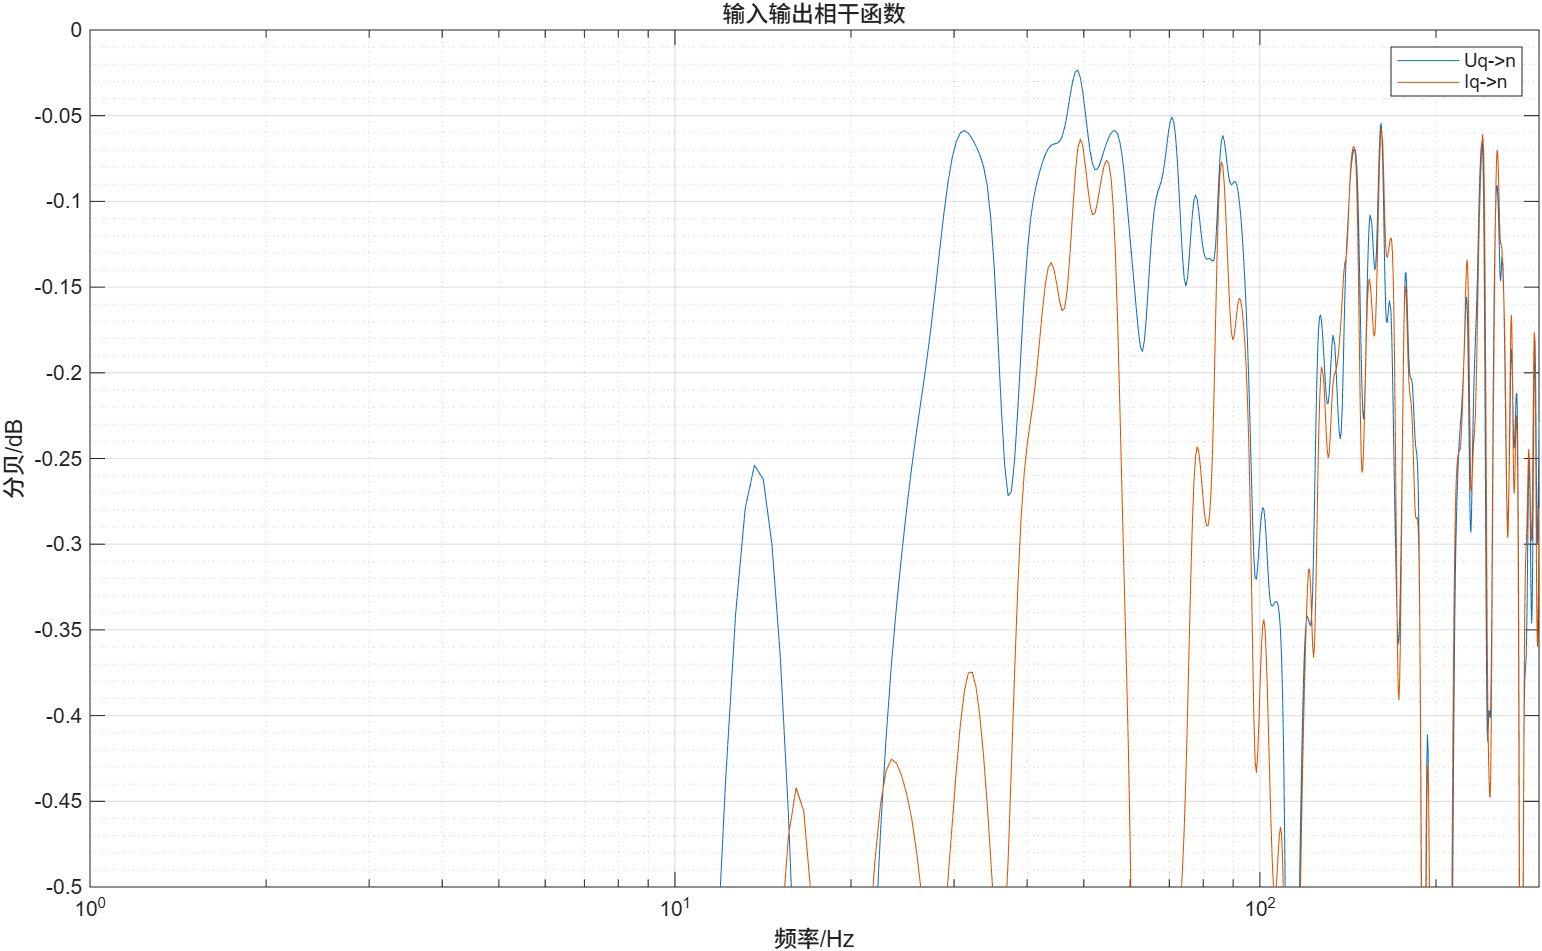
\includegraphics[width=\textwidth]
        {图片/速度环相干函数（4V）.png}
        \caption{速度环相干函数（4V）}
        \label{fig:速度环相干函数（4V）}
    \end{minipage}
\end{figure}

可以发现，直接法的相干函数在核心频段（\(10\,\text{Hz}\sim 100\,\text{Hz}\)）内
普遍较低，估计质量不可靠；间接法的相干函数虽整体优于直接法，
但仍明显低于电路模态的辨识结果。两者在机械动态中相干函数整体偏低，根本原因
在于机械部分的非线性因素（静摩擦、转矩死区、机械系统阶次不定等）无论从数量
还是强度均远超电路部分。
\footnote{另一种理解两者差异的角度是奇异摄动。电机的电路部分和机械部分时间常数尺度差异大，
（电路时间常数\(\cfrac{L_{\mathrm{q}}}{R_{\mathrm{s}}}\approx 0.3\text{ms}\)，而根据后续机械部分传递函数的主导极点
可知主导时间常数约\(\cfrac{1}{30}\text{s}=33.33\text{ms}\)，分离比\(\cfrac{0.3}{33.33}\approx 0.009\ll 1\)）
构成天然奇异摄动系统。辨识快模态（电路部分）时，慢模态（转速）在电气激励时间尺度上近似不变，
反电动势近似为常数，反馈回路基本没有激活。辨识慢模态（机械部分）时，
转速随激励同步变化，反电动势反馈回路在机械时间尺度上被完全激活，辨识结果可靠性显著降低。}
而直接法在闭环情况下还存在数学可证明的严格有偏，因此相干函数值更低。

综上，对机械传递函数的辨识应优先采用间接法：先辨识
\(U_{\mathrm{q}}\to n\)的闭环传递函数，再从已确定的Q轴电路传递函数中代数反推
\(G_{\mathrm{m}}(s)\)。间接法的优势是根本性的，如\ref{sec:输入直接到输出}所述，当以给定无噪信号
\(U_{\mathrm{q}}\)作为输入时，输入与输出测量噪声不相关，维纳-霍普夫方程能够无偏估计该通道的脉冲响应。

\subsection{速度环被控对象辨识与开环验证}
\subsubsection{\(i_{\mathrm{d}}=0\)理想化假设分析}
前文建立了基于\(i_{\mathrm{d}}^*=0\)假设的间接法辨识框架：将\(U_{\mathrm{q}}\)到\(n\)的通道建模为
反电动势闭环结构，其核心在于认为\(i_{\mathrm{d}}\approx 0\)在辨识过程中始终成立，从而使反电动势
\(E=\omega_{\mathrm{e}}(\psi_{\mathrm{m}}+L_{\mathrm{d}}i_{\mathrm{d}})\)简化为\(\omega_{\mathrm{e}}\psi_{\mathrm{m}}\)、电磁转矩
\(T_{\mathrm{e}}=\cfrac{3}{2}p[\psi_{\mathrm{m}}i_{\mathrm{q}}+(L_{\mathrm{d}}-L_{\mathrm{q}})i_{\mathrm{d}}i_{\mathrm{q}}]\)简化为\(\cfrac{3}{2}p\psi_{\mathrm{m}}i_{\mathrm{q}}\)。
然而实际辨识过程中，\(i_{\mathrm{d}}^*=0\)仅代表控制器的给定目标，由于D轴电流环有限带宽、采样噪声及
交叉耦合\(\omega_{\mathrm{e}}L_{\mathrm{q}}i_{\mathrm{q}}\)的扰动，实测\(i_{\mathrm{d}}\)不可避免存在微小偏差。若该偏差导致反电动势
或电磁转矩的简化值与实际值差异显著，则间接法的建模基础将不再成立。因此，有必要在用辨识
结果反推\(G_{\mathrm{m}}(s)\)之前，先验证\(i_{\mathrm{d}}=0\)假设在实验数据中的工程成立性。

以\(U_{\mathrm{q}}=2\text{V}\)为代表性工作点，在M序列激励的全时段内，利用实测的\(i_{\mathrm{d}}(t)\)，
\(i_{\mathrm{q}}(t)\)和\(n(t)\)数据，分别计算反电动势与电磁转矩在两种情形下的取值并进行对比：
\begin{itemize}
    \item \(i_{\mathrm{d}}=0\)理想假设：计算\(E_{\mathrm{0}}=\omega_{\mathrm{e}}\psi_{\mathrm{m}}=\cfrac{\pi}{30}n(t)p\psi_{\mathrm{m}}\)和
    \(T_{\mathrm{e0}}=\cfrac{3}{2}p\psi_{\mathrm{m}}i_{\mathrm{q}}(t)\)。
    \item 实测\(i_{\mathrm{d}}\)代入：计算\(E_{\text{meas}}=\cfrac{\pi}{30}n(t)p[\psi_{\mathrm{m}}+L_{\mathrm{d}}i_{\mathrm{d}}(t)]\)和
    \(T_{e,\text{meas}}=\cfrac{3}{2}p[\psi_{\mathrm{m}}i_{\mathrm{q}}(t)+(L_{\mathrm{d}}-L_{\mathrm{q}})i_{\mathrm{d}}(t)i_{\mathrm{q}}(t)]\)，其中
    \(p=14\)，\(\psi_{\mathrm{m}}\)，\(L_{\mathrm{d}}\)，\(L_{\mathrm{q}}\)取自第四章辨识结果。
\end{itemize}
对比结果如下图所示。
\begin{figure}[H]
    \begin{minipage}{0.5\textwidth}
        \centering
        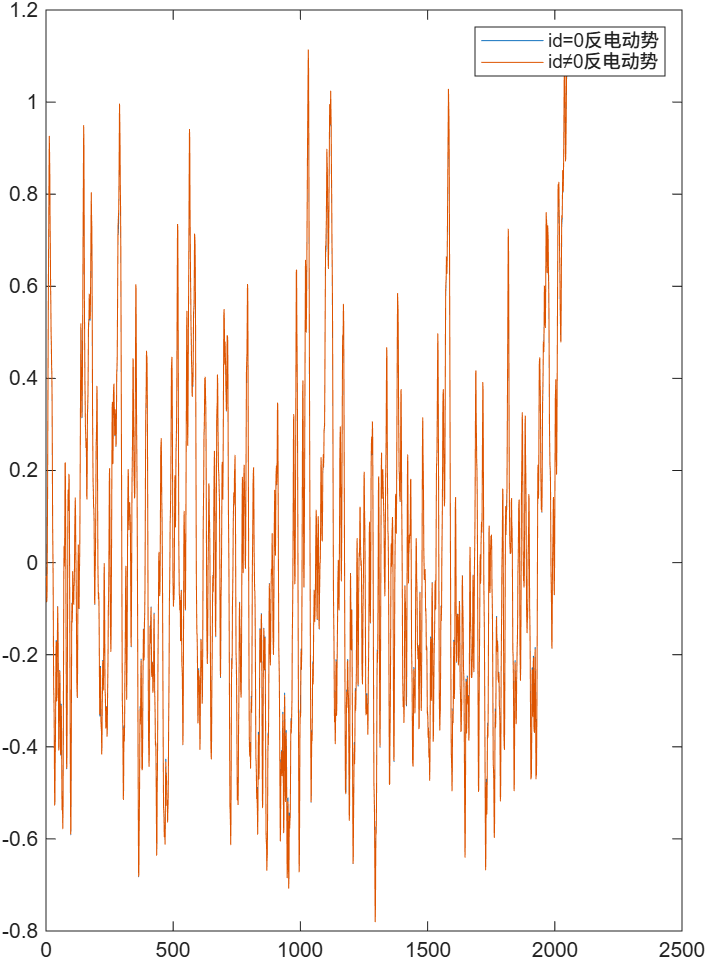
\includegraphics[width=\textwidth]
        {图片/速度环工作点2V反电动势对比.png}
        \caption{速度环工作点2V反电动势对比}
    \end{minipage}
    \begin{minipage}{0.5\textwidth}
        \centering
        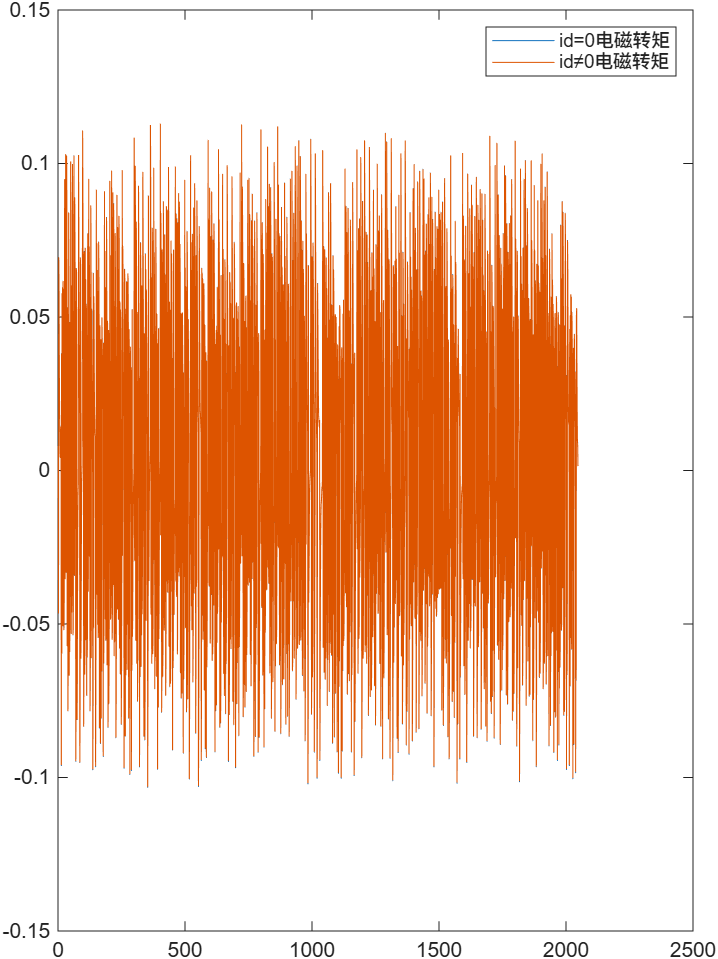
\includegraphics[width=\textwidth]
        {图片/速度环工作点2V电磁转矩对比.png}
        \caption{速度环工作点2V电磁转矩对比}
    \end{minipage}
    \label{fig:速度环工作点2V理想id与实际id对比}
\end{figure}

据上图可知，两者在反电动势和电磁转矩两条曲线上的差异均微乎其微，波形在时域上几乎完全重合。
为覆盖不同工作点下的情况，在\(U_{\mathrm{q}}=\pm2\text{V},\pm4\text{V}\)四个工作点均进行上述分析，
计算反电动势和电磁转矩在理想\(i_{\mathrm{d}}=0\)与实际\(i_{\mathrm{d}}\)下的相关系数与拟合优度，汇总如下表所示。
\begin{table}[H]
    \centering
    \begin{tabular}{|c|c|c|c|c|}
        \hline
        \multirow{2}{*}{工作点} & \multicolumn{2}{c|}{反电动势} & \multicolumn{2}{c|}{电磁转矩}\\
        \cline{2-5}
        & 相关系数 & 拟合优度 & 相关系数 & 拟合优度\\
        \hline
        \(U_{\mathrm{q}}=2\text{V}\) & 99.99991\% & 99.86604\% & 100.00000\% & 99.97521\%\\
        \hline
        \(U_{\mathrm{q}}=4\text{V}\) & 99.99987\% & 99.83449\% & 100.00000\% & 99.96860\%\\
        \hline
        \(U_{\mathrm{q}}=-2\text{V}\) & 99.99992\% & 99.86799\% & 100.00000\% & 99.97689\%\\
        \hline
        \(U_{\mathrm{q}}=-4\text{V}\) & 99.99985\% & 99.81871\% & 100.00000\% & 99.96570\%\\
        \hline
    \end{tabular}
    \caption{各工作点下\(i_{\mathrm{d}}=0\)理想假设与实测\(i_{\mathrm{d}}\)的差异评估}
    \label{tab:各工作点id=0假设验证汇总}
\end{table}

由表\ref{tab:各工作点id=0假设验证汇总}可知，四个工作点下的反电动势与电磁转矩的相关系数和
拟合优度均超过99.5\%，\(i_{\mathrm{d}}=0\)的简化假设在所有工作点下均完全成立。据此，可以确信后续基于
\(i_{\mathrm{d}}=0\)理想模型进行的间接法辨识及机械传递函数反推具备充分的工程合理性。

\subsubsection{不同工作点的机械部分传递函数辨识}
满足了\(i_{\mathrm{d}}=0\)的理想化近似条件后，才能真正开始基于间接法的机械传递函数辨识。
在\(U_{\mathrm{q}}=2V\)工作点附近给予伪随机激励，幅值2V，辨识从\(U_{\mathrm{q}}\)到\(n\)的传递函数，奇异值分解如下图所示和
数值解-解析解频域对比如下图所示。幅频相关系数99.08708\%，相频相关系数99.91204\%，复频率
拟合优度88.14769\%。根据奇异值分解图可得闭环传递函数应为2阶。辨识得到离散传递函数为：
\footnote{由于伪随机信号对直流增益几乎没有辨识能力，因此选取阶跃段的稳态值，除以激励值作为直流增益，
修正辨识结果。}
\(G(z)=\cfrac{195+1111z^{-1}}{60.17-51.9z^{-1}+12.32z^{-2}}\)。
\begin{figure}[H]
    \begin{minipage}{0.5\textwidth}
        \centering
        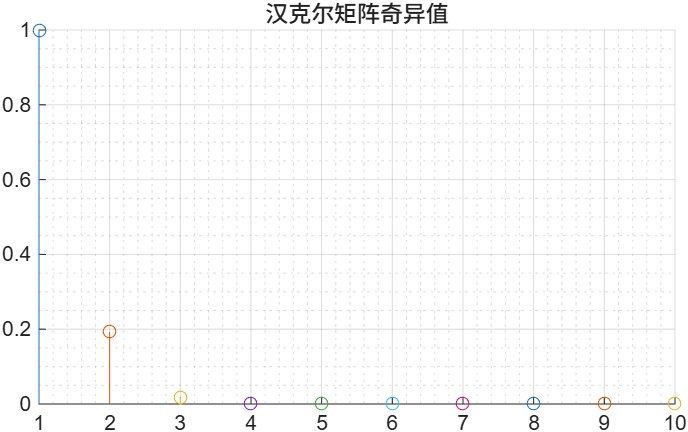
\includegraphics[width=\textwidth]
        {图片/速度环工作点2V奇异值分解图.jpg}
        \caption{速度环工作点2V奇异值分解图}
    \end{minipage}
    \begin{minipage}{0.5\textwidth}
        \centering
        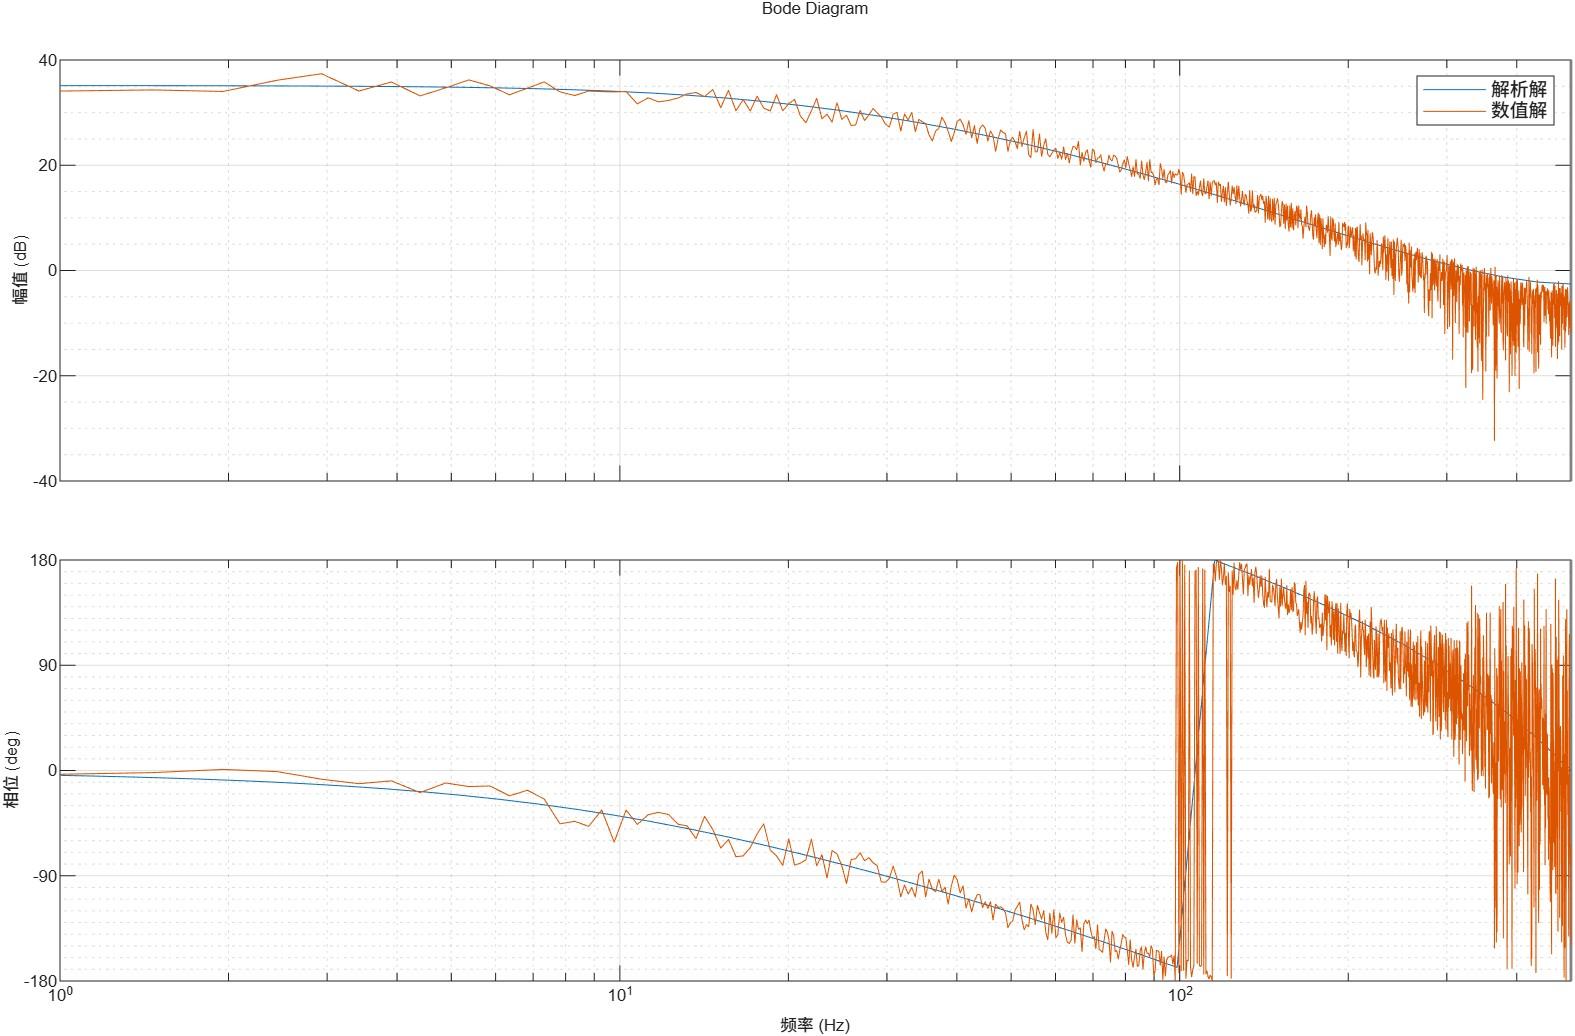
\includegraphics[width=\textwidth]
        {图片/速度环工作点2V数值解和解析解对比.jpg}
        \caption{速度环工作点2V数值解和解析解对比}
    \end{minipage}
\end{figure}

使用MATLAB的d2c命令，在零阶保持器ZOH作用下将辨识得到的闭环传递函数映射到连续域中，可得连续闭环传递函数
\(G(s)=\cfrac{-2.34\times 10^{4}s+4.578\times 10^7}{s^2+1586s+7.234\times 10^5}\)。根据图\ref{fig:Q轴电流-速度系统框图}
可知，闭环传递函数和机械部分的传递函数满足：
\begin{equation}
    G(s)=\cfrac{\cfrac{1}{R_{\mathrm{s}}+L_{\mathrm{q}}s}\times\cfrac{3}{2}p\psi_{\mathrm{m}}\times G_{\mathrm{m}}(s)}
    {1+\cfrac{1}{R_{\mathrm{s}}+L_{\mathrm{q}}s}\times\cfrac{3}{2}p\psi_{\mathrm{m}}\times G_{\mathrm{m}}(s)\times \cfrac{\pi}{30}p\psi_{\mathrm{m}}}
    \label{eq:Q轴电流-速度闭环传递函数表达式}
\end{equation}

推导可得：
\begin{equation}
    G_{\mathrm{m}}(s)=\cfrac{(R+L_{\mathrm{q}}s)G(s)}{\cfrac{3}{2}p\psi_{\mathrm{m}}[1-\cfrac{\pi}{30}p\psi_{\mathrm{m}}G(s)]}
    \label{eq:机械部分传递函数表达式}
\end{equation}

因此可得在2V工作点附近辨识得到的机械部分传递函数为
\begin{equation*}
    G_{\mathrm{m}}(s)=\cfrac{-50.76 s^4 - 1.145\times 10^5 s^3 + 1.709\times 10^8 s^2 + 
    3.901\times 10^{11} s + 1.892\times 10^{14}}
    {0.2028 s^4 + 710.2 s^3 + 7.781\times 10^{5} s^2 + 3.05\times 10^{8} s + 1.087\times 10^{10}}
\end{equation*}

机械部分传递函数看似为四阶，实际上为二阶，这是因为传递函数代数运算精度不足没能完全对消。求解上述传递函数的零极点结果为：
零点：[-2629.4、1959.4、-792.8±j307.9]；极点：[-1877.6、-792.8±j307.9、-39.5]。其中零点-792.8±j307.9和
极点-792.8±j307.9可以对消
\footnote{MATLAB显示精度问题，使得两个零极点看起来完全一致，实际上略有不同才导致没能完全抵消。但零极点的差异在该
数量级上可以忽略，视为对消}
。因此最终只剩下两个零点[-2629.4、1959.4]和
两个极点[-1877.6,-39.5]。而直流增益为[17398]。

后续其他工作点也按照上述方法进行，先辨识2阶的闭环传递函数，使用d2c命令在zoh选项下连续化得到连续域的闭环传递函数，
通过\eqref{eq:机械部分传递函数表达式}代数计算得到机械部分传递函数，将可以对消的零极点对消后按照两个零点、
两个极点和直流增益表征辨识结果。

工作点4V的闭环传递函数辨识结果如下图所示，幅频相关系数98.41397\%，相频相关系数99.79761\%，复频率
拟合优度83.84955\%。辨识得到离散传递函数为：\(G(z)=\cfrac{198.9+1150z^{-1}}{61.02-52.8z^{-1}+12.06z^{-2}}\)。
\begin{figure}[H]
    \begin{minipage}{0.5\textwidth}
        \centering
        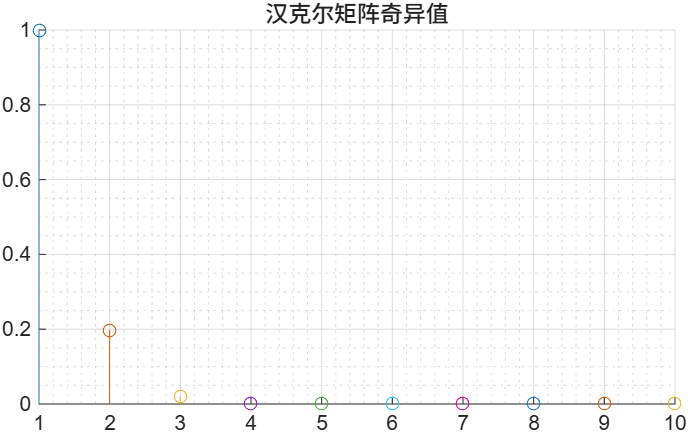
\includegraphics[width=\textwidth]
        {图片/速度环工作点4V奇异值分解图.png}
        \caption{速度环工作点4V奇异值分解图}
    \end{minipage}
    \begin{minipage}{0.5\textwidth}
        \centering
        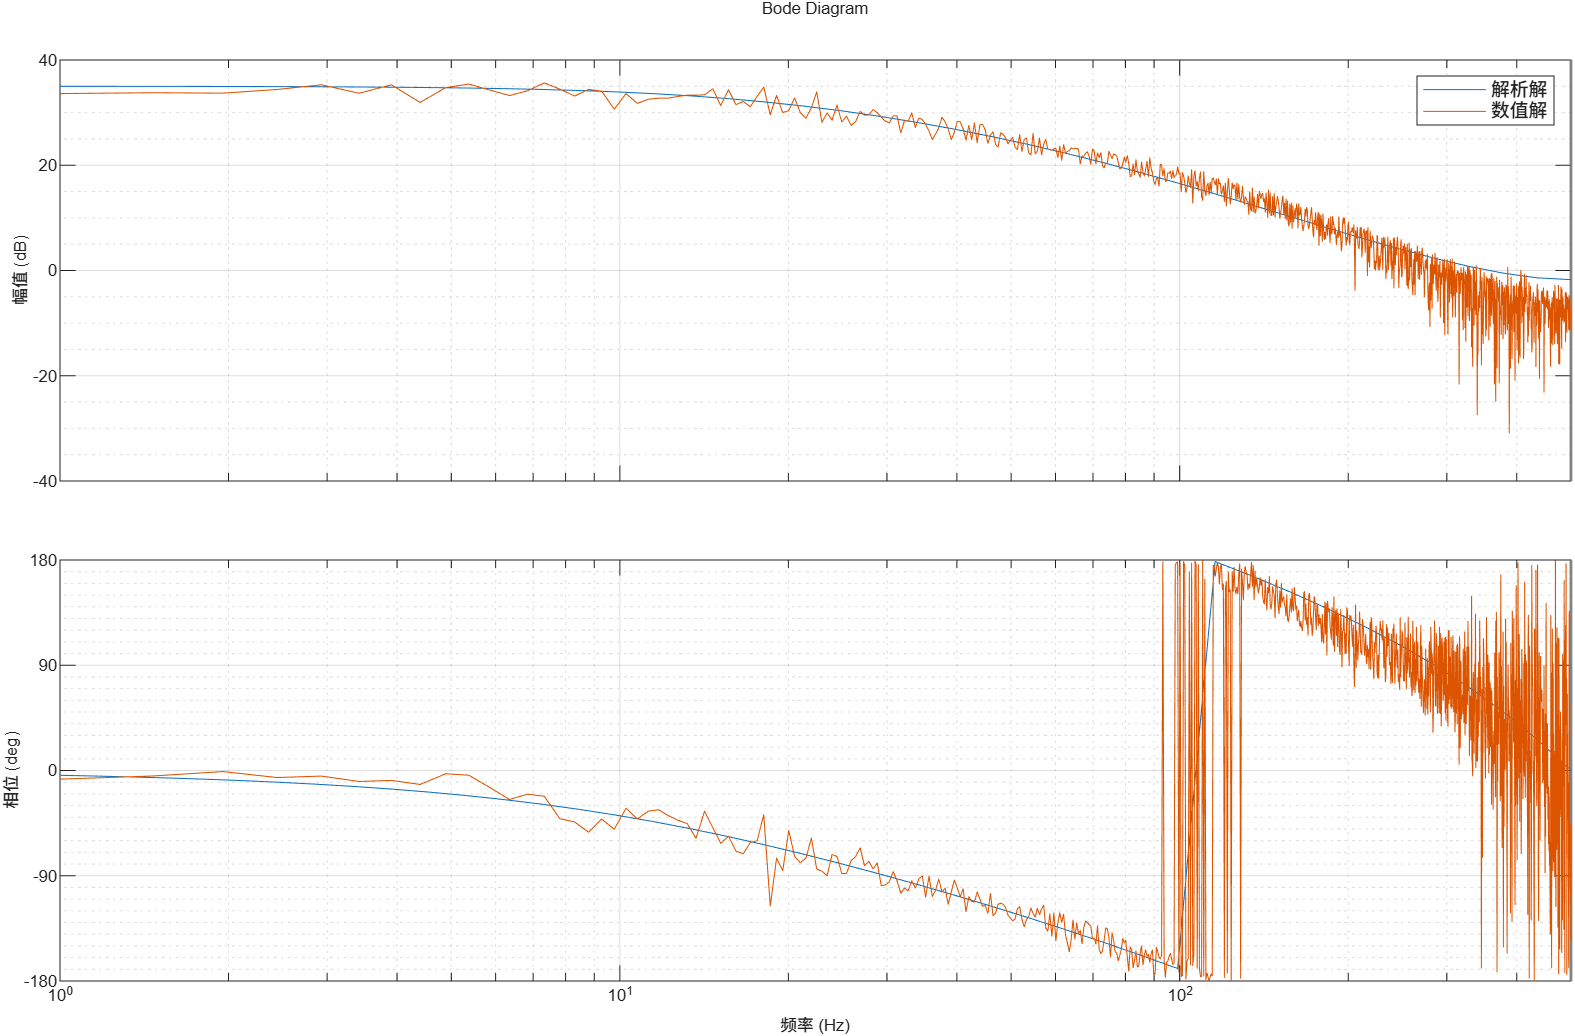
\includegraphics[width=\textwidth]
        {图片/速度环工作点4V数值解和解析解对比.png}
        \caption{速度环工作点4V数值解和解析解对比}
    \end{minipage}
\end{figure}
连续化、反推机械部分传递函数并消去零极点后得到零点[-2629.4,1943.5]和极点[-1945.1,-21]，直流增益[32510]
（零极点-810.7±j231.1对消）。

工作点-2V的闭环传递函数辨识结果如下图所示，幅频相关系数98.97118\%，相频相关系数99.91117\%，复频率
拟合优度87.59657\%。辨识得到离散传递函数为：\(G(z)=\cfrac{198.6+1126z^{-1}}{59.41-51.02z^{-1}+12.35z^{-2}}\)。
\begin{figure}[H]
    \begin{minipage}{0.5\textwidth}
        \centering
        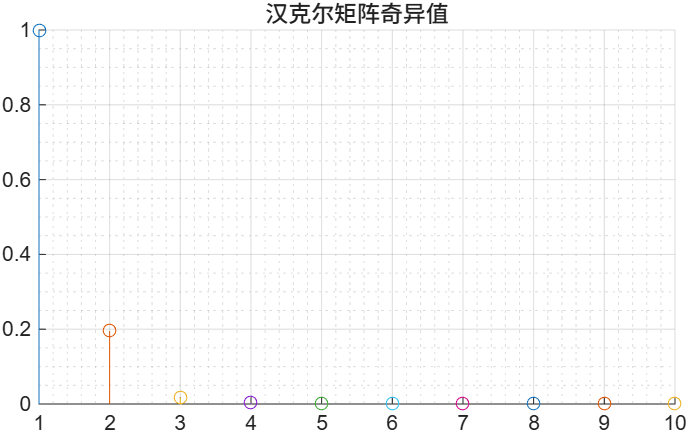
\includegraphics[width=\textwidth]
        {图片/速度环工作点-2V奇异值分解图.png}
        \caption{速度环工作点-2V奇异值分解图}
    \end{minipage}
    \begin{minipage}{0.5\textwidth}
        \centering
        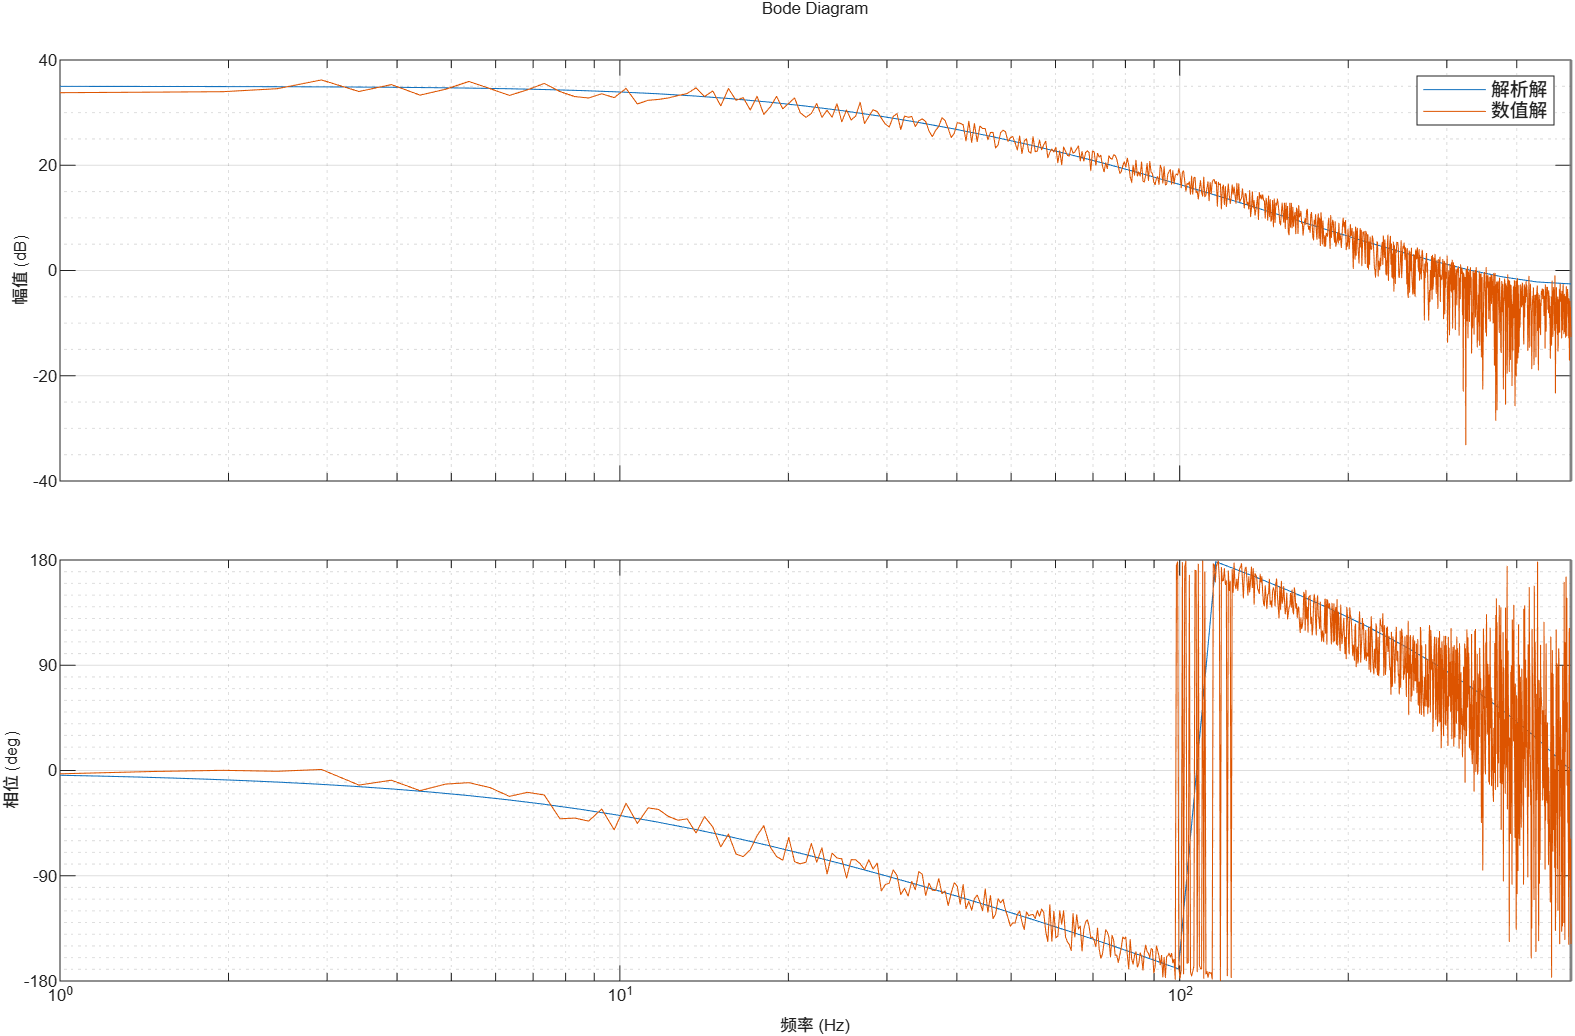
\includegraphics[width=\textwidth]
        {图片/速度环工作点-2V数值解和解析解对比.png}
        \caption{速度环工作点-2V数值解和解析解对比}
    \end{minipage}
\end{figure}
连续化、反推机械部分传递函数并消去零极点后得到零点[-2629.4,1964.2]和极点[-1870.7,-37.9]，直流增益[18622]
（零极点-785.3±j343.5对消）。

工作点-4V的闭环传递函数辨识结果如下图所示，幅频相关系数98.51759\%，相频相关系数99.76702\%，复频率
拟合优度84.81924\%。辨识得到离散传递函数为：\(G(z)=\cfrac{205.5+1146z^{-1}}{60.76-52.04z^{-1}+11.91z^{-2}}\)。
\begin{figure}[H]
    \begin{minipage}{0.5\textwidth}
        \centering
        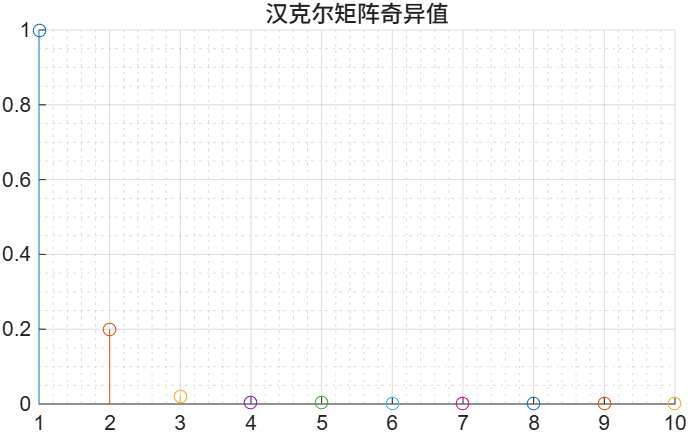
\includegraphics[width=\textwidth]
        {图片/速度环工作点-4V奇异值分解图.png}
        \caption{速度环工作点-4V奇异值分解图}
    \end{minipage}
    \begin{minipage}{0.5\textwidth}
        \centering
        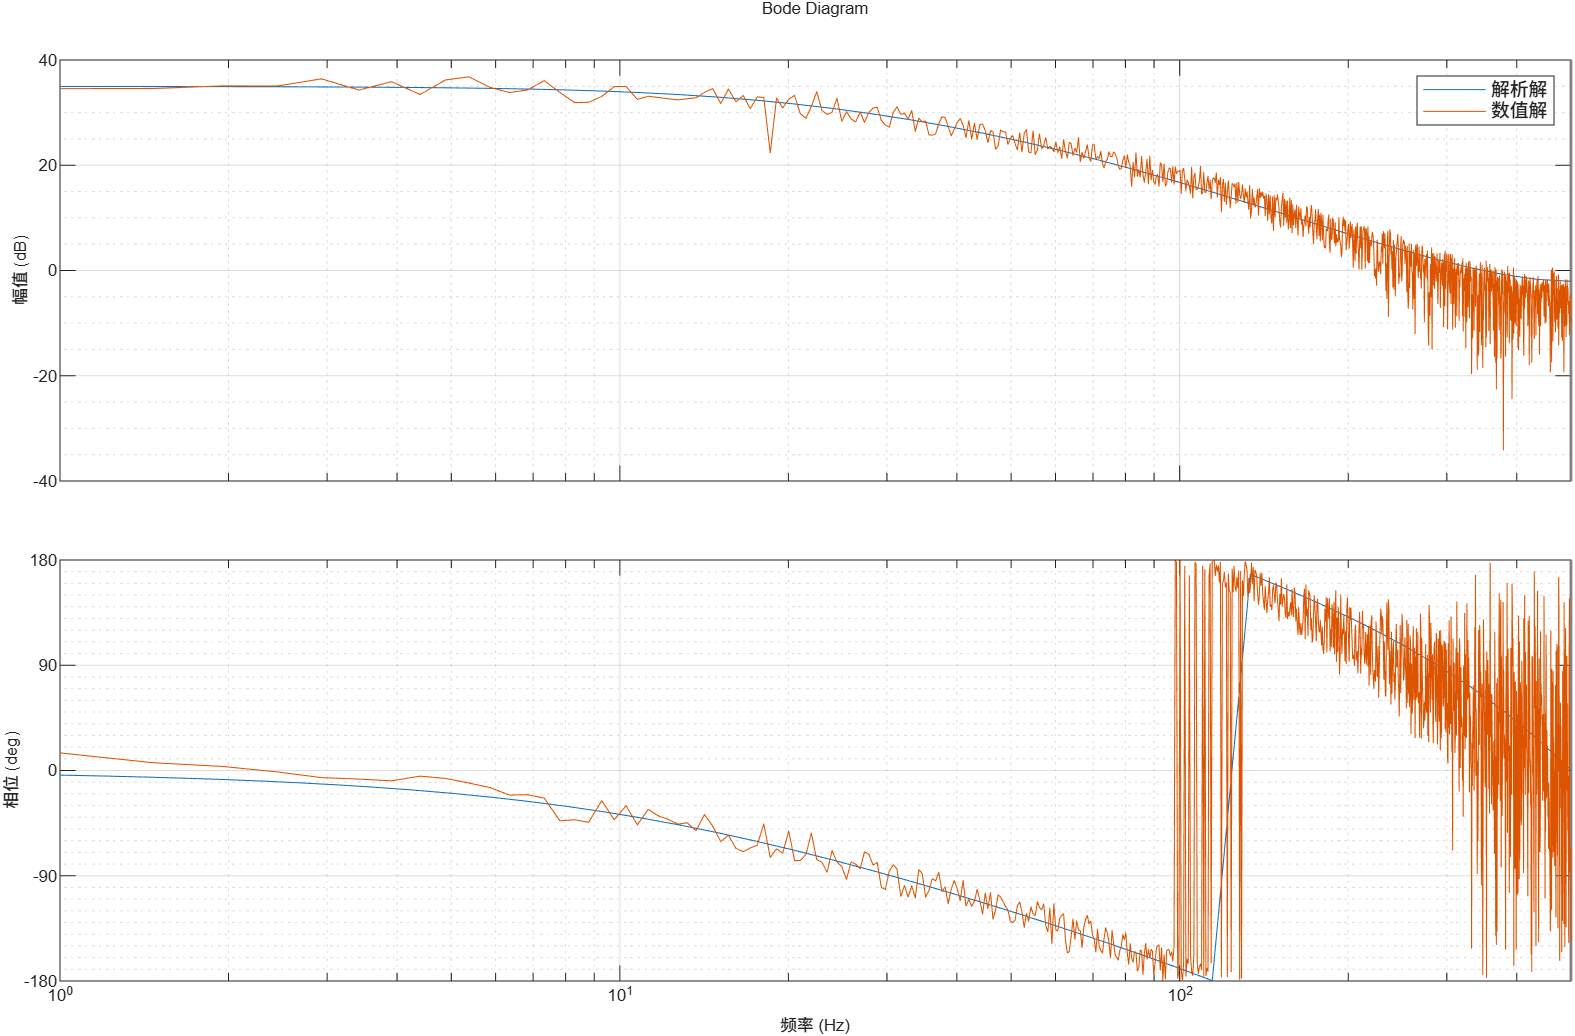
\includegraphics[width=\textwidth]
        {图片/速度环工作点-4V数值解和解析解对比.png}
        \caption{速度环工作点-4V数值解和解析解对比}
    \end{minipage}
\end{figure}
连续化、反推机械部分传递函数并消去零极点后得到零点[-2629.4,1956.0]和极点[-1948.7,-27.1]，直流增益[25478]
（零极点-814.9±j156.0对消）。

将上述四个工作点的机械部分传递函数辨识结果汇总如下表所示。
\begin{table}[H]
    \centering
    \begin{tabular}{|c|c|c|c|c|c|c|}
        \hline
        \multirow{2}{*}{工作点} & \multicolumn{3}{c|}{闭环辨识结果} & \multirow{2}{*}{极点} & \multirow{2}{*}{零点} & \multirow{2}{*}{直流增益} \\
        \cline{2-4}
        & 幅频相关系数 & 相频相关系数 & 拟合优度 & & & \\
        \hline
        \(U_{\mathrm{q}}=-4\text{V}\) & 98.51759\% & 99.76702\% & 84.81924\% & -1948.7, -27.1 & -2629.4, 1956.0 & 25478\\
        \hline
        \(U_{\mathrm{q}}=-2\text{V}\) & 98.97118\% & 99.91117\% & 87.59657\% & -1870.7, -37.9 & -2629.4, 1964.2 & 18622\\
        \hline
        \(U_{\mathrm{q}}=2\text{V}\)  & 99.08708\% & 99.91204\% & 88.14769\% & -1877.6, -39.5 & -2629.4, 1959.4 & 17398\\
        \hline
        \(U_{\mathrm{q}}=4\text{V}\)  & 98.41397\% & 99.79761\% & 83.84955\% & -1945.1, -21.0  & -2629.4, 1943.5 & 32510\\
        \hline
    \end{tabular}
    \caption{各工作点机械部分传递函数\(G_{\mathrm{m}}(s)\)辨识结果汇总}
    \label{tab:各工作点Gm辨识结果汇总}
\end{table}

\subsubsection{反推结果的敏感性分析与辨识模型求解\label{sec:反推结果的敏感性分析}}
实际工程上使用上述方法时，依赖于已经完成辨识的参数的精确度，若已完成辨识的参数误差较大，会导致辨识的机械传递函数
\(G_{\mathrm{m}}(s)\)偏差严重，接下来对此进行简单分析，并说明如何从表\ref{tab:各工作点Gm辨识结果汇总}中
得到较为合适的辨识模型。

反推式\eqref{eq:机械部分传递函数表达式}可改写为乘除结构：
\begin{equation*}
    G_{\mathrm{m}}(s)=\cfrac{R_{\mathrm{s}}+L_{\mathrm{q}}s}{\cfrac{3}{2}p\psi_{\mathrm{m}}}\times G(s)\times\cfrac{1}{1-\cfrac{\pi}{30}p\psi_{\mathrm{m}}G(s)}
\end{equation*}

其中\(R_{\mathrm{s}}\)、\(L_{\mathrm{q}}\)、\(\psi_{\mathrm{m}}\)与辨识得到的\(G(s)\)均存在误差
\footnote{相电阻\(R_{\mathrm{s}}\)、Q轴同步电感\(L_{\mathrm{q}}\)和永磁体磁链\(\psi_{\mathrm{m}}\)为常数，其误差是绝对误差；
闭环传递函数\(G(s)\)的误差指不同频点下复数误差的大小（含幅值与相位）。}。
对上式取对数可得：
\begin{equation*}
    \ln G_{\mathrm{m}}(s)=\ln(R_{\mathrm{s}}+L_{\mathrm{q}}s)+\ln G(s)-\ln\cfrac{3}{2}p\psi_{\mathrm{m}}-\ln[1-\cfrac{\pi}{30}p\psi_{\mathrm{m}}G(s)]
\end{equation*}

那么相对误差的传播公式就是一节全微分的形式：
\begin{align*}
    \cfrac{\Delta G_{\mathrm{m}}(s)}{G_{\mathrm{m}}(s)}&=
    \cfrac{\Delta[R_{\mathrm{s}}+L_{\mathrm{q}}s]}{R_{\mathrm{s}}+L_{\mathrm{q}}s}
    +\cfrac{\Delta G(s)}{G(s)}-\cfrac{\Delta(\cfrac{3}{2}p\psi_{\mathrm{m}})}{\cfrac{3}{2}p\psi_{\mathrm{m}}}
    +\cfrac{\Delta[1-\cfrac{\pi}{30}p\psi_{\mathrm{m}}G(s)]}{1-\cfrac{\pi}{30}p\psi_{\mathrm{m}}G(s)}\\
    &=\cfrac{\Delta R_{\mathrm{s}}+s\Delta L_{\mathrm{q}}}{R_{\mathrm{s}}+L_{\mathrm{q}}s}+
    \cfrac{\Delta G(s)}{G(s)}-\cfrac{\Delta \psi_{\mathrm{m}}}{\psi_{\mathrm{m}}}-
    (-\cfrac{\cfrac{\pi}{30}pG(s)\Delta\psi_{\mathrm{m}}}{1-\cfrac{\pi}{30}p\psi_{\mathrm{m}}G(s)}
    -\cfrac{\cfrac{\pi}{30}p\psi_{\mathrm{m}}\Delta G(s)}{1-\cfrac{\pi}{30}p\psi_{\mathrm{m}}G(s)})\\
    &=\cfrac{R_{\mathrm{s}}}{R_{\mathrm{s}}+s L_{\mathrm{q}}}\cfrac{\Delta R_{\mathrm{s}}}{R_{\mathrm{s}}}+
    \cfrac{s L_{\mathrm{q}}}{R_{\mathrm{s}}+s L_{\mathrm{q}}}\cfrac{\Delta L_{\mathrm{q}}}{L_{\mathrm{q}}}+
    \cfrac{1}{1-\cfrac{\pi}{30}p\psi_{\mathrm{m}}G(s)}\cfrac{\Delta G(s)}{G(s)}+
    \cfrac{\cfrac{\pi}{15}p\psi_{\mathrm{m}}G(s)-1}{1-\cfrac{\pi}{30}p\psi_{\mathrm{m}}G(s)}\cfrac{\Delta\psi_{\mathrm{m}}}{\psi_{\mathrm{m}}}
\end{align*}

定义灵敏度函数：
\begin{equation}
    \begin{cases}
        S_{R}(\mathrm{j}\omega)=\cfrac{R_{\mathrm{s}}}{R_{\mathrm{s}}+\mathrm{j}\omega L_{\mathrm{q}}}\\
        S_{L}(\mathrm{j}\omega)=\cfrac{\mathrm{j}\omega L_{\mathrm{q}}}{R_{\mathrm{s}}+\mathrm{j}\omega L_{\mathrm{q}}}\\
        S_{G}(\mathrm{j}\omega)=\cfrac{1}{1-\cfrac{\pi}{30}p\psi_{\mathrm{m}}G(\mathrm{j}\omega)}\\
        S_{\psi}(\mathrm{j}\omega)=\cfrac{\cfrac{\pi}{15}p\psi_{\mathrm{m}}G(\mathrm{j}\omega)-1}{1-\cfrac{\pi}{30}p\psi_{\mathrm{m}}G(\mathrm{j}\omega)}
    \end{cases}
    \label{eq:灵敏度函数}
\end{equation}

那么相对误差可以表示为：
\begin{equation*}
    \cfrac{\Delta G_{\mathrm{m}}(\mathrm{j}\omega)}{G_{\mathrm{m}}(\mathrm{j}\omega)}=
    S_{R}(\mathrm{j}\omega)\cfrac{\Delta R_{\mathrm{s}}}{R_{\mathrm{s}}}
    +S_{L}(\mathrm{j}\omega)\cfrac{\Delta L_{\mathrm{q}}}{L_{\mathrm{q}}}
    +S_{G}(\mathrm{j}\omega)\cfrac{\Delta G}{G(s)}
    +S_{\psi}(\mathrm{j}\omega)\cfrac{\Delta \psi_{\mathrm{m}}}{\psi_{\mathrm{m}}}
\end{equation*}

由于\(\psi_{\mathrm{m}}\)的辨识依赖于\(R_{\mathrm{s}}\)，\(L_{\mathrm{q}}\)的辨识依赖于\(R_{\mathrm{s}}\)与
\(\psi_{\mathrm{m}}\)，各输入量的误差经误差传递相互关联，并非独立，无法按独立误差作均方根合成。
因此取最坏情况下的线性叠加，作为反推结果相对标准差的上界：
\begin{equation}
    \cfrac{\sigma_{G_{\mathrm{m}}}(\omega)}{|G_{\mathrm{m}}(\mathrm{j}\omega)|}
    =|S_R(\mathrm{j}\omega)|\cfrac{\sigma_R}{R_{\mathrm{s}}}
    +|S_L(\mathrm{j}\omega)|\cfrac{\sigma_L}{L_{\mathrm{q}}}
    +|S_G(\mathrm{j}\omega)|\cfrac{\sigma_G(\omega)}{|G(\mathrm{j}\omega)|}
    +|S_\psi(\mathrm{j}\omega)|\cfrac{\sigma_\psi}{\psi_{\mathrm{m}}}
    \label{eq:标准差上界}
\end{equation}

其中\(\sigma_R,\sigma_L,\sigma_\psi\)分别为\(R_{\mathrm{s}},L_{\mathrm{q}},\psi_{\mathrm{m}}\)的标准差
，根据前文数据可得相对标准误差分别为：\(\cfrac{\sigma_R}{R_{\mathrm{s}}}=2.78\%\)、\(\cfrac{\sigma_L}{L_{\mathrm{q}}}=0.2\%\)
\footnote{简单起见，\(L_{\mathrm{q}}\)的相对标准误差采用相间电感测量时得到的值。}、
\(\cfrac{\sigma_\psi}{\psi_{\mathrm{m}}}=1.79\%\)。而
\(\cfrac{\sigma_G(\omega)}{|G(\mathrm{j}\omega)|}\)为闭环辨识的相对误差，由相干函数按\eqref{eq:估计方差与相干函数}估计。

对四个工作点分别计算上式，得到反推结果相对标准误差随频率的分布，结果如下图所示。
\begin{figure}[H]
    \begin{minipage}{0.5\textwidth}
        \centering
        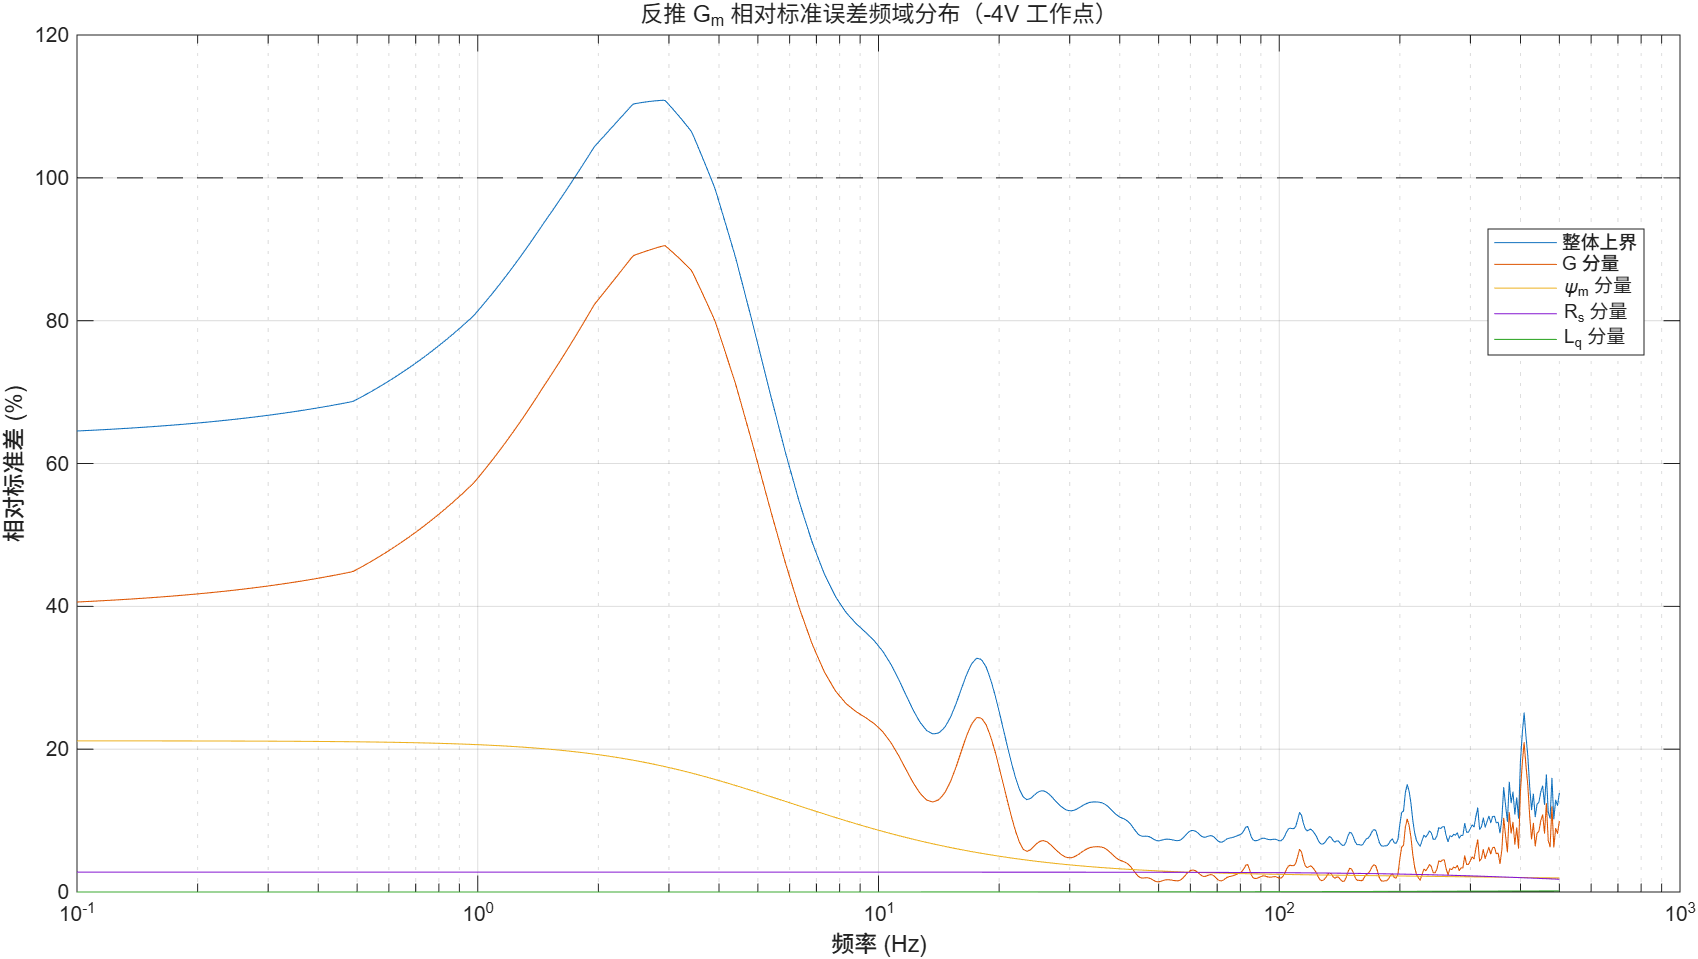
\includegraphics[width=\textwidth]
        {图片/相对标准误差频域分布曲线（-4V）.png}
        \caption{相对标准误差频域分布曲线（-4V）}
        \label{fig:相对标准误差频域分布曲线（-4V）}
    \end{minipage}
    \begin{minipage}{0.5\textwidth}
        \centering
        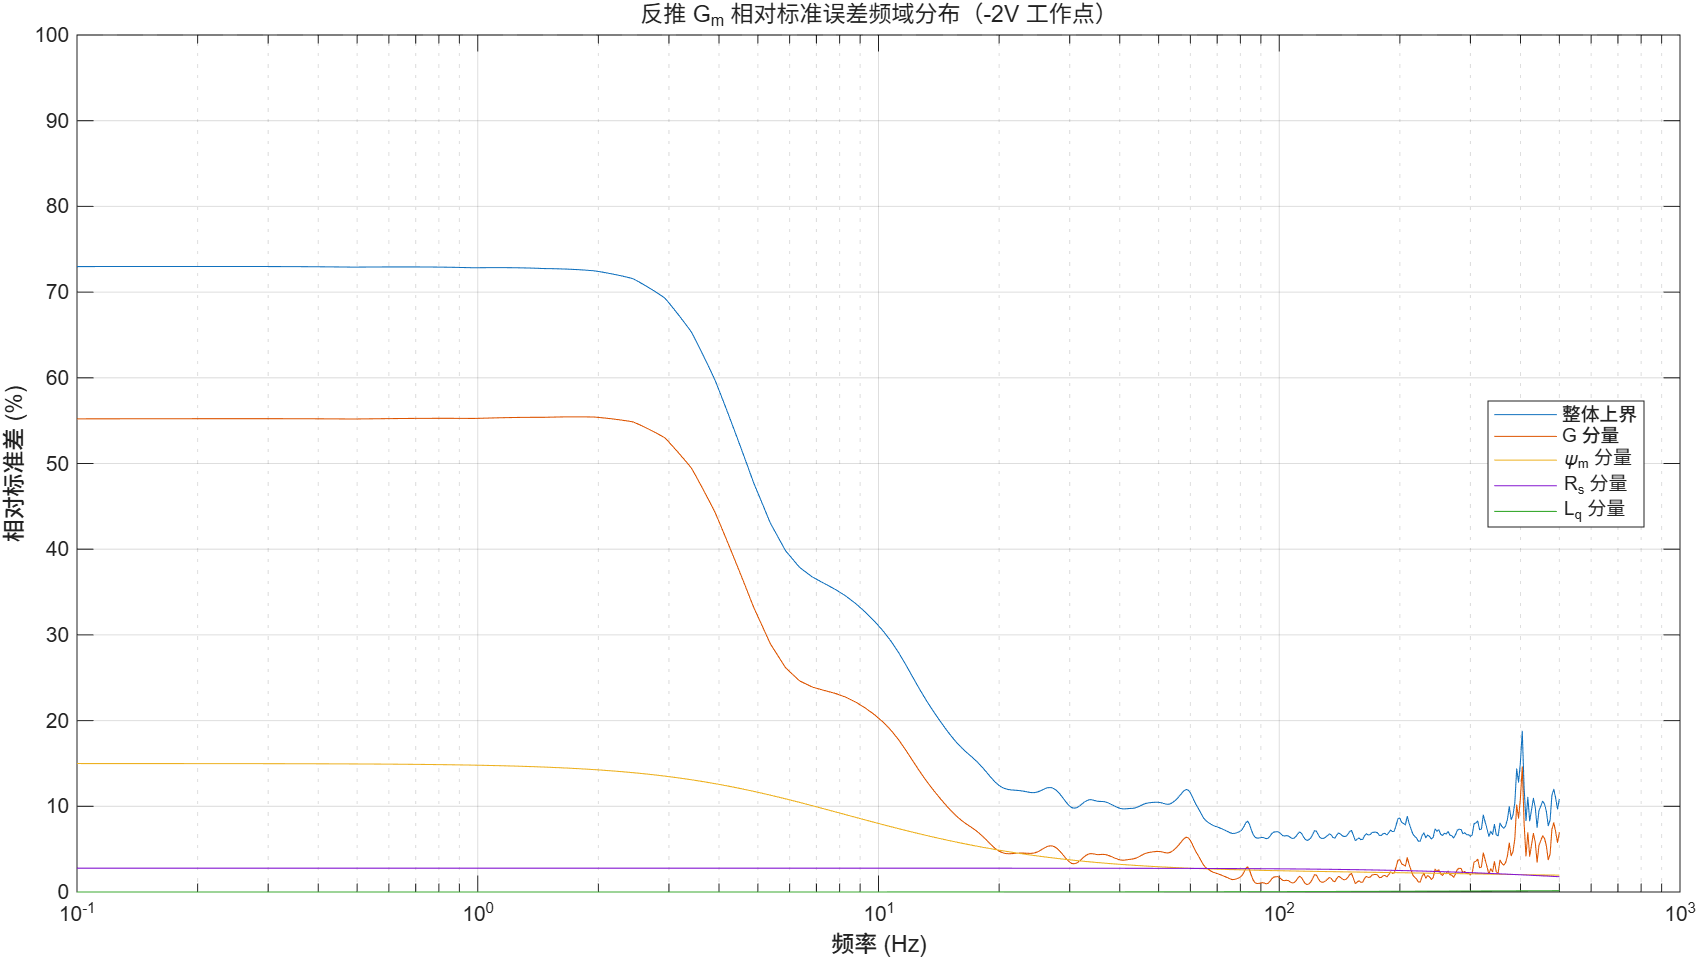
\includegraphics[width=\textwidth]
        {图片/相对标准误差频域分布曲线（-2V）.png}
        \caption{相对标准误差频域分布曲线（-2V）}
        \label{fig:相对标准误差频域分布曲线（-2V）}
    \end{minipage}
\end{figure}
\begin{figure}[H]
    \begin{minipage}{0.5\textwidth}
        \centering
        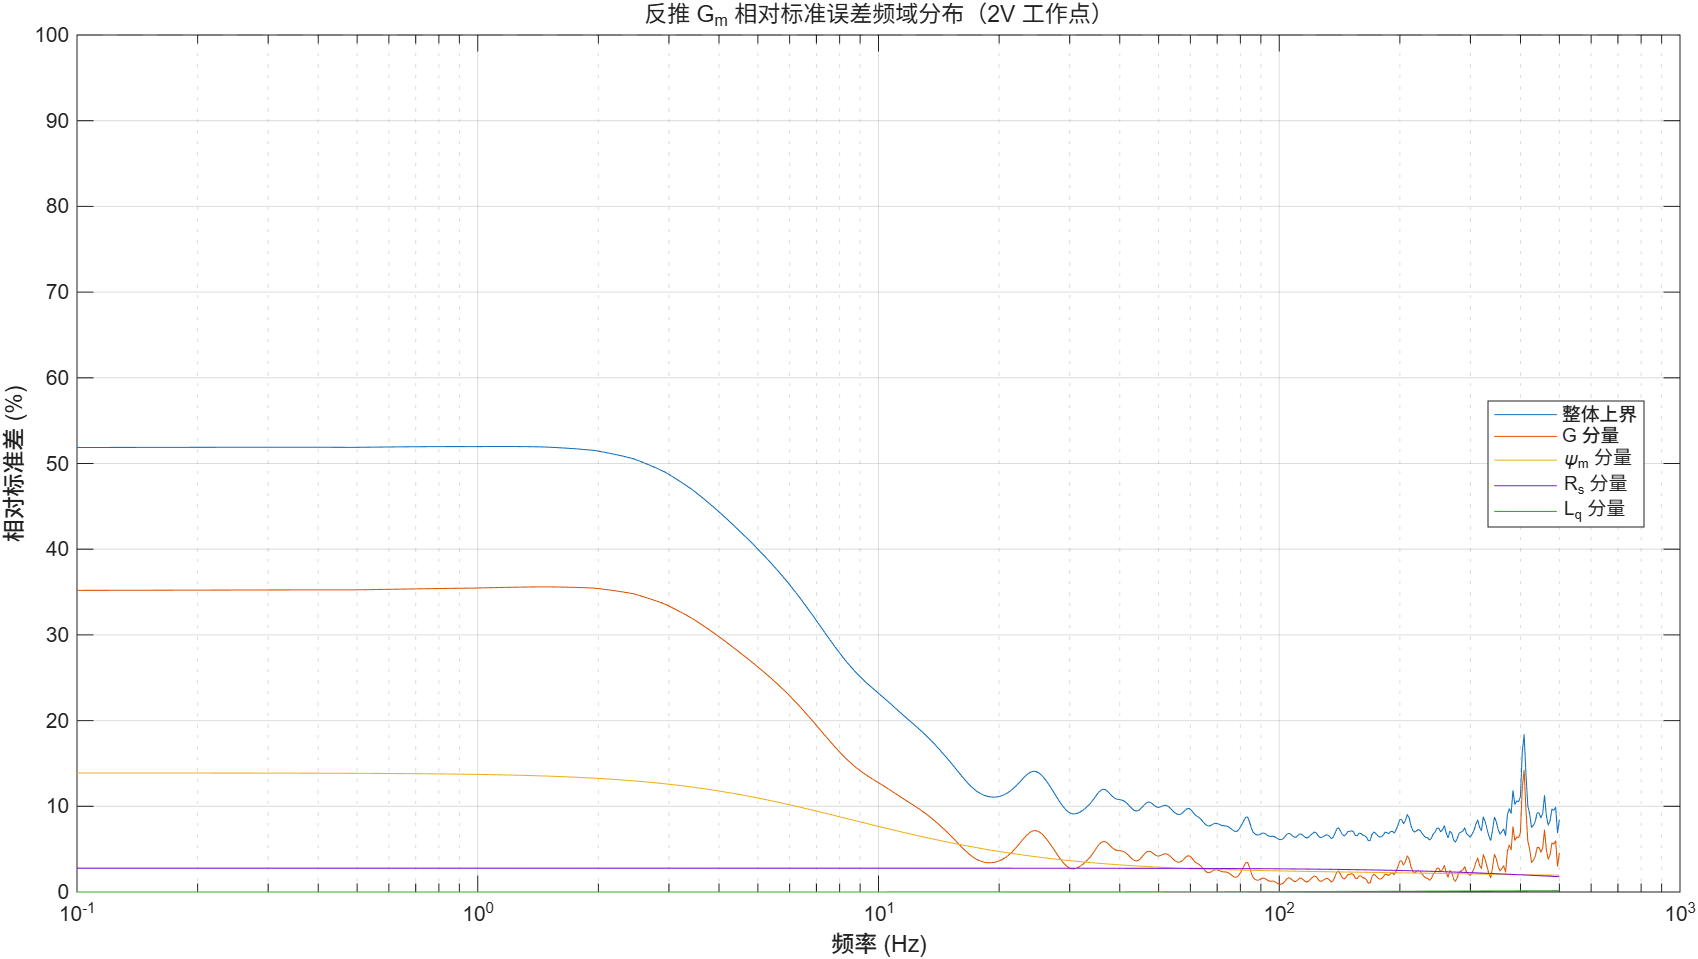
\includegraphics[width=\textwidth]
        {图片/相对标准误差频域分布曲线（2V）.png}
        \caption{相对标准误差频域分布曲线（2V）}
        \label{fig:相对标准误差频域分布曲线（2V）}
    \end{minipage}
    \begin{minipage}{0.5\textwidth}
        \centering
        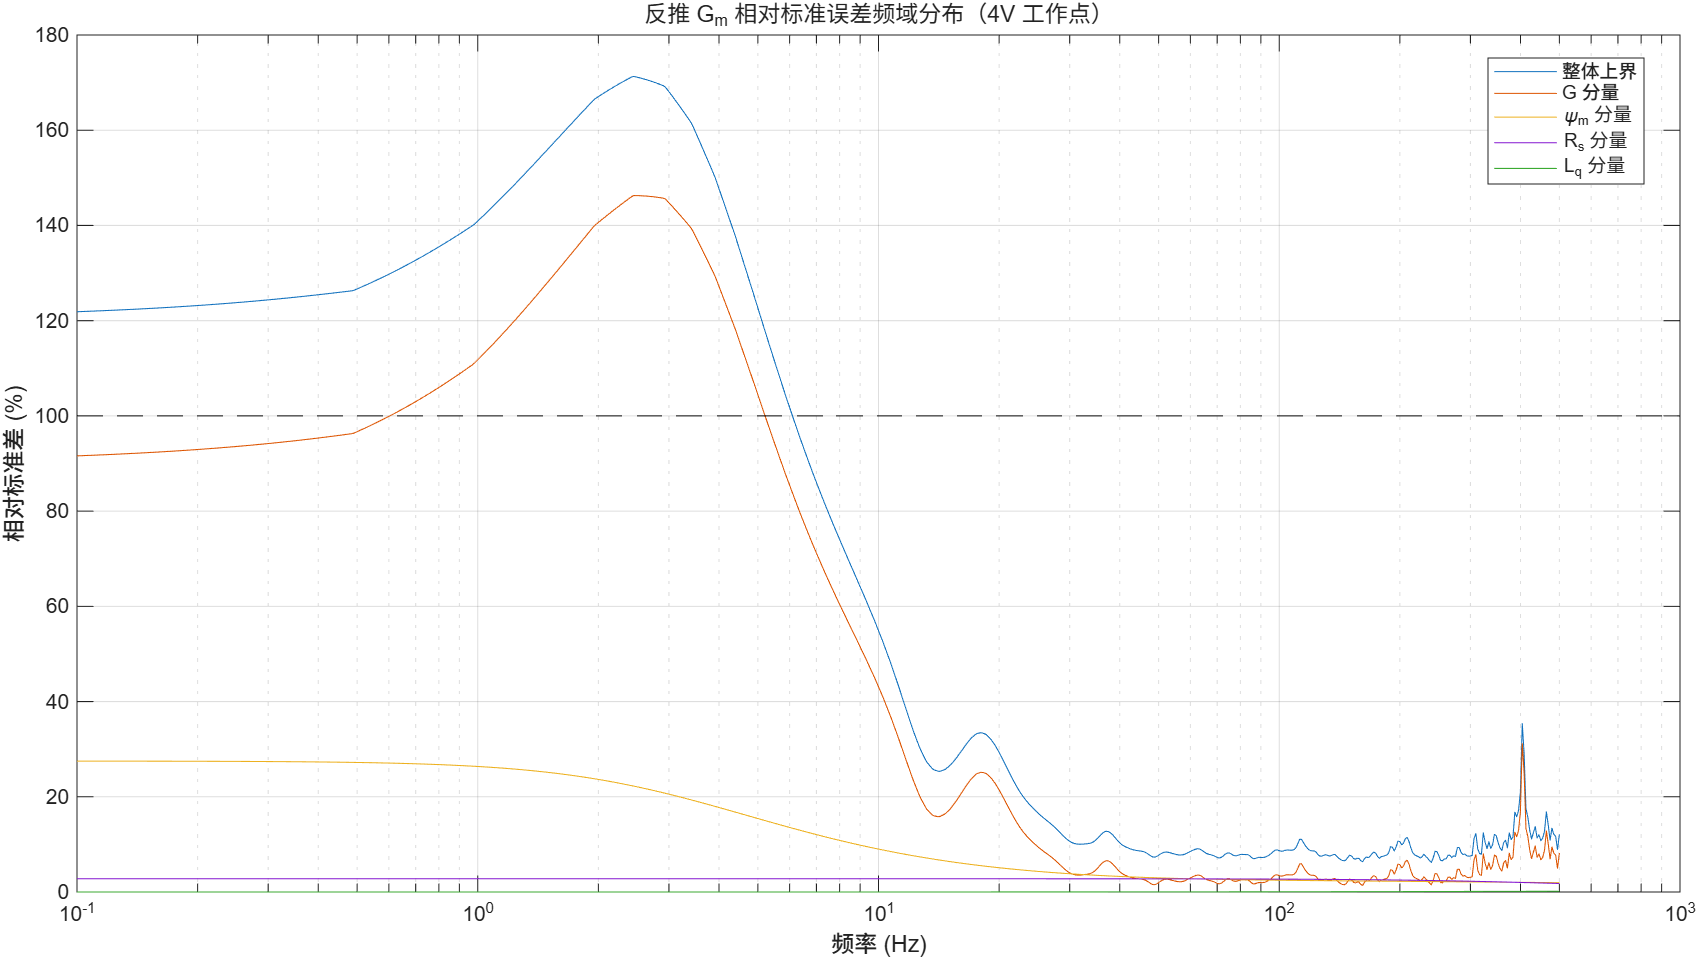
\includegraphics[width=\textwidth]
        {图片/相对标准误差频域分布曲线（4V）.png}
        \caption{相对标准误差频域分布曲线（4V）}
        \label{fig:相对标准误差频域分布曲线（4V）}
    \end{minipage}
\end{figure}

由图可知，±4V工作点在低频的相对误差超过100\%，即该处反推得到的\(G_{\mathrm{m}}\)误差已超过其本身，结果不可信；
±2V工作点相对误差均在75\%以下，其中核心频段（\(10\text{Hz}\sim 100\text{Hz}\)）约为20\%\(\sim\)30\%。
且±2V的误差随频率升高而降低，±4V在低频出现明显的破百峰。这解释了表\ref{tab:各工作点Gm辨识结果汇总}
中±4V工作点结果散布更大、而±2V工作点结果更一致的现象。据此，选取±2V工作点的平均结果作为参考模型，
排除反推结果不可信的±4V工作点。

最终得到极点[-1874.2, -38.7]、零点[-2629.4, 1961.8]、直流增益[18010]的机械传递函数：
\begin{equation}
    G_{\mathrm{m}}(s) = \frac{-18010s^2 - 1.202\times 10^7 s + 9.29\times 10^{10}}
    {71.12s^2 + 1.36\times 10^5 s + 5.158\times 10^6}
    \label{eq:Gm参考模型}
\end{equation}

值得说明的是，极低频段的辨识误差对闭环控制性能的影响较为有限，这是因为为了实现无差跟踪控制器含积分环节，
低频时开环增益趋于无穷，闭环传递函数在低频趋于1，因此辨识模型的低频辨识误差能够被控制器压制。
真正影响控制器设计的是核心频段10\(\sim\)100Hz的误差，该频段±2V工作点的相对误差为
20\%\(\sim\)30\%，还可以通过增大裕度来压制。±4V工作点在这部分的相对误差更高，故采用±2V工作点的辨识结果。

另外，如果想要较为准确地获取极低频段的辨识结果（主要是开环直流增益），可以尝试通过多点闭环直流增益（转速常数）测量，拟合出平均
闭环直流增益直接反推开环直流增益。实测发现，闭环直流增益最小二乘拟合后约67.4 rpm/V，
高于辨识模型隐含的约63.6 rpm/V，且观察到了明显的转速常数随工作点而升高的现象。
将修正后的开环直流增益代入模型后，开环与闭环验证均与实测明显不符。
推测原因有三个：其一是灵敏度函数\(S_{G}(\mathrm{j\omega})\)太大，转速常数的很小偏差都会在开环直流增益中引发
极大的偏离\footnote{直流处灵敏度函数\(S_G(\mathrm{j}0)=[1-\cfrac{\pi}{30}p\psi_{\mathrm{m}}G(0)]^{-1}\approx 22\)，
即转速常数（闭环直流增益）1\%的相对偏差经反推会被放大为开环直流增益约22\%的偏离。}；其二是电机本身的非线性因素较强，齿槽转矩严重，
在恒定电压激励下会因为齿槽转矩而发生周期性波动，难以准确计算
稳态转速和转速常数；其三是由于机械摩擦和逆变器死区导致测得的转速常数随激励电压而变化，使得用单一数值描述本身就缺乏合理性。
最终确定开环直流增益无法由闭环数据稳健反推，故保留辨识模型，并将极低频误差交由积分环节压制。

\subsubsection{辨识结果的开环验证}
根据\eqref{eq:Q轴电流-速度闭环传递函数表达式}，可以得到Q轴反电动势闭环传递函数：
\begin{equation*}
    G(s)=\cfrac{-3774 s^2 - 2.068\times10^6 s + 2.065\times 10^{10}}
    {2.298 s^3 + 7367 s^2 + 3.607\times 10^6 s +3.238\times 10^{8}}
\end{equation*}

由于电机的速度来源与对角度传感器的微分，微分噪声极大，因此在开环和后续的闭环验证中需要加入低通滤波器
\(F(z)=\cfrac{0.1}{1-0.9z^{-1}}\)
\footnote{辨识时不加入该滤波器，主要出于两方面考虑。其一，滤波器串联后辨识得到的是\(F(z)\times\text{ZOH}[G_{\mathrm{m}}(s)]\)的级联模型，
从中分离\(G_{\mathrm{m}}(s)\)需进行反卷积，会引入额外不确定性。其二，\(F(z)\)的极点\(z=0.9\)对应连续域频率远高于机械带宽，
Ho-Kalman辨识算法试图在全频段进行拟合，需分配额外阶次拟合该快动态，在有限数据长度下会削弱机械模态的估计精度。实测结果也表明，
加入\(F(z)\)尽管转速信号更加平滑，但辨识的拟合优度和幅相频相关系数均有下降，模型与实测波形的吻合程度也不及不加滤波器时。
因此采用分步策略——辨识时直接获取\(G_{\mathrm{m}}(s)\)，验证时在输出端串联\(F(z)\)实现物理模型与测量滤波的解耦。}。
此时系统框图变为：
\begin{figure}[H]
    \centering
    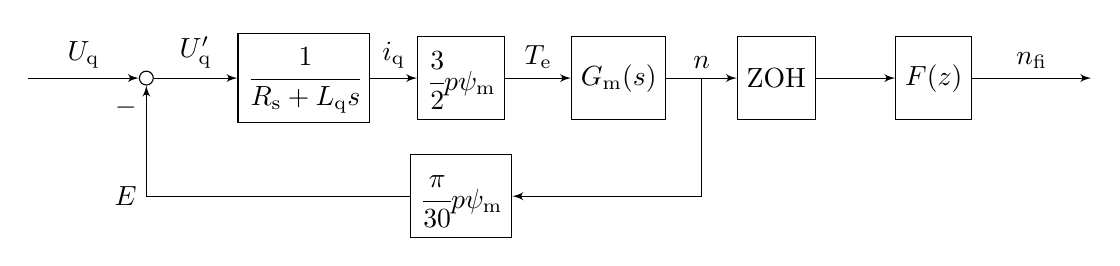
\begin{tikzpicture}[auto, node distance=2cm, >=latex']
        % 样式定义
        \tikzstyle{block} = [draw, rectangle, minimum height=3em, minimum width=1.5em, align=center]
        \tikzstyle{sum} = [draw, circle, node distance=1.5cm, minimum size=0.5em, inner sep=0pt]
        \tikzstyle{input} = [coordinate]
        \tikzstyle{output} = [coordinate]
        \tikzstyle{feedback} = [coordinate]

        % 放置节点
        \node [input, name=input] {};
        \node [sum, right of=input] (sum) {};
        \node [block, right of=sum] (RL) {\(\cfrac{1}{R_{\mathrm{s}}+L_{\mathrm{q}} s}\)};
        \node [block, right of=RL] (K) {\(\cfrac{3}{2}p\psi_{\mathrm{m}}\)};
        \node [block, right of=K] (Mech) {\(G_{\mathrm{m}}(s)\)};
        \node [block, right of=Mech] (ZOH) {ZOH};
        \node [block, right of=ZOH] (F) {\(F(z)\)};
        \node [output, right of=F] (output) {};
        \node [block, below of=K, node distance=1.5cm] (Kf) {\(\cfrac{\pi}{30}p\psi_{\mathrm{m}}\)};

        \draw [->] (input) -- node {\(U_{\mathrm{q}}\)} (sum);
        \draw [->] (sum) -- node {\(U_{\mathrm{q}}'\)} (RL);
        \draw [->] (RL) -- node {\(i_{\mathrm{q}}\)} (K);
        \draw [->] (K) -- node {\(T_{\mathrm{e}}\)} (Mech);
        \draw [->] (Mech) -- node [name=y] {\(n\)} (ZOH);
        \draw [->] (ZOH) -- node {} (F);
        \draw [->] (F) -- node {\(n_{\mathrm{fi}}\)} (output);
        \draw [->] (y) |- (Kf);
        \draw [->] (Kf) -| node[pos=0.9] {\(-\)} node [pos=0.5] {\(E\)} (sum);
    \end{tikzpicture}
    \caption{\(i_{\mathrm{d}}=0\)假设下的Q轴电流-速度系统框图（带低通滤波器）}
    \label{fig:Q轴电流-速度系统框图（带低通滤波器）}
\end{figure}

因此实际闭环传递函数应为使用零阶保持器离散化后与离散低通滤波器\(F(z)\)相乘的结果：
\begin{equation*}
    G(z)=\cfrac{0.3297 z^{-1} + 1.85 z^{-2} - 0.1351 z^{-3}}
    {1- 1.832 z^{-1} + 1.108 z^{-2} - 0.2565z^ {-3} + 0.0134z^{-4}}
\end{equation*}

选用幅值为±5V的方波信号作为激励信号，输入到\(U_{\mathrm{q}}\)，同时进行D轴闭环\(i_{\mathrm{d}}^*=0\)，在电机空载的情况下记录电机的转速响应。
但首先仍需要考虑\(i_{\mathrm{d}}=0\)理想条件是否满足。

施加正向方波时，考虑\(i_{\mathrm{d}}=0\)的理想化假设和\(i_{\mathrm{d}}\ne 0\)的实际情况，分析反电动势和电磁转矩波形如下图所示。
\begin{figure}[H]
    \begin{minipage}{0.5\textwidth}
        \centering
        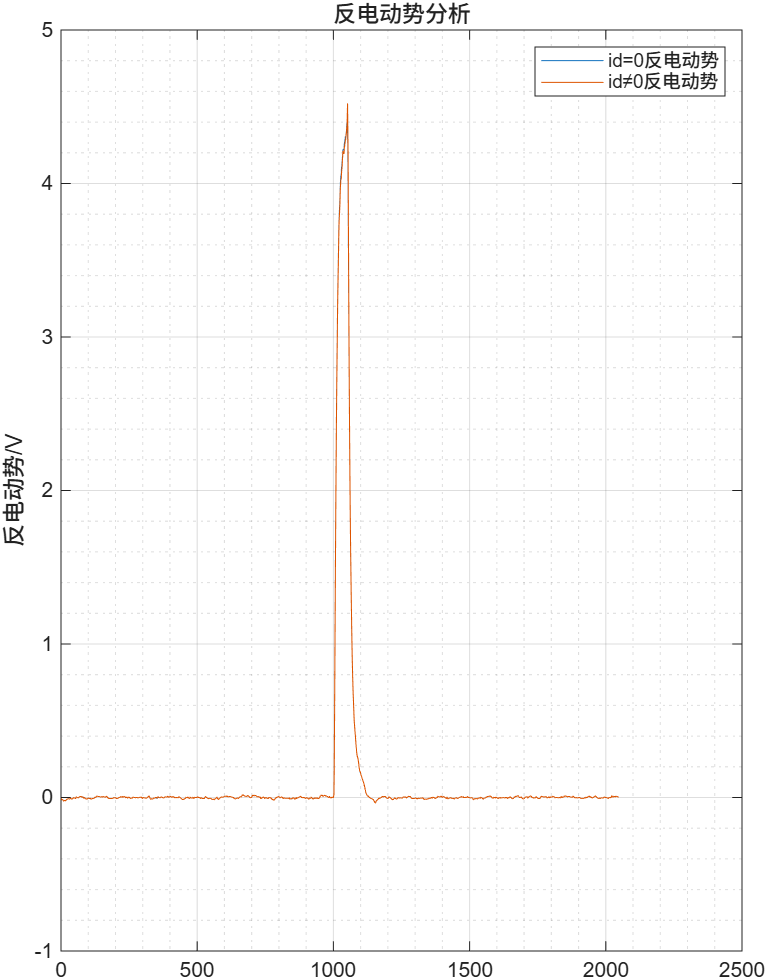
\includegraphics[width=\textwidth]  
        {图片/速度环正向方波反电动势对比.png}
        \caption{速度环正向方波反电动势对比}
    \end{minipage}
    \begin{minipage}{0.5\textwidth}
        \centering
        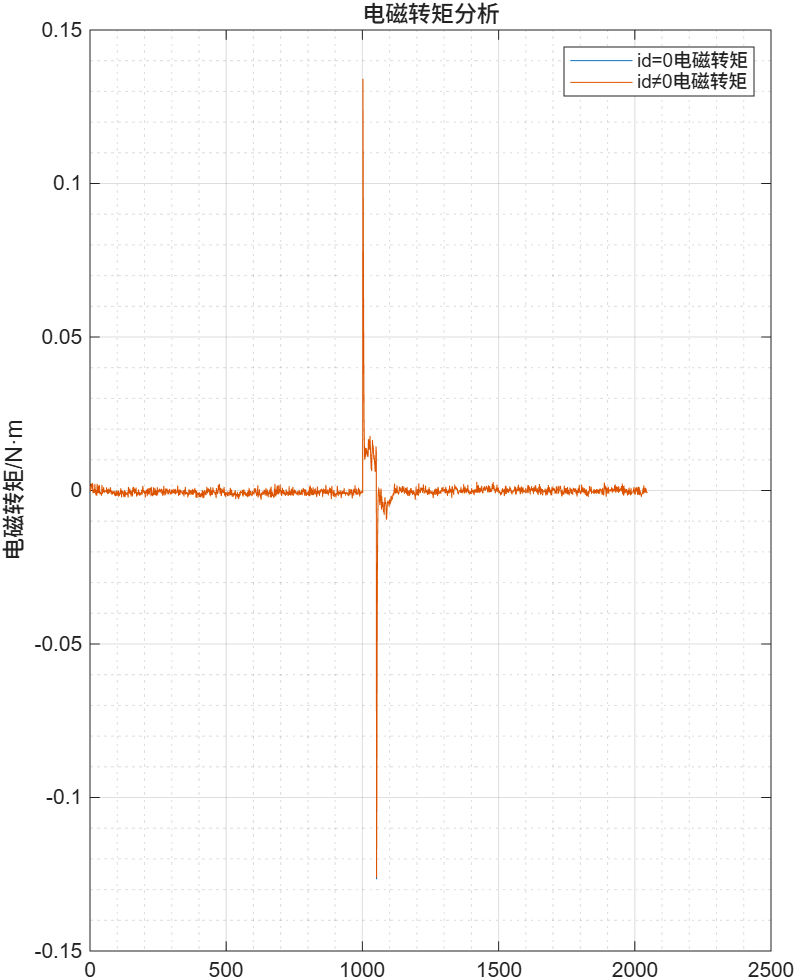
\includegraphics[width=\textwidth]
        {图片/速度环正向方波电磁转矩对比.png}
        \caption{速度环正向方波电磁转矩对比}
    \end{minipage}
    \label{fig:速度环正向方波理想id与实际id对比}
\end{figure}

分析可得反电动势相关系数99.99988\%，拟合优度99.84557\%；电磁转矩相关系数100.00000\%，拟合优度99.97289\%为极高水平，\(i_{\mathrm{d}}=0\)的
理想化假设可以认为是遵守的。此时仿真和实测的转速波形如下图所示。
\begin{figure}[H]
    \centering
    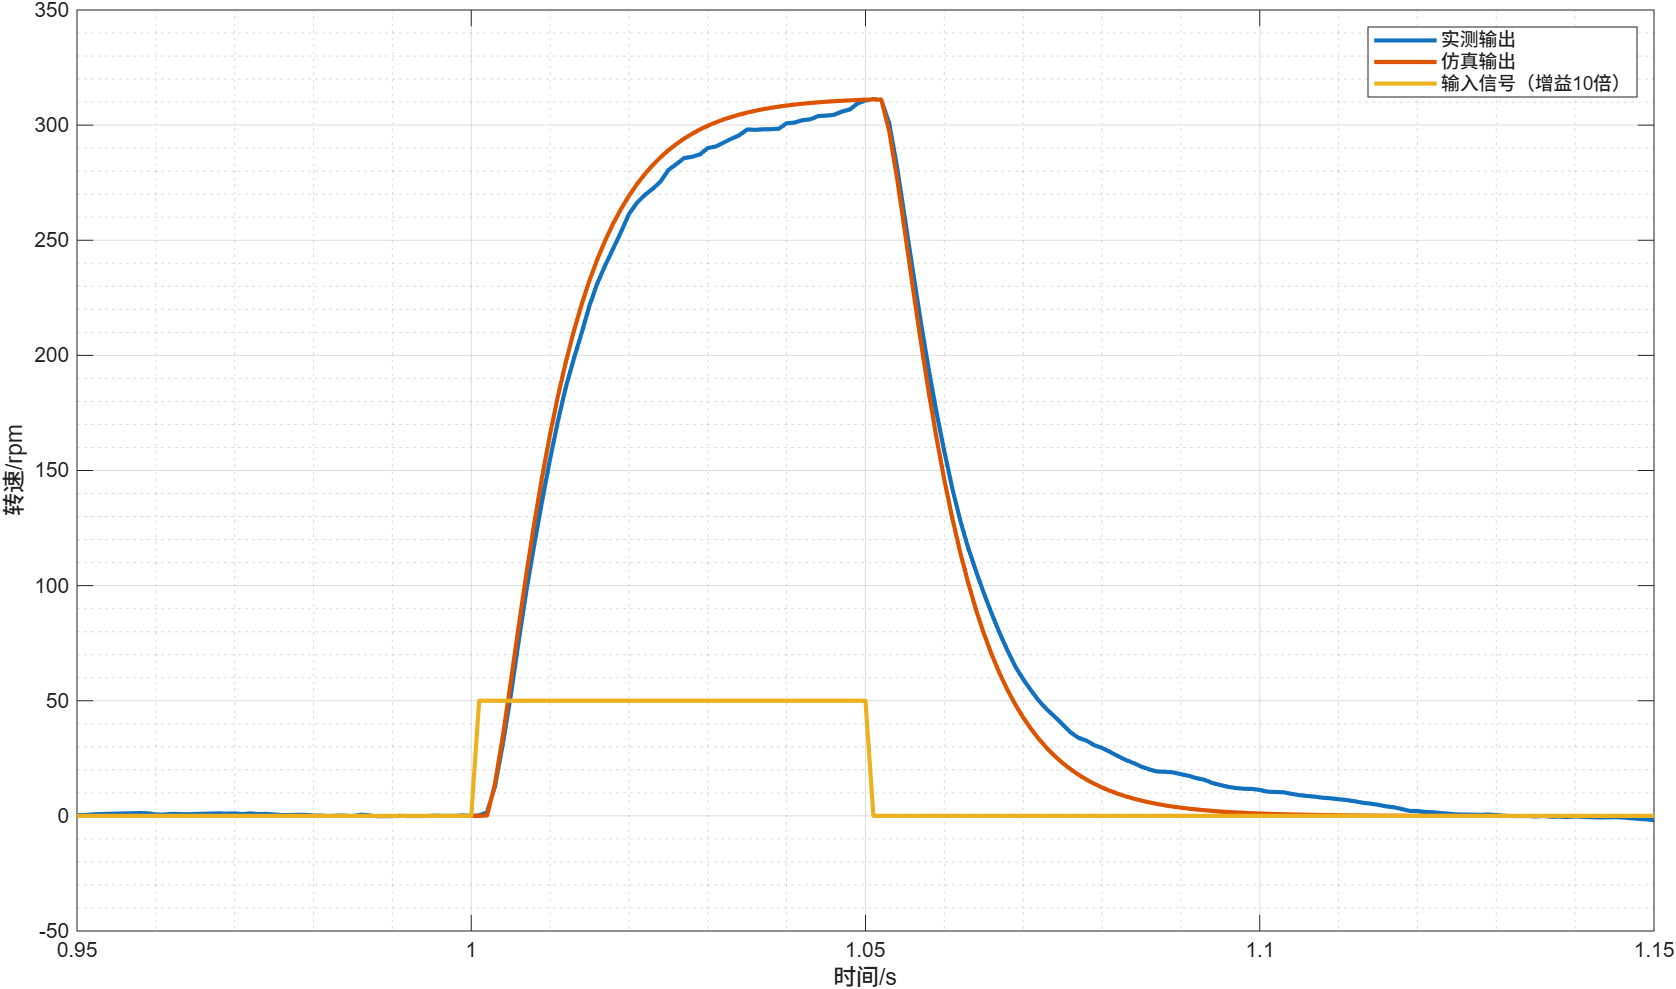
\includegraphics[width=0.6\textwidth]
    {图片/速度环正向方波转速对比.png}
    \caption{速度环正向方波转速对比}
    \label{fig:速度环正向方波转速对比}
\end{figure}

两个时域波形的相关系数99.85915\%，拟合优度93.11630\%。

负向方波作用下电动势和电磁转矩波形如下图所示。
\begin{figure}[H]
    \begin{minipage}{0.5\textwidth}
        \centering
        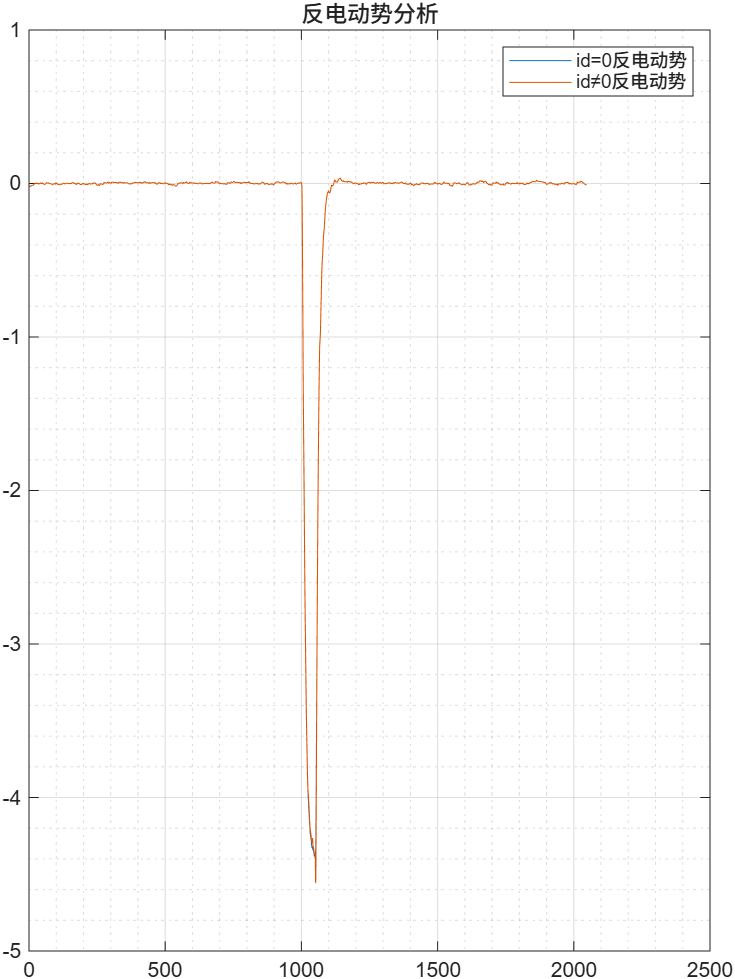
\includegraphics[width=\textwidth]
        {图片/速度环负向方波反电动势对比.png}
        \caption{速度环负向方波反电动势对比}
    \end{minipage}
    \begin{minipage}{0.5\textwidth}
        \centering
        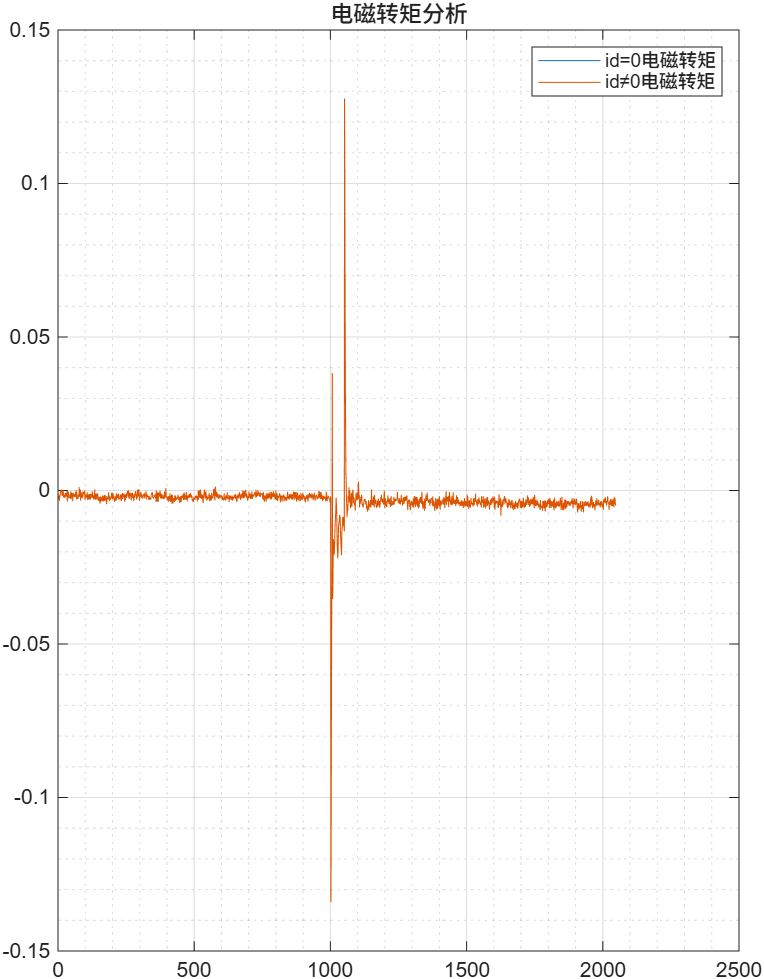
\includegraphics[width=\textwidth]
        {图片/速度环负向方波电磁转矩对比.png}
        \caption{速度环负向方波电磁转矩对比}
    \end{minipage}
    \label{fig:速度环负向方波理想id与实际id对比}
\end{figure}

分析可得反电动势相关系数99.99990\%，拟合优度99.84985\%；电磁转矩相关系数99.99999\%，拟合优度99.95191\%为极高水平，
同样遵守\(i_{\mathrm{d}}=0\)的理想化假设。此时仿真和实测的转速波形如下图所示。
\begin{figure}[H]
    \centering
    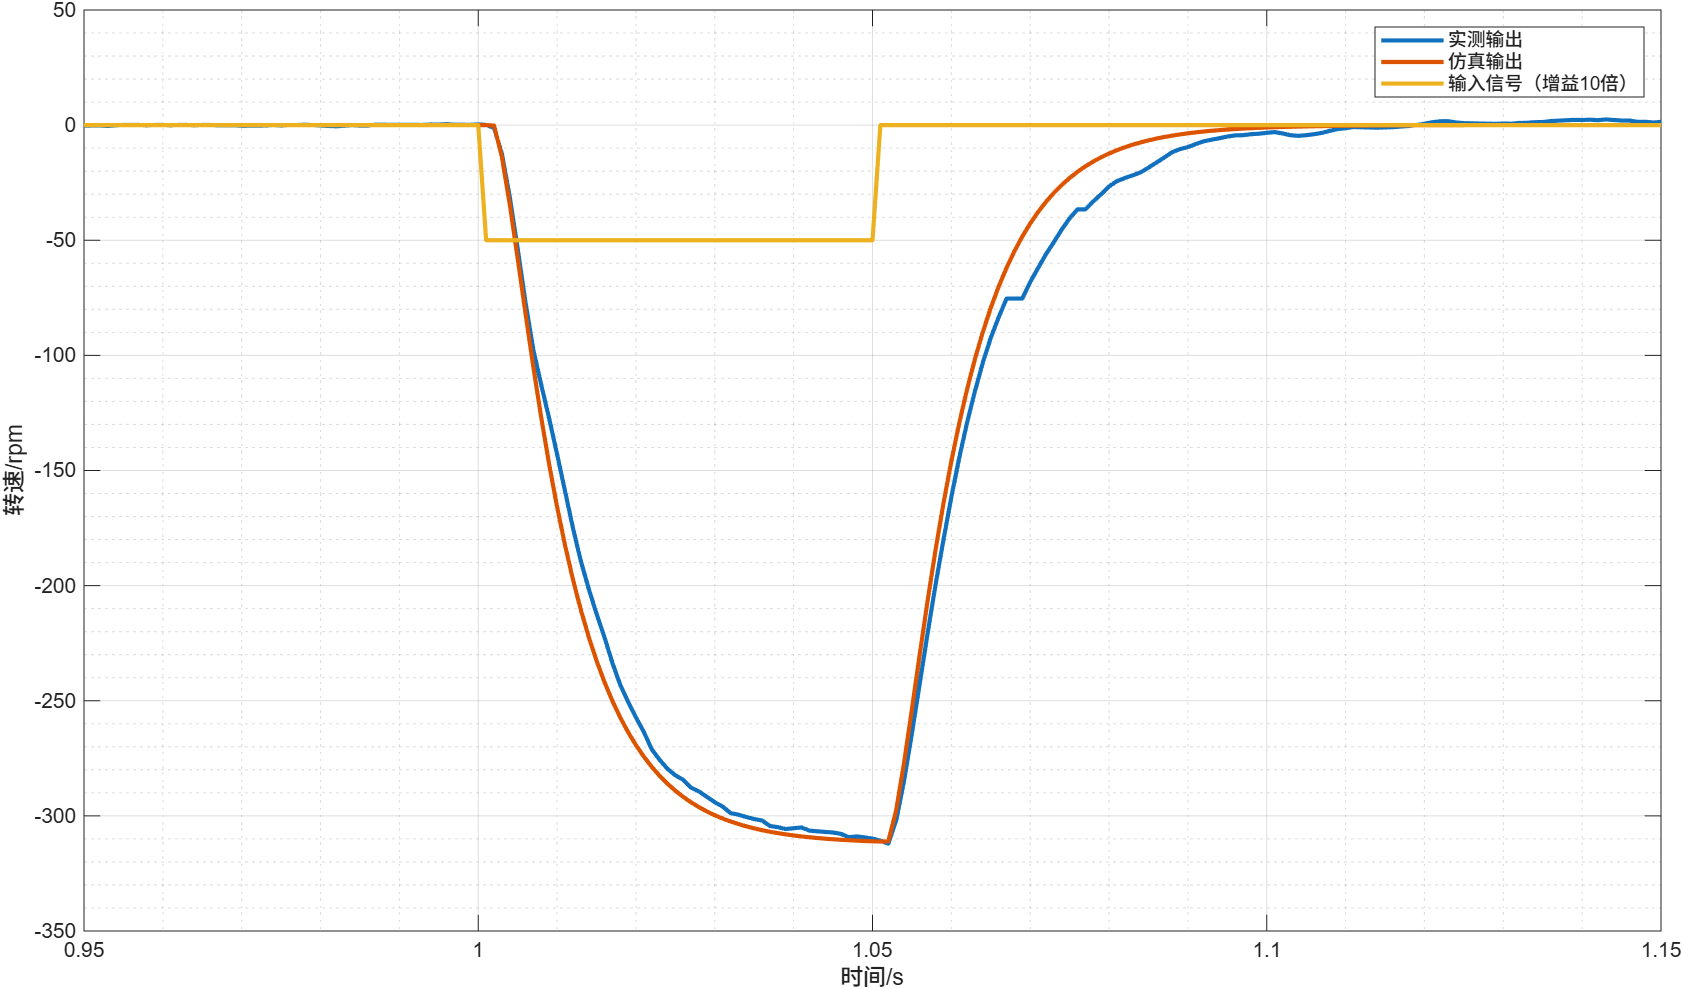
\includegraphics[width=0.6\textwidth]
    {图片/速度环负向方波转速对比.png}
    \caption{速度环负向方波转速对比}
    \label{fig:速度环负向方波转速对比}
\end{figure}

两个时域波形的相关系数99.92870\%，拟合优度95.71185\%。

据图\ref{fig:速度环正向方波转速对比}和图\ref{fig:速度环负向方波转速对比}可知，在暂态响应段仿真和实测波形高度一致。
而接近稳态时角加速度趋零，惯性力矩\(J\cfrac{\dd n}{\dd t}\)随之消失，齿槽转矩作为周期性扰动在速度波形上显现出来，
但振荡的均值与仿真波形的均值一致。说明建立的系统模型能够较为准确地解释电机的响应，但对非线性的齿槽转矩确实无法实现建模。

\subsection{速度环频域矫正控制器设计与闭环验证}
\subsubsection{速度环被控对象建模}
速度环频域矫正控制器仍采用与电流环相同的带积分环节超前校正结构，但被控对象不同于电流环的纯RL电路，
需要考虑反电动势反馈路径的物理存在。

在\ref{sec:电流环频域矫正控制器设计}中Q轴电流环控制器\(C_{\mathrm{q}}(s)\)按被控对象为纯RL电路模型\(\cfrac{1}{R_{\mathrm{s}}+L_{\mathrm{q}} s}\)设计，
并通过方波短脉冲测试（0.33ms内转速不发生明显变化）验证了该设计的有效性。但在速度环闭环控制中，转速\(n\)在秒级时间内大幅变化，
反电动势\(\omega_{\mathrm{e}}\psi_{\mathrm{m}}\)随转速动态变化，不再能视为常数扰动。此时从电流给定\(i_{\mathrm{q}}^*\)到转速\(n\)的物理被控对象包含反电动势反馈路径，
其传递函数为：

\begin{equation*}
    G_{\text{speed}}(s)=\cfrac{n(s)}{i_{\mathrm{q}}^*(s)}=
    \cfrac{C_{\mathrm{q}}(s)\times\cfrac{1}{R_{\mathrm{s}}+L_{\mathrm{q}} s}\times\cfrac{3}{2}p\psi_{\mathrm{m}}\times G_{\mathrm{m}}(s)}
    {1+\cfrac{\pi}{30}p\psi_{\mathrm{m}}\times\cfrac{1}{R_{\mathrm{s}}+L_{\mathrm{q}} s}\times\cfrac{3}{2}p\psi_{\mathrm{m}}\times G_{\mathrm{m}}(s)
    +C_{\mathrm{q}}(s)\times\cfrac{1}{R_{\mathrm{s}}+L_{\mathrm{q}} s}}
\end{equation*}

代入平均模型\eqref{eq:Gm参考模型}，进行ZOH按照采样频率1kHz离散化后经过低通滤波器\(F(z)=\cfrac{0.1}{1-0.9z^{-1}}\)，
可得等价离散化被控对象模型：
\begin{equation*}
    G_{\mathrm{s}}(z)=
    \cfrac{
        \begin{array}[t]{@{}l@{}}
            3.389 z^{-1} + 0.2123 z^{-2} - 14.06 z^{-3} + 15.6 z^{-4} - 6.191 z^{-5} + 1.179 z^{-6} \\
            - 0.1164 z^{-7} + 0.005744 z^{-8} - 0.0001118 z^{-9} + 1.374\times 10^{-9}z^{-10} - 1.141\times 10^{-19}z^{-11}
        \end{array}}
        {
        \begin{array}[t]{@{}l@{}}
            1 - 4.386 z^{-1} + 7.816 z^{-2} - 7.259 z^{-3} + 3.775 z^{-4} - 1.12 z^{-5} + 0.193 z^{-6} \\
            - 0.01891 z^{-7} + 0.0009637 z^{-8} - 1.967\times 10^{-5} z^{-9} + 1.963\times 10^{-10} z^{-10} - 7.451\times 10^{-16} z^{-11} \\
            + 6.191\times 10^{-26}z^{-12}
        \end{array}}
\end{equation*}

此时的双闭环控制系统框图如下图所示：

\begin{figure}[H]
    \centering
    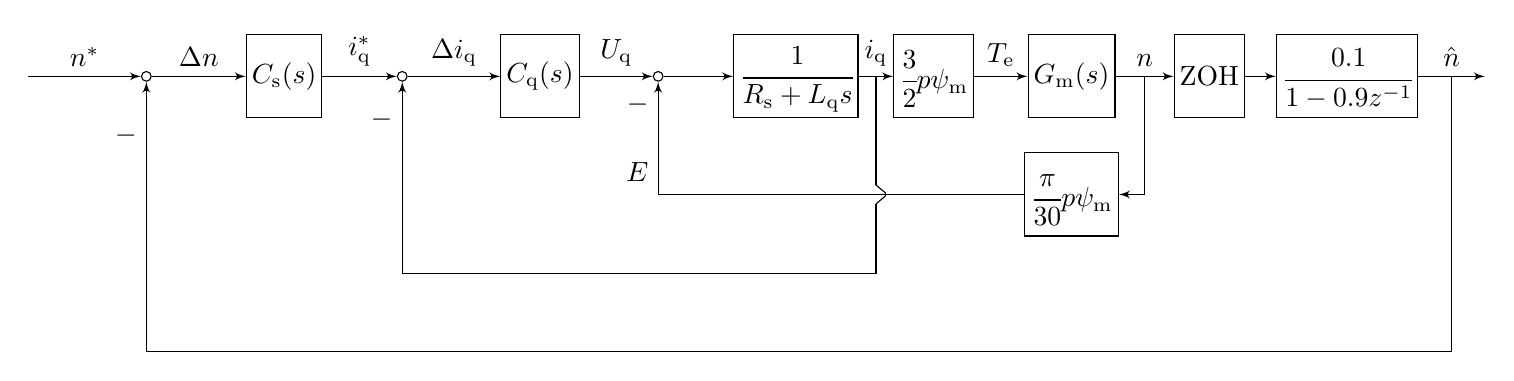
\begin{tikzpicture}[auto, node distance=1.75cm, >=latex']
        % 样式定义
        \tikzstyle{block} = [draw, rectangle, minimum height=3em, minimum width=1.8em, align=center, inner sep=2pt]
        \tikzstyle{sum} = [draw, circle, node distance=1.5cm, minimum size=0.35em, inner sep=0pt]
        \tikzstyle{input} = [coordinate]
        \tikzstyle{output} = [coordinate]
        \tikzstyle{feedback} = [coordinate]

        % 放置节点
        \node [input, name=input] {};
        \node [sum, right of=input] (sum1) {};
        \node [block, right of=sum1] (Cs) {\(C_{\mathrm{s}}(s)\)};
        \node [sum, right of=Cs] (sum2) {};
        \node [block, right of=sum2] (Cq) {\(C_{\mathrm{q}}(s)\)};
        \node [sum, right of=Cq] (sum) {};
        \node [block, right of=sum] (RL) {\(\cfrac{1}{R_{\mathrm{s}}+L_{\mathrm{q}} s}\)};
        \node [block, right of=RL] (K) {\(\cfrac{3}{2}p\psi_{\mathrm{m}}\)};
        \node [block, right of=K] (Mech) {\(G_{\mathrm{m}}(s)\)};
        \node [block, right of=Mech] (ZOH) {ZOH};
        \node [block, right of=ZOH] (Filter) {\(\cfrac{0.1}{1-0.9z^{-1}}\)};
        \node [output, right of=Filter] (output) {};
        \node [block, below of=Mech, node distance=1.5cm] (Kf) {\(\cfrac{\pi}{30}p\psi_{\mathrm{m}}\)};
        \node [feedback, below of=sum, node distance=3.5cm] (F) {};
        \node [feedback, below of=Cq,node distance=2.5cm] (Fb) {};

        \draw [->] (input) -- node {\(n^*\)} (sum1);
        \draw [->] (sum1) -- node {\(\Delta n\)} (Cs);
        \draw [->] (Cs) -- node {\(i_{\mathrm{q}}^*\)} (sum2);
        \draw [->] (sum2) -- node {\(\Delta i_{\mathrm{q}}\)} (Cq);
        \draw [->] (Cq) -- node {\(U_{\mathrm{q}}\)} (sum);
        \draw [->] (sum) -- node {} (RL);
        \draw [->] (RL) -- node [name=iq] {\(i_{\mathrm{q}}\)} (K);
        \draw [->] (K) -- node {\(T_{\mathrm{e}}\)} (Mech);
        \draw [->] (Mech) -- node [name=y] {\(n\)} (ZOH);
        \draw [->] (ZOH) -- node {} (Filter);
        \draw [->] (Filter) -- node [name=y_fi] {\(\hat{n}\)} (output);
        % 反电动势反馈
        \draw [->] (y) |- (Kf);
        \draw [->] (Kf) -| node[pos=0.9] {\(-\)} node [pos=0.6] {\(E\)} (sum);
        % i_{\mathrm{q}}反馈：在交叉点处加桥接小弧（跳线），与反电动势线路交叉但不连接
        \coordinate (cross) at (iq |- Kf);
        \coordinate (jT) at ([yshift=0.12cm] cross);
        \coordinate (jB) at ([yshift=-0.12cm] cross);
        \draw [-] (iq) -- (jT);
        \draw [-] (jT) -- ++(0.12, -0.1) -- ++(0, -0.04) -- ++(-0.12, -0.1);
        \draw [-] (jB) |- (Fb);
        \draw [->] (Fb) -| node[pos=0.9] {\(-\)} node [pos=0.6] {} (sum2);
        \draw [-] (y_fi) |- (F);
        \draw [->] (F) -| node[pos=0.9] {\(-\)} node [pos=0.6] {} (sum1);
    \end{tikzpicture}
    \caption{Q轴双闭环控制系统框图}
    \label{fig:Q轴双闭环控制系统框图}
\end{figure}

\subsubsection{控制器设计与闭环验证}
为了实现无静差跟踪，在被控对象前串入积分环节。构成等价被控对象，开环伯德图如下图所示。
\begin{figure}[H]
    \centering
    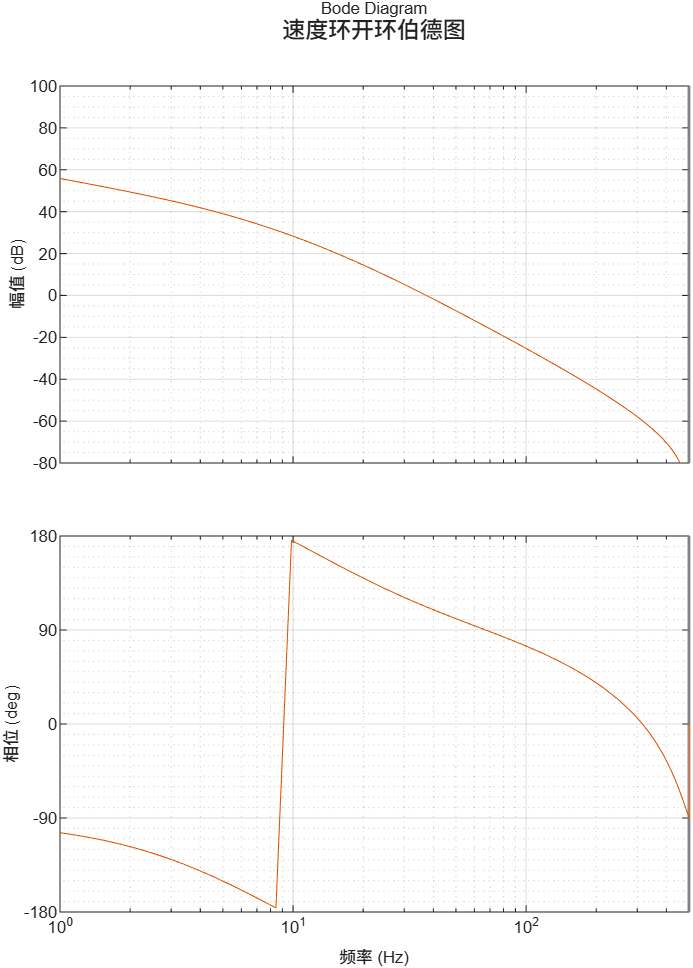
\includegraphics[width=0.5\textwidth]
    {图片/带积分环节的速度环等价被控对象开环频率特性.png}
    \caption{带积分环节的速度环等价被控对象开环频率特性}
\end{figure}

与电流环控制器一样，采用一阶超前校正控制\(C_{\mathrm{s}}(s)=K\cfrac{Ts+1}{\alpha Ts+1}\)，开环截止频率设定为13Hz，
以不低于40°的相位裕度为目标，在13Hz处提供最多65°的相位补偿，可以计算得到：
\begin{equation*}
    \begin{cases}
        \alpha = \cfrac{1-\sin(65°)}{1+\sin(65°)}=0.0491\\
        T = \cfrac{1}{2\pi\times 12\sqrt{\alpha}} = 0.0552
    \end{cases}
\end{equation*}

最后根据等价被控对象在12Hz处的增益，调整放大系数K，最终可得带积分的速度环超前控制器：
\begin{equation*}
    C_{\mathrm{s}}(s)=\cfrac{0.0008946s+0.0162}{0.002714s^2+s}
\end{equation*}

使用双线性变换离散化后得到：
\begin{equation*}
    C_{\mathrm{s}}(z)=\cfrac{0.0001404+2.52\times 10^{-6}z^{-1}-0.0001379z^{-2}}{1-1.6889z^{-1}+0.6889z^{-2}}
\end{equation*}

经过超前控制后的开环频率特性和闭环频率特性如下图所示。
\begin{figure}[H]
    \centering
    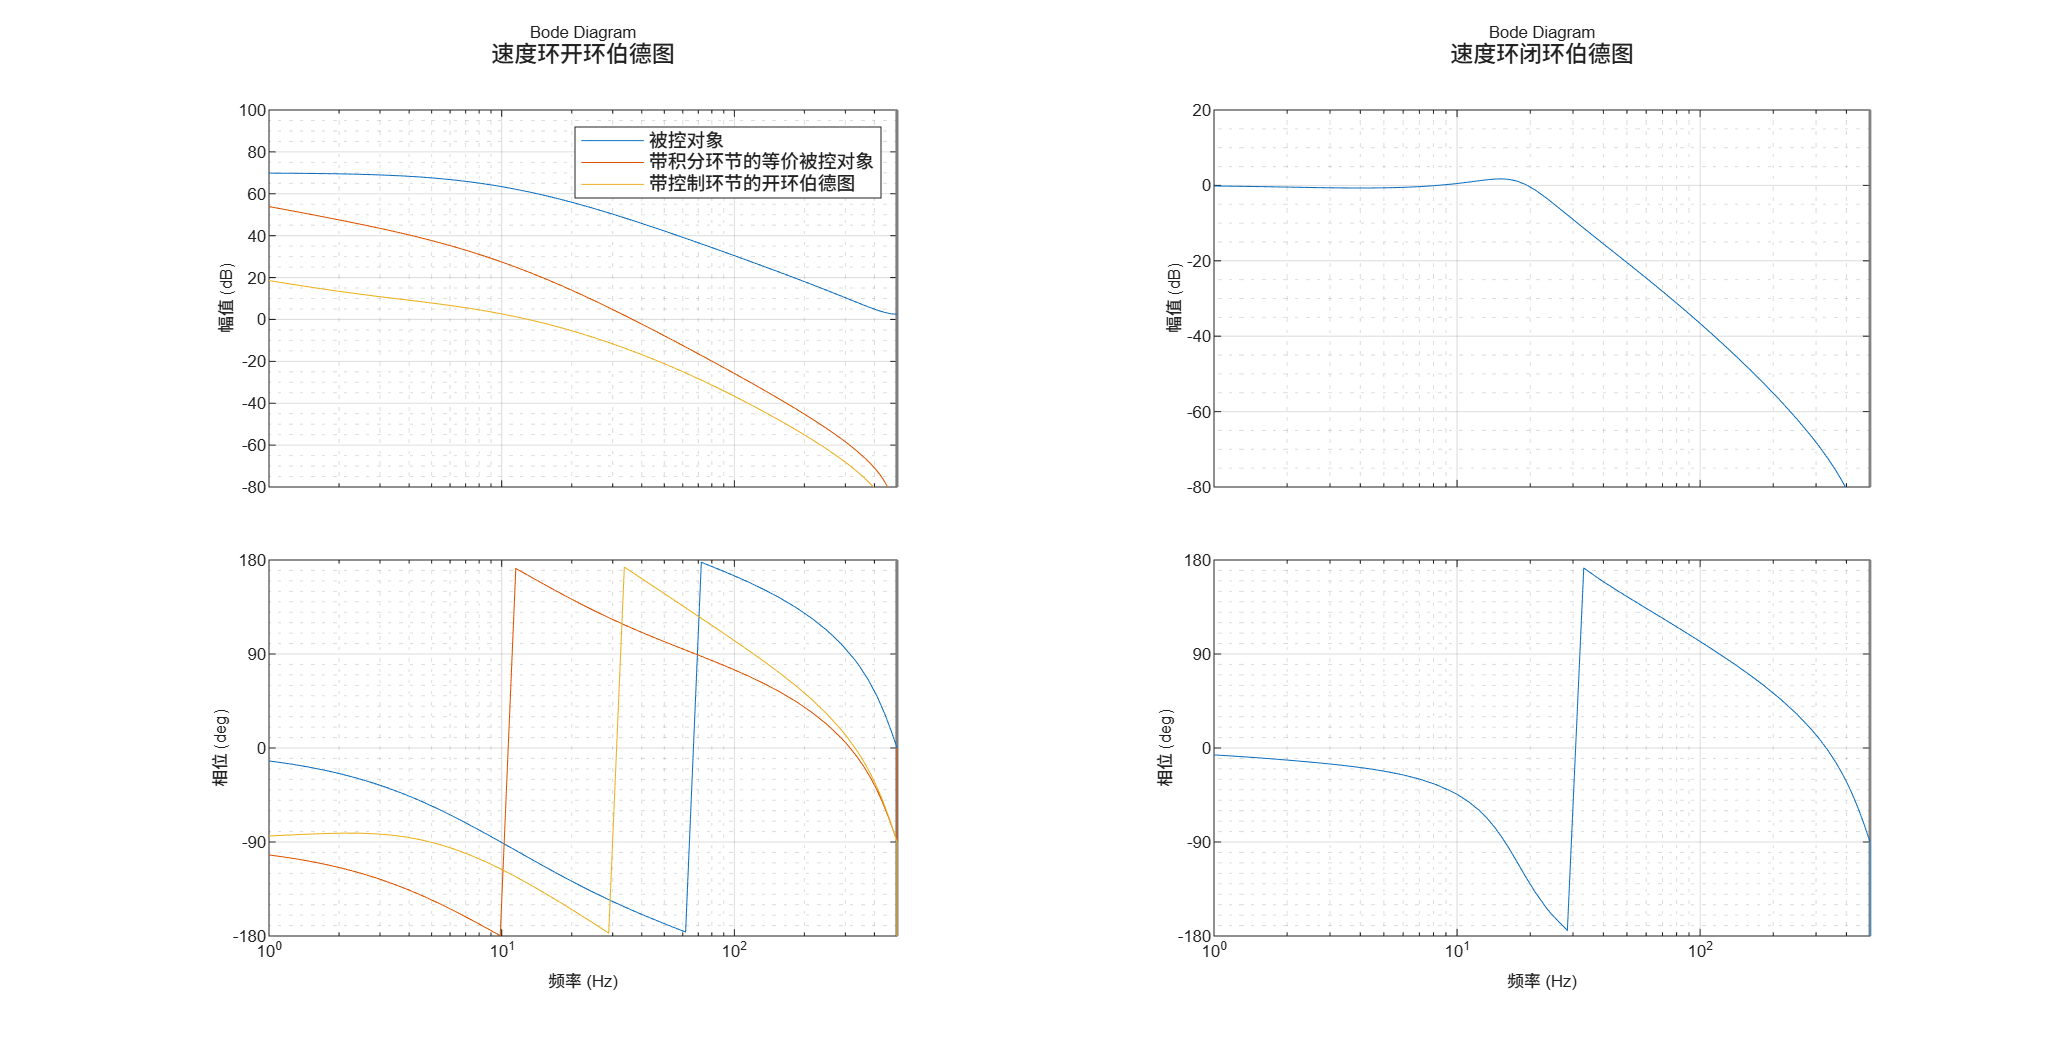
\includegraphics[width=\textwidth]
    {图片/速度环开-闭环频率特性.png}
    \caption{速度环开-闭环频率特性}
\end{figure}

矫正后，速度环的开环截止频率13Hz，相位裕度50.21128°满足设计要求。相位穿越频率30.14228Hz，
幅值裕度11.75946dB，闭环带宽22.95915Hz。闭环前后的单位阶跃响应如下图所示。
\begin{figure}[H]
    \centering
    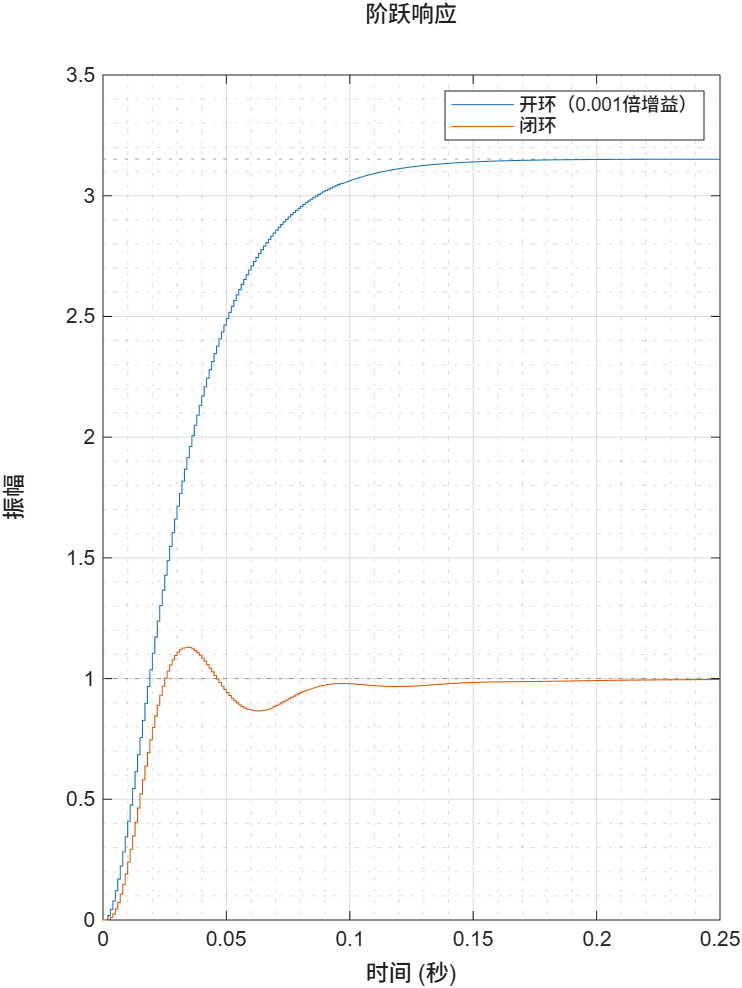
\includegraphics[width=0.5\textwidth]
    {图片/速度环开-闭环单位阶跃响应对比.png}
    \caption{速度环开-闭环单位阶跃响应对比}
\end{figure}

可以发现，通过带积分环节的超前校正控制器，使得能够无差跟踪给定信号，超调量13\%，调节时间为0.142s，用一定的超调
换来了极快的响应速度。接下来考虑以±150rpm的方波速度给定信号（持续500个采样周期）进行测试，以评估实际系统响应和
建模准确性，结果如下图所示。
\begin{figure}[H]
    \begin{minipage}{0.5\textwidth}
        \centering
        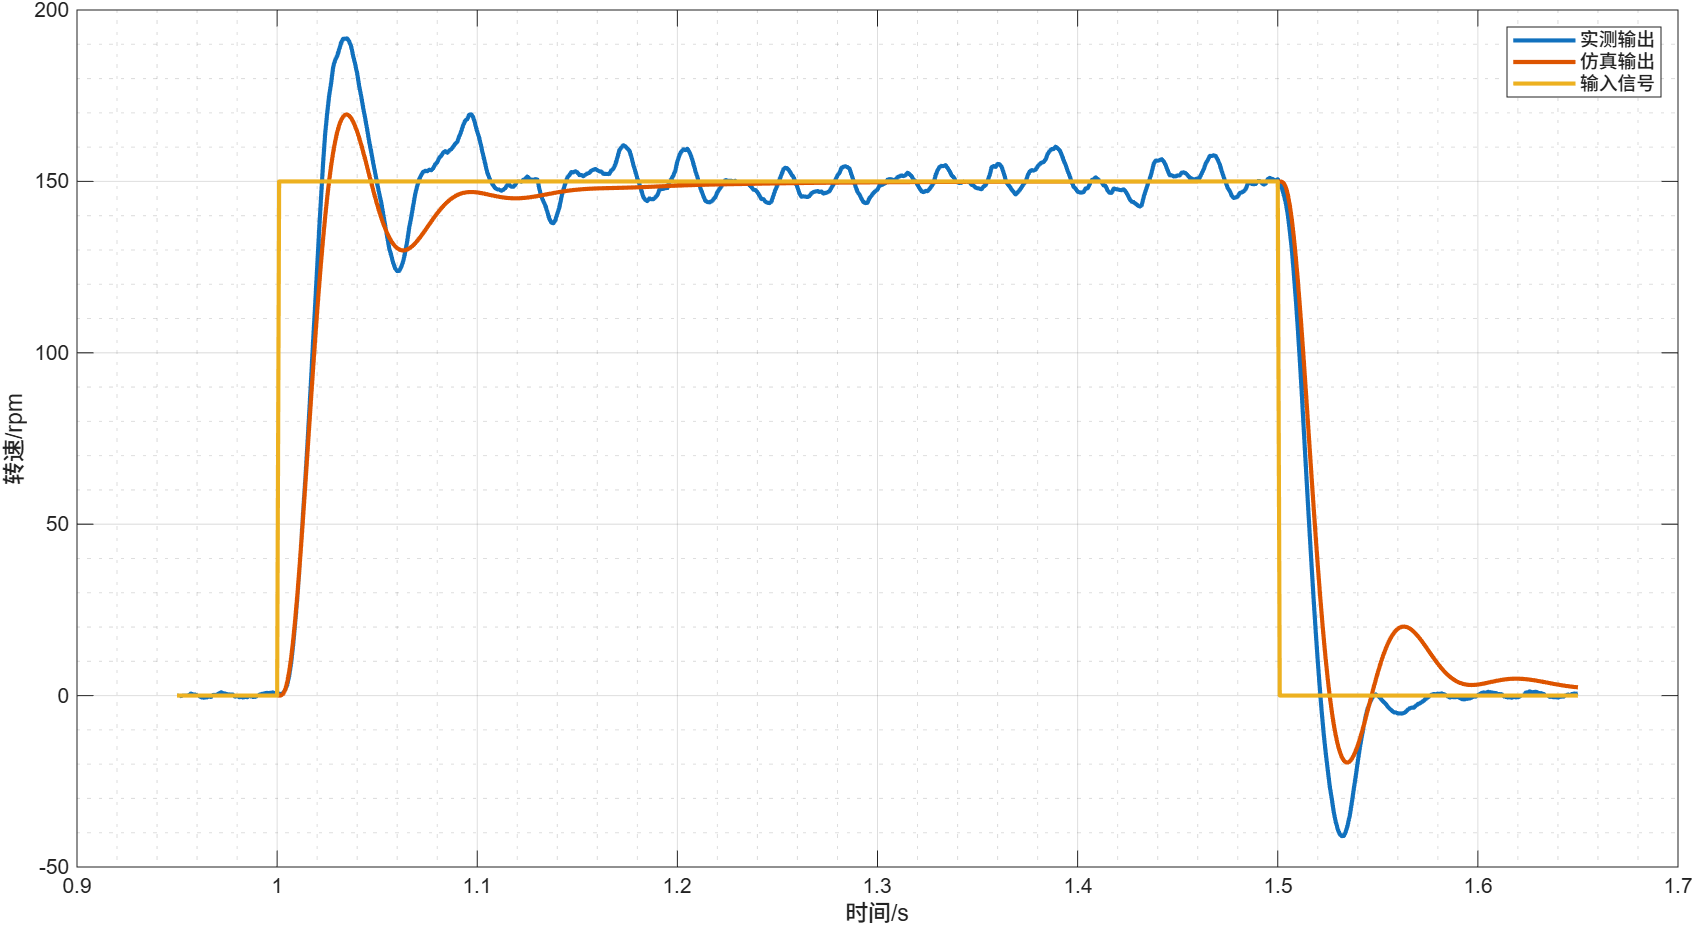
\includegraphics[width=\textwidth]
        {图片/速度环正向方波闭环验证.png}
        \caption{速度环正向方波闭环验证}
    \end{minipage}
    \begin{minipage}{0.5\textwidth}
        \centering
        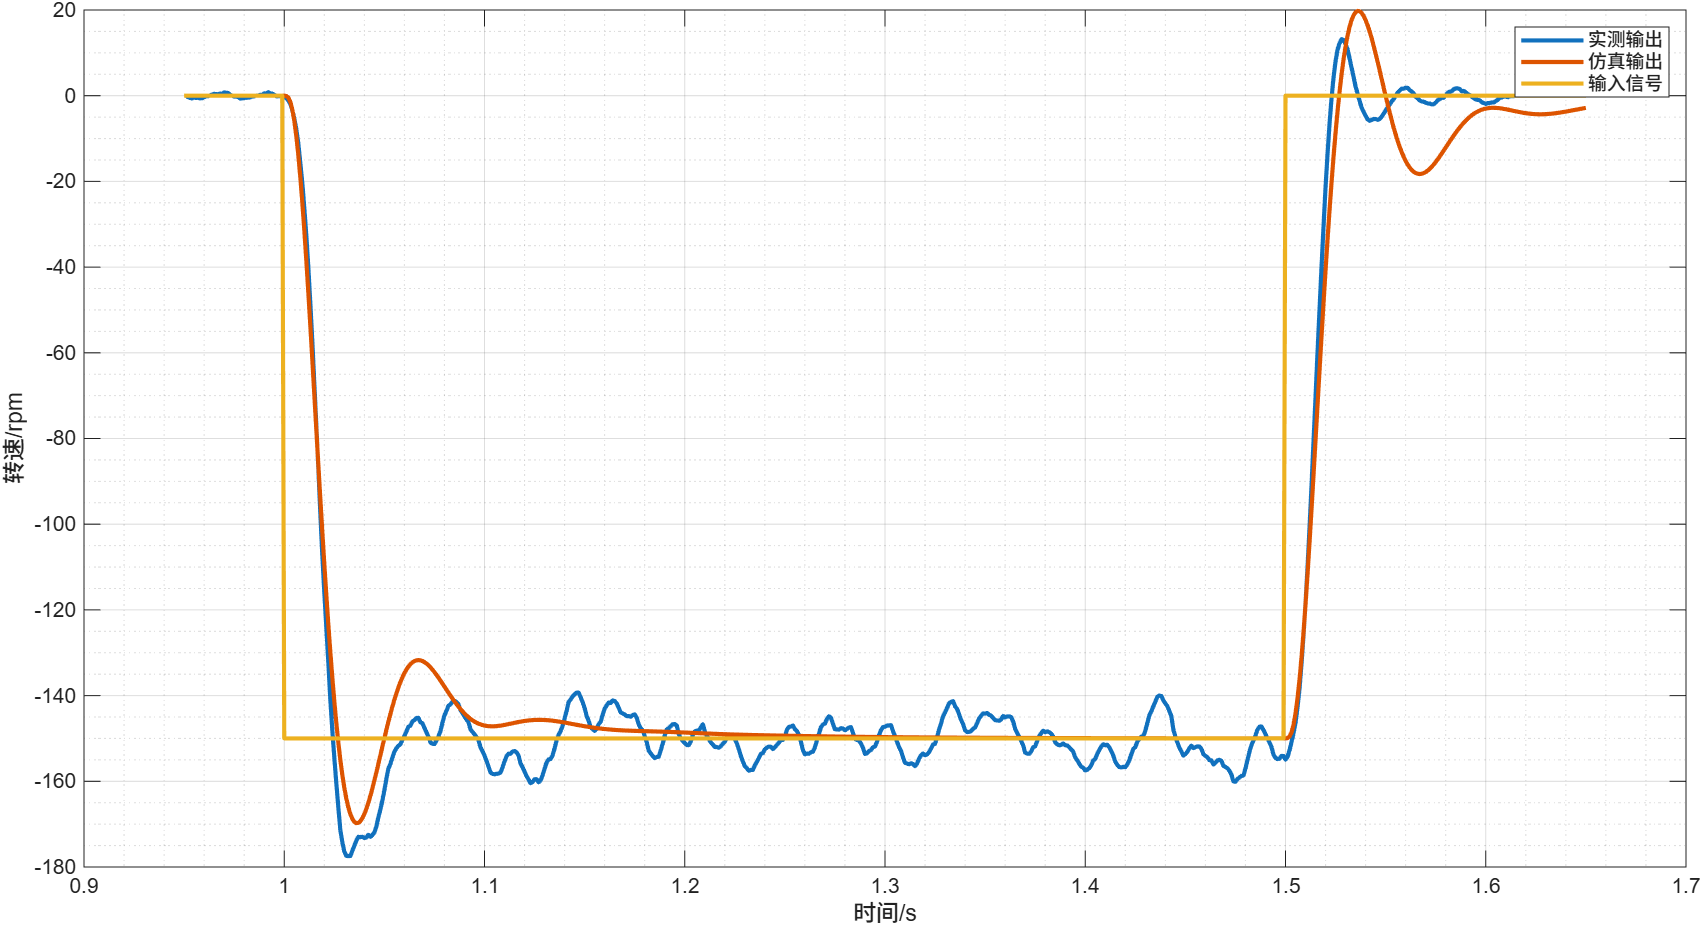
\includegraphics[width=\textwidth]
        {图片/速度环负向方波闭环验证.png}
        \caption{速度环负向方波闭环验证}   
    \end{minipage}
\end{figure}

与开环验证结果类似，仿真和实测波形在暂态段基本一致。进入稳态后惯性力矩趋于零，
齿槽转矩作为周期性扰动凸显出来，此时即使用闭环控制器也无法完全消除其带来的转速振荡，因此稳态段偏差较大。
正向方波相关系数99.34643\%，拟合优度86.99273\%；
负向方波相关系数99.05066\%，拟合优度85.20157\%，拟合水平低于电流闭环验证。
原因有三：其一，速度回路的非线性干扰强度和来源均高于电路部分，线性传递函数的拟合精度天然更低；
其二，速度环辨识在Q轴电流闭环下进行，闭环效应（积分饱和、输出限幅）使系统特性较开环时更为复杂，降低了验证结果的准确性；
其三，电路部分有明确的解析结构（一阶RL电路），可据此修正辨识偏差，而速度环被控对象即使采用
经典的\(\cfrac{1}{Js+B}\)模型，也在该电机上存在显著的不适配。
需要说明的是，闭环验证拟合优度低于开环验证并非表明辨识结果更不可信：如\ref{sec:反推结果的敏感性分析}所述，
开环验证的拟合优度主要受极低频段（直流稳态）误差拖累，而闭环验证中该误差被速度环积分环节压制，
剩余偏差主要源于核心频段模型误差与速度测量噪声的反馈放大，以及上述三点原因。因此闭环验证拟合优度
有所降低属预期现象，模型可信度仍由开环验证确立。整体上拟合优度均大于85\%，仍属可接受范围。

最后，在上述测试过程中对\(i_{\mathrm{d}}=0\)的理想化假设验证如下图所示。
正向方波闭环测试过程中，反电动势相关系数99.99993\%，拟合优度99.88057\%；电磁转矩相关系数100.00000\%，拟合优度99.97844\%；
负向方波闭环测试过程中，反电动势相关系数99.99992\%，拟合优度99.87166\%；电磁转矩相关系数100.00000\%，拟合优度99.98025\%。
\begin{figure}[H]
    \begin{minipage}{0.5\textwidth}
        \centering
        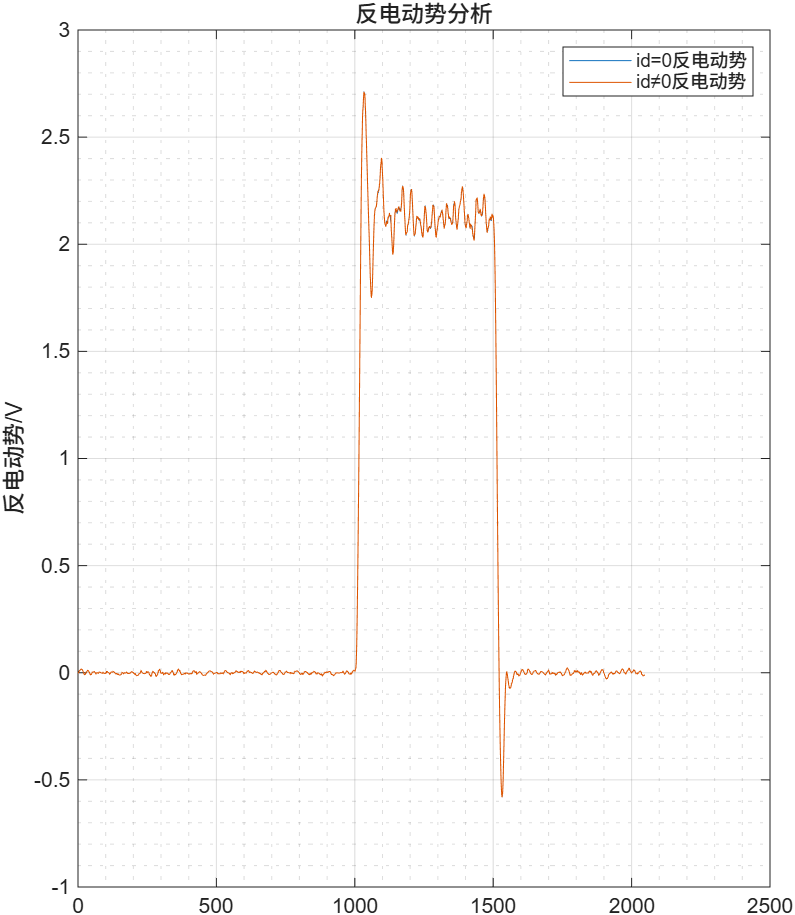
\includegraphics[width=\textwidth]
        {图片/速度环正向闭环方波反电动势对比.png}
        \caption{速度环正向闭环方波反电动势对比}
    \end{minipage}
    \begin{minipage}{0.5\textwidth}
        \centering
        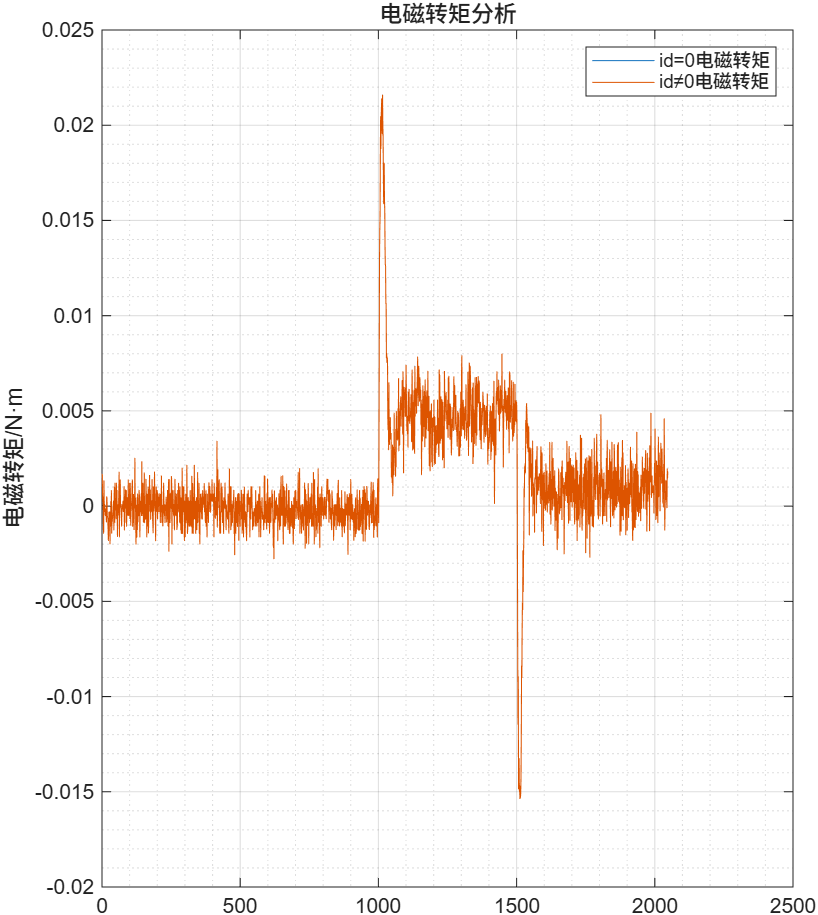
\includegraphics[width=\textwidth]
        {图片/速度环正向闭环方波电磁转矩对比.png}
        \caption{速度环正向闭环方波电磁转矩对比}
    \end{minipage}
\end{figure}
\begin{figure}[H]
    \begin{minipage}{0.5\textwidth}
        \centering
        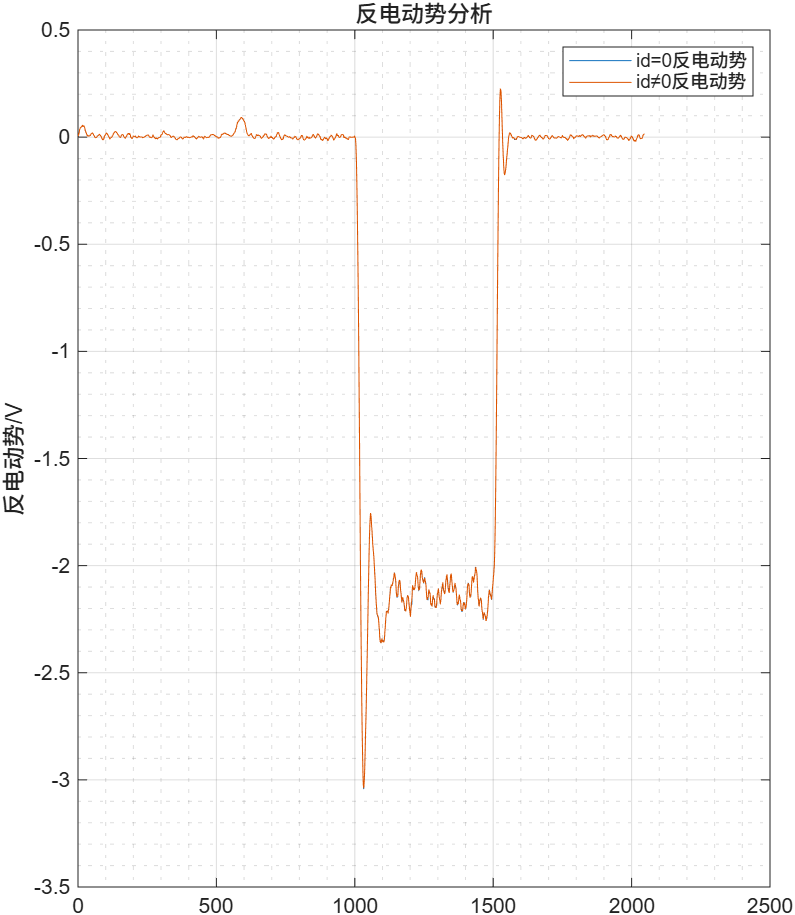
\includegraphics[width=\textwidth]
        {图片/速度环负向闭环方波反电动势对比.png}
        \caption{速度环负向闭环方波反电动势对比}
    \end{minipage}
    \begin{minipage}{0.5\textwidth}
        \centering
        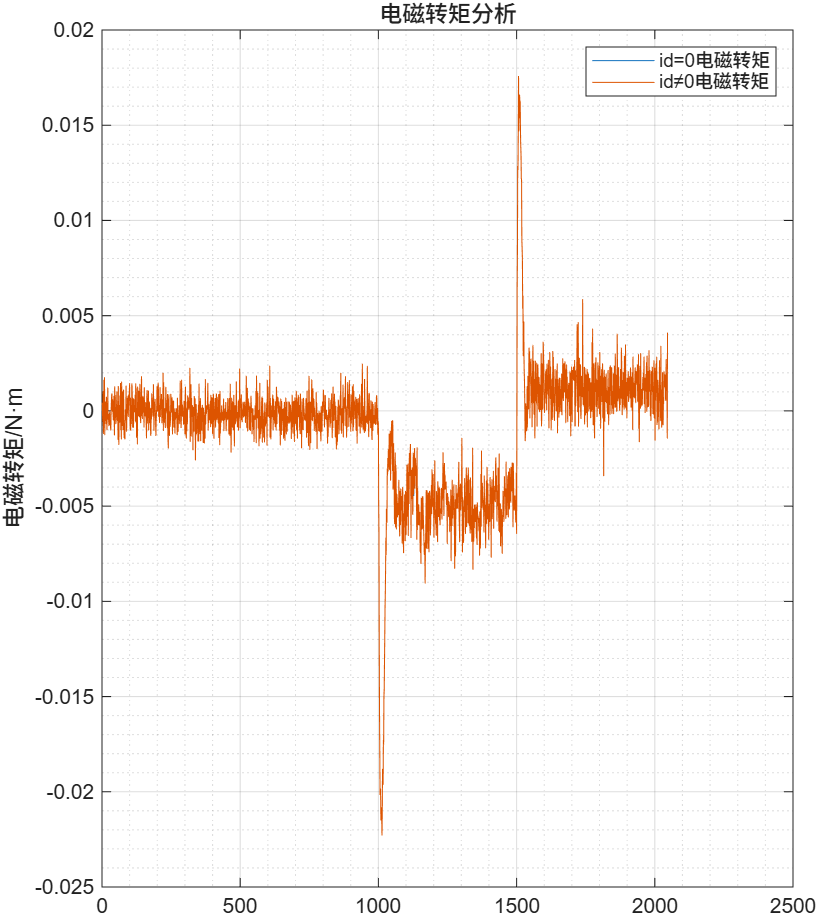
\includegraphics[width=\textwidth]
        {图片/速度环负向闭环方波电磁转矩对比.png}
        \caption{速度环负向闭环方波电磁转矩对比}
    \end{minipage}
\end{figure}

\subsubsection{反电动势前馈补偿分析}
上述测试证实了在\(i_{\mathrm{d}}=0\)控制下反电动势与电磁转矩的理想化假设均成立，且模型精度极高。
那么进行反电动势前馈补偿，以进一步改善速度环响应应当是可行的。
为此，在\(C_{\mathrm{Q}}(s)\)输出端叠加前馈项\(\hat{E}=\cfrac{\pi}{30}np\hat{\psi}_{\mathrm{m}}\)，加入前馈后的系统框图如下图所示。
\begin{figure}[H]
    \centering
    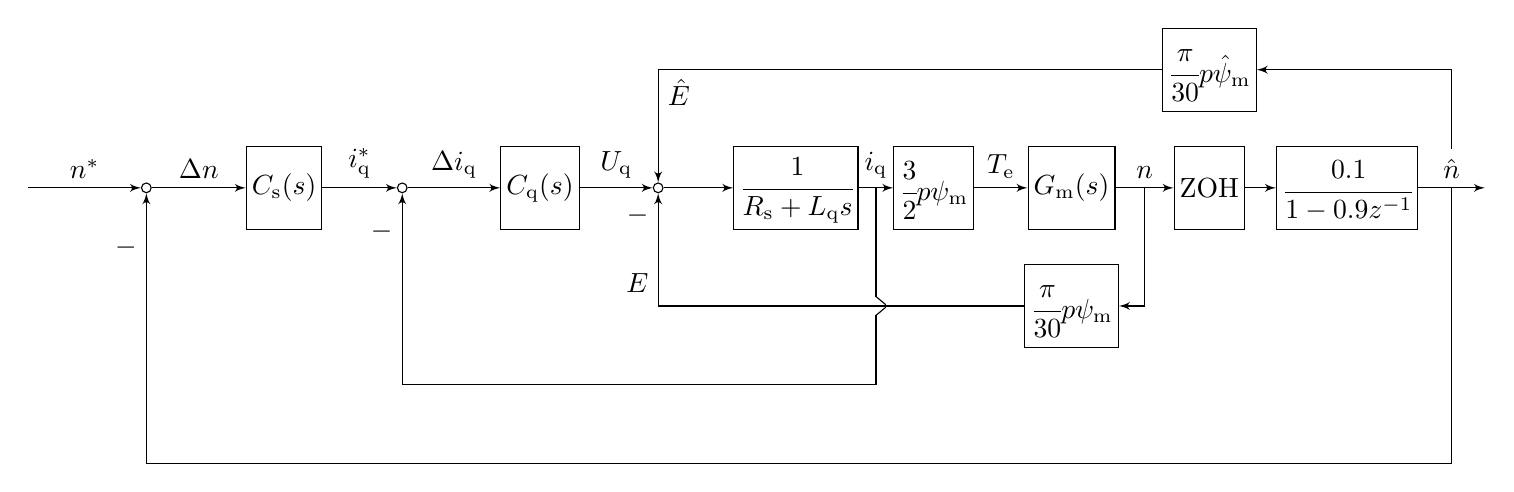
\begin{tikzpicture}[auto, node distance=1.75cm, >=latex']
        % 样式定义
        \tikzstyle{block} = [draw, rectangle, minimum height=3em, minimum width=1.8em, align=center, inner sep=2pt]
        \tikzstyle{sum} = [draw, circle, node distance=1.5cm, minimum size=0.35em, inner sep=0pt]
        \tikzstyle{input} = [coordinate]
        \tikzstyle{output} = [coordinate]
        \tikzstyle{feedback} = [coordinate]

        % 放置节点
        \node [input, name=input] {};
        \node [sum, right of=input] (sum1) {};
        \node [block, right of=sum1] (Cs) {\(C_{\mathrm{s}}(s)\)};
        \node [sum, right of=Cs] (sum2) {};
        \node [block, right of=sum2] (Cq) {\(C_{\mathrm{q}}(s)\)};
        \node [sum, right of=Cq] (sum) {};
        \node [block, right of=sum] (RL) {\(\cfrac{1}{R_{\mathrm{s}}+L_{\mathrm{q}} s}\)};
        \node [block, right of=RL] (K) {\(\cfrac{3}{2}p\psi_{\mathrm{m}}\)};
        \node [block, right of=K] (Mech) {\(G_{\mathrm{m}}(s)\)};
        \node [block, right of=Mech] (ZOH) {ZOH};
        \node [block, right of=ZOH] (Filter) {\(\cfrac{0.1}{1-0.9z^{-1}}\)};
        \node [output, right of=Filter] (output) {};
        \node [block, below of=Mech, node distance=1.5cm] (Kf) {\(\cfrac{\pi}{30}p\psi_{\mathrm{m}}\)};
        \node [feedback, below of=sum, node distance=3.5cm] (F) {};
        \node [feedback, below of=Cq,node distance=2.5cm] (Fb) {};
        \node [block, above of=ZOH, node distance=1.5cm] (FF) {\(\cfrac{\pi}{30}p\hat{\psi}_{\mathrm{m}}\)};

        \draw [->] (input) -- node {\(n^*\)} (sum1);
        \draw [->] (sum1) -- node {\(\Delta n\)} (Cs);
        \draw [->] (Cs) -- node {\(i_{\mathrm{q}}^*\)} (sum2);
        \draw [->] (sum2) -- node {\(\Delta i_{\mathrm{q}}\)} (Cq);
        \draw [->] (Cq) -- node {\(U_{\mathrm{q}}\)} (sum);
        \draw [->] (sum) -- node {} (RL);
        \draw [->] (RL) -- node [name=iq] {\(i_{\mathrm{q}}\)} (K);
        \draw [->] (K) -- node {\(T_{\mathrm{e}}\)} (Mech);
        \draw [->] (Mech) -- node [name=y] {\(n\)} (ZOH);
        \draw [->] (ZOH) -- node {} (Filter);
        \draw [->] (Filter) -- node [name=y_fi] {\(\hat{n}\)} (output);
        % 反电动势反馈
        \draw [->] (y) |- (Kf);
        \draw [->] (Kf) -| node[pos=0.9] {\(-\)} node [pos=0.6] {\(E\)} (sum);
        % i_{\mathrm{q}}反馈：在交叉点处加桥接小弧（跳线），与反电动势线路交叉但不连接
        \coordinate (cross) at (iq |- Kf);
        \coordinate (jT) at ([yshift=0.12cm] cross);
        \coordinate (jB) at ([yshift=-0.12cm] cross);
        \draw [-] (iq) -- (jT);
        \draw [-] (jT) -- ++(0.12, -0.1) -- ++(0, -0.04) -- ++(-0.12, -0.1);
        \draw [-] (jB) |- (Fb);
        \draw [->] (Fb) -| node[pos=0.9] {\(-\)} node [pos=0.6] {} (sum2);
        \draw [-] (y_fi) |- (F);
        \draw [->] (F) -| node[pos=0.9] {\(-\)} node [pos=0.6] {} (sum1);
        \draw [->] (y_fi) |- (FF);
        \draw [->] (FF) -| node[pos=0.6] {\(\hat{E}\)} (sum);
    \end{tikzpicture}
    \caption{Q轴双闭环控制系统框图（带反电动势前馈）}
    \label{fig:Q轴双闭环控制系统框图（带反电动势前馈）}
\end{figure}

采用原先的控制器，分别测试在前馈补偿前后的方波响应，结果如下图所示。
\begin{figure}[H]
    \centering
    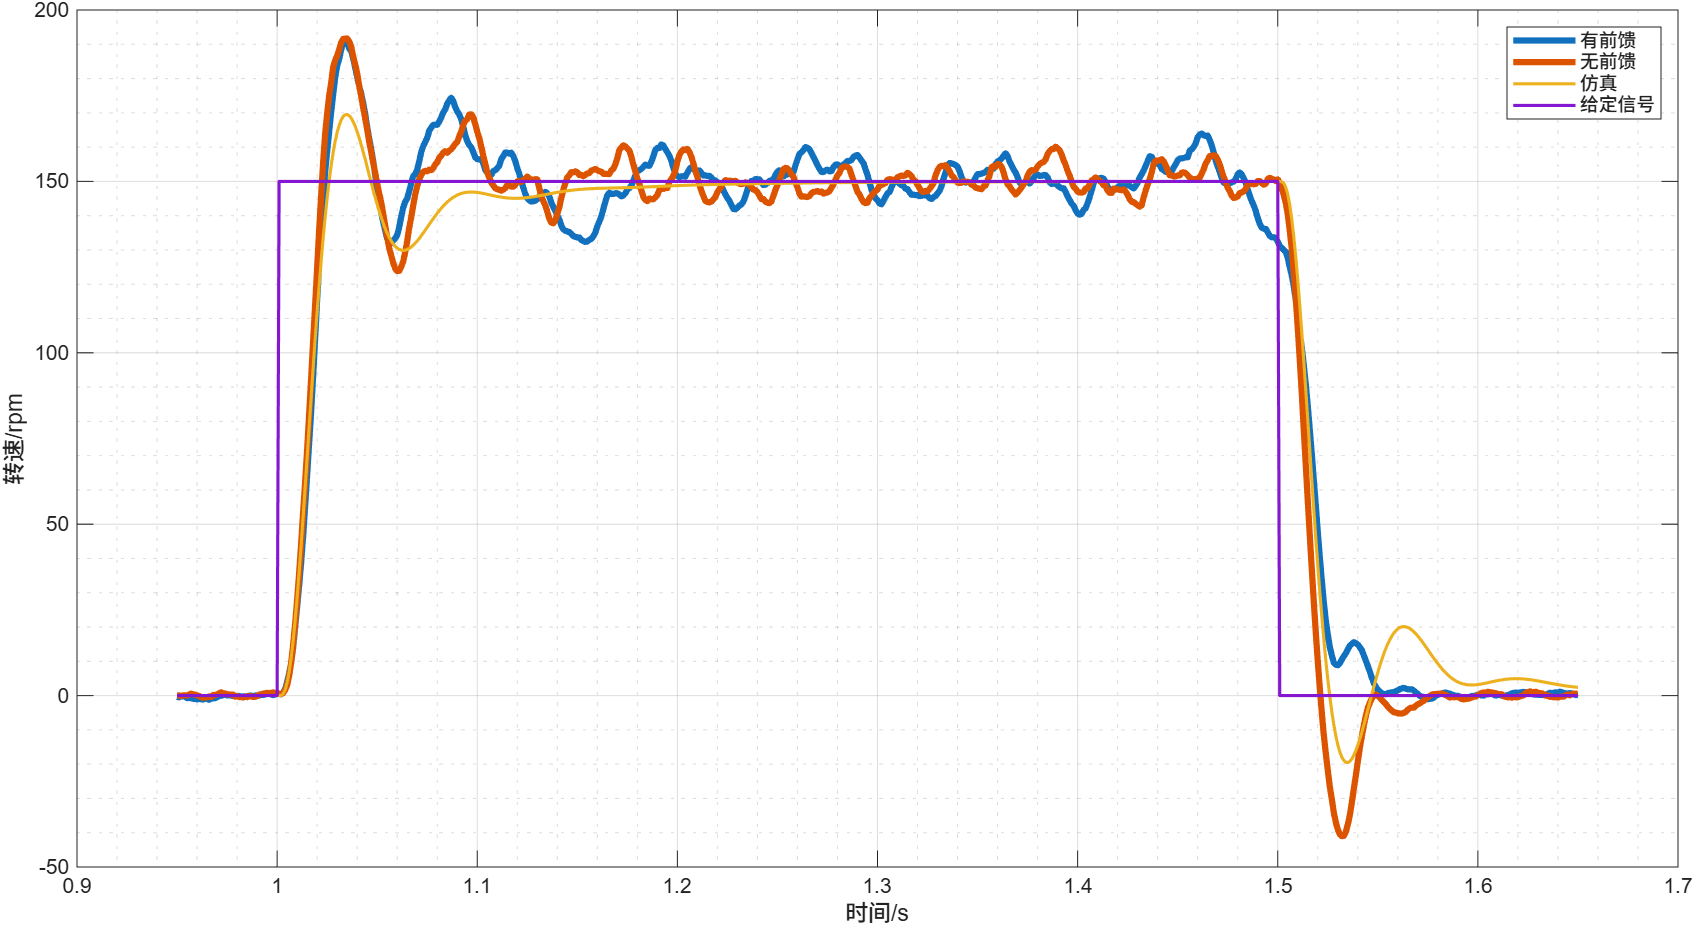
\includegraphics[width=\textwidth]
    {图片/前馈补偿对比.png}
    \caption{前馈补偿对比}
\end{figure}

可以发现，补偿前后响应有所改善，但没有达到质变的程度。
分析其原因在于反电动势在奇异摄动系统中的双重属性。对闭环带宽高达2kHz、控制采样频率15kHz的电流内环而言，反电动势
近似于缓慢变化的直流扰动（因为在设计时没有考虑），设计的控制器\(C_{\mathrm{Q}}(s)\)能够很好地压制其作用。而
对于闭环带宽仅21Hz、控制采样频率1kHz的速度外环而言，反电动势的变化正好落在其核心工作频段内。

上述双重属性带来了两个影响，其一是电流环控制器本身足以压制反电动势扰动，前馈补偿带来的收益有限；其二是对于速度环
被控对象设计而言反电动势的物理路径依然存在且不可忽略，求解速度环被控对象时仍然要在电流环和反电动势闭环耦合的情况下
进行。若直接忽视反电动势闭环简化被控对象求解，会过于乐观地轻视了被控对象的复杂特性，设计出的控制器基本不可用
\footnote{经测试，即使用很保守的参数设计控制器依然会导致系统发散}。

综上所述，本章采用的分步策略：电流环控制器设计、含反电动势的速度环建模、频域校正设计在电机控制器设计上是
更鲁棒的做法，而反电动势的前馈补偿在这其中并不是必要步骤。

%附录
\appendix
\ctexset{
    section={
        name={},
        number={附录\Alph{section}}
    }
}
\setcounter{tocdepth}{1}
\addtocontents{toc}{\protect\setcounter{tocdepth}{1}}

\newpage
\section{线性代数与离散系统分析基础知识}
\subsection{线性代数知识补充}
首先介绍\textbf{凯莱-哈密顿定理（Cayley-Hamilton Theorem）}。对于一个\(n\)阶的方阵\(\bm{A}\)，其特征方程可以表示为：
\begin{equation*}
    \det(\bm{A}-\lambda \bm{I}) = 0 = a_{0}+a_{1}\lambda+a_{2}\lambda^2+\cdots+a_{n}\lambda^n=f(\lambda)
\end{equation*}

这是一条代数方程。而凯莱-哈密顿定理指出，方阵\(\bm{A}\)同样会满足特征方程：
\begin{equation*}
    a_{0}+a_{1}\bm{A}+\bm{A}^2+\cdots+a_{n}\bm{A}^n=f(\bm{A})=0
\end{equation*}

对上式进行变换，可以得到：
\begin{equation*}
    \bm{A}^n = -\cfrac{1}{a_{n}}(a_{0}+a_{1}\bm{A}+a_{2}\bm{A}^2+\cdots+a_{n-1}\bm{A}^{n-1})
\end{equation*}

也就是说，\(\bm{A}^n\)可以表示为\(\bm{A}^0\sim \bm{A}^{n-1}\)的线性组合结果。若对上式同时左乘\(\bm{A})\)，则可以得到：
\begin{equation*}
    \bm{A}^{n+1} = \bm{A}^n+1 = -\cfrac{1}{a_{n}}(a_{0}+a_{1}\bm{A}+a_{2}\bm{A}^2+\cdots+a_{n-1}\bm{A}^{n})
\end{equation*}

可知\(\bm{A}^{n+1}\)可以表示为\(\bm{A}^\sim \bm{A}^{n}\)的线性组合结果。由于\(\bm{A}^n\)可以表示为\(\bm{A}^0\sim \bm{A}^{n-1}\)的线性组合，
因此\(\bm{A}^{n+1}\)也可以表示为\(\bm{A}^0\sim \bm{A}^{n-1}\)的线性组合。根据数学归纳法可知：

\textbf{对\(n\)阶方阵\(\bm{A}\)，\(\forall k\ge n\)，\(\bm{A}^k\)可以表示为\(\bm{A}^0\sim \bm{A}^{n-1}\)的线性组合。}

其次介绍矩阵的\textbf{奇异值分解（Singular Value Decomposition,SVD）}，这是后续系统辨识最核心的知识。

对于\(n\)阶方阵\(\bm{A}\)，可以求取其秩为\(\textrm{rank} (\bm{A})\)，秩的值表示了\(\bm{A}\)矩阵具有多少个非零的特征值。
但对于非方阵\(\bm{A})\)必然是不满秩不能进行特征值分解的，但可以进行奇异值分解。因此奇异值分解可以视为特征值分解在任意维矩阵上的推广。

根据方阵的特征值分解公式，方阵\(\bm{A}\)可以表示为：
\begin{equation*}
    \bm{A} = \bm{P}\bm{\Lambda}\bm{P}^{-1}
\end{equation*}

其中\(\bm{P}\)为特征向量矩阵，\(\bm{\Lambda}\)为特征值组成的对角矩阵。奇异值分解说明任意矩阵\(\bm{A}\)都可以表示为：
\begin{equation}
    \bm{A} = \bm{U}\bm{\Sigma}\bm{V}^T
    \label{eq:奇异值分解}
\end{equation}

其中\(\bm{U}\)为左奇异矩阵，\(\bm{\Sigma}\)为奇异值组成的对角矩阵，\(\bm{V}\)为右奇异矩阵。需要注意的是，奇异值是非负的，
因为他表示矩阵在各个维度上的能量分布。

最后介绍\textbf{托普利茨矩阵（Toeplitz Matrix）}，这在求解离散卷积方程中非常有用。托普利茨矩阵定义为
\textbf{从左上到右下，每一个对称对角线上具有完全相同元素的矩阵}。比如一个四阶托普利茨矩阵为
\(
\bm{\mathcal{T}} = 
\begin{bmatrix}
    4 & 1 & 0 & 2 \\
    3 & 4 & 1 & 0 \\
    2 & 3 & 4 & 1 \\
    1 & 2 & 3 & 4 \\
\end{bmatrix}
\)。

特殊地，如果一个托普利茨矩阵从左下到右上，每一个对称对角线上也具有相同的元素，则称为对称托普利茨矩阵。比如
一个四阶的对称托普利茨矩阵为
\(
\bm{\mathcal{T}} = 
\begin{bmatrix}
    4 & 3 & 2 & 1 \\
    3 & 4 & 3 & 2 \\
    2 & 3 & 4 & 3 \\
    1 & 2 & 3 & 4 \\
\end{bmatrix}
\)。

\subsection{离散系统知识补充}
离散系统的状态空间方程与连续系统类似，可以表示为：
\begin{equation}
    \begin{cases}
        x_{k+1} = \bm{A} x_{k} + \bm{B} u_{k} \\
        y_{k} = \bm{C} x_{k} + \bm{D} u_{k}
    \end{cases}
    \label{eq:离散状态空间方程}
\end{equation}

利用状态空间方程\ref{eq:离散状态空间方程}，可以得到系统的传递函数：
\begin{equation}
    G(z)=\bm{C}(zI-\bm{A})^{-1}\bm{B}+\bm{D}
    \label{eq:离散传递函数}
\end{equation}

其中\(z\)为\(\mathcal{Z}\)变换的变量，与拉普拉斯变换的\(s\)变量对应，两者满足\(z=e^{Ts}\)，其中\(T\)表示离散系统的采样时间。

一个系统的传递函数，就是其脉冲响应的拉普拉斯变换。同理，在离散系统中，其传递函数是脉冲响应序列的\(\mathcal{Z}\)变换。
假设系统的脉冲响应序列为\(g_{k}\)），则其传递函数可以表示为：

\begin{equation*}
    G(z)=\sum_{k=0}^{\infty}g_{k}z^{-k}
\end{equation*}

而根据\ref{eq:离散传递函数}，可以使用类似于下式的无穷级数展开：
\begin{equation*}
    \cfrac{1}{1-x}=1+\sum_{k=1}^{\infty}x^k
\end{equation*}

对于\((z\bm{I}-\bm{A})^{-1}\)，可以表示为\(z^{-1}(\bm{I}-z^{-1}\bm{A})^{-1}\)。后者可以无穷级数展开得到：
\begin{equation*}
    (\bm{I}-z^{-1}\bm{A})^{-1} =\bm{I}+z^{-1}\bm{A}+z^{-2}\bm{A}^2+\cdots=\sum_{k=0}^{\infty}z^{-k}\bm{A}^k
\end{equation*}

带入传递函数可得：
\begin{equation*}
    G(z)=\bm{C}(z\bm{I}-\bm{A})^{-1}\bm{B}+\bm{D}=
    \bm{C}z^{-1}\sum_{k=0}^{\infty}z^{-k}\bm{A}^k\bm{B}+\bm{D}=
    \bm{D}+\sum_{k=0}^{\infty}\bm{C}\bm{A}^k\bm{B}z^{-(k+1)}=\sum_{k=0}^{\infty}g_{k}z^{-k}
\end{equation*}

因此脉冲响应序列满足：
\begin{equation}
    g_{k} = 
    \begin{cases}
        \bm{D} & k=0 \\
        \bm{C}\bm{A}^{k-1}\bm{B} & k\ge 1
    \end{cases}
    \label{eq:脉冲响应序列}
\end{equation}

这也称为离散系统的\textbf{马尔科夫系数（Markov Coefficient）}。而根据凯莱-哈密顿定理，对于\(n\)阶方阵\(\bm{A}\)（同时\(n\)也是系统阶次），
\(\forall k\ge n\)，\(\bm{A}^k\)可以表示为\(\bm{A}^0\sim \bm{A}^{n-1}\)的线性组合。因此可以得到离散系统一个重要的性质，即
\textbf{\(n\)阶离散系统的脉冲响应序列只有前\(n\)个值是独立的，后续的值都可以被前\(n\)个值线性表示}。

为了将这一个性质直观表示，进行进一步分析，可以构造离散系统的\textbf{汉克尔矩阵（Hankel Matrix）}。离散系统的汉克尔矩阵定义为：
\begin{equation}
    \bm{\mathcal{H}} =
    \begin{bmatrix}
        g_{1} & g_{2} & \cdots & g_{n} \\
        g_{2} & g_{3} & \cdots & g_{n+1} \\
        \vdots & \vdots & \ddots & \vdots \\
        g_{n} & g_{n+1} & \cdots & g_{2n-1}
    \end{bmatrix}
    \label{eq:汉克尔矩阵}
\end{equation}

根据离散系统的特性，可知\(n\)阶离散系统的汉克尔矩阵是满秩的。如果对汉克尔矩阵进行奇异值分解，也应该得到\(n\)个非零的奇异值。


\newpage
\section{Ho-Kalman辨识算法\label{sec:Ho-Kalman辨识过程介绍}}
\subsection{激励信号的选取}
理论上来说，Ho-Kalman算法对于输入信号没有要求。但是输入信号需要激励出被控系统的主要模态，这要求输入信号频谱尽可能宽，在系统的
主要模态附近的激励能力要远远超出采样噪声。

一种常见的输入激励信号为\textbf{伪随机二进制序列（Pseudo-Random Binary Sequence，PRBS）}中的最大长度序列，记为\textbf{M序列}。
在时域上，M序列表现为以幅值\(\pm A\)不断变换的、间隔为\(T_s\)的、周期为\(2^{N}-1\)的序列。这里点明了M序列的三个核心参数：
幅值\(A\)、采样周期\(T_s\)、级数\(N\)。

M序列的特点是近似为白噪声，自相关尖锐，便于进行相关分析辨识。当然也有坏处。根据功率谱分析可知，M序列在直流分量（0Hz）附近
基本没有激励能力，即采样M序列对于系统的开环放大系数辨识效果很差。因此一般会使用阶跃信号产生直流分量，确定开环放大系数和工作点；然后
在等到系统阶跃响应基本结束后叠加M序列，进行工作点附近的系统辨识。

M序列的三个参数需要慎重选取，这决定着辨识结果：

\begin{itemize}
    \item 幅值\(A\)：一般而言，幅值越高，激励能力越强，信噪比越高。但过高的幅值可能会导致系统偏离工作点附近的线性区间，反而降低
    辨识结果。
    \item 采样周期\(T_s\)：采样周期越高，采样频率越高，辨识结果越好。但采样频率越高，数据采集和上传难度越高。一般选择采样周期
    \(\cfrac{1}{T_s}\ge 10f_c\)，其中\(f_c\)为预估的系统截止频率。
    \item 级数\(N\)：级数越高，伪随机在频域上的频点间隔越小，但相应的每个频点上的激励能力下降。而级数N也影响着辨识时长。对于大部分
    机电系统，推荐选取N=9\(\sim\)12。
\end{itemize}

M序列的产生一般采用反馈移位寄存器实现，代码实现较为简单，只是需要占据很长的一段空间存储。如下是一个给定级数N=11的M序列实现函数，此时周期为\(2^{N}-1=2047\)。输出结果存储在数组m\(\_\)seq[2047]中，用0和1表示结果。

\begin{lstlisting}
void generate_m_sequence_11(unsigned char m_seq[])
{
        uint16_t lfsr = 0x7FF;        // 11位寄存器初始状态（全1）
        const uint16_t mask = 0x7FF;  // 低11位掩码

        for (int i = 0; i < 2047; i++) {
            // 当前输出为寄存器最高位（bit10）
            m_seq[i] = (lfsr >> 10) & 1u;

            // 反馈：bit10 异或 bit1（对应本原多项式 x^11 + x^2 + 1）
            uint16_t feedback = ((lfsr >> 10) ^ (lfsr >> 1)) & 1u;

            // 移位并插入反馈，保持11位有效
            lfsr = ((lfsr << 1) | feedback) & mask;
        }
}
\end{lstlisting}
\subsection{系统脉冲响应的求解}

通过输入伪随机信号，得到了输入序列\(x_k\)和输出序列\(y_k\)，长度为\(M=2^N-1\)。
第一步是计算脉冲响应序列。若离散系统的脉冲响应序列为\(g_k\)，则会满足：
\begin{equation}
    y_k=x_k * g_k
    \label{eq:离散时域卷积方程}
\end{equation}

但是由于采样噪声存在，直接求解上述的离散卷积方程结果往往会很差，因此需要稍作变换（具体原理见
\ref{sec:噪声作用下的相关分析法简介}）。此处需要的不是采样噪声，而是其中的有效信息，
因此可以求解输入信号的\textbf{自相关序列（Self-Correlation Sequence）}：
\footnote{若有时域信号\(x\)和\(y\)，相关运算指的是进行\(R_{xy}(\tau)=\text{E}[x(t)y(t+\tau)]\)，
即在不同的偏移情况下求解两个信号对应元素相乘的期望。若两个信号完全一致（与自身做相关运算）则称为自相关，若不一致则称为互相关。
相关函数特点是，在一定偏移下两个信号的统计学相关性越高，相关函数在此处的值相较于其他地方会更高。若两个信号在没有统计学相关性则相关函数为
\(R_{xy}(\tau)=\text{E}[x(t)]\cdot \text{E}[y(t+\tau)]\)为两者均值之积。
}
\begin{equation*}
    R_{xx}(k)=\cfrac 1M\sum_{i=0}^{M-1} x_{i} x_{i+k} =\cfrac 1M(x_{-k} * x_{k})
\end{equation*}

输入与输出信号的\textbf{互相关序列（Cross-Correlation Sequence）}：
\begin{equation*}
    R_{xy}(k)=\cfrac 1M\sum_{i=0}^{M-1} x_{i} y_{i+k} =\cfrac 1M(x_{-k} * y_{k})
\end{equation*}

其中\(x_{-k}\)表示输入序列\(x_{k}\)的时间反转。
\footnote{相关运算和卷积是类似的，卷积是“信号反转后滑动平均”的过程，而相关运算将一个输入信号反转后卷积，相当于
“信号不反转直接滑动平均”的过程。}
而对于时域卷积方程\ref{eq:离散时域卷积方程}，两边同时与\(x_{-k}\)卷积并乘上序列长度倒数
\(\cfrac 1M\)可得：
\begin{equation*}
    \cfrac 1M x_{-k}*y_k=\cfrac 1Mx_{-k}*x_k*g_k
\end{equation*}

也就可以表示为：
\begin{equation}
    R_{xy}(k)=R_{xx}(k)*g_k
    \label{eq:维纳-霍普夫方程}
\end{equation}

该方程称为\textbf{维纳-霍普夫方程（Wiener-Hopf Equation）}，是相关分析法的核心所在。
该方程表明，通过相关序列变换，可以视为输入了时域自相关序列，输出信号为时域互相关序列。

在得到了输入自相关序列和互相关序列后，接下来需要求解系统的脉冲响应序列，也就是求解维纳-霍普夫方程\ref{eq:维纳-霍普夫方程}。该方程
可以展开为：
\begin{equation*}
    R_{xy}(k)=\sum_{j=0}^{N-1}R_{xx}(k-j)\times g_j
\end{equation*}

可以将其改写为矩阵形式：
\begin{equation*}
    \begin{bmatrix}
        R_{xy}(0)\\
        R_{xy}(1)\\
        \vdots\\
        R_{xy}(N-1)
    \end{bmatrix}
    =
    \begin{bmatrix}
        R_{xx}(0)&R_{xx}(1)&R_{xx}(2)&\cdots&R_{xx}(N-1)\\
        R_{xx}(1)&R_{xx}(0)&R_{xx}(1)&\cdots&R_{xx}(N-2)\\
        R_{xx}(2)&R_{xx}(1)&R_{xx}(0)&\cdots&R_{xx}(N-3)\\
        \vdots&\vdots&\vdots&\ddots&\vdots\\
        R_{xx}(N-1)&R_{xx}(N-2)&R_{xx}(N-3)&\cdots&R_{xx}(0)
    \end{bmatrix}
    \begin{bmatrix}
        g_0\\
        g_1\\
        \vdots\\
        g_{N-1}
       \end{bmatrix}
\end{equation*}

定义向量
\(\textbf{r}_{xy}=\begin{bmatrix}
        R_{xy}(0)\\
        R_{xy}(1)\\
        \vdots\\
        R_{xy}(N-1)
    \end{bmatrix}\)
和\(\textbf{g}=\begin{bmatrix}
        g_0\\
        g_1\\
        \vdots\\
        g_{N-1}
    \end{bmatrix}\)

可以发现矩阵
\(\textbf{r}_{xx}=
    \begin{bmatrix}
        R_{xx}(0)&R_{xx}(1)&R_{xx}(2)&\cdots&R_{xx}(N-1)\\
        R_{xx}(1)&R_{xx}(0)&R_{xx}(1)&\cdots&R_{xx}(N-2)\\
        R_{xx}(2)&R_{xx}(1)&R_{xx}(0)&\cdots&R_{xx}(N-3)\\
        \vdots&\vdots&\vdots&\ddots&\vdots\\
        R_{xx}(N-1)&R_{xx}(N-2)&R_{xx}(N-3)&\cdots&R_{xx}(0)
    \end{bmatrix}
    \)
从左上到右下，每一个对称对角线上的元素均相等（如第一个为\(R_{xx}(0)\)，第二个为\(R_{xx}(1)\)，第三个为\(R_{xx}(2)\)），为
托普利茨矩阵。

通过构造自相关的托普利茨矩阵，可以将离散的卷积方程，改写为矩阵乘法方程：

\begin{equation*}
    \textbf{r}_{xy}=\textbf{r}_{xx}\textbf{g}
\end{equation*}

脉冲响应序列可以通过矩阵求逆计算得到：

\begin{equation}
    \textbf{g}=\textbf{r}_{xx}^{-1}\textbf{r}_{xy}
    \label{eq:脉冲响应序列求解}
\end{equation}

如下图是针对三轴云台方位轴速度环辨识过程中得到的输入相关序列、输入输出自相关序列和脉冲响应序列：

\begin{figure}[H]
    \begin{minipage}{0.5\textwidth}
        \centering
        
\includegraphics[width=0.8\textwidth]
        {图片/输入自相关序列.jpg}
        \caption{输入自相关序列}
        \label{fig:输入自相关序列}
    \end{minipage}
    \begin{minipage}{0.5\textwidth}
        \centering
        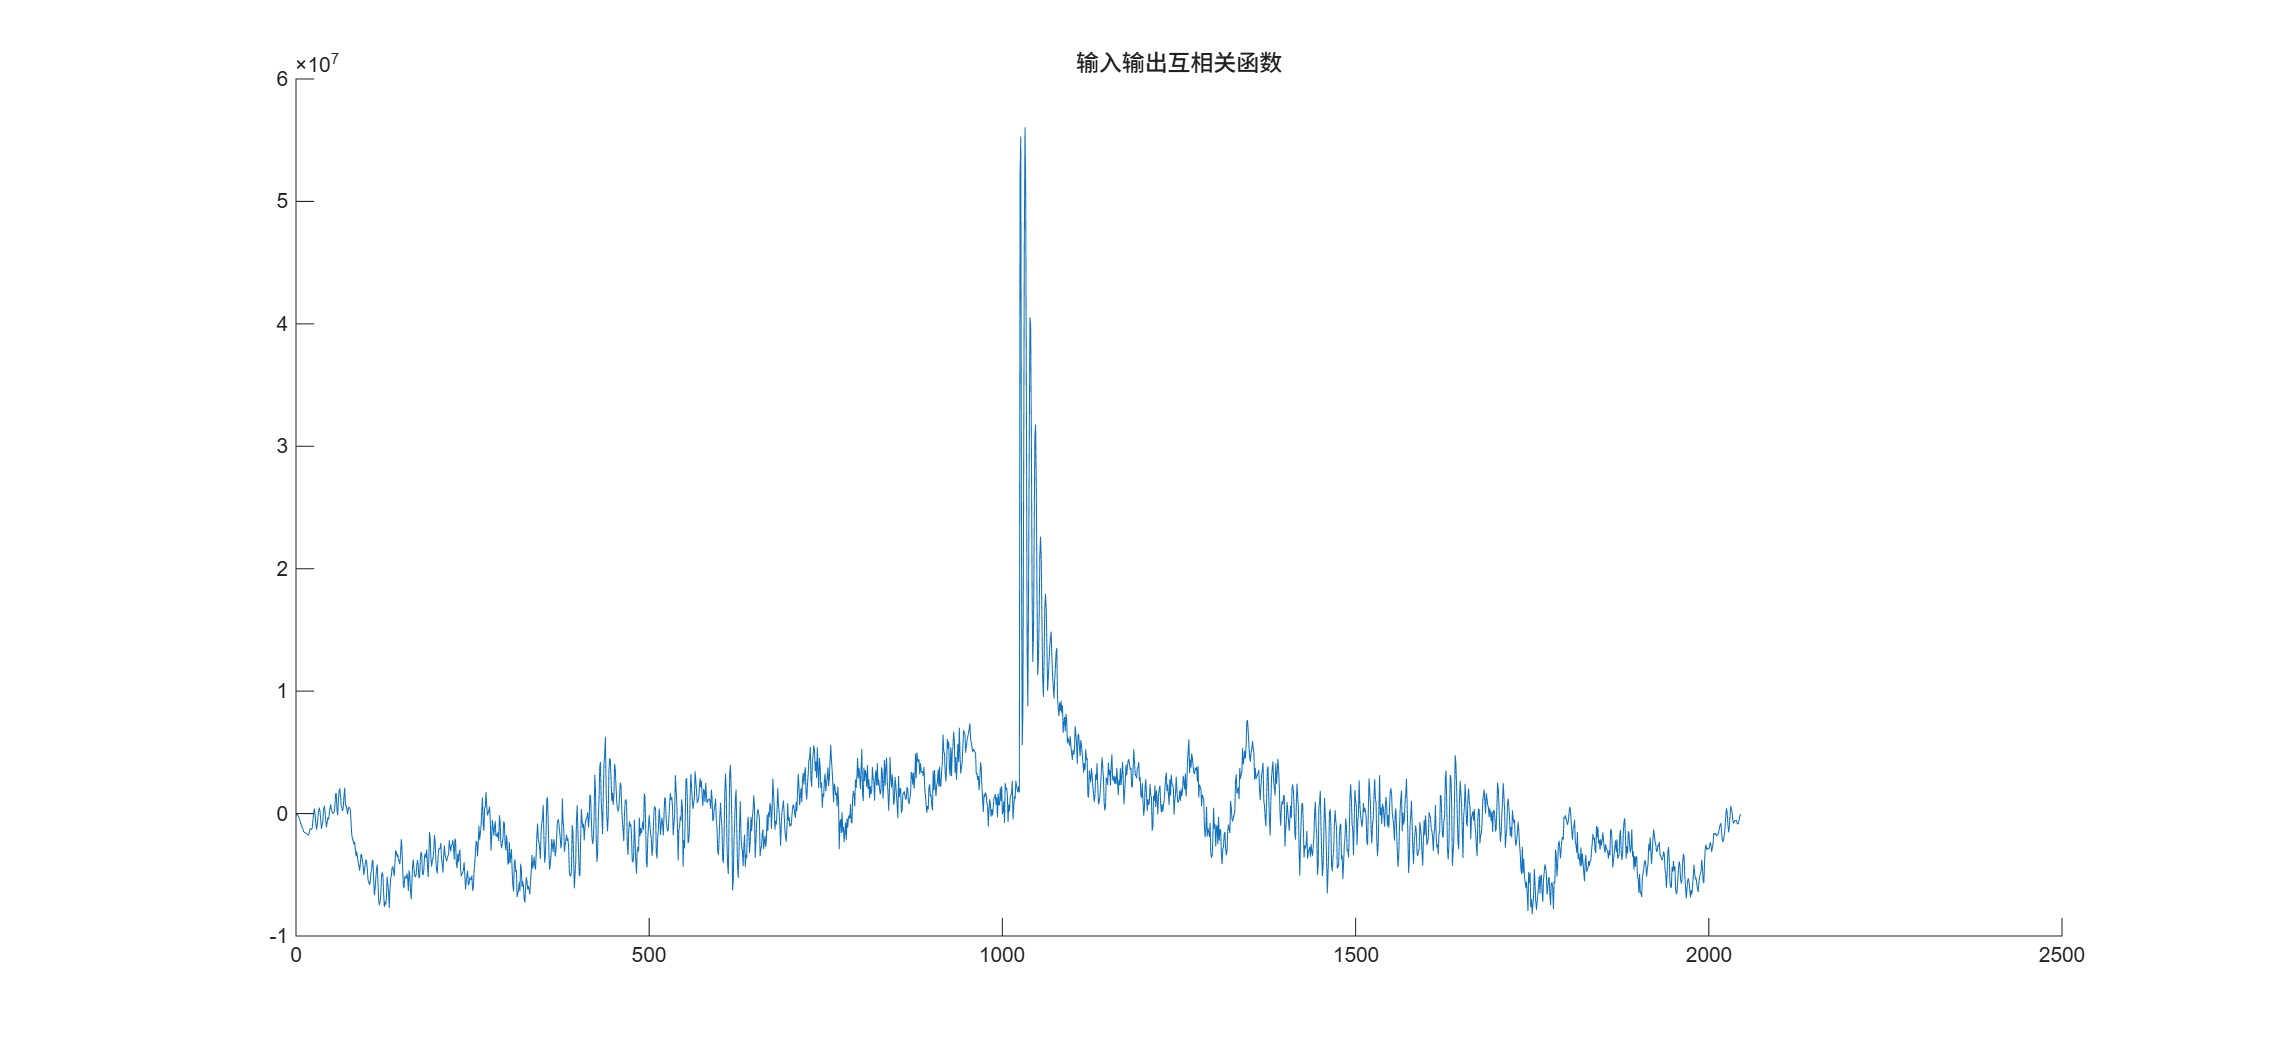
\includegraphics[width=0.8\textwidth]
        {图片/输入输出互相关序列.jpg}
        \caption{输入输出互相关序列}
        \label{fig:输入输出互相关序列}
    \end{minipage}
\end{figure}

\begin{figure}[H]
    \centering
    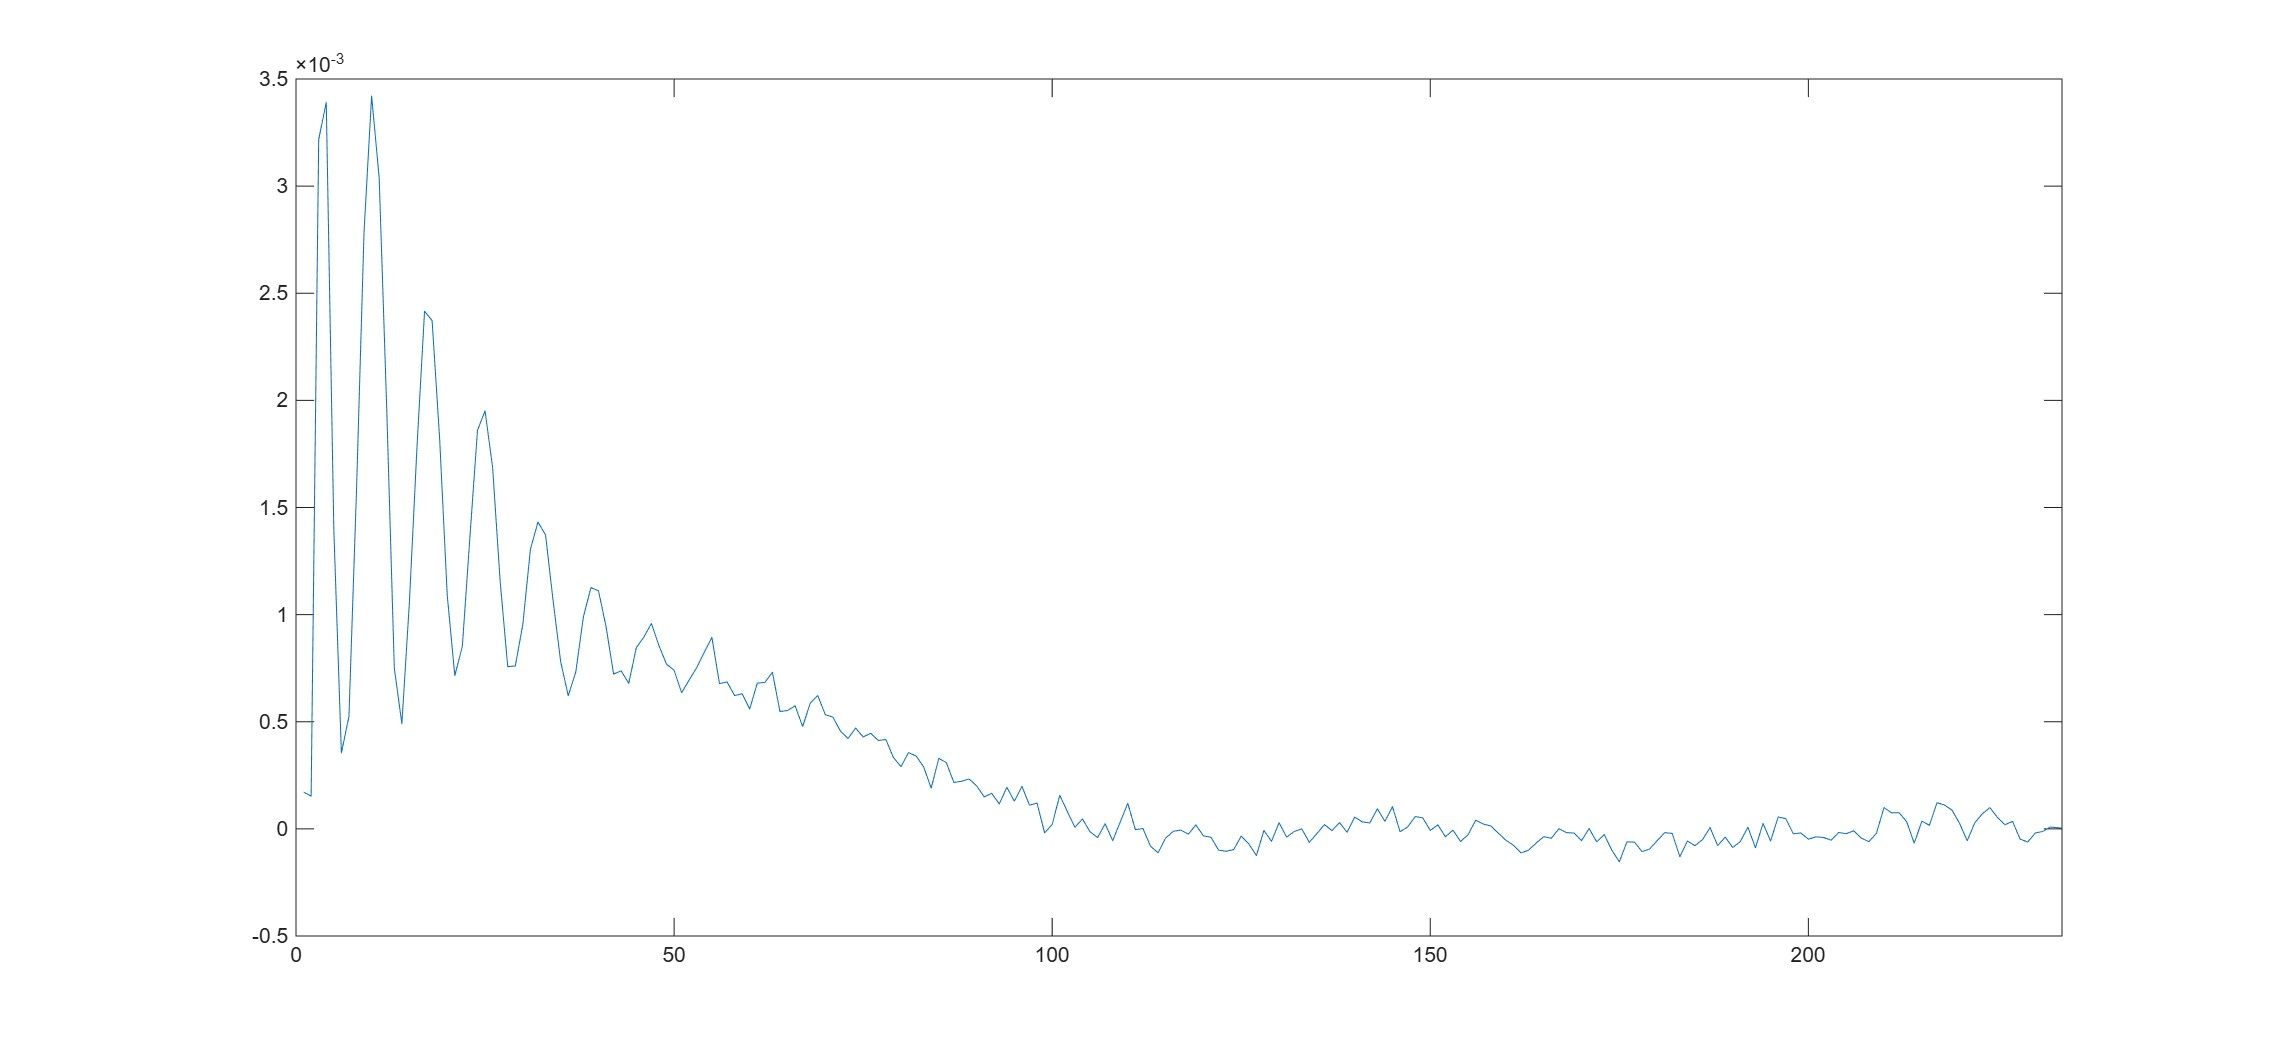
\includegraphics[width=0.8\textwidth]
    {图片/脉冲响应序列.jpg}
    \caption{脉冲响应序列（截取部分）}
    \label{fig:脉冲响应序列}
\end{figure}

\subsection{系统阶次的确定}

得到脉冲响应序列后，可以按照\ref{eq:汉克尔矩阵}的定义构造系统的汉克尔矩阵。根据离散系统分析的相关知识，若系统本身是n阶的，
那么汉克尔矩阵奇异值分解后会有n个主导奇异值。若系统本身是m阶的，那么理想情况下只要构造的汉克尔矩阵阶次n>m即可包含全部的模态。
但是由于采样噪声存在，便是得到的脉冲响应序列并不理想，因此如何选取汉克尔矩阵的阶次
会极大的影响后续的辨识结果。

以永磁同步电机的辨识为例，其求解得到的脉冲响应序列如\ref{fig:脉冲响应序列}所示。可以发现，即使经过了相关运算降噪，
在系统响应结束后仍会有噪声产生的波动，此时系统本身信息接近零，信噪比极低，因此最好的方法是\textbf{选取暂态响应过程构成汉克尔矩阵}。
而构造一个n阶的汉克尔矩阵，需要用到\(g_1\)到\(g_{2n-1}\)的信息。据图求出暂态响应基本结束的时刻（\ref{fig:脉冲响应序列}为20），将其
除以2，即所构造的汉克尔矩阵阶次。在这里选取构造8阶的汉克尔矩阵。

确定汉克尔矩阵阶次后，按照\ref{eq:奇异值分解}进行奇异值分解。在系统阶次判断时，无需关心奇异值的绝对值，只关心奇异值的相对关系，
关心有几个主导（非零）奇异值，因此对齐进行归一化，得到归一化奇异值分解如下图所示。

\begin{figure}[H]
    \centering
    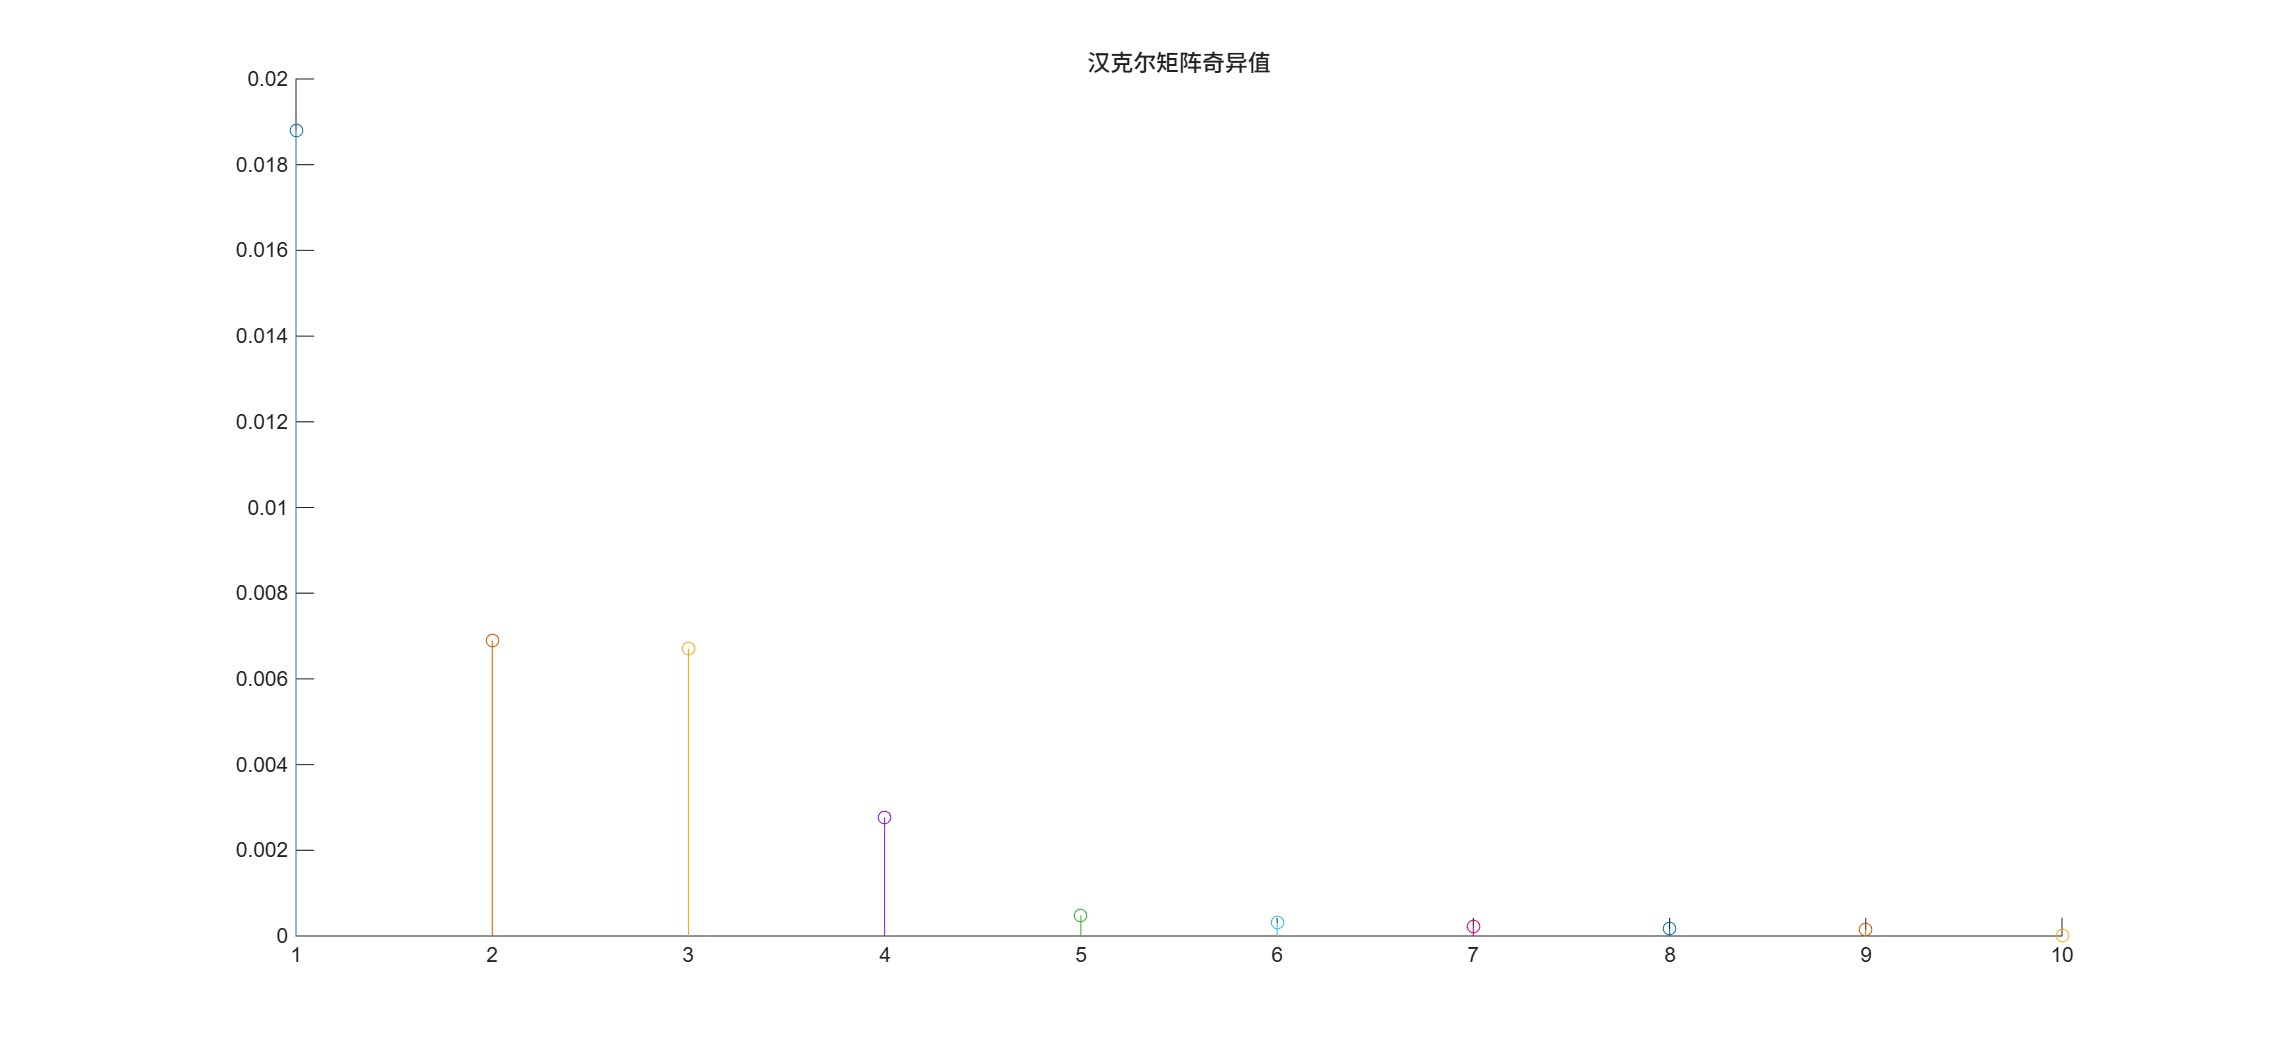
\includegraphics[width=0.8\textwidth]
    {图片/归一化奇异值分解图.jpg}
    \caption{归一化奇异值分解图}
    \label{fig:归一化奇异值分解}
\end{figure}

据图可知，前四个奇异值非零，后续的奇异值基本归零，因此可以判断系统为四阶系统。

\subsection{最小空间实现与传递函数计算}

至此已经得到了系统的汉克尔矩阵\(\mathcal{H}\)，
并完成了奇异值分解得到\(\mathcal{H}=U\Sigma V^T\)，也知道了系统的阶次。如何求解
最小状态空间实现需要的A，B，C，D是接下来讨论的内容。

汉克尔矩阵的定义式为：

\begin{equation*}
    \mathcal{H}=
    \begin{bmatrix}
        g_1 & g_2 & \cdots & g_{n} \\
        g_2 & g_3 & \cdots & g_{n+1} \\
        \vdots & \vdots & \ddots & \vdots \\
        g_{n} & g_{n+1} & \cdots & g_{2n-1}
    \end{bmatrix}
\end{equation*}

根据马尔科夫系数\ref{eq:脉冲响应序列}，可以将汉克尔矩阵改写为：

\begin{equation*}
    \mathcal{H}
    =
    \begin{bmatrix}
        CB & CAB & \cdots & CA^{n-1}B \\
        CAB & CA^2B & \cdots & CA^nB \\
        \vdots & \vdots & \ddots & \vdots \\
        CA^{n-1}B & CA^nB & \cdots & CA^{2n-2}B
    \end{bmatrix}
    =
    \begin{bmatrix}
        C\\CA\\CA^2\\\vdots\\CA^{n-1}
    \end{bmatrix}
    \begin{bmatrix}
        B&AB&A^2B&\cdots&A^{n-1}B
    \end{bmatrix}
     =\mathcal{O}\mathcal{C}
\end{equation*}

也即汉克尔矩阵是能控性矩阵\(\mathcal{C}\)与能观性矩阵\(\mathcal{O}\)之积，
结合汉克尔矩阵的奇异值分解\(\mathcal{H}=U\Sigma V^T\)，系统辨识可以认为：

\begin{equation*}
    \begin{cases}
        \mathcal{O}&=U\Sigma^{0.5} \\
        \mathcal{C}&=\Sigma^{0.5}V^T
    \end{cases}
\end{equation*}

其中\(\Sigma^{0.5}\)表示对奇异值逐个元素取平方根。

求取得到能控性矩阵和能观性矩阵后，根据其定义和确定的系统阶次k，可以得到
\textbf{输入矩阵B由能控性矩阵\(\mathcal{C}\)的第一列前k个元素构成，
输出矩阵为C由能观性矩阵\(\mathcal{O}\)第一行的前k个元素构成}。

为了计算A，可以构造移位汉克尔矩阵：

\begin{equation*}
    \mathcal{H'}=
    \begin{bmatrix}
        g_2 & g_3 & \cdots & g_{n+1} \\
        g_3 & g_4 & \cdots & g_{n+2} \\
        \vdots & \vdots & \ddots & \vdots \\
        g_{n+1} & g_{n+2} & \cdots & g_{2n}
    \end{bmatrix}
\end{equation*}

同样用马尔科夫系数带入得到：

\begin{equation*}
    \mathcal{H'}
    =
    \begin{bmatrix}
        CAB & CA^2B & \cdots & CA^{n}B \\
        CA^2B & CA^3B & \cdots & CA^{n+1}B \\
        \vdots & \vdots & \ddots & \vdots \\
        CA^{n}B & CA^{n+1}B & \cdots & CA^{2n-1}B
    \end{bmatrix}
    =
    \begin{bmatrix}
        C\\CA\\CA^2\\\vdots\\CA^{n-1}
    \end{bmatrix}
    A
    \begin{bmatrix}
        B&AB&A^2B&\cdots&A^{n-1}B
    \end{bmatrix}
    =\mathcal{O}A\mathcal{C}
\end{equation*}

因此A'可以计算为：

\begin{equation*}
    A'=\mathcal{O}^{-1}\mathcal{H'}\mathcal{C}^{-1}
\end{equation*}

而进行截断后，k阶系统实际的\textbf{状态矩阵A由A'的前k行k列的元素构成}。

馈通矩阵D一般由两种做法，第一种是直接忽略视为0，因为实际系统基本不存在随输入信号立刻改变的分量。第二种是辨识认为
\(D=g_0\)。一般为了让辨识结果更符合实际，会选择第二种做法。

得到了四个矩阵后，可以计算得到传递函数\(G(z)=C(zI-A)^{-1}B+D\)，至此，基于Ho-Kalman算法的系统辨识就完成了。

\newpage
\section{基于相关分析的Ho-Kalman辨识有偏-无偏性分析}
\label{sec:基于相关分析的Ho-Kalman辨识有偏-无偏性分析}
\subsection{噪声作用下的相关分析法简介\label{sec:噪声作用下的相关分析法简介}}
在\ref{sec:Ho-Kalman辨识过程介绍}中介绍了电机参数辨识所用到的Ho-Kalman辨识算法，其大致包含以下几个步骤：
\begin{itemize}
    \item 求取输入的自相关序列与输入输出的互相关序列，利用维纳-霍普夫方程求取系统的脉冲响应序列
    \item 利用系统的脉冲响应序列（离散系统的马尔科夫系数）构造系统的汉克尔矩阵
    \item 对汉克尔矩阵进行奇异值分解确定系统阶次
    \item 利用汉克尔矩阵和系统的阶次，估计系统的状态空间实现
    \item 根据估计得到状态空间实现，求取系统的传递函数
\end{itemize}

Ho-Kalman算法由B.L.Ho（何炳麟）和R.E.Kalman（鲁道夫·E·卡尔曼）在《Regelungstechnik》\footnote{德语，意为《控制技术》}上
发表的《Effective construction of linear state-variable models from input/output functions》
（1966）中提出
\footnote{1965年以《Effective construction of linear state-variable models from input/output data》为题，
在第3届Allerton电路与系统理论会议以会议论文形式预印，正文中提到是正式发表的版本}，
当时他们分析的是如何从确定已知的脉冲响应序列中估计系统的阶次，并构造最小子空间实现和求取传递函数，而如何获取系统的脉冲响应序列
严格意义上并不属于Ho-Kalman算法的内容。工程上使用维纳-霍普夫方程求解脉冲响应序列则是相关分析法的内容，是早期与Ho-Kalman算法搭配实现
系统辨识的工具。

Ho-Kalman辨识算法提出了如何从已知的脉冲响应序列中构造系统的状态空间实现，奠定了现代子空间辨识算法的核心思想。但从系统辨识性质来看，
上述基于维纳-霍普夫方程相关分析求解脉冲响应序列的
Ho-Kalman辨识算法属于\textbf{开环辨识算法}，即默认待辨识的系统不处于闭环中。若将其运用于闭环环节的辨识，辨识结果将是有偏的，
而有偏来源并不在Ho-Kalman算法本身，而主要来自维纳-霍普夫方程的相关分析过程。

根据线性时不变系统的卷积性质，输入序列\(x_k\)、输出序列\(y_k\)与系统脉冲响应序列\(g_k\)满足：
\begin{equation*}
    y_k = g_k * x_k
\end{equation*}

假设\(x_k\)为无噪声的理想输入，输出端存在采样噪声\(n_{y,k}\)，则实测输出为：
\begin{equation*}
    y_k = g_k * x_k + n_{y,k}
\end{equation*}

用矩阵表示为：
\begin{equation*}
    \textbf{Y}=\textbf{X}\textbf{g}+\textbf{n}_y
\end{equation*}

若直接在时域上进行最小二乘估计\footnote{这正是矩阵方程求解脉冲响应序列的本质，在时域进行最小二乘拟合。}，
脉冲响应序列的估计值为：
\begin{equation*}
    \hat{\textbf{g}} = (\textbf{X}^T\textbf{X})^{-1}\textbf{X}^T\textbf{Y}
    = (\textbf{X}^T\textbf{X})^{-1}\textbf{X}^T(\textbf{X}\textbf{g}+\textbf{n}_y)
    = \textbf{g} + (\textbf{X}^T\textbf{X})^{-1}\textbf{X}^T\textbf{n}_y
\end{equation*}

为使估计一致（当数据长度\(N\to\infty\)时\(\hat{\textbf{g}}\to\textbf{g}\)），误差项需渐近为零：
\begin{equation*}
    \lim\limits_{N\to\infty}\frac{1}{N}\textbf{X}^T\textbf{n}_y = \mathbf{0}
\end{equation*}

上述式中\(\textbf{X}\)是由输入信号构成的托普利茨矩阵，那么\(\cfrac{1}{N}\textbf{X}^T\textbf{n}_y\)的每个元素
是输入与噪声的互相关运算结果。因此，使用相关运算将时域离散卷积转换为相关序列的卷积为：
\begin{equation*}
    R_{xy}[k]=g_k * R_{xx}[k]+R_{xn_y}[k]
\end{equation*}

矩阵表示为：
\begin{equation*}
    \textbf{r}_{xy}=\textbf{r}_{xx}\textbf{g}+\textbf{r}_{xn_y}
\end{equation*}

相关域下的脉冲响应估计为：
\begin{equation*}
    \hat{\textbf{g}}  = \textbf{r}_{xx}^{-1}\textbf{r}_{xy}
    = \textbf{g} + \textbf{r}_{xx}^{-1}\textbf{r}_{xn_y}
    \footnote{要求\(\textbf{r}_{xx}\)（由输入自相关序列排成的托普利茨矩阵）可逆。}
\end{equation*}

可以发现，无论是在时域上离散卷积还是在相关域上离散卷积，估计脉冲响应序列渐进一致都要求
\textbf{输入信号与输出测量噪声不相关}，这也是使用维纳-霍普夫方程估计脉冲响应序列并进行Ho-Kalman辨识可行的核心前提。
在开环条件下，输入与噪声来自独立源，该条件自然满足。
在闭环条件下，噪声经反馈回路进入输入通道，该条件一般不再成立。

值得一提的是，引入基于维纳-霍普夫方程的相关分析而非直接在时域求解卷积方程，主要是为了显式地提出无偏估计脉冲响应序列的
条件，即让输入信号和测量输出信号的噪声不相关\(R_{xn_y}[k]=0\)，这也是后续分析在闭环情况下估计脉冲响应序列有偏的出发点。

由于后续分析中所有信号均为离散采样序列，频域分析将采用\textbf{离散时间傅里叶变换（DTFT）}代替连续域的拉普拉斯变换。
对于自相关序列\(R_{xx}[k]\)，其DTFT即为\textbf{功率谱密度}：
\begin{equation*}
    S_{xx}(e^{j\omega})=\sum_{k=-\infty}^{\infty}R_{xx}[k]\,e^{-j\omega k}
\end{equation*}
互相关序列\(R_{xy}[k]\)的DTFT\(S_{xy}(e^{j\omega})\)同理定义。
由DTFT的卷积定理，离散卷积对应于频域乘积：若\(y_k = g_k * x_k\)，则\(Y(e^{j\omega})=G(e^{j\omega})X(e^{j\omega})\)，
其中\(G(e^{j\omega})\)为脉冲响应序列\(g_k\)的DTFT，即系统的\textbf{离散频率响应}。
\footnote{附录B中Ho-Kalman辨识得到的脉冲传递函数记为\(G(z)\)，
其在单位圆上的取值\(G(e^{j\omega})=\left.G(z)\right|_{z=e^{j\omega}}\)即为离散频率响应，以下统一以\(G(e^{j\omega})\)表示。}

\subsection{闭环的有偏-无偏性分析}
假设需要对下述系统利用维纳-霍普夫方程进行相关分析以求取脉冲响应序列：
\begin{center}
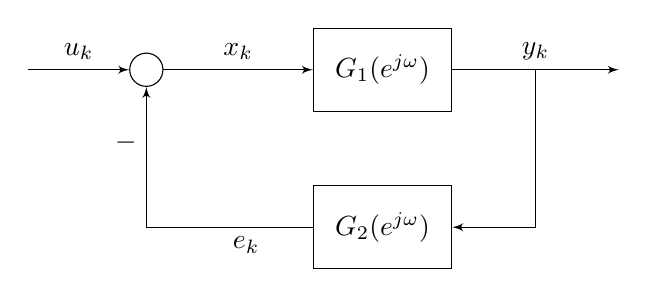
\begin{tikzpicture}[auto, node distance=3cm, >=latex']
    % 样式定义
    \tikzstyle{block} = [draw, rectangle, minimum height=3em, minimum width=5em, align=center]
    \tikzstyle{sum} = [draw, circle, node distance=1.5cm, minimum size=1.2em, inner sep=0pt]
    \tikzstyle{input} = [coordinate]
    \tikzstyle{output} = [coordinate]

    % 放置节点
    \node [input, name=input] {};
    \node [sum, right of=input] (sum) {};
    \node [block, right of=sum] (G1) {\(G_1(e^{j\omega})\)};
    \node [output, right of=G1] (output) {};
    \node [block, below of=G1, node distance=2cm] (G2) {\(G_2(e^{j\omega})\)};

    \draw [->] (input) -- node {\(u_k\)} (sum);
    \draw [->] (sum) -- node {\(x_k\)} (G1);
    \draw [->] (G1) -- node [name=y] {\(y_k\)} (output);
    \draw [->] (y) |- (G2);
    \draw [->] (G2) -| node[pos=0.2] {\(e_k\)} node[pos=0.8] {$-$} (sum);
\end{tikzpicture}
\end{center}

该系统的反馈回路来源于物理结构（如电机的反电动势），而不是人为造成的，也无法被人为解开。
因此在模型内部流转的信号均为无噪声的理想信号：
\begin{equation*}
    \begin{cases}
    x_{0,k}=u_k-e_{0,k}\\
    y_{0,k}=x_{0,k}*g_{1,k}\\
    e_{0,k}=y_{0,k}*g_{2,k}
    \end{cases}
\end{equation*}

而所有的噪声都在测量环节被引入，即实测用于分析的信号满足：
\begin{equation*}
    \begin{cases}
        x_k=x_{0,k}+n_{x,k}\\
        y_k=y_{0,k}+n_{y,k}\\
        e_k=e_{0,k}+n_{e,k}\\
    \end{cases}
\end{equation*}

认为上述噪声\(n_{x,k}\)、\(n_{y,k}\)、\(n_{e,k}\)是独立同分布的白噪声，且与理想信号无关。
假设可操作的变量为\(u_k\)，那么认为\(u_k\)是确定无噪声的信号。在上述前提下，进行基于维纳-霍普夫方程的脉冲响应求解，分析结论的
偏差性。

\subsubsection{中间到中间/输出}
选取\(x_k\)作为输入，而\(y_k\)作为输出，辨识前向通道频率响应\(G_1(e^{j\omega})\)。时域方程满足：
\begin{align*}
    y_k&=y_{0,k}+n_{y,k}\\
    &=g_{1,k}*x_{0,k}+n_{y,k}\\
    &=g_{1,k}*[x_k-n_{x,k}]+n_{y,k}\\
    &=g_{1,k}*x_k-g_{1,k}*n_{x,k}+n_{y,k}
\end{align*}

两侧同时对输入信号\(x_k\)进行相关运算得到：
\begin{align*}
    R_{xy}[k] = g_{1,k}*R_{xx}[k]+R_{x\omega}[k]
\end{align*}

其中\(\omega_k = -g_{1,k}*n_{x,k}+n_{y,k}\)表示等价输出噪声。根据\ref{sec:噪声作用下的相关分析法简介}中的分析可知，能够
无偏估计脉冲响应的充要条件是输入信号与输出噪声无相关，即\(R_{x\omega}[k]=0\)。将表达式代入相关运算的定义可得：
\begin{align*}
    R_{x\omega}[k] &= \text{E}[x_k\,\omega_{k+m}]\\
    &= \text{E}[x_k\times(-g_{1,k}*n_{x,k+m}+n_{y,k+m})]\\
    &= \text{E}[(x_{0,k}+n_{x,k})\times(-g_{1,k}*n_{x,k+m}+n_{y,k+m})]\\
    &= \text{E}[x_{0,k}\times(-g_{1,k}*n_{x,k+m})]+\text{E}[x_{0,k}\times n_{y,k+m}]
    + \text{E}[n_{x,k}\times(-g_{1,k}*n_{x,k+m})]+\text{E}[n_{x,k}\times n_{y,k+m}]
\end{align*}

不难发现，上述四个式子中，\(\text{E}[x_{0,k}\times(-g_{1,k}*n_{x,k+m})]=\text{E}[x_{0,k}\times n_{y,k+m}]=
\text{E}[n_{x,k}\times n_{y,k+m}]=0\)，因为\(x_{0,k}\)、\(n_{x,k}\)、\(n_{y,k}\)互不相关。但是\(\text{E}[n_{x,k}\times(-g_{1,k}*n_{x,k+m})]
\neq 0\)，因为\(n_{x,k}\)与自身是自相关的。使用维纳-霍普夫方程估计从\(x_k\)到\(y_k\)的脉冲响应是有偏的。

接下来具体量化这种偏差。根据上述分析可知\(R_{x\omega}[k]=\text{E}[n_{x,k}\times(-g_{1,k}*n_{x,k+m})]\)。根据
相关计算与卷积的关系可得：
\begin{align*}
    R_{x\omega}[k]&=-(n_{x,-k}*(g_{1,k}*n_{x,k}))[k]\\
    &=-g_{1,k} * (n_{x,-k}*n_{x,k})[k]\\
    &=-g_{1,k}*R_{n_xn_x}[k]
\end{align*}

上式中\(n_{x,-k}\)表示时序反转（与附录B中\(x_{-k}\)的约定一致）。对上式求取DTFT可得：
\begin{equation*}
    S_{x\omega}(e^{j\omega})=-G_1(e^{j\omega})S_{n_xn_x}(e^{j\omega})
\end{equation*}

对于理想噪声\(n_{x,k}\)而言，假设其服从正态分布\(n_{x,k}\sim N(0,\sigma_x^2)\)，则
\(R_{n_xn_x}[k]=\sigma_x^2\delta[k]\)（其中\(\delta[k]\)为克罗内克\(\delta\)函数，\(k=0\)时为1，否则为0），
即只在\(k=0\)处有非零值，呈现出尖锐的自相关特征。
因此其DTFT为常数\(S_{n_xn_x}(e^{j\omega})=\sigma_x^2\)。
故上式可以进一步化为：
\begin{equation*}
    S_{x\omega}(e^{j\omega})=-G_1(e^{j\omega})\sigma_x^2
\end{equation*}

若对估计的脉冲响应序列直接求取DTFT以估计频率响应，则对维纳-霍普夫方程直接求取DTFT为：
\begin{align*}
    S_{xy}(e^{j\omega})&=G_1(e^{j\omega})S_{xx}(e^{j\omega})+S_{x\omega}(e^{j\omega})\\
    &=G_1(e^{j\omega})S_{xx}(e^{j\omega})-G_1(e^{j\omega})\sigma_x^2
\end{align*}

估计的频率响应表达式为\(\hat{G_1}(e^{j\omega})=\cfrac{S_{xy}(e^{j\omega})}{S_{xx}(e^{j\omega})}\)，因此有：
\begin{equation}
    \hat{G_1}(e^{j\omega})=G_1(e^{j\omega})-\cfrac{G_1(e^{j\omega})\sigma_x^2}{S_{xx}(e^{j\omega})}
    =G_1(e^{j\omega})[1-\cfrac{\sigma_x^2}{S_{xx}(e^{j\omega})}]
    \label{eq:闭环有偏性公式}
\end{equation}

\subsubsection{偏差直接重构中间到中间/输出}
选取\(x_k\)作为输入，而\(y_k\)作为输出，辨识前向通道频率响应\(G_1(e^{j\omega})\)。
但此时\(x_k\)不是单独测量的物理量，而是使用测量反馈信号和给定信号，使用\(x_{rec,k}=u_k-e_k\)重构。
此时时域方程满足：
\begin{align*}
    y_k&=y_{0,k}+n_{y,k}\\
    &=g_{1,k}*x_{0,k}+n_{y,k}\\
    &=g_{1,k}*[u_k-e_{0,k}]+n_{y,k}\\
    &=g_{1,k}*[u_k-(e_k-n_{e,k})]+n_{y,k}\\
    &=g_{1,k}*[u_k-e_k]+g_{1,k}*n_{e,k}+n_{y,k}
\end{align*}

可以发现其结构与上一小节完全一致，分析过程也一致，只需要将原先测量的\(x_k\)换为重构得到的
\(x_{rec,k}=u_k-e_k\)即可。直接给出最终的有偏估计公式：
\begin{equation*}
    \hat{G_1}(e^{j\omega})=G_1(e^{j\omega})[1-\cfrac{\sigma_e^2}{S_{x_{rec}x_{rec}}(e^{j\omega})}]
\end{equation*}

\subsubsection{输入直接到输出}
选取\(u_k\)作为输入，而\(y_k\)作为输出，辨识闭环频率响应\(\cfrac{G_1(e^{j\omega})}{1+G_1(e^{j\omega})G_2(e^{j\omega})}\)。
此时时域方程满足：
\begin{equation*}
    y_k = g_k*u_k + n_{y,k}
\end{equation*}

由于\(u_k\)是给定的无噪信号，因此\(R_{un_y}[k]=0\)，满足输入信号与输出噪声不相关，能够无偏估计。
而这也是将闭环视为等效的开环，再使用开环辨识方法进行无偏估计，最后根据已经得到的内部传递函数反推
未辨识部分的闭环间接法辨识。

\subsection{开环带噪的有偏-无偏性分析}
上述分析了闭环辨识算法在存在噪声情况的有偏性。不难推广发现，此前对开环辨识分析都是在无噪声的情况下进行的分析。实际情况中
开环辨识过程中本身也存在噪声，这对于估计的一致性的影响需要进行分析。

假设要辨识一个开环的对象\(G(e^{j\omega})\)，输入信号为\(u_k\)，输出为\(y_k\)。但在这一过程中，从理想输入到系统实际接收的输入之间
存在输入侧噪声\(n_{u,k}\)。而在输出侧存在测量噪声\(n_{y,k}\)，使得系统实际输入\(u'_k=u_k+n_{u,k}\)，
而输出\(y_k=y_{0,k}+n_{y,k}\)，如下图所示。
\begin{center}
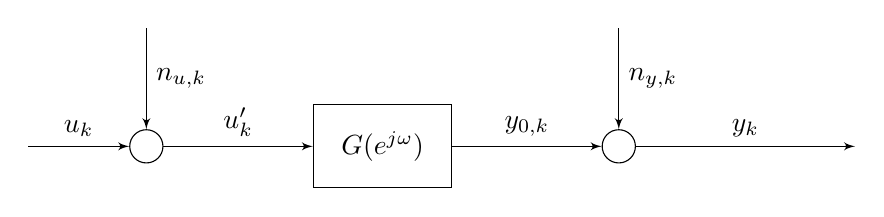
\begin{tikzpicture}[auto, node distance=3cm, >=latex']
    % 样式定义
    \tikzstyle{block} = [draw, rectangle, minimum height=3em, minimum width=5em, align=center]
    \tikzstyle{sum} = [draw, circle, node distance=1.5cm, minimum size=1.2em, inner sep=0pt]
    \tikzstyle{input} = [coordinate]
    \tikzstyle{output} = [coordinate]

    % 放置节点
    \node [input, name=input] {};
    \node [sum, right of=input] (sum1) {};
    \node [input,above of=sum1,node distance=1.5cm] (err_i) {};
    \node [block, right of=sum1] (G) {\(G(e^{j\omega})\)};
    \node [sum, right of=G,node distance=3cm] (sum2) {};
    \node [input,above of=sum2,node distance=1.5cm] (err_o) {};
    \node [output, right of=sum2] (output) {};

    \draw [->] (input) -- node {\(u_k\)} (sum1);
    \draw [->] (sum1) -- node {\(u'_k\)} (G);
    \draw [->] (G) -- node {\(y_{0,k}\)} (sum2);
    \draw [->] (sum2) -- node {\(y_k\)} (output);
    \draw [->] (err_i) -- node {\(n_{u,k}\)} (sum1);
    \draw [->] (err_o) -- node {\(n_{y,k}\)} (sum2);
\end{tikzpicture}
\end{center}

分析时域表达式为：
\begin{align*}
    y_k&=y_{0,k}+n_{y,k}\\
    &=g_k*u'_k+n_{y,k}\\
    &=g_k*[u_k+n_{u,k}]+n_{y,k}\\
    &=g_k*u_k+g_k*n_{u,k}+n_{y,k}
\end{align*}

等效的输出噪声为\(\omega_k = g_k*n_{u,k}+n_{y,k}\)。若输入侧噪声与输入信号本身不相关，那么输入信号就与输出噪声
不相关，所以依然可以得到无偏估计的脉冲响应序列。

但在实际工程中，输入侧噪声有时并不是完全的白噪声，而是和输入信号相关的噪声（如电阻压降对电压输入的敏感性）。极端情况下
输出侧测量噪声可能也是与输入信号相关。接下来对这种极端情况进行分析。

对时域表达式左右两边同时对\(u_k\)进行相关运算得到：
\begin{equation*}
    R_{uy}[k]=g_k*R_{uu}[k]+R_{u\omega}[k]
\end{equation*}

对\(R_{u\omega}[k]\)展开得到：
\begin{align*}
    R_{u\omega}[k] &= \text{E}[u_k\,\omega_{k+m}]\\
    &= \text{E}[u_k\times(g_k*n_{u,k+m}+n_{y,k+m})]\\
    &= \text{E}[u_k\times(g_k*n_{u,k+m})]+\text{E}[u_k\times n_{y,k+m}]\\
    &= (u_{-k}*g_k*n_{u,k})[k]+(u_{-k}*n_{y,k})[k]\\
    &= g_k*R_{un_u}[k]+R_{un_y}[k]
\end{align*}

上式中\(u_{-k}\)表示\(u_k\)的时序反转（与附录B中\(x_{-k}\)的约定一致），求取DTFT可得：
\begin{equation*}
    S_{u\omega}(e^{j\omega})=G(e^{j\omega})S_{un_u}(e^{j\omega})+S_{un_y}(e^{j\omega})
\end{equation*}

代入原式可得：
\begin{align*}
    S_{uy}(e^{j\omega})&=G(e^{j\omega})S_{uu}(e^{j\omega})+S_{u\omega}(e^{j\omega})\\
    &= G(e^{j\omega})S_{uu}(e^{j\omega})+G(e^{j\omega})S_{un_u}(e^{j\omega})+S_{un_y}(e^{j\omega})\\
    \hat{G}(e^{j\omega})=\cfrac{S_{yu}(e^{j\omega})}{S_{uu}(e^{j\omega})}&=G(e^{j\omega})+G(e^{j\omega})\cfrac{S_{un_u}(e^{j\omega})}{S_{uu}(e^{j\omega})}+\cfrac{S_{un_y}(e^{j\omega})}{S_{uu}(e^{j\omega})}
\end{align*}

整理可得：
\begin{equation}
    \hat{G}(e^{j\omega})=G(e^{j\omega})[1+\cfrac{S_{un_u}(e^{j\omega})}{S_{uu}(e^{j\omega})}]+\cfrac{S_{un_y}(e^{j\omega})}{S_{uu}(e^{j\omega})}
    \label{eq:开环带噪的有偏性公式}
\end{equation}

定义信噪比为\(\cfrac{S_{uu}(e^{j\omega})}{S_{un_u}(e^{j\omega})}\)和\(\cfrac{S_{uu}(e^{j\omega})}{S_{un_y}(e^{j\omega})}\)。根据\ref{eq:开环带噪的有偏性公式}可知，
信噪比越高，有偏估计的偏差越小，这也是工程上要求激励信号幅值较大的原因。

\setcounter{tocdepth}{3}
\addtocontents{toc}{\protect\setcounter{tocdepth}{3}}

\end{document}